%
% part1.tex
%
% (c) 2018 Prof Dr Andreas Müller, Hochschule Rapperswil
%
\begin{refsection}
%
% vorwort.tex -- Vorwort zum Buch zum Seminar
%
% (c) 2019 Prof Dr Andreas Mueller, Hochschule Rapperswil
%
\chapter*{Vorwort}
\lhead{Vorwort}
\rhead{}
Dieses Buch entstand im Rahmen des Mathematischen Seminars
im Frühjahrssemester 2023 an der Ostschweizer Fachhochschule in Rapperswil.
Die Teilnehmer, Studierende der Studiengänge für Elektrotechnik
und Bauingenieurwesen
der OST, erarbeiteten nach einer Einführung in das Themengebiet jeweils
einzelne Aspekte des Gebietes in Form einer Seminararbeit, über
deren Resultate sie auch in einem Vortrag informierten. 

Im Frühjahr 2023 war die harmonische Analysis das Thema des Seminars.
Ausgangspunkt war dabei die Idee, dass das Skalarprodukt von Funktionen
die ``Ähnlichkeit'' zweier Funktionen misst.
Damit lässt sich sowohl die klassische Fourier-Theorie ebenso motivieren
wie auch Verallgemeinerungen auf viele Situationen, in denen Funktionen
durch Approximation aus einer orthonormierten Funktionenfamilie gewonnen
werden.
Diese Vorgehensweise liegt einer grossen Zahl interessanter mathematischer
Methoden zu Grunde und führt auf eine breite Palette nützlicher
Konzepte.
Ausser den klassischen Integraltransformationen treten daher in diesem
Buch auch neuere Transformationen wie die Radon- oder M\'endez-Transformation
und ihre Anwendungen auf.

In einigen Arbeiten wurde auch Code zur Demonstration der 
besprochenen Methoden und Resultate geschrieben, soweit
möglich und sinnvoll wurde dieser Code im Github-Repository
\index{Github-Repository}%
dieses Kurses%
\footnote{\url{https://github.com/AndreasFMueller/SeminarHarmonischeAnalysis.git}}
\cite{buch:repo}
abgelegt.
Im genannten Repository findet sich auch der Source-Code dieses
Skriptes, es wird hier unter einer Creative Commons Lizenz
zur Verfügung gestellt.


\part{Grundlagen}
%
% chapter.tex -- Skalarprodukt
%
% (c) 2021 Prof Dr Andreas Müller, Hochschule Rapperswil
%
% !TeX spellcheck = de_CH
\chapter{Skalarprodukte
\label{buch:chapter:skalarprodukte}}
\kopflinks{Skalarprodukte}

%
% 1-definition.tex
%
% (c) 2023 Prof Dr Andreas Müller, OST Ostschweizer Fachhochschule
%
\section{Definition
\label{buch:opertoren:section:definition}}
\kopfrechts{Definition}


%
% 2-cauchyschwarz.tex
%
% (c) 2022 Prof Dr Andreas Müller, OST Ostschweizer Fachhochschule
%
\section{Ungleichungen
\label{buch:skalarprodukte:section:cauchyschwarz}}
\kopfrechts{Cauchy-Schwarz-Ungleichung}
In der Vektorgeometrie wird gelehrt, dass die Länge eines Vektors $u$
durch die Norm $\|u\|$ wiedergegeben wird und dass die geometrische
Intuition dazu passt.
Dazu gehört vor allem, dass die Dreiecksungleichung erfüllt ist,
dass also für drei Punkt $A$, $B$ und $C$
\begin{equation}
\overline{AB} \le \overline{AC} + \overline{BC}
\label{skalarprodukt:ungleichungen:eqn:dreieck}
\end{equation}
gilt.
In Vektorform bedeutet dies, dass
\[
\| b-a\|
\le
\| c-a\| + \|b-c\|.
\]
Schreibt man $u=c-a$ und $v=b-c$, dann ist $u+v=b-a$ und somit
\begin{equation}
\| u+v\| \le \|u\| + \|v\|.
\label{skalarprodukt:cauchyschwarz:eqn:dreieck0}
\end{equation}
Dies ist die Dreiecksungleichung in
Vektorform~\eqref{skalarprodukt:cauchyschwarz:eqn:dreieck0}.
Ziel dieses Abschnitts ist zu zeigen, dass jedes reelle oder
komplexe Skalarprodukt diese und weitere Eigenschaften automatisch
mitbringt.

%
% Cauchy-Schwarz-Ungleichung
%
\subsection{Cauchy-Schwarz-Ungleichung}
Sei also $\langle\;\,,\;\rangle$ ein reelles oder komplexes Skalarprodukt
auf dem Vektorraum $V$,
insbesondere ist $\langle v,v\rangle\ge 0$ für beliebige Vektoren $v\in V$.
Für zwei Vektoren $x,y\in V$ und $t\in \mathbb{R}$  gilt daher
\begin{align}
0
&\le
\| x+ty\|^2
=
\langle x+ty,x+ty\rangle
=
\langle x,x\rangle
+
t\langle x,y\rangle
+
t\langle y,x\rangle
+
t^2
\langle y,y\rangle.
\label{skalarprodukt:cauchyschwarz:eqn:quadrat}
\end{align}
Für ein reelles Skalarprodukt ist $\langle x,y\rangle=\langle y,x\rangle$
und damit
\begin{align}
0
&\le
\|x\|^2 + 2t\langle x,y\rangle + t^2 \|y\|^2.
\label{buch:skalarprodukt:cauchyschwarz:eqn:cspoly}
\end{align}
Dies ist ein quadratisches Polynom in der Variablen $t$, dessen Minimum
nicht negativ sein darf.

%
% Minimum eines quadratischen Polynoms
%
\subsubsection{Minimum eines quadratischen Polyoms}
Ein beliebiges quadratisches Polynom
\[
p(t)=at^2+bt+c
\]
kann durch
quadratisches Ergänzen in die Form
\[
p(t)
=
a\biggl(t+\frac{b}{2a}\biggr)^2 -\frac{b^2}{4a}+c
\]
gebracht werden.
Daraus kann man ablesen, dass das Minimum an der Stelle
\[
t_0
=
-\frac{b}{2a}
\]
angenommen wird und den Wert 
\begin{equation}
p(t_0)
=
c-\frac{b^2}{4a}
\end{equation}
hat.
Die gleiche Lösung kann natürlich auch durch Bestimmung des Minimums
von $p(t)$ mit Hilfe der Bedingung $p'(t_0)=0$ gefunden werden.

%
% Cauchy-Schwarz-Ungleichung für einen reellen Vektorraum
%
\subsubsection{Cauchy-Schwarz-Ungleichung für einen reellen Vektorraum}
Für~\eqref{buch:skalarprodukt:cauchyschwarz:eqn:cspoly}
ist
\[
a=\|y\|^2,\quad
b=2\langle x,y\rangle
\quad\text{und}\quad
c=\|x\|^2.
\]
Daher folgt aus~\eqref{buch:skalarprodukt:cauchyschwarz:eqn:cspoly}
\[
0
\le
\|x\|^2 - \frac{\langle x,y\rangle^2}{\|y\|^2}
\qquad\Rightarrow\qquad
\langle x,y\rangle^2 \le \|x\|^2\, \|y\|^2
\qquad\Rightarrow\qquad
|\langle x,y\rangle| \le \|x\|\, \|y\|.
\]
Dies ist die Cauchy-Schwarz-Ungleichung für das Skalarprodukt
$\langle \;\,,\;\rangle$.

\begin{satz}[Cauchy-Schwarz]
\label{buch:skalarprodukt:cauchy-schwarz:satz:reell}
Ein reelles Skalarprodukt $\langle\;\,,\;\rangle$ auf dem reellen Vektorraum
$V$ erfüllt die Cauchy-Schwarz-Ungleichung
\[
|\langle x, y\rangle| \le \|x\|\,\|y\|
\]
für $x,y\in V$.
\end{satz}

%
% Cauchy-Schwarz-Ungleichung für einen komplexen Vektorraum
%
\subsubsection{Cauchy-Schwarz-Ungleichung für einen komplexen Vektorraum}
Für ein komplexes Skalarprodukt ist das Produkt $\langle x,y\rangle$
nicht mehr unbedingt reell und kann damit nicht mehr direkt mit den
Normen $\|x\|^2u$ und $\|y\|^2$ vergleichen.
Wir ersetzen daher $t$ durch
$t\langle y,x\rangle=t\overline{\langle x,y\rangle}$
und erhalten 
\begin{align*}
0
\le
\|x+t\langle y,x\rangle y\|^2
&=
\langle x,x\rangle
+t\langle y,x\rangle \langle x,y\rangle
+t\overline{\langle y,x\rangle}\langle y,x\rangle
+t^2\langle y,y\rangle
\\
&=
\|x\|^2
+
t
2|\langle x,y\rangle|^2
+
t^2 |\langle x,y\rangle|^2
\|y\|^2.
\end{align*}
Dies ist wieder ein quadratisches Polynom, diesmal mit den Koeffizienten
\[
a= |\langle x,y\rangle|^2 \|y\|^2,
\quad
b= 2|\langle x,y\rangle|^2
\quad\text{und}\quad
c= \|x\|^2.
\]
Das Minimum dieses Polynoms ist nach
\[
0
\le
c-\frac{b^2}{4a}
=
\|x\|^2 - \frac{|\langle x,y\rangle|^4}{|\langle x,y\rangle|^2\,\|y\|^2}
=
\|x\|^2 - \frac{|\langle x,y\rangle|^2}{\|y\|^2}
\quad\Rightarrow\quad
|\langle x,y\rangle|^2 \le \|x\|^2\,\|y\|^2
\quad\Rightarrow\quad
|\langle x,y\rangle \le \|x\|\,\|y\|.
\]
Dies ist die Cauchy-Schwarz-Ungleichung für einen komplexen Vektorraum.

\begin{satz}[Cauchy-Satz]
\label{buch:skalarprodukt:cauchy-schwarz:satz:komplex}
Ein komplexes Skalarprodukt $\langle\;\,,\;\rangle$ auf dem komplexen Vektorraum
$V$ erfüllt die Cauchy-Schwarz-Ungleichung
\[
|\langle x, y\rangle| \le \|x\|\,\|y\|
\]
für $x,y\in V$.
\end{satz}

Man beachte, dass die
Sätze~\ref{buch:skalarprodukt:cauchy-schwarz:satz:reell}
und
\ref{buch:skalarprodukt:cauchy-schwarz:satz:komplex}
nur die Axiome eines Skalarproduktes verwenden.
Sie gelten also
ganz unabhängig von der konkreten Definition des Skalarproduktes,
solange die Eigenschaften eines Skalarproduktes gegeben sind.

\begin{beispiel}
Die sesquilineare Funktion
\[
\langle x,y\rangle
=
\sum_{i=1}^n\overline{x}_i y_i
\]
für Vektoren $x,y\in\mathbb{C}^n$ ist positiv definit, denn
\[
\langle x,x\rangle
=
\sum_{i=1}^n \overline{x}_i x_i = \sum_{i=1}^n |x_i|^2 > 0
\]
für $x\ne 0$.
Nach Satz~\ref{buch:skalarprodukt:cauchy-schwarz:satz:komplex}
gilt daher
\[
\biggl|
\sum_{i=1}^n \overline{x}_i y_i
\biggr|
\le
\sqrt{\sum_{i=1}^n |x_i|^2} \sqrt{\sum_{i=1}^n |y_i|^2}
\quad\text{oder auch}\quad
\biggl|
\sum_{i=1}^n x_i y_i
\biggr|
\le
\sqrt{\sum_{i=1}^n |x_i|^2} \sqrt{\sum_{i=1}^n |y_i|^2}
\]
für beliebige Vektoren $x,y\in\mathbb{C}^n$.
\end{beispiel}

\begin{beispiel}
Die sesquilineare Funktion
\[
\langle f,g\rangle
=
\int_a^b \overline{f(x)} g(x)\,dx
\]
für komplexwertige, stetige Funktion auf dem Intervall $[a,b]$
ist positiv definit, denn
\[
\langle f,f\rangle
=
\int_a^b \overline{f(x)} f(x)\,dx
=
\int_a^b |f(x)|^2\,dx
\ge 0
\]
für $f\ne 0$.
Nach Satz~\ref{buch:skalarprodukt:cauchy-schwarz:satz:komplex}
gilt daher
\begin{align*}
\biggl|\int_a^b \overline{f(x)}g(x)\,dx\biggr|
&\le
\sqrt{\int_a^b |f(x)|^2\,dx}
\sqrt{\int_a^b |g(x)|^2\,dx}
\intertext{oder auch}
\biggl|\int_a^b f(x) g(x)\,dx\biggr|
&\le
\sqrt{\int_a^b |f(x)|^2\,dx}
\sqrt{\int_a^b |g(x)|^2\,dx}
\end{align*}
für beliebige komplexwertige stetige Funktionen $f,g$ auf dem
Intervall $[a,b]$.
\end{beispiel}

%
% Dreiecksungleichung
%
\subsection{Dreiecksungleichung}
Die Intuition einer Längenmessung basiert auf der
Dreiecksungleichung~\eqref{skalarprodukt:ungleichungen:eqn:dreieck}.
Sie ist gleichbedeutend mit der
Vektorform~\eqref{skalarprodukt:cauchyschwarz:eqn:dreieck0}
der Ungleichung.

Die Cauchy-Schwarz-Ungleichung ermöglicht nun, diese Ungleichung
nachzurechnen.
Die Norm von $\|x+y\|^2$ ist
\[
\|x+y\|^2
=
\langle x+y,x+y\rangle
=
\langle x,x\rangle
+
\langle x,y\rangle
+
\langle y,x\rangle
+
\langle y,y\rangle
=
\|x\|^2 + 2\operatorname{Re}\langle x,y\rangle + \|y\|^2.
\]
Den mittleren Term kann man mit der Cauchy-Schwarz-Ungleichung
umformen:
\begin{align*}
\|x\|^2 + 2\operatorname{Re}\langle x,y\rangle + \|y\|^2.
&\le
\|x\|^2 + 2|\operatorname{Re}\langle x,y\rangle| + \|y\|^2.
\\
&\le
\|x\|^2 + 2|\langle x,y\rangle| + \|y\|^2.
\\
&\le
\|x\|^2 + 2\|x\|\,\|y\| + \|y\|^2
=
(\|x\| + \|y\|)^2.
\end{align*}
Durch Ziehen der Wurzel folgt
\[
\|x+y\| \le \|x\| + \|y\|.
\]
Damit ist der folgende Satz bewiesen.

\begin{satz}[Dreiecksungleichung]
Für die Norm zu einem beliebigen Skalarprodukt auf dem reellen
oder komplexen Vektorraum $V$ gilt die Dreiecksungleichung
\[
\|x+y\| \le \|x\| + \|y\|
\]
für $x,y\in V$.
\end{satz}

%
% Normen
%
\subsection{Normen
\label{skalarprodukt:cauchyschwarz:subsection:norm}}
Das Skalarprodukt ist nicht die einzige Möglichkeit, eine Norm auf
einem Vektorraum zu definieren.
Zum Beispiel kann man auf $\mathbb{C}^n$ die sogenannte $l^1$-Norm
definieren.

\begin{definition}
Die Funktion
\[
\|x\|_1
=
\sum_{i=1}^n |x_i|
\]
für $x\in\mathbb{C}^n$ heisst die {\em $l^1$-Norm} auf $\mathbb{C}^n$.
\end{definition}

Die Funktion $\|\cdot\|_1$ ist eine Norm im Sinne der folgenden Definition.

\begin{definition}
Eine Funktion $\|\cdot\| \colon V\to\mathbb{R}$ auf einem reellen
oder komplexen Vektorraum $V$ heisst eine {\em Norm}, wenn Sie die
folgenden Bedingungen erfüllt
\begin{enumerate}
\item
$\|\lambda x\| = |\lambda|\, \|x\|$ für $x\in V$ und $\lambda\in \Bbbk$
\item
Für alle Vektoren $x\in V$ mit $x\ne 0$ gilt $\|x\|>0$.
\item
Dreiecksungleichung: $\|x+y\| \le \|x\| + \|y\|$ für alle $x,y\in V$
\end{enumerate}
\end{definition}

Es ist klar, dass die $l^1$-Norm die Bedingungen~1 und 2 erfüllt.
Aber auch die Bedingung~3 kann man leicht  nachprüfen:
\[
\|x+y\|_1
=
\sum_{i=1}^n |(x+y)_i|
=
\sum_{i=1}^n |x_i+y_i|
\le
\sum_{i=1}^n(|x_i|+|y_i|)
=
\sum_{i=1}^n|x_i|
+
\sum_{i=1}^n|y_i|
=
\|x\|_1 + \|y\|_1,
\]
wozu wir nur die Dreiecksungleichung $|a+b|\le |a| + |b|$ für reelle 
oder komplexe Zahlen $a,b$ benötigen.

\begin{beispiel}
Die Funktion
\[
\|x\|_\infty = \sup_{1\le i\le n} |x_i|
\]
ist eine Norm auf $\mathbb{C}^n$.
\end{beispiel}

Auch in diesem Fall sind die Bedingungen~1 und 2 ganz offensichtlich erfüllt.
Für die Dreiecksungleichung rechnen
\begin{align*}
\|x+y\|_\infty
&=
\sup_{1\le i\le n} |x_i+y_i|
\le
\sup_{1\le i\le n} (|x_i|+|y_i|)
\le
\sup_{1\le i\le n} |x_i|+\sup_{1\le i\le n}|y_i|
=
\|x\|_\infty + \|y\|_\infty.
\end{align*}
Somit ist $\|\cdot\|_\infty$ eine Norm auf $\mathbb{C}^n$.

%
% Polaridentität
%
\subsection{Polaridentität}
Die durch das Skalarprodukt definierte Norm
\( \|x\|^2=\langle x,x\rangle \)
ist nach Abschnitt~\ref{skalarprodukt:cauchyschwarz:subsection:norm}
ein Spezialfall einer Norm.
Ist es möglich, für eine Norm, die von einem Skalarprodukt herkommt,
das Skalarprodukt wieder zu rekonstruieren?

%
% Reelles Skalarprodukt aus der Norm
%
\subsubsection{Reelles Skalarprodukt aus der Norm}
Die Antwort gibt der folgende Satz.

\begin{satz}[Polaridentität]
\label{skalarprodukt:cauchyschwarz:satz:polarformel}
Ist $\|\cdot\|$ die Norm zu einem Skalarprodukt auf dem reellen Vektorraum
$V$, dann kann das Skalarprodukt zweier Vektoren $x,y\in V$ mittels
der sogenannten {\em Polaridentität}
\index{Polaridentität}%
\begin{equation}
\langle x, y\rangle
=
\frac12\bigl(
\|x+y\|^2 - \|x\|^2 - \|y\|^2 
\bigr)
\label{skalarprodukt:cauchyschwarz:eqn:polar}
\end{equation}
berechnet werden.
\end{satz}

\begin{proof}[Beweis]
Die Gleichung
\begin{align*}
\|x+y\|^2
&=
\langle x+y,x+y\rangle
=
\|x\|^2 + 2\langle x,y\rangle + \|y\|^2 
\end{align*}
kann nach $\langle x,y\rangle$ aufgelöst werden und ergibt
die behauptete Formel~\eqref{skalarprodukt:cauchyschwarz:eqn:polar}.
\end{proof}

% 
% Parallelogrammgleichung
%
\subsubsection{Parallelogrammgleichung}
\begin{figure}
\centering
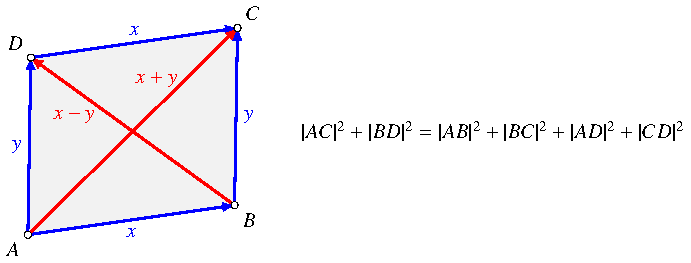
\includegraphics{chapters/010-skalarprodukt/images/parallelogramm.pdf}
\caption{Parallelogrammregel für eine Norm, die aus einem Skalarprodukt
entsteht.
\label{skalarprodukt:cauchyschwarz:fig:parallelogramm}}
\end{figure}
Die Polaridentitäten können auch noch in einer anderen Form geschrieben
werden.
Dazu berechnet man zusätzlich die Norm von $x-y$:
\begin{align*}
\|x+y\|^2
&=
\|x\|^2 + \|y\|^2 + 2\langle x, y\rangle
\\
\|x-y\|^2
&=
\|x\|^2 + \|y\|^2 - 2\langle x, y\rangle
\\
\|x+y\|^2 +\|x-y\|^2
&=
2\|x\|^2 + 2\|y\|^2
\end{align*}

\begin{satz}
\label{skalarprodukt:cauchyschwarz:satz:parallelgramm}
Für eine Norm, die von einem reellen Skalarprodukt herkommt, gilt die
Parallelogrammformel
\begin{equation}
\|x+y\|^2 +\|x-y\|^2
=
2\|x\|^2 + 2\|y\|^2.
\label{skalarprodukt:cauchyschwarz:eqn:parallelgramm}
\end{equation}
(Abbildung~\ref{skalarprodukt:cauchyschwarz:fig:parallelogramm})
\end{satz}

Das Skalarprodukt kann man damit auf verschiedene Weise aus der
Norm gewinnen:
\begin{equation}
\begin{aligned}
\langle x, y\rangle
&=
{\textstyle\frac12}\bigl( \|x\|^2 + \|y\|^2 - \|x+y\|^2 \bigr)
\\
&=
{\textstyle\frac12}\bigl(
\|x+y\|^2
-
\|x\|^2 
-
\|y\|^2
\bigr)
\\
&=
{\textstyle\frac14}\bigl(
\|x+y\|^2 - \|x-y\|^2
\bigr).
\end{aligned}
\label{skalarprodukt:cauchyschwarz:eqn:realteil}
\end{equation}
Nur die letzte Formel ist noch nicht gut begründet.
Man kann aber sofort nachrechnen, dass 
\begin{align*}
\|x+y\|^2&=\|x\|^2+2\langle x,y\rangle+\|y\|^2\\
\|x-y\|^2&=\|x\|^2-2\langle x,y\rangle+\|y\|^2
\intertext{die Differenz}
\|x+y\|^2 - \|x-y\|^2 &= 4\langle x,y\rangle
\qquad
\Rightarrow
\qquad
\langle x,y\rangle
=
\frac14\bigl(\|x+y\|^2 - \|x-y\|^2\bigr)
\end{align*}
haben.

%
% Komplexes Parallelogramm aus der Norm
%
\subsubsection{Komplexe Skalarprodukt}
Das Resultat von Satz~\ref{skalarprodukt:cauchyschwarz:satz:polarformel}
gilt in abgeänderter Form auch für komplexe Skalarprodukte.
Da das Skalarprodukt auch einen nichtverschwindenen Imaginärteil haben
kann, wird eine zusätzliche Gleichung zur Berechnung des Imaginärteils
nötig.
Eine solche kann gewonnen werden, indem zusätzlich die Normen
$\|x+iy\|^2$ und $\|x-iy\|^2$ berechnet werden.
Dazu ist zu beachten, dass
\[
\langle x,y\rangle
-
\langle y,x\rangle
=
\langle x,y\rangle
-
\overline{
\langle x,y\rangle
}
=
2i\operatorname{Im}\langle x,y\rangle
\]
Damit erhält man
\begin{align*}
\|x+iy\|^2 &= \|x\|^2 + i\langle x,y\rangle - i\langle y,x\rangle + \|y\|^2 
           = \|x\|^2 + 2\operatorname{Im}\langle x,y\rangle + \|y\|^2 \\
\|x-iy\|^2 &= \|x\|^2 - i\langle x,y\rangle + i\langle y,x\rangle + \|y\|^2 
           = \|x\|^2 - 2\operatorname{Im}\langle x,y\rangle + \|y\|^2.
\end{align*}
Damit kann man nach dem Imaginärteil des Skalarproduktes auflösen und
die Formeln
finden, die den Formeln
\eqref{skalarprodukt:cauchyschwarz:eqn:realteil}
für das reelle Skalarprodukt entsprechen.
\eqref{skalarprodukt:cauchyschwarz:eqn:realteil}
Formeln bleiben gültig als Formeln für den Realteil des Skalarproduktes.
Damit haben wir den folgenden Satz gefunden.

\begin{satz}[Polaridentitäten für ein komplexes Skalarprodukt]
Ist $\|\cdot\|$ die Norm, die aus dem komplexen Skalarprodukt
$\langle\;\,,\;\rangle$ auf einem Vektorraum $V$ gewonnen wurde,
dann können Real- und Imaginärteil mit den Formeln
\begin{align*}
\operatorname{Re}\langle x,y\rangle
&=
{\textstyle\frac12}\bigl(
\|x+y\|^2 - \|x\|^2 -\|y\|^2
\bigr)
\\
&=
{\textstyle\frac12}\bigl(
\|x\|^2 +\|y\|^2 - \|x+y\|^2
\bigr)
\\
&=
{\textstyle\frac14}\bigl(
\|x+y\|^2 - \|x-y\|^2
\bigr),
\\
\operatorname{Im}\langle x,y\rangle
&=
{\textstyle\frac12}\bigl(
\|x+iy\|^2-\|x\|^2-\|y\|^2
\bigr)
\\
&=
{\textstyle\frac12}\bigl(
\|x\|^2+\|y\|^2-\|x-iy\|^2
\bigr)
\\
&=
{\textstyle\frac14}\bigl(
\|x+iy\|^2
-
\|x-iy\|^2
\bigr)
\end{align*}
für beliebige Vektoren $x,y\in V$
allein aus Werten der Norm berechnet werden.
\end{satz}


%
% 3-funktionenraeume.tex
%
% (c) 2022 Prof Dr Andreas Müller, OST Ostschweizer Fachhochschule
%
\section{Funktionenräume
\label{buch:skalarprodukt:section:funktionenraeume}}
\kopfrechts{Funktionenräume}
Ziel der harmonischen Analysis ist die effiziente Approximation einer
grossen Klasse von Funktionen.
Als approximierende Funktionen kommen stetige Funktionen, Polynome,
trigonometrische Polynome oder eine ähnlich, einfach konstruierbare
Funktionenfamilie in Frage.
Es gilt zunächst herauszufinden, was ``Approximation'' genau heissen
soll und von welchen Funktionen man überhaupt erwarten kann, dass sie
approximiert werden können.

%
% Stetige Funktionen
%
\subsection{Stetige Funktionen
\label{buch:skalarprodukt:subsection:stetige-funktionen}}
Der frühe intuitive Funktionsbegriff ging oft von der Vorstellung einer
in einem Strich gezeichneten Kurve aus, wie man sie von den Graphen
der Polynome oder der trigonometrischen Funktionen her kennt.
In moderner Sprechweise sind dies die stetigen Funktionen.

\begin{definition}
Eine Funktion $f\colon I\to\mathbb{R}$ mit $I\subset \mathbb{R}$
heisst stetig in einem Punkt $x_0\in I$, wenn für jedes $\varepsilon>0$
ein $\delta>0$ existiert derart, dass $f(x)-f(x_0)|<\delta$ sobald
$|x-x_0|<\varepsilon$.
\end{definition}

Nur die Eigenschaft, eine Abstandsmessung zu besitzen, wird vom
Definitionsbereich $I\subset \mathbb{R}$ verlangt.
Der Stetigkeitsbegriff kann daher verallgemeinert werden auf den
Begriff des metrischen Raumes.

\begin{definition}
Eine {\em Metrik} auf einer Menge $X$ ist eine Funktion
\index{Metrik}%
$d\colon X\times X\to \mathbb{R}$
mit den folgenden Eigenschaften
\begin{enumerate}
\item
Positiv definit: $d(x,y)\ge 0$ und $d(x,y)$ genau dann, wenn $x=y$.
\item
Symmetrie: \(d(x,y)=d(y,x)\)
\item
Dreiecksungleichung: \( d(x,y) \le d(x,z) + d(z,y) \).
\end{enumerate}
Ein {\em metrischer Raum} ist ein Menge $X$ mit einer Metrik.
\index{matrischer Raum}%
\end{definition}

In einem metrischen Raum ist der Begriff des Grenzwertes übertragbar.
Mit dem Begriff des Grenzwertes lässt sich auch der Begriff der
Stetigkeit verallgemeinern.

\begin{definition}
Ist $x_n\in X$ eine Folge von Punkten in einem metrischen Raum $X$,
dann heisst $x$ der Grenzwert der Folge $x_n$, wenn es für jedes
$\varepsilon>0$ ein $N>0$ gibt derhart, dass
$d(x_n,x)\le \varepsilon$ für alle $n>N$.
Eine Funktion $f\colon X\to Y$ zwischen metrischen Räumen heisst
stetig im Punkt $x\in X$, wenn für jede Folge $x_n\in X$ mit
Grenzwert $x$ auch die Folge $y_n=f(x_n)\in Y$ konvergiert und
den Grenzwert $y=f(x)$ hat.
\end{definition}

Teilmengen von $\mathbb{R}$ oder $\mathbb{R}^n$ tragen natürlich
die Struktur eines metrischen Raumes mit der Abstandsmessung in 
$\mathbb{R}^n$ als Metrik
\[
d(x,y) = \sqrt{(x_1-y_1)^2 + \ldots + (x_n-y_n)^2} = \|x-y\|.
\]
Die Eigenschaften einer Metrik wurden bereits in Abschnitt
\ref{buch:skalarprodukte:section:cauchyschwarz} nachgewiesen.

Der Begriff des Grenzwertes klärt, was mit der Approximation von $x$
durch eine Folge $x_n$ gemeint ist.
Wenn man darauf aufbauend die Konvergenz einer Folge von Funktionen
gegen eine Grenzfunktion definieren will, braucht man einen Abstansbegriff
zwischen Funktionen.
Ein erster Versuch könnte sein, als Abstand zwischen zwei Funktionen
$f$ und $g$ die Funktion
\[
d(f,g) = |f(x_0) - g(x_0)|.
\]
Die Menge der Funktionen wird dadurch jedoch nicht zu einem metrischen
Raum.
Zwar gilt sicher die Symmetrie und Dreiecksungleichung, und auch 
$d(f,g)\ge 0$ für beliebige Funktionen.
Aber wenn $d(f,g)=0$ ist, heisst das nur, dass $f$ und $g$ im Punkt
$x_0$ den gleichen Wert haben.
Ausser in trivialen Fällen wird es Funktionen geben, die zwar im Punkt
$x_0$ übereinstimmen, sich aber in mindestens einem anderen Punkt
unterscheiden.

%
% Normierte Räume
%
\subsubsection{Normierte Räume}
Die stetigen Funktionen bilden aber keine strukturlose Menge, sie
bilden einen Vektorraum: die Summe von stetigen Funktionen ist ebenfalls
stetig, multiplizieren einer stetigen Funktion mit einem Skalar führt
nicht aus der Menge der stetigen Funktionen heraus.
Die für den Grenzwertbegriff von Funktionen verwendete Abstandsmessung 
sollte der Vektorraumstruktur ebenfalls Rechnung tragen.

\begin{definition}
\label{buch:skalaprodukt:funktionenraume:def:norm}
Sei $V$ ein Vektorraum über $\mathbb{R}$, dann heisst eine Funktion
\( \|\;\cdot\;\| \colon V \to \mathbb{R}\) eine {\em Norm}, wenn gilt
\index{Norm}
\begin{enumerate}
\item
Definit: $ \|x\| = 0 \Rightarrow x=0$
\item
Homogeneität: $ \| \lambda x \| = |\lambda| \cdot \|x\|$
\item
Dreiecksungleichung: $\|x+y\| \le \|x\| + \|y\|$
\end{enumerate}
Ein {\em normierter Raum} ist ein Vektorraum $V$ mit einer Norm.
\end{definition}

%
% Vollständigkeit
%
\subsubsection{Vollständigkeit}
In den rationalen Zahlen hat nicht jede Folge einen Grenzwert.
Die Zahl $\sqrt{2}$ lässt sich beliebig genau durch rationale Zahlen
approximieren, sie ist aber nicht in $\mathbb{Q}$.
Ähnlich lässt sich die Funktion $x\mapsto \sqrt{x}$ beliebig genau 
durch Polyome approximieren, sie ist aber selbst kein Poylnome

\begin{definition}
Ein Folge $x_n\in X$ in einem metrischen Raum heisst {\em Cauchy-Folge},
wenn es für jedes $\varepsilon>0$ ein $N>0$ gibt derart, dass 
$|x_n-x_m|<\varepsilon$ wenn $n,m>N$ ist.
\end{definition}

Cauchy-Folgen sind also Folgen, die sich für genügend grossen Index
kaum mehr ändern und für die man daher Konvergenz erwarten würde.

\begin{definition}
Ein normierter Raum heisst {\em vollständig} oder ein Banach-Raum,
wenn jede Cauchy-Folge einen Grenzwert hat.
\end{definition}

Die rationalen Zahlen $\mathbb{Q}$ bilden keinen vollständigen
metrischen Raum, aber die reellen Zahlen $\mathbb{R}$ enthalten
alle Grenzwerte von Cauchy-Folgen, $\mathbb{R}$ ist eine vollständiger
metrischer Raum.
Die Menge der Polynome, betrachtet als Teilmenge der Menge der
stetigen Funktionen $[0,1]\to\mathbb{R}$ ist nicht vollständig,
da es eine Folge $f_n(x)$ von Approximationsfunktionen der Funktion
$x\mapsto \sqrt{x}$ gibt.
Als Cauchy-Folge konvergiert sie zwar gegen eine stetige Funktion,
aber die Grenzfunktion ist nicht mehr im Raum der Polynome.

Das Ziel der folgenden Kapitel ist also, zu geeignet interessanten
Funktionenfamilien ``gute'' Normen zu finden derart, dass Cauchy-Folgen
konvergieren gegen Funktionen, die immer noch ausreichend viele
nützliche Eigenschaften haben.
Im besten Fall konvergieren stetige Funktionen gegen stetige Funktionen,
es wird sich aber zeigen, dass diese Anforderung zu streng ist.

%
% Norm fpr stetige Funktionen
%
\subsection{Norm für stetige Funktionen
\label{buch:skalarprodukt:subsection:normfuerstetigefunktionen}}
Damit man von Konvergenz von Folgen stetiger Funktionen sprechen kann,
brauchen wir jetzt also eine Norm für stetige Funktionen.

\begin{definition}
Sei $X$ ein metrischer Raum und
\[
C(X)
=
C_{\mathbb{R}}(X)
=
\{
f\colon X \to\mathbb{R}\mid
\text{$f$ ist stetig}
\}
\]
der Vektorraum der stetigen Funktion auf $X$.
Die Norm von $C(X)$ ist definiert als
\[
\|f\| = \sup_{x\in X} |f(x)|.
\]
Sie heisst die {\em Supremum-Norm}.
\end{definition}

Wir prüfen nach, dass die Supremum-Norm tatsächlich eine Norm ist.
Dazu sind die definierenden Eigenschaften nachzurechnen:
\begin{enumerate}
\item Definit: 
\[
0
=
\|f\|
=
\sup_{x\in X} |f(x)|
\quad\Rightarrow\quad
f(x)=0 \;\forall x\in X
\quad\Rightarrow\quad
f\in C(X).
\]
\item Homogeneität:
\[
\|\lambda f\|
=
\sup_{x\in X} |\lambda f(x)|
=
|\lambda| \sup_{x\in X} |f(x)|
=
|\lambda| \cdot \|f\|.
\]
\item
Dreiecksungleichung:
\[
\|f+g\|
=
\sup_{x\in X}|f(x)+g(x)|
\le
\sup_{x\in X}(|f(x)|+|g(x)|)
\le
\sup_{x\in X}|f(x)|+\sup_{x\in X}|g(x)|
=
\|f\| + \|g\|.
\]
\end{enumerate}

Eine Cauchy-Folge $f_n$ von Funktionen $X\to \mathbb{R}$ hat die
Eigenschaft, dass für jedes $\varepsilon >0$ ein $N>0$ existiert,
derart dass $\|f_n-f_m\|<\varepsilon$ ist.
Da die Norm der maximale Unterschied von Funktionswerten ist,
folgt dass für eine Cauchy-Folge in $C(X)$ die Folge $f_n(x)$ eine
Cauchy-Folge in $\mathbb{R}$ ist und damit einen Grenzwert in $\mathbb{R}$
hat.
Die Funktion $f(x) = \lim_{n\to\infty}f_n(x)$ ist die Grenzfunktion.
Die Konvergenz bezüglich der Norm besagt, dass für jedes $\varepsilon>0$
es ein $N>0$ gibt derart, dass
\[
\varepsilon 
>
\|f_n-f\|
\ge 
|f_n(x)-f(x)|
\]
ist für alle $n>N$ und unabhängig von $x\in X$.
Die Konvergenz bezüglich der $\|\;\cdot\;\|$-Norm ist also die wohlbekannte
gleichmässige Konvergenz.
Es kann gezeigt werden, dass die Grenzfunktion wieder stetig ist.

\begin{satz}
Der Raum der stetigen Funktion $C(X)$ mit der Supremumg-Norm ist
ein Banach-Raum.
\end{satz}

%
% Skalarprodukt
%
\subsection{Skalarprodukt
\label{buch:skalarprodukt:subsection:skalarprodukt}}
\begin{figure}
\centering
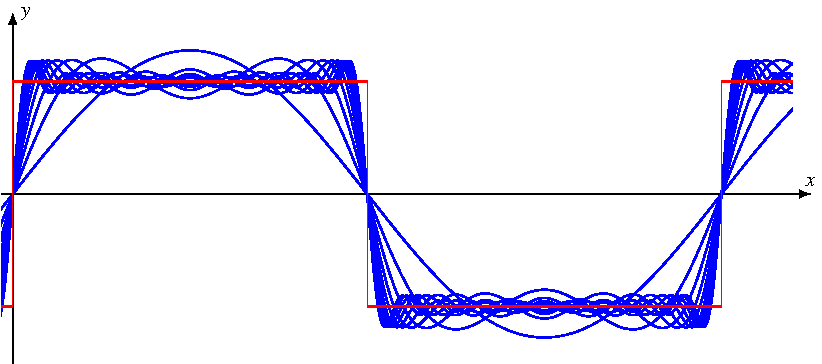
\includegraphics{chapters/010-skalarprodukt/images/fourierrechteck.pdf}
\caption{Approximation der Rechteckfunktion (rot) durch eine Folge
von Partialsummen der Fourier-Reihe.
\label{buch:skalarprodukt:fig:fourierrechteck}}
\end{figure}%
Die Supremum-Norm auf dem Raum der stetigen Funktionen hat den
Begriff der gleichmässig konvergenten Funktionenfolgen ergeben.
Cauchy-Folgen von stetigen Funktionen in der Supremum-Norm konvergieren
wieder gegen eine stetige Funktione.
Ist eine Funktion nicht stetig, lässt Sie sich im Sinne der Supremum-Norm
nicht durch stetige Funktionen approximieren.
Andererseits hat Fourier gezeigt, wie man technische wichtige Funktionen
wie die Rechteckfunktion durch trigonometrische Polynome
\begin{equation}
f_n(x)
=
\frac{4}{\pi} \sum_{k=0}^n \frac{\sin kx}{k}
=
\frac{4}{\pi} \biggl(
\sin x
+
\frac{\sin 3x}{3}
+
\frac{\sin 5x}{5}
+
\frac{\sin 7x}{7}
+
\ldots
\biggr)
\label{buch:skalarprodukt:eqn:rechteckreihe}
\end{equation}
approximieren kann.
Diese sind alle stetig und kommen der Rechteckfunktion in jedem Punkt,
in dem die Funktion stetig ist, beliebig nahe.
An den Stellen $x = n\pi$ hat die Grenzfunktion eine Sprungstelle,
die approximierenden Funktionen haben dort immer Abstand $1$
(siehe Abbildung~\ref{buch:skalarprodukt:fig:fourierrechteck}).
Die Folge ist also keine Cauchy-Folge und sie konvergiert nicht im
Sinne der Supremum-Norm.
Für solche Anwendungen muss eine besser geeignete Norm gefunden werden,
in der die Folge konvergiert.

%
% Skalarprodukt von Funktion
%
\subsubsection{Die $L^1$-Norm einer Funktion}
Die Supremum-Norm sieht nur den grössten Wert, die Konvergenz der Folge
\eqref{buch:skalarprodukt:eqn:rechteckreihe} ist aber nicht gleichmässig,
die maximale Abweichung ist immer $1$.
Gesucht ist eine Norm, die für die Folge
\eqref{buch:skalarprodukt:eqn:rechteckreihe} 
nur im Mittel eine Abweichung feststellt.
Für die Berechnung des Mittelwerts kann das Integral verwendet werden:

\begin{definition}
\label{buch:skalaprodukt:definition:l1norm}
Für eine stetige Funktion $X\to\mathbb{R}$, für die $x\mapsto |f(x)|$
integrierbar ist, heisst
\begin{equation}
\|f\|_1 = \int_X |f(x)|\,dx
\label{buch:skalarprodukt:eqn:l1norm}
\end{equation}
die {\em $L^1$-Norm} der Funktion $f$.
\end{definition}

Die $L^1$-Norm ist tatsächlich eine Norm, wir verifizieren die
definierenden Eigenschaften einer Norm.
\begin{enumerate}
\item
Definit: Sei $f$ eine stetige Funktion mit $\|f\|_1=0$
Wäre $f\ne 0$, dann gäbe es einen Punkt $x_0\in X$ mit $f(x_0) \ne 0$.
Da $f$ stetig ist, ist $f|(x)| > \frac12|f(x_0)|$ für $x$ in einer
$\delta$-Umgebung von $x_0$.
Dann folgt für die $L^1$-Norm
\begin{align*}
\|f\|_1
=
\int_X |f(x)|\,dx
\ge
\frac12 |f(x_0)| \cdot \delta 
> 0.
\end{align*}
Dies widerspricht der Annahme, dass $\|f\|_1=0$ ist, also muss $f=0$ sein.
\item
Homogeneität folgt durch direkte Rechnung
\[
\|\lambda f\|_1
=
\int_X |\lambda f(x)|\,dx
=
|\lambda|
\int_X |f(x)|\,dx
=
|\lambda| \cdot \|f\|.
\]
\item
Die Dreiecksungleichung folgt aus
\[
\|f+g\|_1
=
\int_X |f(x) + g(x)|\,dx
\le
\int_X |f(x)| + |g(x)|\,dx
=
\int_X |f(x)| + \int_X |g(x)|\,dx
=
\|f\|_1 + \|g\|_1.
\]
\end{enumerate}

Die $L^1$-Norm ist etwas ``schwächer'' als die Supremum-Norm im
folgenden Sinne.
Eine in der Supremum-Norm konvergente Funktionenfolge auf einem
kompakten Definitionsbereich $X$ ist auch in der $L^1$-Norm konvergent.
Zur Unterscheidung der verschiedenen Normen werden wir in Zukunft die
Supremum-Norm manchmal auch als $\|f\|_{\infty} = \|f\|$ schreiben.

\begin{satz}
Ist $X$ eine kompakte Teilmenge von $\mathbb{R}$ und $f_n$ eine
in der Supremum-Norm konvergente Folge stetiger Funktionen $f_n$,
dann ist $f_n$ auch in der $L^1$-Norm konvergent.
\end{satz}

\begin{proof}
Konvergenz in der Supremum-Norm bedeutet, dass für jedes $\varepsilon>0$
ein $N>0$ existiert derart, dass $|f_n(x)-f(x)|<\varepsilon$ für alle
$x\in X$ und alle $n>N$.
Für die $L^1$-Norm gilt dann
\begin{align*}
\|f_n-f\|_1
&=
\int_X |f_n(x) - f(x)|\,dx
\le
\int_X \varepsilon \,dx
=
\varepsilon \int_X \,dx
=
\varepsilon \operatorname{vol}(X).
\end{align*}
Da für einen kompakten Definitionsbereich $\operatorname{vol}(X)<\infty$
gilt, bedeutet dies, dass die $\|f_n-f\|_1\to 0$, dass also $f_n$ in
der $L^1$-Norm konvergiert.
\end{proof}

\begin{beispiel}
Die Folge $f_n(x)$ von \eqref{buch:skalarprodukt:fig:fourierrechteck}
konvergiert tatsächlich in der $L^1$-Norm auf dem Intervall $[0,2\pi]$.
Zwar ist $f_n$ nicht gleichmässig konvergent, aber fast.
Man kann zeigen, dass für jedes $\delta>0$, die Funktionen
$f_n(x)$ in Punkten $x$, die weiter als $\delta$ von den
Punkten $k\pi$ mit $k\in\mathbb{Z}$, gleichmässig konvergieren.
Innerhalb einer $\delta$-Umgebung der Vielfachen von $\pi$ ist die
$f_n(x)-f(x)$ beschränkt.
Die genaue Schranke ist nicht wichtig, wir nennen sie $M$ und bekommen
\[
|f_n(x)-f(x)|
\le M
\quad\forall x\in X.
\]
Ausserhalb einer kleinen Umgebung konvergiert die Folge gleichmässig,
zu jedem $\varepsilon>0$ gibt es also ein $N>0$ derart, dass
\[
|f_n(x)-f(x)|<\varepsilon
\]
für $x$ weiter als $\delta$ von $k\pi$ entfernt.
Für die $L^1$-Norm folgt dann
\begin{align*}
\|f_n-f\|_1
&=
\int_0^{2\pi} |f_n(x)-f(x)|\,dx
\\
&=
\int_0^\delta |f_n(x)-f(x)|\,dx
+
\int_\delta^{\pi-\delta} |f_n(x)-f(x)|\,dx
+
\int_{\pi-\delta}^{\pi+\delta} |f_n(x)-f(x)|\,dx
\\
&\qquad
+
\int_{\pi+\delta}^{2\pi-\delta} |f_n(x)-f(x)|\,dx
+
\int_{2\pi-\delta}^{2\pi} |f_n(x)-f(x)|\,dx
\\
&\le
\delta M
+
\varepsilon (\pi -2\delta)
+
2\delta M
+
\varepsilon (\pi -2\delta)
+
\delta M
\le
4\delta M + 2\pi\varepsilon
\end{align*}
für $n>N$.
Dadurch, dass man $\delta$ und $\varepsilon$ klein macht, kann man
also immer ein $N$ finden, so dass $\|f_n-f\|_1$ beliebig klein wird
für $n>N$.
Damit ist gezeigt, dass die Folge $f_n$ in der $L^1$-Norm konvergiert.
\end{beispiel}

Das Beispiel zeigt, dass die $L^1$-Norm eine schwäre Form der Konvergenz
ist, die eine erweiterte Klasse von Funktionen durch stetige Funktionen
zu approximieren erlaubt.

%
% Das $L^2$-Skalarprodukt
%
\subsubsection{Das $L^2$-Skalarprodukt}
Die $L^1$-Norm ist weniger strikt als die Supremum-Norm, aber sie ist
immer noch recht weit von der Intuition entfernt, die wir von der
Entfernungsmessung in der Geometrie haben, die von einem Skalarprodukt
herrühren.
Das Beispiel~\ref{buch:skalarprodukt:cauchyschwarz:beispiel:skalarprodukt}
weist den Weg, mit dem wir eine Norm für stetige Funktionen gewinnen
können, die von einem Skalarprodukt herkommt.

\begin{definition}
\label{buch:skalarprodukt:funktionraeume:definition:skalarprodukt}
Das {\em Skalarprodukt} stetiger Funktionen auf $X\subset \mathbb{R}$
ist definiert durch
\begin{equation}
\langle f,g\rangle
=
\int_X f(x)g(x)\,dx.
\label{buch:skalarprodukt:funktionraeume:eqn:skalarprodukt}
\end{equation}
\end{definition}

Es genügt nachzurechnen, dass $\langle f,g\rangle$ die Eigenschaften
eines Skalarproduktes hat, dann folgt die Dreiecksungleichung automatisch.
Zunächst ist klar,
dass~\eqref{buch:skalarprodukt:funktionraeume:eqn:skalarprodukt}
bilinear ist:
\begin{align*}
\langle \lambda f_1+\mu f_2,g\rangle
=
\int_X (\lambda f_1(x) + \mu f_2(x)) g(x)\,dx
&=
\lambda\int_Xf_1(x)g(x)\,dx + \mu\int_X f_2(x)g(x)\,dx
\\
&=
\lambda\langle f_1,g\rangle + \mu\langle f_2,g\rangle
\\
\langle f,\lambda g_1+\mu g_2\rangle
=
\int_X f(x)(\lambda g_1(x)+\mu g_2(x))\,dx
&=
\lambda\int_X f(x)g_1(x)\,dx + \mu\int_X f(x)g_2(x)\,dx
\\
&=
\lambda\langle f,g_1\rangle + \mu\langle f,g_2\rangle.
\end{align*}
Die Bilinearform ist aber auch positiv definit: Für eine stetige
Funktion $f(x)$ gilt
\[
\langle f,f\rangle
=
\int_X f(x)^2\,dx \ge 0.
\]
Da auch $f(x)^2$ eine stetige Funktion ist,
verschwindet das Integral genau dann, wenn $f(x)=0\;\forall x\in X$ ist.

Die zum Skalarprodukt gehörige Norm 
\[
\|f\|_2
=
\int_X |f(x)|^2\,dx
\]
heisst auch die {\em $L^2$-Norm}.

%
% Nicht kompakte Definitionsbereiche
%
\subsubsection{Nicht kompakter Definitionsbereich}
Für stetige Funktionen auf einem kompakten Definitionsbereich scheinen
die drei Normen $\|\;\cdot\;\|_\infty$, $\|\;\cdot\;\|_1$ und
$\|\;\cdot\;\|_2$ zu den gleichen Konvergenzbegriffen zu führen.
In diesem Abschnitt soll gezeigt werden, dass dies für nicht kompakte
Definitionsbereiche nicht mehr gilt.
Nicht einmal die Menge der Funktionen, die eine endliche Norm haben,
ist gleich.

\begin{beispiel}
Auf dem Definitionsbereich $X=(0,1]$ hat die Funktion
$f(x)=\log x$ endliche $L^1$-Norm aber unendliche Supremum-Norm.

\medskip
\noindent
Wegen $\lim_{x\to 0+}\log x = -\infty$ folgt $\|\log\|=\infty$.
Für die $L^1$-Norm folgt mit der Substitution $y=\log x$ und
$dy = dx/x$ oder $dx = e^y\,dy$
\begin{align*}
\|\log\|_1
&=
\int_0^1|\log x|\,dx
=
-\int_0^1\log x\,dx
=
-\int_{-\infty}^0 e^y\,dy
=
-\biggl[ e^y \biggr]_0^{-\infty}
=
1.
\end{align*}
Insbesondere ist die $L^1$-Norm beschränkt.
\end{beispiel}

\begin{beispiel}
Auf dem Definitionsbereich $X=[1,\infty)$ hat die Funktion
$f(x)=1/x$ endliche $L^2$-Norm aber unendlich $L^1$-Norm.

\medskip
\noindent
Die Integrale für die Normen ergeben:
\begin{align*}
\|f\|_1
&=
\int_1^\infty \frac{1}{x}\,dx
&
\|f\|_2^2
&=
\int_1^\infty \frac{1}{x^2}\,dx
\\
&=\biggl[\log x\biggr]_1^\infty
&
&=\biggl[-\frac{2}{x}\biggr]_1^\infty
\\
&=\infty
&
&=2.
\end{align*}
Insbesondere ist die $L^1$-Norm unbeschränkt, die $L^2$-Norm dagegen
beschränkt.
\end{beispiel}

\begin{satz}
Eine stetige Funktion auf einem beschränkten Definitionsbereich $X$
mit endlicher $L^2$-Norm hat auch endliche $L^1$-Norm.
\end{satz}

\begin{proof}[Beweis]
Aus der Cauchy-Schwarz-Ungleichung folgt
\begin{align*}
\int_X |f(x)|\,dx
&=
\langle |f|, 1\rangle
\le
\|f\|_2\cdot \|1\|_2.
\end{align*}
Nach Voraussetzung an die Funktion $f$ ist der erste Faktor beschränkt,
der zweite Faktor ist $\operatorname{vol}(X)$ und nach Voraussetzung
auch beschränkt.
\end{proof}

Die Beispiele zeigen, dass die Existenz der Normen selbst für stetige
Funktionen für nicht kompakten Definitionsbereich nicht garantiert ist.
Die Erweiterung auf nicht stetige Funktionen kann muss daher beschränkt
werden auf eine Klasse von Funktionen, für die die entsprechende Norm
existiert.
Das kann bedeuten, dass nicht alle stetigen Funktionen in Betracht 
kommen und dass neue Funktionen, die nicht stetig sind, als
Grenzwerte auftreten können.

%
% Grenzen des Riemann-Integrals
%
\subsection{Grenzen des Riemann-Integrals}
In den vorangegangenen Rechnungen sind wir immer vom Riemann-Integral
ausgegangen, welches man im Analysisunterricht als erstes kennenlernt.
Man zeigt dort, dass es für stetige Funktionen existiert und für
gleichmässig konvergente Folgen von Funktionen der Grenzwert des
Integrals mit dem Integral des Grenzwertes übereinstimmt:
\[
\int_X \lim_{n\to\infty} f_n(x)\,dx
=
\lim_{n\to\infty}
\int_X f_n(x)\,dx
\]
Der vorangegangene Abschnitt hat gezeigt, dass wir die Klasse der
Funktionen ausdehnen müssen auf Funktionen, die nicht stetig sind,
für die aber immer noch die $L^1$- oder die $L^2$-Norm existiert.
Hier zeigen sich die Schwächen des Riemann-Integrals.
In diesem Abschnitt soll an Beispielen gezeigt werden, was schief
gehen kann, und wie das Problem gelöst werden kann.

%
% Abzählbar viele Stetigkeitsstellen
%
\subsubsection{Abzählbar viele Unstetigkeitsstellen}
Wir konstruieren eine Funktionenfolge von Riemann-integrierbaren 
Funktionen, die alle das Integral $0$ haben, deren Grenzfunktion
aber nicht mehr Riemann-integrierbar ist.

Die rationalen Zahlen im Intervall $[0,1]$ sind abzählbar, d.~h.~es
gibt eine Folge $n\mapsto q_n\in[0,1]\cap\mathbb{Q}$, in der jede
rationale Zahl im Intervall vorkommt.
Aus der Folge $q_n$ konstruieren wir jetzt die Folge von Funktionen
\[
f_n(x)
=
\begin{cases} 
1&\qquad\text{$x$ ist einer der Werte $q_1,q_2,\ldots,q_n$}\\
0&\qquad\text{sonst}.
\end{cases}
\]
Die Funktion $f_n(x)$ ist also an genau $n$ Stellen von $0$ erschieden
und hat dort den Wert $1$.
Das Riemann-Integral ``sieht'' endlich viele Sprungstellen nicht,
die Funktionen $f_n$ sind also alle Riemann-integrierbar und haben
das Integral
\[
\int_0^1 f_n(x)\,dx=0.
\]
Insbesondere ist auch
\[
\lim_{n\to\infty}\int_0^1 f_n(x)\,dx = 0.
\]
Andererseits ist die Grenzfunktion
\begin{equation}
f(x)
=
\begin{cases}
1&\qquad\text{$x\in[0,1]\cap\mathbb{Q}$ ist rational}\\
0&\qquad\text{sonst, $x$ ist irrational.}
\end{cases}
\label{buch:skalarprodukt:funktionenraeume:eqn:ratfunk}
\end{equation}
Das Riemann-Integral der Funktion $f(x)$ existiert nicht.
Dazu müsste man ja für eine Unterteilung $0=x_0<x_1<\dots x_n=1$
die Riemann-Summen
\[
\overline{I}
=
\sum_{k=0}^{n-1}
(x_{k+1}-x_k) \sup_{x_k\le \xi \le x_{k+1}} f(\xi)
\qquad\text{und}\qquad
\underline{I}
=
\sum_{k=0}^{n-1}
(x_{k+1}-x_k) \inf_{x_k\le \xi \le x_{k+1}} f(\xi)
\]
berechnen, und sie müssten bei Verfeinerung der Unterteilung
gegeneinander konvergieren.
Aufgrund der Konstruktion der Funktion $f(x)$ ist aber
\[
\sup_{x_k\le \xi \le x_{k+1}} f(\xi) = 1
\qquad\text{und}\qquad
\inf_{x_k\le \xi \le x_{k+1}} f(\xi) = 0,
\]
sodass
$\overline{I}=1$ und $\underline{I}=0$ ist, ganz unabhängig von
der Unterteilung.

Der Riemannsche Integralbegriff muss also für die Zwecke der Approxmation
mit der $L^1$ oder $L^2$-Norm erweitert werden, so dass er sinnvoll mit
abzählbar vielen Unstetigkeitsstellen umgehenn kann.
Insbesondere sollte er als Integral der Funktion $f(x)$ 
von \eqref{buch:skalarprodukt:funktionenraeume:eqn:ratfunk}
den Wert $0$ liefern.

%
% Masse
%
\subsubsection{Masstheorie}
Gesucht wird also ein Integral, das für eine grössere Klasse von
Funktionen definiert ist und welches sich bezüglich Grenzwerten
besser verhält als das Riemann-Integral.
Das Integral ist nur dann nützlich, wenn es für viele Funktionen
die gleichen Werte ergibt.

Die einfachsten Funktionen, die wir integrieren wollen, sind die
{\em Indikatorfunktionen}, Funktionen, die durch eine Teilmenge
\index{Indikatorfunktion}
$A\subset X$ definiert sind durch
\[
1_A(x)
=
\begin{cases}
1&\qquad\text{für $x\in A$}\\
0&\qquad\text{sonst}.
\end{cases}
\]
Für ein Intervall der Länge $\lambda(A)$ ist
\[
\int_X 1_A(x)\,dx = \lambda(A).
\]
Für Mengen, die sich aus vielen Intervallen zusammensetzen, erwarten wir
die Summenformel
\[
A=\bigcup_{k=1}^\infty A_k,
\quad
A_k\cap A_j = \emptyset\;\forall k\ne j
\qquad\Rightarrow\qquad
\lambda(A) = \sum_{k=1}^\infty \lambda(A_k).
\]
Ausserdem sollte für eine Teilmenge $A\subset B$ der Inhalt der
Differenz $\lambda(A\setminus B)=\lambda(A)-\lambda(B)$ sein.

So entsteht eine Klasse von Mengen, denen sinnvoll ein Inhalt 
zugeordnet werden kann.
Solche Mengen heissen {\em messbar}.
Dazu gehören alle Intervalle, aber auch alle Differenzen und
abzählbaren Vereinigungen von Intervallen und messbaren Mengen
sind wieder messbar.
Die Klasse der messbaren Mengen ist also sehr gross.
Es braucht natürlich noch einiges an Arbeit, um zu zeigen, dass
eine widerspruchsfreie Definition der Funktion $\lambda(A)$
tatsächlich möglich ist, die jeder messbaren Menge einen
Inhalt zuordnet.
Eine solche Funktion heisst ein {\em Mass}, das aus der Intervalllänge
konstruierte Mass heisst auch das Lebesgue-Mass nach Henri Léon Lebesgue..
\index{Lebesgue-Mass}%
\index{Mass}%

Von besonderem Interesse sind Mengen, deren Inhalt $0$ ist.

\begin{definition}
\label{buch:skalarprodukt:funktionenraeume:definition:nullmenge}
Eine Nullmenge bezüglich des Masses $\lambda$ ist eine messbare
Menge $A$ mit Mass $\lambda(A)=0$.
\index{Nullmenge}
\end{definition}

Der Riemannsche Integralbegriff lässt bei der Bestimmung des Masses
nur endlich viele Intervalle zu. 
Die Menge $Q$ der rationalen Zahlen im Intervall $[0,1]$ ist abzählbar
unendlich.
In jeder beliebigen Umgebung einer reellen Zahl in $[0,1]$ findet man
rationale Zahlen in $Q$, eine Überdeckung der Menge der rationalen
Zahlen mit endlich vielen Intervallen enthält daher immer auch alle
reellen Zahlen, mit der möglichen Ausnahme von endlich vielen Zahlen.
Der Inhalt, den der Riemannsche Integralbegriff der Menge $Q$ zuordnen
muss, ist daher $1$.

Der neue Massbegriff erlaubt, die Menge mit abzählbar vielen messbaren
Mengen zu überdecken.
Sei $q_k$ eine Folge, die alle rationalen Zahlen in $Q$ durchläuft.
Zu jedem $k$ konstruieren wir das Intervall
\[
A_k = (q_k-\varepsilon2^{-k},q_k+\varepsilon2^{-k})
\]
mit Inhalt $\lambda(A_k) = 2\varepsilon2^{-k}$.
Es ist klar, dass die Intervalle $A_k$ die ganze Menge $Q$ überdecken,
also
\[
Q\subset \bigcup_{k=1}^\infty A_k.
\]
Der Inhalt der Menge $Q$ ist daher
\[
\lambda(Q)
\le
\sum_{k=1}^\infty \lambda(A_k)
=
\sum_{k=1}^\infty 2\varepsilon 2^{-k}
=
2\varepsilon
\sum_{k=1}^\infty 2^{-k}
=
2\varepsilon.
\]
Da $\varepsilon$ beliebig klein gewählt werden kann, folgt, dass
$\lambda(Q)=0$ sein muss.
Aus diesem Beispiel lässt sich erahnen, dass der Lebesguesche Massbegriff
mit Grenzwerten besser umgehen kann als der aus dem Riemannschen Integral
abgeleitete.

%
% Lebesgue-Integral
%
\subsubsection{Lebesgue-Integral}
Aus der Konstruktion eines Masses $\lambda$ kann jetzt die Konstruktion
eines Integrals an die Hand genommen werden.
Dazu werden Funktionen durch Stufenfunktionen approximiert, die
von der Form
\[
f(x) = \sum_{k=1}^\infty a_k 1_{A_k}(x)
\]
sind, wobei $A_k$ messbare Mengen sind.
Für solche Funktionen ist die naheliegende Definition des Integrals
\[
\int_X f(x)\,d\lambda(x)
=
\sum_{k=1}^\infty a_k \lambda(A_k).
\]
Der wesentliche Unterschied zur Riemannsschen Konstruktion ist,
dass nicht nur Intervalle zulässig sind sondern beliebige messbare Mengen.
Die Berechnung des Inhalts einer messbaren Mengen beinhaltet bereits
die Möglichkeit, Grenzwerte zu bilden.
Auch hier ist viel Arbeit notwendig um nachzuweisen, dass sich aus diesem
Ansatz ein widerspruchsfreier neuer Integralbegriff ergibt.
Das so konstruierte Integral heisst das {\em Lebesgue-Integral} und
\index{Lebesgue-Integral}%
wird zur Unterscheidung vom gewöhnlichen Riemannschen Integral und
wegen der Bedeutung des Masses $\lambda$, welches eine grosse Rolle
bei seiner Konstruktion spielt mit
\[
\int_X f(x) \,d\lambda(x)
\]
bezeichnet.

Beim Riemannschen Integral haben endliche Mengen und Mengen mit endlich
vielen Häufungspunkten Inhalt $0$.
Viele abzählbare Mengen haben dagegen positiven Inhalt.
Das Lebesguesche Mass gibt allen abzählbaren Mengen den Inhalt 0.

Unterscheiden sich zwei Funktionen $f$ und $g$ nur auf einer Nullmenge,
sagt man, sie seien {\em fast überall} gleich, geschrieben
\[
f(x) = g(x) \qquad \text{fast überall}.
\]
Zwei fast überall gleiche Funktionen haben das gleiche Integral, denn
\[
\int_X f(x)\,dx - \int_X g(x)\,dx
=
\int_X f(x)-g(x)\,dx
=
\int_X 0\,dx=0
\]
weil das Integral einer fast überall verschwindenden Funktion $0$ ist.

%
% Funktionsklassen
%
\subsubsection{Klassen von fast überall gleichen Funktionen}
Verwendet man die mit dem Lebesgque-Integral berechnete $L^1$- oder
$L^2$-Norm, dann können Funktionen nicht voneinander unterschieden werden,
die fast überall gleich sind.
Grenzwerte von Funktionenfolgen in der $L^1$- oder $L^2$-Norm sind
daher nur bis auf eine Nullmenge bestimmt.

\begin{definition}
Die Menge der Lebesgue-integrierbaren Funktionen auf dem Definitionsbereich
$X\subset\mathbb{R}$ wird mit
\[
\mathscr{L}^1(X)
=
\mathscr{L}^1_{\mathbb{R}}(X)
=
\left\{ f\colon X\to \mathbb{R}
\;\left|\;
\text{$f$ ist $\lambda$-integrierbar und $\int_X|f(x)|\,dx< \infty$}
\right.\right\}
\]
bezeichnet.
Entsprechend besteht $\mathscr{L}^2(X)$ aus den Funktionen $X\to \mathbb{R}$,
für die $|f(x)|^2$ integrierbar ist.
Sie heissen auch die {\em quadratintegrierbaren} Funktionen.
\end{definition}

Das Lebesgue-Integral kann Funktionen, die sich nur auf einer Nullmenge
verschieden sind, nicht unterscheiden. 
Daher ist es notwenig, solche Funktionen in Klassen zusammenzufassen:

\begin{definition}
Die Relation
\[
f\sim g
\qquad:\Leftrightarrow \qquad f(x) = g(x)\quad\text{fast überall}
\]
ist eine Äquivalenzrelation.
Die Menge der Äquivalenzklassen von Funktionen in $\mathscr{L}^1(X)$
bezüglich dieser Relation werden mit $L^1(X)$ bezeichnet, ebenso werden
die Äquivalenzklassen von $\mathscr{L}^2(X)$ bezüglich der Relation $\sim$
mit $L^2(X)$ bezeichnet.
\end{definition}

Mit den Funktionsklassen in $L^1(X)$ und $L^2(X)$ lässt sich genau
so rechnen, wie man es sicht gewohnt ist.
Für die Summe von Funktionen $f_1\sim f_2$ und $g_1\sim g_2$ gilt
\[
\left.
\begin{aligned}
f_1(x)&=f_2(x)&&\text{fast überall}\\
g_1(x)&=g_2(x)&&\text{fast überall}\\
\end{aligned}
\quad
\right\}
\qquad
\Rightarrow
\qquad
f_1(x)+g_1(x) = f_2(x)+g_2(x)\quad\text{fast überall},
\]
denn die Menge, auf der sich $f_1+f_2$ und $g_1+g_2$ unterscheiden
ist höchstens die Vereinigung der Mengen, auf denen sich $f_1$ und 
$f_2$ bzw.~$g_1$ und $g_2$ unterscheiden.
Die Vereinigung von Nullmengen ist aber wieder eine Nullmenge.

%
% Lebesgue-Integral
%
\subsubsection{Dominierte Konvergenz}
Die Entwicklung des Lebesgueschen Integrallbegriffs war motiviert
vom Wunsch, ein Integral zu erhalten, welches sich bezüglich
Konvergenz von Funktionenfolgen besser verhält.
Tatsächlich liefert die Theorie den folgenden zentralen Satz.

\begin{satz}[Dominierte Konvergenz]
\label{buch:skalarprodukt:satz:dominierte-konvergenz}
Sei $f_n$ eine auf dem Definitionsbereich $X$ punktweise konvergente
Folge Lebesgue-integrierbarer Funktionen mit Grenzfunktion 
\[
f(x) = \lim_{n\to \infty} f_n(x).
\]
Sei ausserdem $g$ eine Lebesgue-integrierbare Funktion mit
$|f_n(x)|<g(x)$ für alle $x\in X$.
Dann ist $f$ Lebesgue-integrierbar und es gilt
\[
\lim_{n\to\infty} \int_X f(x)\,d\lambda(x)
=
\int_X f(x)\,d\lambda(x)
\]
\end{satz}

Der Satz der dominierten Konvergenz von Lebesgue ersetzt also die
Bedingung der gleichmässigen Konvergenz, die beim Riemann-Integral
erfolgreich war, durch die viel schächere Bedingung, dass alle
Funktionen unterhalb einer gemeinsamen integrierbaren Funktion bleiben.
Dadurch wird verhindert, dass die Funktionen $f_n$ nach $\infty$
``ausbrechen'' kann und gegen eine Funktion konvergieren, die nicht
mehr integrierbar ist.


%
% Berechnung von Lebesgue-Integralen
%
\subsubsection{Berechnung von Lebesgue-Integralen}
Das Lebesque-Integral löst also die technischen Probleme, die das
Riemann-Integral manchmal bei Funktionenfolgen hat, die gegen ein
Grenzfunktion konvergieren, der man ein sinnvolles Integral im
Lebesgueschen Sinnen zuordnen kann.
Doch wie berechnet man ein Lebesgue-Integral?

Stetige Funktionen lassen sich beliebig genau durch Treppenfunktionen
approximieren.
Die Konvergenz des Lebesgue-Integrals für solche Funktionenfolgen
garantiert daher, dass das Lebesgue-Integral für stetige
Funktionen mit dem Riemann-Integral übereinstimmt.
Insbesondere braucht es keinen neuen Formalismus für die 
Berechnung von Integralen.
Auch für Funktionen, die an höchstens endlich vielen Stellen unstetig
sind, stimmt das Riemann-Integral mit dem Lebesgue-Integral überein.

Man soll sich daher das Lebesgue-Integral vor allem als eine 
Erweiterung des Integrals auf Funktionen vorstellen, die als Grenzwerte
von Folgen stetiger Funktionen im Sinne der $L^1$- oder der $L^2$-Norm
auftreten können.
Stetigkeit kann dabei verloren gehen, aber Konvergenzeigenschaften
wie die dominierte Konvergenz von
Satz~\ref{buch:skalarprodukt:satz:dominierte-konvergenz}
bleiben erhalten.




%
% 4-hilbertraum.tex
%
% (c) 2022 Prof Dr Andreas Müller, OST Ostschweizer Fachhochschule
%
\section{Hilbert-Raum
\label{buch:skalarprodukt:section:hilbertraum}}
\kopfrechts{Hilbert-Raum}
Ein Skalarprodukt stattet einen Vektorraum mit einer Norm aus.
Es ermöglicht auch, orthonormierte Vektoren zu finden.
In endlichdimensionalen Vektorräumen können so besonders nützliche
Basen konstruiert werden.
In den Funktionenräumen von
Abschnitt~\ref{buch:skalarprodukt:section:funktionenraeume},
die unendlichdimensional sind, kann der Orthonormalisierungsprozess
ohne Ende weitergeführt werden.
Im Gegensatz zu einem endlichdimensionalen Vektorraum bilden diese
orthonormierten Vektoren keine Basis, denn nicht jeder Vektor lässt
sich als Linearkombination schreiben.
Dies wird erst mit Hilfe von Reihenentwicklungen möglich, doch dazu
müssen Fragen der Konvergenz solcher Reihen geklärt werden.
Der in diesem Abschnitt eingeführte Begriff des Hilbert-Raumes tut dies.

%
% Prähilbertraum
%
\subsection{Prähilbertraum}
Die Funktionenräume, in denen wir harmonische Analysis betreiben wollen,
zeichnen sich durch das Vorhandensein eines Skalarproduktes aus.
Wir fassen diese Eigenaschaften im Begriff des Prähilbertraumes
zusammen.

\begin{definition}
Ein reeller Prähilbertraum ist ein reller Vektorraum mit einem
(reellen) Skalarprodukt.
\index{Prähilbertraum}%
Eine komplexer Prähilbertraum ist ein komplexer Vektorraum mit einem
sesquilinearen Skalarprodukt.
\end{definition}

\begin{beispiel}
Der endlichdimensionale reelle Vektorraum $\mathbb{R}^n$ ist ein
reller Prähilbertraum mit dem Skalarprodukt
\[
\langle u,v\rangle
=
\sum_{i=1}^n u_iv_i
\]
für Vektoren $u,v\in\mathbb{R}^n$.
\end{beispiel}

\begin{beispiel}
Der endlichedimensionale komplexe Vektorrau $\mathbb{C}$ ist ein
komplexer Prähilbertraum mit dem Skalarprodukt
\[
\langle u,v\rangle
=
\sum_{i=1}^n \overline{u}_iv_i
\]
für Vektoren $u,v\in\mathbb{C}^n$.
\end{beispiel}

Die Skalarprodukte in den Beispielen sind nicht die einzig möglichen
Skalarprodukte.
Alternative Skalarprodukte auf einem reellen Prähilbertraum können 
durch eine beliebige positiv definite Matrix $A$ durch
\[
\langle u,v\rangle_A
=
\sum_{i,j=1}^n u_ia_{ij}v_j
\]
definiert werden.
Wir schreiben die aus $\langle\;,\;\rangle_A$ abgeleitete Norm mit
$\normfunc_A$.
Solange unser primäres Interesse der Approximation von Funktionen gilt,
kommt es vor allem darauf an, dass die Norm, die aus dem Skalarprodukt
abgeleitet wird, zu den gleichen konvergenten Folgen führen.
Die Funktion $u\mapsto \|u\|_A$ ist stetig, sie hat daher auf der
Einheitskugel des Prähilbertraumes ein Maximum und eine Minimum,
welches wir mit $M$ bzw.~$m$ bezeichen.
Dann folgt, dass
\[
m\|u\|\le \|u\|_A\le M\|u\|
\]
für beliebige Vektoren $u\in\mathbb{R}^n$.
Daraus kann man jetzt ableiten, dass die beiden Normen $\normfunc$
und $\normfunc_A$ auf die gleichen Cauchy-Folgen und die gleichen
konvergenten Folgen führen.
Wir zeigen dies für Cauchy-Folgen:
\begin{enumerate}
\item
Sei $u_k$ eine Cauchy-Folge bezüglich der Norm $\normfunc$,
und $\varepsilon>0$.
Wir müssen zeigen, dass $u_k$ auch eine Cauchy-Folge ist bezüglich
der Norm $\normfunc_A$.
Da $u_k$ eine Cauchy-Folge bezüglich der Norm $\normfunc$ ist,
gibt es ein $N>0$ derart, dass
$\|u_k-u_l\|<\varepsilon/M$ für $k,l>N$.
Dann folgt aber
\[
\|u_k-u_l\|_A
\le
M\|u_k-u_l\|
<
M\frac{\varepsilon}{M}
=
\varepsilon
\]
für $k,l>N$.
Somit ist $u_k$ eine Cauchy-Folge bezüglich der Norm $\normfunc_A$.
\item
Ist umgekehrt  $u_k$ eine Cauchy-Folge bezüglich der Norm $\|\,\cdot\,\|_A$,
dann gibt es ein $N>0$ derart, dass $\|u_k-u_l\|_A<m\varepsilon$ ist für
$k,l>N$.
Dann folgt
\[
m\|u_k-u_l\|\le \|u_k-u_l\|_A < m\varepsilon
\qquad\Rightarrow\qquad \|u_k-u_l\|<\varepsilon
\]
für $k,l>N$, also ist $u_k$ auch eine Cauchy-Folge bezüglich der Norm
$\|\,\cdot\,\|$.
\end{enumerate}
In einem endlichdimensionalen Prähilbertraum hat die Wahl des Skalarproduktes
keinen Einfluss darauf, ob eine Folge eine Cauchy-Folge ist oder nicht.
Orthonormierte Vektoren werden natürlich im Allgemeinen nicht mehr
orthonormiert, dies ist jedoch ein Aspekt, dem wir uns erst später
zuwenden werden.

%
% Orthonormierte Vektoren
%
\subsection{Orthonormierte Vektoren in einem Prähilbertraum}
Der Gram-Schmidt-Orthogonalisierungsprozess kann auf eine beliebige
\index{Gram-Schmidt}%
linear unabhängige Menge von Vektoren in einem Prähilbertraum angewendet
werden.
Aus den linear unabhängigen Vektoren $a_1,a_2,\dots$ werden die
orthonormierten Vektoren
\begin{align*}
b_1
&=
\frac{a_1}{\|a_1\|}
\\
b_2
&=
\frac{
a_2 - \langle b_1,a_2\rangle b_1
}{
\|a_2 - \langle b_1,a_2\rangle b_1\|
}
\\
&\phantom{i}\vdots
\\
b_n
&=
\frac{\displaystyle
a_n - \sum_{k=1}^{n-1} \langle b_k,a_n\rangle b_k
}{\displaystyle
\biggl\|a_n - \sum_{k=1}^{n-1} \langle b_k,a_n\rangle b_k\biggr\|
}.
\end{align*}

In einem endlichdimensionalen Vektorraum der Dimension $n$ bricht
der Prozess ab, sobald eine orthonormierte Basis $b_1,\dots,b_n$
aus $n$ Vektoren gefunden wurde.
Jeder andere Vektor $v$ lässt sich dann als Linearkombination
\begin{equation}
v
=
\langle b_1,v\rangle b_1 + \langle b_2,v\rangle b_2 + \dots
=
\sum_{k=1}^n \langle b_1,v\rangle b_1
\label{buch:skalarprodukt:hilbertraum:synthese}
\end{equation}
schreiben.
Da die Summe auf der rechten Seite endlich ist, entstehen keine
Bedenken bezüglich Konvergenz, wie das bei einer unendlichen
Reihe der Fall wäre.

%
% Vollständigkeit
%
\subsection{Vollständigkeit}
In einem unendlichdimensionalen Prähilbertraum bricht der
Orthogonalisierungsprozess nicht ab, es gibt immer noch einen
linear unabhängigen Vektor, der nicht in dem von den bereits
gefundenen Vektoren aufgespannten Raum liegt.
Die Summe~\ref{buch:skalarprodukt:hilbertraum:synthese} wird dann
eine unendliche Summe, die nur im Sinne eines Grenzwertes der
Partialsummenfolge
\begin{equation*}
s_n = \sum_{k=1}^n \langle b_k,v\rangle b_k
\end{equation*}
ausgewertet werden kann.
Man darf zwar aufgrund der Konstruktion aus $v$ davon ausgehen,
dass $s_n$ gegen $v$ konvergiert,
aber für eine beliebige Folge von Koeffizienten $c_k$ ist nicht
garantiert, dass die Summe
\[
\sum_{k=1}^\infty c_kb_k
=
\lim_{n\to\infty} \sum_{k=1}^n c_kb_k
\]
einen Grenzwert hat.
Ein nützliche Theorie kann nur entstehen, wenn gefordert wird,
dass jede Cauchy-Folge des Prähilbertraums tatschächlich konvergiert.

\begin{definition}
Ein Prähilbertraum heisst {\em Hilbert-Raum}, wenn er vollständig ist.
\end{definition}

Endlichdimensionale Vektorräume über sind automatisch vollständig,
da gibt es also gar keinen Unterschied zwischen Prähilbertraum und
Hilbert-Raum.
Das folgende Beispiel zeigt, dass dies für unendlichdimensionale
Hilbert-Räume nicht mehr zutrifft.

\begin{beispiel}
\label{buch:skalarprodukt:hilbertraum:bsp:sinreihe}
Der Funktionenraum
\(
C_{\mathbb{R}}([-\pi,\pi])
\)
der stetigen Funktionen auf dem Intervall $[-\pi,\pi]$ wird mit
dem Skalarprodukt
\[
\langle f,g\rangle
=
\int_{-\pi}^\pi f(x)g(x)\,dx
\]
zu einem Prähilbert-Raum.
Die Summanden der Reihe~\eqref{buch:skalarprodukt:eqn:rechteckreihe} 
sind Sinus-Funktionen, von denen wir später zeigen werden, dass sie
orthogonal sind.
Seien $s_n(x)$ die Partialsummen der Reihe, also
\begin{equation}
s_n(x) = \frac{4}{\pi}\sum_{k=0}^n \frac{\sin (2k+1)x}{2k+1},
\label{buch:skalarprodukt:hilbertraum:eqn:sn}
\end{equation}
dann kann man auch die Norm $\|s_n-s_m\|$, es gilt nämlich
\begin{equation}
\|s_n-s_m\|
=
\biggl\|
\frac{4}{\pi}
\sum_{k=m}^n \frac{\sin (2k+1)x}{2k+1}
\biggr\|,
\label{buch:skalarprodukt:hilbertraum:eqn:snsm}
\end{equation}
wobei wir $n>m$ angenommen haben, was wir ohne Beschränkung der 
Allgemeinheit tun dürfen.
Die Norm eines einzeln Terms ist
\begin{align}
\|\sin rx\|^2
&=
\int_{-\pi}^\pi \sin^2 rx\,dx
=
\int_{-\pi}^\pi \frac12 - \frac{\cos rx}{2}\,dx
=
\int_{-\pi}^\pi \frac12\,dx - \int_{-\pi}^\pi \frac{\cos rx}{2}\,dx.
\notag
\intertext{Der zweite Term ist ein Integral über eine Periode des
Integranden und verschindet daher.
Der erste Term ergibt daher}
\|\sin rx\|^2
&= \pi.
\intertext{Für die Terme der Summe
\eqref{buch:skalarprodukt:hilbertraum:eqn:sn}
folgt daher}
\biggl\|
\frac{\sin{2k+1}x}{2k+1}
\biggr\|^2
&=
\frac{\pi}{(2k+1)^2}.
\notag
\intertext{Für die Differenz
\eqref{buch:skalarprodukt:hilbertraum:eqn:snsm} finden wir daher}
\|s_n-s_m\|^2
\notag
&=
\frac{16}{\pi^2}
\sum_{k=m}^m \frac{\pi}{(2k+1)^2}
=
\frac{16}{\pi}
\sum_{k=m}^m \frac{1}{(2k+1)^2}.
\label{buch:skalarprodukt:hilbertraum:eqn:bsprest}
\end{align}
Da aus dem Analysisunterricht bekannt ist, dass die Reihe $\sum_k\frac1{k^2}$
konvergiert, kann die rechte Seite von 
\eqref{buch:skalarprodukt:hilbertraum:eqn:bsprest}
beliebig klein gemacht werden, die 
Reihe~\eqref{buch:skalarprodukt:eqn:rechteckreihe} 
ist also eine Cauchy-Folge im Prähilbertraum $C_{\mathbb{R}}([-\pi,\pi])$.
Die Grenzfunktion ist die Rechteckfunktion von
Abbildung~\ref{buch:skalarprodukt:fig:fourierrechteck}, sie ist nicht
stetig.
Wir haben also eine Cauchy-Folge im Prähilbertraum 
$C_{\mathbb{R}}([-\pi,\pi])$ gefunden, die darin nicht konvergiert.
\end{beispiel}

%
% Hilbert-Basis
%
\subsection{Hilbert-Basis}
Sei jetzt $H$ ein Hilbert-Raum.
Führt man wieder die Konstruktion einer orthonormierten Basis durch,
entsteht eine Menge $\mathcal{B}=\{b_1,b_2,\dots\}$ orthonormierter
Vektoren.
In einem unendlichdimensionalen Hilbert-Raum ist $\mathcal{B}$ eine
undendliche Menge.
Die Vollständigkeit des Hilbert-Raumes garantiert, dass jede
Cauchy-Folge konvergiert, insbesondere können wir zu jedem beliebigen
Vektor $v$ die Koeffizienten $c_k=\langle b_k,v \rangle$ bestimmen
und versuchen, mit der
Summe~\eqref{buch:skalarprodukt:hilbertraum:synthese}
den Vektor zurückzugewinnen.
Vollständigkeit garantiert zwar die Konvergenz gegen einen Grenzwert
\[
v_0 = \sum_{k=1}^\infty c_k b_k,
\]
aber es gibt keine Garantie, dass $v=v_0$ ist.

\begin{beispiel}
Die Funktionen
\[
b_k(x) = \sin (2k+1)x
\qquad\text{mit}\quad
k\in \mathbb{N}
\]
wurden in Beispiel~\ref{buch:skalarprodukt:hilbertraum:bsp:sinreihe}
die Rechteckfunktion synthetisiert.
Doch reichen diese Funktionen nicht aus, um alle Funktionen auf
dem Intervall $[-\pi,\pi]$ zu synthetisieren.

Für die konstante Funktion $v(x)$ sind die Koeffizienten
\[
\langle v,b_k\rangle
=
\int_{-\pi}^\pi v(x)b_k(x)\,dx
=
\int_{-\pi}^\pi \sin (2k+1)x\,dx
=
0,
\]
die Summe
\[
v_0
=
\sum_{k=0}^\infty
c_k
b_k(x)
=
0
\]
verschwindet also, $v\ne v_0$.
\end{beispiel}

Wir berechnen das Skalarprodukt 
\[
\langle v-v_0,b_k\rangle
=
\langle v,b_k\rangle
-
\biggl\langle \sum_{l=1}^\infty c_lb_l,b_k\biggr\rangle
=
c_k - \sum_{l=1}^\infty c_l\langle b_l,b_k\rangle
=
c_k - \sum_{l=1}^\infty c_l\delta_{lk}
=
c_k-c_k=0.
\]
Der Vektor $v-v_0$ muss also orthogonal sein zu allen Vektoren
$b_k$.
Die Menge der Vektoren $b_k$ kann also vergrössert werden um einen
weiteren Vektor, der zu allen vorhandenen Vektoren orthogonal ist.

\begin{satz}
Eine Menge von orthogonalen Vektoren in einem Prähilbertraum ist linear 
unabhängig.
\end{satz}

\begin{proof}[Beweis]
Angenommen, die orthogonalen Vektoren  $a_1,\dots,a_n$ sind linear
abhängig.
Dann gibt es Zahlen $\lambda_i$, die nicht alle $=0$ sind und derart,
dass
\[
\sum_{k=1}^n \lambda_ka_k
=
\lambda_1 a_1 + \ldots + \lambda_n a_n
=
0.
\]
Das Skalarprodukt mit $a_k$ ergibt
\[
0
=
\langle a_k,\lambda_1a_1 +\ldots + \lambda_na_n\rangle
=
\lambda_1
\langle a_k,a_1\rangle
+
\ldots
+
\lambda_n
\langle a_k,a_n\rangle
=
\lambda_k \|a_k\|^2
\]
für alle $k=1,\dots,n$.
Da die Vektoren $a_k\ne 0$ sind folgt, dass $\lambda_k=0$ sein muss
für alle $k=1,\dots,n$, im Widerspruch zur Voraussetzung, dass die
$\lambda_k$ nicht alle verschwinden.
Der Widerspruch zeigt, dass die Annahme der linearen Abhängigkeit
falsch ist.
\end{proof}

In einem endlichdimensionalen Prähilbertraum findet man immer eine
orthonormierte Basis, aus der sich jeder Vektor linear kombinieren
lässt.
In einem unendlichdimensionalen Raum muss dieser Begriff etwas 
erweitert werden.

\begin{definition}
Eine {\em Hilbert-Basis} des Hilbert-Raumes $H$ ist eine Menge von orthonormalen
\index{Hilbert-Basis}%
Vektoren $b_k\in H$, $k\in \mathbb{N}$ derart, für jeden Vektor $v\in H$
die Reihe 
\[
\sum_{k\in\mathbb{N}} \langle b_k,v\rangle b_k
\]
konvergiert und die Summe $v$ hat.
\end{definition}

Auf eine Hilbert-Basis ist die Inuition anwendbar, die man von 
einer orthonormierten Basis eines endlichdimensionalen Prählibertraumes
hat.

\begin{definition}
\index{separabel}%
Ein Hilbert-Raum, der eine Hilbert-Basis besitzt, heisst {\em separabel}.
\end{definition}

Nicht separable Hilbert-Räume sind deutlich grösser.
In einem nicht separable Hilbert-Raum ist es nicht möglich, alle Vektoren
aus einer Folge von orthonormierten Vektoren linear zu kombinieren.
Dies verträgt sich nicht mit der Intuition, die in endlichdimensionalen
Vektorräumen entstanden ist.
Separabilität ist eine Art ``Endlichkeitseigenschaft''.
Man findet sie zum Beispiel bei den $L^2$-Räumen mit kompaktem
Definitionsgebiet.
Kompaktheit kann als eine topologische
Endlichkeitseigenschaft angesehen werden.
Es lassen sich aber auch nicht separable Hilbert-Räume konstruieren,
zum Beispiel sogenannte fastperiodische Funktionen.
\index{fastperiodische Funktionen}%
Für unsere Anwendungen sind nicht separable Hilbert-Räume jedoch nicht
notwendig und wir können im folgenden annehmen, dass alle Hilbert-Räume
separabel sind und somit eine Hilbert-Basis haben.

%
% Der Hilbert-Raum $l^2$
%
\subsection{Der Hilbert-Raum $l^2$}
Die abstrakte Definition eines separablen Hilbert-Raumes suggeriert,
dass es sehr viele verschiedene Hilbert-Räume geben könnte.
Dem ist aber nicht so, ein Hilbert-Raum ist eine ziemlich starre Struktur.
In diesem Abschnitt konstrieren wir zunächst den besonders übersichtlichen
separablen Hilbert-Raum $l^2$ und zeigen anschliessend, dass sich jeder
separable Hilbert-Raum isometrisch auf $l^2$ abbilden lässt.

\begin{satz}
Der Vektorraum der unendlichen Folgen
\[
l^2_{\mathbb{R}}
=
\biggl\{
(x_0,x_1,\dots)
\in
\mathbb{R}^{\mathbb{N}}
\,\bigg|\,
\sum_{i=0}^\infty x_i^2<\infty\biggr\}
\}
\]
mit dem Skalarprodukt
\[
\langle x,y\rangle_2
=
\sum_{k=0}^\infty x_ky_k
\]
ist ein separabler Hilbert-Raum.
\end{satz}

\begin{proof}[Beweis]
Die Standardbasis des Vektorraums $l^2$ besteht aus den Vektoren $e_i$
mit $i\in\mathbb{N}$ mit 
\begin{align*}
e_0 &= (1,0,0,0,\dots)
\\
e_1 &= (0,1,0,0,\dots)
\\
e_2 &= (0,1,0,0,\dots)
\\  &\;\vdots
\end{align*}
Es ist klar, dass die Vektoren $e_i$ orthonormiert sind.
Wir müssen uns überlegen, dass jede Folge in $l^2$ durch Linearkombinationen
approximiert werden kann.
Wäre das nicht so, dann gäbe es einen von $0$ verschiedenen
Vektor $v=(v_0,v_1,v_2,\dots)\in l^2$, der auf allen Vektoren $e_i$
orthogonal ist.
Dann wäre aber $0=\langle v,e_i\rangle = v_i$, d.~h.~Vektor $v$ ist der
Nullvektor.
Dieser Widerspruch zeigt, dass die Vektoren $e_i$ eine Hilbert-Basis
bilden.
\end{proof}

Der Hilbert-Raum $l^2$ ist die einfachste, direkte Verallgemeinerung der
endlichdimensionalen Hilbert-Raume $\mathbb{R}^n$ mit dem Standardskalarprodukt.
Er ist aber auch der ``einzige'' separable Hilbert-Raum, alle Hilbert-Räume
lassen sich isometrisch auf $l^2$ abbilden.

\begin{satz}
\label{buch:skalarprodukt:hilbertraum:satz:phil2}
Ist $H$ ein separabler Hilbert-Raum, dann gibt es eine isometrische
lineare Abbildung $\varphi\colon H\to l^2$.
\end{satz}

\begin{proof}[Beweis]
Da $H$ separabel ist, gibt es eine Hilbert-Basis $b_0,b_1,b_2,\ldots\in H$
und $v$ ein beliebiger Vektor mit der Darstellung
\[
v = \sum_{k=0}^\infty c_kb_k.
\]
Das Skalarprodukt mit $b_k$ ist
\[
\langle b_i,v\rangle
=
\biggl\langle b_i,\sum_{k=0}^\infty c_kb_k\biggr\rangle
=
\sum_{k=0}^\infty c_k \underbrace{\langle b_i,b_k\rangle}_{\delta_{ik}}
=
c_i.
\]
Die Abbildung
\[
\varphi\colon H \to l^2
:
v \mapsto (\langle b_0,v\rangle,\langle b_1,v\rangle,\langle b_2,v\rangle,\dots)
=
(c_0,c_1,c_2,\dots)=c\in l^2
\]
ist linear und umkehrbar durch die Abbildung
\[
\varphi^{-1} \colon l^2 \to H
:
(c_0,c_1,c_2,\dots) \mapsto \sum_{k=0}^\infty c_k b_k.
\]
Die Norm von $v$ ist
\[
\|v\|^2
=
\biggl\|
\sum_{k=0}^\infty c_k b_k
\biggr\|^2
=
\sum_{k=0}^\infty c_k^2
=
\|c\|_2^2.
\qedhere
\]
\end{proof}

Man verliert also nichts, wenn man statt im Hilbert-Raum $H$ im
Hilbert-Raum $l^2$ rechnet.
Die später zu besprechende Fourier-Transformation ist genau
so eine Abbildung $\varphi$ wie in
Satz~\ref{buch:skalarprodukt:hilbertraum:satz:phil2}, wenn 
trigonometrische Funktionen als Basisfunktionen des Raumes
$L^2([-\pi,\pi])$ verwendet werden.
Die Tatsache, dass die Abbildung eine Isometrie ist, hat einen
speziellen Namen.

\begin{definition}
\label{buch:skalarprodukt:hilbertraum:def:parseval}
Die Identität
\[
\|v\|^2 = \|\varphi(v)\|_2^2
\]
heisst {\em Parseval-Gleichung}.
Aus der Polaridentität folgt dann auch die
{\em Parseval-Plancherel-Formel}
\[
\langle u,v\rangle_H
=
\langle\varphi(u),\varphi(v)\rangle_2
=
\sum_{k=0}^\infty
\langle b_k,u\rangle
\langle b_k,v\rangle.
\]
\end{definition}

Die endlichdimensionalen Hilbert-Räume können auf
natürliche Art in $l^2$ eingebettet werden, indem die Koordinaten
eines $n$-dimensionalen Vektors auf die ersten $n$-Komponenten der
Folge in $l^2$ abgebildet werden.
Aus dieser Idee lässt sich auch ein Prähilbertraum konstruieren,
in dem einfacher gerechnet werden kann.

\begin{definition}
\label{buch:skalarprodukt:hilbertraum:def:l0}
Sei 
\[
l_0
=
\{
x\in \mathbb{R}^{\mathbb{N}}
\mid
\text{$x_k\ne 0$ nur für endlich viele $k$}
\}
\]
der Vektorraum der Folgen, die nur endlich viele nicht verschwindende
Folgenglieder haben.
Die Standardbasisvektoren von $l^2$ sind alle in $l_0$.
\end{definition}

Da die Norm eines Elementes $x\in l_0$ eine endliche Summe ist,
ist $x\in l^2$ und damit $l_0\subset l^2$.
Jeder Vektor $v\in l^2$ kann aber beliebig genau durch einen Vektor
in $l_0$ approximiert werden.
Dazu konstruiert man die Folge
\bgroup
\def\el#1{\phantom{v_0}\llap{#1}}
\begin{align*}
x_0 &= (v_0,\el{0},\el{0},\el{0},\el{0},\dots) \in l_0\\
x_1 &= (v_0,v_1,\el{0},\el{0},\el{0},\dots) \in l_0\\
x_2 &= (v_0,v_1,v_2,\el{0},\el{0},\dots) \in l_0\\
x_3 &= (v_0,v_1,v_2,v_3,\el{0},\dots) \in l_0\\
    &\;\vdots
\end{align*}
\egroup
Die Differenz $x_n-v$ hat die Norm
\[
\|x_n-v\|^2
=
\sum_{k=n+1}^\infty v_k^2,
\]
die für $n\to\infty$ gegen $0$ geht.
Da es in $l^2$ Vektoren gibt, die nicht in $l_0$ drin sind, zeigt
dies, dass $l_0$ kein Hilbert-Raum ist, dass aber die Vervollständigung
von $l_0$ der Hilbert-Raum $l^2$ ist.

Der Prähilbert-Raum rechtfertigt, dass man in Anwendungen im Sinne
einer Approximation mit endlich vielen der Koeffizienten $c_k$
rechnen kann.
Im Kontext der Fourier-Theorie sind dies
die trigonometrischen Polynome, mit denen sich jede periodische
Funktion approximieren lässt.

%
% Der Hilbert-Raum $L^2$
%
\subsection{Der Hilbert-Raum $L^2$}
Der Vektorraum der stetigen Funktionen auf dem Intervall $[-\pi,\pi]$
mit dem bekannten Skalarprodukt ist ein Prähilbertraum.
Wir werden später zeigen, dass die Funktionen
\[
1, \cos kx \quad\text{und}\quad \sin kx
\qquad \text{mit $k\in\mathbb{N}$ und $ k\ge 1$}
\]
orthogonal sind bezüglich dieses Skalarproduktes.
Es wird sich zeigen, dass diese Funktionen nach geeigneter Normierung
eine Hilbert-Basis bilden von $L^2$ bilden.
Die in Satz~\ref{buch:skalarprodukt:hilbertraum:satz:phil2}
konstruierte Abbildung bezeichnen wir mit $\mathscr{F}:L^2([-\pi,\pi])\to l^2$.
Die Parseval-Plancherel-Formel besagt dann, dass man das Skalarprodukt
von Funktionen auch durch das Skalarprodukt der zugehörigen
Fourier-Koeffizienten berechnen kann:
\[
\langle f,g\rangle_{L^2{[-\pi,\pi]}}
=
\langle \mathscr{F}f,\mathscr{F}g\rangle_{l^2}.
\]
Die Fourier-Transformation formalisiert also die Erkenntnis, dass
man alle Fragen, die man mit Skalarprodukten beantworten kann, statt
mit Funktionen auch mit Skalarprodukten von Fourier-Koeffizienten
finden kann.

%
% Der Darstellungssatz von Riesz
%
\subsection{Der Darstellungssatz von Riesz}
Eine Linearform $l(x)$ auf dem Vektorraum $\mathbb{R}^n$ ist gegeben durch
die Werte $l(e_i)$ auf den Standardbasisvektoren.
Der Wert von auf $x=x_1e_1+\dots+x_ne_n$ ist dann
\[
l(x)
=
x_1l(e_1)+\dots+x_nl(e_n)
=
\begin{pmatrix}
l(e_1)\\\vdots\\l(e_n)
\end{pmatrix}
\cdot
\begin{pmatrix}
x_1\\\vdots\\x_n
\end{pmatrix}.
\]
Insbesondere lässt sich jede Linearform als Skalarprodukt mit einem 
geeigneten Vektor geschrieben werden.
Diese Eigenschaft gilt auch in einem Hilbert-Raum.

\begin{satz}[Riesz]
\label{buch:skalarprodukt:hilbertraum:satz:riesz}
Sei $H$ ein Hilbert-Raum und $l\colon H\to\mathbb{R}$ eine stetige
Linearform.
Dann gibt es eine $v\in H$ derart, dass $l(x) = \langle v,x\rangle$.
\end{satz}

Der Beweis dieser Eigenschaft kann man zum Beispiel in \cite{buch:wavelets}
finden.
Der Satz gilt natürlich auch in einem komplexen Hilbert-Raum.




%
% 5-sobolevraum.tex
%
% (c) 2022 Prof Dr Andreas Müller, OST Ostschweizer Fachhochschule
%
\section{Sobolev-Räume
\label{buch:skalarprodukt:section:sobolev}}
\kopfrechts{Sobolev-Räume}
Im Beispiel~\ref{buch:skalarprodukt:hilbertraum:bsp:sinreihe} haben 
wir eine Reihe kennengelernt, deren Partialsummen alle stetig sind,
da sie trigonometrische Polynome sind.
Doch die Grenzfunktion ist die Rechteckfunktion, die ganz offensichtlich
nicht stetig sind.
Die Norm des Hilbert-Raums $L^2$ ist offenbar nicht stark genug, die
Stetigkeit der Grenzfunktion sicherzustellen.

%
% tikztemplate.tex -- template for standalon tikz images
%
% (c) 2021 Prof Dr Andreas Müller, OST Ostschweizer Fachhochschule
%
\documentclass[tikz]{standalone}
\usepackage{amsmath}
\usepackage{times}
\usepackage{txfonts}
\usepackage{pgfplots}
\usepackage{csvsimple}
\usepackage{ifthen}
\usetikzlibrary{arrows,intersections,math}
\begin{document}
\def\skala{1}
\newboolean{draft}
\setboolean{draft}{false}
\begin{tikzpicture}[>=latex,thick,scale=\skala]

% add image content here
\def\s{12/(2*3.14159)}
\def\punkt#1#2{({(#1)*\s},{(#2)*\s})}

\draw[->] (-0.6,0) -- (13.2,0) coordinate[label={$x$}];
\draw[->] (0,{-1.72*\s}) -- (0,{1.8*\s}) coordinate[label={right:$y$}];

\begin{scope}
\clip (-0.6,{-1.8*\s}) rectangle (13.0,{1.8*\s});
\draw[color=blue] plot[domain=-20:420,samples=100]
	({(\x/360)*\s*2*3.14159},{(4/3.14159)*sin(\x)*\s});
\draw[color=blue] plot[domain=-20:420,samples=1000]
	({(\x/360)*\s*2*3.14159},{(4/3.14159)*(sin(\x)-sin(3*\x)/3)*\s});
\ifthenelse{\boolean{draft}}{}{
\draw[color=blue] plot[domain=-20:420,samples=1000]
	({(\x/360)*\s*2*3.14159},{(4/3.14159)*(sin(\x)-sin(3*\x)/(3*3)+sin(5*\x)/(5*5))*\s});
\draw[color=blue] plot[domain=-20:420,samples=1000]
	({(\x/360)*\s*2*3.14159},{(4/3.14159)*(sin(\x)-sin(3*\x)/(3*3)+sin(5*\x)/(5*5)-sin(7*\x)/(7*7))*\s});
\draw[color=blue] plot[domain=-20:420,samples=1000]
	({(\x/360)*\s*2*3.14159},{(4/3.14159)*(sin(\x)-sin(3*\x)/(3*3)+sin(5*\x)/(5*5)-sin(7*\x)/(7*7)+sin(9*\x)/(9*9))*\s});
\draw[color=blue] plot[domain=-20:420,samples=1000]
	({(\x/360)*\s*2*3.14159},{(4/3.14159)*(sin(\x)-sin(3*\x)/(3*3)+sin(5*\x)/(5*5)-sin(7*\x)/(7*7)+sin(9*\x)/(9*9)-sin(11*\x)/(11*11))*\s});
\draw[color=blue] plot[domain=-20:420,samples=1000]
	({(\x/360)*\s*2*3.14159},{(4/3.14159)*(sin(\x)-sin(3*\x)/(3*3)+sin(5*\x)/(5*5)-sin(7*\x)/(7*7)+sin(9*\x)/(9*9)-sin(11*\x)/(11*11)+sin(13*\x)/(13*13))*\s});
\draw[color=blue] plot[domain=-20:420,samples=1000]
	({(\x/360)*\s*2*3.14159},{(4/3.14159)*(sin(\x)-sin(3*\x)/(3*3)+sin(5*\x)/(5*5)-sin(7*\x)/(7*7)+sin(9*\x)/(9*9)-sin(11*\x)/(11*11)+sin(13*\x)/(13*13)-sin(15*\x)/(15*15))*\s});
\draw[color=blue] plot[domain=-20:420,samples=1000]
	({(\x/360)*\s*2*3.14159},{(4/3.14159)*(sin(\x)-sin(3*\x)/(3*3)+sin(5*\x)/(5*5)-sin(7*\x)/(7*7)+sin(9*\x)/(9*9)-sin(11*\x)/(11*11)+sin(13*\x)/(13*13)-sin(15*\x)/(15*15)+sin(17*\x)/(17*17))*\s});
\draw[color=blue] plot[domain=-20:420,samples=1000]
	({(\x/360)*\s*2*3.14159},{(4/3.14159)*(sin(\x)-sin(3*\x)/(3*3)+sin(5*\x)/(5*5)-sin(7*\x)/(7*7)+sin(9*\x)/(9*9)-sin(11*\x)/(11*11)+sin(13*\x)/(13*13)-sin(15*\x)/(15*15)+sin(17*\x)/(17*17)-sin(19*\x)/(19*19))*\s});
}
\end{scope}

\begin{scope}
	\clip (-0.6,{-1.8*\s}) rectangle (13.0,{1.8*\s});
	\draw[color=red,line width=1pt]
		\punkt{-0.5*3.14159}{-0.5*3.14159}
		--
		\punkt{0.5*3.14159}{0.5*3.14159}
		--
		\punkt{1.5*3.14159}{-0.5*3.14159}
		--
		\punkt{2.5*3.14159}{0.5*3.14159};
\end{scope}

\node at \punkt{0}{0} [below right] {$0\mathstrut$};
\node at \punkt{0.5*3.14159}{0} [below] {$\frac{\pi}2\mathstrut$};
\node at \punkt{3.14159}{0} [below left] {$\pi\mathstrut$};
\node at \punkt{1.5*3.14159}{0} [below] {$\frac{3\pi}2\mathstrut$};
\node at \punkt{2*3.14159}{0} [below right] {$2\pi\mathstrut$};

\foreach \x in {0.5,1,1.5,2}{
	\draw \punkt{\x*3.14159}{(0.05)} -- \punkt{\x*3.14159}{(-0.05)};
}
\draw \punkt{-0.05}{-0.5*3.14159} -- \punkt{0.05}{-0.5*3.14159};
\draw \punkt{-0.05}{0.5*3.14159} -- \punkt{0.05}{0.5*3.14159};
\draw \punkt{-0.05}{1} -- \punkt{0.05}{1};
\draw \punkt{-0.05}{-1} -- \punkt{0.05}{-1};
\node at \punkt{0}{-0.5*3.14159} [left] {$-\frac{\pi}2\mathstrut$};
\node at \punkt{0}{-1} [left] {$-1\mathstrut$};
\node at \punkt{0}{1} [left] {$1\mathstrut$};
\node at \punkt{0}{0.5*3.14159} [left] {$\frac{\pi}2\mathstrut$};


\end{tikzpicture}
\end{document}

%
Die Supremumnorm ist zwar stärker, gleichmässig konvergente Folgen
von stetigen Funktionen konvergieren gegen einen stetigen Grenzwert.
Aber sie ist ebenfalls nicht stark genug, um Differenzierbarkeit zu erzwingen.
Die Reihe
\begin{equation}
f(x)
=
\frac{4}{\pi}\biggl(
\sin x - \frac{\sin 3x}{3^2} + \frac{\sin 5x}{5^2} -\frac{\sin 7x}{7^2} +\dots
\biggr)
\label{buch:skalarprodukt:sobolevraum:eqn:fourierdreieck}
\end{equation}
hat beliebig oft stetig differenzierbare Partialsummen und sie konvergiert
gleichmässig gegen die stetige, aber an den Stellen $k\frac{\pi}2$,
$k\in\mathbb{Z}$, nicht differenzier Dreicksfunktion (siehe
Abbildung~\ref{buch:skalarprodukt:sobolevraum:fig:fourierdreieck}).

Die Beispiele zeigen, dass Stetigkeits- und Differenzierbarkeitseigenschaften
beim Arbeiten in einem Hilbert-Raum verloren gehen könnten.
Andererseits möchte man einen Hilbert-Raum dazu verwenden,
Differentialgleichungen zu lösen, wo man aus der Theorie weiss, dass
die Lösungen beliebig oft stetig differenzierbar sind.
Es ist daher anzunehmen, dass wir diese als Grenzfunktionen bezüglich
einer stärkeren Norm erhalten können, welche die Differenzierbarkeit
garantiert.
In diesem Abschnitt sollen die wesentlichen Ideen der Konstruktion
dieser sogenannten Sobolev-Räume skizziert werden.

%
% Skalaraprodukt mit Ableitungen
%
\subsection{Skalarprodukt mit Ableitungen}
So wie es einfach ist, die Stetigkeit der Grenzfunktion mit Hilfe
der Supremumnorm zu erzwingen, kann man ähnliche Normen mit den
Ableitungen definieren, zum Beispiel die Norm
\begin{equation}
\|f\|_{C^n}
=
\sup_{x\in [a,b]}\sup_{k\le n} \biggl|\frac{d^kf}{dx^k}(x)\biggr|,
\label{buch:skalarprodukt:sobolevraum:norm}
\end{equation}
die die Werte aller Ableitungen bis zur $k$-ten Ableitung berücksichtigt.
Eine Cauchy-Folge in dieser Norm ist auch eine Cauchy-Folge in der
Supremumnorm, die Grenzfunktion ist also stetig.
Für $k\le n$ ist aber auch die $k$-te Ableitung eine Cauchy-Folge
in der Supremumnorm, es konvergiert also auch die Folge der $k$-ten
Ableitungen gegen eine stetige Funktione.
Die Norm~\eqref{buch:skalarprodukt:sobolevraum:norm} stellt somit sicher,
dass Cauchy-Folgen gegen $n$-mal stetig differenzierbare Funktionen
konvergieren.

Die Norm~\eqref{buch:skalarprodukt:sobolevraum:norm} lässt sich aber
nicht aus einem Skalarprodukt ableiten.
Das hat zur Folge, dass es schwierig ist, Funktionen als Linearkombinationen
von Basisvektoren zusammenzusetzen.
Dafür ist es nötig, ein Skalarprodukt zu verwenden, welches ebenfalls
gross wird, wenn die Ableitungen der Funktion gross sind.

\begin{definition}[$W^{1,2}$-Skalarprodukt]
Seien $f$ und $g$ stetig differenzierbare Funktionen auf dem Intervall
$[a,b]$, dann ist
\begin{equation}
\langle f,g\rangle_{W^{1,2}}
=
\int_a^b \overline{f(x)} g(x)\,dx
+
\int_a^b \overline{f'(x)} g'(x)\,dx
=
\langle f, g\rangle
+
\langle f',g'\rangle
\label{buch:skalarprodukt:sobolevraum:eqn:W12produkt}
\end{equation}
ein Skalarprodukt.
\end{definition}

Es ist nachzuprüfen, dass $\langle\;\,,\;\rangle_{W^{1,2}}$ tatsächlich ein
Skalarprodukt ist.
Zunächst ist klar, dass $\langle\;\,,\;\rangle_{W^{1,2}}$ konjugiert
symmetrisch.
Es ist auch positiv definit, denn für eine Funktion $f\ne 0$
ist
\[
\langle f,f\rangle_{W^{1,2}}
=
\langle f,f\rangle + \langle f',f'\rangle
\ge
\|f\|^2
\ge
0.
\]
Es ist also nur noch zu überprüfen, dass $\langle\;\,,\;\rangle_{W^{1,2}}$ 
sesquilinear ist:
\begin{align*}
\langle f,\lambda g_1+\mu g_2\rangle_{W^{1,2}}
&=
\langle f,\lambda g_1+\mu g_2\rangle + \langle f',\lambda g_1'+\mu g_2'\rangle
=
\lambda \langle f,g_1\rangle
+
\mu \langle f,g_2\rangle
+
\lambda \langle f',g_1'\rangle
+
\mu \langle f',g_2'\rangle
\\
&=
\lambda \langle f,g_1\rangle_{W^{1,2}}
+
\mu \langle f,g_2\rangle_{W^{1,2}}.
\end{align*}
Konjugierte Linearität im ersten Argument folgt aus der Linearität
im zweiten Argument und der hermiteschen Symmetrie.

Aus dem Skalarprodukt $\langle\;\,,\;\rangle_{W^{1,2}}$ entsteht jetzt
die Norm
\begin{equation}
\|f\|_{W^{1,2}}^2
=
\int_a^b |f(x)|^2 + |f'(x)|^2 \,dx.
\label{buch:skalarprodukt:sobolevraum:eqn:w12norm}
\end{equation}
Die $L^2$-Norm einer Funktion in $C^1$ ist immer nach oben beschränkt
durch die Norm $\|f\|_{W^{1,2}}$.
Eine Cauchy-Folge $f_n$ in der Norm $\normfunc_{W^{1,2}}$ ist also
automatisch eine Cauchy-Folge in der gewöhnlichen $L^2$-Norm, sie
konvergiert also gegen eine Funktion $f=\lim_{n\to\infty} f_n \in L^2([a,b])$.
Gleichzeitig ist die Folge $f_n'$ ebenfalls eine Cauchy-Folge
in $L^2([a,b])$, es gibt also eine Funktion $f'\in L^2([a,b])$,
die Grenzfunktion der Folge $f_n'$ ist: $\lim_{n\to\infty} f_n' = f'$
in $L^2([a,b])$.
Der Grenzwert einer $L^2$-Folge ist nicht notwendigerweise eine
stetige Funktion, die Norm kann also nicht garantieren, dass die
Grenzwertfunktion $f$ überhaupt differenzierbar ist.
Es ist also nicht zulässig zu sagen, dass $f'$ die Ableitung von $f$
ist, aber sie verhält sich als Faktor in Integralen wie die Ableitung
von $f$.

Der Raum $C^1([a,b])$ der stetig differenzierbaren Funktionen mit
dem Skalarprodukt ist ein Prähilbertraum, durch Vervollständigung mit
allen Grenzwerten von Cauchy-Folgen entsteht ein Hilbert-Raum.

\begin{definition}[Sobolev-Raum]
Der Sobolev-Raum $W^{1,2}([a,b])$ ist die Vervollständigung des
\index{Sobolev-Raum}%
Prähilbertraumes $C^1([a,b])$ der differenzierbaren Funktionen auf
dem Intervall $[a,b]$ mit dem Skalarprodukt
\begin{equation}
\langle f,g\rangle_{W^{1,2}}
=
\int_a^b \overline{f(x)}g(x) + \overline{f'(x)}g'(x)\,dx.
\label{buch:skalarprodukt:sobolevraum:eqn:w12skalar}
\end{equation}
\end{definition}

Der Sobolev-Raum $W^{1,2}$ ist also der natürliche Raum, in dem
Aufgabenstellungen, bei denen es nicht nur auf Integrale, sondern
auch auf erste Ableitungen ankommt, bearbeitet werden können.

%
% Höhere Ableitungen
%
\subsection{Höhere Ableitungen}
Das Skalarprodukt~\eqref{buch:skalarprodukt:sobolevraum:eqn:w12skalar}
hat dabei geholfen, einen Hilbert-Raum von Funktionen zu konstruieren,
mit dem erste Ableitungen behandelt werden können.
Leider reicht das noch nicht, um höhere Ableitungen zu behandeln oder
Definitionsgebiete höherer Dimension also nur einfache Intervalle.
Im Folgenden sei also $\Omega\subset\mathbb{R}^n$ ein $n$-dimensionales
Gebiet.
Wir bezeichnen die Koordinaten mit $x_1,\dots,x_n$.

\subsubsection{Multiindizes und höhere Ableitungen}
Eine $k$-mal stetig differenzierbare Funktion $f\colon\Omega\to \mathbb{R}$ 
hat die partiellen ersten Ableitungen
\[
\frac{\partial f}{\partial x_1},
\dots,
\frac{\partial f}{\partial x_n}.
\]
Für höhere partielle Ableitungen wird diese Notation sehr schwerfällig.
Die mehrfache Ableitung von $f$, die $k_i$-fach nach der Variablen $x_i$
abgeleitet ist, wird
\[
\frac{
\partial^{k_1+k_2+\dots+k_n} f
}{
\partial x_1^{k_1}\,\partial x_2^{k_2} \dots \partial x_n^{k_n}
}
\]
geschrieben.
Die Ordnung der Ableitung ist $k_1+k_2+\dots+k_n$.
Die Ableitung ist offensichtlich durch die natürlichen Zahlen
$(k_1,\dots,k_n)$ definiert.
Dies führt auf die folgende, schlankere Notation.

\begin{definition}[Multiindex]
Ein Element $\bm{k}\in \mathbb{N}^n$ heisst ein $n$-dimensionaler
{\em Multiindex} der Ordnung $|\bm{k}|= k_1+\dots+k_n$.
\index{Multiindex}%
\end{definition}

Mit Multiindizes lassen sich jetzt viele Operationen, die bei
Funktionen mit mehreren Variablen häufig auftauchen, sehr elegant
abkürzen.

\begin{itemize}
\item Gleichheit:
$\bm{k}=\bm{l}\;\Leftrightarrow\; k_1=l_1\wedge\dots\wedge k_n=l_n$.
\item Vergleich:
$\bm{k}\le \bm{l}\;\Leftrightarrow\; k_1\le l_1\wedge\dots\wedge k_n\le l_n$.
\item Summe:
$\bm{k}+\bm{l} = \bm{m}
\;\Leftrightarrow\;
m_i=k_i+l_i,\; i = 1,\dots,n$.
\item Fakultät: $\bm{k}! = k_1!\cdots k_n!$
\item Multinomialkoeffizient:
\(
\displaystyle
\binom{|\bm{k}|}{\bm{k}}
=
\frac{|\bm{k}|!}{\bm{k}!}
=
\frac{|\bm{k}|!}{k_1!\cdots k_n!}
\)
\item Potenz: Seien die Variablen $x=(x_1,\dots,x_n)$ gegeben, dann soll
\(
x^{\bm{k}} = x_1^{k_1}\cdot \ldots \cdot x_n^{k_n}
\)
bedeuten.
\item Ableitungen: Sei $f$ eine Funktion der Variablen $x_1,\dots,x_n$, dann
ist die $\bm{k}$-te Ableitung
\[
D^{\bm{k}}f(x_1,\dots,x_n)
=
D_1^{k_1}\dots D_n^{k_n} f(x_1,\dots,x_n)
=
\frac{
\partial^{|\bm{k}|}f
}{
\partial x_1^{k_1}\dots\partial x_n^{k_n}
}(x_1,\dots,x_n),
\]
darin ist $D_i=\partial/\partial_i$ die partielle Ableitung nach $x_i$.
\end{itemize}
Die Multiindex-Notation kann zum Beispiel verwendet werden, um die
Taylor-Polynome vom Grad $k$ einer Funktionen $f(x_1,\dots,x_n)$ von
$n$-Variablen zu formulieren.
Das Taylor-Polynome vom Grad $k$ im Punkt $(0,\dots,0)$ ist
\begin{align*}
\mathscr{T}^kf(x_1,\dots,x_n)
&=
\sum_{|\bm{k}|\le k} \frac{1}{\bm{k}!} D^{\bm{k}} f(0,\dots,0)\cdot x^{\bm{k}},
\intertext{in einem beliebigen Punkt $x^*=(x_1^*,\dots,x_n^*)$ ist es:}
\mathscr{T}^kf(x_1,\dots,x_n)
&=
\sum_{|\bm{k}|\le k} \frac{1}{\bm{k}!} D^{\bm{k}} f(x^*) \cdot (x-x^*)^{\bm{k}}.
\end{align*}

%
% Skalarprodukt
%
\subsubsection{Skalarprodukt}
Die Multiindexnotation ermöglich jetzt, auf sehr elegante Art und 
Weise ein Skalarprodukt für $k$-mal stetig differenzierbare Funktionen
zu definieren.

\begin{definition}[$W^{1,2}(\Omega)$-Skalarprodukt]
Seien $f$ und $g$ $k$-mal stetig differenzierbare Funktionen auf dem
Gebiet $\Omega$, dann ist
\[
\langle f,g\rangle_{W^{k,2}(\Omega)}
=
\int_\Omega
\sum_{|\bm{k}|\le k}
\overline{D^{\bm{k}}f(x)}
D^{\bm{k}}g(x)
\,dx
\]
das {\em $W^{k,2}(\Omega)$-Skalarprodukt}.
Die zugehörige {\em $W^{k,2}(\omega)$-Norm} ist
\[
\|f\|_{W^{k,2}(\Omega)}^2
=
\int_\Omega
\sum_{|\bm{k}|\le k}
|D^{\bm{k}}f(x)|^2
\,dx
\]
\end{definition}

Es ist aus der Definition unmittelbar klar, dass
$\langle\;\,,\;\rangle_{W^{k,2}(\Omega)}$
konjugiert symmetrisch ist.
Wie im eindimensionalen Fall kann man nachrechnen, dass 
$\langle\;\,,\;\rangle_{W^{k,2}(\Omega)}$
linear ist.
Dazu seien $f,g_1$ und $g_2$ $k$-fach stetig differenzierbare Funktionen
und $\lambda,\mu\in\mathbb{C}$.
Damit kann man berechnen
\begin{align*}
\langle f,\lambda g_1+\mu g_2\rangle_{W^{k,2}(\Omega)}
&=
\int_{\Omega}
\sum_{|\bm{k}|\le k}
\overline{D^{\bm{k}}f(x)}
D^{\bm{k}}(\lambda g_1(x)+\mu g_2(x))
\,dx
\\
&=
\lambda
\int_{\Omega}
\sum_{|\bm{k}|\le k}
\overline{D^{\bm{k}}f(x)}
\,D^{\bm{k}}g_1(x)
\,dx
+
\mu
\int_{\Omega}
\sum_{|\bm{k}|\le k}
\overline{D^{\bm{k}}f(x)}
\,D^{\bm{k}}g_2(x)
\,dx
\\
&=
\lambda
\langle f,g_1\rangle_{W^{k,2}(\Omega)}
+
\mu
\langle f,g_2\rangle_{W^{k,2}(\Omega)}.
\end{align*}
Wegen $\|f\|_{W^{k,p}(\Omega)}^2 \ge \|f\|_{L^2(\Omega)}$ ist 
$\langle\;\,,\;\rangle_{W^{k,2}(\Omega)}$ positiv definit und damit
ein Skalarprodukt.

%
% Sobolev-Raum 
%
\subsubsection{Der Sobolev-Raum $W^{k,2}(\Omega)$}
Der Vektorraum der $k$-mal stetig differenzierbaren Funktionen 
ist bezüglich der Norm $\normfunc_{W^{k,2}(\Omega)}$-Norm
ein Prähilbertraum, aber nicht vollständig.
Wenn $f_n$ eine Cauchy-Folge von $k$-mal stetig differenzierbaren
Funktionen in der $W^{k,2}(\Omega)$-Norm ist, dann ist $D^{\bm{k}}f$
für jeden Multiindex $|\bm{k}|\le k$ eine Cauchy-Folge in der
$L^2(\Omega)$-Norm.
Da $L^2(\Omega)$ ein Hilbert-Raum ist, gibt es für jeden Multiindex $\bm{k}$
eine Funktion $f^{\bm{k}}\in L^2(\Omega)$, die Grenzwert
\[
f^{(\bm{k})} = \lim_{n\to\infty} D^{\bm{k}}f(x)
\]
der Cauchy-Folge $D^{\bm{k}}f$ ist.
Wie im eindimensionalen Fall ist auch in $W^{k,2}(\Omega)$ nicht
sichergestellt, dass die Grenzfunktion differenzierbar ist, dass ein
Ausdruck wie $D^{\bm{k}}f(x)$ überhaupt sinnvoll ist.

\begin{definition}[Sobolev-Raum $W^{1,2}(\Omega)$]
Der Sobolev-Raum $W^{k,2}(\Omega)$ ist der Hilbert-Raum, der durch
Vervollständigung des Vektorraums der $k$-mal stetig differenzierbaren
Funktionen bezüglich der $W^{k,2}(\Omega)$-Norm entsteht.
\end{definition}

%
% Ableitungen
%
\subsection{Schwache Ableitung}
Die Diskussion der $W^{k,2}(\Omega)$-Norm hat gezeigt, dass es in diesem
erweiterten Funktionenraum nicht mehr sinnvoll sein kann, die Ableitung
als Grenzwert eines Differenzenquotienten zu definieren.
Nur für genügend oft stetig differenzierbare Funktionen ist diese
Definition praktikabel.

Die schwache Ableitung ist ein Ersatz, der sich an der Idee des
Skalarproduktes orientiert.
Sei $f\colon \Omega\to\mathbb{R}$ eine genügend oft differenzierbare
Funktion.
Statt die Ableitung direkt zu studieren untersuchen wir das Skalarprodukt
der Ableitung mit besonders einfach zu handhabenden Funktionen.
Diese Funktionen sollen keine Schwierigkeiten beim Ableiten
verursachen können, sie sollen also unendlich oft stetig differenzierbar
sein.
Der Wert der Ableitung einer Funktion in einem Punkt $x\in\Omega$ hängt nur 
von den Werten von $f$ in der unmittelbaren Umgebung dieses Punktes ab.
Wenn wir die Ableitung mit Hilfe eines Skalarproduktes testen wollen,
dann muss dies mit Funktionen möglich sein, die nur in unmittelbarer
Umgebung eines Punktes von $0$ verschieden sind.

Die Forderung, dass der Abschluss des Trägers einer Funktion $f$
in $\Omega$ kompakt ist, hat zur Folge, dass $f(x)=0$ überall auf dem Rand
von $\Omega$ und dies gilt auch für alle Ableitungen.

\begin{definition}[Testfunktion]
\index{Testfunktion}%
Die Menge $C_c^{\infty}(\Omega)$ der beliebig of stetig differenzierbar
Funktionen mit kompaktem Träger heisst die Menge der {\em Testfunktionen}.
\end{definition}

Sei jetzt $f$ eine $k$-mal stetig differenzierbare Funktion.
Wir möchten die Ableitung $D^{\bm{k}}f$ durch ihre Skalarprodukte mit
Testfunktionen charakterisieren.
Dazu betrachten wir das Skalarprodukt
\(
\langle D^{\bm{k}}f,\varphi\rangle
\)
mit einer Testfunktion $\varphi \in C_c^{\infty}$.
Da $\varphi$ beliebig oft differenzierbar ist, können wir
partielle Integration verwenden, um die Ableitung von $f$ auf $\varphi$
hinüberzuschieben.
Dabei treten Randterme an den Integrationsgrenzen auf.
Da $\varphi$ kompakten Träger hat, sind die Randwerte von $\varphi$
immer 0, die Randterme verschwinden daher.
Somit können wir berechnen:
\begin{align*}
\langle D^{\bm{k}}f,\varphi\rangle
&=
\int_{\Omega} \overline{D^{\bm{k}}f(x)}\, \varphi(x)\,dx
=
-\int_{\Omega}
\overline{D^{\bm{k}-(1,0,\dots,0)}f(x)}\, 
D_1 \varphi(x)
\,dx
= \dots
\\
&=
(-1)^{|\bm{k}|} \int_{\Omega} \overline{f(x)} \, D^{\bm{k}}\varphi(x) \,dx
=
(-1)^{|\bm{k}|} \langle f,D^{\bm{k}}\varphi\rangle.
\end{align*}
Die Rechnung zeigt, dass das Skalarprodukt mit der $\bm{k}$-ten
Ableitung durch die Skalarprodukt mit Ableitungen von Testfunktionen
charakterisiert werden kann.

\begin{definition}[schwache Ableitung]
Sei $f\colon\Omega\to\mathbb{R}$  eine integrierbare Funktion.
Wir sagen, eine integrierbare Funktion $v\colon\Omega\to\mathbb{R}$ 
ist eine {\em schwache $\bm{k}$-te Ableitung} von $f$ wenn 
\[
\langle v,\varphi\rangle
=
(-1)^{|\bm{k}|} \langle v,D^{\bm{k}}\varphi\rangle
\]
für alle Testfunktionen $\varphi C_c^{\infty}(\Omega)$ gilt.
\end{definition}

Man kann mit dem
Abbildungssatz~\ref{buch:skalarprodukt:hilbertraum:satz:riesz}
von Riesz zeigen, dass die schwache Ableitung einer Funktion
in $L^2$ eindeutig ist und dass viele der gewohnten Rechenregeln
sich auf schwache Ableitungen übertragen lassen.
Besonders wichtig dabei ist die Beobachtung, dass die Funktionen
in $W^{k,2}(\Omega)$ aus integrierbaren Funktionen besteht, die 
schwache Ableitungen vom Grad höchstens $k$ in $L^2$ haben.

\begin{beispiel}
\label{buch:skalarprodukt:sobolevraum:bsp:schwachexistiert}
%
% schwach.tex
%
% (c) 2023 Prof Dr Andreas Müller
%
\begin{figure}
\centering
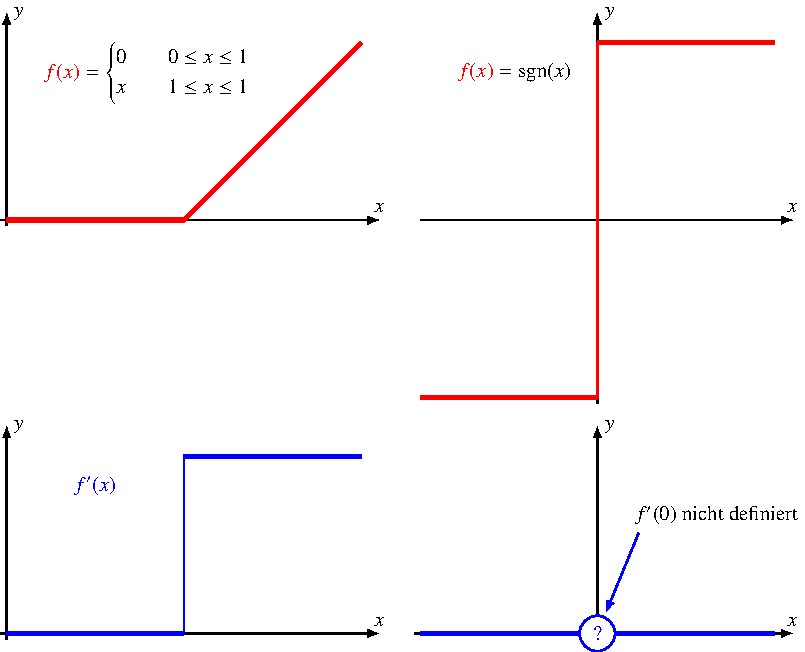
\includegraphics{chapters/010-skalarprodukt/images/schwach.pdf}
\caption{Schwache Ableitung einer nicht differenzierbaren Funktion.
Links die schwache Ableitung der Funktion von
Beispiel~\ref{buch:skalarprodukt:sobolevraum:bsp:schwachexistiert}.
Für die Signum-Funktion von
Beispiel~\ref{buch:skalarprodukt:sobolevraum:bsp:schwachexistiertnicht}
existiert die schwache Ableitung nicht, sie lässt für den Punkt $0$
nicht definieren.
\label{buch:skalarprodukt:sobolevraum:fig:schwach}}
\end{figure}
%
Die in Abbildung~\ref{buch:skalarprodukt:sobolevraum:fig:schwach} links
dargestellte Funktion
\[
f\colon (0,1) \to \mathbb{R}
:
x \mapsto
\begin{cases}
x&\qquad\text{für $0<x<1$}\\
1&\qquad\text{für $1\le x<2$}
\end{cases}
\]
ist stetig und integrierbar, aber sie ist an der Stelle $x=1$ nicht
differenzierbar.
Wir suchen die schwache Ableitung $v$ von $f$.

In einer Umgebung eines Punktes $x>1$ können wir Testfunktionen $\varphi$
so wählen, dass ihr Träger vollständig im Inneren des Intervals $(1,2)$
enthalten ist.
Mit diesen Testfunktionen können wir so rechnen, wie wenn $f$ die konstante
Funktion $1$ ist.
Das bedeutet für das Skalarprodukt
\[
\langle f,\varphi'\rangle
=
\int_1^2 \varphi'(x)\,dx
=
[\varphi(x)]_0^1 = 0.
\]
Das Skalarprodukt mit jeder beliebigen Testfunktion ist $0$, wir
müssen also $v(x)=0$ wählen.

Für $x$ im Teilinterval $(0,1)$ können wir die Testfunktionen so wählen,
dass der Träger vollständig im Inneren  von $(0,1)$ enthalten ist und
somit $f$ als die beliebig oft stetig differenzierbare Funktion $x$
behandelt werden darf.
Für das Skalarprodukt folgt dann
\[
-\langle f,\varphi'\rangle
=
-\int_0^1 f(x)\,\varphi'(x)\,dx
=
-\int_0^1 x\varphi'(x)\,dx
=
-[x\varphi(x)]_0^1 +\int_0^1 \varphi(x)\,dx
=
\langle 1,\varphi(x)\rangle,
\]
in diesem Teil des Intervals muss die schwache Ableitung den Wert $1$ 
haben.

Wir haben somit gefunden, dass die schwache Ableitung von $f$ die
Funktion
\[
v(x) = \begin{cases}
1&\qquad\text{für $0\le x<1$}
\\
0&\qquad\text{für $1< x<2$}
\end{cases}
\]
ist.
Wir kontrollieren dies, indem wir das Skalarprodukt für beliebige 
Testfunktionen $\varphi$ nachrechnen:
\begin{align*}
\langle v,\varphi\rangle
&=
\int_0^2 v(x)\,\varphi(x)\,dx
=
\int_0^1 1\,\varphi(x)\,dx
+
\int_1^2 0\,\varphi(x)\,dx.
\intertext{Jedes dieser Integrale kann man partiell integrieren:}
&=
[x\varphi(x)]_0^1 - \int_0^1 x\varphi'(x)\,dx
+
[1\varphi(x)]_1^2 - \int_1^2 1\varphi'(x)\,dx
\\
&=
\varphi(1) + \varphi(2) - \varphi(1) - \int_0^2 f(x)\,\varphi'(x)\,dx.
\intertext{Da $2$ ein Randpunkt ist, ist $\varphi(2)=0$, so dass sich}
&=-\langle f,\varphi'\rangle.
\end{align*}
ergibt.
Die Funktion $v$ ist also die schwache Ableitung von $f$.
\end{beispiel}

Eine Funktion in $W^{1,2}(\Omega)$ hat eine schwache Ableitung,
wie das Beispiel gezeigt hat, muss die Ableitung keine stetige
Funktion sein.
Ausserdem ist jede andere Funktion, die sich von der schwachen
Ableitung auf einer Menge vom Mass 0 unterscheidet, genauso eine
schwache Ableitung.
Trotzdem kann eine Funktion mit einer schwachen Ableitung nicht
beliebig ``wild'' sein, wie das folgende Beispiel zeigt.

\begin{beispiel}
\label{buch:skalarprodukt:sobolevraum:bsp:schwachexistiertnicht}
Die Signum-Funktion
\[
f\colon (-1,1) = \operatorname{sgn}(x) =
\begin{cases}
         - 1&\qquad\text{für $-1<x<0$}\\
\phantom{-}0&\qquad\text{für $x=0$}\\
\phantom{-}1&\qquad\text{für $0<x<1$}
\end{cases}
\]
ist nicht stetig (Abbildung~\ref{buch:skalarprodukt:sobolevraum:fig:schwach}).
$f$ ist fast überall konstant, in beiden Teilintervallen $(-1,0)$ und
$(0,1)$ ist die einzige mögliche schwache Ableitung von $f$ die
Nullfunktion.
Trotzdem kann $0$ nicht die schwache Ableitung von $f$ sein.
Wir wählen eine Testfunktion $\varphi$, die im Punkt $x=0$ von
Null verschieden ist.
Wäre $v$ eine schwache Ableitung von $f$, dann müsste
\begin{align*}
\langle v,\varphi\rangle
&=
-\langle f,\varphi'\rangle
=
-\int_{-1}^1 f(x) \varphi'(x)\,dx
\\
&=
-\int_{-1}^0 (-1)\cdot \varphi'(x)\,dx
-\int_{0}^1 1\cdot \varphi'(x)\,dx
=
\int_{-1}^0 \varphi'(x)\,dx
-
\int_{0}^1 \varphi'(x)\,dx
\\
&=
[\varphi(x)]_{-1}^0
-
[\varphi(x)]_{0}^1
=
\varphi(0)-\varphi(-1)
-
\varphi(1)+\varphi(0)
\\
&=
2\varphi(0)
\ne 0.
\end{align*}
Andererseits ist die Nullfunktion der einzige Kandidat für die
schwache Ableitun, für die das Skalarprodukt $\langle v,\varphi\rangle=0$
ist.
Dieser Widerspruch zeigt, dass die Funktion $f$ kein schwache
Ableitung hat.
\end{beispiel}

Die schwache Ableitung ermöglicht also mit gewissen Funktionen zu arbeiten,
die keine Ableitung im traditionellen Sinne haben.
Dank der Definition mit Hilfe eines Skalarproduktes in einem 
Hilbert-Raum darf man sich die Funktionen als Grenzwerte von
Cauchy-Folgen vorstellen.

%
% Physikalische Rechtfertigung
%
\subsection{Physikalische Rechtfertigung der schwachen Ableitung}
Die schwache Ableitung ersetzt die mit Hilfe eines Differenzenquotienten
definierte Änderungsrate durch eine Änderungsrate, die durch Vergleich
mit einer in der Umgebung eines Punktes konzentrierten Testfunktion
ermittelt wird.
Auf den ersten Blick mag das als Konzession an die Präzision der Ideen
der Analysis erscheinen, die Newton erfunden hat, um die Physik auf eine
neue Grundlage zu stellen.
Dabei wird aber vergessen, dass der Differenialquotient eine physikalisch
nicht erreichbare Idealisierung darstellt.
Keine Messung kann in einem Punkt im geometrischen Sinn erfolgen.
Die Bestimmung einer Position eines Massepunktes zum Beispiel erfolgt
durch Beobachtung des Lichtes, das vom Massepunkt reflektiert wird.
Doch der Massepunkt ist kein Punkt im geometrischen Sinn, er ist ausgedehnt
über ein endliches Gebiet.
Auch ist die Messung nicht instantan, es wird Licht gemessen, welches
über ein Zeitintervall vom Massepunkt reflektiert wird.
Das Messresultat entsteht also notwendigerweise als Mittelwert der
Beobachtung einer sehr grossen Zahl von Photonen, die von verschiedenen
Stellen reflektiert wurden.
Ein solcher Mittelwert ist genau das, was ein Skalarprodukt
$\langle f,\varphi\rangle$ mit einer Testfunktion ermittelt.

Die Feldgleichungen der Elektrodynamik wurden von Maxwell ausgehend
von Faradays Ideen als partielle Differentialgleichungen formuliert.
Sie verknüpfen die Werte des elektrischen Feldes $\vec{E}$ und des
magnetischen Feldes $\vec{B}$ mit der Ladungsdichte $\varrho$
und der Stromdichte $\vec{\jmath}$, die die Felder erzeugen.
Doch sowohl die Ladungsdichte wie auch die Stromdichte sind Idealisierungen.
Ladungen und Ströme sind nicht stetig über den Raum verteilt, sondern 
in Elektronen oder Atomkernen konzentriert.
Die Ladungsdichte entsteht daraus durch Messung der Ladung in einem kleine
Raumgebiet und Mittelung, was man wieder als Skalarprodukt mit einer
Testfunktion beschreiben kann.

Das elektrische Feld wird gemessen, indem die Kraft auf eine Testladung
im Feld ermittelt wird.
Ausser den prinzipiellen Einschränkungen an die Genauigkeit der
Positionsmessung wissen wir auch aus der Quantenmechanik, dass so etwas
wie die exakte Position eines Teilchens nicht gibt, wir können nur eine
Wahrscheinlichkeitsverteilung dafür bekommen.
Die Kraft äussert sich in einer Geschwindigkeitsänderung, die aber erst
messbar wird, wenn man die Beschleunigung eine gewisse Zeit lang aufrecht
erhält.
Das Messresultat ist also wieder ein Mittelwert über viele Positionen
und Zeitpunkte, oder anders ausgedrückt ein Skalarprodukt mit einer
Testfunktion.

Weitere Beispiele kann man auch in der Fluiddynamik finden.
Die Navier-Stokes-Gleichungen beschreiben die Strömung eines Mediums
unter der Annahme, dass es durch die Dichte $\varrho$ und die
Geschwindigkeit exakt beschreiben lässt.
Das Medium setzt sich aber aus einzelnen Atomen zusammen, die Dichte
ist also bereits ein Mittelwertbildung.
Bei der Geschwindigkeit wird das Problem noch deutlicher.
Auch die Strömungsgeschwindigkeit eines Gases ist der Mittelwert der
Strömungsgeschwindigkeit der Teilchen. 
Die Geschwindigkeit einzelner Teilchen ist dabei meistens sehr viel
grösser, nämlich im Bereich der Schallgeschwindigkeit, und äussert sich
in der Temperatur des Gases, also der mittleren kinetischen Energie.
Es ist nicht sinnvoll, von der Temperatur eines einzelnen Atoms zu
sprechen.

Alle diese Beispiele zeigen, dass die Ableitung als Änderungsrate, die
mit einem Differenzenquotienten bestimmt werden kann, eine Idealisierung
ist.
Wir können dies sogar etwas formeller zeigen.
Sei $x(t)$ die Koordinate eines Massepunktes zur Zeit $t$.
Die Messung kann nicht instantan erfolgen, im besten Fall ist die
gemessene Position ein Integral der Form
\[
\hat{x}(t)
=
\int_{-\infty}^\infty x(\tau) \varphi(\tau - t)\,d\tau.
\]
Darin ist $\varphi$ eine Testfunktion mit Träger in der Nähe von $0$.
Schreiben wir $T_t\varphi(\tau) = \varphi(\tau -t)$, dann können wir
das Messresultat auch als Skalarprodukt
$\hat{x}(t)=\langle x,T_t\varphi\rangle$
schreiben.
Die Messung mit der gleichen Aparatur einen Moment $\Delta t$ später ergibt
\[
\hat{x}(t+\Delta t)
=
\int_{-\infty}^\infty x(\tau) \varphi(\tau-t-\Delta t)\,dt
=
\langle x, T_{t+\Delta t}\varphi\rangle.
\]
Die Geschwindigkeit als Differenzenquotient ist
\begin{equation}
\frac{
\hat{x}(t+\Delta t)-\hat{x}(t)
}{\Delta t}
=
\frac{
\langle f,T_{t+\Delta t}\varphi\rangle
-
\langle f,T_{t}\varphi\rangle
}{
\Delta t
}
=
\left\langle
f,\frac{T_{t+\Delta t}\varphi - \varphi}{\Delta t}
\right\rangle
\label{buch:skalarprodukt:sobolevlraum:eqn:geschwindigkeit}
\end{equation}
Die Funktion $(T_{t+\Delta t}\varphi-T_t\varphi)/\Delta t$ ist eine 
beliebig oft stetig differenzierbare Funktion, die im Grenzwert
$\Delta t\to 0$ gegen
\[
\frac{
\varphi(\tau - t - \Delta t)
-
\varphi(\tau - t)
}{
\Delta t
}
=
-
\frac{
\varphi(\tau - t + \delta) - \varphi(\tau - t)
}{
\delta
}
\to 
-
\varphi'(\tau - t)
\quad
\text{für $\delta = - \Delta \to 0$}
\]
konvergiert.
Der Differenzenquotient
\eqref{buch:skalarprodukt:sobolevlraum:eqn:geschwindigkeit}
konvergiert daher gegen
\[
\lim_{\Delta t\to 0}
\frac{
\hat{x}(t+\Delta t)-\hat{x}(t)
}{\Delta t}
=
\left\langle
x,
\lim_{\Delta t\to 0}
\frac{T_{t+\Delta t}\varphi-T_t\varphi}{\Delta t}
\right\rangle
=
\langle f,-\varphi'\rangle
=
-
\langle f, \varphi'\rangle.
\]
Dieses einfache Modell einer ``unscharfen'' Messung führt also automatisch
auf das Konzept der schwachen Ableitung.








%\uebungsabschnitt
%\aufgabetoplevel{chapters/010-potenzen/uebungsaufgaben}
%\begin{uebungsaufgaben}
%\uebungsaufgabe{101}
%\uebungsaufgabe{102}
%\uebungsaufgabe{103}
%\uebungsaufgabe{104}
%\end{uebungsaufgaben}
%\endgroup


%
% chapter.tex -- Skalarprodukt
%
% (c) 2021 Prof Dr Andreas Müller, Hochschule Rapperswil
%
% !TeX spellcheck = de_CH
\chapter{Skalarprodukte
\label{buch:chapter:skalarprodukte}}
\kopflinks{Skalarprodukte}

%
% 1-definition.tex
%
% (c) 2023 Prof Dr Andreas Müller, OST Ostschweizer Fachhochschule
%
\section{Definition
\label{buch:opertoren:section:definition}}
\kopfrechts{Definition}


%
% 2-cauchyschwarz.tex
%
% (c) 2022 Prof Dr Andreas Müller, OST Ostschweizer Fachhochschule
%
\section{Ungleichungen
\label{buch:skalarprodukte:section:cauchyschwarz}}
\kopfrechts{Cauchy-Schwarz-Ungleichung}
In der Vektorgeometrie wird gelehrt, dass die Länge eines Vektors $u$
durch die Norm $\|u\|$ wiedergegeben wird und dass die geometrische
Intuition dazu passt.
Dazu gehört vor allem, dass die Dreiecksungleichung erfüllt ist,
dass also für drei Punkt $A$, $B$ und $C$
\begin{equation}
\overline{AB} \le \overline{AC} + \overline{BC}
\label{skalarprodukt:ungleichungen:eqn:dreieck}
\end{equation}
gilt.
In Vektorform bedeutet dies, dass
\[
\| b-a\|
\le
\| c-a\| + \|b-c\|.
\]
Schreibt man $u=c-a$ und $v=b-c$, dann ist $u+v=b-a$ und somit
\begin{equation}
\| u+v\| \le \|u\| + \|v\|.
\label{skalarprodukt:cauchyschwarz:eqn:dreieck0}
\end{equation}
Dies ist die Dreiecksungleichung in
Vektorform~\eqref{skalarprodukt:cauchyschwarz:eqn:dreieck0}.
Ziel dieses Abschnitts ist zu zeigen, dass jedes reelle oder
komplexe Skalarprodukt diese und weitere Eigenschaften automatisch
mitbringt.

%
% Cauchy-Schwarz-Ungleichung
%
\subsection{Cauchy-Schwarz-Ungleichung}
Sei also $\langle\;\,,\;\rangle$ ein reelles oder komplexes Skalarprodukt
auf dem Vektorraum $V$,
insbesondere ist $\langle v,v\rangle\ge 0$ für beliebige Vektoren $v\in V$.
Für zwei Vektoren $x,y\in V$ und $t\in \mathbb{R}$  gilt daher
\begin{align}
0
&\le
\| x+ty\|^2
=
\langle x+ty,x+ty\rangle
=
\langle x,x\rangle
+
t\langle x,y\rangle
+
t\langle y,x\rangle
+
t^2
\langle y,y\rangle.
\label{skalarprodukt:cauchyschwarz:eqn:quadrat}
\end{align}
Für ein reelles Skalarprodukt ist $\langle x,y\rangle=\langle y,x\rangle$
und damit
\begin{align}
0
&\le
\|x\|^2 + 2t\langle x,y\rangle + t^2 \|y\|^2.
\label{buch:skalarprodukt:cauchyschwarz:eqn:cspoly}
\end{align}
Dies ist ein quadratisches Polynom in der Variablen $t$, dessen Minimum
nicht negativ sein darf.

%
% Minimum eines quadratischen Polynoms
%
\subsubsection{Minimum eines quadratischen Polyoms}
Ein beliebiges quadratisches Polynom
\[
p(t)=at^2+bt+c
\]
kann durch
quadratisches Ergänzen in die Form
\[
p(t)
=
a\biggl(t+\frac{b}{2a}\biggr)^2 -\frac{b^2}{4a}+c
\]
gebracht werden.
Daraus kann man ablesen, dass das Minimum an der Stelle
\[
t_0
=
-\frac{b}{2a}
\]
angenommen wird und den Wert 
\begin{equation}
p(t_0)
=
c-\frac{b^2}{4a}
\end{equation}
hat.
Die gleiche Lösung kann natürlich auch durch Bestimmung des Minimums
von $p(t)$ mit Hilfe der Bedingung $p'(t_0)=0$ gefunden werden.

%
% Cauchy-Schwarz-Ungleichung für einen reellen Vektorraum
%
\subsubsection{Cauchy-Schwarz-Ungleichung für einen reellen Vektorraum}
Für~\eqref{buch:skalarprodukt:cauchyschwarz:eqn:cspoly}
ist
\[
a=\|y\|^2,\quad
b=2\langle x,y\rangle
\quad\text{und}\quad
c=\|x\|^2.
\]
Daher folgt aus~\eqref{buch:skalarprodukt:cauchyschwarz:eqn:cspoly}
\[
0
\le
\|x\|^2 - \frac{\langle x,y\rangle^2}{\|y\|^2}
\qquad\Rightarrow\qquad
\langle x,y\rangle^2 \le \|x\|^2\, \|y\|^2
\qquad\Rightarrow\qquad
|\langle x,y\rangle| \le \|x\|\, \|y\|.
\]
Dies ist die Cauchy-Schwarz-Ungleichung für das Skalarprodukt
$\langle \;\,,\;\rangle$.

\begin{satz}[Cauchy-Schwarz]
\label{buch:skalarprodukt:cauchy-schwarz:satz:reell}
Ein reelles Skalarprodukt $\langle\;\,,\;\rangle$ auf dem reellen Vektorraum
$V$ erfüllt die Cauchy-Schwarz-Ungleichung
\[
|\langle x, y\rangle| \le \|x\|\,\|y\|
\]
für $x,y\in V$.
\end{satz}

%
% Cauchy-Schwarz-Ungleichung für einen komplexen Vektorraum
%
\subsubsection{Cauchy-Schwarz-Ungleichung für einen komplexen Vektorraum}
Für ein komplexes Skalarprodukt ist das Produkt $\langle x,y\rangle$
nicht mehr unbedingt reell und kann damit nicht mehr direkt mit den
Normen $\|x\|^2u$ und $\|y\|^2$ vergleichen.
Wir ersetzen daher $t$ durch
$t\langle y,x\rangle=t\overline{\langle x,y\rangle}$
und erhalten 
\begin{align*}
0
\le
\|x+t\langle y,x\rangle y\|^2
&=
\langle x,x\rangle
+t\langle y,x\rangle \langle x,y\rangle
+t\overline{\langle y,x\rangle}\langle y,x\rangle
+t^2\langle y,y\rangle
\\
&=
\|x\|^2
+
t
2|\langle x,y\rangle|^2
+
t^2 |\langle x,y\rangle|^2
\|y\|^2.
\end{align*}
Dies ist wieder ein quadratisches Polynom, diesmal mit den Koeffizienten
\[
a= |\langle x,y\rangle|^2 \|y\|^2,
\quad
b= 2|\langle x,y\rangle|^2
\quad\text{und}\quad
c= \|x\|^2.
\]
Das Minimum dieses Polynoms ist nach
\[
0
\le
c-\frac{b^2}{4a}
=
\|x\|^2 - \frac{|\langle x,y\rangle|^4}{|\langle x,y\rangle|^2\,\|y\|^2}
=
\|x\|^2 - \frac{|\langle x,y\rangle|^2}{\|y\|^2}
\quad\Rightarrow\quad
|\langle x,y\rangle|^2 \le \|x\|^2\,\|y\|^2
\quad\Rightarrow\quad
|\langle x,y\rangle \le \|x\|\,\|y\|.
\]
Dies ist die Cauchy-Schwarz-Ungleichung für einen komplexen Vektorraum.

\begin{satz}[Cauchy-Satz]
\label{buch:skalarprodukt:cauchy-schwarz:satz:komplex}
Ein komplexes Skalarprodukt $\langle\;\,,\;\rangle$ auf dem komplexen Vektorraum
$V$ erfüllt die Cauchy-Schwarz-Ungleichung
\[
|\langle x, y\rangle| \le \|x\|\,\|y\|
\]
für $x,y\in V$.
\end{satz}

Man beachte, dass die
Sätze~\ref{buch:skalarprodukt:cauchy-schwarz:satz:reell}
und
\ref{buch:skalarprodukt:cauchy-schwarz:satz:komplex}
nur die Axiome eines Skalarproduktes verwenden.
Sie gelten also
ganz unabhängig von der konkreten Definition des Skalarproduktes,
solange die Eigenschaften eines Skalarproduktes gegeben sind.

\begin{beispiel}
Die sesquilineare Funktion
\[
\langle x,y\rangle
=
\sum_{i=1}^n\overline{x}_i y_i
\]
für Vektoren $x,y\in\mathbb{C}^n$ ist positiv definit, denn
\[
\langle x,x\rangle
=
\sum_{i=1}^n \overline{x}_i x_i = \sum_{i=1}^n |x_i|^2 > 0
\]
für $x\ne 0$.
Nach Satz~\ref{buch:skalarprodukt:cauchy-schwarz:satz:komplex}
gilt daher
\[
\biggl|
\sum_{i=1}^n \overline{x}_i y_i
\biggr|
\le
\sqrt{\sum_{i=1}^n |x_i|^2} \sqrt{\sum_{i=1}^n |y_i|^2}
\quad\text{oder auch}\quad
\biggl|
\sum_{i=1}^n x_i y_i
\biggr|
\le
\sqrt{\sum_{i=1}^n |x_i|^2} \sqrt{\sum_{i=1}^n |y_i|^2}
\]
für beliebige Vektoren $x,y\in\mathbb{C}^n$.
\end{beispiel}

\begin{beispiel}
Die sesquilineare Funktion
\[
\langle f,g\rangle
=
\int_a^b \overline{f(x)} g(x)\,dx
\]
für komplexwertige, stetige Funktion auf dem Intervall $[a,b]$
ist positiv definit, denn
\[
\langle f,f\rangle
=
\int_a^b \overline{f(x)} f(x)\,dx
=
\int_a^b |f(x)|^2\,dx
\ge 0
\]
für $f\ne 0$.
Nach Satz~\ref{buch:skalarprodukt:cauchy-schwarz:satz:komplex}
gilt daher
\begin{align*}
\biggl|\int_a^b \overline{f(x)}g(x)\,dx\biggr|
&\le
\sqrt{\int_a^b |f(x)|^2\,dx}
\sqrt{\int_a^b |g(x)|^2\,dx}
\intertext{oder auch}
\biggl|\int_a^b f(x) g(x)\,dx\biggr|
&\le
\sqrt{\int_a^b |f(x)|^2\,dx}
\sqrt{\int_a^b |g(x)|^2\,dx}
\end{align*}
für beliebige komplexwertige stetige Funktionen $f,g$ auf dem
Intervall $[a,b]$.
\end{beispiel}

%
% Dreiecksungleichung
%
\subsection{Dreiecksungleichung}
Die Intuition einer Längenmessung basiert auf der
Dreiecksungleichung~\eqref{skalarprodukt:ungleichungen:eqn:dreieck}.
Sie ist gleichbedeutend mit der
Vektorform~\eqref{skalarprodukt:cauchyschwarz:eqn:dreieck0}
der Ungleichung.

Die Cauchy-Schwarz-Ungleichung ermöglicht nun, diese Ungleichung
nachzurechnen.
Die Norm von $\|x+y\|^2$ ist
\[
\|x+y\|^2
=
\langle x+y,x+y\rangle
=
\langle x,x\rangle
+
\langle x,y\rangle
+
\langle y,x\rangle
+
\langle y,y\rangle
=
\|x\|^2 + 2\operatorname{Re}\langle x,y\rangle + \|y\|^2.
\]
Den mittleren Term kann man mit der Cauchy-Schwarz-Ungleichung
umformen:
\begin{align*}
\|x\|^2 + 2\operatorname{Re}\langle x,y\rangle + \|y\|^2.
&\le
\|x\|^2 + 2|\operatorname{Re}\langle x,y\rangle| + \|y\|^2.
\\
&\le
\|x\|^2 + 2|\langle x,y\rangle| + \|y\|^2.
\\
&\le
\|x\|^2 + 2\|x\|\,\|y\| + \|y\|^2
=
(\|x\| + \|y\|)^2.
\end{align*}
Durch Ziehen der Wurzel folgt
\[
\|x+y\| \le \|x\| + \|y\|.
\]
Damit ist der folgende Satz bewiesen.

\begin{satz}[Dreiecksungleichung]
Für die Norm zu einem beliebigen Skalarprodukt auf dem reellen
oder komplexen Vektorraum $V$ gilt die Dreiecksungleichung
\[
\|x+y\| \le \|x\| + \|y\|
\]
für $x,y\in V$.
\end{satz}

%
% Normen
%
\subsection{Normen
\label{skalarprodukt:cauchyschwarz:subsection:norm}}
Das Skalarprodukt ist nicht die einzige Möglichkeit, eine Norm auf
einem Vektorraum zu definieren.
Zum Beispiel kann man auf $\mathbb{C}^n$ die sogenannte $l^1$-Norm
definieren.

\begin{definition}
Die Funktion
\[
\|x\|_1
=
\sum_{i=1}^n |x_i|
\]
für $x\in\mathbb{C}^n$ heisst die {\em $l^1$-Norm} auf $\mathbb{C}^n$.
\end{definition}

Die Funktion $\|\cdot\|_1$ ist eine Norm im Sinne der folgenden Definition.

\begin{definition}
Eine Funktion $\|\cdot\| \colon V\to\mathbb{R}$ auf einem reellen
oder komplexen Vektorraum $V$ heisst eine {\em Norm}, wenn Sie die
folgenden Bedingungen erfüllt
\begin{enumerate}
\item
$\|\lambda x\| = |\lambda|\, \|x\|$ für $x\in V$ und $\lambda\in \Bbbk$
\item
Für alle Vektoren $x\in V$ mit $x\ne 0$ gilt $\|x\|>0$.
\item
Dreiecksungleichung: $\|x+y\| \le \|x\| + \|y\|$ für alle $x,y\in V$
\end{enumerate}
\end{definition}

Es ist klar, dass die $l^1$-Norm die Bedingungen~1 und 2 erfüllt.
Aber auch die Bedingung~3 kann man leicht  nachprüfen:
\[
\|x+y\|_1
=
\sum_{i=1}^n |(x+y)_i|
=
\sum_{i=1}^n |x_i+y_i|
\le
\sum_{i=1}^n(|x_i|+|y_i|)
=
\sum_{i=1}^n|x_i|
+
\sum_{i=1}^n|y_i|
=
\|x\|_1 + \|y\|_1,
\]
wozu wir nur die Dreiecksungleichung $|a+b|\le |a| + |b|$ für reelle 
oder komplexe Zahlen $a,b$ benötigen.

\begin{beispiel}
Die Funktion
\[
\|x\|_\infty = \sup_{1\le i\le n} |x_i|
\]
ist eine Norm auf $\mathbb{C}^n$.
\end{beispiel}

Auch in diesem Fall sind die Bedingungen~1 und 2 ganz offensichtlich erfüllt.
Für die Dreiecksungleichung rechnen
\begin{align*}
\|x+y\|_\infty
&=
\sup_{1\le i\le n} |x_i+y_i|
\le
\sup_{1\le i\le n} (|x_i|+|y_i|)
\le
\sup_{1\le i\le n} |x_i|+\sup_{1\le i\le n}|y_i|
=
\|x\|_\infty + \|y\|_\infty.
\end{align*}
Somit ist $\|\cdot\|_\infty$ eine Norm auf $\mathbb{C}^n$.

%
% Polaridentität
%
\subsection{Polaridentität}
Die durch das Skalarprodukt definierte Norm
\( \|x\|^2=\langle x,x\rangle \)
ist nach Abschnitt~\ref{skalarprodukt:cauchyschwarz:subsection:norm}
ein Spezialfall einer Norm.
Ist es möglich, für eine Norm, die von einem Skalarprodukt herkommt,
das Skalarprodukt wieder zu rekonstruieren?

%
% Reelles Skalarprodukt aus der Norm
%
\subsubsection{Reelles Skalarprodukt aus der Norm}
Die Antwort gibt der folgende Satz.

\begin{satz}[Polaridentität]
\label{skalarprodukt:cauchyschwarz:satz:polarformel}
Ist $\|\cdot\|$ die Norm zu einem Skalarprodukt auf dem reellen Vektorraum
$V$, dann kann das Skalarprodukt zweier Vektoren $x,y\in V$ mittels
der sogenannten {\em Polaridentität}
\index{Polaridentität}%
\begin{equation}
\langle x, y\rangle
=
\frac12\bigl(
\|x+y\|^2 - \|x\|^2 - \|y\|^2 
\bigr)
\label{skalarprodukt:cauchyschwarz:eqn:polar}
\end{equation}
berechnet werden.
\end{satz}

\begin{proof}[Beweis]
Die Gleichung
\begin{align*}
\|x+y\|^2
&=
\langle x+y,x+y\rangle
=
\|x\|^2 + 2\langle x,y\rangle + \|y\|^2 
\end{align*}
kann nach $\langle x,y\rangle$ aufgelöst werden und ergibt
die behauptete Formel~\eqref{skalarprodukt:cauchyschwarz:eqn:polar}.
\end{proof}

% 
% Parallelogrammgleichung
%
\subsubsection{Parallelogrammgleichung}
\begin{figure}
\centering
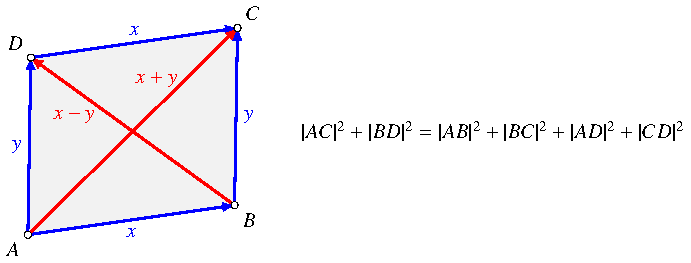
\includegraphics{chapters/010-skalarprodukt/images/parallelogramm.pdf}
\caption{Parallelogrammregel für eine Norm, die aus einem Skalarprodukt
entsteht.
\label{skalarprodukt:cauchyschwarz:fig:parallelogramm}}
\end{figure}
Die Polaridentitäten können auch noch in einer anderen Form geschrieben
werden.
Dazu berechnet man zusätzlich die Norm von $x-y$:
\begin{align*}
\|x+y\|^2
&=
\|x\|^2 + \|y\|^2 + 2\langle x, y\rangle
\\
\|x-y\|^2
&=
\|x\|^2 + \|y\|^2 - 2\langle x, y\rangle
\\
\|x+y\|^2 +\|x-y\|^2
&=
2\|x\|^2 + 2\|y\|^2
\end{align*}

\begin{satz}
\label{skalarprodukt:cauchyschwarz:satz:parallelgramm}
Für eine Norm, die von einem reellen Skalarprodukt herkommt, gilt die
Parallelogrammformel
\begin{equation}
\|x+y\|^2 +\|x-y\|^2
=
2\|x\|^2 + 2\|y\|^2.
\label{skalarprodukt:cauchyschwarz:eqn:parallelgramm}
\end{equation}
(Abbildung~\ref{skalarprodukt:cauchyschwarz:fig:parallelogramm})
\end{satz}

Das Skalarprodukt kann man damit auf verschiedene Weise aus der
Norm gewinnen:
\begin{equation}
\begin{aligned}
\langle x, y\rangle
&=
{\textstyle\frac12}\bigl( \|x\|^2 + \|y\|^2 - \|x+y\|^2 \bigr)
\\
&=
{\textstyle\frac12}\bigl(
\|x+y\|^2
-
\|x\|^2 
-
\|y\|^2
\bigr)
\\
&=
{\textstyle\frac14}\bigl(
\|x+y\|^2 - \|x-y\|^2
\bigr).
\end{aligned}
\label{skalarprodukt:cauchyschwarz:eqn:realteil}
\end{equation}
Nur die letzte Formel ist noch nicht gut begründet.
Man kann aber sofort nachrechnen, dass 
\begin{align*}
\|x+y\|^2&=\|x\|^2+2\langle x,y\rangle+\|y\|^2\\
\|x-y\|^2&=\|x\|^2-2\langle x,y\rangle+\|y\|^2
\intertext{die Differenz}
\|x+y\|^2 - \|x-y\|^2 &= 4\langle x,y\rangle
\qquad
\Rightarrow
\qquad
\langle x,y\rangle
=
\frac14\bigl(\|x+y\|^2 - \|x-y\|^2\bigr)
\end{align*}
haben.

%
% Komplexes Parallelogramm aus der Norm
%
\subsubsection{Komplexe Skalarprodukt}
Das Resultat von Satz~\ref{skalarprodukt:cauchyschwarz:satz:polarformel}
gilt in abgeänderter Form auch für komplexe Skalarprodukte.
Da das Skalarprodukt auch einen nichtverschwindenen Imaginärteil haben
kann, wird eine zusätzliche Gleichung zur Berechnung des Imaginärteils
nötig.
Eine solche kann gewonnen werden, indem zusätzlich die Normen
$\|x+iy\|^2$ und $\|x-iy\|^2$ berechnet werden.
Dazu ist zu beachten, dass
\[
\langle x,y\rangle
-
\langle y,x\rangle
=
\langle x,y\rangle
-
\overline{
\langle x,y\rangle
}
=
2i\operatorname{Im}\langle x,y\rangle
\]
Damit erhält man
\begin{align*}
\|x+iy\|^2 &= \|x\|^2 + i\langle x,y\rangle - i\langle y,x\rangle + \|y\|^2 
           = \|x\|^2 + 2\operatorname{Im}\langle x,y\rangle + \|y\|^2 \\
\|x-iy\|^2 &= \|x\|^2 - i\langle x,y\rangle + i\langle y,x\rangle + \|y\|^2 
           = \|x\|^2 - 2\operatorname{Im}\langle x,y\rangle + \|y\|^2.
\end{align*}
Damit kann man nach dem Imaginärteil des Skalarproduktes auflösen und
die Formeln
finden, die den Formeln
\eqref{skalarprodukt:cauchyschwarz:eqn:realteil}
für das reelle Skalarprodukt entsprechen.
\eqref{skalarprodukt:cauchyschwarz:eqn:realteil}
Formeln bleiben gültig als Formeln für den Realteil des Skalarproduktes.
Damit haben wir den folgenden Satz gefunden.

\begin{satz}[Polaridentitäten für ein komplexes Skalarprodukt]
Ist $\|\cdot\|$ die Norm, die aus dem komplexen Skalarprodukt
$\langle\;\,,\;\rangle$ auf einem Vektorraum $V$ gewonnen wurde,
dann können Real- und Imaginärteil mit den Formeln
\begin{align*}
\operatorname{Re}\langle x,y\rangle
&=
{\textstyle\frac12}\bigl(
\|x+y\|^2 - \|x\|^2 -\|y\|^2
\bigr)
\\
&=
{\textstyle\frac12}\bigl(
\|x\|^2 +\|y\|^2 - \|x+y\|^2
\bigr)
\\
&=
{\textstyle\frac14}\bigl(
\|x+y\|^2 - \|x-y\|^2
\bigr),
\\
\operatorname{Im}\langle x,y\rangle
&=
{\textstyle\frac12}\bigl(
\|x+iy\|^2-\|x\|^2-\|y\|^2
\bigr)
\\
&=
{\textstyle\frac12}\bigl(
\|x\|^2+\|y\|^2-\|x-iy\|^2
\bigr)
\\
&=
{\textstyle\frac14}\bigl(
\|x+iy\|^2
-
\|x-iy\|^2
\bigr)
\end{align*}
für beliebige Vektoren $x,y\in V$
allein aus Werten der Norm berechnet werden.
\end{satz}


%
% 3-funktionenraeume.tex
%
% (c) 2022 Prof Dr Andreas Müller, OST Ostschweizer Fachhochschule
%
\section{Funktionenräume
\label{buch:skalarprodukt:section:funktionenraeume}}
\kopfrechts{Funktionenräume}
Ziel der harmonischen Analysis ist die effiziente Approximation einer
grossen Klasse von Funktionen.
Als approximierende Funktionen kommen stetige Funktionen, Polynome,
trigonometrische Polynome oder eine ähnlich, einfach konstruierbare
Funktionenfamilie in Frage.
Es gilt zunächst herauszufinden, was ``Approximation'' genau heissen
soll und von welchen Funktionen man überhaupt erwarten kann, dass sie
approximiert werden können.

%
% Stetige Funktionen
%
\subsection{Stetige Funktionen
\label{buch:skalarprodukt:subsection:stetige-funktionen}}
Der frühe intuitive Funktionsbegriff ging oft von der Vorstellung einer
in einem Strich gezeichneten Kurve aus, wie man sie von den Graphen
der Polynome oder der trigonometrischen Funktionen her kennt.
In moderner Sprechweise sind dies die stetigen Funktionen.

\begin{definition}
Eine Funktion $f\colon I\to\mathbb{R}$ mit $I\subset \mathbb{R}$
heisst stetig in einem Punkt $x_0\in I$, wenn für jedes $\varepsilon>0$
ein $\delta>0$ existiert derart, dass $f(x)-f(x_0)|<\delta$ sobald
$|x-x_0|<\varepsilon$.
\end{definition}

Nur die Eigenschaft, eine Abstandsmessung zu besitzen, wird vom
Definitionsbereich $I\subset \mathbb{R}$ verlangt.
Der Stetigkeitsbegriff kann daher verallgemeinert werden auf den
Begriff des metrischen Raumes.

\begin{definition}
Eine {\em Metrik} auf einer Menge $X$ ist eine Funktion
\index{Metrik}%
$d\colon X\times X\to \mathbb{R}$
mit den folgenden Eigenschaften
\begin{enumerate}
\item
Positiv definit: $d(x,y)\ge 0$ und $d(x,y)$ genau dann, wenn $x=y$.
\item
Symmetrie: \(d(x,y)=d(y,x)\)
\item
Dreiecksungleichung: \( d(x,y) \le d(x,z) + d(z,y) \).
\end{enumerate}
Ein {\em metrischer Raum} ist ein Menge $X$ mit einer Metrik.
\index{matrischer Raum}%
\end{definition}

In einem metrischen Raum ist der Begriff des Grenzwertes übertragbar.
Mit dem Begriff des Grenzwertes lässt sich auch der Begriff der
Stetigkeit verallgemeinern.

\begin{definition}
Ist $x_n\in X$ eine Folge von Punkten in einem metrischen Raum $X$,
dann heisst $x$ der Grenzwert der Folge $x_n$, wenn es für jedes
$\varepsilon>0$ ein $N>0$ gibt derhart, dass
$d(x_n,x)\le \varepsilon$ für alle $n>N$.
Eine Funktion $f\colon X\to Y$ zwischen metrischen Räumen heisst
stetig im Punkt $x\in X$, wenn für jede Folge $x_n\in X$ mit
Grenzwert $x$ auch die Folge $y_n=f(x_n)\in Y$ konvergiert und
den Grenzwert $y=f(x)$ hat.
\end{definition}

Teilmengen von $\mathbb{R}$ oder $\mathbb{R}^n$ tragen natürlich
die Struktur eines metrischen Raumes mit der Abstandsmessung in 
$\mathbb{R}^n$ als Metrik
\[
d(x,y) = \sqrt{(x_1-y_1)^2 + \ldots + (x_n-y_n)^2} = \|x-y\|.
\]
Die Eigenschaften einer Metrik wurden bereits in Abschnitt
\ref{buch:skalarprodukte:section:cauchyschwarz} nachgewiesen.

Der Begriff des Grenzwertes klärt, was mit der Approximation von $x$
durch eine Folge $x_n$ gemeint ist.
Wenn man darauf aufbauend die Konvergenz einer Folge von Funktionen
gegen eine Grenzfunktion definieren will, braucht man einen Abstansbegriff
zwischen Funktionen.
Ein erster Versuch könnte sein, als Abstand zwischen zwei Funktionen
$f$ und $g$ die Funktion
\[
d(f,g) = |f(x_0) - g(x_0)|.
\]
Die Menge der Funktionen wird dadurch jedoch nicht zu einem metrischen
Raum.
Zwar gilt sicher die Symmetrie und Dreiecksungleichung, und auch 
$d(f,g)\ge 0$ für beliebige Funktionen.
Aber wenn $d(f,g)=0$ ist, heisst das nur, dass $f$ und $g$ im Punkt
$x_0$ den gleichen Wert haben.
Ausser in trivialen Fällen wird es Funktionen geben, die zwar im Punkt
$x_0$ übereinstimmen, sich aber in mindestens einem anderen Punkt
unterscheiden.

%
% Normierte Räume
%
\subsubsection{Normierte Räume}
Die stetigen Funktionen bilden aber keine strukturlose Menge, sie
bilden einen Vektorraum: die Summe von stetigen Funktionen ist ebenfalls
stetig, multiplizieren einer stetigen Funktion mit einem Skalar führt
nicht aus der Menge der stetigen Funktionen heraus.
Die für den Grenzwertbegriff von Funktionen verwendete Abstandsmessung 
sollte der Vektorraumstruktur ebenfalls Rechnung tragen.

\begin{definition}
\label{buch:skalaprodukt:funktionenraume:def:norm}
Sei $V$ ein Vektorraum über $\mathbb{R}$, dann heisst eine Funktion
\( \|\;\cdot\;\| \colon V \to \mathbb{R}\) eine {\em Norm}, wenn gilt
\index{Norm}
\begin{enumerate}
\item
Definit: $ \|x\| = 0 \Rightarrow x=0$
\item
Homogeneität: $ \| \lambda x \| = |\lambda| \cdot \|x\|$
\item
Dreiecksungleichung: $\|x+y\| \le \|x\| + \|y\|$
\end{enumerate}
Ein {\em normierter Raum} ist ein Vektorraum $V$ mit einer Norm.
\end{definition}

%
% Vollständigkeit
%
\subsubsection{Vollständigkeit}
In den rationalen Zahlen hat nicht jede Folge einen Grenzwert.
Die Zahl $\sqrt{2}$ lässt sich beliebig genau durch rationale Zahlen
approximieren, sie ist aber nicht in $\mathbb{Q}$.
Ähnlich lässt sich die Funktion $x\mapsto \sqrt{x}$ beliebig genau 
durch Polyome approximieren, sie ist aber selbst kein Poylnome

\begin{definition}
Ein Folge $x_n\in X$ in einem metrischen Raum heisst {\em Cauchy-Folge},
wenn es für jedes $\varepsilon>0$ ein $N>0$ gibt derart, dass 
$|x_n-x_m|<\varepsilon$ wenn $n,m>N$ ist.
\end{definition}

Cauchy-Folgen sind also Folgen, die sich für genügend grossen Index
kaum mehr ändern und für die man daher Konvergenz erwarten würde.

\begin{definition}
Ein normierter Raum heisst {\em vollständig} oder ein Banach-Raum,
wenn jede Cauchy-Folge einen Grenzwert hat.
\end{definition}

Die rationalen Zahlen $\mathbb{Q}$ bilden keinen vollständigen
metrischen Raum, aber die reellen Zahlen $\mathbb{R}$ enthalten
alle Grenzwerte von Cauchy-Folgen, $\mathbb{R}$ ist eine vollständiger
metrischer Raum.
Die Menge der Polynome, betrachtet als Teilmenge der Menge der
stetigen Funktionen $[0,1]\to\mathbb{R}$ ist nicht vollständig,
da es eine Folge $f_n(x)$ von Approximationsfunktionen der Funktion
$x\mapsto \sqrt{x}$ gibt.
Als Cauchy-Folge konvergiert sie zwar gegen eine stetige Funktion,
aber die Grenzfunktion ist nicht mehr im Raum der Polynome.

Das Ziel der folgenden Kapitel ist also, zu geeignet interessanten
Funktionenfamilien ``gute'' Normen zu finden derart, dass Cauchy-Folgen
konvergieren gegen Funktionen, die immer noch ausreichend viele
nützliche Eigenschaften haben.
Im besten Fall konvergieren stetige Funktionen gegen stetige Funktionen,
es wird sich aber zeigen, dass diese Anforderung zu streng ist.

%
% Norm fpr stetige Funktionen
%
\subsection{Norm für stetige Funktionen
\label{buch:skalarprodukt:subsection:normfuerstetigefunktionen}}
Damit man von Konvergenz von Folgen stetiger Funktionen sprechen kann,
brauchen wir jetzt also eine Norm für stetige Funktionen.

\begin{definition}
Sei $X$ ein metrischer Raum und
\[
C(X)
=
C_{\mathbb{R}}(X)
=
\{
f\colon X \to\mathbb{R}\mid
\text{$f$ ist stetig}
\}
\]
der Vektorraum der stetigen Funktion auf $X$.
Die Norm von $C(X)$ ist definiert als
\[
\|f\| = \sup_{x\in X} |f(x)|.
\]
Sie heisst die {\em Supremum-Norm}.
\end{definition}

Wir prüfen nach, dass die Supremum-Norm tatsächlich eine Norm ist.
Dazu sind die definierenden Eigenschaften nachzurechnen:
\begin{enumerate}
\item Definit: 
\[
0
=
\|f\|
=
\sup_{x\in X} |f(x)|
\quad\Rightarrow\quad
f(x)=0 \;\forall x\in X
\quad\Rightarrow\quad
f\in C(X).
\]
\item Homogeneität:
\[
\|\lambda f\|
=
\sup_{x\in X} |\lambda f(x)|
=
|\lambda| \sup_{x\in X} |f(x)|
=
|\lambda| \cdot \|f\|.
\]
\item
Dreiecksungleichung:
\[
\|f+g\|
=
\sup_{x\in X}|f(x)+g(x)|
\le
\sup_{x\in X}(|f(x)|+|g(x)|)
\le
\sup_{x\in X}|f(x)|+\sup_{x\in X}|g(x)|
=
\|f\| + \|g\|.
\]
\end{enumerate}

Eine Cauchy-Folge $f_n$ von Funktionen $X\to \mathbb{R}$ hat die
Eigenschaft, dass für jedes $\varepsilon >0$ ein $N>0$ existiert,
derart dass $\|f_n-f_m\|<\varepsilon$ ist.
Da die Norm der maximale Unterschied von Funktionswerten ist,
folgt dass für eine Cauchy-Folge in $C(X)$ die Folge $f_n(x)$ eine
Cauchy-Folge in $\mathbb{R}$ ist und damit einen Grenzwert in $\mathbb{R}$
hat.
Die Funktion $f(x) = \lim_{n\to\infty}f_n(x)$ ist die Grenzfunktion.
Die Konvergenz bezüglich der Norm besagt, dass für jedes $\varepsilon>0$
es ein $N>0$ gibt derart, dass
\[
\varepsilon 
>
\|f_n-f\|
\ge 
|f_n(x)-f(x)|
\]
ist für alle $n>N$ und unabhängig von $x\in X$.
Die Konvergenz bezüglich der $\|\;\cdot\;\|$-Norm ist also die wohlbekannte
gleichmässige Konvergenz.
Es kann gezeigt werden, dass die Grenzfunktion wieder stetig ist.

\begin{satz}
Der Raum der stetigen Funktion $C(X)$ mit der Supremumg-Norm ist
ein Banach-Raum.
\end{satz}

%
% Skalarprodukt
%
\subsection{Skalarprodukt
\label{buch:skalarprodukt:subsection:skalarprodukt}}
\begin{figure}
\centering
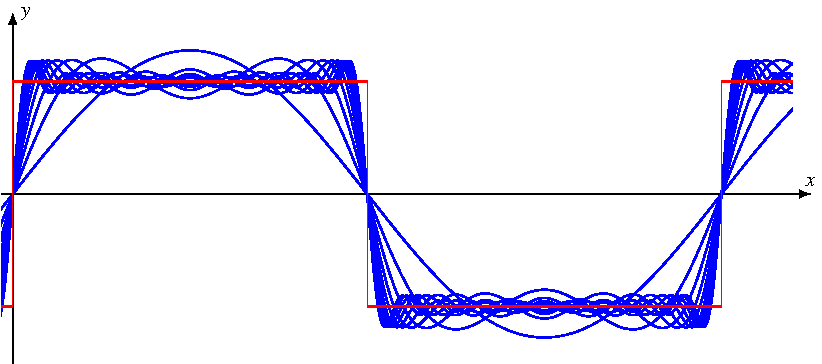
\includegraphics{chapters/010-skalarprodukt/images/fourierrechteck.pdf}
\caption{Approximation der Rechteckfunktion (rot) durch eine Folge
von Partialsummen der Fourier-Reihe.
\label{buch:skalarprodukt:fig:fourierrechteck}}
\end{figure}%
Die Supremum-Norm auf dem Raum der stetigen Funktionen hat den
Begriff der gleichmässig konvergenten Funktionenfolgen ergeben.
Cauchy-Folgen von stetigen Funktionen in der Supremum-Norm konvergieren
wieder gegen eine stetige Funktione.
Ist eine Funktion nicht stetig, lässt Sie sich im Sinne der Supremum-Norm
nicht durch stetige Funktionen approximieren.
Andererseits hat Fourier gezeigt, wie man technische wichtige Funktionen
wie die Rechteckfunktion durch trigonometrische Polynome
\begin{equation}
f_n(x)
=
\frac{4}{\pi} \sum_{k=0}^n \frac{\sin kx}{k}
=
\frac{4}{\pi} \biggl(
\sin x
+
\frac{\sin 3x}{3}
+
\frac{\sin 5x}{5}
+
\frac{\sin 7x}{7}
+
\ldots
\biggr)
\label{buch:skalarprodukt:eqn:rechteckreihe}
\end{equation}
approximieren kann.
Diese sind alle stetig und kommen der Rechteckfunktion in jedem Punkt,
in dem die Funktion stetig ist, beliebig nahe.
An den Stellen $x = n\pi$ hat die Grenzfunktion eine Sprungstelle,
die approximierenden Funktionen haben dort immer Abstand $1$
(siehe Abbildung~\ref{buch:skalarprodukt:fig:fourierrechteck}).
Die Folge ist also keine Cauchy-Folge und sie konvergiert nicht im
Sinne der Supremum-Norm.
Für solche Anwendungen muss eine besser geeignete Norm gefunden werden,
in der die Folge konvergiert.

%
% Skalarprodukt von Funktion
%
\subsubsection{Die $L^1$-Norm einer Funktion}
Die Supremum-Norm sieht nur den grössten Wert, die Konvergenz der Folge
\eqref{buch:skalarprodukt:eqn:rechteckreihe} ist aber nicht gleichmässig,
die maximale Abweichung ist immer $1$.
Gesucht ist eine Norm, die für die Folge
\eqref{buch:skalarprodukt:eqn:rechteckreihe} 
nur im Mittel eine Abweichung feststellt.
Für die Berechnung des Mittelwerts kann das Integral verwendet werden:

\begin{definition}
\label{buch:skalaprodukt:definition:l1norm}
Für eine stetige Funktion $X\to\mathbb{R}$, für die $x\mapsto |f(x)|$
integrierbar ist, heisst
\begin{equation}
\|f\|_1 = \int_X |f(x)|\,dx
\label{buch:skalarprodukt:eqn:l1norm}
\end{equation}
die {\em $L^1$-Norm} der Funktion $f$.
\end{definition}

Die $L^1$-Norm ist tatsächlich eine Norm, wir verifizieren die
definierenden Eigenschaften einer Norm.
\begin{enumerate}
\item
Definit: Sei $f$ eine stetige Funktion mit $\|f\|_1=0$
Wäre $f\ne 0$, dann gäbe es einen Punkt $x_0\in X$ mit $f(x_0) \ne 0$.
Da $f$ stetig ist, ist $f|(x)| > \frac12|f(x_0)|$ für $x$ in einer
$\delta$-Umgebung von $x_0$.
Dann folgt für die $L^1$-Norm
\begin{align*}
\|f\|_1
=
\int_X |f(x)|\,dx
\ge
\frac12 |f(x_0)| \cdot \delta 
> 0.
\end{align*}
Dies widerspricht der Annahme, dass $\|f\|_1=0$ ist, also muss $f=0$ sein.
\item
Homogeneität folgt durch direkte Rechnung
\[
\|\lambda f\|_1
=
\int_X |\lambda f(x)|\,dx
=
|\lambda|
\int_X |f(x)|\,dx
=
|\lambda| \cdot \|f\|.
\]
\item
Die Dreiecksungleichung folgt aus
\[
\|f+g\|_1
=
\int_X |f(x) + g(x)|\,dx
\le
\int_X |f(x)| + |g(x)|\,dx
=
\int_X |f(x)| + \int_X |g(x)|\,dx
=
\|f\|_1 + \|g\|_1.
\]
\end{enumerate}

Die $L^1$-Norm ist etwas ``schwächer'' als die Supremum-Norm im
folgenden Sinne.
Eine in der Supremum-Norm konvergente Funktionenfolge auf einem
kompakten Definitionsbereich $X$ ist auch in der $L^1$-Norm konvergent.
Zur Unterscheidung der verschiedenen Normen werden wir in Zukunft die
Supremum-Norm manchmal auch als $\|f\|_{\infty} = \|f\|$ schreiben.

\begin{satz}
Ist $X$ eine kompakte Teilmenge von $\mathbb{R}$ und $f_n$ eine
in der Supremum-Norm konvergente Folge stetiger Funktionen $f_n$,
dann ist $f_n$ auch in der $L^1$-Norm konvergent.
\end{satz}

\begin{proof}
Konvergenz in der Supremum-Norm bedeutet, dass für jedes $\varepsilon>0$
ein $N>0$ existiert derart, dass $|f_n(x)-f(x)|<\varepsilon$ für alle
$x\in X$ und alle $n>N$.
Für die $L^1$-Norm gilt dann
\begin{align*}
\|f_n-f\|_1
&=
\int_X |f_n(x) - f(x)|\,dx
\le
\int_X \varepsilon \,dx
=
\varepsilon \int_X \,dx
=
\varepsilon \operatorname{vol}(X).
\end{align*}
Da für einen kompakten Definitionsbereich $\operatorname{vol}(X)<\infty$
gilt, bedeutet dies, dass die $\|f_n-f\|_1\to 0$, dass also $f_n$ in
der $L^1$-Norm konvergiert.
\end{proof}

\begin{beispiel}
Die Folge $f_n(x)$ von \eqref{buch:skalarprodukt:fig:fourierrechteck}
konvergiert tatsächlich in der $L^1$-Norm auf dem Intervall $[0,2\pi]$.
Zwar ist $f_n$ nicht gleichmässig konvergent, aber fast.
Man kann zeigen, dass für jedes $\delta>0$, die Funktionen
$f_n(x)$ in Punkten $x$, die weiter als $\delta$ von den
Punkten $k\pi$ mit $k\in\mathbb{Z}$, gleichmässig konvergieren.
Innerhalb einer $\delta$-Umgebung der Vielfachen von $\pi$ ist die
$f_n(x)-f(x)$ beschränkt.
Die genaue Schranke ist nicht wichtig, wir nennen sie $M$ und bekommen
\[
|f_n(x)-f(x)|
\le M
\quad\forall x\in X.
\]
Ausserhalb einer kleinen Umgebung konvergiert die Folge gleichmässig,
zu jedem $\varepsilon>0$ gibt es also ein $N>0$ derart, dass
\[
|f_n(x)-f(x)|<\varepsilon
\]
für $x$ weiter als $\delta$ von $k\pi$ entfernt.
Für die $L^1$-Norm folgt dann
\begin{align*}
\|f_n-f\|_1
&=
\int_0^{2\pi} |f_n(x)-f(x)|\,dx
\\
&=
\int_0^\delta |f_n(x)-f(x)|\,dx
+
\int_\delta^{\pi-\delta} |f_n(x)-f(x)|\,dx
+
\int_{\pi-\delta}^{\pi+\delta} |f_n(x)-f(x)|\,dx
\\
&\qquad
+
\int_{\pi+\delta}^{2\pi-\delta} |f_n(x)-f(x)|\,dx
+
\int_{2\pi-\delta}^{2\pi} |f_n(x)-f(x)|\,dx
\\
&\le
\delta M
+
\varepsilon (\pi -2\delta)
+
2\delta M
+
\varepsilon (\pi -2\delta)
+
\delta M
\le
4\delta M + 2\pi\varepsilon
\end{align*}
für $n>N$.
Dadurch, dass man $\delta$ und $\varepsilon$ klein macht, kann man
also immer ein $N$ finden, so dass $\|f_n-f\|_1$ beliebig klein wird
für $n>N$.
Damit ist gezeigt, dass die Folge $f_n$ in der $L^1$-Norm konvergiert.
\end{beispiel}

Das Beispiel zeigt, dass die $L^1$-Norm eine schwäre Form der Konvergenz
ist, die eine erweiterte Klasse von Funktionen durch stetige Funktionen
zu approximieren erlaubt.

%
% Das $L^2$-Skalarprodukt
%
\subsubsection{Das $L^2$-Skalarprodukt}
Die $L^1$-Norm ist weniger strikt als die Supremum-Norm, aber sie ist
immer noch recht weit von der Intuition entfernt, die wir von der
Entfernungsmessung in der Geometrie haben, die von einem Skalarprodukt
herrühren.
Das Beispiel~\ref{buch:skalarprodukt:cauchyschwarz:beispiel:skalarprodukt}
weist den Weg, mit dem wir eine Norm für stetige Funktionen gewinnen
können, die von einem Skalarprodukt herkommt.

\begin{definition}
\label{buch:skalarprodukt:funktionraeume:definition:skalarprodukt}
Das {\em Skalarprodukt} stetiger Funktionen auf $X\subset \mathbb{R}$
ist definiert durch
\begin{equation}
\langle f,g\rangle
=
\int_X f(x)g(x)\,dx.
\label{buch:skalarprodukt:funktionraeume:eqn:skalarprodukt}
\end{equation}
\end{definition}

Es genügt nachzurechnen, dass $\langle f,g\rangle$ die Eigenschaften
eines Skalarproduktes hat, dann folgt die Dreiecksungleichung automatisch.
Zunächst ist klar,
dass~\eqref{buch:skalarprodukt:funktionraeume:eqn:skalarprodukt}
bilinear ist:
\begin{align*}
\langle \lambda f_1+\mu f_2,g\rangle
=
\int_X (\lambda f_1(x) + \mu f_2(x)) g(x)\,dx
&=
\lambda\int_Xf_1(x)g(x)\,dx + \mu\int_X f_2(x)g(x)\,dx
\\
&=
\lambda\langle f_1,g\rangle + \mu\langle f_2,g\rangle
\\
\langle f,\lambda g_1+\mu g_2\rangle
=
\int_X f(x)(\lambda g_1(x)+\mu g_2(x))\,dx
&=
\lambda\int_X f(x)g_1(x)\,dx + \mu\int_X f(x)g_2(x)\,dx
\\
&=
\lambda\langle f,g_1\rangle + \mu\langle f,g_2\rangle.
\end{align*}
Die Bilinearform ist aber auch positiv definit: Für eine stetige
Funktion $f(x)$ gilt
\[
\langle f,f\rangle
=
\int_X f(x)^2\,dx \ge 0.
\]
Da auch $f(x)^2$ eine stetige Funktion ist,
verschwindet das Integral genau dann, wenn $f(x)=0\;\forall x\in X$ ist.

Die zum Skalarprodukt gehörige Norm 
\[
\|f\|_2
=
\int_X |f(x)|^2\,dx
\]
heisst auch die {\em $L^2$-Norm}.

%
% Nicht kompakte Definitionsbereiche
%
\subsubsection{Nicht kompakter Definitionsbereich}
Für stetige Funktionen auf einem kompakten Definitionsbereich scheinen
die drei Normen $\|\;\cdot\;\|_\infty$, $\|\;\cdot\;\|_1$ und
$\|\;\cdot\;\|_2$ zu den gleichen Konvergenzbegriffen zu führen.
In diesem Abschnitt soll gezeigt werden, dass dies für nicht kompakte
Definitionsbereiche nicht mehr gilt.
Nicht einmal die Menge der Funktionen, die eine endliche Norm haben,
ist gleich.

\begin{beispiel}
Auf dem Definitionsbereich $X=(0,1]$ hat die Funktion
$f(x)=\log x$ endliche $L^1$-Norm aber unendliche Supremum-Norm.

\medskip
\noindent
Wegen $\lim_{x\to 0+}\log x = -\infty$ folgt $\|\log\|=\infty$.
Für die $L^1$-Norm folgt mit der Substitution $y=\log x$ und
$dy = dx/x$ oder $dx = e^y\,dy$
\begin{align*}
\|\log\|_1
&=
\int_0^1|\log x|\,dx
=
-\int_0^1\log x\,dx
=
-\int_{-\infty}^0 e^y\,dy
=
-\biggl[ e^y \biggr]_0^{-\infty}
=
1.
\end{align*}
Insbesondere ist die $L^1$-Norm beschränkt.
\end{beispiel}

\begin{beispiel}
Auf dem Definitionsbereich $X=[1,\infty)$ hat die Funktion
$f(x)=1/x$ endliche $L^2$-Norm aber unendlich $L^1$-Norm.

\medskip
\noindent
Die Integrale für die Normen ergeben:
\begin{align*}
\|f\|_1
&=
\int_1^\infty \frac{1}{x}\,dx
&
\|f\|_2^2
&=
\int_1^\infty \frac{1}{x^2}\,dx
\\
&=\biggl[\log x\biggr]_1^\infty
&
&=\biggl[-\frac{2}{x}\biggr]_1^\infty
\\
&=\infty
&
&=2.
\end{align*}
Insbesondere ist die $L^1$-Norm unbeschränkt, die $L^2$-Norm dagegen
beschränkt.
\end{beispiel}

\begin{satz}
Eine stetige Funktion auf einem beschränkten Definitionsbereich $X$
mit endlicher $L^2$-Norm hat auch endliche $L^1$-Norm.
\end{satz}

\begin{proof}[Beweis]
Aus der Cauchy-Schwarz-Ungleichung folgt
\begin{align*}
\int_X |f(x)|\,dx
&=
\langle |f|, 1\rangle
\le
\|f\|_2\cdot \|1\|_2.
\end{align*}
Nach Voraussetzung an die Funktion $f$ ist der erste Faktor beschränkt,
der zweite Faktor ist $\operatorname{vol}(X)$ und nach Voraussetzung
auch beschränkt.
\end{proof}

Die Beispiele zeigen, dass die Existenz der Normen selbst für stetige
Funktionen für nicht kompakten Definitionsbereich nicht garantiert ist.
Die Erweiterung auf nicht stetige Funktionen kann muss daher beschränkt
werden auf eine Klasse von Funktionen, für die die entsprechende Norm
existiert.
Das kann bedeuten, dass nicht alle stetigen Funktionen in Betracht 
kommen und dass neue Funktionen, die nicht stetig sind, als
Grenzwerte auftreten können.

%
% Grenzen des Riemann-Integrals
%
\subsection{Grenzen des Riemann-Integrals}
In den vorangegangenen Rechnungen sind wir immer vom Riemann-Integral
ausgegangen, welches man im Analysisunterricht als erstes kennenlernt.
Man zeigt dort, dass es für stetige Funktionen existiert und für
gleichmässig konvergente Folgen von Funktionen der Grenzwert des
Integrals mit dem Integral des Grenzwertes übereinstimmt:
\[
\int_X \lim_{n\to\infty} f_n(x)\,dx
=
\lim_{n\to\infty}
\int_X f_n(x)\,dx
\]
Der vorangegangene Abschnitt hat gezeigt, dass wir die Klasse der
Funktionen ausdehnen müssen auf Funktionen, die nicht stetig sind,
für die aber immer noch die $L^1$- oder die $L^2$-Norm existiert.
Hier zeigen sich die Schwächen des Riemann-Integrals.
In diesem Abschnitt soll an Beispielen gezeigt werden, was schief
gehen kann, und wie das Problem gelöst werden kann.

%
% Abzählbar viele Stetigkeitsstellen
%
\subsubsection{Abzählbar viele Unstetigkeitsstellen}
Wir konstruieren eine Funktionenfolge von Riemann-integrierbaren 
Funktionen, die alle das Integral $0$ haben, deren Grenzfunktion
aber nicht mehr Riemann-integrierbar ist.

Die rationalen Zahlen im Intervall $[0,1]$ sind abzählbar, d.~h.~es
gibt eine Folge $n\mapsto q_n\in[0,1]\cap\mathbb{Q}$, in der jede
rationale Zahl im Intervall vorkommt.
Aus der Folge $q_n$ konstruieren wir jetzt die Folge von Funktionen
\[
f_n(x)
=
\begin{cases} 
1&\qquad\text{$x$ ist einer der Werte $q_1,q_2,\ldots,q_n$}\\
0&\qquad\text{sonst}.
\end{cases}
\]
Die Funktion $f_n(x)$ ist also an genau $n$ Stellen von $0$ erschieden
und hat dort den Wert $1$.
Das Riemann-Integral ``sieht'' endlich viele Sprungstellen nicht,
die Funktionen $f_n$ sind also alle Riemann-integrierbar und haben
das Integral
\[
\int_0^1 f_n(x)\,dx=0.
\]
Insbesondere ist auch
\[
\lim_{n\to\infty}\int_0^1 f_n(x)\,dx = 0.
\]
Andererseits ist die Grenzfunktion
\begin{equation}
f(x)
=
\begin{cases}
1&\qquad\text{$x\in[0,1]\cap\mathbb{Q}$ ist rational}\\
0&\qquad\text{sonst, $x$ ist irrational.}
\end{cases}
\label{buch:skalarprodukt:funktionenraeume:eqn:ratfunk}
\end{equation}
Das Riemann-Integral der Funktion $f(x)$ existiert nicht.
Dazu müsste man ja für eine Unterteilung $0=x_0<x_1<\dots x_n=1$
die Riemann-Summen
\[
\overline{I}
=
\sum_{k=0}^{n-1}
(x_{k+1}-x_k) \sup_{x_k\le \xi \le x_{k+1}} f(\xi)
\qquad\text{und}\qquad
\underline{I}
=
\sum_{k=0}^{n-1}
(x_{k+1}-x_k) \inf_{x_k\le \xi \le x_{k+1}} f(\xi)
\]
berechnen, und sie müssten bei Verfeinerung der Unterteilung
gegeneinander konvergieren.
Aufgrund der Konstruktion der Funktion $f(x)$ ist aber
\[
\sup_{x_k\le \xi \le x_{k+1}} f(\xi) = 1
\qquad\text{und}\qquad
\inf_{x_k\le \xi \le x_{k+1}} f(\xi) = 0,
\]
sodass
$\overline{I}=1$ und $\underline{I}=0$ ist, ganz unabhängig von
der Unterteilung.

Der Riemannsche Integralbegriff muss also für die Zwecke der Approxmation
mit der $L^1$ oder $L^2$-Norm erweitert werden, so dass er sinnvoll mit
abzählbar vielen Unstetigkeitsstellen umgehenn kann.
Insbesondere sollte er als Integral der Funktion $f(x)$ 
von \eqref{buch:skalarprodukt:funktionenraeume:eqn:ratfunk}
den Wert $0$ liefern.

%
% Masse
%
\subsubsection{Masstheorie}
Gesucht wird also ein Integral, das für eine grössere Klasse von
Funktionen definiert ist und welches sich bezüglich Grenzwerten
besser verhält als das Riemann-Integral.
Das Integral ist nur dann nützlich, wenn es für viele Funktionen
die gleichen Werte ergibt.

Die einfachsten Funktionen, die wir integrieren wollen, sind die
{\em Indikatorfunktionen}, Funktionen, die durch eine Teilmenge
\index{Indikatorfunktion}
$A\subset X$ definiert sind durch
\[
1_A(x)
=
\begin{cases}
1&\qquad\text{für $x\in A$}\\
0&\qquad\text{sonst}.
\end{cases}
\]
Für ein Intervall der Länge $\lambda(A)$ ist
\[
\int_X 1_A(x)\,dx = \lambda(A).
\]
Für Mengen, die sich aus vielen Intervallen zusammensetzen, erwarten wir
die Summenformel
\[
A=\bigcup_{k=1}^\infty A_k,
\quad
A_k\cap A_j = \emptyset\;\forall k\ne j
\qquad\Rightarrow\qquad
\lambda(A) = \sum_{k=1}^\infty \lambda(A_k).
\]
Ausserdem sollte für eine Teilmenge $A\subset B$ der Inhalt der
Differenz $\lambda(A\setminus B)=\lambda(A)-\lambda(B)$ sein.

So entsteht eine Klasse von Mengen, denen sinnvoll ein Inhalt 
zugeordnet werden kann.
Solche Mengen heissen {\em messbar}.
Dazu gehören alle Intervalle, aber auch alle Differenzen und
abzählbaren Vereinigungen von Intervallen und messbaren Mengen
sind wieder messbar.
Die Klasse der messbaren Mengen ist also sehr gross.
Es braucht natürlich noch einiges an Arbeit, um zu zeigen, dass
eine widerspruchsfreie Definition der Funktion $\lambda(A)$
tatsächlich möglich ist, die jeder messbaren Menge einen
Inhalt zuordnet.
Eine solche Funktion heisst ein {\em Mass}, das aus der Intervalllänge
konstruierte Mass heisst auch das Lebesgue-Mass nach Henri Léon Lebesgue..
\index{Lebesgue-Mass}%
\index{Mass}%

Von besonderem Interesse sind Mengen, deren Inhalt $0$ ist.

\begin{definition}
\label{buch:skalarprodukt:funktionenraeume:definition:nullmenge}
Eine Nullmenge bezüglich des Masses $\lambda$ ist eine messbare
Menge $A$ mit Mass $\lambda(A)=0$.
\index{Nullmenge}
\end{definition}

Der Riemannsche Integralbegriff lässt bei der Bestimmung des Masses
nur endlich viele Intervalle zu. 
Die Menge $Q$ der rationalen Zahlen im Intervall $[0,1]$ ist abzählbar
unendlich.
In jeder beliebigen Umgebung einer reellen Zahl in $[0,1]$ findet man
rationale Zahlen in $Q$, eine Überdeckung der Menge der rationalen
Zahlen mit endlich vielen Intervallen enthält daher immer auch alle
reellen Zahlen, mit der möglichen Ausnahme von endlich vielen Zahlen.
Der Inhalt, den der Riemannsche Integralbegriff der Menge $Q$ zuordnen
muss, ist daher $1$.

Der neue Massbegriff erlaubt, die Menge mit abzählbar vielen messbaren
Mengen zu überdecken.
Sei $q_k$ eine Folge, die alle rationalen Zahlen in $Q$ durchläuft.
Zu jedem $k$ konstruieren wir das Intervall
\[
A_k = (q_k-\varepsilon2^{-k},q_k+\varepsilon2^{-k})
\]
mit Inhalt $\lambda(A_k) = 2\varepsilon2^{-k}$.
Es ist klar, dass die Intervalle $A_k$ die ganze Menge $Q$ überdecken,
also
\[
Q\subset \bigcup_{k=1}^\infty A_k.
\]
Der Inhalt der Menge $Q$ ist daher
\[
\lambda(Q)
\le
\sum_{k=1}^\infty \lambda(A_k)
=
\sum_{k=1}^\infty 2\varepsilon 2^{-k}
=
2\varepsilon
\sum_{k=1}^\infty 2^{-k}
=
2\varepsilon.
\]
Da $\varepsilon$ beliebig klein gewählt werden kann, folgt, dass
$\lambda(Q)=0$ sein muss.
Aus diesem Beispiel lässt sich erahnen, dass der Lebesguesche Massbegriff
mit Grenzwerten besser umgehen kann als der aus dem Riemannschen Integral
abgeleitete.

%
% Lebesgue-Integral
%
\subsubsection{Lebesgue-Integral}
Aus der Konstruktion eines Masses $\lambda$ kann jetzt die Konstruktion
eines Integrals an die Hand genommen werden.
Dazu werden Funktionen durch Stufenfunktionen approximiert, die
von der Form
\[
f(x) = \sum_{k=1}^\infty a_k 1_{A_k}(x)
\]
sind, wobei $A_k$ messbare Mengen sind.
Für solche Funktionen ist die naheliegende Definition des Integrals
\[
\int_X f(x)\,d\lambda(x)
=
\sum_{k=1}^\infty a_k \lambda(A_k).
\]
Der wesentliche Unterschied zur Riemannsschen Konstruktion ist,
dass nicht nur Intervalle zulässig sind sondern beliebige messbare Mengen.
Die Berechnung des Inhalts einer messbaren Mengen beinhaltet bereits
die Möglichkeit, Grenzwerte zu bilden.
Auch hier ist viel Arbeit notwendig um nachzuweisen, dass sich aus diesem
Ansatz ein widerspruchsfreier neuer Integralbegriff ergibt.
Das so konstruierte Integral heisst das {\em Lebesgue-Integral} und
\index{Lebesgue-Integral}%
wird zur Unterscheidung vom gewöhnlichen Riemannschen Integral und
wegen der Bedeutung des Masses $\lambda$, welches eine grosse Rolle
bei seiner Konstruktion spielt mit
\[
\int_X f(x) \,d\lambda(x)
\]
bezeichnet.

Beim Riemannschen Integral haben endliche Mengen und Mengen mit endlich
vielen Häufungspunkten Inhalt $0$.
Viele abzählbare Mengen haben dagegen positiven Inhalt.
Das Lebesguesche Mass gibt allen abzählbaren Mengen den Inhalt 0.

Unterscheiden sich zwei Funktionen $f$ und $g$ nur auf einer Nullmenge,
sagt man, sie seien {\em fast überall} gleich, geschrieben
\[
f(x) = g(x) \qquad \text{fast überall}.
\]
Zwei fast überall gleiche Funktionen haben das gleiche Integral, denn
\[
\int_X f(x)\,dx - \int_X g(x)\,dx
=
\int_X f(x)-g(x)\,dx
=
\int_X 0\,dx=0
\]
weil das Integral einer fast überall verschwindenden Funktion $0$ ist.

%
% Funktionsklassen
%
\subsubsection{Klassen von fast überall gleichen Funktionen}
Verwendet man die mit dem Lebesgque-Integral berechnete $L^1$- oder
$L^2$-Norm, dann können Funktionen nicht voneinander unterschieden werden,
die fast überall gleich sind.
Grenzwerte von Funktionenfolgen in der $L^1$- oder $L^2$-Norm sind
daher nur bis auf eine Nullmenge bestimmt.

\begin{definition}
Die Menge der Lebesgue-integrierbaren Funktionen auf dem Definitionsbereich
$X\subset\mathbb{R}$ wird mit
\[
\mathscr{L}^1(X)
=
\mathscr{L}^1_{\mathbb{R}}(X)
=
\left\{ f\colon X\to \mathbb{R}
\;\left|\;
\text{$f$ ist $\lambda$-integrierbar und $\int_X|f(x)|\,dx< \infty$}
\right.\right\}
\]
bezeichnet.
Entsprechend besteht $\mathscr{L}^2(X)$ aus den Funktionen $X\to \mathbb{R}$,
für die $|f(x)|^2$ integrierbar ist.
Sie heissen auch die {\em quadratintegrierbaren} Funktionen.
\end{definition}

Das Lebesgue-Integral kann Funktionen, die sich nur auf einer Nullmenge
verschieden sind, nicht unterscheiden. 
Daher ist es notwenig, solche Funktionen in Klassen zusammenzufassen:

\begin{definition}
Die Relation
\[
f\sim g
\qquad:\Leftrightarrow \qquad f(x) = g(x)\quad\text{fast überall}
\]
ist eine Äquivalenzrelation.
Die Menge der Äquivalenzklassen von Funktionen in $\mathscr{L}^1(X)$
bezüglich dieser Relation werden mit $L^1(X)$ bezeichnet, ebenso werden
die Äquivalenzklassen von $\mathscr{L}^2(X)$ bezüglich der Relation $\sim$
mit $L^2(X)$ bezeichnet.
\end{definition}

Mit den Funktionsklassen in $L^1(X)$ und $L^2(X)$ lässt sich genau
so rechnen, wie man es sicht gewohnt ist.
Für die Summe von Funktionen $f_1\sim f_2$ und $g_1\sim g_2$ gilt
\[
\left.
\begin{aligned}
f_1(x)&=f_2(x)&&\text{fast überall}\\
g_1(x)&=g_2(x)&&\text{fast überall}\\
\end{aligned}
\quad
\right\}
\qquad
\Rightarrow
\qquad
f_1(x)+g_1(x) = f_2(x)+g_2(x)\quad\text{fast überall},
\]
denn die Menge, auf der sich $f_1+f_2$ und $g_1+g_2$ unterscheiden
ist höchstens die Vereinigung der Mengen, auf denen sich $f_1$ und 
$f_2$ bzw.~$g_1$ und $g_2$ unterscheiden.
Die Vereinigung von Nullmengen ist aber wieder eine Nullmenge.

%
% Lebesgue-Integral
%
\subsubsection{Dominierte Konvergenz}
Die Entwicklung des Lebesgueschen Integrallbegriffs war motiviert
vom Wunsch, ein Integral zu erhalten, welches sich bezüglich
Konvergenz von Funktionenfolgen besser verhält.
Tatsächlich liefert die Theorie den folgenden zentralen Satz.

\begin{satz}[Dominierte Konvergenz]
\label{buch:skalarprodukt:satz:dominierte-konvergenz}
Sei $f_n$ eine auf dem Definitionsbereich $X$ punktweise konvergente
Folge Lebesgue-integrierbarer Funktionen mit Grenzfunktion 
\[
f(x) = \lim_{n\to \infty} f_n(x).
\]
Sei ausserdem $g$ eine Lebesgue-integrierbare Funktion mit
$|f_n(x)|<g(x)$ für alle $x\in X$.
Dann ist $f$ Lebesgue-integrierbar und es gilt
\[
\lim_{n\to\infty} \int_X f(x)\,d\lambda(x)
=
\int_X f(x)\,d\lambda(x)
\]
\end{satz}

Der Satz der dominierten Konvergenz von Lebesgue ersetzt also die
Bedingung der gleichmässigen Konvergenz, die beim Riemann-Integral
erfolgreich war, durch die viel schächere Bedingung, dass alle
Funktionen unterhalb einer gemeinsamen integrierbaren Funktion bleiben.
Dadurch wird verhindert, dass die Funktionen $f_n$ nach $\infty$
``ausbrechen'' kann und gegen eine Funktion konvergieren, die nicht
mehr integrierbar ist.


%
% Berechnung von Lebesgue-Integralen
%
\subsubsection{Berechnung von Lebesgue-Integralen}
Das Lebesque-Integral löst also die technischen Probleme, die das
Riemann-Integral manchmal bei Funktionenfolgen hat, die gegen ein
Grenzfunktion konvergieren, der man ein sinnvolles Integral im
Lebesgueschen Sinnen zuordnen kann.
Doch wie berechnet man ein Lebesgue-Integral?

Stetige Funktionen lassen sich beliebig genau durch Treppenfunktionen
approximieren.
Die Konvergenz des Lebesgue-Integrals für solche Funktionenfolgen
garantiert daher, dass das Lebesgue-Integral für stetige
Funktionen mit dem Riemann-Integral übereinstimmt.
Insbesondere braucht es keinen neuen Formalismus für die 
Berechnung von Integralen.
Auch für Funktionen, die an höchstens endlich vielen Stellen unstetig
sind, stimmt das Riemann-Integral mit dem Lebesgue-Integral überein.

Man soll sich daher das Lebesgue-Integral vor allem als eine 
Erweiterung des Integrals auf Funktionen vorstellen, die als Grenzwerte
von Folgen stetiger Funktionen im Sinne der $L^1$- oder der $L^2$-Norm
auftreten können.
Stetigkeit kann dabei verloren gehen, aber Konvergenzeigenschaften
wie die dominierte Konvergenz von
Satz~\ref{buch:skalarprodukt:satz:dominierte-konvergenz}
bleiben erhalten.




%
% 4-hilbertraum.tex
%
% (c) 2022 Prof Dr Andreas Müller, OST Ostschweizer Fachhochschule
%
\section{Hilbert-Raum
\label{buch:skalarprodukt:section:hilbertraum}}
\kopfrechts{Hilbert-Raum}
Ein Skalarprodukt stattet einen Vektorraum mit einer Norm aus.
Es ermöglicht auch, orthonormierte Vektoren zu finden.
In endlichdimensionalen Vektorräumen können so besonders nützliche
Basen konstruiert werden.
In den Funktionenräumen von
Abschnitt~\ref{buch:skalarprodukt:section:funktionenraeume},
die unendlichdimensional sind, kann der Orthonormalisierungsprozess
ohne Ende weitergeführt werden.
Im Gegensatz zu einem endlichdimensionalen Vektorraum bilden diese
orthonormierten Vektoren keine Basis, denn nicht jeder Vektor lässt
sich als Linearkombination schreiben.
Dies wird erst mit Hilfe von Reihenentwicklungen möglich, doch dazu
müssen Fragen der Konvergenz solcher Reihen geklärt werden.
Der in diesem Abschnitt eingeführte Begriff des Hilbert-Raumes tut dies.

%
% Prähilbertraum
%
\subsection{Prähilbertraum}
Die Funktionenräume, in denen wir harmonische Analysis betreiben wollen,
zeichnen sich durch das Vorhandensein eines Skalarproduktes aus.
Wir fassen diese Eigenaschaften im Begriff des Prähilbertraumes
zusammen.

\begin{definition}
Ein reeller Prähilbertraum ist ein reller Vektorraum mit einem
(reellen) Skalarprodukt.
\index{Prähilbertraum}%
Eine komplexer Prähilbertraum ist ein komplexer Vektorraum mit einem
sesquilinearen Skalarprodukt.
\end{definition}

\begin{beispiel}
Der endlichdimensionale reelle Vektorraum $\mathbb{R}^n$ ist ein
reller Prähilbertraum mit dem Skalarprodukt
\[
\langle u,v\rangle
=
\sum_{i=1}^n u_iv_i
\]
für Vektoren $u,v\in\mathbb{R}^n$.
\end{beispiel}

\begin{beispiel}
Der endlichedimensionale komplexe Vektorrau $\mathbb{C}$ ist ein
komplexer Prähilbertraum mit dem Skalarprodukt
\[
\langle u,v\rangle
=
\sum_{i=1}^n \overline{u}_iv_i
\]
für Vektoren $u,v\in\mathbb{C}^n$.
\end{beispiel}

Die Skalarprodukte in den Beispielen sind nicht die einzig möglichen
Skalarprodukte.
Alternative Skalarprodukte auf einem reellen Prähilbertraum können 
durch eine beliebige positiv definite Matrix $A$ durch
\[
\langle u,v\rangle_A
=
\sum_{i,j=1}^n u_ia_{ij}v_j
\]
definiert werden.
Wir schreiben die aus $\langle\;,\;\rangle_A$ abgeleitete Norm mit
$\normfunc_A$.
Solange unser primäres Interesse der Approximation von Funktionen gilt,
kommt es vor allem darauf an, dass die Norm, die aus dem Skalarprodukt
abgeleitet wird, zu den gleichen konvergenten Folgen führen.
Die Funktion $u\mapsto \|u\|_A$ ist stetig, sie hat daher auf der
Einheitskugel des Prähilbertraumes ein Maximum und eine Minimum,
welches wir mit $M$ bzw.~$m$ bezeichen.
Dann folgt, dass
\[
m\|u\|\le \|u\|_A\le M\|u\|
\]
für beliebige Vektoren $u\in\mathbb{R}^n$.
Daraus kann man jetzt ableiten, dass die beiden Normen $\normfunc$
und $\normfunc_A$ auf die gleichen Cauchy-Folgen und die gleichen
konvergenten Folgen führen.
Wir zeigen dies für Cauchy-Folgen:
\begin{enumerate}
\item
Sei $u_k$ eine Cauchy-Folge bezüglich der Norm $\normfunc$,
und $\varepsilon>0$.
Wir müssen zeigen, dass $u_k$ auch eine Cauchy-Folge ist bezüglich
der Norm $\normfunc_A$.
Da $u_k$ eine Cauchy-Folge bezüglich der Norm $\normfunc$ ist,
gibt es ein $N>0$ derart, dass
$\|u_k-u_l\|<\varepsilon/M$ für $k,l>N$.
Dann folgt aber
\[
\|u_k-u_l\|_A
\le
M\|u_k-u_l\|
<
M\frac{\varepsilon}{M}
=
\varepsilon
\]
für $k,l>N$.
Somit ist $u_k$ eine Cauchy-Folge bezüglich der Norm $\normfunc_A$.
\item
Ist umgekehrt  $u_k$ eine Cauchy-Folge bezüglich der Norm $\|\,\cdot\,\|_A$,
dann gibt es ein $N>0$ derart, dass $\|u_k-u_l\|_A<m\varepsilon$ ist für
$k,l>N$.
Dann folgt
\[
m\|u_k-u_l\|\le \|u_k-u_l\|_A < m\varepsilon
\qquad\Rightarrow\qquad \|u_k-u_l\|<\varepsilon
\]
für $k,l>N$, also ist $u_k$ auch eine Cauchy-Folge bezüglich der Norm
$\|\,\cdot\,\|$.
\end{enumerate}
In einem endlichdimensionalen Prähilbertraum hat die Wahl des Skalarproduktes
keinen Einfluss darauf, ob eine Folge eine Cauchy-Folge ist oder nicht.
Orthonormierte Vektoren werden natürlich im Allgemeinen nicht mehr
orthonormiert, dies ist jedoch ein Aspekt, dem wir uns erst später
zuwenden werden.

%
% Orthonormierte Vektoren
%
\subsection{Orthonormierte Vektoren in einem Prähilbertraum}
Der Gram-Schmidt-Orthogonalisierungsprozess kann auf eine beliebige
\index{Gram-Schmidt}%
linear unabhängige Menge von Vektoren in einem Prähilbertraum angewendet
werden.
Aus den linear unabhängigen Vektoren $a_1,a_2,\dots$ werden die
orthonormierten Vektoren
\begin{align*}
b_1
&=
\frac{a_1}{\|a_1\|}
\\
b_2
&=
\frac{
a_2 - \langle b_1,a_2\rangle b_1
}{
\|a_2 - \langle b_1,a_2\rangle b_1\|
}
\\
&\phantom{i}\vdots
\\
b_n
&=
\frac{\displaystyle
a_n - \sum_{k=1}^{n-1} \langle b_k,a_n\rangle b_k
}{\displaystyle
\biggl\|a_n - \sum_{k=1}^{n-1} \langle b_k,a_n\rangle b_k\biggr\|
}.
\end{align*}

In einem endlichdimensionalen Vektorraum der Dimension $n$ bricht
der Prozess ab, sobald eine orthonormierte Basis $b_1,\dots,b_n$
aus $n$ Vektoren gefunden wurde.
Jeder andere Vektor $v$ lässt sich dann als Linearkombination
\begin{equation}
v
=
\langle b_1,v\rangle b_1 + \langle b_2,v\rangle b_2 + \dots
=
\sum_{k=1}^n \langle b_1,v\rangle b_1
\label{buch:skalarprodukt:hilbertraum:synthese}
\end{equation}
schreiben.
Da die Summe auf der rechten Seite endlich ist, entstehen keine
Bedenken bezüglich Konvergenz, wie das bei einer unendlichen
Reihe der Fall wäre.

%
% Vollständigkeit
%
\subsection{Vollständigkeit}
In einem unendlichdimensionalen Prähilbertraum bricht der
Orthogonalisierungsprozess nicht ab, es gibt immer noch einen
linear unabhängigen Vektor, der nicht in dem von den bereits
gefundenen Vektoren aufgespannten Raum liegt.
Die Summe~\ref{buch:skalarprodukt:hilbertraum:synthese} wird dann
eine unendliche Summe, die nur im Sinne eines Grenzwertes der
Partialsummenfolge
\begin{equation*}
s_n = \sum_{k=1}^n \langle b_k,v\rangle b_k
\end{equation*}
ausgewertet werden kann.
Man darf zwar aufgrund der Konstruktion aus $v$ davon ausgehen,
dass $s_n$ gegen $v$ konvergiert,
aber für eine beliebige Folge von Koeffizienten $c_k$ ist nicht
garantiert, dass die Summe
\[
\sum_{k=1}^\infty c_kb_k
=
\lim_{n\to\infty} \sum_{k=1}^n c_kb_k
\]
einen Grenzwert hat.
Ein nützliche Theorie kann nur entstehen, wenn gefordert wird,
dass jede Cauchy-Folge des Prähilbertraums tatschächlich konvergiert.

\begin{definition}
Ein Prähilbertraum heisst {\em Hilbert-Raum}, wenn er vollständig ist.
\end{definition}

Endlichdimensionale Vektorräume über sind automatisch vollständig,
da gibt es also gar keinen Unterschied zwischen Prähilbertraum und
Hilbert-Raum.
Das folgende Beispiel zeigt, dass dies für unendlichdimensionale
Hilbert-Räume nicht mehr zutrifft.

\begin{beispiel}
\label{buch:skalarprodukt:hilbertraum:bsp:sinreihe}
Der Funktionenraum
\(
C_{\mathbb{R}}([-\pi,\pi])
\)
der stetigen Funktionen auf dem Intervall $[-\pi,\pi]$ wird mit
dem Skalarprodukt
\[
\langle f,g\rangle
=
\int_{-\pi}^\pi f(x)g(x)\,dx
\]
zu einem Prähilbert-Raum.
Die Summanden der Reihe~\eqref{buch:skalarprodukt:eqn:rechteckreihe} 
sind Sinus-Funktionen, von denen wir später zeigen werden, dass sie
orthogonal sind.
Seien $s_n(x)$ die Partialsummen der Reihe, also
\begin{equation}
s_n(x) = \frac{4}{\pi}\sum_{k=0}^n \frac{\sin (2k+1)x}{2k+1},
\label{buch:skalarprodukt:hilbertraum:eqn:sn}
\end{equation}
dann kann man auch die Norm $\|s_n-s_m\|$, es gilt nämlich
\begin{equation}
\|s_n-s_m\|
=
\biggl\|
\frac{4}{\pi}
\sum_{k=m}^n \frac{\sin (2k+1)x}{2k+1}
\biggr\|,
\label{buch:skalarprodukt:hilbertraum:eqn:snsm}
\end{equation}
wobei wir $n>m$ angenommen haben, was wir ohne Beschränkung der 
Allgemeinheit tun dürfen.
Die Norm eines einzeln Terms ist
\begin{align}
\|\sin rx\|^2
&=
\int_{-\pi}^\pi \sin^2 rx\,dx
=
\int_{-\pi}^\pi \frac12 - \frac{\cos rx}{2}\,dx
=
\int_{-\pi}^\pi \frac12\,dx - \int_{-\pi}^\pi \frac{\cos rx}{2}\,dx.
\notag
\intertext{Der zweite Term ist ein Integral über eine Periode des
Integranden und verschindet daher.
Der erste Term ergibt daher}
\|\sin rx\|^2
&= \pi.
\intertext{Für die Terme der Summe
\eqref{buch:skalarprodukt:hilbertraum:eqn:sn}
folgt daher}
\biggl\|
\frac{\sin{2k+1}x}{2k+1}
\biggr\|^2
&=
\frac{\pi}{(2k+1)^2}.
\notag
\intertext{Für die Differenz
\eqref{buch:skalarprodukt:hilbertraum:eqn:snsm} finden wir daher}
\|s_n-s_m\|^2
\notag
&=
\frac{16}{\pi^2}
\sum_{k=m}^m \frac{\pi}{(2k+1)^2}
=
\frac{16}{\pi}
\sum_{k=m}^m \frac{1}{(2k+1)^2}.
\label{buch:skalarprodukt:hilbertraum:eqn:bsprest}
\end{align}
Da aus dem Analysisunterricht bekannt ist, dass die Reihe $\sum_k\frac1{k^2}$
konvergiert, kann die rechte Seite von 
\eqref{buch:skalarprodukt:hilbertraum:eqn:bsprest}
beliebig klein gemacht werden, die 
Reihe~\eqref{buch:skalarprodukt:eqn:rechteckreihe} 
ist also eine Cauchy-Folge im Prähilbertraum $C_{\mathbb{R}}([-\pi,\pi])$.
Die Grenzfunktion ist die Rechteckfunktion von
Abbildung~\ref{buch:skalarprodukt:fig:fourierrechteck}, sie ist nicht
stetig.
Wir haben also eine Cauchy-Folge im Prähilbertraum 
$C_{\mathbb{R}}([-\pi,\pi])$ gefunden, die darin nicht konvergiert.
\end{beispiel}

%
% Hilbert-Basis
%
\subsection{Hilbert-Basis}
Sei jetzt $H$ ein Hilbert-Raum.
Führt man wieder die Konstruktion einer orthonormierten Basis durch,
entsteht eine Menge $\mathcal{B}=\{b_1,b_2,\dots\}$ orthonormierter
Vektoren.
In einem unendlichdimensionalen Hilbert-Raum ist $\mathcal{B}$ eine
undendliche Menge.
Die Vollständigkeit des Hilbert-Raumes garantiert, dass jede
Cauchy-Folge konvergiert, insbesondere können wir zu jedem beliebigen
Vektor $v$ die Koeffizienten $c_k=\langle b_k,v \rangle$ bestimmen
und versuchen, mit der
Summe~\eqref{buch:skalarprodukt:hilbertraum:synthese}
den Vektor zurückzugewinnen.
Vollständigkeit garantiert zwar die Konvergenz gegen einen Grenzwert
\[
v_0 = \sum_{k=1}^\infty c_k b_k,
\]
aber es gibt keine Garantie, dass $v=v_0$ ist.

\begin{beispiel}
Die Funktionen
\[
b_k(x) = \sin (2k+1)x
\qquad\text{mit}\quad
k\in \mathbb{N}
\]
wurden in Beispiel~\ref{buch:skalarprodukt:hilbertraum:bsp:sinreihe}
die Rechteckfunktion synthetisiert.
Doch reichen diese Funktionen nicht aus, um alle Funktionen auf
dem Intervall $[-\pi,\pi]$ zu synthetisieren.

Für die konstante Funktion $v(x)$ sind die Koeffizienten
\[
\langle v,b_k\rangle
=
\int_{-\pi}^\pi v(x)b_k(x)\,dx
=
\int_{-\pi}^\pi \sin (2k+1)x\,dx
=
0,
\]
die Summe
\[
v_0
=
\sum_{k=0}^\infty
c_k
b_k(x)
=
0
\]
verschwindet also, $v\ne v_0$.
\end{beispiel}

Wir berechnen das Skalarprodukt 
\[
\langle v-v_0,b_k\rangle
=
\langle v,b_k\rangle
-
\biggl\langle \sum_{l=1}^\infty c_lb_l,b_k\biggr\rangle
=
c_k - \sum_{l=1}^\infty c_l\langle b_l,b_k\rangle
=
c_k - \sum_{l=1}^\infty c_l\delta_{lk}
=
c_k-c_k=0.
\]
Der Vektor $v-v_0$ muss also orthogonal sein zu allen Vektoren
$b_k$.
Die Menge der Vektoren $b_k$ kann also vergrössert werden um einen
weiteren Vektor, der zu allen vorhandenen Vektoren orthogonal ist.

\begin{satz}
Eine Menge von orthogonalen Vektoren in einem Prähilbertraum ist linear 
unabhängig.
\end{satz}

\begin{proof}[Beweis]
Angenommen, die orthogonalen Vektoren  $a_1,\dots,a_n$ sind linear
abhängig.
Dann gibt es Zahlen $\lambda_i$, die nicht alle $=0$ sind und derart,
dass
\[
\sum_{k=1}^n \lambda_ka_k
=
\lambda_1 a_1 + \ldots + \lambda_n a_n
=
0.
\]
Das Skalarprodukt mit $a_k$ ergibt
\[
0
=
\langle a_k,\lambda_1a_1 +\ldots + \lambda_na_n\rangle
=
\lambda_1
\langle a_k,a_1\rangle
+
\ldots
+
\lambda_n
\langle a_k,a_n\rangle
=
\lambda_k \|a_k\|^2
\]
für alle $k=1,\dots,n$.
Da die Vektoren $a_k\ne 0$ sind folgt, dass $\lambda_k=0$ sein muss
für alle $k=1,\dots,n$, im Widerspruch zur Voraussetzung, dass die
$\lambda_k$ nicht alle verschwinden.
Der Widerspruch zeigt, dass die Annahme der linearen Abhängigkeit
falsch ist.
\end{proof}

In einem endlichdimensionalen Prähilbertraum findet man immer eine
orthonormierte Basis, aus der sich jeder Vektor linear kombinieren
lässt.
In einem unendlichdimensionalen Raum muss dieser Begriff etwas 
erweitert werden.

\begin{definition}
Eine {\em Hilbert-Basis} des Hilbert-Raumes $H$ ist eine Menge von orthonormalen
\index{Hilbert-Basis}%
Vektoren $b_k\in H$, $k\in \mathbb{N}$ derart, für jeden Vektor $v\in H$
die Reihe 
\[
\sum_{k\in\mathbb{N}} \langle b_k,v\rangle b_k
\]
konvergiert und die Summe $v$ hat.
\end{definition}

Auf eine Hilbert-Basis ist die Inuition anwendbar, die man von 
einer orthonormierten Basis eines endlichdimensionalen Prählibertraumes
hat.

\begin{definition}
\index{separabel}%
Ein Hilbert-Raum, der eine Hilbert-Basis besitzt, heisst {\em separabel}.
\end{definition}

Nicht separable Hilbert-Räume sind deutlich grösser.
In einem nicht separable Hilbert-Raum ist es nicht möglich, alle Vektoren
aus einer Folge von orthonormierten Vektoren linear zu kombinieren.
Dies verträgt sich nicht mit der Intuition, die in endlichdimensionalen
Vektorräumen entstanden ist.
Separabilität ist eine Art ``Endlichkeitseigenschaft''.
Man findet sie zum Beispiel bei den $L^2$-Räumen mit kompaktem
Definitionsgebiet.
Kompaktheit kann als eine topologische
Endlichkeitseigenschaft angesehen werden.
Es lassen sich aber auch nicht separable Hilbert-Räume konstruieren,
zum Beispiel sogenannte fastperiodische Funktionen.
\index{fastperiodische Funktionen}%
Für unsere Anwendungen sind nicht separable Hilbert-Räume jedoch nicht
notwendig und wir können im folgenden annehmen, dass alle Hilbert-Räume
separabel sind und somit eine Hilbert-Basis haben.

%
% Der Hilbert-Raum $l^2$
%
\subsection{Der Hilbert-Raum $l^2$}
Die abstrakte Definition eines separablen Hilbert-Raumes suggeriert,
dass es sehr viele verschiedene Hilbert-Räume geben könnte.
Dem ist aber nicht so, ein Hilbert-Raum ist eine ziemlich starre Struktur.
In diesem Abschnitt konstrieren wir zunächst den besonders übersichtlichen
separablen Hilbert-Raum $l^2$ und zeigen anschliessend, dass sich jeder
separable Hilbert-Raum isometrisch auf $l^2$ abbilden lässt.

\begin{satz}
Der Vektorraum der unendlichen Folgen
\[
l^2_{\mathbb{R}}
=
\biggl\{
(x_0,x_1,\dots)
\in
\mathbb{R}^{\mathbb{N}}
\,\bigg|\,
\sum_{i=0}^\infty x_i^2<\infty\biggr\}
\}
\]
mit dem Skalarprodukt
\[
\langle x,y\rangle_2
=
\sum_{k=0}^\infty x_ky_k
\]
ist ein separabler Hilbert-Raum.
\end{satz}

\begin{proof}[Beweis]
Die Standardbasis des Vektorraums $l^2$ besteht aus den Vektoren $e_i$
mit $i\in\mathbb{N}$ mit 
\begin{align*}
e_0 &= (1,0,0,0,\dots)
\\
e_1 &= (0,1,0,0,\dots)
\\
e_2 &= (0,1,0,0,\dots)
\\  &\;\vdots
\end{align*}
Es ist klar, dass die Vektoren $e_i$ orthonormiert sind.
Wir müssen uns überlegen, dass jede Folge in $l^2$ durch Linearkombinationen
approximiert werden kann.
Wäre das nicht so, dann gäbe es einen von $0$ verschiedenen
Vektor $v=(v_0,v_1,v_2,\dots)\in l^2$, der auf allen Vektoren $e_i$
orthogonal ist.
Dann wäre aber $0=\langle v,e_i\rangle = v_i$, d.~h.~Vektor $v$ ist der
Nullvektor.
Dieser Widerspruch zeigt, dass die Vektoren $e_i$ eine Hilbert-Basis
bilden.
\end{proof}

Der Hilbert-Raum $l^2$ ist die einfachste, direkte Verallgemeinerung der
endlichdimensionalen Hilbert-Raume $\mathbb{R}^n$ mit dem Standardskalarprodukt.
Er ist aber auch der ``einzige'' separable Hilbert-Raum, alle Hilbert-Räume
lassen sich isometrisch auf $l^2$ abbilden.

\begin{satz}
\label{buch:skalarprodukt:hilbertraum:satz:phil2}
Ist $H$ ein separabler Hilbert-Raum, dann gibt es eine isometrische
lineare Abbildung $\varphi\colon H\to l^2$.
\end{satz}

\begin{proof}[Beweis]
Da $H$ separabel ist, gibt es eine Hilbert-Basis $b_0,b_1,b_2,\ldots\in H$
und $v$ ein beliebiger Vektor mit der Darstellung
\[
v = \sum_{k=0}^\infty c_kb_k.
\]
Das Skalarprodukt mit $b_k$ ist
\[
\langle b_i,v\rangle
=
\biggl\langle b_i,\sum_{k=0}^\infty c_kb_k\biggr\rangle
=
\sum_{k=0}^\infty c_k \underbrace{\langle b_i,b_k\rangle}_{\delta_{ik}}
=
c_i.
\]
Die Abbildung
\[
\varphi\colon H \to l^2
:
v \mapsto (\langle b_0,v\rangle,\langle b_1,v\rangle,\langle b_2,v\rangle,\dots)
=
(c_0,c_1,c_2,\dots)=c\in l^2
\]
ist linear und umkehrbar durch die Abbildung
\[
\varphi^{-1} \colon l^2 \to H
:
(c_0,c_1,c_2,\dots) \mapsto \sum_{k=0}^\infty c_k b_k.
\]
Die Norm von $v$ ist
\[
\|v\|^2
=
\biggl\|
\sum_{k=0}^\infty c_k b_k
\biggr\|^2
=
\sum_{k=0}^\infty c_k^2
=
\|c\|_2^2.
\qedhere
\]
\end{proof}

Man verliert also nichts, wenn man statt im Hilbert-Raum $H$ im
Hilbert-Raum $l^2$ rechnet.
Die später zu besprechende Fourier-Transformation ist genau
so eine Abbildung $\varphi$ wie in
Satz~\ref{buch:skalarprodukt:hilbertraum:satz:phil2}, wenn 
trigonometrische Funktionen als Basisfunktionen des Raumes
$L^2([-\pi,\pi])$ verwendet werden.
Die Tatsache, dass die Abbildung eine Isometrie ist, hat einen
speziellen Namen.

\begin{definition}
\label{buch:skalarprodukt:hilbertraum:def:parseval}
Die Identität
\[
\|v\|^2 = \|\varphi(v)\|_2^2
\]
heisst {\em Parseval-Gleichung}.
Aus der Polaridentität folgt dann auch die
{\em Parseval-Plancherel-Formel}
\[
\langle u,v\rangle_H
=
\langle\varphi(u),\varphi(v)\rangle_2
=
\sum_{k=0}^\infty
\langle b_k,u\rangle
\langle b_k,v\rangle.
\]
\end{definition}

Die endlichdimensionalen Hilbert-Räume können auf
natürliche Art in $l^2$ eingebettet werden, indem die Koordinaten
eines $n$-dimensionalen Vektors auf die ersten $n$-Komponenten der
Folge in $l^2$ abgebildet werden.
Aus dieser Idee lässt sich auch ein Prähilbertraum konstruieren,
in dem einfacher gerechnet werden kann.

\begin{definition}
\label{buch:skalarprodukt:hilbertraum:def:l0}
Sei 
\[
l_0
=
\{
x\in \mathbb{R}^{\mathbb{N}}
\mid
\text{$x_k\ne 0$ nur für endlich viele $k$}
\}
\]
der Vektorraum der Folgen, die nur endlich viele nicht verschwindende
Folgenglieder haben.
Die Standardbasisvektoren von $l^2$ sind alle in $l_0$.
\end{definition}

Da die Norm eines Elementes $x\in l_0$ eine endliche Summe ist,
ist $x\in l^2$ und damit $l_0\subset l^2$.
Jeder Vektor $v\in l^2$ kann aber beliebig genau durch einen Vektor
in $l_0$ approximiert werden.
Dazu konstruiert man die Folge
\bgroup
\def\el#1{\phantom{v_0}\llap{#1}}
\begin{align*}
x_0 &= (v_0,\el{0},\el{0},\el{0},\el{0},\dots) \in l_0\\
x_1 &= (v_0,v_1,\el{0},\el{0},\el{0},\dots) \in l_0\\
x_2 &= (v_0,v_1,v_2,\el{0},\el{0},\dots) \in l_0\\
x_3 &= (v_0,v_1,v_2,v_3,\el{0},\dots) \in l_0\\
    &\;\vdots
\end{align*}
\egroup
Die Differenz $x_n-v$ hat die Norm
\[
\|x_n-v\|^2
=
\sum_{k=n+1}^\infty v_k^2,
\]
die für $n\to\infty$ gegen $0$ geht.
Da es in $l^2$ Vektoren gibt, die nicht in $l_0$ drin sind, zeigt
dies, dass $l_0$ kein Hilbert-Raum ist, dass aber die Vervollständigung
von $l_0$ der Hilbert-Raum $l^2$ ist.

Der Prähilbert-Raum rechtfertigt, dass man in Anwendungen im Sinne
einer Approximation mit endlich vielen der Koeffizienten $c_k$
rechnen kann.
Im Kontext der Fourier-Theorie sind dies
die trigonometrischen Polynome, mit denen sich jede periodische
Funktion approximieren lässt.

%
% Der Hilbert-Raum $L^2$
%
\subsection{Der Hilbert-Raum $L^2$}
Der Vektorraum der stetigen Funktionen auf dem Intervall $[-\pi,\pi]$
mit dem bekannten Skalarprodukt ist ein Prähilbertraum.
Wir werden später zeigen, dass die Funktionen
\[
1, \cos kx \quad\text{und}\quad \sin kx
\qquad \text{mit $k\in\mathbb{N}$ und $ k\ge 1$}
\]
orthogonal sind bezüglich dieses Skalarproduktes.
Es wird sich zeigen, dass diese Funktionen nach geeigneter Normierung
eine Hilbert-Basis bilden von $L^2$ bilden.
Die in Satz~\ref{buch:skalarprodukt:hilbertraum:satz:phil2}
konstruierte Abbildung bezeichnen wir mit $\mathscr{F}:L^2([-\pi,\pi])\to l^2$.
Die Parseval-Plancherel-Formel besagt dann, dass man das Skalarprodukt
von Funktionen auch durch das Skalarprodukt der zugehörigen
Fourier-Koeffizienten berechnen kann:
\[
\langle f,g\rangle_{L^2{[-\pi,\pi]}}
=
\langle \mathscr{F}f,\mathscr{F}g\rangle_{l^2}.
\]
Die Fourier-Transformation formalisiert also die Erkenntnis, dass
man alle Fragen, die man mit Skalarprodukten beantworten kann, statt
mit Funktionen auch mit Skalarprodukten von Fourier-Koeffizienten
finden kann.

%
% Der Darstellungssatz von Riesz
%
\subsection{Der Darstellungssatz von Riesz}
Eine Linearform $l(x)$ auf dem Vektorraum $\mathbb{R}^n$ ist gegeben durch
die Werte $l(e_i)$ auf den Standardbasisvektoren.
Der Wert von auf $x=x_1e_1+\dots+x_ne_n$ ist dann
\[
l(x)
=
x_1l(e_1)+\dots+x_nl(e_n)
=
\begin{pmatrix}
l(e_1)\\\vdots\\l(e_n)
\end{pmatrix}
\cdot
\begin{pmatrix}
x_1\\\vdots\\x_n
\end{pmatrix}.
\]
Insbesondere lässt sich jede Linearform als Skalarprodukt mit einem 
geeigneten Vektor geschrieben werden.
Diese Eigenschaft gilt auch in einem Hilbert-Raum.

\begin{satz}[Riesz]
\label{buch:skalarprodukt:hilbertraum:satz:riesz}
Sei $H$ ein Hilbert-Raum und $l\colon H\to\mathbb{R}$ eine stetige
Linearform.
Dann gibt es eine $v\in H$ derart, dass $l(x) = \langle v,x\rangle$.
\end{satz}

Der Beweis dieser Eigenschaft kann man zum Beispiel in \cite{buch:wavelets}
finden.
Der Satz gilt natürlich auch in einem komplexen Hilbert-Raum.




%
% 5-sobolevraum.tex
%
% (c) 2022 Prof Dr Andreas Müller, OST Ostschweizer Fachhochschule
%
\section{Sobolev-Räume
\label{buch:skalarprodukt:section:sobolev}}
\kopfrechts{Sobolev-Räume}
Im Beispiel~\ref{buch:skalarprodukt:hilbertraum:bsp:sinreihe} haben 
wir eine Reihe kennengelernt, deren Partialsummen alle stetig sind,
da sie trigonometrische Polynome sind.
Doch die Grenzfunktion ist die Rechteckfunktion, die ganz offensichtlich
nicht stetig sind.
Die Norm des Hilbert-Raums $L^2$ ist offenbar nicht stark genug, die
Stetigkeit der Grenzfunktion sicherzustellen.

%
% tikztemplate.tex -- template for standalon tikz images
%
% (c) 2021 Prof Dr Andreas Müller, OST Ostschweizer Fachhochschule
%
\documentclass[tikz]{standalone}
\usepackage{amsmath}
\usepackage{times}
\usepackage{txfonts}
\usepackage{pgfplots}
\usepackage{csvsimple}
\usepackage{ifthen}
\usetikzlibrary{arrows,intersections,math}
\begin{document}
\def\skala{1}
\newboolean{draft}
\setboolean{draft}{false}
\begin{tikzpicture}[>=latex,thick,scale=\skala]

% add image content here
\def\s{12/(2*3.14159)}
\def\punkt#1#2{({(#1)*\s},{(#2)*\s})}

\draw[->] (-0.6,0) -- (13.2,0) coordinate[label={$x$}];
\draw[->] (0,{-1.72*\s}) -- (0,{1.8*\s}) coordinate[label={right:$y$}];

\begin{scope}
\clip (-0.6,{-1.8*\s}) rectangle (13.0,{1.8*\s});
\draw[color=blue] plot[domain=-20:420,samples=100]
	({(\x/360)*\s*2*3.14159},{(4/3.14159)*sin(\x)*\s});
\draw[color=blue] plot[domain=-20:420,samples=1000]
	({(\x/360)*\s*2*3.14159},{(4/3.14159)*(sin(\x)-sin(3*\x)/3)*\s});
\ifthenelse{\boolean{draft}}{}{
\draw[color=blue] plot[domain=-20:420,samples=1000]
	({(\x/360)*\s*2*3.14159},{(4/3.14159)*(sin(\x)-sin(3*\x)/(3*3)+sin(5*\x)/(5*5))*\s});
\draw[color=blue] plot[domain=-20:420,samples=1000]
	({(\x/360)*\s*2*3.14159},{(4/3.14159)*(sin(\x)-sin(3*\x)/(3*3)+sin(5*\x)/(5*5)-sin(7*\x)/(7*7))*\s});
\draw[color=blue] plot[domain=-20:420,samples=1000]
	({(\x/360)*\s*2*3.14159},{(4/3.14159)*(sin(\x)-sin(3*\x)/(3*3)+sin(5*\x)/(5*5)-sin(7*\x)/(7*7)+sin(9*\x)/(9*9))*\s});
\draw[color=blue] plot[domain=-20:420,samples=1000]
	({(\x/360)*\s*2*3.14159},{(4/3.14159)*(sin(\x)-sin(3*\x)/(3*3)+sin(5*\x)/(5*5)-sin(7*\x)/(7*7)+sin(9*\x)/(9*9)-sin(11*\x)/(11*11))*\s});
\draw[color=blue] plot[domain=-20:420,samples=1000]
	({(\x/360)*\s*2*3.14159},{(4/3.14159)*(sin(\x)-sin(3*\x)/(3*3)+sin(5*\x)/(5*5)-sin(7*\x)/(7*7)+sin(9*\x)/(9*9)-sin(11*\x)/(11*11)+sin(13*\x)/(13*13))*\s});
\draw[color=blue] plot[domain=-20:420,samples=1000]
	({(\x/360)*\s*2*3.14159},{(4/3.14159)*(sin(\x)-sin(3*\x)/(3*3)+sin(5*\x)/(5*5)-sin(7*\x)/(7*7)+sin(9*\x)/(9*9)-sin(11*\x)/(11*11)+sin(13*\x)/(13*13)-sin(15*\x)/(15*15))*\s});
\draw[color=blue] plot[domain=-20:420,samples=1000]
	({(\x/360)*\s*2*3.14159},{(4/3.14159)*(sin(\x)-sin(3*\x)/(3*3)+sin(5*\x)/(5*5)-sin(7*\x)/(7*7)+sin(9*\x)/(9*9)-sin(11*\x)/(11*11)+sin(13*\x)/(13*13)-sin(15*\x)/(15*15)+sin(17*\x)/(17*17))*\s});
\draw[color=blue] plot[domain=-20:420,samples=1000]
	({(\x/360)*\s*2*3.14159},{(4/3.14159)*(sin(\x)-sin(3*\x)/(3*3)+sin(5*\x)/(5*5)-sin(7*\x)/(7*7)+sin(9*\x)/(9*9)-sin(11*\x)/(11*11)+sin(13*\x)/(13*13)-sin(15*\x)/(15*15)+sin(17*\x)/(17*17)-sin(19*\x)/(19*19))*\s});
}
\end{scope}

\begin{scope}
	\clip (-0.6,{-1.8*\s}) rectangle (13.0,{1.8*\s});
	\draw[color=red,line width=1pt]
		\punkt{-0.5*3.14159}{-0.5*3.14159}
		--
		\punkt{0.5*3.14159}{0.5*3.14159}
		--
		\punkt{1.5*3.14159}{-0.5*3.14159}
		--
		\punkt{2.5*3.14159}{0.5*3.14159};
\end{scope}

\node at \punkt{0}{0} [below right] {$0\mathstrut$};
\node at \punkt{0.5*3.14159}{0} [below] {$\frac{\pi}2\mathstrut$};
\node at \punkt{3.14159}{0} [below left] {$\pi\mathstrut$};
\node at \punkt{1.5*3.14159}{0} [below] {$\frac{3\pi}2\mathstrut$};
\node at \punkt{2*3.14159}{0} [below right] {$2\pi\mathstrut$};

\foreach \x in {0.5,1,1.5,2}{
	\draw \punkt{\x*3.14159}{(0.05)} -- \punkt{\x*3.14159}{(-0.05)};
}
\draw \punkt{-0.05}{-0.5*3.14159} -- \punkt{0.05}{-0.5*3.14159};
\draw \punkt{-0.05}{0.5*3.14159} -- \punkt{0.05}{0.5*3.14159};
\draw \punkt{-0.05}{1} -- \punkt{0.05}{1};
\draw \punkt{-0.05}{-1} -- \punkt{0.05}{-1};
\node at \punkt{0}{-0.5*3.14159} [left] {$-\frac{\pi}2\mathstrut$};
\node at \punkt{0}{-1} [left] {$-1\mathstrut$};
\node at \punkt{0}{1} [left] {$1\mathstrut$};
\node at \punkt{0}{0.5*3.14159} [left] {$\frac{\pi}2\mathstrut$};


\end{tikzpicture}
\end{document}

%
Die Supremumnorm ist zwar stärker, gleichmässig konvergente Folgen
von stetigen Funktionen konvergieren gegen einen stetigen Grenzwert.
Aber sie ist ebenfalls nicht stark genug, um Differenzierbarkeit zu erzwingen.
Die Reihe
\begin{equation}
f(x)
=
\frac{4}{\pi}\biggl(
\sin x - \frac{\sin 3x}{3^2} + \frac{\sin 5x}{5^2} -\frac{\sin 7x}{7^2} +\dots
\biggr)
\label{buch:skalarprodukt:sobolevraum:eqn:fourierdreieck}
\end{equation}
hat beliebig oft stetig differenzierbare Partialsummen und sie konvergiert
gleichmässig gegen die stetige, aber an den Stellen $k\frac{\pi}2$,
$k\in\mathbb{Z}$, nicht differenzier Dreicksfunktion (siehe
Abbildung~\ref{buch:skalarprodukt:sobolevraum:fig:fourierdreieck}).

Die Beispiele zeigen, dass Stetigkeits- und Differenzierbarkeitseigenschaften
beim Arbeiten in einem Hilbert-Raum verloren gehen könnten.
Andererseits möchte man einen Hilbert-Raum dazu verwenden,
Differentialgleichungen zu lösen, wo man aus der Theorie weiss, dass
die Lösungen beliebig oft stetig differenzierbar sind.
Es ist daher anzunehmen, dass wir diese als Grenzfunktionen bezüglich
einer stärkeren Norm erhalten können, welche die Differenzierbarkeit
garantiert.
In diesem Abschnitt sollen die wesentlichen Ideen der Konstruktion
dieser sogenannten Sobolev-Räume skizziert werden.

%
% Skalaraprodukt mit Ableitungen
%
\subsection{Skalarprodukt mit Ableitungen}
So wie es einfach ist, die Stetigkeit der Grenzfunktion mit Hilfe
der Supremumnorm zu erzwingen, kann man ähnliche Normen mit den
Ableitungen definieren, zum Beispiel die Norm
\begin{equation}
\|f\|_{C^n}
=
\sup_{x\in [a,b]}\sup_{k\le n} \biggl|\frac{d^kf}{dx^k}(x)\biggr|,
\label{buch:skalarprodukt:sobolevraum:norm}
\end{equation}
die die Werte aller Ableitungen bis zur $k$-ten Ableitung berücksichtigt.
Eine Cauchy-Folge in dieser Norm ist auch eine Cauchy-Folge in der
Supremumnorm, die Grenzfunktion ist also stetig.
Für $k\le n$ ist aber auch die $k$-te Ableitung eine Cauchy-Folge
in der Supremumnorm, es konvergiert also auch die Folge der $k$-ten
Ableitungen gegen eine stetige Funktione.
Die Norm~\eqref{buch:skalarprodukt:sobolevraum:norm} stellt somit sicher,
dass Cauchy-Folgen gegen $n$-mal stetig differenzierbare Funktionen
konvergieren.

Die Norm~\eqref{buch:skalarprodukt:sobolevraum:norm} lässt sich aber
nicht aus einem Skalarprodukt ableiten.
Das hat zur Folge, dass es schwierig ist, Funktionen als Linearkombinationen
von Basisvektoren zusammenzusetzen.
Dafür ist es nötig, ein Skalarprodukt zu verwenden, welches ebenfalls
gross wird, wenn die Ableitungen der Funktion gross sind.

\begin{definition}[$W^{1,2}$-Skalarprodukt]
Seien $f$ und $g$ stetig differenzierbare Funktionen auf dem Intervall
$[a,b]$, dann ist
\begin{equation}
\langle f,g\rangle_{W^{1,2}}
=
\int_a^b \overline{f(x)} g(x)\,dx
+
\int_a^b \overline{f'(x)} g'(x)\,dx
=
\langle f, g\rangle
+
\langle f',g'\rangle
\label{buch:skalarprodukt:sobolevraum:eqn:W12produkt}
\end{equation}
ein Skalarprodukt.
\end{definition}

Es ist nachzuprüfen, dass $\langle\;\,,\;\rangle_{W^{1,2}}$ tatsächlich ein
Skalarprodukt ist.
Zunächst ist klar, dass $\langle\;\,,\;\rangle_{W^{1,2}}$ konjugiert
symmetrisch.
Es ist auch positiv definit, denn für eine Funktion $f\ne 0$
ist
\[
\langle f,f\rangle_{W^{1,2}}
=
\langle f,f\rangle + \langle f',f'\rangle
\ge
\|f\|^2
\ge
0.
\]
Es ist also nur noch zu überprüfen, dass $\langle\;\,,\;\rangle_{W^{1,2}}$ 
sesquilinear ist:
\begin{align*}
\langle f,\lambda g_1+\mu g_2\rangle_{W^{1,2}}
&=
\langle f,\lambda g_1+\mu g_2\rangle + \langle f',\lambda g_1'+\mu g_2'\rangle
=
\lambda \langle f,g_1\rangle
+
\mu \langle f,g_2\rangle
+
\lambda \langle f',g_1'\rangle
+
\mu \langle f',g_2'\rangle
\\
&=
\lambda \langle f,g_1\rangle_{W^{1,2}}
+
\mu \langle f,g_2\rangle_{W^{1,2}}.
\end{align*}
Konjugierte Linearität im ersten Argument folgt aus der Linearität
im zweiten Argument und der hermiteschen Symmetrie.

Aus dem Skalarprodukt $\langle\;\,,\;\rangle_{W^{1,2}}$ entsteht jetzt
die Norm
\begin{equation}
\|f\|_{W^{1,2}}^2
=
\int_a^b |f(x)|^2 + |f'(x)|^2 \,dx.
\label{buch:skalarprodukt:sobolevraum:eqn:w12norm}
\end{equation}
Die $L^2$-Norm einer Funktion in $C^1$ ist immer nach oben beschränkt
durch die Norm $\|f\|_{W^{1,2}}$.
Eine Cauchy-Folge $f_n$ in der Norm $\normfunc_{W^{1,2}}$ ist also
automatisch eine Cauchy-Folge in der gewöhnlichen $L^2$-Norm, sie
konvergiert also gegen eine Funktion $f=\lim_{n\to\infty} f_n \in L^2([a,b])$.
Gleichzeitig ist die Folge $f_n'$ ebenfalls eine Cauchy-Folge
in $L^2([a,b])$, es gibt also eine Funktion $f'\in L^2([a,b])$,
die Grenzfunktion der Folge $f_n'$ ist: $\lim_{n\to\infty} f_n' = f'$
in $L^2([a,b])$.
Der Grenzwert einer $L^2$-Folge ist nicht notwendigerweise eine
stetige Funktion, die Norm kann also nicht garantieren, dass die
Grenzwertfunktion $f$ überhaupt differenzierbar ist.
Es ist also nicht zulässig zu sagen, dass $f'$ die Ableitung von $f$
ist, aber sie verhält sich als Faktor in Integralen wie die Ableitung
von $f$.

Der Raum $C^1([a,b])$ der stetig differenzierbaren Funktionen mit
dem Skalarprodukt ist ein Prähilbertraum, durch Vervollständigung mit
allen Grenzwerten von Cauchy-Folgen entsteht ein Hilbert-Raum.

\begin{definition}[Sobolev-Raum]
Der Sobolev-Raum $W^{1,2}([a,b])$ ist die Vervollständigung des
\index{Sobolev-Raum}%
Prähilbertraumes $C^1([a,b])$ der differenzierbaren Funktionen auf
dem Intervall $[a,b]$ mit dem Skalarprodukt
\begin{equation}
\langle f,g\rangle_{W^{1,2}}
=
\int_a^b \overline{f(x)}g(x) + \overline{f'(x)}g'(x)\,dx.
\label{buch:skalarprodukt:sobolevraum:eqn:w12skalar}
\end{equation}
\end{definition}

Der Sobolev-Raum $W^{1,2}$ ist also der natürliche Raum, in dem
Aufgabenstellungen, bei denen es nicht nur auf Integrale, sondern
auch auf erste Ableitungen ankommt, bearbeitet werden können.

%
% Höhere Ableitungen
%
\subsection{Höhere Ableitungen}
Das Skalarprodukt~\eqref{buch:skalarprodukt:sobolevraum:eqn:w12skalar}
hat dabei geholfen, einen Hilbert-Raum von Funktionen zu konstruieren,
mit dem erste Ableitungen behandelt werden können.
Leider reicht das noch nicht, um höhere Ableitungen zu behandeln oder
Definitionsgebiete höherer Dimension also nur einfache Intervalle.
Im Folgenden sei also $\Omega\subset\mathbb{R}^n$ ein $n$-dimensionales
Gebiet.
Wir bezeichnen die Koordinaten mit $x_1,\dots,x_n$.

\subsubsection{Multiindizes und höhere Ableitungen}
Eine $k$-mal stetig differenzierbare Funktion $f\colon\Omega\to \mathbb{R}$ 
hat die partiellen ersten Ableitungen
\[
\frac{\partial f}{\partial x_1},
\dots,
\frac{\partial f}{\partial x_n}.
\]
Für höhere partielle Ableitungen wird diese Notation sehr schwerfällig.
Die mehrfache Ableitung von $f$, die $k_i$-fach nach der Variablen $x_i$
abgeleitet ist, wird
\[
\frac{
\partial^{k_1+k_2+\dots+k_n} f
}{
\partial x_1^{k_1}\,\partial x_2^{k_2} \dots \partial x_n^{k_n}
}
\]
geschrieben.
Die Ordnung der Ableitung ist $k_1+k_2+\dots+k_n$.
Die Ableitung ist offensichtlich durch die natürlichen Zahlen
$(k_1,\dots,k_n)$ definiert.
Dies führt auf die folgende, schlankere Notation.

\begin{definition}[Multiindex]
Ein Element $\bm{k}\in \mathbb{N}^n$ heisst ein $n$-dimensionaler
{\em Multiindex} der Ordnung $|\bm{k}|= k_1+\dots+k_n$.
\index{Multiindex}%
\end{definition}

Mit Multiindizes lassen sich jetzt viele Operationen, die bei
Funktionen mit mehreren Variablen häufig auftauchen, sehr elegant
abkürzen.

\begin{itemize}
\item Gleichheit:
$\bm{k}=\bm{l}\;\Leftrightarrow\; k_1=l_1\wedge\dots\wedge k_n=l_n$.
\item Vergleich:
$\bm{k}\le \bm{l}\;\Leftrightarrow\; k_1\le l_1\wedge\dots\wedge k_n\le l_n$.
\item Summe:
$\bm{k}+\bm{l} = \bm{m}
\;\Leftrightarrow\;
m_i=k_i+l_i,\; i = 1,\dots,n$.
\item Fakultät: $\bm{k}! = k_1!\cdots k_n!$
\item Multinomialkoeffizient:
\(
\displaystyle
\binom{|\bm{k}|}{\bm{k}}
=
\frac{|\bm{k}|!}{\bm{k}!}
=
\frac{|\bm{k}|!}{k_1!\cdots k_n!}
\)
\item Potenz: Seien die Variablen $x=(x_1,\dots,x_n)$ gegeben, dann soll
\(
x^{\bm{k}} = x_1^{k_1}\cdot \ldots \cdot x_n^{k_n}
\)
bedeuten.
\item Ableitungen: Sei $f$ eine Funktion der Variablen $x_1,\dots,x_n$, dann
ist die $\bm{k}$-te Ableitung
\[
D^{\bm{k}}f(x_1,\dots,x_n)
=
D_1^{k_1}\dots D_n^{k_n} f(x_1,\dots,x_n)
=
\frac{
\partial^{|\bm{k}|}f
}{
\partial x_1^{k_1}\dots\partial x_n^{k_n}
}(x_1,\dots,x_n),
\]
darin ist $D_i=\partial/\partial_i$ die partielle Ableitung nach $x_i$.
\end{itemize}
Die Multiindex-Notation kann zum Beispiel verwendet werden, um die
Taylor-Polynome vom Grad $k$ einer Funktionen $f(x_1,\dots,x_n)$ von
$n$-Variablen zu formulieren.
Das Taylor-Polynome vom Grad $k$ im Punkt $(0,\dots,0)$ ist
\begin{align*}
\mathscr{T}^kf(x_1,\dots,x_n)
&=
\sum_{|\bm{k}|\le k} \frac{1}{\bm{k}!} D^{\bm{k}} f(0,\dots,0)\cdot x^{\bm{k}},
\intertext{in einem beliebigen Punkt $x^*=(x_1^*,\dots,x_n^*)$ ist es:}
\mathscr{T}^kf(x_1,\dots,x_n)
&=
\sum_{|\bm{k}|\le k} \frac{1}{\bm{k}!} D^{\bm{k}} f(x^*) \cdot (x-x^*)^{\bm{k}}.
\end{align*}

%
% Skalarprodukt
%
\subsubsection{Skalarprodukt}
Die Multiindexnotation ermöglich jetzt, auf sehr elegante Art und 
Weise ein Skalarprodukt für $k$-mal stetig differenzierbare Funktionen
zu definieren.

\begin{definition}[$W^{1,2}(\Omega)$-Skalarprodukt]
Seien $f$ und $g$ $k$-mal stetig differenzierbare Funktionen auf dem
Gebiet $\Omega$, dann ist
\[
\langle f,g\rangle_{W^{k,2}(\Omega)}
=
\int_\Omega
\sum_{|\bm{k}|\le k}
\overline{D^{\bm{k}}f(x)}
D^{\bm{k}}g(x)
\,dx
\]
das {\em $W^{k,2}(\Omega)$-Skalarprodukt}.
Die zugehörige {\em $W^{k,2}(\omega)$-Norm} ist
\[
\|f\|_{W^{k,2}(\Omega)}^2
=
\int_\Omega
\sum_{|\bm{k}|\le k}
|D^{\bm{k}}f(x)|^2
\,dx
\]
\end{definition}

Es ist aus der Definition unmittelbar klar, dass
$\langle\;\,,\;\rangle_{W^{k,2}(\Omega)}$
konjugiert symmetrisch ist.
Wie im eindimensionalen Fall kann man nachrechnen, dass 
$\langle\;\,,\;\rangle_{W^{k,2}(\Omega)}$
linear ist.
Dazu seien $f,g_1$ und $g_2$ $k$-fach stetig differenzierbare Funktionen
und $\lambda,\mu\in\mathbb{C}$.
Damit kann man berechnen
\begin{align*}
\langle f,\lambda g_1+\mu g_2\rangle_{W^{k,2}(\Omega)}
&=
\int_{\Omega}
\sum_{|\bm{k}|\le k}
\overline{D^{\bm{k}}f(x)}
D^{\bm{k}}(\lambda g_1(x)+\mu g_2(x))
\,dx
\\
&=
\lambda
\int_{\Omega}
\sum_{|\bm{k}|\le k}
\overline{D^{\bm{k}}f(x)}
\,D^{\bm{k}}g_1(x)
\,dx
+
\mu
\int_{\Omega}
\sum_{|\bm{k}|\le k}
\overline{D^{\bm{k}}f(x)}
\,D^{\bm{k}}g_2(x)
\,dx
\\
&=
\lambda
\langle f,g_1\rangle_{W^{k,2}(\Omega)}
+
\mu
\langle f,g_2\rangle_{W^{k,2}(\Omega)}.
\end{align*}
Wegen $\|f\|_{W^{k,p}(\Omega)}^2 \ge \|f\|_{L^2(\Omega)}$ ist 
$\langle\;\,,\;\rangle_{W^{k,2}(\Omega)}$ positiv definit und damit
ein Skalarprodukt.

%
% Sobolev-Raum 
%
\subsubsection{Der Sobolev-Raum $W^{k,2}(\Omega)$}
Der Vektorraum der $k$-mal stetig differenzierbaren Funktionen 
ist bezüglich der Norm $\normfunc_{W^{k,2}(\Omega)}$-Norm
ein Prähilbertraum, aber nicht vollständig.
Wenn $f_n$ eine Cauchy-Folge von $k$-mal stetig differenzierbaren
Funktionen in der $W^{k,2}(\Omega)$-Norm ist, dann ist $D^{\bm{k}}f$
für jeden Multiindex $|\bm{k}|\le k$ eine Cauchy-Folge in der
$L^2(\Omega)$-Norm.
Da $L^2(\Omega)$ ein Hilbert-Raum ist, gibt es für jeden Multiindex $\bm{k}$
eine Funktion $f^{\bm{k}}\in L^2(\Omega)$, die Grenzwert
\[
f^{(\bm{k})} = \lim_{n\to\infty} D^{\bm{k}}f(x)
\]
der Cauchy-Folge $D^{\bm{k}}f$ ist.
Wie im eindimensionalen Fall ist auch in $W^{k,2}(\Omega)$ nicht
sichergestellt, dass die Grenzfunktion differenzierbar ist, dass ein
Ausdruck wie $D^{\bm{k}}f(x)$ überhaupt sinnvoll ist.

\begin{definition}[Sobolev-Raum $W^{1,2}(\Omega)$]
Der Sobolev-Raum $W^{k,2}(\Omega)$ ist der Hilbert-Raum, der durch
Vervollständigung des Vektorraums der $k$-mal stetig differenzierbaren
Funktionen bezüglich der $W^{k,2}(\Omega)$-Norm entsteht.
\end{definition}

%
% Ableitungen
%
\subsection{Schwache Ableitung}
Die Diskussion der $W^{k,2}(\Omega)$-Norm hat gezeigt, dass es in diesem
erweiterten Funktionenraum nicht mehr sinnvoll sein kann, die Ableitung
als Grenzwert eines Differenzenquotienten zu definieren.
Nur für genügend oft stetig differenzierbare Funktionen ist diese
Definition praktikabel.

Die schwache Ableitung ist ein Ersatz, der sich an der Idee des
Skalarproduktes orientiert.
Sei $f\colon \Omega\to\mathbb{R}$ eine genügend oft differenzierbare
Funktion.
Statt die Ableitung direkt zu studieren untersuchen wir das Skalarprodukt
der Ableitung mit besonders einfach zu handhabenden Funktionen.
Diese Funktionen sollen keine Schwierigkeiten beim Ableiten
verursachen können, sie sollen also unendlich oft stetig differenzierbar
sein.
Der Wert der Ableitung einer Funktion in einem Punkt $x\in\Omega$ hängt nur 
von den Werten von $f$ in der unmittelbaren Umgebung dieses Punktes ab.
Wenn wir die Ableitung mit Hilfe eines Skalarproduktes testen wollen,
dann muss dies mit Funktionen möglich sein, die nur in unmittelbarer
Umgebung eines Punktes von $0$ verschieden sind.

Die Forderung, dass der Abschluss des Trägers einer Funktion $f$
in $\Omega$ kompakt ist, hat zur Folge, dass $f(x)=0$ überall auf dem Rand
von $\Omega$ und dies gilt auch für alle Ableitungen.

\begin{definition}[Testfunktion]
\index{Testfunktion}%
Die Menge $C_c^{\infty}(\Omega)$ der beliebig of stetig differenzierbar
Funktionen mit kompaktem Träger heisst die Menge der {\em Testfunktionen}.
\end{definition}

Sei jetzt $f$ eine $k$-mal stetig differenzierbare Funktion.
Wir möchten die Ableitung $D^{\bm{k}}f$ durch ihre Skalarprodukte mit
Testfunktionen charakterisieren.
Dazu betrachten wir das Skalarprodukt
\(
\langle D^{\bm{k}}f,\varphi\rangle
\)
mit einer Testfunktion $\varphi \in C_c^{\infty}$.
Da $\varphi$ beliebig oft differenzierbar ist, können wir
partielle Integration verwenden, um die Ableitung von $f$ auf $\varphi$
hinüberzuschieben.
Dabei treten Randterme an den Integrationsgrenzen auf.
Da $\varphi$ kompakten Träger hat, sind die Randwerte von $\varphi$
immer 0, die Randterme verschwinden daher.
Somit können wir berechnen:
\begin{align*}
\langle D^{\bm{k}}f,\varphi\rangle
&=
\int_{\Omega} \overline{D^{\bm{k}}f(x)}\, \varphi(x)\,dx
=
-\int_{\Omega}
\overline{D^{\bm{k}-(1,0,\dots,0)}f(x)}\, 
D_1 \varphi(x)
\,dx
= \dots
\\
&=
(-1)^{|\bm{k}|} \int_{\Omega} \overline{f(x)} \, D^{\bm{k}}\varphi(x) \,dx
=
(-1)^{|\bm{k}|} \langle f,D^{\bm{k}}\varphi\rangle.
\end{align*}
Die Rechnung zeigt, dass das Skalarprodukt mit der $\bm{k}$-ten
Ableitung durch die Skalarprodukt mit Ableitungen von Testfunktionen
charakterisiert werden kann.

\begin{definition}[schwache Ableitung]
Sei $f\colon\Omega\to\mathbb{R}$  eine integrierbare Funktion.
Wir sagen, eine integrierbare Funktion $v\colon\Omega\to\mathbb{R}$ 
ist eine {\em schwache $\bm{k}$-te Ableitung} von $f$ wenn 
\[
\langle v,\varphi\rangle
=
(-1)^{|\bm{k}|} \langle v,D^{\bm{k}}\varphi\rangle
\]
für alle Testfunktionen $\varphi C_c^{\infty}(\Omega)$ gilt.
\end{definition}

Man kann mit dem
Abbildungssatz~\ref{buch:skalarprodukt:hilbertraum:satz:riesz}
von Riesz zeigen, dass die schwache Ableitung einer Funktion
in $L^2$ eindeutig ist und dass viele der gewohnten Rechenregeln
sich auf schwache Ableitungen übertragen lassen.
Besonders wichtig dabei ist die Beobachtung, dass die Funktionen
in $W^{k,2}(\Omega)$ aus integrierbaren Funktionen besteht, die 
schwache Ableitungen vom Grad höchstens $k$ in $L^2$ haben.

\begin{beispiel}
\label{buch:skalarprodukt:sobolevraum:bsp:schwachexistiert}
%
% schwach.tex
%
% (c) 2023 Prof Dr Andreas Müller
%
\begin{figure}
\centering
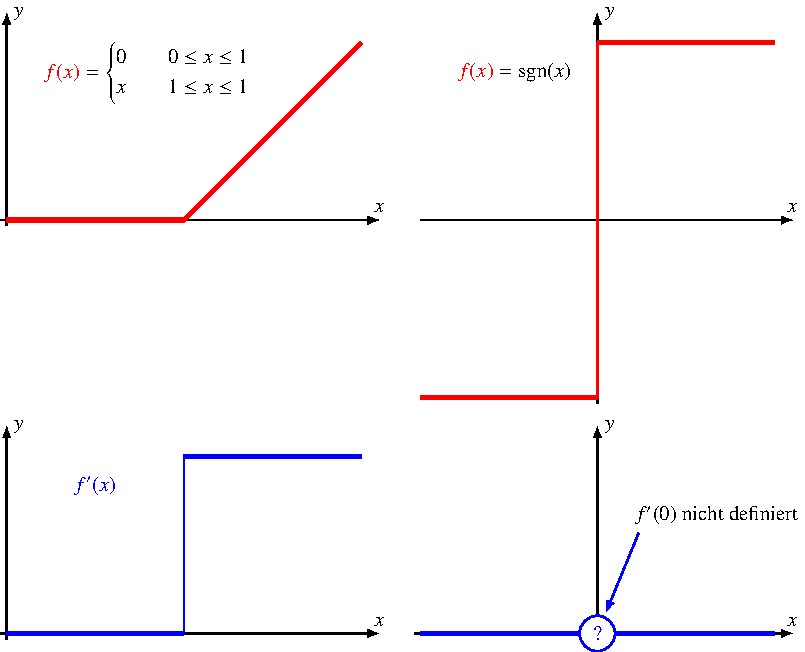
\includegraphics{chapters/010-skalarprodukt/images/schwach.pdf}
\caption{Schwache Ableitung einer nicht differenzierbaren Funktion.
Links die schwache Ableitung der Funktion von
Beispiel~\ref{buch:skalarprodukt:sobolevraum:bsp:schwachexistiert}.
Für die Signum-Funktion von
Beispiel~\ref{buch:skalarprodukt:sobolevraum:bsp:schwachexistiertnicht}
existiert die schwache Ableitung nicht, sie lässt für den Punkt $0$
nicht definieren.
\label{buch:skalarprodukt:sobolevraum:fig:schwach}}
\end{figure}
%
Die in Abbildung~\ref{buch:skalarprodukt:sobolevraum:fig:schwach} links
dargestellte Funktion
\[
f\colon (0,1) \to \mathbb{R}
:
x \mapsto
\begin{cases}
x&\qquad\text{für $0<x<1$}\\
1&\qquad\text{für $1\le x<2$}
\end{cases}
\]
ist stetig und integrierbar, aber sie ist an der Stelle $x=1$ nicht
differenzierbar.
Wir suchen die schwache Ableitung $v$ von $f$.

In einer Umgebung eines Punktes $x>1$ können wir Testfunktionen $\varphi$
so wählen, dass ihr Träger vollständig im Inneren des Intervals $(1,2)$
enthalten ist.
Mit diesen Testfunktionen können wir so rechnen, wie wenn $f$ die konstante
Funktion $1$ ist.
Das bedeutet für das Skalarprodukt
\[
\langle f,\varphi'\rangle
=
\int_1^2 \varphi'(x)\,dx
=
[\varphi(x)]_0^1 = 0.
\]
Das Skalarprodukt mit jeder beliebigen Testfunktion ist $0$, wir
müssen also $v(x)=0$ wählen.

Für $x$ im Teilinterval $(0,1)$ können wir die Testfunktionen so wählen,
dass der Träger vollständig im Inneren  von $(0,1)$ enthalten ist und
somit $f$ als die beliebig oft stetig differenzierbare Funktion $x$
behandelt werden darf.
Für das Skalarprodukt folgt dann
\[
-\langle f,\varphi'\rangle
=
-\int_0^1 f(x)\,\varphi'(x)\,dx
=
-\int_0^1 x\varphi'(x)\,dx
=
-[x\varphi(x)]_0^1 +\int_0^1 \varphi(x)\,dx
=
\langle 1,\varphi(x)\rangle,
\]
in diesem Teil des Intervals muss die schwache Ableitung den Wert $1$ 
haben.

Wir haben somit gefunden, dass die schwache Ableitung von $f$ die
Funktion
\[
v(x) = \begin{cases}
1&\qquad\text{für $0\le x<1$}
\\
0&\qquad\text{für $1< x<2$}
\end{cases}
\]
ist.
Wir kontrollieren dies, indem wir das Skalarprodukt für beliebige 
Testfunktionen $\varphi$ nachrechnen:
\begin{align*}
\langle v,\varphi\rangle
&=
\int_0^2 v(x)\,\varphi(x)\,dx
=
\int_0^1 1\,\varphi(x)\,dx
+
\int_1^2 0\,\varphi(x)\,dx.
\intertext{Jedes dieser Integrale kann man partiell integrieren:}
&=
[x\varphi(x)]_0^1 - \int_0^1 x\varphi'(x)\,dx
+
[1\varphi(x)]_1^2 - \int_1^2 1\varphi'(x)\,dx
\\
&=
\varphi(1) + \varphi(2) - \varphi(1) - \int_0^2 f(x)\,\varphi'(x)\,dx.
\intertext{Da $2$ ein Randpunkt ist, ist $\varphi(2)=0$, so dass sich}
&=-\langle f,\varphi'\rangle.
\end{align*}
ergibt.
Die Funktion $v$ ist also die schwache Ableitung von $f$.
\end{beispiel}

Eine Funktion in $W^{1,2}(\Omega)$ hat eine schwache Ableitung,
wie das Beispiel gezeigt hat, muss die Ableitung keine stetige
Funktion sein.
Ausserdem ist jede andere Funktion, die sich von der schwachen
Ableitung auf einer Menge vom Mass 0 unterscheidet, genauso eine
schwache Ableitung.
Trotzdem kann eine Funktion mit einer schwachen Ableitung nicht
beliebig ``wild'' sein, wie das folgende Beispiel zeigt.

\begin{beispiel}
\label{buch:skalarprodukt:sobolevraum:bsp:schwachexistiertnicht}
Die Signum-Funktion
\[
f\colon (-1,1) = \operatorname{sgn}(x) =
\begin{cases}
         - 1&\qquad\text{für $-1<x<0$}\\
\phantom{-}0&\qquad\text{für $x=0$}\\
\phantom{-}1&\qquad\text{für $0<x<1$}
\end{cases}
\]
ist nicht stetig (Abbildung~\ref{buch:skalarprodukt:sobolevraum:fig:schwach}).
$f$ ist fast überall konstant, in beiden Teilintervallen $(-1,0)$ und
$(0,1)$ ist die einzige mögliche schwache Ableitung von $f$ die
Nullfunktion.
Trotzdem kann $0$ nicht die schwache Ableitung von $f$ sein.
Wir wählen eine Testfunktion $\varphi$, die im Punkt $x=0$ von
Null verschieden ist.
Wäre $v$ eine schwache Ableitung von $f$, dann müsste
\begin{align*}
\langle v,\varphi\rangle
&=
-\langle f,\varphi'\rangle
=
-\int_{-1}^1 f(x) \varphi'(x)\,dx
\\
&=
-\int_{-1}^0 (-1)\cdot \varphi'(x)\,dx
-\int_{0}^1 1\cdot \varphi'(x)\,dx
=
\int_{-1}^0 \varphi'(x)\,dx
-
\int_{0}^1 \varphi'(x)\,dx
\\
&=
[\varphi(x)]_{-1}^0
-
[\varphi(x)]_{0}^1
=
\varphi(0)-\varphi(-1)
-
\varphi(1)+\varphi(0)
\\
&=
2\varphi(0)
\ne 0.
\end{align*}
Andererseits ist die Nullfunktion der einzige Kandidat für die
schwache Ableitun, für die das Skalarprodukt $\langle v,\varphi\rangle=0$
ist.
Dieser Widerspruch zeigt, dass die Funktion $f$ kein schwache
Ableitung hat.
\end{beispiel}

Die schwache Ableitung ermöglicht also mit gewissen Funktionen zu arbeiten,
die keine Ableitung im traditionellen Sinne haben.
Dank der Definition mit Hilfe eines Skalarproduktes in einem 
Hilbert-Raum darf man sich die Funktionen als Grenzwerte von
Cauchy-Folgen vorstellen.

%
% Physikalische Rechtfertigung
%
\subsection{Physikalische Rechtfertigung der schwachen Ableitung}
Die schwache Ableitung ersetzt die mit Hilfe eines Differenzenquotienten
definierte Änderungsrate durch eine Änderungsrate, die durch Vergleich
mit einer in der Umgebung eines Punktes konzentrierten Testfunktion
ermittelt wird.
Auf den ersten Blick mag das als Konzession an die Präzision der Ideen
der Analysis erscheinen, die Newton erfunden hat, um die Physik auf eine
neue Grundlage zu stellen.
Dabei wird aber vergessen, dass der Differenialquotient eine physikalisch
nicht erreichbare Idealisierung darstellt.
Keine Messung kann in einem Punkt im geometrischen Sinn erfolgen.
Die Bestimmung einer Position eines Massepunktes zum Beispiel erfolgt
durch Beobachtung des Lichtes, das vom Massepunkt reflektiert wird.
Doch der Massepunkt ist kein Punkt im geometrischen Sinn, er ist ausgedehnt
über ein endliches Gebiet.
Auch ist die Messung nicht instantan, es wird Licht gemessen, welches
über ein Zeitintervall vom Massepunkt reflektiert wird.
Das Messresultat entsteht also notwendigerweise als Mittelwert der
Beobachtung einer sehr grossen Zahl von Photonen, die von verschiedenen
Stellen reflektiert wurden.
Ein solcher Mittelwert ist genau das, was ein Skalarprodukt
$\langle f,\varphi\rangle$ mit einer Testfunktion ermittelt.

Die Feldgleichungen der Elektrodynamik wurden von Maxwell ausgehend
von Faradays Ideen als partielle Differentialgleichungen formuliert.
Sie verknüpfen die Werte des elektrischen Feldes $\vec{E}$ und des
magnetischen Feldes $\vec{B}$ mit der Ladungsdichte $\varrho$
und der Stromdichte $\vec{\jmath}$, die die Felder erzeugen.
Doch sowohl die Ladungsdichte wie auch die Stromdichte sind Idealisierungen.
Ladungen und Ströme sind nicht stetig über den Raum verteilt, sondern 
in Elektronen oder Atomkernen konzentriert.
Die Ladungsdichte entsteht daraus durch Messung der Ladung in einem kleine
Raumgebiet und Mittelung, was man wieder als Skalarprodukt mit einer
Testfunktion beschreiben kann.

Das elektrische Feld wird gemessen, indem die Kraft auf eine Testladung
im Feld ermittelt wird.
Ausser den prinzipiellen Einschränkungen an die Genauigkeit der
Positionsmessung wissen wir auch aus der Quantenmechanik, dass so etwas
wie die exakte Position eines Teilchens nicht gibt, wir können nur eine
Wahrscheinlichkeitsverteilung dafür bekommen.
Die Kraft äussert sich in einer Geschwindigkeitsänderung, die aber erst
messbar wird, wenn man die Beschleunigung eine gewisse Zeit lang aufrecht
erhält.
Das Messresultat ist also wieder ein Mittelwert über viele Positionen
und Zeitpunkte, oder anders ausgedrückt ein Skalarprodukt mit einer
Testfunktion.

Weitere Beispiele kann man auch in der Fluiddynamik finden.
Die Navier-Stokes-Gleichungen beschreiben die Strömung eines Mediums
unter der Annahme, dass es durch die Dichte $\varrho$ und die
Geschwindigkeit exakt beschreiben lässt.
Das Medium setzt sich aber aus einzelnen Atomen zusammen, die Dichte
ist also bereits ein Mittelwertbildung.
Bei der Geschwindigkeit wird das Problem noch deutlicher.
Auch die Strömungsgeschwindigkeit eines Gases ist der Mittelwert der
Strömungsgeschwindigkeit der Teilchen. 
Die Geschwindigkeit einzelner Teilchen ist dabei meistens sehr viel
grösser, nämlich im Bereich der Schallgeschwindigkeit, und äussert sich
in der Temperatur des Gases, also der mittleren kinetischen Energie.
Es ist nicht sinnvoll, von der Temperatur eines einzelnen Atoms zu
sprechen.

Alle diese Beispiele zeigen, dass die Ableitung als Änderungsrate, die
mit einem Differenzenquotienten bestimmt werden kann, eine Idealisierung
ist.
Wir können dies sogar etwas formeller zeigen.
Sei $x(t)$ die Koordinate eines Massepunktes zur Zeit $t$.
Die Messung kann nicht instantan erfolgen, im besten Fall ist die
gemessene Position ein Integral der Form
\[
\hat{x}(t)
=
\int_{-\infty}^\infty x(\tau) \varphi(\tau - t)\,d\tau.
\]
Darin ist $\varphi$ eine Testfunktion mit Träger in der Nähe von $0$.
Schreiben wir $T_t\varphi(\tau) = \varphi(\tau -t)$, dann können wir
das Messresultat auch als Skalarprodukt
$\hat{x}(t)=\langle x,T_t\varphi\rangle$
schreiben.
Die Messung mit der gleichen Aparatur einen Moment $\Delta t$ später ergibt
\[
\hat{x}(t+\Delta t)
=
\int_{-\infty}^\infty x(\tau) \varphi(\tau-t-\Delta t)\,dt
=
\langle x, T_{t+\Delta t}\varphi\rangle.
\]
Die Geschwindigkeit als Differenzenquotient ist
\begin{equation}
\frac{
\hat{x}(t+\Delta t)-\hat{x}(t)
}{\Delta t}
=
\frac{
\langle f,T_{t+\Delta t}\varphi\rangle
-
\langle f,T_{t}\varphi\rangle
}{
\Delta t
}
=
\left\langle
f,\frac{T_{t+\Delta t}\varphi - \varphi}{\Delta t}
\right\rangle
\label{buch:skalarprodukt:sobolevlraum:eqn:geschwindigkeit}
\end{equation}
Die Funktion $(T_{t+\Delta t}\varphi-T_t\varphi)/\Delta t$ ist eine 
beliebig oft stetig differenzierbare Funktion, die im Grenzwert
$\Delta t\to 0$ gegen
\[
\frac{
\varphi(\tau - t - \Delta t)
-
\varphi(\tau - t)
}{
\Delta t
}
=
-
\frac{
\varphi(\tau - t + \delta) - \varphi(\tau - t)
}{
\delta
}
\to 
-
\varphi'(\tau - t)
\quad
\text{für $\delta = - \Delta \to 0$}
\]
konvergiert.
Der Differenzenquotient
\eqref{buch:skalarprodukt:sobolevlraum:eqn:geschwindigkeit}
konvergiert daher gegen
\[
\lim_{\Delta t\to 0}
\frac{
\hat{x}(t+\Delta t)-\hat{x}(t)
}{\Delta t}
=
\left\langle
x,
\lim_{\Delta t\to 0}
\frac{T_{t+\Delta t}\varphi-T_t\varphi}{\Delta t}
\right\rangle
=
\langle f,-\varphi'\rangle
=
-
\langle f, \varphi'\rangle.
\]
Dieses einfache Modell einer ``unscharfen'' Messung führt also automatisch
auf das Konzept der schwachen Ableitung.








%\uebungsabschnitt
%\aufgabetoplevel{chapters/010-potenzen/uebungsaufgaben}
%\begin{uebungsaufgaben}
%\uebungsaufgabe{101}
%\uebungsaufgabe{102}
%\uebungsaufgabe{103}
%\uebungsaufgabe{104}
%\end{uebungsaufgaben}
%\endgroup


%
% chapter.tex -- Skalarprodukt
%
% (c) 2021 Prof Dr Andreas Müller, Hochschule Rapperswil
%
% !TeX spellcheck = de_CH
\chapter{Skalarprodukte
\label{buch:chapter:skalarprodukte}}
\kopflinks{Skalarprodukte}

%
% 1-definition.tex
%
% (c) 2023 Prof Dr Andreas Müller, OST Ostschweizer Fachhochschule
%
\section{Definition
\label{buch:opertoren:section:definition}}
\kopfrechts{Definition}


%
% 2-cauchyschwarz.tex
%
% (c) 2022 Prof Dr Andreas Müller, OST Ostschweizer Fachhochschule
%
\section{Ungleichungen
\label{buch:skalarprodukte:section:cauchyschwarz}}
\kopfrechts{Cauchy-Schwarz-Ungleichung}
In der Vektorgeometrie wird gelehrt, dass die Länge eines Vektors $u$
durch die Norm $\|u\|$ wiedergegeben wird und dass die geometrische
Intuition dazu passt.
Dazu gehört vor allem, dass die Dreiecksungleichung erfüllt ist,
dass also für drei Punkt $A$, $B$ und $C$
\begin{equation}
\overline{AB} \le \overline{AC} + \overline{BC}
\label{skalarprodukt:ungleichungen:eqn:dreieck}
\end{equation}
gilt.
In Vektorform bedeutet dies, dass
\[
\| b-a\|
\le
\| c-a\| + \|b-c\|.
\]
Schreibt man $u=c-a$ und $v=b-c$, dann ist $u+v=b-a$ und somit
\begin{equation}
\| u+v\| \le \|u\| + \|v\|.
\label{skalarprodukt:cauchyschwarz:eqn:dreieck0}
\end{equation}
Dies ist die Dreiecksungleichung in
Vektorform~\eqref{skalarprodukt:cauchyschwarz:eqn:dreieck0}.
Ziel dieses Abschnitts ist zu zeigen, dass jedes reelle oder
komplexe Skalarprodukt diese und weitere Eigenschaften automatisch
mitbringt.

%
% Cauchy-Schwarz-Ungleichung
%
\subsection{Cauchy-Schwarz-Ungleichung}
Sei also $\langle\;\,,\;\rangle$ ein reelles oder komplexes Skalarprodukt
auf dem Vektorraum $V$,
insbesondere ist $\langle v,v\rangle\ge 0$ für beliebige Vektoren $v\in V$.
Für zwei Vektoren $x,y\in V$ und $t\in \mathbb{R}$  gilt daher
\begin{align}
0
&\le
\| x+ty\|^2
=
\langle x+ty,x+ty\rangle
=
\langle x,x\rangle
+
t\langle x,y\rangle
+
t\langle y,x\rangle
+
t^2
\langle y,y\rangle.
\label{skalarprodukt:cauchyschwarz:eqn:quadrat}
\end{align}
Für ein reelles Skalarprodukt ist $\langle x,y\rangle=\langle y,x\rangle$
und damit
\begin{align}
0
&\le
\|x\|^2 + 2t\langle x,y\rangle + t^2 \|y\|^2.
\label{buch:skalarprodukt:cauchyschwarz:eqn:cspoly}
\end{align}
Dies ist ein quadratisches Polynom in der Variablen $t$, dessen Minimum
nicht negativ sein darf.

%
% Minimum eines quadratischen Polynoms
%
\subsubsection{Minimum eines quadratischen Polyoms}
Ein beliebiges quadratisches Polynom
\[
p(t)=at^2+bt+c
\]
kann durch
quadratisches Ergänzen in die Form
\[
p(t)
=
a\biggl(t+\frac{b}{2a}\biggr)^2 -\frac{b^2}{4a}+c
\]
gebracht werden.
Daraus kann man ablesen, dass das Minimum an der Stelle
\[
t_0
=
-\frac{b}{2a}
\]
angenommen wird und den Wert 
\begin{equation}
p(t_0)
=
c-\frac{b^2}{4a}
\end{equation}
hat.
Die gleiche Lösung kann natürlich auch durch Bestimmung des Minimums
von $p(t)$ mit Hilfe der Bedingung $p'(t_0)=0$ gefunden werden.

%
% Cauchy-Schwarz-Ungleichung für einen reellen Vektorraum
%
\subsubsection{Cauchy-Schwarz-Ungleichung für einen reellen Vektorraum}
Für~\eqref{buch:skalarprodukt:cauchyschwarz:eqn:cspoly}
ist
\[
a=\|y\|^2,\quad
b=2\langle x,y\rangle
\quad\text{und}\quad
c=\|x\|^2.
\]
Daher folgt aus~\eqref{buch:skalarprodukt:cauchyschwarz:eqn:cspoly}
\[
0
\le
\|x\|^2 - \frac{\langle x,y\rangle^2}{\|y\|^2}
\qquad\Rightarrow\qquad
\langle x,y\rangle^2 \le \|x\|^2\, \|y\|^2
\qquad\Rightarrow\qquad
|\langle x,y\rangle| \le \|x\|\, \|y\|.
\]
Dies ist die Cauchy-Schwarz-Ungleichung für das Skalarprodukt
$\langle \;\,,\;\rangle$.

\begin{satz}[Cauchy-Schwarz]
\label{buch:skalarprodukt:cauchy-schwarz:satz:reell}
Ein reelles Skalarprodukt $\langle\;\,,\;\rangle$ auf dem reellen Vektorraum
$V$ erfüllt die Cauchy-Schwarz-Ungleichung
\[
|\langle x, y\rangle| \le \|x\|\,\|y\|
\]
für $x,y\in V$.
\end{satz}

%
% Cauchy-Schwarz-Ungleichung für einen komplexen Vektorraum
%
\subsubsection{Cauchy-Schwarz-Ungleichung für einen komplexen Vektorraum}
Für ein komplexes Skalarprodukt ist das Produkt $\langle x,y\rangle$
nicht mehr unbedingt reell und kann damit nicht mehr direkt mit den
Normen $\|x\|^2u$ und $\|y\|^2$ vergleichen.
Wir ersetzen daher $t$ durch
$t\langle y,x\rangle=t\overline{\langle x,y\rangle}$
und erhalten 
\begin{align*}
0
\le
\|x+t\langle y,x\rangle y\|^2
&=
\langle x,x\rangle
+t\langle y,x\rangle \langle x,y\rangle
+t\overline{\langle y,x\rangle}\langle y,x\rangle
+t^2\langle y,y\rangle
\\
&=
\|x\|^2
+
t
2|\langle x,y\rangle|^2
+
t^2 |\langle x,y\rangle|^2
\|y\|^2.
\end{align*}
Dies ist wieder ein quadratisches Polynom, diesmal mit den Koeffizienten
\[
a= |\langle x,y\rangle|^2 \|y\|^2,
\quad
b= 2|\langle x,y\rangle|^2
\quad\text{und}\quad
c= \|x\|^2.
\]
Das Minimum dieses Polynoms ist nach
\[
0
\le
c-\frac{b^2}{4a}
=
\|x\|^2 - \frac{|\langle x,y\rangle|^4}{|\langle x,y\rangle|^2\,\|y\|^2}
=
\|x\|^2 - \frac{|\langle x,y\rangle|^2}{\|y\|^2}
\quad\Rightarrow\quad
|\langle x,y\rangle|^2 \le \|x\|^2\,\|y\|^2
\quad\Rightarrow\quad
|\langle x,y\rangle \le \|x\|\,\|y\|.
\]
Dies ist die Cauchy-Schwarz-Ungleichung für einen komplexen Vektorraum.

\begin{satz}[Cauchy-Satz]
\label{buch:skalarprodukt:cauchy-schwarz:satz:komplex}
Ein komplexes Skalarprodukt $\langle\;\,,\;\rangle$ auf dem komplexen Vektorraum
$V$ erfüllt die Cauchy-Schwarz-Ungleichung
\[
|\langle x, y\rangle| \le \|x\|\,\|y\|
\]
für $x,y\in V$.
\end{satz}

Man beachte, dass die
Sätze~\ref{buch:skalarprodukt:cauchy-schwarz:satz:reell}
und
\ref{buch:skalarprodukt:cauchy-schwarz:satz:komplex}
nur die Axiome eines Skalarproduktes verwenden.
Sie gelten also
ganz unabhängig von der konkreten Definition des Skalarproduktes,
solange die Eigenschaften eines Skalarproduktes gegeben sind.

\begin{beispiel}
Die sesquilineare Funktion
\[
\langle x,y\rangle
=
\sum_{i=1}^n\overline{x}_i y_i
\]
für Vektoren $x,y\in\mathbb{C}^n$ ist positiv definit, denn
\[
\langle x,x\rangle
=
\sum_{i=1}^n \overline{x}_i x_i = \sum_{i=1}^n |x_i|^2 > 0
\]
für $x\ne 0$.
Nach Satz~\ref{buch:skalarprodukt:cauchy-schwarz:satz:komplex}
gilt daher
\[
\biggl|
\sum_{i=1}^n \overline{x}_i y_i
\biggr|
\le
\sqrt{\sum_{i=1}^n |x_i|^2} \sqrt{\sum_{i=1}^n |y_i|^2}
\quad\text{oder auch}\quad
\biggl|
\sum_{i=1}^n x_i y_i
\biggr|
\le
\sqrt{\sum_{i=1}^n |x_i|^2} \sqrt{\sum_{i=1}^n |y_i|^2}
\]
für beliebige Vektoren $x,y\in\mathbb{C}^n$.
\end{beispiel}

\begin{beispiel}
Die sesquilineare Funktion
\[
\langle f,g\rangle
=
\int_a^b \overline{f(x)} g(x)\,dx
\]
für komplexwertige, stetige Funktion auf dem Intervall $[a,b]$
ist positiv definit, denn
\[
\langle f,f\rangle
=
\int_a^b \overline{f(x)} f(x)\,dx
=
\int_a^b |f(x)|^2\,dx
\ge 0
\]
für $f\ne 0$.
Nach Satz~\ref{buch:skalarprodukt:cauchy-schwarz:satz:komplex}
gilt daher
\begin{align*}
\biggl|\int_a^b \overline{f(x)}g(x)\,dx\biggr|
&\le
\sqrt{\int_a^b |f(x)|^2\,dx}
\sqrt{\int_a^b |g(x)|^2\,dx}
\intertext{oder auch}
\biggl|\int_a^b f(x) g(x)\,dx\biggr|
&\le
\sqrt{\int_a^b |f(x)|^2\,dx}
\sqrt{\int_a^b |g(x)|^2\,dx}
\end{align*}
für beliebige komplexwertige stetige Funktionen $f,g$ auf dem
Intervall $[a,b]$.
\end{beispiel}

%
% Dreiecksungleichung
%
\subsection{Dreiecksungleichung}
Die Intuition einer Längenmessung basiert auf der
Dreiecksungleichung~\eqref{skalarprodukt:ungleichungen:eqn:dreieck}.
Sie ist gleichbedeutend mit der
Vektorform~\eqref{skalarprodukt:cauchyschwarz:eqn:dreieck0}
der Ungleichung.

Die Cauchy-Schwarz-Ungleichung ermöglicht nun, diese Ungleichung
nachzurechnen.
Die Norm von $\|x+y\|^2$ ist
\[
\|x+y\|^2
=
\langle x+y,x+y\rangle
=
\langle x,x\rangle
+
\langle x,y\rangle
+
\langle y,x\rangle
+
\langle y,y\rangle
=
\|x\|^2 + 2\operatorname{Re}\langle x,y\rangle + \|y\|^2.
\]
Den mittleren Term kann man mit der Cauchy-Schwarz-Ungleichung
umformen:
\begin{align*}
\|x\|^2 + 2\operatorname{Re}\langle x,y\rangle + \|y\|^2.
&\le
\|x\|^2 + 2|\operatorname{Re}\langle x,y\rangle| + \|y\|^2.
\\
&\le
\|x\|^2 + 2|\langle x,y\rangle| + \|y\|^2.
\\
&\le
\|x\|^2 + 2\|x\|\,\|y\| + \|y\|^2
=
(\|x\| + \|y\|)^2.
\end{align*}
Durch Ziehen der Wurzel folgt
\[
\|x+y\| \le \|x\| + \|y\|.
\]
Damit ist der folgende Satz bewiesen.

\begin{satz}[Dreiecksungleichung]
Für die Norm zu einem beliebigen Skalarprodukt auf dem reellen
oder komplexen Vektorraum $V$ gilt die Dreiecksungleichung
\[
\|x+y\| \le \|x\| + \|y\|
\]
für $x,y\in V$.
\end{satz}

%
% Normen
%
\subsection{Normen
\label{skalarprodukt:cauchyschwarz:subsection:norm}}
Das Skalarprodukt ist nicht die einzige Möglichkeit, eine Norm auf
einem Vektorraum zu definieren.
Zum Beispiel kann man auf $\mathbb{C}^n$ die sogenannte $l^1$-Norm
definieren.

\begin{definition}
Die Funktion
\[
\|x\|_1
=
\sum_{i=1}^n |x_i|
\]
für $x\in\mathbb{C}^n$ heisst die {\em $l^1$-Norm} auf $\mathbb{C}^n$.
\end{definition}

Die Funktion $\|\cdot\|_1$ ist eine Norm im Sinne der folgenden Definition.

\begin{definition}
Eine Funktion $\|\cdot\| \colon V\to\mathbb{R}$ auf einem reellen
oder komplexen Vektorraum $V$ heisst eine {\em Norm}, wenn Sie die
folgenden Bedingungen erfüllt
\begin{enumerate}
\item
$\|\lambda x\| = |\lambda|\, \|x\|$ für $x\in V$ und $\lambda\in \Bbbk$
\item
Für alle Vektoren $x\in V$ mit $x\ne 0$ gilt $\|x\|>0$.
\item
Dreiecksungleichung: $\|x+y\| \le \|x\| + \|y\|$ für alle $x,y\in V$
\end{enumerate}
\end{definition}

Es ist klar, dass die $l^1$-Norm die Bedingungen~1 und 2 erfüllt.
Aber auch die Bedingung~3 kann man leicht  nachprüfen:
\[
\|x+y\|_1
=
\sum_{i=1}^n |(x+y)_i|
=
\sum_{i=1}^n |x_i+y_i|
\le
\sum_{i=1}^n(|x_i|+|y_i|)
=
\sum_{i=1}^n|x_i|
+
\sum_{i=1}^n|y_i|
=
\|x\|_1 + \|y\|_1,
\]
wozu wir nur die Dreiecksungleichung $|a+b|\le |a| + |b|$ für reelle 
oder komplexe Zahlen $a,b$ benötigen.

\begin{beispiel}
Die Funktion
\[
\|x\|_\infty = \sup_{1\le i\le n} |x_i|
\]
ist eine Norm auf $\mathbb{C}^n$.
\end{beispiel}

Auch in diesem Fall sind die Bedingungen~1 und 2 ganz offensichtlich erfüllt.
Für die Dreiecksungleichung rechnen
\begin{align*}
\|x+y\|_\infty
&=
\sup_{1\le i\le n} |x_i+y_i|
\le
\sup_{1\le i\le n} (|x_i|+|y_i|)
\le
\sup_{1\le i\le n} |x_i|+\sup_{1\le i\le n}|y_i|
=
\|x\|_\infty + \|y\|_\infty.
\end{align*}
Somit ist $\|\cdot\|_\infty$ eine Norm auf $\mathbb{C}^n$.

%
% Polaridentität
%
\subsection{Polaridentität}
Die durch das Skalarprodukt definierte Norm
\( \|x\|^2=\langle x,x\rangle \)
ist nach Abschnitt~\ref{skalarprodukt:cauchyschwarz:subsection:norm}
ein Spezialfall einer Norm.
Ist es möglich, für eine Norm, die von einem Skalarprodukt herkommt,
das Skalarprodukt wieder zu rekonstruieren?

%
% Reelles Skalarprodukt aus der Norm
%
\subsubsection{Reelles Skalarprodukt aus der Norm}
Die Antwort gibt der folgende Satz.

\begin{satz}[Polaridentität]
\label{skalarprodukt:cauchyschwarz:satz:polarformel}
Ist $\|\cdot\|$ die Norm zu einem Skalarprodukt auf dem reellen Vektorraum
$V$, dann kann das Skalarprodukt zweier Vektoren $x,y\in V$ mittels
der sogenannten {\em Polaridentität}
\index{Polaridentität}%
\begin{equation}
\langle x, y\rangle
=
\frac12\bigl(
\|x+y\|^2 - \|x\|^2 - \|y\|^2 
\bigr)
\label{skalarprodukt:cauchyschwarz:eqn:polar}
\end{equation}
berechnet werden.
\end{satz}

\begin{proof}[Beweis]
Die Gleichung
\begin{align*}
\|x+y\|^2
&=
\langle x+y,x+y\rangle
=
\|x\|^2 + 2\langle x,y\rangle + \|y\|^2 
\end{align*}
kann nach $\langle x,y\rangle$ aufgelöst werden und ergibt
die behauptete Formel~\eqref{skalarprodukt:cauchyschwarz:eqn:polar}.
\end{proof}

% 
% Parallelogrammgleichung
%
\subsubsection{Parallelogrammgleichung}
\begin{figure}
\centering
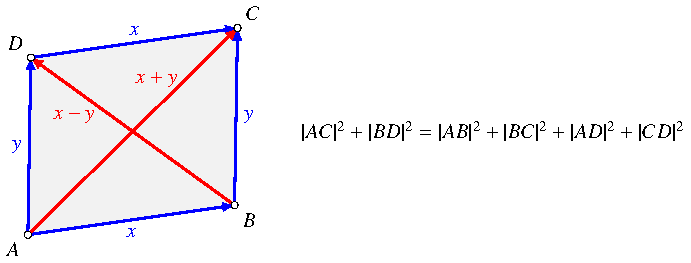
\includegraphics{chapters/010-skalarprodukt/images/parallelogramm.pdf}
\caption{Parallelogrammregel für eine Norm, die aus einem Skalarprodukt
entsteht.
\label{skalarprodukt:cauchyschwarz:fig:parallelogramm}}
\end{figure}
Die Polaridentitäten können auch noch in einer anderen Form geschrieben
werden.
Dazu berechnet man zusätzlich die Norm von $x-y$:
\begin{align*}
\|x+y\|^2
&=
\|x\|^2 + \|y\|^2 + 2\langle x, y\rangle
\\
\|x-y\|^2
&=
\|x\|^2 + \|y\|^2 - 2\langle x, y\rangle
\\
\|x+y\|^2 +\|x-y\|^2
&=
2\|x\|^2 + 2\|y\|^2
\end{align*}

\begin{satz}
\label{skalarprodukt:cauchyschwarz:satz:parallelgramm}
Für eine Norm, die von einem reellen Skalarprodukt herkommt, gilt die
Parallelogrammformel
\begin{equation}
\|x+y\|^2 +\|x-y\|^2
=
2\|x\|^2 + 2\|y\|^2.
\label{skalarprodukt:cauchyschwarz:eqn:parallelgramm}
\end{equation}
(Abbildung~\ref{skalarprodukt:cauchyschwarz:fig:parallelogramm})
\end{satz}

Das Skalarprodukt kann man damit auf verschiedene Weise aus der
Norm gewinnen:
\begin{equation}
\begin{aligned}
\langle x, y\rangle
&=
{\textstyle\frac12}\bigl( \|x\|^2 + \|y\|^2 - \|x+y\|^2 \bigr)
\\
&=
{\textstyle\frac12}\bigl(
\|x+y\|^2
-
\|x\|^2 
-
\|y\|^2
\bigr)
\\
&=
{\textstyle\frac14}\bigl(
\|x+y\|^2 - \|x-y\|^2
\bigr).
\end{aligned}
\label{skalarprodukt:cauchyschwarz:eqn:realteil}
\end{equation}
Nur die letzte Formel ist noch nicht gut begründet.
Man kann aber sofort nachrechnen, dass 
\begin{align*}
\|x+y\|^2&=\|x\|^2+2\langle x,y\rangle+\|y\|^2\\
\|x-y\|^2&=\|x\|^2-2\langle x,y\rangle+\|y\|^2
\intertext{die Differenz}
\|x+y\|^2 - \|x-y\|^2 &= 4\langle x,y\rangle
\qquad
\Rightarrow
\qquad
\langle x,y\rangle
=
\frac14\bigl(\|x+y\|^2 - \|x-y\|^2\bigr)
\end{align*}
haben.

%
% Komplexes Parallelogramm aus der Norm
%
\subsubsection{Komplexe Skalarprodukt}
Das Resultat von Satz~\ref{skalarprodukt:cauchyschwarz:satz:polarformel}
gilt in abgeänderter Form auch für komplexe Skalarprodukte.
Da das Skalarprodukt auch einen nichtverschwindenen Imaginärteil haben
kann, wird eine zusätzliche Gleichung zur Berechnung des Imaginärteils
nötig.
Eine solche kann gewonnen werden, indem zusätzlich die Normen
$\|x+iy\|^2$ und $\|x-iy\|^2$ berechnet werden.
Dazu ist zu beachten, dass
\[
\langle x,y\rangle
-
\langle y,x\rangle
=
\langle x,y\rangle
-
\overline{
\langle x,y\rangle
}
=
2i\operatorname{Im}\langle x,y\rangle
\]
Damit erhält man
\begin{align*}
\|x+iy\|^2 &= \|x\|^2 + i\langle x,y\rangle - i\langle y,x\rangle + \|y\|^2 
           = \|x\|^2 + 2\operatorname{Im}\langle x,y\rangle + \|y\|^2 \\
\|x-iy\|^2 &= \|x\|^2 - i\langle x,y\rangle + i\langle y,x\rangle + \|y\|^2 
           = \|x\|^2 - 2\operatorname{Im}\langle x,y\rangle + \|y\|^2.
\end{align*}
Damit kann man nach dem Imaginärteil des Skalarproduktes auflösen und
die Formeln
finden, die den Formeln
\eqref{skalarprodukt:cauchyschwarz:eqn:realteil}
für das reelle Skalarprodukt entsprechen.
\eqref{skalarprodukt:cauchyschwarz:eqn:realteil}
Formeln bleiben gültig als Formeln für den Realteil des Skalarproduktes.
Damit haben wir den folgenden Satz gefunden.

\begin{satz}[Polaridentitäten für ein komplexes Skalarprodukt]
Ist $\|\cdot\|$ die Norm, die aus dem komplexen Skalarprodukt
$\langle\;\,,\;\rangle$ auf einem Vektorraum $V$ gewonnen wurde,
dann können Real- und Imaginärteil mit den Formeln
\begin{align*}
\operatorname{Re}\langle x,y\rangle
&=
{\textstyle\frac12}\bigl(
\|x+y\|^2 - \|x\|^2 -\|y\|^2
\bigr)
\\
&=
{\textstyle\frac12}\bigl(
\|x\|^2 +\|y\|^2 - \|x+y\|^2
\bigr)
\\
&=
{\textstyle\frac14}\bigl(
\|x+y\|^2 - \|x-y\|^2
\bigr),
\\
\operatorname{Im}\langle x,y\rangle
&=
{\textstyle\frac12}\bigl(
\|x+iy\|^2-\|x\|^2-\|y\|^2
\bigr)
\\
&=
{\textstyle\frac12}\bigl(
\|x\|^2+\|y\|^2-\|x-iy\|^2
\bigr)
\\
&=
{\textstyle\frac14}\bigl(
\|x+iy\|^2
-
\|x-iy\|^2
\bigr)
\end{align*}
für beliebige Vektoren $x,y\in V$
allein aus Werten der Norm berechnet werden.
\end{satz}


%
% 3-funktionenraeume.tex
%
% (c) 2022 Prof Dr Andreas Müller, OST Ostschweizer Fachhochschule
%
\section{Funktionenräume
\label{buch:skalarprodukt:section:funktionenraeume}}
\kopfrechts{Funktionenräume}
Ziel der harmonischen Analysis ist die effiziente Approximation einer
grossen Klasse von Funktionen.
Als approximierende Funktionen kommen stetige Funktionen, Polynome,
trigonometrische Polynome oder eine ähnlich, einfach konstruierbare
Funktionenfamilie in Frage.
Es gilt zunächst herauszufinden, was ``Approximation'' genau heissen
soll und von welchen Funktionen man überhaupt erwarten kann, dass sie
approximiert werden können.

%
% Stetige Funktionen
%
\subsection{Stetige Funktionen
\label{buch:skalarprodukt:subsection:stetige-funktionen}}
Der frühe intuitive Funktionsbegriff ging oft von der Vorstellung einer
in einem Strich gezeichneten Kurve aus, wie man sie von den Graphen
der Polynome oder der trigonometrischen Funktionen her kennt.
In moderner Sprechweise sind dies die stetigen Funktionen.

\begin{definition}
Eine Funktion $f\colon I\to\mathbb{R}$ mit $I\subset \mathbb{R}$
heisst stetig in einem Punkt $x_0\in I$, wenn für jedes $\varepsilon>0$
ein $\delta>0$ existiert derart, dass $f(x)-f(x_0)|<\delta$ sobald
$|x-x_0|<\varepsilon$.
\end{definition}

Nur die Eigenschaft, eine Abstandsmessung zu besitzen, wird vom
Definitionsbereich $I\subset \mathbb{R}$ verlangt.
Der Stetigkeitsbegriff kann daher verallgemeinert werden auf den
Begriff des metrischen Raumes.

\begin{definition}
Eine {\em Metrik} auf einer Menge $X$ ist eine Funktion
\index{Metrik}%
$d\colon X\times X\to \mathbb{R}$
mit den folgenden Eigenschaften
\begin{enumerate}
\item
Positiv definit: $d(x,y)\ge 0$ und $d(x,y)$ genau dann, wenn $x=y$.
\item
Symmetrie: \(d(x,y)=d(y,x)\)
\item
Dreiecksungleichung: \( d(x,y) \le d(x,z) + d(z,y) \).
\end{enumerate}
Ein {\em metrischer Raum} ist ein Menge $X$ mit einer Metrik.
\index{matrischer Raum}%
\end{definition}

In einem metrischen Raum ist der Begriff des Grenzwertes übertragbar.
Mit dem Begriff des Grenzwertes lässt sich auch der Begriff der
Stetigkeit verallgemeinern.

\begin{definition}
Ist $x_n\in X$ eine Folge von Punkten in einem metrischen Raum $X$,
dann heisst $x$ der Grenzwert der Folge $x_n$, wenn es für jedes
$\varepsilon>0$ ein $N>0$ gibt derhart, dass
$d(x_n,x)\le \varepsilon$ für alle $n>N$.
Eine Funktion $f\colon X\to Y$ zwischen metrischen Räumen heisst
stetig im Punkt $x\in X$, wenn für jede Folge $x_n\in X$ mit
Grenzwert $x$ auch die Folge $y_n=f(x_n)\in Y$ konvergiert und
den Grenzwert $y=f(x)$ hat.
\end{definition}

Teilmengen von $\mathbb{R}$ oder $\mathbb{R}^n$ tragen natürlich
die Struktur eines metrischen Raumes mit der Abstandsmessung in 
$\mathbb{R}^n$ als Metrik
\[
d(x,y) = \sqrt{(x_1-y_1)^2 + \ldots + (x_n-y_n)^2} = \|x-y\|.
\]
Die Eigenschaften einer Metrik wurden bereits in Abschnitt
\ref{buch:skalarprodukte:section:cauchyschwarz} nachgewiesen.

Der Begriff des Grenzwertes klärt, was mit der Approximation von $x$
durch eine Folge $x_n$ gemeint ist.
Wenn man darauf aufbauend die Konvergenz einer Folge von Funktionen
gegen eine Grenzfunktion definieren will, braucht man einen Abstansbegriff
zwischen Funktionen.
Ein erster Versuch könnte sein, als Abstand zwischen zwei Funktionen
$f$ und $g$ die Funktion
\[
d(f,g) = |f(x_0) - g(x_0)|.
\]
Die Menge der Funktionen wird dadurch jedoch nicht zu einem metrischen
Raum.
Zwar gilt sicher die Symmetrie und Dreiecksungleichung, und auch 
$d(f,g)\ge 0$ für beliebige Funktionen.
Aber wenn $d(f,g)=0$ ist, heisst das nur, dass $f$ und $g$ im Punkt
$x_0$ den gleichen Wert haben.
Ausser in trivialen Fällen wird es Funktionen geben, die zwar im Punkt
$x_0$ übereinstimmen, sich aber in mindestens einem anderen Punkt
unterscheiden.

%
% Normierte Räume
%
\subsubsection{Normierte Räume}
Die stetigen Funktionen bilden aber keine strukturlose Menge, sie
bilden einen Vektorraum: die Summe von stetigen Funktionen ist ebenfalls
stetig, multiplizieren einer stetigen Funktion mit einem Skalar führt
nicht aus der Menge der stetigen Funktionen heraus.
Die für den Grenzwertbegriff von Funktionen verwendete Abstandsmessung 
sollte der Vektorraumstruktur ebenfalls Rechnung tragen.

\begin{definition}
\label{buch:skalaprodukt:funktionenraume:def:norm}
Sei $V$ ein Vektorraum über $\mathbb{R}$, dann heisst eine Funktion
\( \|\;\cdot\;\| \colon V \to \mathbb{R}\) eine {\em Norm}, wenn gilt
\index{Norm}
\begin{enumerate}
\item
Definit: $ \|x\| = 0 \Rightarrow x=0$
\item
Homogeneität: $ \| \lambda x \| = |\lambda| \cdot \|x\|$
\item
Dreiecksungleichung: $\|x+y\| \le \|x\| + \|y\|$
\end{enumerate}
Ein {\em normierter Raum} ist ein Vektorraum $V$ mit einer Norm.
\end{definition}

%
% Vollständigkeit
%
\subsubsection{Vollständigkeit}
In den rationalen Zahlen hat nicht jede Folge einen Grenzwert.
Die Zahl $\sqrt{2}$ lässt sich beliebig genau durch rationale Zahlen
approximieren, sie ist aber nicht in $\mathbb{Q}$.
Ähnlich lässt sich die Funktion $x\mapsto \sqrt{x}$ beliebig genau 
durch Polyome approximieren, sie ist aber selbst kein Poylnome

\begin{definition}
Ein Folge $x_n\in X$ in einem metrischen Raum heisst {\em Cauchy-Folge},
wenn es für jedes $\varepsilon>0$ ein $N>0$ gibt derart, dass 
$|x_n-x_m|<\varepsilon$ wenn $n,m>N$ ist.
\end{definition}

Cauchy-Folgen sind also Folgen, die sich für genügend grossen Index
kaum mehr ändern und für die man daher Konvergenz erwarten würde.

\begin{definition}
Ein normierter Raum heisst {\em vollständig} oder ein Banach-Raum,
wenn jede Cauchy-Folge einen Grenzwert hat.
\end{definition}

Die rationalen Zahlen $\mathbb{Q}$ bilden keinen vollständigen
metrischen Raum, aber die reellen Zahlen $\mathbb{R}$ enthalten
alle Grenzwerte von Cauchy-Folgen, $\mathbb{R}$ ist eine vollständiger
metrischer Raum.
Die Menge der Polynome, betrachtet als Teilmenge der Menge der
stetigen Funktionen $[0,1]\to\mathbb{R}$ ist nicht vollständig,
da es eine Folge $f_n(x)$ von Approximationsfunktionen der Funktion
$x\mapsto \sqrt{x}$ gibt.
Als Cauchy-Folge konvergiert sie zwar gegen eine stetige Funktion,
aber die Grenzfunktion ist nicht mehr im Raum der Polynome.

Das Ziel der folgenden Kapitel ist also, zu geeignet interessanten
Funktionenfamilien ``gute'' Normen zu finden derart, dass Cauchy-Folgen
konvergieren gegen Funktionen, die immer noch ausreichend viele
nützliche Eigenschaften haben.
Im besten Fall konvergieren stetige Funktionen gegen stetige Funktionen,
es wird sich aber zeigen, dass diese Anforderung zu streng ist.

%
% Norm fpr stetige Funktionen
%
\subsection{Norm für stetige Funktionen
\label{buch:skalarprodukt:subsection:normfuerstetigefunktionen}}
Damit man von Konvergenz von Folgen stetiger Funktionen sprechen kann,
brauchen wir jetzt also eine Norm für stetige Funktionen.

\begin{definition}
Sei $X$ ein metrischer Raum und
\[
C(X)
=
C_{\mathbb{R}}(X)
=
\{
f\colon X \to\mathbb{R}\mid
\text{$f$ ist stetig}
\}
\]
der Vektorraum der stetigen Funktion auf $X$.
Die Norm von $C(X)$ ist definiert als
\[
\|f\| = \sup_{x\in X} |f(x)|.
\]
Sie heisst die {\em Supremum-Norm}.
\end{definition}

Wir prüfen nach, dass die Supremum-Norm tatsächlich eine Norm ist.
Dazu sind die definierenden Eigenschaften nachzurechnen:
\begin{enumerate}
\item Definit: 
\[
0
=
\|f\|
=
\sup_{x\in X} |f(x)|
\quad\Rightarrow\quad
f(x)=0 \;\forall x\in X
\quad\Rightarrow\quad
f\in C(X).
\]
\item Homogeneität:
\[
\|\lambda f\|
=
\sup_{x\in X} |\lambda f(x)|
=
|\lambda| \sup_{x\in X} |f(x)|
=
|\lambda| \cdot \|f\|.
\]
\item
Dreiecksungleichung:
\[
\|f+g\|
=
\sup_{x\in X}|f(x)+g(x)|
\le
\sup_{x\in X}(|f(x)|+|g(x)|)
\le
\sup_{x\in X}|f(x)|+\sup_{x\in X}|g(x)|
=
\|f\| + \|g\|.
\]
\end{enumerate}

Eine Cauchy-Folge $f_n$ von Funktionen $X\to \mathbb{R}$ hat die
Eigenschaft, dass für jedes $\varepsilon >0$ ein $N>0$ existiert,
derart dass $\|f_n-f_m\|<\varepsilon$ ist.
Da die Norm der maximale Unterschied von Funktionswerten ist,
folgt dass für eine Cauchy-Folge in $C(X)$ die Folge $f_n(x)$ eine
Cauchy-Folge in $\mathbb{R}$ ist und damit einen Grenzwert in $\mathbb{R}$
hat.
Die Funktion $f(x) = \lim_{n\to\infty}f_n(x)$ ist die Grenzfunktion.
Die Konvergenz bezüglich der Norm besagt, dass für jedes $\varepsilon>0$
es ein $N>0$ gibt derart, dass
\[
\varepsilon 
>
\|f_n-f\|
\ge 
|f_n(x)-f(x)|
\]
ist für alle $n>N$ und unabhängig von $x\in X$.
Die Konvergenz bezüglich der $\|\;\cdot\;\|$-Norm ist also die wohlbekannte
gleichmässige Konvergenz.
Es kann gezeigt werden, dass die Grenzfunktion wieder stetig ist.

\begin{satz}
Der Raum der stetigen Funktion $C(X)$ mit der Supremumg-Norm ist
ein Banach-Raum.
\end{satz}

%
% Skalarprodukt
%
\subsection{Skalarprodukt
\label{buch:skalarprodukt:subsection:skalarprodukt}}
\begin{figure}
\centering
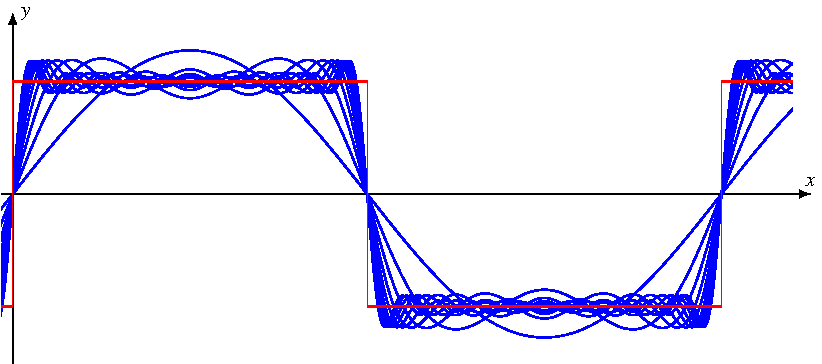
\includegraphics{chapters/010-skalarprodukt/images/fourierrechteck.pdf}
\caption{Approximation der Rechteckfunktion (rot) durch eine Folge
von Partialsummen der Fourier-Reihe.
\label{buch:skalarprodukt:fig:fourierrechteck}}
\end{figure}%
Die Supremum-Norm auf dem Raum der stetigen Funktionen hat den
Begriff der gleichmässig konvergenten Funktionenfolgen ergeben.
Cauchy-Folgen von stetigen Funktionen in der Supremum-Norm konvergieren
wieder gegen eine stetige Funktione.
Ist eine Funktion nicht stetig, lässt Sie sich im Sinne der Supremum-Norm
nicht durch stetige Funktionen approximieren.
Andererseits hat Fourier gezeigt, wie man technische wichtige Funktionen
wie die Rechteckfunktion durch trigonometrische Polynome
\begin{equation}
f_n(x)
=
\frac{4}{\pi} \sum_{k=0}^n \frac{\sin kx}{k}
=
\frac{4}{\pi} \biggl(
\sin x
+
\frac{\sin 3x}{3}
+
\frac{\sin 5x}{5}
+
\frac{\sin 7x}{7}
+
\ldots
\biggr)
\label{buch:skalarprodukt:eqn:rechteckreihe}
\end{equation}
approximieren kann.
Diese sind alle stetig und kommen der Rechteckfunktion in jedem Punkt,
in dem die Funktion stetig ist, beliebig nahe.
An den Stellen $x = n\pi$ hat die Grenzfunktion eine Sprungstelle,
die approximierenden Funktionen haben dort immer Abstand $1$
(siehe Abbildung~\ref{buch:skalarprodukt:fig:fourierrechteck}).
Die Folge ist also keine Cauchy-Folge und sie konvergiert nicht im
Sinne der Supremum-Norm.
Für solche Anwendungen muss eine besser geeignete Norm gefunden werden,
in der die Folge konvergiert.

%
% Skalarprodukt von Funktion
%
\subsubsection{Die $L^1$-Norm einer Funktion}
Die Supremum-Norm sieht nur den grössten Wert, die Konvergenz der Folge
\eqref{buch:skalarprodukt:eqn:rechteckreihe} ist aber nicht gleichmässig,
die maximale Abweichung ist immer $1$.
Gesucht ist eine Norm, die für die Folge
\eqref{buch:skalarprodukt:eqn:rechteckreihe} 
nur im Mittel eine Abweichung feststellt.
Für die Berechnung des Mittelwerts kann das Integral verwendet werden:

\begin{definition}
\label{buch:skalaprodukt:definition:l1norm}
Für eine stetige Funktion $X\to\mathbb{R}$, für die $x\mapsto |f(x)|$
integrierbar ist, heisst
\begin{equation}
\|f\|_1 = \int_X |f(x)|\,dx
\label{buch:skalarprodukt:eqn:l1norm}
\end{equation}
die {\em $L^1$-Norm} der Funktion $f$.
\end{definition}

Die $L^1$-Norm ist tatsächlich eine Norm, wir verifizieren die
definierenden Eigenschaften einer Norm.
\begin{enumerate}
\item
Definit: Sei $f$ eine stetige Funktion mit $\|f\|_1=0$
Wäre $f\ne 0$, dann gäbe es einen Punkt $x_0\in X$ mit $f(x_0) \ne 0$.
Da $f$ stetig ist, ist $f|(x)| > \frac12|f(x_0)|$ für $x$ in einer
$\delta$-Umgebung von $x_0$.
Dann folgt für die $L^1$-Norm
\begin{align*}
\|f\|_1
=
\int_X |f(x)|\,dx
\ge
\frac12 |f(x_0)| \cdot \delta 
> 0.
\end{align*}
Dies widerspricht der Annahme, dass $\|f\|_1=0$ ist, also muss $f=0$ sein.
\item
Homogeneität folgt durch direkte Rechnung
\[
\|\lambda f\|_1
=
\int_X |\lambda f(x)|\,dx
=
|\lambda|
\int_X |f(x)|\,dx
=
|\lambda| \cdot \|f\|.
\]
\item
Die Dreiecksungleichung folgt aus
\[
\|f+g\|_1
=
\int_X |f(x) + g(x)|\,dx
\le
\int_X |f(x)| + |g(x)|\,dx
=
\int_X |f(x)| + \int_X |g(x)|\,dx
=
\|f\|_1 + \|g\|_1.
\]
\end{enumerate}

Die $L^1$-Norm ist etwas ``schwächer'' als die Supremum-Norm im
folgenden Sinne.
Eine in der Supremum-Norm konvergente Funktionenfolge auf einem
kompakten Definitionsbereich $X$ ist auch in der $L^1$-Norm konvergent.
Zur Unterscheidung der verschiedenen Normen werden wir in Zukunft die
Supremum-Norm manchmal auch als $\|f\|_{\infty} = \|f\|$ schreiben.

\begin{satz}
Ist $X$ eine kompakte Teilmenge von $\mathbb{R}$ und $f_n$ eine
in der Supremum-Norm konvergente Folge stetiger Funktionen $f_n$,
dann ist $f_n$ auch in der $L^1$-Norm konvergent.
\end{satz}

\begin{proof}
Konvergenz in der Supremum-Norm bedeutet, dass für jedes $\varepsilon>0$
ein $N>0$ existiert derart, dass $|f_n(x)-f(x)|<\varepsilon$ für alle
$x\in X$ und alle $n>N$.
Für die $L^1$-Norm gilt dann
\begin{align*}
\|f_n-f\|_1
&=
\int_X |f_n(x) - f(x)|\,dx
\le
\int_X \varepsilon \,dx
=
\varepsilon \int_X \,dx
=
\varepsilon \operatorname{vol}(X).
\end{align*}
Da für einen kompakten Definitionsbereich $\operatorname{vol}(X)<\infty$
gilt, bedeutet dies, dass die $\|f_n-f\|_1\to 0$, dass also $f_n$ in
der $L^1$-Norm konvergiert.
\end{proof}

\begin{beispiel}
Die Folge $f_n(x)$ von \eqref{buch:skalarprodukt:fig:fourierrechteck}
konvergiert tatsächlich in der $L^1$-Norm auf dem Intervall $[0,2\pi]$.
Zwar ist $f_n$ nicht gleichmässig konvergent, aber fast.
Man kann zeigen, dass für jedes $\delta>0$, die Funktionen
$f_n(x)$ in Punkten $x$, die weiter als $\delta$ von den
Punkten $k\pi$ mit $k\in\mathbb{Z}$, gleichmässig konvergieren.
Innerhalb einer $\delta$-Umgebung der Vielfachen von $\pi$ ist die
$f_n(x)-f(x)$ beschränkt.
Die genaue Schranke ist nicht wichtig, wir nennen sie $M$ und bekommen
\[
|f_n(x)-f(x)|
\le M
\quad\forall x\in X.
\]
Ausserhalb einer kleinen Umgebung konvergiert die Folge gleichmässig,
zu jedem $\varepsilon>0$ gibt es also ein $N>0$ derart, dass
\[
|f_n(x)-f(x)|<\varepsilon
\]
für $x$ weiter als $\delta$ von $k\pi$ entfernt.
Für die $L^1$-Norm folgt dann
\begin{align*}
\|f_n-f\|_1
&=
\int_0^{2\pi} |f_n(x)-f(x)|\,dx
\\
&=
\int_0^\delta |f_n(x)-f(x)|\,dx
+
\int_\delta^{\pi-\delta} |f_n(x)-f(x)|\,dx
+
\int_{\pi-\delta}^{\pi+\delta} |f_n(x)-f(x)|\,dx
\\
&\qquad
+
\int_{\pi+\delta}^{2\pi-\delta} |f_n(x)-f(x)|\,dx
+
\int_{2\pi-\delta}^{2\pi} |f_n(x)-f(x)|\,dx
\\
&\le
\delta M
+
\varepsilon (\pi -2\delta)
+
2\delta M
+
\varepsilon (\pi -2\delta)
+
\delta M
\le
4\delta M + 2\pi\varepsilon
\end{align*}
für $n>N$.
Dadurch, dass man $\delta$ und $\varepsilon$ klein macht, kann man
also immer ein $N$ finden, so dass $\|f_n-f\|_1$ beliebig klein wird
für $n>N$.
Damit ist gezeigt, dass die Folge $f_n$ in der $L^1$-Norm konvergiert.
\end{beispiel}

Das Beispiel zeigt, dass die $L^1$-Norm eine schwäre Form der Konvergenz
ist, die eine erweiterte Klasse von Funktionen durch stetige Funktionen
zu approximieren erlaubt.

%
% Das $L^2$-Skalarprodukt
%
\subsubsection{Das $L^2$-Skalarprodukt}
Die $L^1$-Norm ist weniger strikt als die Supremum-Norm, aber sie ist
immer noch recht weit von der Intuition entfernt, die wir von der
Entfernungsmessung in der Geometrie haben, die von einem Skalarprodukt
herrühren.
Das Beispiel~\ref{buch:skalarprodukt:cauchyschwarz:beispiel:skalarprodukt}
weist den Weg, mit dem wir eine Norm für stetige Funktionen gewinnen
können, die von einem Skalarprodukt herkommt.

\begin{definition}
\label{buch:skalarprodukt:funktionraeume:definition:skalarprodukt}
Das {\em Skalarprodukt} stetiger Funktionen auf $X\subset \mathbb{R}$
ist definiert durch
\begin{equation}
\langle f,g\rangle
=
\int_X f(x)g(x)\,dx.
\label{buch:skalarprodukt:funktionraeume:eqn:skalarprodukt}
\end{equation}
\end{definition}

Es genügt nachzurechnen, dass $\langle f,g\rangle$ die Eigenschaften
eines Skalarproduktes hat, dann folgt die Dreiecksungleichung automatisch.
Zunächst ist klar,
dass~\eqref{buch:skalarprodukt:funktionraeume:eqn:skalarprodukt}
bilinear ist:
\begin{align*}
\langle \lambda f_1+\mu f_2,g\rangle
=
\int_X (\lambda f_1(x) + \mu f_2(x)) g(x)\,dx
&=
\lambda\int_Xf_1(x)g(x)\,dx + \mu\int_X f_2(x)g(x)\,dx
\\
&=
\lambda\langle f_1,g\rangle + \mu\langle f_2,g\rangle
\\
\langle f,\lambda g_1+\mu g_2\rangle
=
\int_X f(x)(\lambda g_1(x)+\mu g_2(x))\,dx
&=
\lambda\int_X f(x)g_1(x)\,dx + \mu\int_X f(x)g_2(x)\,dx
\\
&=
\lambda\langle f,g_1\rangle + \mu\langle f,g_2\rangle.
\end{align*}
Die Bilinearform ist aber auch positiv definit: Für eine stetige
Funktion $f(x)$ gilt
\[
\langle f,f\rangle
=
\int_X f(x)^2\,dx \ge 0.
\]
Da auch $f(x)^2$ eine stetige Funktion ist,
verschwindet das Integral genau dann, wenn $f(x)=0\;\forall x\in X$ ist.

Die zum Skalarprodukt gehörige Norm 
\[
\|f\|_2
=
\int_X |f(x)|^2\,dx
\]
heisst auch die {\em $L^2$-Norm}.

%
% Nicht kompakte Definitionsbereiche
%
\subsubsection{Nicht kompakter Definitionsbereich}
Für stetige Funktionen auf einem kompakten Definitionsbereich scheinen
die drei Normen $\|\;\cdot\;\|_\infty$, $\|\;\cdot\;\|_1$ und
$\|\;\cdot\;\|_2$ zu den gleichen Konvergenzbegriffen zu führen.
In diesem Abschnitt soll gezeigt werden, dass dies für nicht kompakte
Definitionsbereiche nicht mehr gilt.
Nicht einmal die Menge der Funktionen, die eine endliche Norm haben,
ist gleich.

\begin{beispiel}
Auf dem Definitionsbereich $X=(0,1]$ hat die Funktion
$f(x)=\log x$ endliche $L^1$-Norm aber unendliche Supremum-Norm.

\medskip
\noindent
Wegen $\lim_{x\to 0+}\log x = -\infty$ folgt $\|\log\|=\infty$.
Für die $L^1$-Norm folgt mit der Substitution $y=\log x$ und
$dy = dx/x$ oder $dx = e^y\,dy$
\begin{align*}
\|\log\|_1
&=
\int_0^1|\log x|\,dx
=
-\int_0^1\log x\,dx
=
-\int_{-\infty}^0 e^y\,dy
=
-\biggl[ e^y \biggr]_0^{-\infty}
=
1.
\end{align*}
Insbesondere ist die $L^1$-Norm beschränkt.
\end{beispiel}

\begin{beispiel}
Auf dem Definitionsbereich $X=[1,\infty)$ hat die Funktion
$f(x)=1/x$ endliche $L^2$-Norm aber unendlich $L^1$-Norm.

\medskip
\noindent
Die Integrale für die Normen ergeben:
\begin{align*}
\|f\|_1
&=
\int_1^\infty \frac{1}{x}\,dx
&
\|f\|_2^2
&=
\int_1^\infty \frac{1}{x^2}\,dx
\\
&=\biggl[\log x\biggr]_1^\infty
&
&=\biggl[-\frac{2}{x}\biggr]_1^\infty
\\
&=\infty
&
&=2.
\end{align*}
Insbesondere ist die $L^1$-Norm unbeschränkt, die $L^2$-Norm dagegen
beschränkt.
\end{beispiel}

\begin{satz}
Eine stetige Funktion auf einem beschränkten Definitionsbereich $X$
mit endlicher $L^2$-Norm hat auch endliche $L^1$-Norm.
\end{satz}

\begin{proof}[Beweis]
Aus der Cauchy-Schwarz-Ungleichung folgt
\begin{align*}
\int_X |f(x)|\,dx
&=
\langle |f|, 1\rangle
\le
\|f\|_2\cdot \|1\|_2.
\end{align*}
Nach Voraussetzung an die Funktion $f$ ist der erste Faktor beschränkt,
der zweite Faktor ist $\operatorname{vol}(X)$ und nach Voraussetzung
auch beschränkt.
\end{proof}

Die Beispiele zeigen, dass die Existenz der Normen selbst für stetige
Funktionen für nicht kompakten Definitionsbereich nicht garantiert ist.
Die Erweiterung auf nicht stetige Funktionen kann muss daher beschränkt
werden auf eine Klasse von Funktionen, für die die entsprechende Norm
existiert.
Das kann bedeuten, dass nicht alle stetigen Funktionen in Betracht 
kommen und dass neue Funktionen, die nicht stetig sind, als
Grenzwerte auftreten können.

%
% Grenzen des Riemann-Integrals
%
\subsection{Grenzen des Riemann-Integrals}
In den vorangegangenen Rechnungen sind wir immer vom Riemann-Integral
ausgegangen, welches man im Analysisunterricht als erstes kennenlernt.
Man zeigt dort, dass es für stetige Funktionen existiert und für
gleichmässig konvergente Folgen von Funktionen der Grenzwert des
Integrals mit dem Integral des Grenzwertes übereinstimmt:
\[
\int_X \lim_{n\to\infty} f_n(x)\,dx
=
\lim_{n\to\infty}
\int_X f_n(x)\,dx
\]
Der vorangegangene Abschnitt hat gezeigt, dass wir die Klasse der
Funktionen ausdehnen müssen auf Funktionen, die nicht stetig sind,
für die aber immer noch die $L^1$- oder die $L^2$-Norm existiert.
Hier zeigen sich die Schwächen des Riemann-Integrals.
In diesem Abschnitt soll an Beispielen gezeigt werden, was schief
gehen kann, und wie das Problem gelöst werden kann.

%
% Abzählbar viele Stetigkeitsstellen
%
\subsubsection{Abzählbar viele Unstetigkeitsstellen}
Wir konstruieren eine Funktionenfolge von Riemann-integrierbaren 
Funktionen, die alle das Integral $0$ haben, deren Grenzfunktion
aber nicht mehr Riemann-integrierbar ist.

Die rationalen Zahlen im Intervall $[0,1]$ sind abzählbar, d.~h.~es
gibt eine Folge $n\mapsto q_n\in[0,1]\cap\mathbb{Q}$, in der jede
rationale Zahl im Intervall vorkommt.
Aus der Folge $q_n$ konstruieren wir jetzt die Folge von Funktionen
\[
f_n(x)
=
\begin{cases} 
1&\qquad\text{$x$ ist einer der Werte $q_1,q_2,\ldots,q_n$}\\
0&\qquad\text{sonst}.
\end{cases}
\]
Die Funktion $f_n(x)$ ist also an genau $n$ Stellen von $0$ erschieden
und hat dort den Wert $1$.
Das Riemann-Integral ``sieht'' endlich viele Sprungstellen nicht,
die Funktionen $f_n$ sind also alle Riemann-integrierbar und haben
das Integral
\[
\int_0^1 f_n(x)\,dx=0.
\]
Insbesondere ist auch
\[
\lim_{n\to\infty}\int_0^1 f_n(x)\,dx = 0.
\]
Andererseits ist die Grenzfunktion
\begin{equation}
f(x)
=
\begin{cases}
1&\qquad\text{$x\in[0,1]\cap\mathbb{Q}$ ist rational}\\
0&\qquad\text{sonst, $x$ ist irrational.}
\end{cases}
\label{buch:skalarprodukt:funktionenraeume:eqn:ratfunk}
\end{equation}
Das Riemann-Integral der Funktion $f(x)$ existiert nicht.
Dazu müsste man ja für eine Unterteilung $0=x_0<x_1<\dots x_n=1$
die Riemann-Summen
\[
\overline{I}
=
\sum_{k=0}^{n-1}
(x_{k+1}-x_k) \sup_{x_k\le \xi \le x_{k+1}} f(\xi)
\qquad\text{und}\qquad
\underline{I}
=
\sum_{k=0}^{n-1}
(x_{k+1}-x_k) \inf_{x_k\le \xi \le x_{k+1}} f(\xi)
\]
berechnen, und sie müssten bei Verfeinerung der Unterteilung
gegeneinander konvergieren.
Aufgrund der Konstruktion der Funktion $f(x)$ ist aber
\[
\sup_{x_k\le \xi \le x_{k+1}} f(\xi) = 1
\qquad\text{und}\qquad
\inf_{x_k\le \xi \le x_{k+1}} f(\xi) = 0,
\]
sodass
$\overline{I}=1$ und $\underline{I}=0$ ist, ganz unabhängig von
der Unterteilung.

Der Riemannsche Integralbegriff muss also für die Zwecke der Approxmation
mit der $L^1$ oder $L^2$-Norm erweitert werden, so dass er sinnvoll mit
abzählbar vielen Unstetigkeitsstellen umgehenn kann.
Insbesondere sollte er als Integral der Funktion $f(x)$ 
von \eqref{buch:skalarprodukt:funktionenraeume:eqn:ratfunk}
den Wert $0$ liefern.

%
% Masse
%
\subsubsection{Masstheorie}
Gesucht wird also ein Integral, das für eine grössere Klasse von
Funktionen definiert ist und welches sich bezüglich Grenzwerten
besser verhält als das Riemann-Integral.
Das Integral ist nur dann nützlich, wenn es für viele Funktionen
die gleichen Werte ergibt.

Die einfachsten Funktionen, die wir integrieren wollen, sind die
{\em Indikatorfunktionen}, Funktionen, die durch eine Teilmenge
\index{Indikatorfunktion}
$A\subset X$ definiert sind durch
\[
1_A(x)
=
\begin{cases}
1&\qquad\text{für $x\in A$}\\
0&\qquad\text{sonst}.
\end{cases}
\]
Für ein Intervall der Länge $\lambda(A)$ ist
\[
\int_X 1_A(x)\,dx = \lambda(A).
\]
Für Mengen, die sich aus vielen Intervallen zusammensetzen, erwarten wir
die Summenformel
\[
A=\bigcup_{k=1}^\infty A_k,
\quad
A_k\cap A_j = \emptyset\;\forall k\ne j
\qquad\Rightarrow\qquad
\lambda(A) = \sum_{k=1}^\infty \lambda(A_k).
\]
Ausserdem sollte für eine Teilmenge $A\subset B$ der Inhalt der
Differenz $\lambda(A\setminus B)=\lambda(A)-\lambda(B)$ sein.

So entsteht eine Klasse von Mengen, denen sinnvoll ein Inhalt 
zugeordnet werden kann.
Solche Mengen heissen {\em messbar}.
Dazu gehören alle Intervalle, aber auch alle Differenzen und
abzählbaren Vereinigungen von Intervallen und messbaren Mengen
sind wieder messbar.
Die Klasse der messbaren Mengen ist also sehr gross.
Es braucht natürlich noch einiges an Arbeit, um zu zeigen, dass
eine widerspruchsfreie Definition der Funktion $\lambda(A)$
tatsächlich möglich ist, die jeder messbaren Menge einen
Inhalt zuordnet.
Eine solche Funktion heisst ein {\em Mass}, das aus der Intervalllänge
konstruierte Mass heisst auch das Lebesgue-Mass nach Henri Léon Lebesgue..
\index{Lebesgue-Mass}%
\index{Mass}%

Von besonderem Interesse sind Mengen, deren Inhalt $0$ ist.

\begin{definition}
\label{buch:skalarprodukt:funktionenraeume:definition:nullmenge}
Eine Nullmenge bezüglich des Masses $\lambda$ ist eine messbare
Menge $A$ mit Mass $\lambda(A)=0$.
\index{Nullmenge}
\end{definition}

Der Riemannsche Integralbegriff lässt bei der Bestimmung des Masses
nur endlich viele Intervalle zu. 
Die Menge $Q$ der rationalen Zahlen im Intervall $[0,1]$ ist abzählbar
unendlich.
In jeder beliebigen Umgebung einer reellen Zahl in $[0,1]$ findet man
rationale Zahlen in $Q$, eine Überdeckung der Menge der rationalen
Zahlen mit endlich vielen Intervallen enthält daher immer auch alle
reellen Zahlen, mit der möglichen Ausnahme von endlich vielen Zahlen.
Der Inhalt, den der Riemannsche Integralbegriff der Menge $Q$ zuordnen
muss, ist daher $1$.

Der neue Massbegriff erlaubt, die Menge mit abzählbar vielen messbaren
Mengen zu überdecken.
Sei $q_k$ eine Folge, die alle rationalen Zahlen in $Q$ durchläuft.
Zu jedem $k$ konstruieren wir das Intervall
\[
A_k = (q_k-\varepsilon2^{-k},q_k+\varepsilon2^{-k})
\]
mit Inhalt $\lambda(A_k) = 2\varepsilon2^{-k}$.
Es ist klar, dass die Intervalle $A_k$ die ganze Menge $Q$ überdecken,
also
\[
Q\subset \bigcup_{k=1}^\infty A_k.
\]
Der Inhalt der Menge $Q$ ist daher
\[
\lambda(Q)
\le
\sum_{k=1}^\infty \lambda(A_k)
=
\sum_{k=1}^\infty 2\varepsilon 2^{-k}
=
2\varepsilon
\sum_{k=1}^\infty 2^{-k}
=
2\varepsilon.
\]
Da $\varepsilon$ beliebig klein gewählt werden kann, folgt, dass
$\lambda(Q)=0$ sein muss.
Aus diesem Beispiel lässt sich erahnen, dass der Lebesguesche Massbegriff
mit Grenzwerten besser umgehen kann als der aus dem Riemannschen Integral
abgeleitete.

%
% Lebesgue-Integral
%
\subsubsection{Lebesgue-Integral}
Aus der Konstruktion eines Masses $\lambda$ kann jetzt die Konstruktion
eines Integrals an die Hand genommen werden.
Dazu werden Funktionen durch Stufenfunktionen approximiert, die
von der Form
\[
f(x) = \sum_{k=1}^\infty a_k 1_{A_k}(x)
\]
sind, wobei $A_k$ messbare Mengen sind.
Für solche Funktionen ist die naheliegende Definition des Integrals
\[
\int_X f(x)\,d\lambda(x)
=
\sum_{k=1}^\infty a_k \lambda(A_k).
\]
Der wesentliche Unterschied zur Riemannsschen Konstruktion ist,
dass nicht nur Intervalle zulässig sind sondern beliebige messbare Mengen.
Die Berechnung des Inhalts einer messbaren Mengen beinhaltet bereits
die Möglichkeit, Grenzwerte zu bilden.
Auch hier ist viel Arbeit notwendig um nachzuweisen, dass sich aus diesem
Ansatz ein widerspruchsfreier neuer Integralbegriff ergibt.
Das so konstruierte Integral heisst das {\em Lebesgue-Integral} und
\index{Lebesgue-Integral}%
wird zur Unterscheidung vom gewöhnlichen Riemannschen Integral und
wegen der Bedeutung des Masses $\lambda$, welches eine grosse Rolle
bei seiner Konstruktion spielt mit
\[
\int_X f(x) \,d\lambda(x)
\]
bezeichnet.

Beim Riemannschen Integral haben endliche Mengen und Mengen mit endlich
vielen Häufungspunkten Inhalt $0$.
Viele abzählbare Mengen haben dagegen positiven Inhalt.
Das Lebesguesche Mass gibt allen abzählbaren Mengen den Inhalt 0.

Unterscheiden sich zwei Funktionen $f$ und $g$ nur auf einer Nullmenge,
sagt man, sie seien {\em fast überall} gleich, geschrieben
\[
f(x) = g(x) \qquad \text{fast überall}.
\]
Zwei fast überall gleiche Funktionen haben das gleiche Integral, denn
\[
\int_X f(x)\,dx - \int_X g(x)\,dx
=
\int_X f(x)-g(x)\,dx
=
\int_X 0\,dx=0
\]
weil das Integral einer fast überall verschwindenden Funktion $0$ ist.

%
% Funktionsklassen
%
\subsubsection{Klassen von fast überall gleichen Funktionen}
Verwendet man die mit dem Lebesgque-Integral berechnete $L^1$- oder
$L^2$-Norm, dann können Funktionen nicht voneinander unterschieden werden,
die fast überall gleich sind.
Grenzwerte von Funktionenfolgen in der $L^1$- oder $L^2$-Norm sind
daher nur bis auf eine Nullmenge bestimmt.

\begin{definition}
Die Menge der Lebesgue-integrierbaren Funktionen auf dem Definitionsbereich
$X\subset\mathbb{R}$ wird mit
\[
\mathscr{L}^1(X)
=
\mathscr{L}^1_{\mathbb{R}}(X)
=
\left\{ f\colon X\to \mathbb{R}
\;\left|\;
\text{$f$ ist $\lambda$-integrierbar und $\int_X|f(x)|\,dx< \infty$}
\right.\right\}
\]
bezeichnet.
Entsprechend besteht $\mathscr{L}^2(X)$ aus den Funktionen $X\to \mathbb{R}$,
für die $|f(x)|^2$ integrierbar ist.
Sie heissen auch die {\em quadratintegrierbaren} Funktionen.
\end{definition}

Das Lebesgue-Integral kann Funktionen, die sich nur auf einer Nullmenge
verschieden sind, nicht unterscheiden. 
Daher ist es notwenig, solche Funktionen in Klassen zusammenzufassen:

\begin{definition}
Die Relation
\[
f\sim g
\qquad:\Leftrightarrow \qquad f(x) = g(x)\quad\text{fast überall}
\]
ist eine Äquivalenzrelation.
Die Menge der Äquivalenzklassen von Funktionen in $\mathscr{L}^1(X)$
bezüglich dieser Relation werden mit $L^1(X)$ bezeichnet, ebenso werden
die Äquivalenzklassen von $\mathscr{L}^2(X)$ bezüglich der Relation $\sim$
mit $L^2(X)$ bezeichnet.
\end{definition}

Mit den Funktionsklassen in $L^1(X)$ und $L^2(X)$ lässt sich genau
so rechnen, wie man es sicht gewohnt ist.
Für die Summe von Funktionen $f_1\sim f_2$ und $g_1\sim g_2$ gilt
\[
\left.
\begin{aligned}
f_1(x)&=f_2(x)&&\text{fast überall}\\
g_1(x)&=g_2(x)&&\text{fast überall}\\
\end{aligned}
\quad
\right\}
\qquad
\Rightarrow
\qquad
f_1(x)+g_1(x) = f_2(x)+g_2(x)\quad\text{fast überall},
\]
denn die Menge, auf der sich $f_1+f_2$ und $g_1+g_2$ unterscheiden
ist höchstens die Vereinigung der Mengen, auf denen sich $f_1$ und 
$f_2$ bzw.~$g_1$ und $g_2$ unterscheiden.
Die Vereinigung von Nullmengen ist aber wieder eine Nullmenge.

%
% Lebesgue-Integral
%
\subsubsection{Dominierte Konvergenz}
Die Entwicklung des Lebesgueschen Integrallbegriffs war motiviert
vom Wunsch, ein Integral zu erhalten, welches sich bezüglich
Konvergenz von Funktionenfolgen besser verhält.
Tatsächlich liefert die Theorie den folgenden zentralen Satz.

\begin{satz}[Dominierte Konvergenz]
\label{buch:skalarprodukt:satz:dominierte-konvergenz}
Sei $f_n$ eine auf dem Definitionsbereich $X$ punktweise konvergente
Folge Lebesgue-integrierbarer Funktionen mit Grenzfunktion 
\[
f(x) = \lim_{n\to \infty} f_n(x).
\]
Sei ausserdem $g$ eine Lebesgue-integrierbare Funktion mit
$|f_n(x)|<g(x)$ für alle $x\in X$.
Dann ist $f$ Lebesgue-integrierbar und es gilt
\[
\lim_{n\to\infty} \int_X f(x)\,d\lambda(x)
=
\int_X f(x)\,d\lambda(x)
\]
\end{satz}

Der Satz der dominierten Konvergenz von Lebesgue ersetzt also die
Bedingung der gleichmässigen Konvergenz, die beim Riemann-Integral
erfolgreich war, durch die viel schächere Bedingung, dass alle
Funktionen unterhalb einer gemeinsamen integrierbaren Funktion bleiben.
Dadurch wird verhindert, dass die Funktionen $f_n$ nach $\infty$
``ausbrechen'' kann und gegen eine Funktion konvergieren, die nicht
mehr integrierbar ist.


%
% Berechnung von Lebesgue-Integralen
%
\subsubsection{Berechnung von Lebesgue-Integralen}
Das Lebesque-Integral löst also die technischen Probleme, die das
Riemann-Integral manchmal bei Funktionenfolgen hat, die gegen ein
Grenzfunktion konvergieren, der man ein sinnvolles Integral im
Lebesgueschen Sinnen zuordnen kann.
Doch wie berechnet man ein Lebesgue-Integral?

Stetige Funktionen lassen sich beliebig genau durch Treppenfunktionen
approximieren.
Die Konvergenz des Lebesgue-Integrals für solche Funktionenfolgen
garantiert daher, dass das Lebesgue-Integral für stetige
Funktionen mit dem Riemann-Integral übereinstimmt.
Insbesondere braucht es keinen neuen Formalismus für die 
Berechnung von Integralen.
Auch für Funktionen, die an höchstens endlich vielen Stellen unstetig
sind, stimmt das Riemann-Integral mit dem Lebesgue-Integral überein.

Man soll sich daher das Lebesgue-Integral vor allem als eine 
Erweiterung des Integrals auf Funktionen vorstellen, die als Grenzwerte
von Folgen stetiger Funktionen im Sinne der $L^1$- oder der $L^2$-Norm
auftreten können.
Stetigkeit kann dabei verloren gehen, aber Konvergenzeigenschaften
wie die dominierte Konvergenz von
Satz~\ref{buch:skalarprodukt:satz:dominierte-konvergenz}
bleiben erhalten.




%
% 4-hilbertraum.tex
%
% (c) 2022 Prof Dr Andreas Müller, OST Ostschweizer Fachhochschule
%
\section{Hilbert-Raum
\label{buch:skalarprodukt:section:hilbertraum}}
\kopfrechts{Hilbert-Raum}
Ein Skalarprodukt stattet einen Vektorraum mit einer Norm aus.
Es ermöglicht auch, orthonormierte Vektoren zu finden.
In endlichdimensionalen Vektorräumen können so besonders nützliche
Basen konstruiert werden.
In den Funktionenräumen von
Abschnitt~\ref{buch:skalarprodukt:section:funktionenraeume},
die unendlichdimensional sind, kann der Orthonormalisierungsprozess
ohne Ende weitergeführt werden.
Im Gegensatz zu einem endlichdimensionalen Vektorraum bilden diese
orthonormierten Vektoren keine Basis, denn nicht jeder Vektor lässt
sich als Linearkombination schreiben.
Dies wird erst mit Hilfe von Reihenentwicklungen möglich, doch dazu
müssen Fragen der Konvergenz solcher Reihen geklärt werden.
Der in diesem Abschnitt eingeführte Begriff des Hilbert-Raumes tut dies.

%
% Prähilbertraum
%
\subsection{Prähilbertraum}
Die Funktionenräume, in denen wir harmonische Analysis betreiben wollen,
zeichnen sich durch das Vorhandensein eines Skalarproduktes aus.
Wir fassen diese Eigenaschaften im Begriff des Prähilbertraumes
zusammen.

\begin{definition}
Ein reeller Prähilbertraum ist ein reller Vektorraum mit einem
(reellen) Skalarprodukt.
\index{Prähilbertraum}%
Eine komplexer Prähilbertraum ist ein komplexer Vektorraum mit einem
sesquilinearen Skalarprodukt.
\end{definition}

\begin{beispiel}
Der endlichdimensionale reelle Vektorraum $\mathbb{R}^n$ ist ein
reller Prähilbertraum mit dem Skalarprodukt
\[
\langle u,v\rangle
=
\sum_{i=1}^n u_iv_i
\]
für Vektoren $u,v\in\mathbb{R}^n$.
\end{beispiel}

\begin{beispiel}
Der endlichedimensionale komplexe Vektorrau $\mathbb{C}$ ist ein
komplexer Prähilbertraum mit dem Skalarprodukt
\[
\langle u,v\rangle
=
\sum_{i=1}^n \overline{u}_iv_i
\]
für Vektoren $u,v\in\mathbb{C}^n$.
\end{beispiel}

Die Skalarprodukte in den Beispielen sind nicht die einzig möglichen
Skalarprodukte.
Alternative Skalarprodukte auf einem reellen Prähilbertraum können 
durch eine beliebige positiv definite Matrix $A$ durch
\[
\langle u,v\rangle_A
=
\sum_{i,j=1}^n u_ia_{ij}v_j
\]
definiert werden.
Wir schreiben die aus $\langle\;,\;\rangle_A$ abgeleitete Norm mit
$\normfunc_A$.
Solange unser primäres Interesse der Approximation von Funktionen gilt,
kommt es vor allem darauf an, dass die Norm, die aus dem Skalarprodukt
abgeleitet wird, zu den gleichen konvergenten Folgen führen.
Die Funktion $u\mapsto \|u\|_A$ ist stetig, sie hat daher auf der
Einheitskugel des Prähilbertraumes ein Maximum und eine Minimum,
welches wir mit $M$ bzw.~$m$ bezeichen.
Dann folgt, dass
\[
m\|u\|\le \|u\|_A\le M\|u\|
\]
für beliebige Vektoren $u\in\mathbb{R}^n$.
Daraus kann man jetzt ableiten, dass die beiden Normen $\normfunc$
und $\normfunc_A$ auf die gleichen Cauchy-Folgen und die gleichen
konvergenten Folgen führen.
Wir zeigen dies für Cauchy-Folgen:
\begin{enumerate}
\item
Sei $u_k$ eine Cauchy-Folge bezüglich der Norm $\normfunc$,
und $\varepsilon>0$.
Wir müssen zeigen, dass $u_k$ auch eine Cauchy-Folge ist bezüglich
der Norm $\normfunc_A$.
Da $u_k$ eine Cauchy-Folge bezüglich der Norm $\normfunc$ ist,
gibt es ein $N>0$ derart, dass
$\|u_k-u_l\|<\varepsilon/M$ für $k,l>N$.
Dann folgt aber
\[
\|u_k-u_l\|_A
\le
M\|u_k-u_l\|
<
M\frac{\varepsilon}{M}
=
\varepsilon
\]
für $k,l>N$.
Somit ist $u_k$ eine Cauchy-Folge bezüglich der Norm $\normfunc_A$.
\item
Ist umgekehrt  $u_k$ eine Cauchy-Folge bezüglich der Norm $\|\,\cdot\,\|_A$,
dann gibt es ein $N>0$ derart, dass $\|u_k-u_l\|_A<m\varepsilon$ ist für
$k,l>N$.
Dann folgt
\[
m\|u_k-u_l\|\le \|u_k-u_l\|_A < m\varepsilon
\qquad\Rightarrow\qquad \|u_k-u_l\|<\varepsilon
\]
für $k,l>N$, also ist $u_k$ auch eine Cauchy-Folge bezüglich der Norm
$\|\,\cdot\,\|$.
\end{enumerate}
In einem endlichdimensionalen Prähilbertraum hat die Wahl des Skalarproduktes
keinen Einfluss darauf, ob eine Folge eine Cauchy-Folge ist oder nicht.
Orthonormierte Vektoren werden natürlich im Allgemeinen nicht mehr
orthonormiert, dies ist jedoch ein Aspekt, dem wir uns erst später
zuwenden werden.

%
% Orthonormierte Vektoren
%
\subsection{Orthonormierte Vektoren in einem Prähilbertraum}
Der Gram-Schmidt-Orthogonalisierungsprozess kann auf eine beliebige
\index{Gram-Schmidt}%
linear unabhängige Menge von Vektoren in einem Prähilbertraum angewendet
werden.
Aus den linear unabhängigen Vektoren $a_1,a_2,\dots$ werden die
orthonormierten Vektoren
\begin{align*}
b_1
&=
\frac{a_1}{\|a_1\|}
\\
b_2
&=
\frac{
a_2 - \langle b_1,a_2\rangle b_1
}{
\|a_2 - \langle b_1,a_2\rangle b_1\|
}
\\
&\phantom{i}\vdots
\\
b_n
&=
\frac{\displaystyle
a_n - \sum_{k=1}^{n-1} \langle b_k,a_n\rangle b_k
}{\displaystyle
\biggl\|a_n - \sum_{k=1}^{n-1} \langle b_k,a_n\rangle b_k\biggr\|
}.
\end{align*}

In einem endlichdimensionalen Vektorraum der Dimension $n$ bricht
der Prozess ab, sobald eine orthonormierte Basis $b_1,\dots,b_n$
aus $n$ Vektoren gefunden wurde.
Jeder andere Vektor $v$ lässt sich dann als Linearkombination
\begin{equation}
v
=
\langle b_1,v\rangle b_1 + \langle b_2,v\rangle b_2 + \dots
=
\sum_{k=1}^n \langle b_1,v\rangle b_1
\label{buch:skalarprodukt:hilbertraum:synthese}
\end{equation}
schreiben.
Da die Summe auf der rechten Seite endlich ist, entstehen keine
Bedenken bezüglich Konvergenz, wie das bei einer unendlichen
Reihe der Fall wäre.

%
% Vollständigkeit
%
\subsection{Vollständigkeit}
In einem unendlichdimensionalen Prähilbertraum bricht der
Orthogonalisierungsprozess nicht ab, es gibt immer noch einen
linear unabhängigen Vektor, der nicht in dem von den bereits
gefundenen Vektoren aufgespannten Raum liegt.
Die Summe~\ref{buch:skalarprodukt:hilbertraum:synthese} wird dann
eine unendliche Summe, die nur im Sinne eines Grenzwertes der
Partialsummenfolge
\begin{equation*}
s_n = \sum_{k=1}^n \langle b_k,v\rangle b_k
\end{equation*}
ausgewertet werden kann.
Man darf zwar aufgrund der Konstruktion aus $v$ davon ausgehen,
dass $s_n$ gegen $v$ konvergiert,
aber für eine beliebige Folge von Koeffizienten $c_k$ ist nicht
garantiert, dass die Summe
\[
\sum_{k=1}^\infty c_kb_k
=
\lim_{n\to\infty} \sum_{k=1}^n c_kb_k
\]
einen Grenzwert hat.
Ein nützliche Theorie kann nur entstehen, wenn gefordert wird,
dass jede Cauchy-Folge des Prähilbertraums tatschächlich konvergiert.

\begin{definition}
Ein Prähilbertraum heisst {\em Hilbert-Raum}, wenn er vollständig ist.
\end{definition}

Endlichdimensionale Vektorräume über sind automatisch vollständig,
da gibt es also gar keinen Unterschied zwischen Prähilbertraum und
Hilbert-Raum.
Das folgende Beispiel zeigt, dass dies für unendlichdimensionale
Hilbert-Räume nicht mehr zutrifft.

\begin{beispiel}
\label{buch:skalarprodukt:hilbertraum:bsp:sinreihe}
Der Funktionenraum
\(
C_{\mathbb{R}}([-\pi,\pi])
\)
der stetigen Funktionen auf dem Intervall $[-\pi,\pi]$ wird mit
dem Skalarprodukt
\[
\langle f,g\rangle
=
\int_{-\pi}^\pi f(x)g(x)\,dx
\]
zu einem Prähilbert-Raum.
Die Summanden der Reihe~\eqref{buch:skalarprodukt:eqn:rechteckreihe} 
sind Sinus-Funktionen, von denen wir später zeigen werden, dass sie
orthogonal sind.
Seien $s_n(x)$ die Partialsummen der Reihe, also
\begin{equation}
s_n(x) = \frac{4}{\pi}\sum_{k=0}^n \frac{\sin (2k+1)x}{2k+1},
\label{buch:skalarprodukt:hilbertraum:eqn:sn}
\end{equation}
dann kann man auch die Norm $\|s_n-s_m\|$, es gilt nämlich
\begin{equation}
\|s_n-s_m\|
=
\biggl\|
\frac{4}{\pi}
\sum_{k=m}^n \frac{\sin (2k+1)x}{2k+1}
\biggr\|,
\label{buch:skalarprodukt:hilbertraum:eqn:snsm}
\end{equation}
wobei wir $n>m$ angenommen haben, was wir ohne Beschränkung der 
Allgemeinheit tun dürfen.
Die Norm eines einzeln Terms ist
\begin{align}
\|\sin rx\|^2
&=
\int_{-\pi}^\pi \sin^2 rx\,dx
=
\int_{-\pi}^\pi \frac12 - \frac{\cos rx}{2}\,dx
=
\int_{-\pi}^\pi \frac12\,dx - \int_{-\pi}^\pi \frac{\cos rx}{2}\,dx.
\notag
\intertext{Der zweite Term ist ein Integral über eine Periode des
Integranden und verschindet daher.
Der erste Term ergibt daher}
\|\sin rx\|^2
&= \pi.
\intertext{Für die Terme der Summe
\eqref{buch:skalarprodukt:hilbertraum:eqn:sn}
folgt daher}
\biggl\|
\frac{\sin{2k+1}x}{2k+1}
\biggr\|^2
&=
\frac{\pi}{(2k+1)^2}.
\notag
\intertext{Für die Differenz
\eqref{buch:skalarprodukt:hilbertraum:eqn:snsm} finden wir daher}
\|s_n-s_m\|^2
\notag
&=
\frac{16}{\pi^2}
\sum_{k=m}^m \frac{\pi}{(2k+1)^2}
=
\frac{16}{\pi}
\sum_{k=m}^m \frac{1}{(2k+1)^2}.
\label{buch:skalarprodukt:hilbertraum:eqn:bsprest}
\end{align}
Da aus dem Analysisunterricht bekannt ist, dass die Reihe $\sum_k\frac1{k^2}$
konvergiert, kann die rechte Seite von 
\eqref{buch:skalarprodukt:hilbertraum:eqn:bsprest}
beliebig klein gemacht werden, die 
Reihe~\eqref{buch:skalarprodukt:eqn:rechteckreihe} 
ist also eine Cauchy-Folge im Prähilbertraum $C_{\mathbb{R}}([-\pi,\pi])$.
Die Grenzfunktion ist die Rechteckfunktion von
Abbildung~\ref{buch:skalarprodukt:fig:fourierrechteck}, sie ist nicht
stetig.
Wir haben also eine Cauchy-Folge im Prähilbertraum 
$C_{\mathbb{R}}([-\pi,\pi])$ gefunden, die darin nicht konvergiert.
\end{beispiel}

%
% Hilbert-Basis
%
\subsection{Hilbert-Basis}
Sei jetzt $H$ ein Hilbert-Raum.
Führt man wieder die Konstruktion einer orthonormierten Basis durch,
entsteht eine Menge $\mathcal{B}=\{b_1,b_2,\dots\}$ orthonormierter
Vektoren.
In einem unendlichdimensionalen Hilbert-Raum ist $\mathcal{B}$ eine
undendliche Menge.
Die Vollständigkeit des Hilbert-Raumes garantiert, dass jede
Cauchy-Folge konvergiert, insbesondere können wir zu jedem beliebigen
Vektor $v$ die Koeffizienten $c_k=\langle b_k,v \rangle$ bestimmen
und versuchen, mit der
Summe~\eqref{buch:skalarprodukt:hilbertraum:synthese}
den Vektor zurückzugewinnen.
Vollständigkeit garantiert zwar die Konvergenz gegen einen Grenzwert
\[
v_0 = \sum_{k=1}^\infty c_k b_k,
\]
aber es gibt keine Garantie, dass $v=v_0$ ist.

\begin{beispiel}
Die Funktionen
\[
b_k(x) = \sin (2k+1)x
\qquad\text{mit}\quad
k\in \mathbb{N}
\]
wurden in Beispiel~\ref{buch:skalarprodukt:hilbertraum:bsp:sinreihe}
die Rechteckfunktion synthetisiert.
Doch reichen diese Funktionen nicht aus, um alle Funktionen auf
dem Intervall $[-\pi,\pi]$ zu synthetisieren.

Für die konstante Funktion $v(x)$ sind die Koeffizienten
\[
\langle v,b_k\rangle
=
\int_{-\pi}^\pi v(x)b_k(x)\,dx
=
\int_{-\pi}^\pi \sin (2k+1)x\,dx
=
0,
\]
die Summe
\[
v_0
=
\sum_{k=0}^\infty
c_k
b_k(x)
=
0
\]
verschwindet also, $v\ne v_0$.
\end{beispiel}

Wir berechnen das Skalarprodukt 
\[
\langle v-v_0,b_k\rangle
=
\langle v,b_k\rangle
-
\biggl\langle \sum_{l=1}^\infty c_lb_l,b_k\biggr\rangle
=
c_k - \sum_{l=1}^\infty c_l\langle b_l,b_k\rangle
=
c_k - \sum_{l=1}^\infty c_l\delta_{lk}
=
c_k-c_k=0.
\]
Der Vektor $v-v_0$ muss also orthogonal sein zu allen Vektoren
$b_k$.
Die Menge der Vektoren $b_k$ kann also vergrössert werden um einen
weiteren Vektor, der zu allen vorhandenen Vektoren orthogonal ist.

\begin{satz}
Eine Menge von orthogonalen Vektoren in einem Prähilbertraum ist linear 
unabhängig.
\end{satz}

\begin{proof}[Beweis]
Angenommen, die orthogonalen Vektoren  $a_1,\dots,a_n$ sind linear
abhängig.
Dann gibt es Zahlen $\lambda_i$, die nicht alle $=0$ sind und derart,
dass
\[
\sum_{k=1}^n \lambda_ka_k
=
\lambda_1 a_1 + \ldots + \lambda_n a_n
=
0.
\]
Das Skalarprodukt mit $a_k$ ergibt
\[
0
=
\langle a_k,\lambda_1a_1 +\ldots + \lambda_na_n\rangle
=
\lambda_1
\langle a_k,a_1\rangle
+
\ldots
+
\lambda_n
\langle a_k,a_n\rangle
=
\lambda_k \|a_k\|^2
\]
für alle $k=1,\dots,n$.
Da die Vektoren $a_k\ne 0$ sind folgt, dass $\lambda_k=0$ sein muss
für alle $k=1,\dots,n$, im Widerspruch zur Voraussetzung, dass die
$\lambda_k$ nicht alle verschwinden.
Der Widerspruch zeigt, dass die Annahme der linearen Abhängigkeit
falsch ist.
\end{proof}

In einem endlichdimensionalen Prähilbertraum findet man immer eine
orthonormierte Basis, aus der sich jeder Vektor linear kombinieren
lässt.
In einem unendlichdimensionalen Raum muss dieser Begriff etwas 
erweitert werden.

\begin{definition}
Eine {\em Hilbert-Basis} des Hilbert-Raumes $H$ ist eine Menge von orthonormalen
\index{Hilbert-Basis}%
Vektoren $b_k\in H$, $k\in \mathbb{N}$ derart, für jeden Vektor $v\in H$
die Reihe 
\[
\sum_{k\in\mathbb{N}} \langle b_k,v\rangle b_k
\]
konvergiert und die Summe $v$ hat.
\end{definition}

Auf eine Hilbert-Basis ist die Inuition anwendbar, die man von 
einer orthonormierten Basis eines endlichdimensionalen Prählibertraumes
hat.

\begin{definition}
\index{separabel}%
Ein Hilbert-Raum, der eine Hilbert-Basis besitzt, heisst {\em separabel}.
\end{definition}

Nicht separable Hilbert-Räume sind deutlich grösser.
In einem nicht separable Hilbert-Raum ist es nicht möglich, alle Vektoren
aus einer Folge von orthonormierten Vektoren linear zu kombinieren.
Dies verträgt sich nicht mit der Intuition, die in endlichdimensionalen
Vektorräumen entstanden ist.
Separabilität ist eine Art ``Endlichkeitseigenschaft''.
Man findet sie zum Beispiel bei den $L^2$-Räumen mit kompaktem
Definitionsgebiet.
Kompaktheit kann als eine topologische
Endlichkeitseigenschaft angesehen werden.
Es lassen sich aber auch nicht separable Hilbert-Räume konstruieren,
zum Beispiel sogenannte fastperiodische Funktionen.
\index{fastperiodische Funktionen}%
Für unsere Anwendungen sind nicht separable Hilbert-Räume jedoch nicht
notwendig und wir können im folgenden annehmen, dass alle Hilbert-Räume
separabel sind und somit eine Hilbert-Basis haben.

%
% Der Hilbert-Raum $l^2$
%
\subsection{Der Hilbert-Raum $l^2$}
Die abstrakte Definition eines separablen Hilbert-Raumes suggeriert,
dass es sehr viele verschiedene Hilbert-Räume geben könnte.
Dem ist aber nicht so, ein Hilbert-Raum ist eine ziemlich starre Struktur.
In diesem Abschnitt konstrieren wir zunächst den besonders übersichtlichen
separablen Hilbert-Raum $l^2$ und zeigen anschliessend, dass sich jeder
separable Hilbert-Raum isometrisch auf $l^2$ abbilden lässt.

\begin{satz}
Der Vektorraum der unendlichen Folgen
\[
l^2_{\mathbb{R}}
=
\biggl\{
(x_0,x_1,\dots)
\in
\mathbb{R}^{\mathbb{N}}
\,\bigg|\,
\sum_{i=0}^\infty x_i^2<\infty\biggr\}
\}
\]
mit dem Skalarprodukt
\[
\langle x,y\rangle_2
=
\sum_{k=0}^\infty x_ky_k
\]
ist ein separabler Hilbert-Raum.
\end{satz}

\begin{proof}[Beweis]
Die Standardbasis des Vektorraums $l^2$ besteht aus den Vektoren $e_i$
mit $i\in\mathbb{N}$ mit 
\begin{align*}
e_0 &= (1,0,0,0,\dots)
\\
e_1 &= (0,1,0,0,\dots)
\\
e_2 &= (0,1,0,0,\dots)
\\  &\;\vdots
\end{align*}
Es ist klar, dass die Vektoren $e_i$ orthonormiert sind.
Wir müssen uns überlegen, dass jede Folge in $l^2$ durch Linearkombinationen
approximiert werden kann.
Wäre das nicht so, dann gäbe es einen von $0$ verschiedenen
Vektor $v=(v_0,v_1,v_2,\dots)\in l^2$, der auf allen Vektoren $e_i$
orthogonal ist.
Dann wäre aber $0=\langle v,e_i\rangle = v_i$, d.~h.~Vektor $v$ ist der
Nullvektor.
Dieser Widerspruch zeigt, dass die Vektoren $e_i$ eine Hilbert-Basis
bilden.
\end{proof}

Der Hilbert-Raum $l^2$ ist die einfachste, direkte Verallgemeinerung der
endlichdimensionalen Hilbert-Raume $\mathbb{R}^n$ mit dem Standardskalarprodukt.
Er ist aber auch der ``einzige'' separable Hilbert-Raum, alle Hilbert-Räume
lassen sich isometrisch auf $l^2$ abbilden.

\begin{satz}
\label{buch:skalarprodukt:hilbertraum:satz:phil2}
Ist $H$ ein separabler Hilbert-Raum, dann gibt es eine isometrische
lineare Abbildung $\varphi\colon H\to l^2$.
\end{satz}

\begin{proof}[Beweis]
Da $H$ separabel ist, gibt es eine Hilbert-Basis $b_0,b_1,b_2,\ldots\in H$
und $v$ ein beliebiger Vektor mit der Darstellung
\[
v = \sum_{k=0}^\infty c_kb_k.
\]
Das Skalarprodukt mit $b_k$ ist
\[
\langle b_i,v\rangle
=
\biggl\langle b_i,\sum_{k=0}^\infty c_kb_k\biggr\rangle
=
\sum_{k=0}^\infty c_k \underbrace{\langle b_i,b_k\rangle}_{\delta_{ik}}
=
c_i.
\]
Die Abbildung
\[
\varphi\colon H \to l^2
:
v \mapsto (\langle b_0,v\rangle,\langle b_1,v\rangle,\langle b_2,v\rangle,\dots)
=
(c_0,c_1,c_2,\dots)=c\in l^2
\]
ist linear und umkehrbar durch die Abbildung
\[
\varphi^{-1} \colon l^2 \to H
:
(c_0,c_1,c_2,\dots) \mapsto \sum_{k=0}^\infty c_k b_k.
\]
Die Norm von $v$ ist
\[
\|v\|^2
=
\biggl\|
\sum_{k=0}^\infty c_k b_k
\biggr\|^2
=
\sum_{k=0}^\infty c_k^2
=
\|c\|_2^2.
\qedhere
\]
\end{proof}

Man verliert also nichts, wenn man statt im Hilbert-Raum $H$ im
Hilbert-Raum $l^2$ rechnet.
Die später zu besprechende Fourier-Transformation ist genau
so eine Abbildung $\varphi$ wie in
Satz~\ref{buch:skalarprodukt:hilbertraum:satz:phil2}, wenn 
trigonometrische Funktionen als Basisfunktionen des Raumes
$L^2([-\pi,\pi])$ verwendet werden.
Die Tatsache, dass die Abbildung eine Isometrie ist, hat einen
speziellen Namen.

\begin{definition}
\label{buch:skalarprodukt:hilbertraum:def:parseval}
Die Identität
\[
\|v\|^2 = \|\varphi(v)\|_2^2
\]
heisst {\em Parseval-Gleichung}.
Aus der Polaridentität folgt dann auch die
{\em Parseval-Plancherel-Formel}
\[
\langle u,v\rangle_H
=
\langle\varphi(u),\varphi(v)\rangle_2
=
\sum_{k=0}^\infty
\langle b_k,u\rangle
\langle b_k,v\rangle.
\]
\end{definition}

Die endlichdimensionalen Hilbert-Räume können auf
natürliche Art in $l^2$ eingebettet werden, indem die Koordinaten
eines $n$-dimensionalen Vektors auf die ersten $n$-Komponenten der
Folge in $l^2$ abgebildet werden.
Aus dieser Idee lässt sich auch ein Prähilbertraum konstruieren,
in dem einfacher gerechnet werden kann.

\begin{definition}
\label{buch:skalarprodukt:hilbertraum:def:l0}
Sei 
\[
l_0
=
\{
x\in \mathbb{R}^{\mathbb{N}}
\mid
\text{$x_k\ne 0$ nur für endlich viele $k$}
\}
\]
der Vektorraum der Folgen, die nur endlich viele nicht verschwindende
Folgenglieder haben.
Die Standardbasisvektoren von $l^2$ sind alle in $l_0$.
\end{definition}

Da die Norm eines Elementes $x\in l_0$ eine endliche Summe ist,
ist $x\in l^2$ und damit $l_0\subset l^2$.
Jeder Vektor $v\in l^2$ kann aber beliebig genau durch einen Vektor
in $l_0$ approximiert werden.
Dazu konstruiert man die Folge
\bgroup
\def\el#1{\phantom{v_0}\llap{#1}}
\begin{align*}
x_0 &= (v_0,\el{0},\el{0},\el{0},\el{0},\dots) \in l_0\\
x_1 &= (v_0,v_1,\el{0},\el{0},\el{0},\dots) \in l_0\\
x_2 &= (v_0,v_1,v_2,\el{0},\el{0},\dots) \in l_0\\
x_3 &= (v_0,v_1,v_2,v_3,\el{0},\dots) \in l_0\\
    &\;\vdots
\end{align*}
\egroup
Die Differenz $x_n-v$ hat die Norm
\[
\|x_n-v\|^2
=
\sum_{k=n+1}^\infty v_k^2,
\]
die für $n\to\infty$ gegen $0$ geht.
Da es in $l^2$ Vektoren gibt, die nicht in $l_0$ drin sind, zeigt
dies, dass $l_0$ kein Hilbert-Raum ist, dass aber die Vervollständigung
von $l_0$ der Hilbert-Raum $l^2$ ist.

Der Prähilbert-Raum rechtfertigt, dass man in Anwendungen im Sinne
einer Approximation mit endlich vielen der Koeffizienten $c_k$
rechnen kann.
Im Kontext der Fourier-Theorie sind dies
die trigonometrischen Polynome, mit denen sich jede periodische
Funktion approximieren lässt.

%
% Der Hilbert-Raum $L^2$
%
\subsection{Der Hilbert-Raum $L^2$}
Der Vektorraum der stetigen Funktionen auf dem Intervall $[-\pi,\pi]$
mit dem bekannten Skalarprodukt ist ein Prähilbertraum.
Wir werden später zeigen, dass die Funktionen
\[
1, \cos kx \quad\text{und}\quad \sin kx
\qquad \text{mit $k\in\mathbb{N}$ und $ k\ge 1$}
\]
orthogonal sind bezüglich dieses Skalarproduktes.
Es wird sich zeigen, dass diese Funktionen nach geeigneter Normierung
eine Hilbert-Basis bilden von $L^2$ bilden.
Die in Satz~\ref{buch:skalarprodukt:hilbertraum:satz:phil2}
konstruierte Abbildung bezeichnen wir mit $\mathscr{F}:L^2([-\pi,\pi])\to l^2$.
Die Parseval-Plancherel-Formel besagt dann, dass man das Skalarprodukt
von Funktionen auch durch das Skalarprodukt der zugehörigen
Fourier-Koeffizienten berechnen kann:
\[
\langle f,g\rangle_{L^2{[-\pi,\pi]}}
=
\langle \mathscr{F}f,\mathscr{F}g\rangle_{l^2}.
\]
Die Fourier-Transformation formalisiert also die Erkenntnis, dass
man alle Fragen, die man mit Skalarprodukten beantworten kann, statt
mit Funktionen auch mit Skalarprodukten von Fourier-Koeffizienten
finden kann.

%
% Der Darstellungssatz von Riesz
%
\subsection{Der Darstellungssatz von Riesz}
Eine Linearform $l(x)$ auf dem Vektorraum $\mathbb{R}^n$ ist gegeben durch
die Werte $l(e_i)$ auf den Standardbasisvektoren.
Der Wert von auf $x=x_1e_1+\dots+x_ne_n$ ist dann
\[
l(x)
=
x_1l(e_1)+\dots+x_nl(e_n)
=
\begin{pmatrix}
l(e_1)\\\vdots\\l(e_n)
\end{pmatrix}
\cdot
\begin{pmatrix}
x_1\\\vdots\\x_n
\end{pmatrix}.
\]
Insbesondere lässt sich jede Linearform als Skalarprodukt mit einem 
geeigneten Vektor geschrieben werden.
Diese Eigenschaft gilt auch in einem Hilbert-Raum.

\begin{satz}[Riesz]
\label{buch:skalarprodukt:hilbertraum:satz:riesz}
Sei $H$ ein Hilbert-Raum und $l\colon H\to\mathbb{R}$ eine stetige
Linearform.
Dann gibt es eine $v\in H$ derart, dass $l(x) = \langle v,x\rangle$.
\end{satz}

Der Beweis dieser Eigenschaft kann man zum Beispiel in \cite{buch:wavelets}
finden.
Der Satz gilt natürlich auch in einem komplexen Hilbert-Raum.




%
% 5-sobolevraum.tex
%
% (c) 2022 Prof Dr Andreas Müller, OST Ostschweizer Fachhochschule
%
\section{Sobolev-Räume
\label{buch:skalarprodukt:section:sobolev}}
\kopfrechts{Sobolev-Räume}
Im Beispiel~\ref{buch:skalarprodukt:hilbertraum:bsp:sinreihe} haben 
wir eine Reihe kennengelernt, deren Partialsummen alle stetig sind,
da sie trigonometrische Polynome sind.
Doch die Grenzfunktion ist die Rechteckfunktion, die ganz offensichtlich
nicht stetig sind.
Die Norm des Hilbert-Raums $L^2$ ist offenbar nicht stark genug, die
Stetigkeit der Grenzfunktion sicherzustellen.

%
% tikztemplate.tex -- template for standalon tikz images
%
% (c) 2021 Prof Dr Andreas Müller, OST Ostschweizer Fachhochschule
%
\documentclass[tikz]{standalone}
\usepackage{amsmath}
\usepackage{times}
\usepackage{txfonts}
\usepackage{pgfplots}
\usepackage{csvsimple}
\usepackage{ifthen}
\usetikzlibrary{arrows,intersections,math}
\begin{document}
\def\skala{1}
\newboolean{draft}
\setboolean{draft}{false}
\begin{tikzpicture}[>=latex,thick,scale=\skala]

% add image content here
\def\s{12/(2*3.14159)}
\def\punkt#1#2{({(#1)*\s},{(#2)*\s})}

\draw[->] (-0.6,0) -- (13.2,0) coordinate[label={$x$}];
\draw[->] (0,{-1.72*\s}) -- (0,{1.8*\s}) coordinate[label={right:$y$}];

\begin{scope}
\clip (-0.6,{-1.8*\s}) rectangle (13.0,{1.8*\s});
\draw[color=blue] plot[domain=-20:420,samples=100]
	({(\x/360)*\s*2*3.14159},{(4/3.14159)*sin(\x)*\s});
\draw[color=blue] plot[domain=-20:420,samples=1000]
	({(\x/360)*\s*2*3.14159},{(4/3.14159)*(sin(\x)-sin(3*\x)/3)*\s});
\ifthenelse{\boolean{draft}}{}{
\draw[color=blue] plot[domain=-20:420,samples=1000]
	({(\x/360)*\s*2*3.14159},{(4/3.14159)*(sin(\x)-sin(3*\x)/(3*3)+sin(5*\x)/(5*5))*\s});
\draw[color=blue] plot[domain=-20:420,samples=1000]
	({(\x/360)*\s*2*3.14159},{(4/3.14159)*(sin(\x)-sin(3*\x)/(3*3)+sin(5*\x)/(5*5)-sin(7*\x)/(7*7))*\s});
\draw[color=blue] plot[domain=-20:420,samples=1000]
	({(\x/360)*\s*2*3.14159},{(4/3.14159)*(sin(\x)-sin(3*\x)/(3*3)+sin(5*\x)/(5*5)-sin(7*\x)/(7*7)+sin(9*\x)/(9*9))*\s});
\draw[color=blue] plot[domain=-20:420,samples=1000]
	({(\x/360)*\s*2*3.14159},{(4/3.14159)*(sin(\x)-sin(3*\x)/(3*3)+sin(5*\x)/(5*5)-sin(7*\x)/(7*7)+sin(9*\x)/(9*9)-sin(11*\x)/(11*11))*\s});
\draw[color=blue] plot[domain=-20:420,samples=1000]
	({(\x/360)*\s*2*3.14159},{(4/3.14159)*(sin(\x)-sin(3*\x)/(3*3)+sin(5*\x)/(5*5)-sin(7*\x)/(7*7)+sin(9*\x)/(9*9)-sin(11*\x)/(11*11)+sin(13*\x)/(13*13))*\s});
\draw[color=blue] plot[domain=-20:420,samples=1000]
	({(\x/360)*\s*2*3.14159},{(4/3.14159)*(sin(\x)-sin(3*\x)/(3*3)+sin(5*\x)/(5*5)-sin(7*\x)/(7*7)+sin(9*\x)/(9*9)-sin(11*\x)/(11*11)+sin(13*\x)/(13*13)-sin(15*\x)/(15*15))*\s});
\draw[color=blue] plot[domain=-20:420,samples=1000]
	({(\x/360)*\s*2*3.14159},{(4/3.14159)*(sin(\x)-sin(3*\x)/(3*3)+sin(5*\x)/(5*5)-sin(7*\x)/(7*7)+sin(9*\x)/(9*9)-sin(11*\x)/(11*11)+sin(13*\x)/(13*13)-sin(15*\x)/(15*15)+sin(17*\x)/(17*17))*\s});
\draw[color=blue] plot[domain=-20:420,samples=1000]
	({(\x/360)*\s*2*3.14159},{(4/3.14159)*(sin(\x)-sin(3*\x)/(3*3)+sin(5*\x)/(5*5)-sin(7*\x)/(7*7)+sin(9*\x)/(9*9)-sin(11*\x)/(11*11)+sin(13*\x)/(13*13)-sin(15*\x)/(15*15)+sin(17*\x)/(17*17)-sin(19*\x)/(19*19))*\s});
}
\end{scope}

\begin{scope}
	\clip (-0.6,{-1.8*\s}) rectangle (13.0,{1.8*\s});
	\draw[color=red,line width=1pt]
		\punkt{-0.5*3.14159}{-0.5*3.14159}
		--
		\punkt{0.5*3.14159}{0.5*3.14159}
		--
		\punkt{1.5*3.14159}{-0.5*3.14159}
		--
		\punkt{2.5*3.14159}{0.5*3.14159};
\end{scope}

\node at \punkt{0}{0} [below right] {$0\mathstrut$};
\node at \punkt{0.5*3.14159}{0} [below] {$\frac{\pi}2\mathstrut$};
\node at \punkt{3.14159}{0} [below left] {$\pi\mathstrut$};
\node at \punkt{1.5*3.14159}{0} [below] {$\frac{3\pi}2\mathstrut$};
\node at \punkt{2*3.14159}{0} [below right] {$2\pi\mathstrut$};

\foreach \x in {0.5,1,1.5,2}{
	\draw \punkt{\x*3.14159}{(0.05)} -- \punkt{\x*3.14159}{(-0.05)};
}
\draw \punkt{-0.05}{-0.5*3.14159} -- \punkt{0.05}{-0.5*3.14159};
\draw \punkt{-0.05}{0.5*3.14159} -- \punkt{0.05}{0.5*3.14159};
\draw \punkt{-0.05}{1} -- \punkt{0.05}{1};
\draw \punkt{-0.05}{-1} -- \punkt{0.05}{-1};
\node at \punkt{0}{-0.5*3.14159} [left] {$-\frac{\pi}2\mathstrut$};
\node at \punkt{0}{-1} [left] {$-1\mathstrut$};
\node at \punkt{0}{1} [left] {$1\mathstrut$};
\node at \punkt{0}{0.5*3.14159} [left] {$\frac{\pi}2\mathstrut$};


\end{tikzpicture}
\end{document}

%
Die Supremumnorm ist zwar stärker, gleichmässig konvergente Folgen
von stetigen Funktionen konvergieren gegen einen stetigen Grenzwert.
Aber sie ist ebenfalls nicht stark genug, um Differenzierbarkeit zu erzwingen.
Die Reihe
\begin{equation}
f(x)
=
\frac{4}{\pi}\biggl(
\sin x - \frac{\sin 3x}{3^2} + \frac{\sin 5x}{5^2} -\frac{\sin 7x}{7^2} +\dots
\biggr)
\label{buch:skalarprodukt:sobolevraum:eqn:fourierdreieck}
\end{equation}
hat beliebig oft stetig differenzierbare Partialsummen und sie konvergiert
gleichmässig gegen die stetige, aber an den Stellen $k\frac{\pi}2$,
$k\in\mathbb{Z}$, nicht differenzier Dreicksfunktion (siehe
Abbildung~\ref{buch:skalarprodukt:sobolevraum:fig:fourierdreieck}).

Die Beispiele zeigen, dass Stetigkeits- und Differenzierbarkeitseigenschaften
beim Arbeiten in einem Hilbert-Raum verloren gehen könnten.
Andererseits möchte man einen Hilbert-Raum dazu verwenden,
Differentialgleichungen zu lösen, wo man aus der Theorie weiss, dass
die Lösungen beliebig oft stetig differenzierbar sind.
Es ist daher anzunehmen, dass wir diese als Grenzfunktionen bezüglich
einer stärkeren Norm erhalten können, welche die Differenzierbarkeit
garantiert.
In diesem Abschnitt sollen die wesentlichen Ideen der Konstruktion
dieser sogenannten Sobolev-Räume skizziert werden.

%
% Skalaraprodukt mit Ableitungen
%
\subsection{Skalarprodukt mit Ableitungen}
So wie es einfach ist, die Stetigkeit der Grenzfunktion mit Hilfe
der Supremumnorm zu erzwingen, kann man ähnliche Normen mit den
Ableitungen definieren, zum Beispiel die Norm
\begin{equation}
\|f\|_{C^n}
=
\sup_{x\in [a,b]}\sup_{k\le n} \biggl|\frac{d^kf}{dx^k}(x)\biggr|,
\label{buch:skalarprodukt:sobolevraum:norm}
\end{equation}
die die Werte aller Ableitungen bis zur $k$-ten Ableitung berücksichtigt.
Eine Cauchy-Folge in dieser Norm ist auch eine Cauchy-Folge in der
Supremumnorm, die Grenzfunktion ist also stetig.
Für $k\le n$ ist aber auch die $k$-te Ableitung eine Cauchy-Folge
in der Supremumnorm, es konvergiert also auch die Folge der $k$-ten
Ableitungen gegen eine stetige Funktione.
Die Norm~\eqref{buch:skalarprodukt:sobolevraum:norm} stellt somit sicher,
dass Cauchy-Folgen gegen $n$-mal stetig differenzierbare Funktionen
konvergieren.

Die Norm~\eqref{buch:skalarprodukt:sobolevraum:norm} lässt sich aber
nicht aus einem Skalarprodukt ableiten.
Das hat zur Folge, dass es schwierig ist, Funktionen als Linearkombinationen
von Basisvektoren zusammenzusetzen.
Dafür ist es nötig, ein Skalarprodukt zu verwenden, welches ebenfalls
gross wird, wenn die Ableitungen der Funktion gross sind.

\begin{definition}[$W^{1,2}$-Skalarprodukt]
Seien $f$ und $g$ stetig differenzierbare Funktionen auf dem Intervall
$[a,b]$, dann ist
\begin{equation}
\langle f,g\rangle_{W^{1,2}}
=
\int_a^b \overline{f(x)} g(x)\,dx
+
\int_a^b \overline{f'(x)} g'(x)\,dx
=
\langle f, g\rangle
+
\langle f',g'\rangle
\label{buch:skalarprodukt:sobolevraum:eqn:W12produkt}
\end{equation}
ein Skalarprodukt.
\end{definition}

Es ist nachzuprüfen, dass $\langle\;\,,\;\rangle_{W^{1,2}}$ tatsächlich ein
Skalarprodukt ist.
Zunächst ist klar, dass $\langle\;\,,\;\rangle_{W^{1,2}}$ konjugiert
symmetrisch.
Es ist auch positiv definit, denn für eine Funktion $f\ne 0$
ist
\[
\langle f,f\rangle_{W^{1,2}}
=
\langle f,f\rangle + \langle f',f'\rangle
\ge
\|f\|^2
\ge
0.
\]
Es ist also nur noch zu überprüfen, dass $\langle\;\,,\;\rangle_{W^{1,2}}$ 
sesquilinear ist:
\begin{align*}
\langle f,\lambda g_1+\mu g_2\rangle_{W^{1,2}}
&=
\langle f,\lambda g_1+\mu g_2\rangle + \langle f',\lambda g_1'+\mu g_2'\rangle
=
\lambda \langle f,g_1\rangle
+
\mu \langle f,g_2\rangle
+
\lambda \langle f',g_1'\rangle
+
\mu \langle f',g_2'\rangle
\\
&=
\lambda \langle f,g_1\rangle_{W^{1,2}}
+
\mu \langle f,g_2\rangle_{W^{1,2}}.
\end{align*}
Konjugierte Linearität im ersten Argument folgt aus der Linearität
im zweiten Argument und der hermiteschen Symmetrie.

Aus dem Skalarprodukt $\langle\;\,,\;\rangle_{W^{1,2}}$ entsteht jetzt
die Norm
\begin{equation}
\|f\|_{W^{1,2}}^2
=
\int_a^b |f(x)|^2 + |f'(x)|^2 \,dx.
\label{buch:skalarprodukt:sobolevraum:eqn:w12norm}
\end{equation}
Die $L^2$-Norm einer Funktion in $C^1$ ist immer nach oben beschränkt
durch die Norm $\|f\|_{W^{1,2}}$.
Eine Cauchy-Folge $f_n$ in der Norm $\normfunc_{W^{1,2}}$ ist also
automatisch eine Cauchy-Folge in der gewöhnlichen $L^2$-Norm, sie
konvergiert also gegen eine Funktion $f=\lim_{n\to\infty} f_n \in L^2([a,b])$.
Gleichzeitig ist die Folge $f_n'$ ebenfalls eine Cauchy-Folge
in $L^2([a,b])$, es gibt also eine Funktion $f'\in L^2([a,b])$,
die Grenzfunktion der Folge $f_n'$ ist: $\lim_{n\to\infty} f_n' = f'$
in $L^2([a,b])$.
Der Grenzwert einer $L^2$-Folge ist nicht notwendigerweise eine
stetige Funktion, die Norm kann also nicht garantieren, dass die
Grenzwertfunktion $f$ überhaupt differenzierbar ist.
Es ist also nicht zulässig zu sagen, dass $f'$ die Ableitung von $f$
ist, aber sie verhält sich als Faktor in Integralen wie die Ableitung
von $f$.

Der Raum $C^1([a,b])$ der stetig differenzierbaren Funktionen mit
dem Skalarprodukt ist ein Prähilbertraum, durch Vervollständigung mit
allen Grenzwerten von Cauchy-Folgen entsteht ein Hilbert-Raum.

\begin{definition}[Sobolev-Raum]
Der Sobolev-Raum $W^{1,2}([a,b])$ ist die Vervollständigung des
\index{Sobolev-Raum}%
Prähilbertraumes $C^1([a,b])$ der differenzierbaren Funktionen auf
dem Intervall $[a,b]$ mit dem Skalarprodukt
\begin{equation}
\langle f,g\rangle_{W^{1,2}}
=
\int_a^b \overline{f(x)}g(x) + \overline{f'(x)}g'(x)\,dx.
\label{buch:skalarprodukt:sobolevraum:eqn:w12skalar}
\end{equation}
\end{definition}

Der Sobolev-Raum $W^{1,2}$ ist also der natürliche Raum, in dem
Aufgabenstellungen, bei denen es nicht nur auf Integrale, sondern
auch auf erste Ableitungen ankommt, bearbeitet werden können.

%
% Höhere Ableitungen
%
\subsection{Höhere Ableitungen}
Das Skalarprodukt~\eqref{buch:skalarprodukt:sobolevraum:eqn:w12skalar}
hat dabei geholfen, einen Hilbert-Raum von Funktionen zu konstruieren,
mit dem erste Ableitungen behandelt werden können.
Leider reicht das noch nicht, um höhere Ableitungen zu behandeln oder
Definitionsgebiete höherer Dimension also nur einfache Intervalle.
Im Folgenden sei also $\Omega\subset\mathbb{R}^n$ ein $n$-dimensionales
Gebiet.
Wir bezeichnen die Koordinaten mit $x_1,\dots,x_n$.

\subsubsection{Multiindizes und höhere Ableitungen}
Eine $k$-mal stetig differenzierbare Funktion $f\colon\Omega\to \mathbb{R}$ 
hat die partiellen ersten Ableitungen
\[
\frac{\partial f}{\partial x_1},
\dots,
\frac{\partial f}{\partial x_n}.
\]
Für höhere partielle Ableitungen wird diese Notation sehr schwerfällig.
Die mehrfache Ableitung von $f$, die $k_i$-fach nach der Variablen $x_i$
abgeleitet ist, wird
\[
\frac{
\partial^{k_1+k_2+\dots+k_n} f
}{
\partial x_1^{k_1}\,\partial x_2^{k_2} \dots \partial x_n^{k_n}
}
\]
geschrieben.
Die Ordnung der Ableitung ist $k_1+k_2+\dots+k_n$.
Die Ableitung ist offensichtlich durch die natürlichen Zahlen
$(k_1,\dots,k_n)$ definiert.
Dies führt auf die folgende, schlankere Notation.

\begin{definition}[Multiindex]
Ein Element $\bm{k}\in \mathbb{N}^n$ heisst ein $n$-dimensionaler
{\em Multiindex} der Ordnung $|\bm{k}|= k_1+\dots+k_n$.
\index{Multiindex}%
\end{definition}

Mit Multiindizes lassen sich jetzt viele Operationen, die bei
Funktionen mit mehreren Variablen häufig auftauchen, sehr elegant
abkürzen.

\begin{itemize}
\item Gleichheit:
$\bm{k}=\bm{l}\;\Leftrightarrow\; k_1=l_1\wedge\dots\wedge k_n=l_n$.
\item Vergleich:
$\bm{k}\le \bm{l}\;\Leftrightarrow\; k_1\le l_1\wedge\dots\wedge k_n\le l_n$.
\item Summe:
$\bm{k}+\bm{l} = \bm{m}
\;\Leftrightarrow\;
m_i=k_i+l_i,\; i = 1,\dots,n$.
\item Fakultät: $\bm{k}! = k_1!\cdots k_n!$
\item Multinomialkoeffizient:
\(
\displaystyle
\binom{|\bm{k}|}{\bm{k}}
=
\frac{|\bm{k}|!}{\bm{k}!}
=
\frac{|\bm{k}|!}{k_1!\cdots k_n!}
\)
\item Potenz: Seien die Variablen $x=(x_1,\dots,x_n)$ gegeben, dann soll
\(
x^{\bm{k}} = x_1^{k_1}\cdot \ldots \cdot x_n^{k_n}
\)
bedeuten.
\item Ableitungen: Sei $f$ eine Funktion der Variablen $x_1,\dots,x_n$, dann
ist die $\bm{k}$-te Ableitung
\[
D^{\bm{k}}f(x_1,\dots,x_n)
=
D_1^{k_1}\dots D_n^{k_n} f(x_1,\dots,x_n)
=
\frac{
\partial^{|\bm{k}|}f
}{
\partial x_1^{k_1}\dots\partial x_n^{k_n}
}(x_1,\dots,x_n),
\]
darin ist $D_i=\partial/\partial_i$ die partielle Ableitung nach $x_i$.
\end{itemize}
Die Multiindex-Notation kann zum Beispiel verwendet werden, um die
Taylor-Polynome vom Grad $k$ einer Funktionen $f(x_1,\dots,x_n)$ von
$n$-Variablen zu formulieren.
Das Taylor-Polynome vom Grad $k$ im Punkt $(0,\dots,0)$ ist
\begin{align*}
\mathscr{T}^kf(x_1,\dots,x_n)
&=
\sum_{|\bm{k}|\le k} \frac{1}{\bm{k}!} D^{\bm{k}} f(0,\dots,0)\cdot x^{\bm{k}},
\intertext{in einem beliebigen Punkt $x^*=(x_1^*,\dots,x_n^*)$ ist es:}
\mathscr{T}^kf(x_1,\dots,x_n)
&=
\sum_{|\bm{k}|\le k} \frac{1}{\bm{k}!} D^{\bm{k}} f(x^*) \cdot (x-x^*)^{\bm{k}}.
\end{align*}

%
% Skalarprodukt
%
\subsubsection{Skalarprodukt}
Die Multiindexnotation ermöglich jetzt, auf sehr elegante Art und 
Weise ein Skalarprodukt für $k$-mal stetig differenzierbare Funktionen
zu definieren.

\begin{definition}[$W^{1,2}(\Omega)$-Skalarprodukt]
Seien $f$ und $g$ $k$-mal stetig differenzierbare Funktionen auf dem
Gebiet $\Omega$, dann ist
\[
\langle f,g\rangle_{W^{k,2}(\Omega)}
=
\int_\Omega
\sum_{|\bm{k}|\le k}
\overline{D^{\bm{k}}f(x)}
D^{\bm{k}}g(x)
\,dx
\]
das {\em $W^{k,2}(\Omega)$-Skalarprodukt}.
Die zugehörige {\em $W^{k,2}(\omega)$-Norm} ist
\[
\|f\|_{W^{k,2}(\Omega)}^2
=
\int_\Omega
\sum_{|\bm{k}|\le k}
|D^{\bm{k}}f(x)|^2
\,dx
\]
\end{definition}

Es ist aus der Definition unmittelbar klar, dass
$\langle\;\,,\;\rangle_{W^{k,2}(\Omega)}$
konjugiert symmetrisch ist.
Wie im eindimensionalen Fall kann man nachrechnen, dass 
$\langle\;\,,\;\rangle_{W^{k,2}(\Omega)}$
linear ist.
Dazu seien $f,g_1$ und $g_2$ $k$-fach stetig differenzierbare Funktionen
und $\lambda,\mu\in\mathbb{C}$.
Damit kann man berechnen
\begin{align*}
\langle f,\lambda g_1+\mu g_2\rangle_{W^{k,2}(\Omega)}
&=
\int_{\Omega}
\sum_{|\bm{k}|\le k}
\overline{D^{\bm{k}}f(x)}
D^{\bm{k}}(\lambda g_1(x)+\mu g_2(x))
\,dx
\\
&=
\lambda
\int_{\Omega}
\sum_{|\bm{k}|\le k}
\overline{D^{\bm{k}}f(x)}
\,D^{\bm{k}}g_1(x)
\,dx
+
\mu
\int_{\Omega}
\sum_{|\bm{k}|\le k}
\overline{D^{\bm{k}}f(x)}
\,D^{\bm{k}}g_2(x)
\,dx
\\
&=
\lambda
\langle f,g_1\rangle_{W^{k,2}(\Omega)}
+
\mu
\langle f,g_2\rangle_{W^{k,2}(\Omega)}.
\end{align*}
Wegen $\|f\|_{W^{k,p}(\Omega)}^2 \ge \|f\|_{L^2(\Omega)}$ ist 
$\langle\;\,,\;\rangle_{W^{k,2}(\Omega)}$ positiv definit und damit
ein Skalarprodukt.

%
% Sobolev-Raum 
%
\subsubsection{Der Sobolev-Raum $W^{k,2}(\Omega)$}
Der Vektorraum der $k$-mal stetig differenzierbaren Funktionen 
ist bezüglich der Norm $\normfunc_{W^{k,2}(\Omega)}$-Norm
ein Prähilbertraum, aber nicht vollständig.
Wenn $f_n$ eine Cauchy-Folge von $k$-mal stetig differenzierbaren
Funktionen in der $W^{k,2}(\Omega)$-Norm ist, dann ist $D^{\bm{k}}f$
für jeden Multiindex $|\bm{k}|\le k$ eine Cauchy-Folge in der
$L^2(\Omega)$-Norm.
Da $L^2(\Omega)$ ein Hilbert-Raum ist, gibt es für jeden Multiindex $\bm{k}$
eine Funktion $f^{\bm{k}}\in L^2(\Omega)$, die Grenzwert
\[
f^{(\bm{k})} = \lim_{n\to\infty} D^{\bm{k}}f(x)
\]
der Cauchy-Folge $D^{\bm{k}}f$ ist.
Wie im eindimensionalen Fall ist auch in $W^{k,2}(\Omega)$ nicht
sichergestellt, dass die Grenzfunktion differenzierbar ist, dass ein
Ausdruck wie $D^{\bm{k}}f(x)$ überhaupt sinnvoll ist.

\begin{definition}[Sobolev-Raum $W^{1,2}(\Omega)$]
Der Sobolev-Raum $W^{k,2}(\Omega)$ ist der Hilbert-Raum, der durch
Vervollständigung des Vektorraums der $k$-mal stetig differenzierbaren
Funktionen bezüglich der $W^{k,2}(\Omega)$-Norm entsteht.
\end{definition}

%
% Ableitungen
%
\subsection{Schwache Ableitung}
Die Diskussion der $W^{k,2}(\Omega)$-Norm hat gezeigt, dass es in diesem
erweiterten Funktionenraum nicht mehr sinnvoll sein kann, die Ableitung
als Grenzwert eines Differenzenquotienten zu definieren.
Nur für genügend oft stetig differenzierbare Funktionen ist diese
Definition praktikabel.

Die schwache Ableitung ist ein Ersatz, der sich an der Idee des
Skalarproduktes orientiert.
Sei $f\colon \Omega\to\mathbb{R}$ eine genügend oft differenzierbare
Funktion.
Statt die Ableitung direkt zu studieren untersuchen wir das Skalarprodukt
der Ableitung mit besonders einfach zu handhabenden Funktionen.
Diese Funktionen sollen keine Schwierigkeiten beim Ableiten
verursachen können, sie sollen also unendlich oft stetig differenzierbar
sein.
Der Wert der Ableitung einer Funktion in einem Punkt $x\in\Omega$ hängt nur 
von den Werten von $f$ in der unmittelbaren Umgebung dieses Punktes ab.
Wenn wir die Ableitung mit Hilfe eines Skalarproduktes testen wollen,
dann muss dies mit Funktionen möglich sein, die nur in unmittelbarer
Umgebung eines Punktes von $0$ verschieden sind.

Die Forderung, dass der Abschluss des Trägers einer Funktion $f$
in $\Omega$ kompakt ist, hat zur Folge, dass $f(x)=0$ überall auf dem Rand
von $\Omega$ und dies gilt auch für alle Ableitungen.

\begin{definition}[Testfunktion]
\index{Testfunktion}%
Die Menge $C_c^{\infty}(\Omega)$ der beliebig of stetig differenzierbar
Funktionen mit kompaktem Träger heisst die Menge der {\em Testfunktionen}.
\end{definition}

Sei jetzt $f$ eine $k$-mal stetig differenzierbare Funktion.
Wir möchten die Ableitung $D^{\bm{k}}f$ durch ihre Skalarprodukte mit
Testfunktionen charakterisieren.
Dazu betrachten wir das Skalarprodukt
\(
\langle D^{\bm{k}}f,\varphi\rangle
\)
mit einer Testfunktion $\varphi \in C_c^{\infty}$.
Da $\varphi$ beliebig oft differenzierbar ist, können wir
partielle Integration verwenden, um die Ableitung von $f$ auf $\varphi$
hinüberzuschieben.
Dabei treten Randterme an den Integrationsgrenzen auf.
Da $\varphi$ kompakten Träger hat, sind die Randwerte von $\varphi$
immer 0, die Randterme verschwinden daher.
Somit können wir berechnen:
\begin{align*}
\langle D^{\bm{k}}f,\varphi\rangle
&=
\int_{\Omega} \overline{D^{\bm{k}}f(x)}\, \varphi(x)\,dx
=
-\int_{\Omega}
\overline{D^{\bm{k}-(1,0,\dots,0)}f(x)}\, 
D_1 \varphi(x)
\,dx
= \dots
\\
&=
(-1)^{|\bm{k}|} \int_{\Omega} \overline{f(x)} \, D^{\bm{k}}\varphi(x) \,dx
=
(-1)^{|\bm{k}|} \langle f,D^{\bm{k}}\varphi\rangle.
\end{align*}
Die Rechnung zeigt, dass das Skalarprodukt mit der $\bm{k}$-ten
Ableitung durch die Skalarprodukt mit Ableitungen von Testfunktionen
charakterisiert werden kann.

\begin{definition}[schwache Ableitung]
Sei $f\colon\Omega\to\mathbb{R}$  eine integrierbare Funktion.
Wir sagen, eine integrierbare Funktion $v\colon\Omega\to\mathbb{R}$ 
ist eine {\em schwache $\bm{k}$-te Ableitung} von $f$ wenn 
\[
\langle v,\varphi\rangle
=
(-1)^{|\bm{k}|} \langle v,D^{\bm{k}}\varphi\rangle
\]
für alle Testfunktionen $\varphi C_c^{\infty}(\Omega)$ gilt.
\end{definition}

Man kann mit dem
Abbildungssatz~\ref{buch:skalarprodukt:hilbertraum:satz:riesz}
von Riesz zeigen, dass die schwache Ableitung einer Funktion
in $L^2$ eindeutig ist und dass viele der gewohnten Rechenregeln
sich auf schwache Ableitungen übertragen lassen.
Besonders wichtig dabei ist die Beobachtung, dass die Funktionen
in $W^{k,2}(\Omega)$ aus integrierbaren Funktionen besteht, die 
schwache Ableitungen vom Grad höchstens $k$ in $L^2$ haben.

\begin{beispiel}
\label{buch:skalarprodukt:sobolevraum:bsp:schwachexistiert}
%
% schwach.tex
%
% (c) 2023 Prof Dr Andreas Müller
%
\begin{figure}
\centering
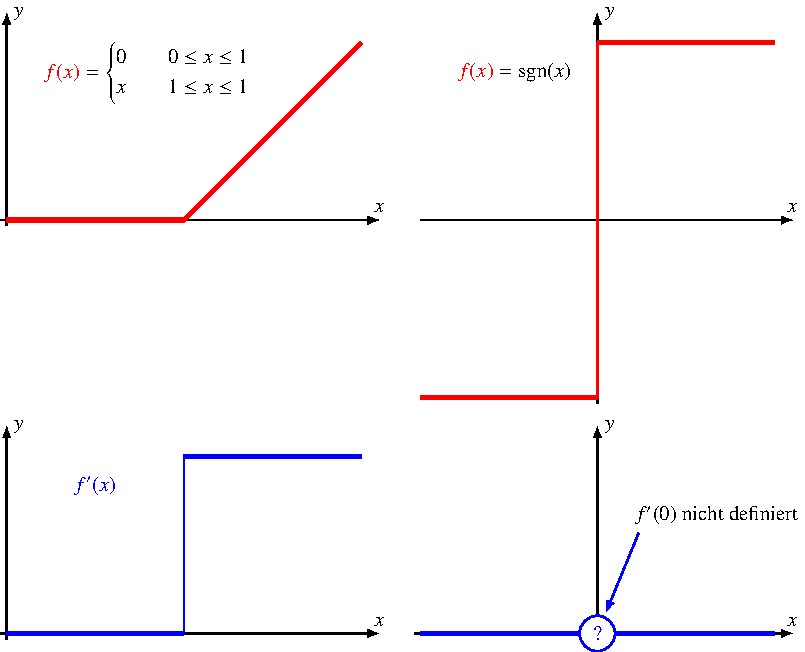
\includegraphics{chapters/010-skalarprodukt/images/schwach.pdf}
\caption{Schwache Ableitung einer nicht differenzierbaren Funktion.
Links die schwache Ableitung der Funktion von
Beispiel~\ref{buch:skalarprodukt:sobolevraum:bsp:schwachexistiert}.
Für die Signum-Funktion von
Beispiel~\ref{buch:skalarprodukt:sobolevraum:bsp:schwachexistiertnicht}
existiert die schwache Ableitung nicht, sie lässt für den Punkt $0$
nicht definieren.
\label{buch:skalarprodukt:sobolevraum:fig:schwach}}
\end{figure}
%
Die in Abbildung~\ref{buch:skalarprodukt:sobolevraum:fig:schwach} links
dargestellte Funktion
\[
f\colon (0,1) \to \mathbb{R}
:
x \mapsto
\begin{cases}
x&\qquad\text{für $0<x<1$}\\
1&\qquad\text{für $1\le x<2$}
\end{cases}
\]
ist stetig und integrierbar, aber sie ist an der Stelle $x=1$ nicht
differenzierbar.
Wir suchen die schwache Ableitung $v$ von $f$.

In einer Umgebung eines Punktes $x>1$ können wir Testfunktionen $\varphi$
so wählen, dass ihr Träger vollständig im Inneren des Intervals $(1,2)$
enthalten ist.
Mit diesen Testfunktionen können wir so rechnen, wie wenn $f$ die konstante
Funktion $1$ ist.
Das bedeutet für das Skalarprodukt
\[
\langle f,\varphi'\rangle
=
\int_1^2 \varphi'(x)\,dx
=
[\varphi(x)]_0^1 = 0.
\]
Das Skalarprodukt mit jeder beliebigen Testfunktion ist $0$, wir
müssen also $v(x)=0$ wählen.

Für $x$ im Teilinterval $(0,1)$ können wir die Testfunktionen so wählen,
dass der Träger vollständig im Inneren  von $(0,1)$ enthalten ist und
somit $f$ als die beliebig oft stetig differenzierbare Funktion $x$
behandelt werden darf.
Für das Skalarprodukt folgt dann
\[
-\langle f,\varphi'\rangle
=
-\int_0^1 f(x)\,\varphi'(x)\,dx
=
-\int_0^1 x\varphi'(x)\,dx
=
-[x\varphi(x)]_0^1 +\int_0^1 \varphi(x)\,dx
=
\langle 1,\varphi(x)\rangle,
\]
in diesem Teil des Intervals muss die schwache Ableitung den Wert $1$ 
haben.

Wir haben somit gefunden, dass die schwache Ableitung von $f$ die
Funktion
\[
v(x) = \begin{cases}
1&\qquad\text{für $0\le x<1$}
\\
0&\qquad\text{für $1< x<2$}
\end{cases}
\]
ist.
Wir kontrollieren dies, indem wir das Skalarprodukt für beliebige 
Testfunktionen $\varphi$ nachrechnen:
\begin{align*}
\langle v,\varphi\rangle
&=
\int_0^2 v(x)\,\varphi(x)\,dx
=
\int_0^1 1\,\varphi(x)\,dx
+
\int_1^2 0\,\varphi(x)\,dx.
\intertext{Jedes dieser Integrale kann man partiell integrieren:}
&=
[x\varphi(x)]_0^1 - \int_0^1 x\varphi'(x)\,dx
+
[1\varphi(x)]_1^2 - \int_1^2 1\varphi'(x)\,dx
\\
&=
\varphi(1) + \varphi(2) - \varphi(1) - \int_0^2 f(x)\,\varphi'(x)\,dx.
\intertext{Da $2$ ein Randpunkt ist, ist $\varphi(2)=0$, so dass sich}
&=-\langle f,\varphi'\rangle.
\end{align*}
ergibt.
Die Funktion $v$ ist also die schwache Ableitung von $f$.
\end{beispiel}

Eine Funktion in $W^{1,2}(\Omega)$ hat eine schwache Ableitung,
wie das Beispiel gezeigt hat, muss die Ableitung keine stetige
Funktion sein.
Ausserdem ist jede andere Funktion, die sich von der schwachen
Ableitung auf einer Menge vom Mass 0 unterscheidet, genauso eine
schwache Ableitung.
Trotzdem kann eine Funktion mit einer schwachen Ableitung nicht
beliebig ``wild'' sein, wie das folgende Beispiel zeigt.

\begin{beispiel}
\label{buch:skalarprodukt:sobolevraum:bsp:schwachexistiertnicht}
Die Signum-Funktion
\[
f\colon (-1,1) = \operatorname{sgn}(x) =
\begin{cases}
         - 1&\qquad\text{für $-1<x<0$}\\
\phantom{-}0&\qquad\text{für $x=0$}\\
\phantom{-}1&\qquad\text{für $0<x<1$}
\end{cases}
\]
ist nicht stetig (Abbildung~\ref{buch:skalarprodukt:sobolevraum:fig:schwach}).
$f$ ist fast überall konstant, in beiden Teilintervallen $(-1,0)$ und
$(0,1)$ ist die einzige mögliche schwache Ableitung von $f$ die
Nullfunktion.
Trotzdem kann $0$ nicht die schwache Ableitung von $f$ sein.
Wir wählen eine Testfunktion $\varphi$, die im Punkt $x=0$ von
Null verschieden ist.
Wäre $v$ eine schwache Ableitung von $f$, dann müsste
\begin{align*}
\langle v,\varphi\rangle
&=
-\langle f,\varphi'\rangle
=
-\int_{-1}^1 f(x) \varphi'(x)\,dx
\\
&=
-\int_{-1}^0 (-1)\cdot \varphi'(x)\,dx
-\int_{0}^1 1\cdot \varphi'(x)\,dx
=
\int_{-1}^0 \varphi'(x)\,dx
-
\int_{0}^1 \varphi'(x)\,dx
\\
&=
[\varphi(x)]_{-1}^0
-
[\varphi(x)]_{0}^1
=
\varphi(0)-\varphi(-1)
-
\varphi(1)+\varphi(0)
\\
&=
2\varphi(0)
\ne 0.
\end{align*}
Andererseits ist die Nullfunktion der einzige Kandidat für die
schwache Ableitun, für die das Skalarprodukt $\langle v,\varphi\rangle=0$
ist.
Dieser Widerspruch zeigt, dass die Funktion $f$ kein schwache
Ableitung hat.
\end{beispiel}

Die schwache Ableitung ermöglicht also mit gewissen Funktionen zu arbeiten,
die keine Ableitung im traditionellen Sinne haben.
Dank der Definition mit Hilfe eines Skalarproduktes in einem 
Hilbert-Raum darf man sich die Funktionen als Grenzwerte von
Cauchy-Folgen vorstellen.

%
% Physikalische Rechtfertigung
%
\subsection{Physikalische Rechtfertigung der schwachen Ableitung}
Die schwache Ableitung ersetzt die mit Hilfe eines Differenzenquotienten
definierte Änderungsrate durch eine Änderungsrate, die durch Vergleich
mit einer in der Umgebung eines Punktes konzentrierten Testfunktion
ermittelt wird.
Auf den ersten Blick mag das als Konzession an die Präzision der Ideen
der Analysis erscheinen, die Newton erfunden hat, um die Physik auf eine
neue Grundlage zu stellen.
Dabei wird aber vergessen, dass der Differenialquotient eine physikalisch
nicht erreichbare Idealisierung darstellt.
Keine Messung kann in einem Punkt im geometrischen Sinn erfolgen.
Die Bestimmung einer Position eines Massepunktes zum Beispiel erfolgt
durch Beobachtung des Lichtes, das vom Massepunkt reflektiert wird.
Doch der Massepunkt ist kein Punkt im geometrischen Sinn, er ist ausgedehnt
über ein endliches Gebiet.
Auch ist die Messung nicht instantan, es wird Licht gemessen, welches
über ein Zeitintervall vom Massepunkt reflektiert wird.
Das Messresultat entsteht also notwendigerweise als Mittelwert der
Beobachtung einer sehr grossen Zahl von Photonen, die von verschiedenen
Stellen reflektiert wurden.
Ein solcher Mittelwert ist genau das, was ein Skalarprodukt
$\langle f,\varphi\rangle$ mit einer Testfunktion ermittelt.

Die Feldgleichungen der Elektrodynamik wurden von Maxwell ausgehend
von Faradays Ideen als partielle Differentialgleichungen formuliert.
Sie verknüpfen die Werte des elektrischen Feldes $\vec{E}$ und des
magnetischen Feldes $\vec{B}$ mit der Ladungsdichte $\varrho$
und der Stromdichte $\vec{\jmath}$, die die Felder erzeugen.
Doch sowohl die Ladungsdichte wie auch die Stromdichte sind Idealisierungen.
Ladungen und Ströme sind nicht stetig über den Raum verteilt, sondern 
in Elektronen oder Atomkernen konzentriert.
Die Ladungsdichte entsteht daraus durch Messung der Ladung in einem kleine
Raumgebiet und Mittelung, was man wieder als Skalarprodukt mit einer
Testfunktion beschreiben kann.

Das elektrische Feld wird gemessen, indem die Kraft auf eine Testladung
im Feld ermittelt wird.
Ausser den prinzipiellen Einschränkungen an die Genauigkeit der
Positionsmessung wissen wir auch aus der Quantenmechanik, dass so etwas
wie die exakte Position eines Teilchens nicht gibt, wir können nur eine
Wahrscheinlichkeitsverteilung dafür bekommen.
Die Kraft äussert sich in einer Geschwindigkeitsänderung, die aber erst
messbar wird, wenn man die Beschleunigung eine gewisse Zeit lang aufrecht
erhält.
Das Messresultat ist also wieder ein Mittelwert über viele Positionen
und Zeitpunkte, oder anders ausgedrückt ein Skalarprodukt mit einer
Testfunktion.

Weitere Beispiele kann man auch in der Fluiddynamik finden.
Die Navier-Stokes-Gleichungen beschreiben die Strömung eines Mediums
unter der Annahme, dass es durch die Dichte $\varrho$ und die
Geschwindigkeit exakt beschreiben lässt.
Das Medium setzt sich aber aus einzelnen Atomen zusammen, die Dichte
ist also bereits ein Mittelwertbildung.
Bei der Geschwindigkeit wird das Problem noch deutlicher.
Auch die Strömungsgeschwindigkeit eines Gases ist der Mittelwert der
Strömungsgeschwindigkeit der Teilchen. 
Die Geschwindigkeit einzelner Teilchen ist dabei meistens sehr viel
grösser, nämlich im Bereich der Schallgeschwindigkeit, und äussert sich
in der Temperatur des Gases, also der mittleren kinetischen Energie.
Es ist nicht sinnvoll, von der Temperatur eines einzelnen Atoms zu
sprechen.

Alle diese Beispiele zeigen, dass die Ableitung als Änderungsrate, die
mit einem Differenzenquotienten bestimmt werden kann, eine Idealisierung
ist.
Wir können dies sogar etwas formeller zeigen.
Sei $x(t)$ die Koordinate eines Massepunktes zur Zeit $t$.
Die Messung kann nicht instantan erfolgen, im besten Fall ist die
gemessene Position ein Integral der Form
\[
\hat{x}(t)
=
\int_{-\infty}^\infty x(\tau) \varphi(\tau - t)\,d\tau.
\]
Darin ist $\varphi$ eine Testfunktion mit Träger in der Nähe von $0$.
Schreiben wir $T_t\varphi(\tau) = \varphi(\tau -t)$, dann können wir
das Messresultat auch als Skalarprodukt
$\hat{x}(t)=\langle x,T_t\varphi\rangle$
schreiben.
Die Messung mit der gleichen Aparatur einen Moment $\Delta t$ später ergibt
\[
\hat{x}(t+\Delta t)
=
\int_{-\infty}^\infty x(\tau) \varphi(\tau-t-\Delta t)\,dt
=
\langle x, T_{t+\Delta t}\varphi\rangle.
\]
Die Geschwindigkeit als Differenzenquotient ist
\begin{equation}
\frac{
\hat{x}(t+\Delta t)-\hat{x}(t)
}{\Delta t}
=
\frac{
\langle f,T_{t+\Delta t}\varphi\rangle
-
\langle f,T_{t}\varphi\rangle
}{
\Delta t
}
=
\left\langle
f,\frac{T_{t+\Delta t}\varphi - \varphi}{\Delta t}
\right\rangle
\label{buch:skalarprodukt:sobolevlraum:eqn:geschwindigkeit}
\end{equation}
Die Funktion $(T_{t+\Delta t}\varphi-T_t\varphi)/\Delta t$ ist eine 
beliebig oft stetig differenzierbare Funktion, die im Grenzwert
$\Delta t\to 0$ gegen
\[
\frac{
\varphi(\tau - t - \Delta t)
-
\varphi(\tau - t)
}{
\Delta t
}
=
-
\frac{
\varphi(\tau - t + \delta) - \varphi(\tau - t)
}{
\delta
}
\to 
-
\varphi'(\tau - t)
\quad
\text{für $\delta = - \Delta \to 0$}
\]
konvergiert.
Der Differenzenquotient
\eqref{buch:skalarprodukt:sobolevlraum:eqn:geschwindigkeit}
konvergiert daher gegen
\[
\lim_{\Delta t\to 0}
\frac{
\hat{x}(t+\Delta t)-\hat{x}(t)
}{\Delta t}
=
\left\langle
x,
\lim_{\Delta t\to 0}
\frac{T_{t+\Delta t}\varphi-T_t\varphi}{\Delta t}
\right\rangle
=
\langle f,-\varphi'\rangle
=
-
\langle f, \varphi'\rangle.
\]
Dieses einfache Modell einer ``unscharfen'' Messung führt also automatisch
auf das Konzept der schwachen Ableitung.








%\uebungsabschnitt
%\aufgabetoplevel{chapters/010-potenzen/uebungsaufgaben}
%\begin{uebungsaufgaben}
%\uebungsaufgabe{101}
%\uebungsaufgabe{102}
%\uebungsaufgabe{103}
%\uebungsaufgabe{104}
%\end{uebungsaufgaben}
%\endgroup


%
% chapter.tex -- Skalarprodukt
%
% (c) 2021 Prof Dr Andreas Müller, Hochschule Rapperswil
%
% !TeX spellcheck = de_CH
\chapter{Skalarprodukte
\label{buch:chapter:skalarprodukte}}
\kopflinks{Skalarprodukte}

%
% 1-definition.tex
%
% (c) 2023 Prof Dr Andreas Müller, OST Ostschweizer Fachhochschule
%
\section{Definition
\label{buch:opertoren:section:definition}}
\kopfrechts{Definition}


%
% 2-cauchyschwarz.tex
%
% (c) 2022 Prof Dr Andreas Müller, OST Ostschweizer Fachhochschule
%
\section{Ungleichungen
\label{buch:skalarprodukte:section:cauchyschwarz}}
\kopfrechts{Cauchy-Schwarz-Ungleichung}
In der Vektorgeometrie wird gelehrt, dass die Länge eines Vektors $u$
durch die Norm $\|u\|$ wiedergegeben wird und dass die geometrische
Intuition dazu passt.
Dazu gehört vor allem, dass die Dreiecksungleichung erfüllt ist,
dass also für drei Punkt $A$, $B$ und $C$
\begin{equation}
\overline{AB} \le \overline{AC} + \overline{BC}
\label{skalarprodukt:ungleichungen:eqn:dreieck}
\end{equation}
gilt.
In Vektorform bedeutet dies, dass
\[
\| b-a\|
\le
\| c-a\| + \|b-c\|.
\]
Schreibt man $u=c-a$ und $v=b-c$, dann ist $u+v=b-a$ und somit
\begin{equation}
\| u+v\| \le \|u\| + \|v\|.
\label{skalarprodukt:cauchyschwarz:eqn:dreieck0}
\end{equation}
Dies ist die Dreiecksungleichung in
Vektorform~\eqref{skalarprodukt:cauchyschwarz:eqn:dreieck0}.
Ziel dieses Abschnitts ist zu zeigen, dass jedes reelle oder
komplexe Skalarprodukt diese und weitere Eigenschaften automatisch
mitbringt.

%
% Cauchy-Schwarz-Ungleichung
%
\subsection{Cauchy-Schwarz-Ungleichung}
Sei also $\langle\;\,,\;\rangle$ ein reelles oder komplexes Skalarprodukt
auf dem Vektorraum $V$,
insbesondere ist $\langle v,v\rangle\ge 0$ für beliebige Vektoren $v\in V$.
Für zwei Vektoren $x,y\in V$ und $t\in \mathbb{R}$  gilt daher
\begin{align}
0
&\le
\| x+ty\|^2
=
\langle x+ty,x+ty\rangle
=
\langle x,x\rangle
+
t\langle x,y\rangle
+
t\langle y,x\rangle
+
t^2
\langle y,y\rangle.
\label{skalarprodukt:cauchyschwarz:eqn:quadrat}
\end{align}
Für ein reelles Skalarprodukt ist $\langle x,y\rangle=\langle y,x\rangle$
und damit
\begin{align}
0
&\le
\|x\|^2 + 2t\langle x,y\rangle + t^2 \|y\|^2.
\label{buch:skalarprodukt:cauchyschwarz:eqn:cspoly}
\end{align}
Dies ist ein quadratisches Polynom in der Variablen $t$, dessen Minimum
nicht negativ sein darf.

%
% Minimum eines quadratischen Polynoms
%
\subsubsection{Minimum eines quadratischen Polyoms}
Ein beliebiges quadratisches Polynom
\[
p(t)=at^2+bt+c
\]
kann durch
quadratisches Ergänzen in die Form
\[
p(t)
=
a\biggl(t+\frac{b}{2a}\biggr)^2 -\frac{b^2}{4a}+c
\]
gebracht werden.
Daraus kann man ablesen, dass das Minimum an der Stelle
\[
t_0
=
-\frac{b}{2a}
\]
angenommen wird und den Wert 
\begin{equation}
p(t_0)
=
c-\frac{b^2}{4a}
\end{equation}
hat.
Die gleiche Lösung kann natürlich auch durch Bestimmung des Minimums
von $p(t)$ mit Hilfe der Bedingung $p'(t_0)=0$ gefunden werden.

%
% Cauchy-Schwarz-Ungleichung für einen reellen Vektorraum
%
\subsubsection{Cauchy-Schwarz-Ungleichung für einen reellen Vektorraum}
Für~\eqref{buch:skalarprodukt:cauchyschwarz:eqn:cspoly}
ist
\[
a=\|y\|^2,\quad
b=2\langle x,y\rangle
\quad\text{und}\quad
c=\|x\|^2.
\]
Daher folgt aus~\eqref{buch:skalarprodukt:cauchyschwarz:eqn:cspoly}
\[
0
\le
\|x\|^2 - \frac{\langle x,y\rangle^2}{\|y\|^2}
\qquad\Rightarrow\qquad
\langle x,y\rangle^2 \le \|x\|^2\, \|y\|^2
\qquad\Rightarrow\qquad
|\langle x,y\rangle| \le \|x\|\, \|y\|.
\]
Dies ist die Cauchy-Schwarz-Ungleichung für das Skalarprodukt
$\langle \;\,,\;\rangle$.

\begin{satz}[Cauchy-Schwarz]
\label{buch:skalarprodukt:cauchy-schwarz:satz:reell}
Ein reelles Skalarprodukt $\langle\;\,,\;\rangle$ auf dem reellen Vektorraum
$V$ erfüllt die Cauchy-Schwarz-Ungleichung
\[
|\langle x, y\rangle| \le \|x\|\,\|y\|
\]
für $x,y\in V$.
\end{satz}

%
% Cauchy-Schwarz-Ungleichung für einen komplexen Vektorraum
%
\subsubsection{Cauchy-Schwarz-Ungleichung für einen komplexen Vektorraum}
Für ein komplexes Skalarprodukt ist das Produkt $\langle x,y\rangle$
nicht mehr unbedingt reell und kann damit nicht mehr direkt mit den
Normen $\|x\|^2u$ und $\|y\|^2$ vergleichen.
Wir ersetzen daher $t$ durch
$t\langle y,x\rangle=t\overline{\langle x,y\rangle}$
und erhalten 
\begin{align*}
0
\le
\|x+t\langle y,x\rangle y\|^2
&=
\langle x,x\rangle
+t\langle y,x\rangle \langle x,y\rangle
+t\overline{\langle y,x\rangle}\langle y,x\rangle
+t^2\langle y,y\rangle
\\
&=
\|x\|^2
+
t
2|\langle x,y\rangle|^2
+
t^2 |\langle x,y\rangle|^2
\|y\|^2.
\end{align*}
Dies ist wieder ein quadratisches Polynom, diesmal mit den Koeffizienten
\[
a= |\langle x,y\rangle|^2 \|y\|^2,
\quad
b= 2|\langle x,y\rangle|^2
\quad\text{und}\quad
c= \|x\|^2.
\]
Das Minimum dieses Polynoms ist nach
\[
0
\le
c-\frac{b^2}{4a}
=
\|x\|^2 - \frac{|\langle x,y\rangle|^4}{|\langle x,y\rangle|^2\,\|y\|^2}
=
\|x\|^2 - \frac{|\langle x,y\rangle|^2}{\|y\|^2}
\quad\Rightarrow\quad
|\langle x,y\rangle|^2 \le \|x\|^2\,\|y\|^2
\quad\Rightarrow\quad
|\langle x,y\rangle \le \|x\|\,\|y\|.
\]
Dies ist die Cauchy-Schwarz-Ungleichung für einen komplexen Vektorraum.

\begin{satz}[Cauchy-Satz]
\label{buch:skalarprodukt:cauchy-schwarz:satz:komplex}
Ein komplexes Skalarprodukt $\langle\;\,,\;\rangle$ auf dem komplexen Vektorraum
$V$ erfüllt die Cauchy-Schwarz-Ungleichung
\[
|\langle x, y\rangle| \le \|x\|\,\|y\|
\]
für $x,y\in V$.
\end{satz}

Man beachte, dass die
Sätze~\ref{buch:skalarprodukt:cauchy-schwarz:satz:reell}
und
\ref{buch:skalarprodukt:cauchy-schwarz:satz:komplex}
nur die Axiome eines Skalarproduktes verwenden.
Sie gelten also
ganz unabhängig von der konkreten Definition des Skalarproduktes,
solange die Eigenschaften eines Skalarproduktes gegeben sind.

\begin{beispiel}
Die sesquilineare Funktion
\[
\langle x,y\rangle
=
\sum_{i=1}^n\overline{x}_i y_i
\]
für Vektoren $x,y\in\mathbb{C}^n$ ist positiv definit, denn
\[
\langle x,x\rangle
=
\sum_{i=1}^n \overline{x}_i x_i = \sum_{i=1}^n |x_i|^2 > 0
\]
für $x\ne 0$.
Nach Satz~\ref{buch:skalarprodukt:cauchy-schwarz:satz:komplex}
gilt daher
\[
\biggl|
\sum_{i=1}^n \overline{x}_i y_i
\biggr|
\le
\sqrt{\sum_{i=1}^n |x_i|^2} \sqrt{\sum_{i=1}^n |y_i|^2}
\quad\text{oder auch}\quad
\biggl|
\sum_{i=1}^n x_i y_i
\biggr|
\le
\sqrt{\sum_{i=1}^n |x_i|^2} \sqrt{\sum_{i=1}^n |y_i|^2}
\]
für beliebige Vektoren $x,y\in\mathbb{C}^n$.
\end{beispiel}

\begin{beispiel}
Die sesquilineare Funktion
\[
\langle f,g\rangle
=
\int_a^b \overline{f(x)} g(x)\,dx
\]
für komplexwertige, stetige Funktion auf dem Intervall $[a,b]$
ist positiv definit, denn
\[
\langle f,f\rangle
=
\int_a^b \overline{f(x)} f(x)\,dx
=
\int_a^b |f(x)|^2\,dx
\ge 0
\]
für $f\ne 0$.
Nach Satz~\ref{buch:skalarprodukt:cauchy-schwarz:satz:komplex}
gilt daher
\begin{align*}
\biggl|\int_a^b \overline{f(x)}g(x)\,dx\biggr|
&\le
\sqrt{\int_a^b |f(x)|^2\,dx}
\sqrt{\int_a^b |g(x)|^2\,dx}
\intertext{oder auch}
\biggl|\int_a^b f(x) g(x)\,dx\biggr|
&\le
\sqrt{\int_a^b |f(x)|^2\,dx}
\sqrt{\int_a^b |g(x)|^2\,dx}
\end{align*}
für beliebige komplexwertige stetige Funktionen $f,g$ auf dem
Intervall $[a,b]$.
\end{beispiel}

%
% Dreiecksungleichung
%
\subsection{Dreiecksungleichung}
Die Intuition einer Längenmessung basiert auf der
Dreiecksungleichung~\eqref{skalarprodukt:ungleichungen:eqn:dreieck}.
Sie ist gleichbedeutend mit der
Vektorform~\eqref{skalarprodukt:cauchyschwarz:eqn:dreieck0}
der Ungleichung.

Die Cauchy-Schwarz-Ungleichung ermöglicht nun, diese Ungleichung
nachzurechnen.
Die Norm von $\|x+y\|^2$ ist
\[
\|x+y\|^2
=
\langle x+y,x+y\rangle
=
\langle x,x\rangle
+
\langle x,y\rangle
+
\langle y,x\rangle
+
\langle y,y\rangle
=
\|x\|^2 + 2\operatorname{Re}\langle x,y\rangle + \|y\|^2.
\]
Den mittleren Term kann man mit der Cauchy-Schwarz-Ungleichung
umformen:
\begin{align*}
\|x\|^2 + 2\operatorname{Re}\langle x,y\rangle + \|y\|^2.
&\le
\|x\|^2 + 2|\operatorname{Re}\langle x,y\rangle| + \|y\|^2.
\\
&\le
\|x\|^2 + 2|\langle x,y\rangle| + \|y\|^2.
\\
&\le
\|x\|^2 + 2\|x\|\,\|y\| + \|y\|^2
=
(\|x\| + \|y\|)^2.
\end{align*}
Durch Ziehen der Wurzel folgt
\[
\|x+y\| \le \|x\| + \|y\|.
\]
Damit ist der folgende Satz bewiesen.

\begin{satz}[Dreiecksungleichung]
Für die Norm zu einem beliebigen Skalarprodukt auf dem reellen
oder komplexen Vektorraum $V$ gilt die Dreiecksungleichung
\[
\|x+y\| \le \|x\| + \|y\|
\]
für $x,y\in V$.
\end{satz}

%
% Normen
%
\subsection{Normen
\label{skalarprodukt:cauchyschwarz:subsection:norm}}
Das Skalarprodukt ist nicht die einzige Möglichkeit, eine Norm auf
einem Vektorraum zu definieren.
Zum Beispiel kann man auf $\mathbb{C}^n$ die sogenannte $l^1$-Norm
definieren.

\begin{definition}
Die Funktion
\[
\|x\|_1
=
\sum_{i=1}^n |x_i|
\]
für $x\in\mathbb{C}^n$ heisst die {\em $l^1$-Norm} auf $\mathbb{C}^n$.
\end{definition}

Die Funktion $\|\cdot\|_1$ ist eine Norm im Sinne der folgenden Definition.

\begin{definition}
Eine Funktion $\|\cdot\| \colon V\to\mathbb{R}$ auf einem reellen
oder komplexen Vektorraum $V$ heisst eine {\em Norm}, wenn Sie die
folgenden Bedingungen erfüllt
\begin{enumerate}
\item
$\|\lambda x\| = |\lambda|\, \|x\|$ für $x\in V$ und $\lambda\in \Bbbk$
\item
Für alle Vektoren $x\in V$ mit $x\ne 0$ gilt $\|x\|>0$.
\item
Dreiecksungleichung: $\|x+y\| \le \|x\| + \|y\|$ für alle $x,y\in V$
\end{enumerate}
\end{definition}

Es ist klar, dass die $l^1$-Norm die Bedingungen~1 und 2 erfüllt.
Aber auch die Bedingung~3 kann man leicht  nachprüfen:
\[
\|x+y\|_1
=
\sum_{i=1}^n |(x+y)_i|
=
\sum_{i=1}^n |x_i+y_i|
\le
\sum_{i=1}^n(|x_i|+|y_i|)
=
\sum_{i=1}^n|x_i|
+
\sum_{i=1}^n|y_i|
=
\|x\|_1 + \|y\|_1,
\]
wozu wir nur die Dreiecksungleichung $|a+b|\le |a| + |b|$ für reelle 
oder komplexe Zahlen $a,b$ benötigen.

\begin{beispiel}
Die Funktion
\[
\|x\|_\infty = \sup_{1\le i\le n} |x_i|
\]
ist eine Norm auf $\mathbb{C}^n$.
\end{beispiel}

Auch in diesem Fall sind die Bedingungen~1 und 2 ganz offensichtlich erfüllt.
Für die Dreiecksungleichung rechnen
\begin{align*}
\|x+y\|_\infty
&=
\sup_{1\le i\le n} |x_i+y_i|
\le
\sup_{1\le i\le n} (|x_i|+|y_i|)
\le
\sup_{1\le i\le n} |x_i|+\sup_{1\le i\le n}|y_i|
=
\|x\|_\infty + \|y\|_\infty.
\end{align*}
Somit ist $\|\cdot\|_\infty$ eine Norm auf $\mathbb{C}^n$.

%
% Polaridentität
%
\subsection{Polaridentität}
Die durch das Skalarprodukt definierte Norm
\( \|x\|^2=\langle x,x\rangle \)
ist nach Abschnitt~\ref{skalarprodukt:cauchyschwarz:subsection:norm}
ein Spezialfall einer Norm.
Ist es möglich, für eine Norm, die von einem Skalarprodukt herkommt,
das Skalarprodukt wieder zu rekonstruieren?

%
% Reelles Skalarprodukt aus der Norm
%
\subsubsection{Reelles Skalarprodukt aus der Norm}
Die Antwort gibt der folgende Satz.

\begin{satz}[Polaridentität]
\label{skalarprodukt:cauchyschwarz:satz:polarformel}
Ist $\|\cdot\|$ die Norm zu einem Skalarprodukt auf dem reellen Vektorraum
$V$, dann kann das Skalarprodukt zweier Vektoren $x,y\in V$ mittels
der sogenannten {\em Polaridentität}
\index{Polaridentität}%
\begin{equation}
\langle x, y\rangle
=
\frac12\bigl(
\|x+y\|^2 - \|x\|^2 - \|y\|^2 
\bigr)
\label{skalarprodukt:cauchyschwarz:eqn:polar}
\end{equation}
berechnet werden.
\end{satz}

\begin{proof}[Beweis]
Die Gleichung
\begin{align*}
\|x+y\|^2
&=
\langle x+y,x+y\rangle
=
\|x\|^2 + 2\langle x,y\rangle + \|y\|^2 
\end{align*}
kann nach $\langle x,y\rangle$ aufgelöst werden und ergibt
die behauptete Formel~\eqref{skalarprodukt:cauchyschwarz:eqn:polar}.
\end{proof}

% 
% Parallelogrammgleichung
%
\subsubsection{Parallelogrammgleichung}
\begin{figure}
\centering
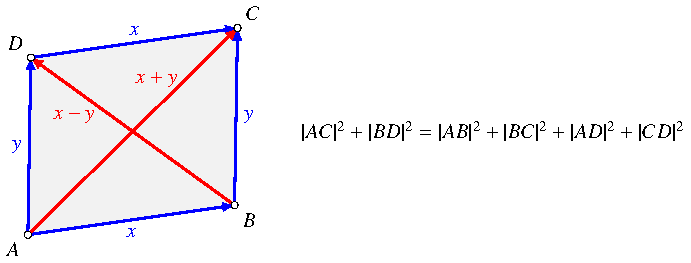
\includegraphics{chapters/010-skalarprodukt/images/parallelogramm.pdf}
\caption{Parallelogrammregel für eine Norm, die aus einem Skalarprodukt
entsteht.
\label{skalarprodukt:cauchyschwarz:fig:parallelogramm}}
\end{figure}
Die Polaridentitäten können auch noch in einer anderen Form geschrieben
werden.
Dazu berechnet man zusätzlich die Norm von $x-y$:
\begin{align*}
\|x+y\|^2
&=
\|x\|^2 + \|y\|^2 + 2\langle x, y\rangle
\\
\|x-y\|^2
&=
\|x\|^2 + \|y\|^2 - 2\langle x, y\rangle
\\
\|x+y\|^2 +\|x-y\|^2
&=
2\|x\|^2 + 2\|y\|^2
\end{align*}

\begin{satz}
\label{skalarprodukt:cauchyschwarz:satz:parallelgramm}
Für eine Norm, die von einem reellen Skalarprodukt herkommt, gilt die
Parallelogrammformel
\begin{equation}
\|x+y\|^2 +\|x-y\|^2
=
2\|x\|^2 + 2\|y\|^2.
\label{skalarprodukt:cauchyschwarz:eqn:parallelgramm}
\end{equation}
(Abbildung~\ref{skalarprodukt:cauchyschwarz:fig:parallelogramm})
\end{satz}

Das Skalarprodukt kann man damit auf verschiedene Weise aus der
Norm gewinnen:
\begin{equation}
\begin{aligned}
\langle x, y\rangle
&=
{\textstyle\frac12}\bigl( \|x\|^2 + \|y\|^2 - \|x+y\|^2 \bigr)
\\
&=
{\textstyle\frac12}\bigl(
\|x+y\|^2
-
\|x\|^2 
-
\|y\|^2
\bigr)
\\
&=
{\textstyle\frac14}\bigl(
\|x+y\|^2 - \|x-y\|^2
\bigr).
\end{aligned}
\label{skalarprodukt:cauchyschwarz:eqn:realteil}
\end{equation}
Nur die letzte Formel ist noch nicht gut begründet.
Man kann aber sofort nachrechnen, dass 
\begin{align*}
\|x+y\|^2&=\|x\|^2+2\langle x,y\rangle+\|y\|^2\\
\|x-y\|^2&=\|x\|^2-2\langle x,y\rangle+\|y\|^2
\intertext{die Differenz}
\|x+y\|^2 - \|x-y\|^2 &= 4\langle x,y\rangle
\qquad
\Rightarrow
\qquad
\langle x,y\rangle
=
\frac14\bigl(\|x+y\|^2 - \|x-y\|^2\bigr)
\end{align*}
haben.

%
% Komplexes Parallelogramm aus der Norm
%
\subsubsection{Komplexe Skalarprodukt}
Das Resultat von Satz~\ref{skalarprodukt:cauchyschwarz:satz:polarformel}
gilt in abgeänderter Form auch für komplexe Skalarprodukte.
Da das Skalarprodukt auch einen nichtverschwindenen Imaginärteil haben
kann, wird eine zusätzliche Gleichung zur Berechnung des Imaginärteils
nötig.
Eine solche kann gewonnen werden, indem zusätzlich die Normen
$\|x+iy\|^2$ und $\|x-iy\|^2$ berechnet werden.
Dazu ist zu beachten, dass
\[
\langle x,y\rangle
-
\langle y,x\rangle
=
\langle x,y\rangle
-
\overline{
\langle x,y\rangle
}
=
2i\operatorname{Im}\langle x,y\rangle
\]
Damit erhält man
\begin{align*}
\|x+iy\|^2 &= \|x\|^2 + i\langle x,y\rangle - i\langle y,x\rangle + \|y\|^2 
           = \|x\|^2 + 2\operatorname{Im}\langle x,y\rangle + \|y\|^2 \\
\|x-iy\|^2 &= \|x\|^2 - i\langle x,y\rangle + i\langle y,x\rangle + \|y\|^2 
           = \|x\|^2 - 2\operatorname{Im}\langle x,y\rangle + \|y\|^2.
\end{align*}
Damit kann man nach dem Imaginärteil des Skalarproduktes auflösen und
die Formeln
finden, die den Formeln
\eqref{skalarprodukt:cauchyschwarz:eqn:realteil}
für das reelle Skalarprodukt entsprechen.
\eqref{skalarprodukt:cauchyschwarz:eqn:realteil}
Formeln bleiben gültig als Formeln für den Realteil des Skalarproduktes.
Damit haben wir den folgenden Satz gefunden.

\begin{satz}[Polaridentitäten für ein komplexes Skalarprodukt]
Ist $\|\cdot\|$ die Norm, die aus dem komplexen Skalarprodukt
$\langle\;\,,\;\rangle$ auf einem Vektorraum $V$ gewonnen wurde,
dann können Real- und Imaginärteil mit den Formeln
\begin{align*}
\operatorname{Re}\langle x,y\rangle
&=
{\textstyle\frac12}\bigl(
\|x+y\|^2 - \|x\|^2 -\|y\|^2
\bigr)
\\
&=
{\textstyle\frac12}\bigl(
\|x\|^2 +\|y\|^2 - \|x+y\|^2
\bigr)
\\
&=
{\textstyle\frac14}\bigl(
\|x+y\|^2 - \|x-y\|^2
\bigr),
\\
\operatorname{Im}\langle x,y\rangle
&=
{\textstyle\frac12}\bigl(
\|x+iy\|^2-\|x\|^2-\|y\|^2
\bigr)
\\
&=
{\textstyle\frac12}\bigl(
\|x\|^2+\|y\|^2-\|x-iy\|^2
\bigr)
\\
&=
{\textstyle\frac14}\bigl(
\|x+iy\|^2
-
\|x-iy\|^2
\bigr)
\end{align*}
für beliebige Vektoren $x,y\in V$
allein aus Werten der Norm berechnet werden.
\end{satz}


%
% 3-funktionenraeume.tex
%
% (c) 2022 Prof Dr Andreas Müller, OST Ostschweizer Fachhochschule
%
\section{Funktionenräume
\label{buch:skalarprodukt:section:funktionenraeume}}
\kopfrechts{Funktionenräume}
Ziel der harmonischen Analysis ist die effiziente Approximation einer
grossen Klasse von Funktionen.
Als approximierende Funktionen kommen stetige Funktionen, Polynome,
trigonometrische Polynome oder eine ähnlich, einfach konstruierbare
Funktionenfamilie in Frage.
Es gilt zunächst herauszufinden, was ``Approximation'' genau heissen
soll und von welchen Funktionen man überhaupt erwarten kann, dass sie
approximiert werden können.

%
% Stetige Funktionen
%
\subsection{Stetige Funktionen
\label{buch:skalarprodukt:subsection:stetige-funktionen}}
Der frühe intuitive Funktionsbegriff ging oft von der Vorstellung einer
in einem Strich gezeichneten Kurve aus, wie man sie von den Graphen
der Polynome oder der trigonometrischen Funktionen her kennt.
In moderner Sprechweise sind dies die stetigen Funktionen.

\begin{definition}
Eine Funktion $f\colon I\to\mathbb{R}$ mit $I\subset \mathbb{R}$
heisst stetig in einem Punkt $x_0\in I$, wenn für jedes $\varepsilon>0$
ein $\delta>0$ existiert derart, dass $f(x)-f(x_0)|<\delta$ sobald
$|x-x_0|<\varepsilon$.
\end{definition}

Nur die Eigenschaft, eine Abstandsmessung zu besitzen, wird vom
Definitionsbereich $I\subset \mathbb{R}$ verlangt.
Der Stetigkeitsbegriff kann daher verallgemeinert werden auf den
Begriff des metrischen Raumes.

\begin{definition}
Eine {\em Metrik} auf einer Menge $X$ ist eine Funktion
\index{Metrik}%
$d\colon X\times X\to \mathbb{R}$
mit den folgenden Eigenschaften
\begin{enumerate}
\item
Positiv definit: $d(x,y)\ge 0$ und $d(x,y)$ genau dann, wenn $x=y$.
\item
Symmetrie: \(d(x,y)=d(y,x)\)
\item
Dreiecksungleichung: \( d(x,y) \le d(x,z) + d(z,y) \).
\end{enumerate}
Ein {\em metrischer Raum} ist ein Menge $X$ mit einer Metrik.
\index{matrischer Raum}%
\end{definition}

In einem metrischen Raum ist der Begriff des Grenzwertes übertragbar.
Mit dem Begriff des Grenzwertes lässt sich auch der Begriff der
Stetigkeit verallgemeinern.

\begin{definition}
Ist $x_n\in X$ eine Folge von Punkten in einem metrischen Raum $X$,
dann heisst $x$ der Grenzwert der Folge $x_n$, wenn es für jedes
$\varepsilon>0$ ein $N>0$ gibt derhart, dass
$d(x_n,x)\le \varepsilon$ für alle $n>N$.
Eine Funktion $f\colon X\to Y$ zwischen metrischen Räumen heisst
stetig im Punkt $x\in X$, wenn für jede Folge $x_n\in X$ mit
Grenzwert $x$ auch die Folge $y_n=f(x_n)\in Y$ konvergiert und
den Grenzwert $y=f(x)$ hat.
\end{definition}

Teilmengen von $\mathbb{R}$ oder $\mathbb{R}^n$ tragen natürlich
die Struktur eines metrischen Raumes mit der Abstandsmessung in 
$\mathbb{R}^n$ als Metrik
\[
d(x,y) = \sqrt{(x_1-y_1)^2 + \ldots + (x_n-y_n)^2} = \|x-y\|.
\]
Die Eigenschaften einer Metrik wurden bereits in Abschnitt
\ref{buch:skalarprodukte:section:cauchyschwarz} nachgewiesen.

Der Begriff des Grenzwertes klärt, was mit der Approximation von $x$
durch eine Folge $x_n$ gemeint ist.
Wenn man darauf aufbauend die Konvergenz einer Folge von Funktionen
gegen eine Grenzfunktion definieren will, braucht man einen Abstansbegriff
zwischen Funktionen.
Ein erster Versuch könnte sein, als Abstand zwischen zwei Funktionen
$f$ und $g$ die Funktion
\[
d(f,g) = |f(x_0) - g(x_0)|.
\]
Die Menge der Funktionen wird dadurch jedoch nicht zu einem metrischen
Raum.
Zwar gilt sicher die Symmetrie und Dreiecksungleichung, und auch 
$d(f,g)\ge 0$ für beliebige Funktionen.
Aber wenn $d(f,g)=0$ ist, heisst das nur, dass $f$ und $g$ im Punkt
$x_0$ den gleichen Wert haben.
Ausser in trivialen Fällen wird es Funktionen geben, die zwar im Punkt
$x_0$ übereinstimmen, sich aber in mindestens einem anderen Punkt
unterscheiden.

%
% Normierte Räume
%
\subsubsection{Normierte Räume}
Die stetigen Funktionen bilden aber keine strukturlose Menge, sie
bilden einen Vektorraum: die Summe von stetigen Funktionen ist ebenfalls
stetig, multiplizieren einer stetigen Funktion mit einem Skalar führt
nicht aus der Menge der stetigen Funktionen heraus.
Die für den Grenzwertbegriff von Funktionen verwendete Abstandsmessung 
sollte der Vektorraumstruktur ebenfalls Rechnung tragen.

\begin{definition}
\label{buch:skalaprodukt:funktionenraume:def:norm}
Sei $V$ ein Vektorraum über $\mathbb{R}$, dann heisst eine Funktion
\( \|\;\cdot\;\| \colon V \to \mathbb{R}\) eine {\em Norm}, wenn gilt
\index{Norm}
\begin{enumerate}
\item
Definit: $ \|x\| = 0 \Rightarrow x=0$
\item
Homogeneität: $ \| \lambda x \| = |\lambda| \cdot \|x\|$
\item
Dreiecksungleichung: $\|x+y\| \le \|x\| + \|y\|$
\end{enumerate}
Ein {\em normierter Raum} ist ein Vektorraum $V$ mit einer Norm.
\end{definition}

%
% Vollständigkeit
%
\subsubsection{Vollständigkeit}
In den rationalen Zahlen hat nicht jede Folge einen Grenzwert.
Die Zahl $\sqrt{2}$ lässt sich beliebig genau durch rationale Zahlen
approximieren, sie ist aber nicht in $\mathbb{Q}$.
Ähnlich lässt sich die Funktion $x\mapsto \sqrt{x}$ beliebig genau 
durch Polyome approximieren, sie ist aber selbst kein Poylnome

\begin{definition}
Ein Folge $x_n\in X$ in einem metrischen Raum heisst {\em Cauchy-Folge},
wenn es für jedes $\varepsilon>0$ ein $N>0$ gibt derart, dass 
$|x_n-x_m|<\varepsilon$ wenn $n,m>N$ ist.
\end{definition}

Cauchy-Folgen sind also Folgen, die sich für genügend grossen Index
kaum mehr ändern und für die man daher Konvergenz erwarten würde.

\begin{definition}
Ein normierter Raum heisst {\em vollständig} oder ein Banach-Raum,
wenn jede Cauchy-Folge einen Grenzwert hat.
\end{definition}

Die rationalen Zahlen $\mathbb{Q}$ bilden keinen vollständigen
metrischen Raum, aber die reellen Zahlen $\mathbb{R}$ enthalten
alle Grenzwerte von Cauchy-Folgen, $\mathbb{R}$ ist eine vollständiger
metrischer Raum.
Die Menge der Polynome, betrachtet als Teilmenge der Menge der
stetigen Funktionen $[0,1]\to\mathbb{R}$ ist nicht vollständig,
da es eine Folge $f_n(x)$ von Approximationsfunktionen der Funktion
$x\mapsto \sqrt{x}$ gibt.
Als Cauchy-Folge konvergiert sie zwar gegen eine stetige Funktion,
aber die Grenzfunktion ist nicht mehr im Raum der Polynome.

Das Ziel der folgenden Kapitel ist also, zu geeignet interessanten
Funktionenfamilien ``gute'' Normen zu finden derart, dass Cauchy-Folgen
konvergieren gegen Funktionen, die immer noch ausreichend viele
nützliche Eigenschaften haben.
Im besten Fall konvergieren stetige Funktionen gegen stetige Funktionen,
es wird sich aber zeigen, dass diese Anforderung zu streng ist.

%
% Norm fpr stetige Funktionen
%
\subsection{Norm für stetige Funktionen
\label{buch:skalarprodukt:subsection:normfuerstetigefunktionen}}
Damit man von Konvergenz von Folgen stetiger Funktionen sprechen kann,
brauchen wir jetzt also eine Norm für stetige Funktionen.

\begin{definition}
Sei $X$ ein metrischer Raum und
\[
C(X)
=
C_{\mathbb{R}}(X)
=
\{
f\colon X \to\mathbb{R}\mid
\text{$f$ ist stetig}
\}
\]
der Vektorraum der stetigen Funktion auf $X$.
Die Norm von $C(X)$ ist definiert als
\[
\|f\| = \sup_{x\in X} |f(x)|.
\]
Sie heisst die {\em Supremum-Norm}.
\end{definition}

Wir prüfen nach, dass die Supremum-Norm tatsächlich eine Norm ist.
Dazu sind die definierenden Eigenschaften nachzurechnen:
\begin{enumerate}
\item Definit: 
\[
0
=
\|f\|
=
\sup_{x\in X} |f(x)|
\quad\Rightarrow\quad
f(x)=0 \;\forall x\in X
\quad\Rightarrow\quad
f\in C(X).
\]
\item Homogeneität:
\[
\|\lambda f\|
=
\sup_{x\in X} |\lambda f(x)|
=
|\lambda| \sup_{x\in X} |f(x)|
=
|\lambda| \cdot \|f\|.
\]
\item
Dreiecksungleichung:
\[
\|f+g\|
=
\sup_{x\in X}|f(x)+g(x)|
\le
\sup_{x\in X}(|f(x)|+|g(x)|)
\le
\sup_{x\in X}|f(x)|+\sup_{x\in X}|g(x)|
=
\|f\| + \|g\|.
\]
\end{enumerate}

Eine Cauchy-Folge $f_n$ von Funktionen $X\to \mathbb{R}$ hat die
Eigenschaft, dass für jedes $\varepsilon >0$ ein $N>0$ existiert,
derart dass $\|f_n-f_m\|<\varepsilon$ ist.
Da die Norm der maximale Unterschied von Funktionswerten ist,
folgt dass für eine Cauchy-Folge in $C(X)$ die Folge $f_n(x)$ eine
Cauchy-Folge in $\mathbb{R}$ ist und damit einen Grenzwert in $\mathbb{R}$
hat.
Die Funktion $f(x) = \lim_{n\to\infty}f_n(x)$ ist die Grenzfunktion.
Die Konvergenz bezüglich der Norm besagt, dass für jedes $\varepsilon>0$
es ein $N>0$ gibt derart, dass
\[
\varepsilon 
>
\|f_n-f\|
\ge 
|f_n(x)-f(x)|
\]
ist für alle $n>N$ und unabhängig von $x\in X$.
Die Konvergenz bezüglich der $\|\;\cdot\;\|$-Norm ist also die wohlbekannte
gleichmässige Konvergenz.
Es kann gezeigt werden, dass die Grenzfunktion wieder stetig ist.

\begin{satz}
Der Raum der stetigen Funktion $C(X)$ mit der Supremumg-Norm ist
ein Banach-Raum.
\end{satz}

%
% Skalarprodukt
%
\subsection{Skalarprodukt
\label{buch:skalarprodukt:subsection:skalarprodukt}}
\begin{figure}
\centering
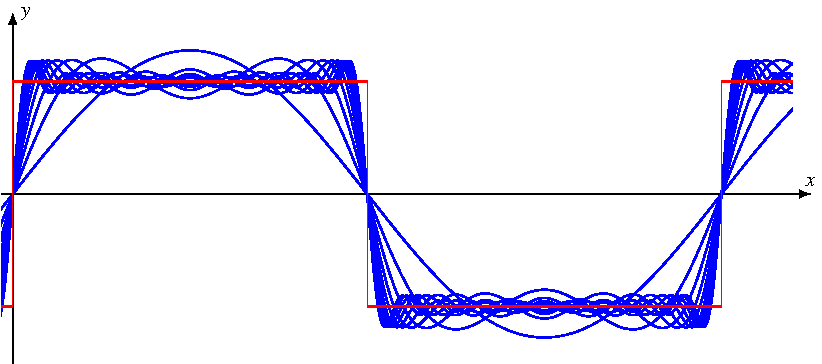
\includegraphics{chapters/010-skalarprodukt/images/fourierrechteck.pdf}
\caption{Approximation der Rechteckfunktion (rot) durch eine Folge
von Partialsummen der Fourier-Reihe.
\label{buch:skalarprodukt:fig:fourierrechteck}}
\end{figure}%
Die Supremum-Norm auf dem Raum der stetigen Funktionen hat den
Begriff der gleichmässig konvergenten Funktionenfolgen ergeben.
Cauchy-Folgen von stetigen Funktionen in der Supremum-Norm konvergieren
wieder gegen eine stetige Funktione.
Ist eine Funktion nicht stetig, lässt Sie sich im Sinne der Supremum-Norm
nicht durch stetige Funktionen approximieren.
Andererseits hat Fourier gezeigt, wie man technische wichtige Funktionen
wie die Rechteckfunktion durch trigonometrische Polynome
\begin{equation}
f_n(x)
=
\frac{4}{\pi} \sum_{k=0}^n \frac{\sin kx}{k}
=
\frac{4}{\pi} \biggl(
\sin x
+
\frac{\sin 3x}{3}
+
\frac{\sin 5x}{5}
+
\frac{\sin 7x}{7}
+
\ldots
\biggr)
\label{buch:skalarprodukt:eqn:rechteckreihe}
\end{equation}
approximieren kann.
Diese sind alle stetig und kommen der Rechteckfunktion in jedem Punkt,
in dem die Funktion stetig ist, beliebig nahe.
An den Stellen $x = n\pi$ hat die Grenzfunktion eine Sprungstelle,
die approximierenden Funktionen haben dort immer Abstand $1$
(siehe Abbildung~\ref{buch:skalarprodukt:fig:fourierrechteck}).
Die Folge ist also keine Cauchy-Folge und sie konvergiert nicht im
Sinne der Supremum-Norm.
Für solche Anwendungen muss eine besser geeignete Norm gefunden werden,
in der die Folge konvergiert.

%
% Skalarprodukt von Funktion
%
\subsubsection{Die $L^1$-Norm einer Funktion}
Die Supremum-Norm sieht nur den grössten Wert, die Konvergenz der Folge
\eqref{buch:skalarprodukt:eqn:rechteckreihe} ist aber nicht gleichmässig,
die maximale Abweichung ist immer $1$.
Gesucht ist eine Norm, die für die Folge
\eqref{buch:skalarprodukt:eqn:rechteckreihe} 
nur im Mittel eine Abweichung feststellt.
Für die Berechnung des Mittelwerts kann das Integral verwendet werden:

\begin{definition}
\label{buch:skalaprodukt:definition:l1norm}
Für eine stetige Funktion $X\to\mathbb{R}$, für die $x\mapsto |f(x)|$
integrierbar ist, heisst
\begin{equation}
\|f\|_1 = \int_X |f(x)|\,dx
\label{buch:skalarprodukt:eqn:l1norm}
\end{equation}
die {\em $L^1$-Norm} der Funktion $f$.
\end{definition}

Die $L^1$-Norm ist tatsächlich eine Norm, wir verifizieren die
definierenden Eigenschaften einer Norm.
\begin{enumerate}
\item
Definit: Sei $f$ eine stetige Funktion mit $\|f\|_1=0$
Wäre $f\ne 0$, dann gäbe es einen Punkt $x_0\in X$ mit $f(x_0) \ne 0$.
Da $f$ stetig ist, ist $f|(x)| > \frac12|f(x_0)|$ für $x$ in einer
$\delta$-Umgebung von $x_0$.
Dann folgt für die $L^1$-Norm
\begin{align*}
\|f\|_1
=
\int_X |f(x)|\,dx
\ge
\frac12 |f(x_0)| \cdot \delta 
> 0.
\end{align*}
Dies widerspricht der Annahme, dass $\|f\|_1=0$ ist, also muss $f=0$ sein.
\item
Homogeneität folgt durch direkte Rechnung
\[
\|\lambda f\|_1
=
\int_X |\lambda f(x)|\,dx
=
|\lambda|
\int_X |f(x)|\,dx
=
|\lambda| \cdot \|f\|.
\]
\item
Die Dreiecksungleichung folgt aus
\[
\|f+g\|_1
=
\int_X |f(x) + g(x)|\,dx
\le
\int_X |f(x)| + |g(x)|\,dx
=
\int_X |f(x)| + \int_X |g(x)|\,dx
=
\|f\|_1 + \|g\|_1.
\]
\end{enumerate}

Die $L^1$-Norm ist etwas ``schwächer'' als die Supremum-Norm im
folgenden Sinne.
Eine in der Supremum-Norm konvergente Funktionenfolge auf einem
kompakten Definitionsbereich $X$ ist auch in der $L^1$-Norm konvergent.
Zur Unterscheidung der verschiedenen Normen werden wir in Zukunft die
Supremum-Norm manchmal auch als $\|f\|_{\infty} = \|f\|$ schreiben.

\begin{satz}
Ist $X$ eine kompakte Teilmenge von $\mathbb{R}$ und $f_n$ eine
in der Supremum-Norm konvergente Folge stetiger Funktionen $f_n$,
dann ist $f_n$ auch in der $L^1$-Norm konvergent.
\end{satz}

\begin{proof}
Konvergenz in der Supremum-Norm bedeutet, dass für jedes $\varepsilon>0$
ein $N>0$ existiert derart, dass $|f_n(x)-f(x)|<\varepsilon$ für alle
$x\in X$ und alle $n>N$.
Für die $L^1$-Norm gilt dann
\begin{align*}
\|f_n-f\|_1
&=
\int_X |f_n(x) - f(x)|\,dx
\le
\int_X \varepsilon \,dx
=
\varepsilon \int_X \,dx
=
\varepsilon \operatorname{vol}(X).
\end{align*}
Da für einen kompakten Definitionsbereich $\operatorname{vol}(X)<\infty$
gilt, bedeutet dies, dass die $\|f_n-f\|_1\to 0$, dass also $f_n$ in
der $L^1$-Norm konvergiert.
\end{proof}

\begin{beispiel}
Die Folge $f_n(x)$ von \eqref{buch:skalarprodukt:fig:fourierrechteck}
konvergiert tatsächlich in der $L^1$-Norm auf dem Intervall $[0,2\pi]$.
Zwar ist $f_n$ nicht gleichmässig konvergent, aber fast.
Man kann zeigen, dass für jedes $\delta>0$, die Funktionen
$f_n(x)$ in Punkten $x$, die weiter als $\delta$ von den
Punkten $k\pi$ mit $k\in\mathbb{Z}$, gleichmässig konvergieren.
Innerhalb einer $\delta$-Umgebung der Vielfachen von $\pi$ ist die
$f_n(x)-f(x)$ beschränkt.
Die genaue Schranke ist nicht wichtig, wir nennen sie $M$ und bekommen
\[
|f_n(x)-f(x)|
\le M
\quad\forall x\in X.
\]
Ausserhalb einer kleinen Umgebung konvergiert die Folge gleichmässig,
zu jedem $\varepsilon>0$ gibt es also ein $N>0$ derart, dass
\[
|f_n(x)-f(x)|<\varepsilon
\]
für $x$ weiter als $\delta$ von $k\pi$ entfernt.
Für die $L^1$-Norm folgt dann
\begin{align*}
\|f_n-f\|_1
&=
\int_0^{2\pi} |f_n(x)-f(x)|\,dx
\\
&=
\int_0^\delta |f_n(x)-f(x)|\,dx
+
\int_\delta^{\pi-\delta} |f_n(x)-f(x)|\,dx
+
\int_{\pi-\delta}^{\pi+\delta} |f_n(x)-f(x)|\,dx
\\
&\qquad
+
\int_{\pi+\delta}^{2\pi-\delta} |f_n(x)-f(x)|\,dx
+
\int_{2\pi-\delta}^{2\pi} |f_n(x)-f(x)|\,dx
\\
&\le
\delta M
+
\varepsilon (\pi -2\delta)
+
2\delta M
+
\varepsilon (\pi -2\delta)
+
\delta M
\le
4\delta M + 2\pi\varepsilon
\end{align*}
für $n>N$.
Dadurch, dass man $\delta$ und $\varepsilon$ klein macht, kann man
also immer ein $N$ finden, so dass $\|f_n-f\|_1$ beliebig klein wird
für $n>N$.
Damit ist gezeigt, dass die Folge $f_n$ in der $L^1$-Norm konvergiert.
\end{beispiel}

Das Beispiel zeigt, dass die $L^1$-Norm eine schwäre Form der Konvergenz
ist, die eine erweiterte Klasse von Funktionen durch stetige Funktionen
zu approximieren erlaubt.

%
% Das $L^2$-Skalarprodukt
%
\subsubsection{Das $L^2$-Skalarprodukt}
Die $L^1$-Norm ist weniger strikt als die Supremum-Norm, aber sie ist
immer noch recht weit von der Intuition entfernt, die wir von der
Entfernungsmessung in der Geometrie haben, die von einem Skalarprodukt
herrühren.
Das Beispiel~\ref{buch:skalarprodukt:cauchyschwarz:beispiel:skalarprodukt}
weist den Weg, mit dem wir eine Norm für stetige Funktionen gewinnen
können, die von einem Skalarprodukt herkommt.

\begin{definition}
\label{buch:skalarprodukt:funktionraeume:definition:skalarprodukt}
Das {\em Skalarprodukt} stetiger Funktionen auf $X\subset \mathbb{R}$
ist definiert durch
\begin{equation}
\langle f,g\rangle
=
\int_X f(x)g(x)\,dx.
\label{buch:skalarprodukt:funktionraeume:eqn:skalarprodukt}
\end{equation}
\end{definition}

Es genügt nachzurechnen, dass $\langle f,g\rangle$ die Eigenschaften
eines Skalarproduktes hat, dann folgt die Dreiecksungleichung automatisch.
Zunächst ist klar,
dass~\eqref{buch:skalarprodukt:funktionraeume:eqn:skalarprodukt}
bilinear ist:
\begin{align*}
\langle \lambda f_1+\mu f_2,g\rangle
=
\int_X (\lambda f_1(x) + \mu f_2(x)) g(x)\,dx
&=
\lambda\int_Xf_1(x)g(x)\,dx + \mu\int_X f_2(x)g(x)\,dx
\\
&=
\lambda\langle f_1,g\rangle + \mu\langle f_2,g\rangle
\\
\langle f,\lambda g_1+\mu g_2\rangle
=
\int_X f(x)(\lambda g_1(x)+\mu g_2(x))\,dx
&=
\lambda\int_X f(x)g_1(x)\,dx + \mu\int_X f(x)g_2(x)\,dx
\\
&=
\lambda\langle f,g_1\rangle + \mu\langle f,g_2\rangle.
\end{align*}
Die Bilinearform ist aber auch positiv definit: Für eine stetige
Funktion $f(x)$ gilt
\[
\langle f,f\rangle
=
\int_X f(x)^2\,dx \ge 0.
\]
Da auch $f(x)^2$ eine stetige Funktion ist,
verschwindet das Integral genau dann, wenn $f(x)=0\;\forall x\in X$ ist.

Die zum Skalarprodukt gehörige Norm 
\[
\|f\|_2
=
\int_X |f(x)|^2\,dx
\]
heisst auch die {\em $L^2$-Norm}.

%
% Nicht kompakte Definitionsbereiche
%
\subsubsection{Nicht kompakter Definitionsbereich}
Für stetige Funktionen auf einem kompakten Definitionsbereich scheinen
die drei Normen $\|\;\cdot\;\|_\infty$, $\|\;\cdot\;\|_1$ und
$\|\;\cdot\;\|_2$ zu den gleichen Konvergenzbegriffen zu führen.
In diesem Abschnitt soll gezeigt werden, dass dies für nicht kompakte
Definitionsbereiche nicht mehr gilt.
Nicht einmal die Menge der Funktionen, die eine endliche Norm haben,
ist gleich.

\begin{beispiel}
Auf dem Definitionsbereich $X=(0,1]$ hat die Funktion
$f(x)=\log x$ endliche $L^1$-Norm aber unendliche Supremum-Norm.

\medskip
\noindent
Wegen $\lim_{x\to 0+}\log x = -\infty$ folgt $\|\log\|=\infty$.
Für die $L^1$-Norm folgt mit der Substitution $y=\log x$ und
$dy = dx/x$ oder $dx = e^y\,dy$
\begin{align*}
\|\log\|_1
&=
\int_0^1|\log x|\,dx
=
-\int_0^1\log x\,dx
=
-\int_{-\infty}^0 e^y\,dy
=
-\biggl[ e^y \biggr]_0^{-\infty}
=
1.
\end{align*}
Insbesondere ist die $L^1$-Norm beschränkt.
\end{beispiel}

\begin{beispiel}
Auf dem Definitionsbereich $X=[1,\infty)$ hat die Funktion
$f(x)=1/x$ endliche $L^2$-Norm aber unendlich $L^1$-Norm.

\medskip
\noindent
Die Integrale für die Normen ergeben:
\begin{align*}
\|f\|_1
&=
\int_1^\infty \frac{1}{x}\,dx
&
\|f\|_2^2
&=
\int_1^\infty \frac{1}{x^2}\,dx
\\
&=\biggl[\log x\biggr]_1^\infty
&
&=\biggl[-\frac{2}{x}\biggr]_1^\infty
\\
&=\infty
&
&=2.
\end{align*}
Insbesondere ist die $L^1$-Norm unbeschränkt, die $L^2$-Norm dagegen
beschränkt.
\end{beispiel}

\begin{satz}
Eine stetige Funktion auf einem beschränkten Definitionsbereich $X$
mit endlicher $L^2$-Norm hat auch endliche $L^1$-Norm.
\end{satz}

\begin{proof}[Beweis]
Aus der Cauchy-Schwarz-Ungleichung folgt
\begin{align*}
\int_X |f(x)|\,dx
&=
\langle |f|, 1\rangle
\le
\|f\|_2\cdot \|1\|_2.
\end{align*}
Nach Voraussetzung an die Funktion $f$ ist der erste Faktor beschränkt,
der zweite Faktor ist $\operatorname{vol}(X)$ und nach Voraussetzung
auch beschränkt.
\end{proof}

Die Beispiele zeigen, dass die Existenz der Normen selbst für stetige
Funktionen für nicht kompakten Definitionsbereich nicht garantiert ist.
Die Erweiterung auf nicht stetige Funktionen kann muss daher beschränkt
werden auf eine Klasse von Funktionen, für die die entsprechende Norm
existiert.
Das kann bedeuten, dass nicht alle stetigen Funktionen in Betracht 
kommen und dass neue Funktionen, die nicht stetig sind, als
Grenzwerte auftreten können.

%
% Grenzen des Riemann-Integrals
%
\subsection{Grenzen des Riemann-Integrals}
In den vorangegangenen Rechnungen sind wir immer vom Riemann-Integral
ausgegangen, welches man im Analysisunterricht als erstes kennenlernt.
Man zeigt dort, dass es für stetige Funktionen existiert und für
gleichmässig konvergente Folgen von Funktionen der Grenzwert des
Integrals mit dem Integral des Grenzwertes übereinstimmt:
\[
\int_X \lim_{n\to\infty} f_n(x)\,dx
=
\lim_{n\to\infty}
\int_X f_n(x)\,dx
\]
Der vorangegangene Abschnitt hat gezeigt, dass wir die Klasse der
Funktionen ausdehnen müssen auf Funktionen, die nicht stetig sind,
für die aber immer noch die $L^1$- oder die $L^2$-Norm existiert.
Hier zeigen sich die Schwächen des Riemann-Integrals.
In diesem Abschnitt soll an Beispielen gezeigt werden, was schief
gehen kann, und wie das Problem gelöst werden kann.

%
% Abzählbar viele Stetigkeitsstellen
%
\subsubsection{Abzählbar viele Unstetigkeitsstellen}
Wir konstruieren eine Funktionenfolge von Riemann-integrierbaren 
Funktionen, die alle das Integral $0$ haben, deren Grenzfunktion
aber nicht mehr Riemann-integrierbar ist.

Die rationalen Zahlen im Intervall $[0,1]$ sind abzählbar, d.~h.~es
gibt eine Folge $n\mapsto q_n\in[0,1]\cap\mathbb{Q}$, in der jede
rationale Zahl im Intervall vorkommt.
Aus der Folge $q_n$ konstruieren wir jetzt die Folge von Funktionen
\[
f_n(x)
=
\begin{cases} 
1&\qquad\text{$x$ ist einer der Werte $q_1,q_2,\ldots,q_n$}\\
0&\qquad\text{sonst}.
\end{cases}
\]
Die Funktion $f_n(x)$ ist also an genau $n$ Stellen von $0$ erschieden
und hat dort den Wert $1$.
Das Riemann-Integral ``sieht'' endlich viele Sprungstellen nicht,
die Funktionen $f_n$ sind also alle Riemann-integrierbar und haben
das Integral
\[
\int_0^1 f_n(x)\,dx=0.
\]
Insbesondere ist auch
\[
\lim_{n\to\infty}\int_0^1 f_n(x)\,dx = 0.
\]
Andererseits ist die Grenzfunktion
\begin{equation}
f(x)
=
\begin{cases}
1&\qquad\text{$x\in[0,1]\cap\mathbb{Q}$ ist rational}\\
0&\qquad\text{sonst, $x$ ist irrational.}
\end{cases}
\label{buch:skalarprodukt:funktionenraeume:eqn:ratfunk}
\end{equation}
Das Riemann-Integral der Funktion $f(x)$ existiert nicht.
Dazu müsste man ja für eine Unterteilung $0=x_0<x_1<\dots x_n=1$
die Riemann-Summen
\[
\overline{I}
=
\sum_{k=0}^{n-1}
(x_{k+1}-x_k) \sup_{x_k\le \xi \le x_{k+1}} f(\xi)
\qquad\text{und}\qquad
\underline{I}
=
\sum_{k=0}^{n-1}
(x_{k+1}-x_k) \inf_{x_k\le \xi \le x_{k+1}} f(\xi)
\]
berechnen, und sie müssten bei Verfeinerung der Unterteilung
gegeneinander konvergieren.
Aufgrund der Konstruktion der Funktion $f(x)$ ist aber
\[
\sup_{x_k\le \xi \le x_{k+1}} f(\xi) = 1
\qquad\text{und}\qquad
\inf_{x_k\le \xi \le x_{k+1}} f(\xi) = 0,
\]
sodass
$\overline{I}=1$ und $\underline{I}=0$ ist, ganz unabhängig von
der Unterteilung.

Der Riemannsche Integralbegriff muss also für die Zwecke der Approxmation
mit der $L^1$ oder $L^2$-Norm erweitert werden, so dass er sinnvoll mit
abzählbar vielen Unstetigkeitsstellen umgehenn kann.
Insbesondere sollte er als Integral der Funktion $f(x)$ 
von \eqref{buch:skalarprodukt:funktionenraeume:eqn:ratfunk}
den Wert $0$ liefern.

%
% Masse
%
\subsubsection{Masstheorie}
Gesucht wird also ein Integral, das für eine grössere Klasse von
Funktionen definiert ist und welches sich bezüglich Grenzwerten
besser verhält als das Riemann-Integral.
Das Integral ist nur dann nützlich, wenn es für viele Funktionen
die gleichen Werte ergibt.

Die einfachsten Funktionen, die wir integrieren wollen, sind die
{\em Indikatorfunktionen}, Funktionen, die durch eine Teilmenge
\index{Indikatorfunktion}
$A\subset X$ definiert sind durch
\[
1_A(x)
=
\begin{cases}
1&\qquad\text{für $x\in A$}\\
0&\qquad\text{sonst}.
\end{cases}
\]
Für ein Intervall der Länge $\lambda(A)$ ist
\[
\int_X 1_A(x)\,dx = \lambda(A).
\]
Für Mengen, die sich aus vielen Intervallen zusammensetzen, erwarten wir
die Summenformel
\[
A=\bigcup_{k=1}^\infty A_k,
\quad
A_k\cap A_j = \emptyset\;\forall k\ne j
\qquad\Rightarrow\qquad
\lambda(A) = \sum_{k=1}^\infty \lambda(A_k).
\]
Ausserdem sollte für eine Teilmenge $A\subset B$ der Inhalt der
Differenz $\lambda(A\setminus B)=\lambda(A)-\lambda(B)$ sein.

So entsteht eine Klasse von Mengen, denen sinnvoll ein Inhalt 
zugeordnet werden kann.
Solche Mengen heissen {\em messbar}.
Dazu gehören alle Intervalle, aber auch alle Differenzen und
abzählbaren Vereinigungen von Intervallen und messbaren Mengen
sind wieder messbar.
Die Klasse der messbaren Mengen ist also sehr gross.
Es braucht natürlich noch einiges an Arbeit, um zu zeigen, dass
eine widerspruchsfreie Definition der Funktion $\lambda(A)$
tatsächlich möglich ist, die jeder messbaren Menge einen
Inhalt zuordnet.
Eine solche Funktion heisst ein {\em Mass}, das aus der Intervalllänge
konstruierte Mass heisst auch das Lebesgue-Mass nach Henri Léon Lebesgue..
\index{Lebesgue-Mass}%
\index{Mass}%

Von besonderem Interesse sind Mengen, deren Inhalt $0$ ist.

\begin{definition}
\label{buch:skalarprodukt:funktionenraeume:definition:nullmenge}
Eine Nullmenge bezüglich des Masses $\lambda$ ist eine messbare
Menge $A$ mit Mass $\lambda(A)=0$.
\index{Nullmenge}
\end{definition}

Der Riemannsche Integralbegriff lässt bei der Bestimmung des Masses
nur endlich viele Intervalle zu. 
Die Menge $Q$ der rationalen Zahlen im Intervall $[0,1]$ ist abzählbar
unendlich.
In jeder beliebigen Umgebung einer reellen Zahl in $[0,1]$ findet man
rationale Zahlen in $Q$, eine Überdeckung der Menge der rationalen
Zahlen mit endlich vielen Intervallen enthält daher immer auch alle
reellen Zahlen, mit der möglichen Ausnahme von endlich vielen Zahlen.
Der Inhalt, den der Riemannsche Integralbegriff der Menge $Q$ zuordnen
muss, ist daher $1$.

Der neue Massbegriff erlaubt, die Menge mit abzählbar vielen messbaren
Mengen zu überdecken.
Sei $q_k$ eine Folge, die alle rationalen Zahlen in $Q$ durchläuft.
Zu jedem $k$ konstruieren wir das Intervall
\[
A_k = (q_k-\varepsilon2^{-k},q_k+\varepsilon2^{-k})
\]
mit Inhalt $\lambda(A_k) = 2\varepsilon2^{-k}$.
Es ist klar, dass die Intervalle $A_k$ die ganze Menge $Q$ überdecken,
also
\[
Q\subset \bigcup_{k=1}^\infty A_k.
\]
Der Inhalt der Menge $Q$ ist daher
\[
\lambda(Q)
\le
\sum_{k=1}^\infty \lambda(A_k)
=
\sum_{k=1}^\infty 2\varepsilon 2^{-k}
=
2\varepsilon
\sum_{k=1}^\infty 2^{-k}
=
2\varepsilon.
\]
Da $\varepsilon$ beliebig klein gewählt werden kann, folgt, dass
$\lambda(Q)=0$ sein muss.
Aus diesem Beispiel lässt sich erahnen, dass der Lebesguesche Massbegriff
mit Grenzwerten besser umgehen kann als der aus dem Riemannschen Integral
abgeleitete.

%
% Lebesgue-Integral
%
\subsubsection{Lebesgue-Integral}
Aus der Konstruktion eines Masses $\lambda$ kann jetzt die Konstruktion
eines Integrals an die Hand genommen werden.
Dazu werden Funktionen durch Stufenfunktionen approximiert, die
von der Form
\[
f(x) = \sum_{k=1}^\infty a_k 1_{A_k}(x)
\]
sind, wobei $A_k$ messbare Mengen sind.
Für solche Funktionen ist die naheliegende Definition des Integrals
\[
\int_X f(x)\,d\lambda(x)
=
\sum_{k=1}^\infty a_k \lambda(A_k).
\]
Der wesentliche Unterschied zur Riemannsschen Konstruktion ist,
dass nicht nur Intervalle zulässig sind sondern beliebige messbare Mengen.
Die Berechnung des Inhalts einer messbaren Mengen beinhaltet bereits
die Möglichkeit, Grenzwerte zu bilden.
Auch hier ist viel Arbeit notwendig um nachzuweisen, dass sich aus diesem
Ansatz ein widerspruchsfreier neuer Integralbegriff ergibt.
Das so konstruierte Integral heisst das {\em Lebesgue-Integral} und
\index{Lebesgue-Integral}%
wird zur Unterscheidung vom gewöhnlichen Riemannschen Integral und
wegen der Bedeutung des Masses $\lambda$, welches eine grosse Rolle
bei seiner Konstruktion spielt mit
\[
\int_X f(x) \,d\lambda(x)
\]
bezeichnet.

Beim Riemannschen Integral haben endliche Mengen und Mengen mit endlich
vielen Häufungspunkten Inhalt $0$.
Viele abzählbare Mengen haben dagegen positiven Inhalt.
Das Lebesguesche Mass gibt allen abzählbaren Mengen den Inhalt 0.

Unterscheiden sich zwei Funktionen $f$ und $g$ nur auf einer Nullmenge,
sagt man, sie seien {\em fast überall} gleich, geschrieben
\[
f(x) = g(x) \qquad \text{fast überall}.
\]
Zwei fast überall gleiche Funktionen haben das gleiche Integral, denn
\[
\int_X f(x)\,dx - \int_X g(x)\,dx
=
\int_X f(x)-g(x)\,dx
=
\int_X 0\,dx=0
\]
weil das Integral einer fast überall verschwindenden Funktion $0$ ist.

%
% Funktionsklassen
%
\subsubsection{Klassen von fast überall gleichen Funktionen}
Verwendet man die mit dem Lebesgque-Integral berechnete $L^1$- oder
$L^2$-Norm, dann können Funktionen nicht voneinander unterschieden werden,
die fast überall gleich sind.
Grenzwerte von Funktionenfolgen in der $L^1$- oder $L^2$-Norm sind
daher nur bis auf eine Nullmenge bestimmt.

\begin{definition}
Die Menge der Lebesgue-integrierbaren Funktionen auf dem Definitionsbereich
$X\subset\mathbb{R}$ wird mit
\[
\mathscr{L}^1(X)
=
\mathscr{L}^1_{\mathbb{R}}(X)
=
\left\{ f\colon X\to \mathbb{R}
\;\left|\;
\text{$f$ ist $\lambda$-integrierbar und $\int_X|f(x)|\,dx< \infty$}
\right.\right\}
\]
bezeichnet.
Entsprechend besteht $\mathscr{L}^2(X)$ aus den Funktionen $X\to \mathbb{R}$,
für die $|f(x)|^2$ integrierbar ist.
Sie heissen auch die {\em quadratintegrierbaren} Funktionen.
\end{definition}

Das Lebesgue-Integral kann Funktionen, die sich nur auf einer Nullmenge
verschieden sind, nicht unterscheiden. 
Daher ist es notwenig, solche Funktionen in Klassen zusammenzufassen:

\begin{definition}
Die Relation
\[
f\sim g
\qquad:\Leftrightarrow \qquad f(x) = g(x)\quad\text{fast überall}
\]
ist eine Äquivalenzrelation.
Die Menge der Äquivalenzklassen von Funktionen in $\mathscr{L}^1(X)$
bezüglich dieser Relation werden mit $L^1(X)$ bezeichnet, ebenso werden
die Äquivalenzklassen von $\mathscr{L}^2(X)$ bezüglich der Relation $\sim$
mit $L^2(X)$ bezeichnet.
\end{definition}

Mit den Funktionsklassen in $L^1(X)$ und $L^2(X)$ lässt sich genau
so rechnen, wie man es sicht gewohnt ist.
Für die Summe von Funktionen $f_1\sim f_2$ und $g_1\sim g_2$ gilt
\[
\left.
\begin{aligned}
f_1(x)&=f_2(x)&&\text{fast überall}\\
g_1(x)&=g_2(x)&&\text{fast überall}\\
\end{aligned}
\quad
\right\}
\qquad
\Rightarrow
\qquad
f_1(x)+g_1(x) = f_2(x)+g_2(x)\quad\text{fast überall},
\]
denn die Menge, auf der sich $f_1+f_2$ und $g_1+g_2$ unterscheiden
ist höchstens die Vereinigung der Mengen, auf denen sich $f_1$ und 
$f_2$ bzw.~$g_1$ und $g_2$ unterscheiden.
Die Vereinigung von Nullmengen ist aber wieder eine Nullmenge.

%
% Lebesgue-Integral
%
\subsubsection{Dominierte Konvergenz}
Die Entwicklung des Lebesgueschen Integrallbegriffs war motiviert
vom Wunsch, ein Integral zu erhalten, welches sich bezüglich
Konvergenz von Funktionenfolgen besser verhält.
Tatsächlich liefert die Theorie den folgenden zentralen Satz.

\begin{satz}[Dominierte Konvergenz]
\label{buch:skalarprodukt:satz:dominierte-konvergenz}
Sei $f_n$ eine auf dem Definitionsbereich $X$ punktweise konvergente
Folge Lebesgue-integrierbarer Funktionen mit Grenzfunktion 
\[
f(x) = \lim_{n\to \infty} f_n(x).
\]
Sei ausserdem $g$ eine Lebesgue-integrierbare Funktion mit
$|f_n(x)|<g(x)$ für alle $x\in X$.
Dann ist $f$ Lebesgue-integrierbar und es gilt
\[
\lim_{n\to\infty} \int_X f(x)\,d\lambda(x)
=
\int_X f(x)\,d\lambda(x)
\]
\end{satz}

Der Satz der dominierten Konvergenz von Lebesgue ersetzt also die
Bedingung der gleichmässigen Konvergenz, die beim Riemann-Integral
erfolgreich war, durch die viel schächere Bedingung, dass alle
Funktionen unterhalb einer gemeinsamen integrierbaren Funktion bleiben.
Dadurch wird verhindert, dass die Funktionen $f_n$ nach $\infty$
``ausbrechen'' kann und gegen eine Funktion konvergieren, die nicht
mehr integrierbar ist.


%
% Berechnung von Lebesgue-Integralen
%
\subsubsection{Berechnung von Lebesgue-Integralen}
Das Lebesque-Integral löst also die technischen Probleme, die das
Riemann-Integral manchmal bei Funktionenfolgen hat, die gegen ein
Grenzfunktion konvergieren, der man ein sinnvolles Integral im
Lebesgueschen Sinnen zuordnen kann.
Doch wie berechnet man ein Lebesgue-Integral?

Stetige Funktionen lassen sich beliebig genau durch Treppenfunktionen
approximieren.
Die Konvergenz des Lebesgue-Integrals für solche Funktionenfolgen
garantiert daher, dass das Lebesgue-Integral für stetige
Funktionen mit dem Riemann-Integral übereinstimmt.
Insbesondere braucht es keinen neuen Formalismus für die 
Berechnung von Integralen.
Auch für Funktionen, die an höchstens endlich vielen Stellen unstetig
sind, stimmt das Riemann-Integral mit dem Lebesgue-Integral überein.

Man soll sich daher das Lebesgue-Integral vor allem als eine 
Erweiterung des Integrals auf Funktionen vorstellen, die als Grenzwerte
von Folgen stetiger Funktionen im Sinne der $L^1$- oder der $L^2$-Norm
auftreten können.
Stetigkeit kann dabei verloren gehen, aber Konvergenzeigenschaften
wie die dominierte Konvergenz von
Satz~\ref{buch:skalarprodukt:satz:dominierte-konvergenz}
bleiben erhalten.




%
% 4-hilbertraum.tex
%
% (c) 2022 Prof Dr Andreas Müller, OST Ostschweizer Fachhochschule
%
\section{Hilbert-Raum
\label{buch:skalarprodukt:section:hilbertraum}}
\kopfrechts{Hilbert-Raum}
Ein Skalarprodukt stattet einen Vektorraum mit einer Norm aus.
Es ermöglicht auch, orthonormierte Vektoren zu finden.
In endlichdimensionalen Vektorräumen können so besonders nützliche
Basen konstruiert werden.
In den Funktionenräumen von
Abschnitt~\ref{buch:skalarprodukt:section:funktionenraeume},
die unendlichdimensional sind, kann der Orthonormalisierungsprozess
ohne Ende weitergeführt werden.
Im Gegensatz zu einem endlichdimensionalen Vektorraum bilden diese
orthonormierten Vektoren keine Basis, denn nicht jeder Vektor lässt
sich als Linearkombination schreiben.
Dies wird erst mit Hilfe von Reihenentwicklungen möglich, doch dazu
müssen Fragen der Konvergenz solcher Reihen geklärt werden.
Der in diesem Abschnitt eingeführte Begriff des Hilbert-Raumes tut dies.

%
% Prähilbertraum
%
\subsection{Prähilbertraum}
Die Funktionenräume, in denen wir harmonische Analysis betreiben wollen,
zeichnen sich durch das Vorhandensein eines Skalarproduktes aus.
Wir fassen diese Eigenaschaften im Begriff des Prähilbertraumes
zusammen.

\begin{definition}
Ein reeller Prähilbertraum ist ein reller Vektorraum mit einem
(reellen) Skalarprodukt.
\index{Prähilbertraum}%
Eine komplexer Prähilbertraum ist ein komplexer Vektorraum mit einem
sesquilinearen Skalarprodukt.
\end{definition}

\begin{beispiel}
Der endlichdimensionale reelle Vektorraum $\mathbb{R}^n$ ist ein
reller Prähilbertraum mit dem Skalarprodukt
\[
\langle u,v\rangle
=
\sum_{i=1}^n u_iv_i
\]
für Vektoren $u,v\in\mathbb{R}^n$.
\end{beispiel}

\begin{beispiel}
Der endlichedimensionale komplexe Vektorrau $\mathbb{C}$ ist ein
komplexer Prähilbertraum mit dem Skalarprodukt
\[
\langle u,v\rangle
=
\sum_{i=1}^n \overline{u}_iv_i
\]
für Vektoren $u,v\in\mathbb{C}^n$.
\end{beispiel}

Die Skalarprodukte in den Beispielen sind nicht die einzig möglichen
Skalarprodukte.
Alternative Skalarprodukte auf einem reellen Prähilbertraum können 
durch eine beliebige positiv definite Matrix $A$ durch
\[
\langle u,v\rangle_A
=
\sum_{i,j=1}^n u_ia_{ij}v_j
\]
definiert werden.
Wir schreiben die aus $\langle\;,\;\rangle_A$ abgeleitete Norm mit
$\normfunc_A$.
Solange unser primäres Interesse der Approximation von Funktionen gilt,
kommt es vor allem darauf an, dass die Norm, die aus dem Skalarprodukt
abgeleitet wird, zu den gleichen konvergenten Folgen führen.
Die Funktion $u\mapsto \|u\|_A$ ist stetig, sie hat daher auf der
Einheitskugel des Prähilbertraumes ein Maximum und eine Minimum,
welches wir mit $M$ bzw.~$m$ bezeichen.
Dann folgt, dass
\[
m\|u\|\le \|u\|_A\le M\|u\|
\]
für beliebige Vektoren $u\in\mathbb{R}^n$.
Daraus kann man jetzt ableiten, dass die beiden Normen $\normfunc$
und $\normfunc_A$ auf die gleichen Cauchy-Folgen und die gleichen
konvergenten Folgen führen.
Wir zeigen dies für Cauchy-Folgen:
\begin{enumerate}
\item
Sei $u_k$ eine Cauchy-Folge bezüglich der Norm $\normfunc$,
und $\varepsilon>0$.
Wir müssen zeigen, dass $u_k$ auch eine Cauchy-Folge ist bezüglich
der Norm $\normfunc_A$.
Da $u_k$ eine Cauchy-Folge bezüglich der Norm $\normfunc$ ist,
gibt es ein $N>0$ derart, dass
$\|u_k-u_l\|<\varepsilon/M$ für $k,l>N$.
Dann folgt aber
\[
\|u_k-u_l\|_A
\le
M\|u_k-u_l\|
<
M\frac{\varepsilon}{M}
=
\varepsilon
\]
für $k,l>N$.
Somit ist $u_k$ eine Cauchy-Folge bezüglich der Norm $\normfunc_A$.
\item
Ist umgekehrt  $u_k$ eine Cauchy-Folge bezüglich der Norm $\|\,\cdot\,\|_A$,
dann gibt es ein $N>0$ derart, dass $\|u_k-u_l\|_A<m\varepsilon$ ist für
$k,l>N$.
Dann folgt
\[
m\|u_k-u_l\|\le \|u_k-u_l\|_A < m\varepsilon
\qquad\Rightarrow\qquad \|u_k-u_l\|<\varepsilon
\]
für $k,l>N$, also ist $u_k$ auch eine Cauchy-Folge bezüglich der Norm
$\|\,\cdot\,\|$.
\end{enumerate}
In einem endlichdimensionalen Prähilbertraum hat die Wahl des Skalarproduktes
keinen Einfluss darauf, ob eine Folge eine Cauchy-Folge ist oder nicht.
Orthonormierte Vektoren werden natürlich im Allgemeinen nicht mehr
orthonormiert, dies ist jedoch ein Aspekt, dem wir uns erst später
zuwenden werden.

%
% Orthonormierte Vektoren
%
\subsection{Orthonormierte Vektoren in einem Prähilbertraum}
Der Gram-Schmidt-Orthogonalisierungsprozess kann auf eine beliebige
\index{Gram-Schmidt}%
linear unabhängige Menge von Vektoren in einem Prähilbertraum angewendet
werden.
Aus den linear unabhängigen Vektoren $a_1,a_2,\dots$ werden die
orthonormierten Vektoren
\begin{align*}
b_1
&=
\frac{a_1}{\|a_1\|}
\\
b_2
&=
\frac{
a_2 - \langle b_1,a_2\rangle b_1
}{
\|a_2 - \langle b_1,a_2\rangle b_1\|
}
\\
&\phantom{i}\vdots
\\
b_n
&=
\frac{\displaystyle
a_n - \sum_{k=1}^{n-1} \langle b_k,a_n\rangle b_k
}{\displaystyle
\biggl\|a_n - \sum_{k=1}^{n-1} \langle b_k,a_n\rangle b_k\biggr\|
}.
\end{align*}

In einem endlichdimensionalen Vektorraum der Dimension $n$ bricht
der Prozess ab, sobald eine orthonormierte Basis $b_1,\dots,b_n$
aus $n$ Vektoren gefunden wurde.
Jeder andere Vektor $v$ lässt sich dann als Linearkombination
\begin{equation}
v
=
\langle b_1,v\rangle b_1 + \langle b_2,v\rangle b_2 + \dots
=
\sum_{k=1}^n \langle b_1,v\rangle b_1
\label{buch:skalarprodukt:hilbertraum:synthese}
\end{equation}
schreiben.
Da die Summe auf der rechten Seite endlich ist, entstehen keine
Bedenken bezüglich Konvergenz, wie das bei einer unendlichen
Reihe der Fall wäre.

%
% Vollständigkeit
%
\subsection{Vollständigkeit}
In einem unendlichdimensionalen Prähilbertraum bricht der
Orthogonalisierungsprozess nicht ab, es gibt immer noch einen
linear unabhängigen Vektor, der nicht in dem von den bereits
gefundenen Vektoren aufgespannten Raum liegt.
Die Summe~\ref{buch:skalarprodukt:hilbertraum:synthese} wird dann
eine unendliche Summe, die nur im Sinne eines Grenzwertes der
Partialsummenfolge
\begin{equation*}
s_n = \sum_{k=1}^n \langle b_k,v\rangle b_k
\end{equation*}
ausgewertet werden kann.
Man darf zwar aufgrund der Konstruktion aus $v$ davon ausgehen,
dass $s_n$ gegen $v$ konvergiert,
aber für eine beliebige Folge von Koeffizienten $c_k$ ist nicht
garantiert, dass die Summe
\[
\sum_{k=1}^\infty c_kb_k
=
\lim_{n\to\infty} \sum_{k=1}^n c_kb_k
\]
einen Grenzwert hat.
Ein nützliche Theorie kann nur entstehen, wenn gefordert wird,
dass jede Cauchy-Folge des Prähilbertraums tatschächlich konvergiert.

\begin{definition}
Ein Prähilbertraum heisst {\em Hilbert-Raum}, wenn er vollständig ist.
\end{definition}

Endlichdimensionale Vektorräume über sind automatisch vollständig,
da gibt es also gar keinen Unterschied zwischen Prähilbertraum und
Hilbert-Raum.
Das folgende Beispiel zeigt, dass dies für unendlichdimensionale
Hilbert-Räume nicht mehr zutrifft.

\begin{beispiel}
\label{buch:skalarprodukt:hilbertraum:bsp:sinreihe}
Der Funktionenraum
\(
C_{\mathbb{R}}([-\pi,\pi])
\)
der stetigen Funktionen auf dem Intervall $[-\pi,\pi]$ wird mit
dem Skalarprodukt
\[
\langle f,g\rangle
=
\int_{-\pi}^\pi f(x)g(x)\,dx
\]
zu einem Prähilbert-Raum.
Die Summanden der Reihe~\eqref{buch:skalarprodukt:eqn:rechteckreihe} 
sind Sinus-Funktionen, von denen wir später zeigen werden, dass sie
orthogonal sind.
Seien $s_n(x)$ die Partialsummen der Reihe, also
\begin{equation}
s_n(x) = \frac{4}{\pi}\sum_{k=0}^n \frac{\sin (2k+1)x}{2k+1},
\label{buch:skalarprodukt:hilbertraum:eqn:sn}
\end{equation}
dann kann man auch die Norm $\|s_n-s_m\|$, es gilt nämlich
\begin{equation}
\|s_n-s_m\|
=
\biggl\|
\frac{4}{\pi}
\sum_{k=m}^n \frac{\sin (2k+1)x}{2k+1}
\biggr\|,
\label{buch:skalarprodukt:hilbertraum:eqn:snsm}
\end{equation}
wobei wir $n>m$ angenommen haben, was wir ohne Beschränkung der 
Allgemeinheit tun dürfen.
Die Norm eines einzeln Terms ist
\begin{align}
\|\sin rx\|^2
&=
\int_{-\pi}^\pi \sin^2 rx\,dx
=
\int_{-\pi}^\pi \frac12 - \frac{\cos rx}{2}\,dx
=
\int_{-\pi}^\pi \frac12\,dx - \int_{-\pi}^\pi \frac{\cos rx}{2}\,dx.
\notag
\intertext{Der zweite Term ist ein Integral über eine Periode des
Integranden und verschindet daher.
Der erste Term ergibt daher}
\|\sin rx\|^2
&= \pi.
\intertext{Für die Terme der Summe
\eqref{buch:skalarprodukt:hilbertraum:eqn:sn}
folgt daher}
\biggl\|
\frac{\sin{2k+1}x}{2k+1}
\biggr\|^2
&=
\frac{\pi}{(2k+1)^2}.
\notag
\intertext{Für die Differenz
\eqref{buch:skalarprodukt:hilbertraum:eqn:snsm} finden wir daher}
\|s_n-s_m\|^2
\notag
&=
\frac{16}{\pi^2}
\sum_{k=m}^m \frac{\pi}{(2k+1)^2}
=
\frac{16}{\pi}
\sum_{k=m}^m \frac{1}{(2k+1)^2}.
\label{buch:skalarprodukt:hilbertraum:eqn:bsprest}
\end{align}
Da aus dem Analysisunterricht bekannt ist, dass die Reihe $\sum_k\frac1{k^2}$
konvergiert, kann die rechte Seite von 
\eqref{buch:skalarprodukt:hilbertraum:eqn:bsprest}
beliebig klein gemacht werden, die 
Reihe~\eqref{buch:skalarprodukt:eqn:rechteckreihe} 
ist also eine Cauchy-Folge im Prähilbertraum $C_{\mathbb{R}}([-\pi,\pi])$.
Die Grenzfunktion ist die Rechteckfunktion von
Abbildung~\ref{buch:skalarprodukt:fig:fourierrechteck}, sie ist nicht
stetig.
Wir haben also eine Cauchy-Folge im Prähilbertraum 
$C_{\mathbb{R}}([-\pi,\pi])$ gefunden, die darin nicht konvergiert.
\end{beispiel}

%
% Hilbert-Basis
%
\subsection{Hilbert-Basis}
Sei jetzt $H$ ein Hilbert-Raum.
Führt man wieder die Konstruktion einer orthonormierten Basis durch,
entsteht eine Menge $\mathcal{B}=\{b_1,b_2,\dots\}$ orthonormierter
Vektoren.
In einem unendlichdimensionalen Hilbert-Raum ist $\mathcal{B}$ eine
undendliche Menge.
Die Vollständigkeit des Hilbert-Raumes garantiert, dass jede
Cauchy-Folge konvergiert, insbesondere können wir zu jedem beliebigen
Vektor $v$ die Koeffizienten $c_k=\langle b_k,v \rangle$ bestimmen
und versuchen, mit der
Summe~\eqref{buch:skalarprodukt:hilbertraum:synthese}
den Vektor zurückzugewinnen.
Vollständigkeit garantiert zwar die Konvergenz gegen einen Grenzwert
\[
v_0 = \sum_{k=1}^\infty c_k b_k,
\]
aber es gibt keine Garantie, dass $v=v_0$ ist.

\begin{beispiel}
Die Funktionen
\[
b_k(x) = \sin (2k+1)x
\qquad\text{mit}\quad
k\in \mathbb{N}
\]
wurden in Beispiel~\ref{buch:skalarprodukt:hilbertraum:bsp:sinreihe}
die Rechteckfunktion synthetisiert.
Doch reichen diese Funktionen nicht aus, um alle Funktionen auf
dem Intervall $[-\pi,\pi]$ zu synthetisieren.

Für die konstante Funktion $v(x)$ sind die Koeffizienten
\[
\langle v,b_k\rangle
=
\int_{-\pi}^\pi v(x)b_k(x)\,dx
=
\int_{-\pi}^\pi \sin (2k+1)x\,dx
=
0,
\]
die Summe
\[
v_0
=
\sum_{k=0}^\infty
c_k
b_k(x)
=
0
\]
verschwindet also, $v\ne v_0$.
\end{beispiel}

Wir berechnen das Skalarprodukt 
\[
\langle v-v_0,b_k\rangle
=
\langle v,b_k\rangle
-
\biggl\langle \sum_{l=1}^\infty c_lb_l,b_k\biggr\rangle
=
c_k - \sum_{l=1}^\infty c_l\langle b_l,b_k\rangle
=
c_k - \sum_{l=1}^\infty c_l\delta_{lk}
=
c_k-c_k=0.
\]
Der Vektor $v-v_0$ muss also orthogonal sein zu allen Vektoren
$b_k$.
Die Menge der Vektoren $b_k$ kann also vergrössert werden um einen
weiteren Vektor, der zu allen vorhandenen Vektoren orthogonal ist.

\begin{satz}
Eine Menge von orthogonalen Vektoren in einem Prähilbertraum ist linear 
unabhängig.
\end{satz}

\begin{proof}[Beweis]
Angenommen, die orthogonalen Vektoren  $a_1,\dots,a_n$ sind linear
abhängig.
Dann gibt es Zahlen $\lambda_i$, die nicht alle $=0$ sind und derart,
dass
\[
\sum_{k=1}^n \lambda_ka_k
=
\lambda_1 a_1 + \ldots + \lambda_n a_n
=
0.
\]
Das Skalarprodukt mit $a_k$ ergibt
\[
0
=
\langle a_k,\lambda_1a_1 +\ldots + \lambda_na_n\rangle
=
\lambda_1
\langle a_k,a_1\rangle
+
\ldots
+
\lambda_n
\langle a_k,a_n\rangle
=
\lambda_k \|a_k\|^2
\]
für alle $k=1,\dots,n$.
Da die Vektoren $a_k\ne 0$ sind folgt, dass $\lambda_k=0$ sein muss
für alle $k=1,\dots,n$, im Widerspruch zur Voraussetzung, dass die
$\lambda_k$ nicht alle verschwinden.
Der Widerspruch zeigt, dass die Annahme der linearen Abhängigkeit
falsch ist.
\end{proof}

In einem endlichdimensionalen Prähilbertraum findet man immer eine
orthonormierte Basis, aus der sich jeder Vektor linear kombinieren
lässt.
In einem unendlichdimensionalen Raum muss dieser Begriff etwas 
erweitert werden.

\begin{definition}
Eine {\em Hilbert-Basis} des Hilbert-Raumes $H$ ist eine Menge von orthonormalen
\index{Hilbert-Basis}%
Vektoren $b_k\in H$, $k\in \mathbb{N}$ derart, für jeden Vektor $v\in H$
die Reihe 
\[
\sum_{k\in\mathbb{N}} \langle b_k,v\rangle b_k
\]
konvergiert und die Summe $v$ hat.
\end{definition}

Auf eine Hilbert-Basis ist die Inuition anwendbar, die man von 
einer orthonormierten Basis eines endlichdimensionalen Prählibertraumes
hat.

\begin{definition}
\index{separabel}%
Ein Hilbert-Raum, der eine Hilbert-Basis besitzt, heisst {\em separabel}.
\end{definition}

Nicht separable Hilbert-Räume sind deutlich grösser.
In einem nicht separable Hilbert-Raum ist es nicht möglich, alle Vektoren
aus einer Folge von orthonormierten Vektoren linear zu kombinieren.
Dies verträgt sich nicht mit der Intuition, die in endlichdimensionalen
Vektorräumen entstanden ist.
Separabilität ist eine Art ``Endlichkeitseigenschaft''.
Man findet sie zum Beispiel bei den $L^2$-Räumen mit kompaktem
Definitionsgebiet.
Kompaktheit kann als eine topologische
Endlichkeitseigenschaft angesehen werden.
Es lassen sich aber auch nicht separable Hilbert-Räume konstruieren,
zum Beispiel sogenannte fastperiodische Funktionen.
\index{fastperiodische Funktionen}%
Für unsere Anwendungen sind nicht separable Hilbert-Räume jedoch nicht
notwendig und wir können im folgenden annehmen, dass alle Hilbert-Räume
separabel sind und somit eine Hilbert-Basis haben.

%
% Der Hilbert-Raum $l^2$
%
\subsection{Der Hilbert-Raum $l^2$}
Die abstrakte Definition eines separablen Hilbert-Raumes suggeriert,
dass es sehr viele verschiedene Hilbert-Räume geben könnte.
Dem ist aber nicht so, ein Hilbert-Raum ist eine ziemlich starre Struktur.
In diesem Abschnitt konstrieren wir zunächst den besonders übersichtlichen
separablen Hilbert-Raum $l^2$ und zeigen anschliessend, dass sich jeder
separable Hilbert-Raum isometrisch auf $l^2$ abbilden lässt.

\begin{satz}
Der Vektorraum der unendlichen Folgen
\[
l^2_{\mathbb{R}}
=
\biggl\{
(x_0,x_1,\dots)
\in
\mathbb{R}^{\mathbb{N}}
\,\bigg|\,
\sum_{i=0}^\infty x_i^2<\infty\biggr\}
\}
\]
mit dem Skalarprodukt
\[
\langle x,y\rangle_2
=
\sum_{k=0}^\infty x_ky_k
\]
ist ein separabler Hilbert-Raum.
\end{satz}

\begin{proof}[Beweis]
Die Standardbasis des Vektorraums $l^2$ besteht aus den Vektoren $e_i$
mit $i\in\mathbb{N}$ mit 
\begin{align*}
e_0 &= (1,0,0,0,\dots)
\\
e_1 &= (0,1,0,0,\dots)
\\
e_2 &= (0,1,0,0,\dots)
\\  &\;\vdots
\end{align*}
Es ist klar, dass die Vektoren $e_i$ orthonormiert sind.
Wir müssen uns überlegen, dass jede Folge in $l^2$ durch Linearkombinationen
approximiert werden kann.
Wäre das nicht so, dann gäbe es einen von $0$ verschiedenen
Vektor $v=(v_0,v_1,v_2,\dots)\in l^2$, der auf allen Vektoren $e_i$
orthogonal ist.
Dann wäre aber $0=\langle v,e_i\rangle = v_i$, d.~h.~Vektor $v$ ist der
Nullvektor.
Dieser Widerspruch zeigt, dass die Vektoren $e_i$ eine Hilbert-Basis
bilden.
\end{proof}

Der Hilbert-Raum $l^2$ ist die einfachste, direkte Verallgemeinerung der
endlichdimensionalen Hilbert-Raume $\mathbb{R}^n$ mit dem Standardskalarprodukt.
Er ist aber auch der ``einzige'' separable Hilbert-Raum, alle Hilbert-Räume
lassen sich isometrisch auf $l^2$ abbilden.

\begin{satz}
\label{buch:skalarprodukt:hilbertraum:satz:phil2}
Ist $H$ ein separabler Hilbert-Raum, dann gibt es eine isometrische
lineare Abbildung $\varphi\colon H\to l^2$.
\end{satz}

\begin{proof}[Beweis]
Da $H$ separabel ist, gibt es eine Hilbert-Basis $b_0,b_1,b_2,\ldots\in H$
und $v$ ein beliebiger Vektor mit der Darstellung
\[
v = \sum_{k=0}^\infty c_kb_k.
\]
Das Skalarprodukt mit $b_k$ ist
\[
\langle b_i,v\rangle
=
\biggl\langle b_i,\sum_{k=0}^\infty c_kb_k\biggr\rangle
=
\sum_{k=0}^\infty c_k \underbrace{\langle b_i,b_k\rangle}_{\delta_{ik}}
=
c_i.
\]
Die Abbildung
\[
\varphi\colon H \to l^2
:
v \mapsto (\langle b_0,v\rangle,\langle b_1,v\rangle,\langle b_2,v\rangle,\dots)
=
(c_0,c_1,c_2,\dots)=c\in l^2
\]
ist linear und umkehrbar durch die Abbildung
\[
\varphi^{-1} \colon l^2 \to H
:
(c_0,c_1,c_2,\dots) \mapsto \sum_{k=0}^\infty c_k b_k.
\]
Die Norm von $v$ ist
\[
\|v\|^2
=
\biggl\|
\sum_{k=0}^\infty c_k b_k
\biggr\|^2
=
\sum_{k=0}^\infty c_k^2
=
\|c\|_2^2.
\qedhere
\]
\end{proof}

Man verliert also nichts, wenn man statt im Hilbert-Raum $H$ im
Hilbert-Raum $l^2$ rechnet.
Die später zu besprechende Fourier-Transformation ist genau
so eine Abbildung $\varphi$ wie in
Satz~\ref{buch:skalarprodukt:hilbertraum:satz:phil2}, wenn 
trigonometrische Funktionen als Basisfunktionen des Raumes
$L^2([-\pi,\pi])$ verwendet werden.
Die Tatsache, dass die Abbildung eine Isometrie ist, hat einen
speziellen Namen.

\begin{definition}
\label{buch:skalarprodukt:hilbertraum:def:parseval}
Die Identität
\[
\|v\|^2 = \|\varphi(v)\|_2^2
\]
heisst {\em Parseval-Gleichung}.
Aus der Polaridentität folgt dann auch die
{\em Parseval-Plancherel-Formel}
\[
\langle u,v\rangle_H
=
\langle\varphi(u),\varphi(v)\rangle_2
=
\sum_{k=0}^\infty
\langle b_k,u\rangle
\langle b_k,v\rangle.
\]
\end{definition}

Die endlichdimensionalen Hilbert-Räume können auf
natürliche Art in $l^2$ eingebettet werden, indem die Koordinaten
eines $n$-dimensionalen Vektors auf die ersten $n$-Komponenten der
Folge in $l^2$ abgebildet werden.
Aus dieser Idee lässt sich auch ein Prähilbertraum konstruieren,
in dem einfacher gerechnet werden kann.

\begin{definition}
\label{buch:skalarprodukt:hilbertraum:def:l0}
Sei 
\[
l_0
=
\{
x\in \mathbb{R}^{\mathbb{N}}
\mid
\text{$x_k\ne 0$ nur für endlich viele $k$}
\}
\]
der Vektorraum der Folgen, die nur endlich viele nicht verschwindende
Folgenglieder haben.
Die Standardbasisvektoren von $l^2$ sind alle in $l_0$.
\end{definition}

Da die Norm eines Elementes $x\in l_0$ eine endliche Summe ist,
ist $x\in l^2$ und damit $l_0\subset l^2$.
Jeder Vektor $v\in l^2$ kann aber beliebig genau durch einen Vektor
in $l_0$ approximiert werden.
Dazu konstruiert man die Folge
\bgroup
\def\el#1{\phantom{v_0}\llap{#1}}
\begin{align*}
x_0 &= (v_0,\el{0},\el{0},\el{0},\el{0},\dots) \in l_0\\
x_1 &= (v_0,v_1,\el{0},\el{0},\el{0},\dots) \in l_0\\
x_2 &= (v_0,v_1,v_2,\el{0},\el{0},\dots) \in l_0\\
x_3 &= (v_0,v_1,v_2,v_3,\el{0},\dots) \in l_0\\
    &\;\vdots
\end{align*}
\egroup
Die Differenz $x_n-v$ hat die Norm
\[
\|x_n-v\|^2
=
\sum_{k=n+1}^\infty v_k^2,
\]
die für $n\to\infty$ gegen $0$ geht.
Da es in $l^2$ Vektoren gibt, die nicht in $l_0$ drin sind, zeigt
dies, dass $l_0$ kein Hilbert-Raum ist, dass aber die Vervollständigung
von $l_0$ der Hilbert-Raum $l^2$ ist.

Der Prähilbert-Raum rechtfertigt, dass man in Anwendungen im Sinne
einer Approximation mit endlich vielen der Koeffizienten $c_k$
rechnen kann.
Im Kontext der Fourier-Theorie sind dies
die trigonometrischen Polynome, mit denen sich jede periodische
Funktion approximieren lässt.

%
% Der Hilbert-Raum $L^2$
%
\subsection{Der Hilbert-Raum $L^2$}
Der Vektorraum der stetigen Funktionen auf dem Intervall $[-\pi,\pi]$
mit dem bekannten Skalarprodukt ist ein Prähilbertraum.
Wir werden später zeigen, dass die Funktionen
\[
1, \cos kx \quad\text{und}\quad \sin kx
\qquad \text{mit $k\in\mathbb{N}$ und $ k\ge 1$}
\]
orthogonal sind bezüglich dieses Skalarproduktes.
Es wird sich zeigen, dass diese Funktionen nach geeigneter Normierung
eine Hilbert-Basis bilden von $L^2$ bilden.
Die in Satz~\ref{buch:skalarprodukt:hilbertraum:satz:phil2}
konstruierte Abbildung bezeichnen wir mit $\mathscr{F}:L^2([-\pi,\pi])\to l^2$.
Die Parseval-Plancherel-Formel besagt dann, dass man das Skalarprodukt
von Funktionen auch durch das Skalarprodukt der zugehörigen
Fourier-Koeffizienten berechnen kann:
\[
\langle f,g\rangle_{L^2{[-\pi,\pi]}}
=
\langle \mathscr{F}f,\mathscr{F}g\rangle_{l^2}.
\]
Die Fourier-Transformation formalisiert also die Erkenntnis, dass
man alle Fragen, die man mit Skalarprodukten beantworten kann, statt
mit Funktionen auch mit Skalarprodukten von Fourier-Koeffizienten
finden kann.

%
% Der Darstellungssatz von Riesz
%
\subsection{Der Darstellungssatz von Riesz}
Eine Linearform $l(x)$ auf dem Vektorraum $\mathbb{R}^n$ ist gegeben durch
die Werte $l(e_i)$ auf den Standardbasisvektoren.
Der Wert von auf $x=x_1e_1+\dots+x_ne_n$ ist dann
\[
l(x)
=
x_1l(e_1)+\dots+x_nl(e_n)
=
\begin{pmatrix}
l(e_1)\\\vdots\\l(e_n)
\end{pmatrix}
\cdot
\begin{pmatrix}
x_1\\\vdots\\x_n
\end{pmatrix}.
\]
Insbesondere lässt sich jede Linearform als Skalarprodukt mit einem 
geeigneten Vektor geschrieben werden.
Diese Eigenschaft gilt auch in einem Hilbert-Raum.

\begin{satz}[Riesz]
\label{buch:skalarprodukt:hilbertraum:satz:riesz}
Sei $H$ ein Hilbert-Raum und $l\colon H\to\mathbb{R}$ eine stetige
Linearform.
Dann gibt es eine $v\in H$ derart, dass $l(x) = \langle v,x\rangle$.
\end{satz}

Der Beweis dieser Eigenschaft kann man zum Beispiel in \cite{buch:wavelets}
finden.
Der Satz gilt natürlich auch in einem komplexen Hilbert-Raum.




%
% 5-sobolevraum.tex
%
% (c) 2022 Prof Dr Andreas Müller, OST Ostschweizer Fachhochschule
%
\section{Sobolev-Räume
\label{buch:skalarprodukt:section:sobolev}}
\kopfrechts{Sobolev-Räume}
Im Beispiel~\ref{buch:skalarprodukt:hilbertraum:bsp:sinreihe} haben 
wir eine Reihe kennengelernt, deren Partialsummen alle stetig sind,
da sie trigonometrische Polynome sind.
Doch die Grenzfunktion ist die Rechteckfunktion, die ganz offensichtlich
nicht stetig sind.
Die Norm des Hilbert-Raums $L^2$ ist offenbar nicht stark genug, die
Stetigkeit der Grenzfunktion sicherzustellen.

%
% tikztemplate.tex -- template for standalon tikz images
%
% (c) 2021 Prof Dr Andreas Müller, OST Ostschweizer Fachhochschule
%
\documentclass[tikz]{standalone}
\usepackage{amsmath}
\usepackage{times}
\usepackage{txfonts}
\usepackage{pgfplots}
\usepackage{csvsimple}
\usepackage{ifthen}
\usetikzlibrary{arrows,intersections,math}
\begin{document}
\def\skala{1}
\newboolean{draft}
\setboolean{draft}{false}
\begin{tikzpicture}[>=latex,thick,scale=\skala]

% add image content here
\def\s{12/(2*3.14159)}
\def\punkt#1#2{({(#1)*\s},{(#2)*\s})}

\draw[->] (-0.6,0) -- (13.2,0) coordinate[label={$x$}];
\draw[->] (0,{-1.72*\s}) -- (0,{1.8*\s}) coordinate[label={right:$y$}];

\begin{scope}
\clip (-0.6,{-1.8*\s}) rectangle (13.0,{1.8*\s});
\draw[color=blue] plot[domain=-20:420,samples=100]
	({(\x/360)*\s*2*3.14159},{(4/3.14159)*sin(\x)*\s});
\draw[color=blue] plot[domain=-20:420,samples=1000]
	({(\x/360)*\s*2*3.14159},{(4/3.14159)*(sin(\x)-sin(3*\x)/3)*\s});
\ifthenelse{\boolean{draft}}{}{
\draw[color=blue] plot[domain=-20:420,samples=1000]
	({(\x/360)*\s*2*3.14159},{(4/3.14159)*(sin(\x)-sin(3*\x)/(3*3)+sin(5*\x)/(5*5))*\s});
\draw[color=blue] plot[domain=-20:420,samples=1000]
	({(\x/360)*\s*2*3.14159},{(4/3.14159)*(sin(\x)-sin(3*\x)/(3*3)+sin(5*\x)/(5*5)-sin(7*\x)/(7*7))*\s});
\draw[color=blue] plot[domain=-20:420,samples=1000]
	({(\x/360)*\s*2*3.14159},{(4/3.14159)*(sin(\x)-sin(3*\x)/(3*3)+sin(5*\x)/(5*5)-sin(7*\x)/(7*7)+sin(9*\x)/(9*9))*\s});
\draw[color=blue] plot[domain=-20:420,samples=1000]
	({(\x/360)*\s*2*3.14159},{(4/3.14159)*(sin(\x)-sin(3*\x)/(3*3)+sin(5*\x)/(5*5)-sin(7*\x)/(7*7)+sin(9*\x)/(9*9)-sin(11*\x)/(11*11))*\s});
\draw[color=blue] plot[domain=-20:420,samples=1000]
	({(\x/360)*\s*2*3.14159},{(4/3.14159)*(sin(\x)-sin(3*\x)/(3*3)+sin(5*\x)/(5*5)-sin(7*\x)/(7*7)+sin(9*\x)/(9*9)-sin(11*\x)/(11*11)+sin(13*\x)/(13*13))*\s});
\draw[color=blue] plot[domain=-20:420,samples=1000]
	({(\x/360)*\s*2*3.14159},{(4/3.14159)*(sin(\x)-sin(3*\x)/(3*3)+sin(5*\x)/(5*5)-sin(7*\x)/(7*7)+sin(9*\x)/(9*9)-sin(11*\x)/(11*11)+sin(13*\x)/(13*13)-sin(15*\x)/(15*15))*\s});
\draw[color=blue] plot[domain=-20:420,samples=1000]
	({(\x/360)*\s*2*3.14159},{(4/3.14159)*(sin(\x)-sin(3*\x)/(3*3)+sin(5*\x)/(5*5)-sin(7*\x)/(7*7)+sin(9*\x)/(9*9)-sin(11*\x)/(11*11)+sin(13*\x)/(13*13)-sin(15*\x)/(15*15)+sin(17*\x)/(17*17))*\s});
\draw[color=blue] plot[domain=-20:420,samples=1000]
	({(\x/360)*\s*2*3.14159},{(4/3.14159)*(sin(\x)-sin(3*\x)/(3*3)+sin(5*\x)/(5*5)-sin(7*\x)/(7*7)+sin(9*\x)/(9*9)-sin(11*\x)/(11*11)+sin(13*\x)/(13*13)-sin(15*\x)/(15*15)+sin(17*\x)/(17*17)-sin(19*\x)/(19*19))*\s});
}
\end{scope}

\begin{scope}
	\clip (-0.6,{-1.8*\s}) rectangle (13.0,{1.8*\s});
	\draw[color=red,line width=1pt]
		\punkt{-0.5*3.14159}{-0.5*3.14159}
		--
		\punkt{0.5*3.14159}{0.5*3.14159}
		--
		\punkt{1.5*3.14159}{-0.5*3.14159}
		--
		\punkt{2.5*3.14159}{0.5*3.14159};
\end{scope}

\node at \punkt{0}{0} [below right] {$0\mathstrut$};
\node at \punkt{0.5*3.14159}{0} [below] {$\frac{\pi}2\mathstrut$};
\node at \punkt{3.14159}{0} [below left] {$\pi\mathstrut$};
\node at \punkt{1.5*3.14159}{0} [below] {$\frac{3\pi}2\mathstrut$};
\node at \punkt{2*3.14159}{0} [below right] {$2\pi\mathstrut$};

\foreach \x in {0.5,1,1.5,2}{
	\draw \punkt{\x*3.14159}{(0.05)} -- \punkt{\x*3.14159}{(-0.05)};
}
\draw \punkt{-0.05}{-0.5*3.14159} -- \punkt{0.05}{-0.5*3.14159};
\draw \punkt{-0.05}{0.5*3.14159} -- \punkt{0.05}{0.5*3.14159};
\draw \punkt{-0.05}{1} -- \punkt{0.05}{1};
\draw \punkt{-0.05}{-1} -- \punkt{0.05}{-1};
\node at \punkt{0}{-0.5*3.14159} [left] {$-\frac{\pi}2\mathstrut$};
\node at \punkt{0}{-1} [left] {$-1\mathstrut$};
\node at \punkt{0}{1} [left] {$1\mathstrut$};
\node at \punkt{0}{0.5*3.14159} [left] {$\frac{\pi}2\mathstrut$};


\end{tikzpicture}
\end{document}

%
Die Supremumnorm ist zwar stärker, gleichmässig konvergente Folgen
von stetigen Funktionen konvergieren gegen einen stetigen Grenzwert.
Aber sie ist ebenfalls nicht stark genug, um Differenzierbarkeit zu erzwingen.
Die Reihe
\begin{equation}
f(x)
=
\frac{4}{\pi}\biggl(
\sin x - \frac{\sin 3x}{3^2} + \frac{\sin 5x}{5^2} -\frac{\sin 7x}{7^2} +\dots
\biggr)
\label{buch:skalarprodukt:sobolevraum:eqn:fourierdreieck}
\end{equation}
hat beliebig oft stetig differenzierbare Partialsummen und sie konvergiert
gleichmässig gegen die stetige, aber an den Stellen $k\frac{\pi}2$,
$k\in\mathbb{Z}$, nicht differenzier Dreicksfunktion (siehe
Abbildung~\ref{buch:skalarprodukt:sobolevraum:fig:fourierdreieck}).

Die Beispiele zeigen, dass Stetigkeits- und Differenzierbarkeitseigenschaften
beim Arbeiten in einem Hilbert-Raum verloren gehen könnten.
Andererseits möchte man einen Hilbert-Raum dazu verwenden,
Differentialgleichungen zu lösen, wo man aus der Theorie weiss, dass
die Lösungen beliebig oft stetig differenzierbar sind.
Es ist daher anzunehmen, dass wir diese als Grenzfunktionen bezüglich
einer stärkeren Norm erhalten können, welche die Differenzierbarkeit
garantiert.
In diesem Abschnitt sollen die wesentlichen Ideen der Konstruktion
dieser sogenannten Sobolev-Räume skizziert werden.

%
% Skalaraprodukt mit Ableitungen
%
\subsection{Skalarprodukt mit Ableitungen}
So wie es einfach ist, die Stetigkeit der Grenzfunktion mit Hilfe
der Supremumnorm zu erzwingen, kann man ähnliche Normen mit den
Ableitungen definieren, zum Beispiel die Norm
\begin{equation}
\|f\|_{C^n}
=
\sup_{x\in [a,b]}\sup_{k\le n} \biggl|\frac{d^kf}{dx^k}(x)\biggr|,
\label{buch:skalarprodukt:sobolevraum:norm}
\end{equation}
die die Werte aller Ableitungen bis zur $k$-ten Ableitung berücksichtigt.
Eine Cauchy-Folge in dieser Norm ist auch eine Cauchy-Folge in der
Supremumnorm, die Grenzfunktion ist also stetig.
Für $k\le n$ ist aber auch die $k$-te Ableitung eine Cauchy-Folge
in der Supremumnorm, es konvergiert also auch die Folge der $k$-ten
Ableitungen gegen eine stetige Funktione.
Die Norm~\eqref{buch:skalarprodukt:sobolevraum:norm} stellt somit sicher,
dass Cauchy-Folgen gegen $n$-mal stetig differenzierbare Funktionen
konvergieren.

Die Norm~\eqref{buch:skalarprodukt:sobolevraum:norm} lässt sich aber
nicht aus einem Skalarprodukt ableiten.
Das hat zur Folge, dass es schwierig ist, Funktionen als Linearkombinationen
von Basisvektoren zusammenzusetzen.
Dafür ist es nötig, ein Skalarprodukt zu verwenden, welches ebenfalls
gross wird, wenn die Ableitungen der Funktion gross sind.

\begin{definition}[$W^{1,2}$-Skalarprodukt]
Seien $f$ und $g$ stetig differenzierbare Funktionen auf dem Intervall
$[a,b]$, dann ist
\begin{equation}
\langle f,g\rangle_{W^{1,2}}
=
\int_a^b \overline{f(x)} g(x)\,dx
+
\int_a^b \overline{f'(x)} g'(x)\,dx
=
\langle f, g\rangle
+
\langle f',g'\rangle
\label{buch:skalarprodukt:sobolevraum:eqn:W12produkt}
\end{equation}
ein Skalarprodukt.
\end{definition}

Es ist nachzuprüfen, dass $\langle\;\,,\;\rangle_{W^{1,2}}$ tatsächlich ein
Skalarprodukt ist.
Zunächst ist klar, dass $\langle\;\,,\;\rangle_{W^{1,2}}$ konjugiert
symmetrisch.
Es ist auch positiv definit, denn für eine Funktion $f\ne 0$
ist
\[
\langle f,f\rangle_{W^{1,2}}
=
\langle f,f\rangle + \langle f',f'\rangle
\ge
\|f\|^2
\ge
0.
\]
Es ist also nur noch zu überprüfen, dass $\langle\;\,,\;\rangle_{W^{1,2}}$ 
sesquilinear ist:
\begin{align*}
\langle f,\lambda g_1+\mu g_2\rangle_{W^{1,2}}
&=
\langle f,\lambda g_1+\mu g_2\rangle + \langle f',\lambda g_1'+\mu g_2'\rangle
=
\lambda \langle f,g_1\rangle
+
\mu \langle f,g_2\rangle
+
\lambda \langle f',g_1'\rangle
+
\mu \langle f',g_2'\rangle
\\
&=
\lambda \langle f,g_1\rangle_{W^{1,2}}
+
\mu \langle f,g_2\rangle_{W^{1,2}}.
\end{align*}
Konjugierte Linearität im ersten Argument folgt aus der Linearität
im zweiten Argument und der hermiteschen Symmetrie.

Aus dem Skalarprodukt $\langle\;\,,\;\rangle_{W^{1,2}}$ entsteht jetzt
die Norm
\begin{equation}
\|f\|_{W^{1,2}}^2
=
\int_a^b |f(x)|^2 + |f'(x)|^2 \,dx.
\label{buch:skalarprodukt:sobolevraum:eqn:w12norm}
\end{equation}
Die $L^2$-Norm einer Funktion in $C^1$ ist immer nach oben beschränkt
durch die Norm $\|f\|_{W^{1,2}}$.
Eine Cauchy-Folge $f_n$ in der Norm $\normfunc_{W^{1,2}}$ ist also
automatisch eine Cauchy-Folge in der gewöhnlichen $L^2$-Norm, sie
konvergiert also gegen eine Funktion $f=\lim_{n\to\infty} f_n \in L^2([a,b])$.
Gleichzeitig ist die Folge $f_n'$ ebenfalls eine Cauchy-Folge
in $L^2([a,b])$, es gibt also eine Funktion $f'\in L^2([a,b])$,
die Grenzfunktion der Folge $f_n'$ ist: $\lim_{n\to\infty} f_n' = f'$
in $L^2([a,b])$.
Der Grenzwert einer $L^2$-Folge ist nicht notwendigerweise eine
stetige Funktion, die Norm kann also nicht garantieren, dass die
Grenzwertfunktion $f$ überhaupt differenzierbar ist.
Es ist also nicht zulässig zu sagen, dass $f'$ die Ableitung von $f$
ist, aber sie verhält sich als Faktor in Integralen wie die Ableitung
von $f$.

Der Raum $C^1([a,b])$ der stetig differenzierbaren Funktionen mit
dem Skalarprodukt ist ein Prähilbertraum, durch Vervollständigung mit
allen Grenzwerten von Cauchy-Folgen entsteht ein Hilbert-Raum.

\begin{definition}[Sobolev-Raum]
Der Sobolev-Raum $W^{1,2}([a,b])$ ist die Vervollständigung des
\index{Sobolev-Raum}%
Prähilbertraumes $C^1([a,b])$ der differenzierbaren Funktionen auf
dem Intervall $[a,b]$ mit dem Skalarprodukt
\begin{equation}
\langle f,g\rangle_{W^{1,2}}
=
\int_a^b \overline{f(x)}g(x) + \overline{f'(x)}g'(x)\,dx.
\label{buch:skalarprodukt:sobolevraum:eqn:w12skalar}
\end{equation}
\end{definition}

Der Sobolev-Raum $W^{1,2}$ ist also der natürliche Raum, in dem
Aufgabenstellungen, bei denen es nicht nur auf Integrale, sondern
auch auf erste Ableitungen ankommt, bearbeitet werden können.

%
% Höhere Ableitungen
%
\subsection{Höhere Ableitungen}
Das Skalarprodukt~\eqref{buch:skalarprodukt:sobolevraum:eqn:w12skalar}
hat dabei geholfen, einen Hilbert-Raum von Funktionen zu konstruieren,
mit dem erste Ableitungen behandelt werden können.
Leider reicht das noch nicht, um höhere Ableitungen zu behandeln oder
Definitionsgebiete höherer Dimension also nur einfache Intervalle.
Im Folgenden sei also $\Omega\subset\mathbb{R}^n$ ein $n$-dimensionales
Gebiet.
Wir bezeichnen die Koordinaten mit $x_1,\dots,x_n$.

\subsubsection{Multiindizes und höhere Ableitungen}
Eine $k$-mal stetig differenzierbare Funktion $f\colon\Omega\to \mathbb{R}$ 
hat die partiellen ersten Ableitungen
\[
\frac{\partial f}{\partial x_1},
\dots,
\frac{\partial f}{\partial x_n}.
\]
Für höhere partielle Ableitungen wird diese Notation sehr schwerfällig.
Die mehrfache Ableitung von $f$, die $k_i$-fach nach der Variablen $x_i$
abgeleitet ist, wird
\[
\frac{
\partial^{k_1+k_2+\dots+k_n} f
}{
\partial x_1^{k_1}\,\partial x_2^{k_2} \dots \partial x_n^{k_n}
}
\]
geschrieben.
Die Ordnung der Ableitung ist $k_1+k_2+\dots+k_n$.
Die Ableitung ist offensichtlich durch die natürlichen Zahlen
$(k_1,\dots,k_n)$ definiert.
Dies führt auf die folgende, schlankere Notation.

\begin{definition}[Multiindex]
Ein Element $\bm{k}\in \mathbb{N}^n$ heisst ein $n$-dimensionaler
{\em Multiindex} der Ordnung $|\bm{k}|= k_1+\dots+k_n$.
\index{Multiindex}%
\end{definition}

Mit Multiindizes lassen sich jetzt viele Operationen, die bei
Funktionen mit mehreren Variablen häufig auftauchen, sehr elegant
abkürzen.

\begin{itemize}
\item Gleichheit:
$\bm{k}=\bm{l}\;\Leftrightarrow\; k_1=l_1\wedge\dots\wedge k_n=l_n$.
\item Vergleich:
$\bm{k}\le \bm{l}\;\Leftrightarrow\; k_1\le l_1\wedge\dots\wedge k_n\le l_n$.
\item Summe:
$\bm{k}+\bm{l} = \bm{m}
\;\Leftrightarrow\;
m_i=k_i+l_i,\; i = 1,\dots,n$.
\item Fakultät: $\bm{k}! = k_1!\cdots k_n!$
\item Multinomialkoeffizient:
\(
\displaystyle
\binom{|\bm{k}|}{\bm{k}}
=
\frac{|\bm{k}|!}{\bm{k}!}
=
\frac{|\bm{k}|!}{k_1!\cdots k_n!}
\)
\item Potenz: Seien die Variablen $x=(x_1,\dots,x_n)$ gegeben, dann soll
\(
x^{\bm{k}} = x_1^{k_1}\cdot \ldots \cdot x_n^{k_n}
\)
bedeuten.
\item Ableitungen: Sei $f$ eine Funktion der Variablen $x_1,\dots,x_n$, dann
ist die $\bm{k}$-te Ableitung
\[
D^{\bm{k}}f(x_1,\dots,x_n)
=
D_1^{k_1}\dots D_n^{k_n} f(x_1,\dots,x_n)
=
\frac{
\partial^{|\bm{k}|}f
}{
\partial x_1^{k_1}\dots\partial x_n^{k_n}
}(x_1,\dots,x_n),
\]
darin ist $D_i=\partial/\partial_i$ die partielle Ableitung nach $x_i$.
\end{itemize}
Die Multiindex-Notation kann zum Beispiel verwendet werden, um die
Taylor-Polynome vom Grad $k$ einer Funktionen $f(x_1,\dots,x_n)$ von
$n$-Variablen zu formulieren.
Das Taylor-Polynome vom Grad $k$ im Punkt $(0,\dots,0)$ ist
\begin{align*}
\mathscr{T}^kf(x_1,\dots,x_n)
&=
\sum_{|\bm{k}|\le k} \frac{1}{\bm{k}!} D^{\bm{k}} f(0,\dots,0)\cdot x^{\bm{k}},
\intertext{in einem beliebigen Punkt $x^*=(x_1^*,\dots,x_n^*)$ ist es:}
\mathscr{T}^kf(x_1,\dots,x_n)
&=
\sum_{|\bm{k}|\le k} \frac{1}{\bm{k}!} D^{\bm{k}} f(x^*) \cdot (x-x^*)^{\bm{k}}.
\end{align*}

%
% Skalarprodukt
%
\subsubsection{Skalarprodukt}
Die Multiindexnotation ermöglich jetzt, auf sehr elegante Art und 
Weise ein Skalarprodukt für $k$-mal stetig differenzierbare Funktionen
zu definieren.

\begin{definition}[$W^{1,2}(\Omega)$-Skalarprodukt]
Seien $f$ und $g$ $k$-mal stetig differenzierbare Funktionen auf dem
Gebiet $\Omega$, dann ist
\[
\langle f,g\rangle_{W^{k,2}(\Omega)}
=
\int_\Omega
\sum_{|\bm{k}|\le k}
\overline{D^{\bm{k}}f(x)}
D^{\bm{k}}g(x)
\,dx
\]
das {\em $W^{k,2}(\Omega)$-Skalarprodukt}.
Die zugehörige {\em $W^{k,2}(\omega)$-Norm} ist
\[
\|f\|_{W^{k,2}(\Omega)}^2
=
\int_\Omega
\sum_{|\bm{k}|\le k}
|D^{\bm{k}}f(x)|^2
\,dx
\]
\end{definition}

Es ist aus der Definition unmittelbar klar, dass
$\langle\;\,,\;\rangle_{W^{k,2}(\Omega)}$
konjugiert symmetrisch ist.
Wie im eindimensionalen Fall kann man nachrechnen, dass 
$\langle\;\,,\;\rangle_{W^{k,2}(\Omega)}$
linear ist.
Dazu seien $f,g_1$ und $g_2$ $k$-fach stetig differenzierbare Funktionen
und $\lambda,\mu\in\mathbb{C}$.
Damit kann man berechnen
\begin{align*}
\langle f,\lambda g_1+\mu g_2\rangle_{W^{k,2}(\Omega)}
&=
\int_{\Omega}
\sum_{|\bm{k}|\le k}
\overline{D^{\bm{k}}f(x)}
D^{\bm{k}}(\lambda g_1(x)+\mu g_2(x))
\,dx
\\
&=
\lambda
\int_{\Omega}
\sum_{|\bm{k}|\le k}
\overline{D^{\bm{k}}f(x)}
\,D^{\bm{k}}g_1(x)
\,dx
+
\mu
\int_{\Omega}
\sum_{|\bm{k}|\le k}
\overline{D^{\bm{k}}f(x)}
\,D^{\bm{k}}g_2(x)
\,dx
\\
&=
\lambda
\langle f,g_1\rangle_{W^{k,2}(\Omega)}
+
\mu
\langle f,g_2\rangle_{W^{k,2}(\Omega)}.
\end{align*}
Wegen $\|f\|_{W^{k,p}(\Omega)}^2 \ge \|f\|_{L^2(\Omega)}$ ist 
$\langle\;\,,\;\rangle_{W^{k,2}(\Omega)}$ positiv definit und damit
ein Skalarprodukt.

%
% Sobolev-Raum 
%
\subsubsection{Der Sobolev-Raum $W^{k,2}(\Omega)$}
Der Vektorraum der $k$-mal stetig differenzierbaren Funktionen 
ist bezüglich der Norm $\normfunc_{W^{k,2}(\Omega)}$-Norm
ein Prähilbertraum, aber nicht vollständig.
Wenn $f_n$ eine Cauchy-Folge von $k$-mal stetig differenzierbaren
Funktionen in der $W^{k,2}(\Omega)$-Norm ist, dann ist $D^{\bm{k}}f$
für jeden Multiindex $|\bm{k}|\le k$ eine Cauchy-Folge in der
$L^2(\Omega)$-Norm.
Da $L^2(\Omega)$ ein Hilbert-Raum ist, gibt es für jeden Multiindex $\bm{k}$
eine Funktion $f^{\bm{k}}\in L^2(\Omega)$, die Grenzwert
\[
f^{(\bm{k})} = \lim_{n\to\infty} D^{\bm{k}}f(x)
\]
der Cauchy-Folge $D^{\bm{k}}f$ ist.
Wie im eindimensionalen Fall ist auch in $W^{k,2}(\Omega)$ nicht
sichergestellt, dass die Grenzfunktion differenzierbar ist, dass ein
Ausdruck wie $D^{\bm{k}}f(x)$ überhaupt sinnvoll ist.

\begin{definition}[Sobolev-Raum $W^{1,2}(\Omega)$]
Der Sobolev-Raum $W^{k,2}(\Omega)$ ist der Hilbert-Raum, der durch
Vervollständigung des Vektorraums der $k$-mal stetig differenzierbaren
Funktionen bezüglich der $W^{k,2}(\Omega)$-Norm entsteht.
\end{definition}

%
% Ableitungen
%
\subsection{Schwache Ableitung}
Die Diskussion der $W^{k,2}(\Omega)$-Norm hat gezeigt, dass es in diesem
erweiterten Funktionenraum nicht mehr sinnvoll sein kann, die Ableitung
als Grenzwert eines Differenzenquotienten zu definieren.
Nur für genügend oft stetig differenzierbare Funktionen ist diese
Definition praktikabel.

Die schwache Ableitung ist ein Ersatz, der sich an der Idee des
Skalarproduktes orientiert.
Sei $f\colon \Omega\to\mathbb{R}$ eine genügend oft differenzierbare
Funktion.
Statt die Ableitung direkt zu studieren untersuchen wir das Skalarprodukt
der Ableitung mit besonders einfach zu handhabenden Funktionen.
Diese Funktionen sollen keine Schwierigkeiten beim Ableiten
verursachen können, sie sollen also unendlich oft stetig differenzierbar
sein.
Der Wert der Ableitung einer Funktion in einem Punkt $x\in\Omega$ hängt nur 
von den Werten von $f$ in der unmittelbaren Umgebung dieses Punktes ab.
Wenn wir die Ableitung mit Hilfe eines Skalarproduktes testen wollen,
dann muss dies mit Funktionen möglich sein, die nur in unmittelbarer
Umgebung eines Punktes von $0$ verschieden sind.

Die Forderung, dass der Abschluss des Trägers einer Funktion $f$
in $\Omega$ kompakt ist, hat zur Folge, dass $f(x)=0$ überall auf dem Rand
von $\Omega$ und dies gilt auch für alle Ableitungen.

\begin{definition}[Testfunktion]
\index{Testfunktion}%
Die Menge $C_c^{\infty}(\Omega)$ der beliebig of stetig differenzierbar
Funktionen mit kompaktem Träger heisst die Menge der {\em Testfunktionen}.
\end{definition}

Sei jetzt $f$ eine $k$-mal stetig differenzierbare Funktion.
Wir möchten die Ableitung $D^{\bm{k}}f$ durch ihre Skalarprodukte mit
Testfunktionen charakterisieren.
Dazu betrachten wir das Skalarprodukt
\(
\langle D^{\bm{k}}f,\varphi\rangle
\)
mit einer Testfunktion $\varphi \in C_c^{\infty}$.
Da $\varphi$ beliebig oft differenzierbar ist, können wir
partielle Integration verwenden, um die Ableitung von $f$ auf $\varphi$
hinüberzuschieben.
Dabei treten Randterme an den Integrationsgrenzen auf.
Da $\varphi$ kompakten Träger hat, sind die Randwerte von $\varphi$
immer 0, die Randterme verschwinden daher.
Somit können wir berechnen:
\begin{align*}
\langle D^{\bm{k}}f,\varphi\rangle
&=
\int_{\Omega} \overline{D^{\bm{k}}f(x)}\, \varphi(x)\,dx
=
-\int_{\Omega}
\overline{D^{\bm{k}-(1,0,\dots,0)}f(x)}\, 
D_1 \varphi(x)
\,dx
= \dots
\\
&=
(-1)^{|\bm{k}|} \int_{\Omega} \overline{f(x)} \, D^{\bm{k}}\varphi(x) \,dx
=
(-1)^{|\bm{k}|} \langle f,D^{\bm{k}}\varphi\rangle.
\end{align*}
Die Rechnung zeigt, dass das Skalarprodukt mit der $\bm{k}$-ten
Ableitung durch die Skalarprodukt mit Ableitungen von Testfunktionen
charakterisiert werden kann.

\begin{definition}[schwache Ableitung]
Sei $f\colon\Omega\to\mathbb{R}$  eine integrierbare Funktion.
Wir sagen, eine integrierbare Funktion $v\colon\Omega\to\mathbb{R}$ 
ist eine {\em schwache $\bm{k}$-te Ableitung} von $f$ wenn 
\[
\langle v,\varphi\rangle
=
(-1)^{|\bm{k}|} \langle v,D^{\bm{k}}\varphi\rangle
\]
für alle Testfunktionen $\varphi C_c^{\infty}(\Omega)$ gilt.
\end{definition}

Man kann mit dem
Abbildungssatz~\ref{buch:skalarprodukt:hilbertraum:satz:riesz}
von Riesz zeigen, dass die schwache Ableitung einer Funktion
in $L^2$ eindeutig ist und dass viele der gewohnten Rechenregeln
sich auf schwache Ableitungen übertragen lassen.
Besonders wichtig dabei ist die Beobachtung, dass die Funktionen
in $W^{k,2}(\Omega)$ aus integrierbaren Funktionen besteht, die 
schwache Ableitungen vom Grad höchstens $k$ in $L^2$ haben.

\begin{beispiel}
\label{buch:skalarprodukt:sobolevraum:bsp:schwachexistiert}
%
% schwach.tex
%
% (c) 2023 Prof Dr Andreas Müller
%
\begin{figure}
\centering
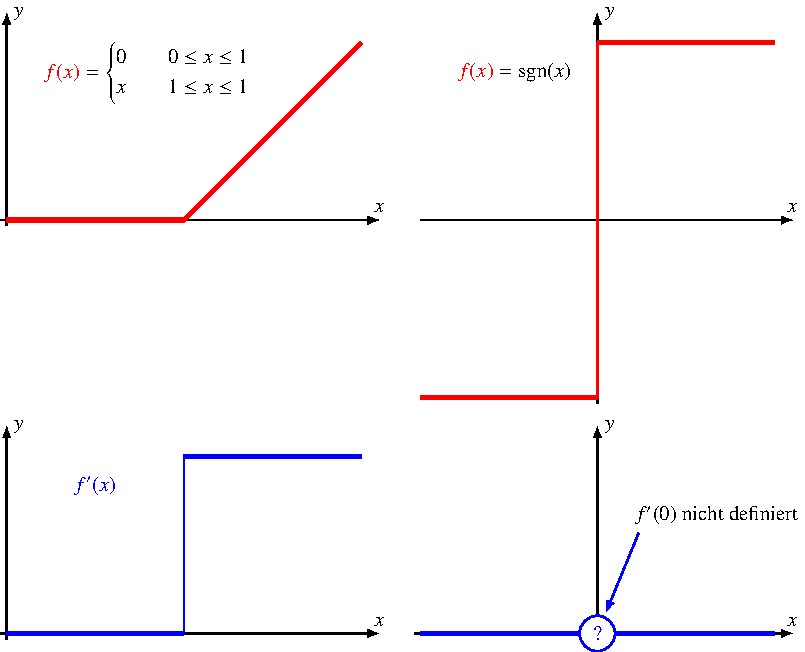
\includegraphics{chapters/010-skalarprodukt/images/schwach.pdf}
\caption{Schwache Ableitung einer nicht differenzierbaren Funktion.
Links die schwache Ableitung der Funktion von
Beispiel~\ref{buch:skalarprodukt:sobolevraum:bsp:schwachexistiert}.
Für die Signum-Funktion von
Beispiel~\ref{buch:skalarprodukt:sobolevraum:bsp:schwachexistiertnicht}
existiert die schwache Ableitung nicht, sie lässt für den Punkt $0$
nicht definieren.
\label{buch:skalarprodukt:sobolevraum:fig:schwach}}
\end{figure}
%
Die in Abbildung~\ref{buch:skalarprodukt:sobolevraum:fig:schwach} links
dargestellte Funktion
\[
f\colon (0,1) \to \mathbb{R}
:
x \mapsto
\begin{cases}
x&\qquad\text{für $0<x<1$}\\
1&\qquad\text{für $1\le x<2$}
\end{cases}
\]
ist stetig und integrierbar, aber sie ist an der Stelle $x=1$ nicht
differenzierbar.
Wir suchen die schwache Ableitung $v$ von $f$.

In einer Umgebung eines Punktes $x>1$ können wir Testfunktionen $\varphi$
so wählen, dass ihr Träger vollständig im Inneren des Intervals $(1,2)$
enthalten ist.
Mit diesen Testfunktionen können wir so rechnen, wie wenn $f$ die konstante
Funktion $1$ ist.
Das bedeutet für das Skalarprodukt
\[
\langle f,\varphi'\rangle
=
\int_1^2 \varphi'(x)\,dx
=
[\varphi(x)]_0^1 = 0.
\]
Das Skalarprodukt mit jeder beliebigen Testfunktion ist $0$, wir
müssen also $v(x)=0$ wählen.

Für $x$ im Teilinterval $(0,1)$ können wir die Testfunktionen so wählen,
dass der Träger vollständig im Inneren  von $(0,1)$ enthalten ist und
somit $f$ als die beliebig oft stetig differenzierbare Funktion $x$
behandelt werden darf.
Für das Skalarprodukt folgt dann
\[
-\langle f,\varphi'\rangle
=
-\int_0^1 f(x)\,\varphi'(x)\,dx
=
-\int_0^1 x\varphi'(x)\,dx
=
-[x\varphi(x)]_0^1 +\int_0^1 \varphi(x)\,dx
=
\langle 1,\varphi(x)\rangle,
\]
in diesem Teil des Intervals muss die schwache Ableitung den Wert $1$ 
haben.

Wir haben somit gefunden, dass die schwache Ableitung von $f$ die
Funktion
\[
v(x) = \begin{cases}
1&\qquad\text{für $0\le x<1$}
\\
0&\qquad\text{für $1< x<2$}
\end{cases}
\]
ist.
Wir kontrollieren dies, indem wir das Skalarprodukt für beliebige 
Testfunktionen $\varphi$ nachrechnen:
\begin{align*}
\langle v,\varphi\rangle
&=
\int_0^2 v(x)\,\varphi(x)\,dx
=
\int_0^1 1\,\varphi(x)\,dx
+
\int_1^2 0\,\varphi(x)\,dx.
\intertext{Jedes dieser Integrale kann man partiell integrieren:}
&=
[x\varphi(x)]_0^1 - \int_0^1 x\varphi'(x)\,dx
+
[1\varphi(x)]_1^2 - \int_1^2 1\varphi'(x)\,dx
\\
&=
\varphi(1) + \varphi(2) - \varphi(1) - \int_0^2 f(x)\,\varphi'(x)\,dx.
\intertext{Da $2$ ein Randpunkt ist, ist $\varphi(2)=0$, so dass sich}
&=-\langle f,\varphi'\rangle.
\end{align*}
ergibt.
Die Funktion $v$ ist also die schwache Ableitung von $f$.
\end{beispiel}

Eine Funktion in $W^{1,2}(\Omega)$ hat eine schwache Ableitung,
wie das Beispiel gezeigt hat, muss die Ableitung keine stetige
Funktion sein.
Ausserdem ist jede andere Funktion, die sich von der schwachen
Ableitung auf einer Menge vom Mass 0 unterscheidet, genauso eine
schwache Ableitung.
Trotzdem kann eine Funktion mit einer schwachen Ableitung nicht
beliebig ``wild'' sein, wie das folgende Beispiel zeigt.

\begin{beispiel}
\label{buch:skalarprodukt:sobolevraum:bsp:schwachexistiertnicht}
Die Signum-Funktion
\[
f\colon (-1,1) = \operatorname{sgn}(x) =
\begin{cases}
         - 1&\qquad\text{für $-1<x<0$}\\
\phantom{-}0&\qquad\text{für $x=0$}\\
\phantom{-}1&\qquad\text{für $0<x<1$}
\end{cases}
\]
ist nicht stetig (Abbildung~\ref{buch:skalarprodukt:sobolevraum:fig:schwach}).
$f$ ist fast überall konstant, in beiden Teilintervallen $(-1,0)$ und
$(0,1)$ ist die einzige mögliche schwache Ableitung von $f$ die
Nullfunktion.
Trotzdem kann $0$ nicht die schwache Ableitung von $f$ sein.
Wir wählen eine Testfunktion $\varphi$, die im Punkt $x=0$ von
Null verschieden ist.
Wäre $v$ eine schwache Ableitung von $f$, dann müsste
\begin{align*}
\langle v,\varphi\rangle
&=
-\langle f,\varphi'\rangle
=
-\int_{-1}^1 f(x) \varphi'(x)\,dx
\\
&=
-\int_{-1}^0 (-1)\cdot \varphi'(x)\,dx
-\int_{0}^1 1\cdot \varphi'(x)\,dx
=
\int_{-1}^0 \varphi'(x)\,dx
-
\int_{0}^1 \varphi'(x)\,dx
\\
&=
[\varphi(x)]_{-1}^0
-
[\varphi(x)]_{0}^1
=
\varphi(0)-\varphi(-1)
-
\varphi(1)+\varphi(0)
\\
&=
2\varphi(0)
\ne 0.
\end{align*}
Andererseits ist die Nullfunktion der einzige Kandidat für die
schwache Ableitun, für die das Skalarprodukt $\langle v,\varphi\rangle=0$
ist.
Dieser Widerspruch zeigt, dass die Funktion $f$ kein schwache
Ableitung hat.
\end{beispiel}

Die schwache Ableitung ermöglicht also mit gewissen Funktionen zu arbeiten,
die keine Ableitung im traditionellen Sinne haben.
Dank der Definition mit Hilfe eines Skalarproduktes in einem 
Hilbert-Raum darf man sich die Funktionen als Grenzwerte von
Cauchy-Folgen vorstellen.

%
% Physikalische Rechtfertigung
%
\subsection{Physikalische Rechtfertigung der schwachen Ableitung}
Die schwache Ableitung ersetzt die mit Hilfe eines Differenzenquotienten
definierte Änderungsrate durch eine Änderungsrate, die durch Vergleich
mit einer in der Umgebung eines Punktes konzentrierten Testfunktion
ermittelt wird.
Auf den ersten Blick mag das als Konzession an die Präzision der Ideen
der Analysis erscheinen, die Newton erfunden hat, um die Physik auf eine
neue Grundlage zu stellen.
Dabei wird aber vergessen, dass der Differenialquotient eine physikalisch
nicht erreichbare Idealisierung darstellt.
Keine Messung kann in einem Punkt im geometrischen Sinn erfolgen.
Die Bestimmung einer Position eines Massepunktes zum Beispiel erfolgt
durch Beobachtung des Lichtes, das vom Massepunkt reflektiert wird.
Doch der Massepunkt ist kein Punkt im geometrischen Sinn, er ist ausgedehnt
über ein endliches Gebiet.
Auch ist die Messung nicht instantan, es wird Licht gemessen, welches
über ein Zeitintervall vom Massepunkt reflektiert wird.
Das Messresultat entsteht also notwendigerweise als Mittelwert der
Beobachtung einer sehr grossen Zahl von Photonen, die von verschiedenen
Stellen reflektiert wurden.
Ein solcher Mittelwert ist genau das, was ein Skalarprodukt
$\langle f,\varphi\rangle$ mit einer Testfunktion ermittelt.

Die Feldgleichungen der Elektrodynamik wurden von Maxwell ausgehend
von Faradays Ideen als partielle Differentialgleichungen formuliert.
Sie verknüpfen die Werte des elektrischen Feldes $\vec{E}$ und des
magnetischen Feldes $\vec{B}$ mit der Ladungsdichte $\varrho$
und der Stromdichte $\vec{\jmath}$, die die Felder erzeugen.
Doch sowohl die Ladungsdichte wie auch die Stromdichte sind Idealisierungen.
Ladungen und Ströme sind nicht stetig über den Raum verteilt, sondern 
in Elektronen oder Atomkernen konzentriert.
Die Ladungsdichte entsteht daraus durch Messung der Ladung in einem kleine
Raumgebiet und Mittelung, was man wieder als Skalarprodukt mit einer
Testfunktion beschreiben kann.

Das elektrische Feld wird gemessen, indem die Kraft auf eine Testladung
im Feld ermittelt wird.
Ausser den prinzipiellen Einschränkungen an die Genauigkeit der
Positionsmessung wissen wir auch aus der Quantenmechanik, dass so etwas
wie die exakte Position eines Teilchens nicht gibt, wir können nur eine
Wahrscheinlichkeitsverteilung dafür bekommen.
Die Kraft äussert sich in einer Geschwindigkeitsänderung, die aber erst
messbar wird, wenn man die Beschleunigung eine gewisse Zeit lang aufrecht
erhält.
Das Messresultat ist also wieder ein Mittelwert über viele Positionen
und Zeitpunkte, oder anders ausgedrückt ein Skalarprodukt mit einer
Testfunktion.

Weitere Beispiele kann man auch in der Fluiddynamik finden.
Die Navier-Stokes-Gleichungen beschreiben die Strömung eines Mediums
unter der Annahme, dass es durch die Dichte $\varrho$ und die
Geschwindigkeit exakt beschreiben lässt.
Das Medium setzt sich aber aus einzelnen Atomen zusammen, die Dichte
ist also bereits ein Mittelwertbildung.
Bei der Geschwindigkeit wird das Problem noch deutlicher.
Auch die Strömungsgeschwindigkeit eines Gases ist der Mittelwert der
Strömungsgeschwindigkeit der Teilchen. 
Die Geschwindigkeit einzelner Teilchen ist dabei meistens sehr viel
grösser, nämlich im Bereich der Schallgeschwindigkeit, und äussert sich
in der Temperatur des Gases, also der mittleren kinetischen Energie.
Es ist nicht sinnvoll, von der Temperatur eines einzelnen Atoms zu
sprechen.

Alle diese Beispiele zeigen, dass die Ableitung als Änderungsrate, die
mit einem Differenzenquotienten bestimmt werden kann, eine Idealisierung
ist.
Wir können dies sogar etwas formeller zeigen.
Sei $x(t)$ die Koordinate eines Massepunktes zur Zeit $t$.
Die Messung kann nicht instantan erfolgen, im besten Fall ist die
gemessene Position ein Integral der Form
\[
\hat{x}(t)
=
\int_{-\infty}^\infty x(\tau) \varphi(\tau - t)\,d\tau.
\]
Darin ist $\varphi$ eine Testfunktion mit Träger in der Nähe von $0$.
Schreiben wir $T_t\varphi(\tau) = \varphi(\tau -t)$, dann können wir
das Messresultat auch als Skalarprodukt
$\hat{x}(t)=\langle x,T_t\varphi\rangle$
schreiben.
Die Messung mit der gleichen Aparatur einen Moment $\Delta t$ später ergibt
\[
\hat{x}(t+\Delta t)
=
\int_{-\infty}^\infty x(\tau) \varphi(\tau-t-\Delta t)\,dt
=
\langle x, T_{t+\Delta t}\varphi\rangle.
\]
Die Geschwindigkeit als Differenzenquotient ist
\begin{equation}
\frac{
\hat{x}(t+\Delta t)-\hat{x}(t)
}{\Delta t}
=
\frac{
\langle f,T_{t+\Delta t}\varphi\rangle
-
\langle f,T_{t}\varphi\rangle
}{
\Delta t
}
=
\left\langle
f,\frac{T_{t+\Delta t}\varphi - \varphi}{\Delta t}
\right\rangle
\label{buch:skalarprodukt:sobolevlraum:eqn:geschwindigkeit}
\end{equation}
Die Funktion $(T_{t+\Delta t}\varphi-T_t\varphi)/\Delta t$ ist eine 
beliebig oft stetig differenzierbare Funktion, die im Grenzwert
$\Delta t\to 0$ gegen
\[
\frac{
\varphi(\tau - t - \Delta t)
-
\varphi(\tau - t)
}{
\Delta t
}
=
-
\frac{
\varphi(\tau - t + \delta) - \varphi(\tau - t)
}{
\delta
}
\to 
-
\varphi'(\tau - t)
\quad
\text{für $\delta = - \Delta \to 0$}
\]
konvergiert.
Der Differenzenquotient
\eqref{buch:skalarprodukt:sobolevlraum:eqn:geschwindigkeit}
konvergiert daher gegen
\[
\lim_{\Delta t\to 0}
\frac{
\hat{x}(t+\Delta t)-\hat{x}(t)
}{\Delta t}
=
\left\langle
x,
\lim_{\Delta t\to 0}
\frac{T_{t+\Delta t}\varphi-T_t\varphi}{\Delta t}
\right\rangle
=
\langle f,-\varphi'\rangle
=
-
\langle f, \varphi'\rangle.
\]
Dieses einfache Modell einer ``unscharfen'' Messung führt also automatisch
auf das Konzept der schwachen Ableitung.








%\uebungsabschnitt
%\aufgabetoplevel{chapters/010-potenzen/uebungsaufgaben}
%\begin{uebungsaufgaben}
%\uebungsaufgabe{101}
%\uebungsaufgabe{102}
%\uebungsaufgabe{103}
%\uebungsaufgabe{104}
%\end{uebungsaufgaben}
%\endgroup


%
% chapter.tex -- Skalarprodukt
%
% (c) 2021 Prof Dr Andreas Müller, Hochschule Rapperswil
%
% !TeX spellcheck = de_CH
\chapter{Skalarprodukte
\label{buch:chapter:skalarprodukte}}
\kopflinks{Skalarprodukte}

%
% 1-definition.tex
%
% (c) 2023 Prof Dr Andreas Müller, OST Ostschweizer Fachhochschule
%
\section{Definition
\label{buch:opertoren:section:definition}}
\kopfrechts{Definition}


%
% 2-cauchyschwarz.tex
%
% (c) 2022 Prof Dr Andreas Müller, OST Ostschweizer Fachhochschule
%
\section{Ungleichungen
\label{buch:skalarprodukte:section:cauchyschwarz}}
\kopfrechts{Cauchy-Schwarz-Ungleichung}
In der Vektorgeometrie wird gelehrt, dass die Länge eines Vektors $u$
durch die Norm $\|u\|$ wiedergegeben wird und dass die geometrische
Intuition dazu passt.
Dazu gehört vor allem, dass die Dreiecksungleichung erfüllt ist,
dass also für drei Punkt $A$, $B$ und $C$
\begin{equation}
\overline{AB} \le \overline{AC} + \overline{BC}
\label{skalarprodukt:ungleichungen:eqn:dreieck}
\end{equation}
gilt.
In Vektorform bedeutet dies, dass
\[
\| b-a\|
\le
\| c-a\| + \|b-c\|.
\]
Schreibt man $u=c-a$ und $v=b-c$, dann ist $u+v=b-a$ und somit
\begin{equation}
\| u+v\| \le \|u\| + \|v\|.
\label{skalarprodukt:cauchyschwarz:eqn:dreieck0}
\end{equation}
Dies ist die Dreiecksungleichung in
Vektorform~\eqref{skalarprodukt:cauchyschwarz:eqn:dreieck0}.
Ziel dieses Abschnitts ist zu zeigen, dass jedes reelle oder
komplexe Skalarprodukt diese und weitere Eigenschaften automatisch
mitbringt.

%
% Cauchy-Schwarz-Ungleichung
%
\subsection{Cauchy-Schwarz-Ungleichung}
Sei also $\langle\;\,,\;\rangle$ ein reelles oder komplexes Skalarprodukt
auf dem Vektorraum $V$,
insbesondere ist $\langle v,v\rangle\ge 0$ für beliebige Vektoren $v\in V$.
Für zwei Vektoren $x,y\in V$ und $t\in \mathbb{R}$  gilt daher
\begin{align}
0
&\le
\| x+ty\|^2
=
\langle x+ty,x+ty\rangle
=
\langle x,x\rangle
+
t\langle x,y\rangle
+
t\langle y,x\rangle
+
t^2
\langle y,y\rangle.
\label{skalarprodukt:cauchyschwarz:eqn:quadrat}
\end{align}
Für ein reelles Skalarprodukt ist $\langle x,y\rangle=\langle y,x\rangle$
und damit
\begin{align}
0
&\le
\|x\|^2 + 2t\langle x,y\rangle + t^2 \|y\|^2.
\label{buch:skalarprodukt:cauchyschwarz:eqn:cspoly}
\end{align}
Dies ist ein quadratisches Polynom in der Variablen $t$, dessen Minimum
nicht negativ sein darf.

%
% Minimum eines quadratischen Polynoms
%
\subsubsection{Minimum eines quadratischen Polyoms}
Ein beliebiges quadratisches Polynom
\[
p(t)=at^2+bt+c
\]
kann durch
quadratisches Ergänzen in die Form
\[
p(t)
=
a\biggl(t+\frac{b}{2a}\biggr)^2 -\frac{b^2}{4a}+c
\]
gebracht werden.
Daraus kann man ablesen, dass das Minimum an der Stelle
\[
t_0
=
-\frac{b}{2a}
\]
angenommen wird und den Wert 
\begin{equation}
p(t_0)
=
c-\frac{b^2}{4a}
\end{equation}
hat.
Die gleiche Lösung kann natürlich auch durch Bestimmung des Minimums
von $p(t)$ mit Hilfe der Bedingung $p'(t_0)=0$ gefunden werden.

%
% Cauchy-Schwarz-Ungleichung für einen reellen Vektorraum
%
\subsubsection{Cauchy-Schwarz-Ungleichung für einen reellen Vektorraum}
Für~\eqref{buch:skalarprodukt:cauchyschwarz:eqn:cspoly}
ist
\[
a=\|y\|^2,\quad
b=2\langle x,y\rangle
\quad\text{und}\quad
c=\|x\|^2.
\]
Daher folgt aus~\eqref{buch:skalarprodukt:cauchyschwarz:eqn:cspoly}
\[
0
\le
\|x\|^2 - \frac{\langle x,y\rangle^2}{\|y\|^2}
\qquad\Rightarrow\qquad
\langle x,y\rangle^2 \le \|x\|^2\, \|y\|^2
\qquad\Rightarrow\qquad
|\langle x,y\rangle| \le \|x\|\, \|y\|.
\]
Dies ist die Cauchy-Schwarz-Ungleichung für das Skalarprodukt
$\langle \;\,,\;\rangle$.

\begin{satz}[Cauchy-Schwarz]
\label{buch:skalarprodukt:cauchy-schwarz:satz:reell}
Ein reelles Skalarprodukt $\langle\;\,,\;\rangle$ auf dem reellen Vektorraum
$V$ erfüllt die Cauchy-Schwarz-Ungleichung
\[
|\langle x, y\rangle| \le \|x\|\,\|y\|
\]
für $x,y\in V$.
\end{satz}

%
% Cauchy-Schwarz-Ungleichung für einen komplexen Vektorraum
%
\subsubsection{Cauchy-Schwarz-Ungleichung für einen komplexen Vektorraum}
Für ein komplexes Skalarprodukt ist das Produkt $\langle x,y\rangle$
nicht mehr unbedingt reell und kann damit nicht mehr direkt mit den
Normen $\|x\|^2u$ und $\|y\|^2$ vergleichen.
Wir ersetzen daher $t$ durch
$t\langle y,x\rangle=t\overline{\langle x,y\rangle}$
und erhalten 
\begin{align*}
0
\le
\|x+t\langle y,x\rangle y\|^2
&=
\langle x,x\rangle
+t\langle y,x\rangle \langle x,y\rangle
+t\overline{\langle y,x\rangle}\langle y,x\rangle
+t^2\langle y,y\rangle
\\
&=
\|x\|^2
+
t
2|\langle x,y\rangle|^2
+
t^2 |\langle x,y\rangle|^2
\|y\|^2.
\end{align*}
Dies ist wieder ein quadratisches Polynom, diesmal mit den Koeffizienten
\[
a= |\langle x,y\rangle|^2 \|y\|^2,
\quad
b= 2|\langle x,y\rangle|^2
\quad\text{und}\quad
c= \|x\|^2.
\]
Das Minimum dieses Polynoms ist nach
\[
0
\le
c-\frac{b^2}{4a}
=
\|x\|^2 - \frac{|\langle x,y\rangle|^4}{|\langle x,y\rangle|^2\,\|y\|^2}
=
\|x\|^2 - \frac{|\langle x,y\rangle|^2}{\|y\|^2}
\quad\Rightarrow\quad
|\langle x,y\rangle|^2 \le \|x\|^2\,\|y\|^2
\quad\Rightarrow\quad
|\langle x,y\rangle \le \|x\|\,\|y\|.
\]
Dies ist die Cauchy-Schwarz-Ungleichung für einen komplexen Vektorraum.

\begin{satz}[Cauchy-Satz]
\label{buch:skalarprodukt:cauchy-schwarz:satz:komplex}
Ein komplexes Skalarprodukt $\langle\;\,,\;\rangle$ auf dem komplexen Vektorraum
$V$ erfüllt die Cauchy-Schwarz-Ungleichung
\[
|\langle x, y\rangle| \le \|x\|\,\|y\|
\]
für $x,y\in V$.
\end{satz}

Man beachte, dass die
Sätze~\ref{buch:skalarprodukt:cauchy-schwarz:satz:reell}
und
\ref{buch:skalarprodukt:cauchy-schwarz:satz:komplex}
nur die Axiome eines Skalarproduktes verwenden.
Sie gelten also
ganz unabhängig von der konkreten Definition des Skalarproduktes,
solange die Eigenschaften eines Skalarproduktes gegeben sind.

\begin{beispiel}
Die sesquilineare Funktion
\[
\langle x,y\rangle
=
\sum_{i=1}^n\overline{x}_i y_i
\]
für Vektoren $x,y\in\mathbb{C}^n$ ist positiv definit, denn
\[
\langle x,x\rangle
=
\sum_{i=1}^n \overline{x}_i x_i = \sum_{i=1}^n |x_i|^2 > 0
\]
für $x\ne 0$.
Nach Satz~\ref{buch:skalarprodukt:cauchy-schwarz:satz:komplex}
gilt daher
\[
\biggl|
\sum_{i=1}^n \overline{x}_i y_i
\biggr|
\le
\sqrt{\sum_{i=1}^n |x_i|^2} \sqrt{\sum_{i=1}^n |y_i|^2}
\quad\text{oder auch}\quad
\biggl|
\sum_{i=1}^n x_i y_i
\biggr|
\le
\sqrt{\sum_{i=1}^n |x_i|^2} \sqrt{\sum_{i=1}^n |y_i|^2}
\]
für beliebige Vektoren $x,y\in\mathbb{C}^n$.
\end{beispiel}

\begin{beispiel}
Die sesquilineare Funktion
\[
\langle f,g\rangle
=
\int_a^b \overline{f(x)} g(x)\,dx
\]
für komplexwertige, stetige Funktion auf dem Intervall $[a,b]$
ist positiv definit, denn
\[
\langle f,f\rangle
=
\int_a^b \overline{f(x)} f(x)\,dx
=
\int_a^b |f(x)|^2\,dx
\ge 0
\]
für $f\ne 0$.
Nach Satz~\ref{buch:skalarprodukt:cauchy-schwarz:satz:komplex}
gilt daher
\begin{align*}
\biggl|\int_a^b \overline{f(x)}g(x)\,dx\biggr|
&\le
\sqrt{\int_a^b |f(x)|^2\,dx}
\sqrt{\int_a^b |g(x)|^2\,dx}
\intertext{oder auch}
\biggl|\int_a^b f(x) g(x)\,dx\biggr|
&\le
\sqrt{\int_a^b |f(x)|^2\,dx}
\sqrt{\int_a^b |g(x)|^2\,dx}
\end{align*}
für beliebige komplexwertige stetige Funktionen $f,g$ auf dem
Intervall $[a,b]$.
\end{beispiel}

%
% Dreiecksungleichung
%
\subsection{Dreiecksungleichung}
Die Intuition einer Längenmessung basiert auf der
Dreiecksungleichung~\eqref{skalarprodukt:ungleichungen:eqn:dreieck}.
Sie ist gleichbedeutend mit der
Vektorform~\eqref{skalarprodukt:cauchyschwarz:eqn:dreieck0}
der Ungleichung.

Die Cauchy-Schwarz-Ungleichung ermöglicht nun, diese Ungleichung
nachzurechnen.
Die Norm von $\|x+y\|^2$ ist
\[
\|x+y\|^2
=
\langle x+y,x+y\rangle
=
\langle x,x\rangle
+
\langle x,y\rangle
+
\langle y,x\rangle
+
\langle y,y\rangle
=
\|x\|^2 + 2\operatorname{Re}\langle x,y\rangle + \|y\|^2.
\]
Den mittleren Term kann man mit der Cauchy-Schwarz-Ungleichung
umformen:
\begin{align*}
\|x\|^2 + 2\operatorname{Re}\langle x,y\rangle + \|y\|^2.
&\le
\|x\|^2 + 2|\operatorname{Re}\langle x,y\rangle| + \|y\|^2.
\\
&\le
\|x\|^2 + 2|\langle x,y\rangle| + \|y\|^2.
\\
&\le
\|x\|^2 + 2\|x\|\,\|y\| + \|y\|^2
=
(\|x\| + \|y\|)^2.
\end{align*}
Durch Ziehen der Wurzel folgt
\[
\|x+y\| \le \|x\| + \|y\|.
\]
Damit ist der folgende Satz bewiesen.

\begin{satz}[Dreiecksungleichung]
Für die Norm zu einem beliebigen Skalarprodukt auf dem reellen
oder komplexen Vektorraum $V$ gilt die Dreiecksungleichung
\[
\|x+y\| \le \|x\| + \|y\|
\]
für $x,y\in V$.
\end{satz}

%
% Normen
%
\subsection{Normen
\label{skalarprodukt:cauchyschwarz:subsection:norm}}
Das Skalarprodukt ist nicht die einzige Möglichkeit, eine Norm auf
einem Vektorraum zu definieren.
Zum Beispiel kann man auf $\mathbb{C}^n$ die sogenannte $l^1$-Norm
definieren.

\begin{definition}
Die Funktion
\[
\|x\|_1
=
\sum_{i=1}^n |x_i|
\]
für $x\in\mathbb{C}^n$ heisst die {\em $l^1$-Norm} auf $\mathbb{C}^n$.
\end{definition}

Die Funktion $\|\cdot\|_1$ ist eine Norm im Sinne der folgenden Definition.

\begin{definition}
Eine Funktion $\|\cdot\| \colon V\to\mathbb{R}$ auf einem reellen
oder komplexen Vektorraum $V$ heisst eine {\em Norm}, wenn Sie die
folgenden Bedingungen erfüllt
\begin{enumerate}
\item
$\|\lambda x\| = |\lambda|\, \|x\|$ für $x\in V$ und $\lambda\in \Bbbk$
\item
Für alle Vektoren $x\in V$ mit $x\ne 0$ gilt $\|x\|>0$.
\item
Dreiecksungleichung: $\|x+y\| \le \|x\| + \|y\|$ für alle $x,y\in V$
\end{enumerate}
\end{definition}

Es ist klar, dass die $l^1$-Norm die Bedingungen~1 und 2 erfüllt.
Aber auch die Bedingung~3 kann man leicht  nachprüfen:
\[
\|x+y\|_1
=
\sum_{i=1}^n |(x+y)_i|
=
\sum_{i=1}^n |x_i+y_i|
\le
\sum_{i=1}^n(|x_i|+|y_i|)
=
\sum_{i=1}^n|x_i|
+
\sum_{i=1}^n|y_i|
=
\|x\|_1 + \|y\|_1,
\]
wozu wir nur die Dreiecksungleichung $|a+b|\le |a| + |b|$ für reelle 
oder komplexe Zahlen $a,b$ benötigen.

\begin{beispiel}
Die Funktion
\[
\|x\|_\infty = \sup_{1\le i\le n} |x_i|
\]
ist eine Norm auf $\mathbb{C}^n$.
\end{beispiel}

Auch in diesem Fall sind die Bedingungen~1 und 2 ganz offensichtlich erfüllt.
Für die Dreiecksungleichung rechnen
\begin{align*}
\|x+y\|_\infty
&=
\sup_{1\le i\le n} |x_i+y_i|
\le
\sup_{1\le i\le n} (|x_i|+|y_i|)
\le
\sup_{1\le i\le n} |x_i|+\sup_{1\le i\le n}|y_i|
=
\|x\|_\infty + \|y\|_\infty.
\end{align*}
Somit ist $\|\cdot\|_\infty$ eine Norm auf $\mathbb{C}^n$.

%
% Polaridentität
%
\subsection{Polaridentität}
Die durch das Skalarprodukt definierte Norm
\( \|x\|^2=\langle x,x\rangle \)
ist nach Abschnitt~\ref{skalarprodukt:cauchyschwarz:subsection:norm}
ein Spezialfall einer Norm.
Ist es möglich, für eine Norm, die von einem Skalarprodukt herkommt,
das Skalarprodukt wieder zu rekonstruieren?

%
% Reelles Skalarprodukt aus der Norm
%
\subsubsection{Reelles Skalarprodukt aus der Norm}
Die Antwort gibt der folgende Satz.

\begin{satz}[Polaridentität]
\label{skalarprodukt:cauchyschwarz:satz:polarformel}
Ist $\|\cdot\|$ die Norm zu einem Skalarprodukt auf dem reellen Vektorraum
$V$, dann kann das Skalarprodukt zweier Vektoren $x,y\in V$ mittels
der sogenannten {\em Polaridentität}
\index{Polaridentität}%
\begin{equation}
\langle x, y\rangle
=
\frac12\bigl(
\|x+y\|^2 - \|x\|^2 - \|y\|^2 
\bigr)
\label{skalarprodukt:cauchyschwarz:eqn:polar}
\end{equation}
berechnet werden.
\end{satz}

\begin{proof}[Beweis]
Die Gleichung
\begin{align*}
\|x+y\|^2
&=
\langle x+y,x+y\rangle
=
\|x\|^2 + 2\langle x,y\rangle + \|y\|^2 
\end{align*}
kann nach $\langle x,y\rangle$ aufgelöst werden und ergibt
die behauptete Formel~\eqref{skalarprodukt:cauchyschwarz:eqn:polar}.
\end{proof}

% 
% Parallelogrammgleichung
%
\subsubsection{Parallelogrammgleichung}
\begin{figure}
\centering
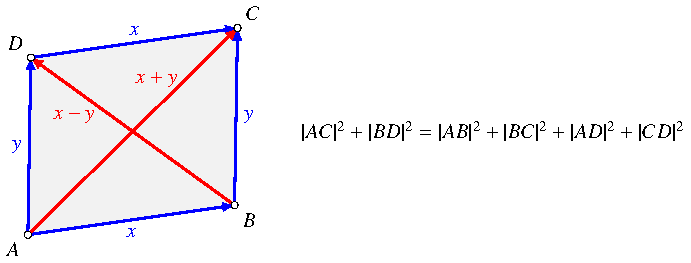
\includegraphics{chapters/010-skalarprodukt/images/parallelogramm.pdf}
\caption{Parallelogrammregel für eine Norm, die aus einem Skalarprodukt
entsteht.
\label{skalarprodukt:cauchyschwarz:fig:parallelogramm}}
\end{figure}
Die Polaridentitäten können auch noch in einer anderen Form geschrieben
werden.
Dazu berechnet man zusätzlich die Norm von $x-y$:
\begin{align*}
\|x+y\|^2
&=
\|x\|^2 + \|y\|^2 + 2\langle x, y\rangle
\\
\|x-y\|^2
&=
\|x\|^2 + \|y\|^2 - 2\langle x, y\rangle
\\
\|x+y\|^2 +\|x-y\|^2
&=
2\|x\|^2 + 2\|y\|^2
\end{align*}

\begin{satz}
\label{skalarprodukt:cauchyschwarz:satz:parallelgramm}
Für eine Norm, die von einem reellen Skalarprodukt herkommt, gilt die
Parallelogrammformel
\begin{equation}
\|x+y\|^2 +\|x-y\|^2
=
2\|x\|^2 + 2\|y\|^2.
\label{skalarprodukt:cauchyschwarz:eqn:parallelgramm}
\end{equation}
(Abbildung~\ref{skalarprodukt:cauchyschwarz:fig:parallelogramm})
\end{satz}

Das Skalarprodukt kann man damit auf verschiedene Weise aus der
Norm gewinnen:
\begin{equation}
\begin{aligned}
\langle x, y\rangle
&=
{\textstyle\frac12}\bigl( \|x\|^2 + \|y\|^2 - \|x+y\|^2 \bigr)
\\
&=
{\textstyle\frac12}\bigl(
\|x+y\|^2
-
\|x\|^2 
-
\|y\|^2
\bigr)
\\
&=
{\textstyle\frac14}\bigl(
\|x+y\|^2 - \|x-y\|^2
\bigr).
\end{aligned}
\label{skalarprodukt:cauchyschwarz:eqn:realteil}
\end{equation}
Nur die letzte Formel ist noch nicht gut begründet.
Man kann aber sofort nachrechnen, dass 
\begin{align*}
\|x+y\|^2&=\|x\|^2+2\langle x,y\rangle+\|y\|^2\\
\|x-y\|^2&=\|x\|^2-2\langle x,y\rangle+\|y\|^2
\intertext{die Differenz}
\|x+y\|^2 - \|x-y\|^2 &= 4\langle x,y\rangle
\qquad
\Rightarrow
\qquad
\langle x,y\rangle
=
\frac14\bigl(\|x+y\|^2 - \|x-y\|^2\bigr)
\end{align*}
haben.

%
% Komplexes Parallelogramm aus der Norm
%
\subsubsection{Komplexe Skalarprodukt}
Das Resultat von Satz~\ref{skalarprodukt:cauchyschwarz:satz:polarformel}
gilt in abgeänderter Form auch für komplexe Skalarprodukte.
Da das Skalarprodukt auch einen nichtverschwindenen Imaginärteil haben
kann, wird eine zusätzliche Gleichung zur Berechnung des Imaginärteils
nötig.
Eine solche kann gewonnen werden, indem zusätzlich die Normen
$\|x+iy\|^2$ und $\|x-iy\|^2$ berechnet werden.
Dazu ist zu beachten, dass
\[
\langle x,y\rangle
-
\langle y,x\rangle
=
\langle x,y\rangle
-
\overline{
\langle x,y\rangle
}
=
2i\operatorname{Im}\langle x,y\rangle
\]
Damit erhält man
\begin{align*}
\|x+iy\|^2 &= \|x\|^2 + i\langle x,y\rangle - i\langle y,x\rangle + \|y\|^2 
           = \|x\|^2 + 2\operatorname{Im}\langle x,y\rangle + \|y\|^2 \\
\|x-iy\|^2 &= \|x\|^2 - i\langle x,y\rangle + i\langle y,x\rangle + \|y\|^2 
           = \|x\|^2 - 2\operatorname{Im}\langle x,y\rangle + \|y\|^2.
\end{align*}
Damit kann man nach dem Imaginärteil des Skalarproduktes auflösen und
die Formeln
finden, die den Formeln
\eqref{skalarprodukt:cauchyschwarz:eqn:realteil}
für das reelle Skalarprodukt entsprechen.
\eqref{skalarprodukt:cauchyschwarz:eqn:realteil}
Formeln bleiben gültig als Formeln für den Realteil des Skalarproduktes.
Damit haben wir den folgenden Satz gefunden.

\begin{satz}[Polaridentitäten für ein komplexes Skalarprodukt]
Ist $\|\cdot\|$ die Norm, die aus dem komplexen Skalarprodukt
$\langle\;\,,\;\rangle$ auf einem Vektorraum $V$ gewonnen wurde,
dann können Real- und Imaginärteil mit den Formeln
\begin{align*}
\operatorname{Re}\langle x,y\rangle
&=
{\textstyle\frac12}\bigl(
\|x+y\|^2 - \|x\|^2 -\|y\|^2
\bigr)
\\
&=
{\textstyle\frac12}\bigl(
\|x\|^2 +\|y\|^2 - \|x+y\|^2
\bigr)
\\
&=
{\textstyle\frac14}\bigl(
\|x+y\|^2 - \|x-y\|^2
\bigr),
\\
\operatorname{Im}\langle x,y\rangle
&=
{\textstyle\frac12}\bigl(
\|x+iy\|^2-\|x\|^2-\|y\|^2
\bigr)
\\
&=
{\textstyle\frac12}\bigl(
\|x\|^2+\|y\|^2-\|x-iy\|^2
\bigr)
\\
&=
{\textstyle\frac14}\bigl(
\|x+iy\|^2
-
\|x-iy\|^2
\bigr)
\end{align*}
für beliebige Vektoren $x,y\in V$
allein aus Werten der Norm berechnet werden.
\end{satz}


%
% 3-funktionenraeume.tex
%
% (c) 2022 Prof Dr Andreas Müller, OST Ostschweizer Fachhochschule
%
\section{Funktionenräume
\label{buch:skalarprodukt:section:funktionenraeume}}
\kopfrechts{Funktionenräume}
Ziel der harmonischen Analysis ist die effiziente Approximation einer
grossen Klasse von Funktionen.
Als approximierende Funktionen kommen stetige Funktionen, Polynome,
trigonometrische Polynome oder eine ähnlich, einfach konstruierbare
Funktionenfamilie in Frage.
Es gilt zunächst herauszufinden, was ``Approximation'' genau heissen
soll und von welchen Funktionen man überhaupt erwarten kann, dass sie
approximiert werden können.

%
% Stetige Funktionen
%
\subsection{Stetige Funktionen
\label{buch:skalarprodukt:subsection:stetige-funktionen}}
Der frühe intuitive Funktionsbegriff ging oft von der Vorstellung einer
in einem Strich gezeichneten Kurve aus, wie man sie von den Graphen
der Polynome oder der trigonometrischen Funktionen her kennt.
In moderner Sprechweise sind dies die stetigen Funktionen.

\begin{definition}
Eine Funktion $f\colon I\to\mathbb{R}$ mit $I\subset \mathbb{R}$
heisst stetig in einem Punkt $x_0\in I$, wenn für jedes $\varepsilon>0$
ein $\delta>0$ existiert derart, dass $f(x)-f(x_0)|<\delta$ sobald
$|x-x_0|<\varepsilon$.
\end{definition}

Nur die Eigenschaft, eine Abstandsmessung zu besitzen, wird vom
Definitionsbereich $I\subset \mathbb{R}$ verlangt.
Der Stetigkeitsbegriff kann daher verallgemeinert werden auf den
Begriff des metrischen Raumes.

\begin{definition}
Eine {\em Metrik} auf einer Menge $X$ ist eine Funktion
\index{Metrik}%
$d\colon X\times X\to \mathbb{R}$
mit den folgenden Eigenschaften
\begin{enumerate}
\item
Positiv definit: $d(x,y)\ge 0$ und $d(x,y)$ genau dann, wenn $x=y$.
\item
Symmetrie: \(d(x,y)=d(y,x)\)
\item
Dreiecksungleichung: \( d(x,y) \le d(x,z) + d(z,y) \).
\end{enumerate}
Ein {\em metrischer Raum} ist ein Menge $X$ mit einer Metrik.
\index{matrischer Raum}%
\end{definition}

In einem metrischen Raum ist der Begriff des Grenzwertes übertragbar.
Mit dem Begriff des Grenzwertes lässt sich auch der Begriff der
Stetigkeit verallgemeinern.

\begin{definition}
Ist $x_n\in X$ eine Folge von Punkten in einem metrischen Raum $X$,
dann heisst $x$ der Grenzwert der Folge $x_n$, wenn es für jedes
$\varepsilon>0$ ein $N>0$ gibt derhart, dass
$d(x_n,x)\le \varepsilon$ für alle $n>N$.
Eine Funktion $f\colon X\to Y$ zwischen metrischen Räumen heisst
stetig im Punkt $x\in X$, wenn für jede Folge $x_n\in X$ mit
Grenzwert $x$ auch die Folge $y_n=f(x_n)\in Y$ konvergiert und
den Grenzwert $y=f(x)$ hat.
\end{definition}

Teilmengen von $\mathbb{R}$ oder $\mathbb{R}^n$ tragen natürlich
die Struktur eines metrischen Raumes mit der Abstandsmessung in 
$\mathbb{R}^n$ als Metrik
\[
d(x,y) = \sqrt{(x_1-y_1)^2 + \ldots + (x_n-y_n)^2} = \|x-y\|.
\]
Die Eigenschaften einer Metrik wurden bereits in Abschnitt
\ref{buch:skalarprodukte:section:cauchyschwarz} nachgewiesen.

Der Begriff des Grenzwertes klärt, was mit der Approximation von $x$
durch eine Folge $x_n$ gemeint ist.
Wenn man darauf aufbauend die Konvergenz einer Folge von Funktionen
gegen eine Grenzfunktion definieren will, braucht man einen Abstansbegriff
zwischen Funktionen.
Ein erster Versuch könnte sein, als Abstand zwischen zwei Funktionen
$f$ und $g$ die Funktion
\[
d(f,g) = |f(x_0) - g(x_0)|.
\]
Die Menge der Funktionen wird dadurch jedoch nicht zu einem metrischen
Raum.
Zwar gilt sicher die Symmetrie und Dreiecksungleichung, und auch 
$d(f,g)\ge 0$ für beliebige Funktionen.
Aber wenn $d(f,g)=0$ ist, heisst das nur, dass $f$ und $g$ im Punkt
$x_0$ den gleichen Wert haben.
Ausser in trivialen Fällen wird es Funktionen geben, die zwar im Punkt
$x_0$ übereinstimmen, sich aber in mindestens einem anderen Punkt
unterscheiden.

%
% Normierte Räume
%
\subsubsection{Normierte Räume}
Die stetigen Funktionen bilden aber keine strukturlose Menge, sie
bilden einen Vektorraum: die Summe von stetigen Funktionen ist ebenfalls
stetig, multiplizieren einer stetigen Funktion mit einem Skalar führt
nicht aus der Menge der stetigen Funktionen heraus.
Die für den Grenzwertbegriff von Funktionen verwendete Abstandsmessung 
sollte der Vektorraumstruktur ebenfalls Rechnung tragen.

\begin{definition}
\label{buch:skalaprodukt:funktionenraume:def:norm}
Sei $V$ ein Vektorraum über $\mathbb{R}$, dann heisst eine Funktion
\( \|\;\cdot\;\| \colon V \to \mathbb{R}\) eine {\em Norm}, wenn gilt
\index{Norm}
\begin{enumerate}
\item
Definit: $ \|x\| = 0 \Rightarrow x=0$
\item
Homogeneität: $ \| \lambda x \| = |\lambda| \cdot \|x\|$
\item
Dreiecksungleichung: $\|x+y\| \le \|x\| + \|y\|$
\end{enumerate}
Ein {\em normierter Raum} ist ein Vektorraum $V$ mit einer Norm.
\end{definition}

%
% Vollständigkeit
%
\subsubsection{Vollständigkeit}
In den rationalen Zahlen hat nicht jede Folge einen Grenzwert.
Die Zahl $\sqrt{2}$ lässt sich beliebig genau durch rationale Zahlen
approximieren, sie ist aber nicht in $\mathbb{Q}$.
Ähnlich lässt sich die Funktion $x\mapsto \sqrt{x}$ beliebig genau 
durch Polyome approximieren, sie ist aber selbst kein Poylnome

\begin{definition}
Ein Folge $x_n\in X$ in einem metrischen Raum heisst {\em Cauchy-Folge},
wenn es für jedes $\varepsilon>0$ ein $N>0$ gibt derart, dass 
$|x_n-x_m|<\varepsilon$ wenn $n,m>N$ ist.
\end{definition}

Cauchy-Folgen sind also Folgen, die sich für genügend grossen Index
kaum mehr ändern und für die man daher Konvergenz erwarten würde.

\begin{definition}
Ein normierter Raum heisst {\em vollständig} oder ein Banach-Raum,
wenn jede Cauchy-Folge einen Grenzwert hat.
\end{definition}

Die rationalen Zahlen $\mathbb{Q}$ bilden keinen vollständigen
metrischen Raum, aber die reellen Zahlen $\mathbb{R}$ enthalten
alle Grenzwerte von Cauchy-Folgen, $\mathbb{R}$ ist eine vollständiger
metrischer Raum.
Die Menge der Polynome, betrachtet als Teilmenge der Menge der
stetigen Funktionen $[0,1]\to\mathbb{R}$ ist nicht vollständig,
da es eine Folge $f_n(x)$ von Approximationsfunktionen der Funktion
$x\mapsto \sqrt{x}$ gibt.
Als Cauchy-Folge konvergiert sie zwar gegen eine stetige Funktion,
aber die Grenzfunktion ist nicht mehr im Raum der Polynome.

Das Ziel der folgenden Kapitel ist also, zu geeignet interessanten
Funktionenfamilien ``gute'' Normen zu finden derart, dass Cauchy-Folgen
konvergieren gegen Funktionen, die immer noch ausreichend viele
nützliche Eigenschaften haben.
Im besten Fall konvergieren stetige Funktionen gegen stetige Funktionen,
es wird sich aber zeigen, dass diese Anforderung zu streng ist.

%
% Norm fpr stetige Funktionen
%
\subsection{Norm für stetige Funktionen
\label{buch:skalarprodukt:subsection:normfuerstetigefunktionen}}
Damit man von Konvergenz von Folgen stetiger Funktionen sprechen kann,
brauchen wir jetzt also eine Norm für stetige Funktionen.

\begin{definition}
Sei $X$ ein metrischer Raum und
\[
C(X)
=
C_{\mathbb{R}}(X)
=
\{
f\colon X \to\mathbb{R}\mid
\text{$f$ ist stetig}
\}
\]
der Vektorraum der stetigen Funktion auf $X$.
Die Norm von $C(X)$ ist definiert als
\[
\|f\| = \sup_{x\in X} |f(x)|.
\]
Sie heisst die {\em Supremum-Norm}.
\end{definition}

Wir prüfen nach, dass die Supremum-Norm tatsächlich eine Norm ist.
Dazu sind die definierenden Eigenschaften nachzurechnen:
\begin{enumerate}
\item Definit: 
\[
0
=
\|f\|
=
\sup_{x\in X} |f(x)|
\quad\Rightarrow\quad
f(x)=0 \;\forall x\in X
\quad\Rightarrow\quad
f\in C(X).
\]
\item Homogeneität:
\[
\|\lambda f\|
=
\sup_{x\in X} |\lambda f(x)|
=
|\lambda| \sup_{x\in X} |f(x)|
=
|\lambda| \cdot \|f\|.
\]
\item
Dreiecksungleichung:
\[
\|f+g\|
=
\sup_{x\in X}|f(x)+g(x)|
\le
\sup_{x\in X}(|f(x)|+|g(x)|)
\le
\sup_{x\in X}|f(x)|+\sup_{x\in X}|g(x)|
=
\|f\| + \|g\|.
\]
\end{enumerate}

Eine Cauchy-Folge $f_n$ von Funktionen $X\to \mathbb{R}$ hat die
Eigenschaft, dass für jedes $\varepsilon >0$ ein $N>0$ existiert,
derart dass $\|f_n-f_m\|<\varepsilon$ ist.
Da die Norm der maximale Unterschied von Funktionswerten ist,
folgt dass für eine Cauchy-Folge in $C(X)$ die Folge $f_n(x)$ eine
Cauchy-Folge in $\mathbb{R}$ ist und damit einen Grenzwert in $\mathbb{R}$
hat.
Die Funktion $f(x) = \lim_{n\to\infty}f_n(x)$ ist die Grenzfunktion.
Die Konvergenz bezüglich der Norm besagt, dass für jedes $\varepsilon>0$
es ein $N>0$ gibt derart, dass
\[
\varepsilon 
>
\|f_n-f\|
\ge 
|f_n(x)-f(x)|
\]
ist für alle $n>N$ und unabhängig von $x\in X$.
Die Konvergenz bezüglich der $\|\;\cdot\;\|$-Norm ist also die wohlbekannte
gleichmässige Konvergenz.
Es kann gezeigt werden, dass die Grenzfunktion wieder stetig ist.

\begin{satz}
Der Raum der stetigen Funktion $C(X)$ mit der Supremumg-Norm ist
ein Banach-Raum.
\end{satz}

%
% Skalarprodukt
%
\subsection{Skalarprodukt
\label{buch:skalarprodukt:subsection:skalarprodukt}}
\begin{figure}
\centering
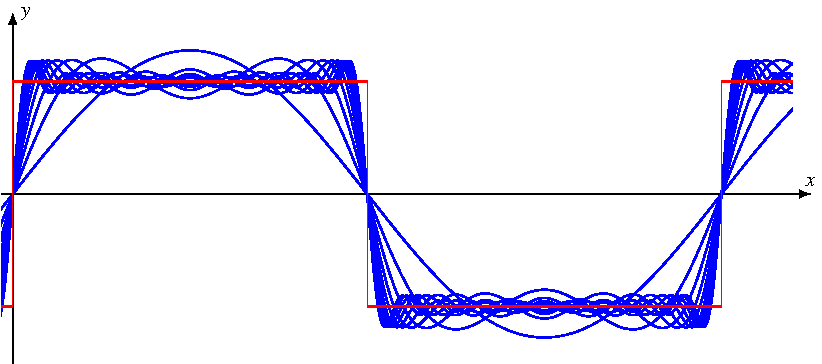
\includegraphics{chapters/010-skalarprodukt/images/fourierrechteck.pdf}
\caption{Approximation der Rechteckfunktion (rot) durch eine Folge
von Partialsummen der Fourier-Reihe.
\label{buch:skalarprodukt:fig:fourierrechteck}}
\end{figure}%
Die Supremum-Norm auf dem Raum der stetigen Funktionen hat den
Begriff der gleichmässig konvergenten Funktionenfolgen ergeben.
Cauchy-Folgen von stetigen Funktionen in der Supremum-Norm konvergieren
wieder gegen eine stetige Funktione.
Ist eine Funktion nicht stetig, lässt Sie sich im Sinne der Supremum-Norm
nicht durch stetige Funktionen approximieren.
Andererseits hat Fourier gezeigt, wie man technische wichtige Funktionen
wie die Rechteckfunktion durch trigonometrische Polynome
\begin{equation}
f_n(x)
=
\frac{4}{\pi} \sum_{k=0}^n \frac{\sin kx}{k}
=
\frac{4}{\pi} \biggl(
\sin x
+
\frac{\sin 3x}{3}
+
\frac{\sin 5x}{5}
+
\frac{\sin 7x}{7}
+
\ldots
\biggr)
\label{buch:skalarprodukt:eqn:rechteckreihe}
\end{equation}
approximieren kann.
Diese sind alle stetig und kommen der Rechteckfunktion in jedem Punkt,
in dem die Funktion stetig ist, beliebig nahe.
An den Stellen $x = n\pi$ hat die Grenzfunktion eine Sprungstelle,
die approximierenden Funktionen haben dort immer Abstand $1$
(siehe Abbildung~\ref{buch:skalarprodukt:fig:fourierrechteck}).
Die Folge ist also keine Cauchy-Folge und sie konvergiert nicht im
Sinne der Supremum-Norm.
Für solche Anwendungen muss eine besser geeignete Norm gefunden werden,
in der die Folge konvergiert.

%
% Skalarprodukt von Funktion
%
\subsubsection{Die $L^1$-Norm einer Funktion}
Die Supremum-Norm sieht nur den grössten Wert, die Konvergenz der Folge
\eqref{buch:skalarprodukt:eqn:rechteckreihe} ist aber nicht gleichmässig,
die maximale Abweichung ist immer $1$.
Gesucht ist eine Norm, die für die Folge
\eqref{buch:skalarprodukt:eqn:rechteckreihe} 
nur im Mittel eine Abweichung feststellt.
Für die Berechnung des Mittelwerts kann das Integral verwendet werden:

\begin{definition}
\label{buch:skalaprodukt:definition:l1norm}
Für eine stetige Funktion $X\to\mathbb{R}$, für die $x\mapsto |f(x)|$
integrierbar ist, heisst
\begin{equation}
\|f\|_1 = \int_X |f(x)|\,dx
\label{buch:skalarprodukt:eqn:l1norm}
\end{equation}
die {\em $L^1$-Norm} der Funktion $f$.
\end{definition}

Die $L^1$-Norm ist tatsächlich eine Norm, wir verifizieren die
definierenden Eigenschaften einer Norm.
\begin{enumerate}
\item
Definit: Sei $f$ eine stetige Funktion mit $\|f\|_1=0$
Wäre $f\ne 0$, dann gäbe es einen Punkt $x_0\in X$ mit $f(x_0) \ne 0$.
Da $f$ stetig ist, ist $f|(x)| > \frac12|f(x_0)|$ für $x$ in einer
$\delta$-Umgebung von $x_0$.
Dann folgt für die $L^1$-Norm
\begin{align*}
\|f\|_1
=
\int_X |f(x)|\,dx
\ge
\frac12 |f(x_0)| \cdot \delta 
> 0.
\end{align*}
Dies widerspricht der Annahme, dass $\|f\|_1=0$ ist, also muss $f=0$ sein.
\item
Homogeneität folgt durch direkte Rechnung
\[
\|\lambda f\|_1
=
\int_X |\lambda f(x)|\,dx
=
|\lambda|
\int_X |f(x)|\,dx
=
|\lambda| \cdot \|f\|.
\]
\item
Die Dreiecksungleichung folgt aus
\[
\|f+g\|_1
=
\int_X |f(x) + g(x)|\,dx
\le
\int_X |f(x)| + |g(x)|\,dx
=
\int_X |f(x)| + \int_X |g(x)|\,dx
=
\|f\|_1 + \|g\|_1.
\]
\end{enumerate}

Die $L^1$-Norm ist etwas ``schwächer'' als die Supremum-Norm im
folgenden Sinne.
Eine in der Supremum-Norm konvergente Funktionenfolge auf einem
kompakten Definitionsbereich $X$ ist auch in der $L^1$-Norm konvergent.
Zur Unterscheidung der verschiedenen Normen werden wir in Zukunft die
Supremum-Norm manchmal auch als $\|f\|_{\infty} = \|f\|$ schreiben.

\begin{satz}
Ist $X$ eine kompakte Teilmenge von $\mathbb{R}$ und $f_n$ eine
in der Supremum-Norm konvergente Folge stetiger Funktionen $f_n$,
dann ist $f_n$ auch in der $L^1$-Norm konvergent.
\end{satz}

\begin{proof}
Konvergenz in der Supremum-Norm bedeutet, dass für jedes $\varepsilon>0$
ein $N>0$ existiert derart, dass $|f_n(x)-f(x)|<\varepsilon$ für alle
$x\in X$ und alle $n>N$.
Für die $L^1$-Norm gilt dann
\begin{align*}
\|f_n-f\|_1
&=
\int_X |f_n(x) - f(x)|\,dx
\le
\int_X \varepsilon \,dx
=
\varepsilon \int_X \,dx
=
\varepsilon \operatorname{vol}(X).
\end{align*}
Da für einen kompakten Definitionsbereich $\operatorname{vol}(X)<\infty$
gilt, bedeutet dies, dass die $\|f_n-f\|_1\to 0$, dass also $f_n$ in
der $L^1$-Norm konvergiert.
\end{proof}

\begin{beispiel}
Die Folge $f_n(x)$ von \eqref{buch:skalarprodukt:fig:fourierrechteck}
konvergiert tatsächlich in der $L^1$-Norm auf dem Intervall $[0,2\pi]$.
Zwar ist $f_n$ nicht gleichmässig konvergent, aber fast.
Man kann zeigen, dass für jedes $\delta>0$, die Funktionen
$f_n(x)$ in Punkten $x$, die weiter als $\delta$ von den
Punkten $k\pi$ mit $k\in\mathbb{Z}$, gleichmässig konvergieren.
Innerhalb einer $\delta$-Umgebung der Vielfachen von $\pi$ ist die
$f_n(x)-f(x)$ beschränkt.
Die genaue Schranke ist nicht wichtig, wir nennen sie $M$ und bekommen
\[
|f_n(x)-f(x)|
\le M
\quad\forall x\in X.
\]
Ausserhalb einer kleinen Umgebung konvergiert die Folge gleichmässig,
zu jedem $\varepsilon>0$ gibt es also ein $N>0$ derart, dass
\[
|f_n(x)-f(x)|<\varepsilon
\]
für $x$ weiter als $\delta$ von $k\pi$ entfernt.
Für die $L^1$-Norm folgt dann
\begin{align*}
\|f_n-f\|_1
&=
\int_0^{2\pi} |f_n(x)-f(x)|\,dx
\\
&=
\int_0^\delta |f_n(x)-f(x)|\,dx
+
\int_\delta^{\pi-\delta} |f_n(x)-f(x)|\,dx
+
\int_{\pi-\delta}^{\pi+\delta} |f_n(x)-f(x)|\,dx
\\
&\qquad
+
\int_{\pi+\delta}^{2\pi-\delta} |f_n(x)-f(x)|\,dx
+
\int_{2\pi-\delta}^{2\pi} |f_n(x)-f(x)|\,dx
\\
&\le
\delta M
+
\varepsilon (\pi -2\delta)
+
2\delta M
+
\varepsilon (\pi -2\delta)
+
\delta M
\le
4\delta M + 2\pi\varepsilon
\end{align*}
für $n>N$.
Dadurch, dass man $\delta$ und $\varepsilon$ klein macht, kann man
also immer ein $N$ finden, so dass $\|f_n-f\|_1$ beliebig klein wird
für $n>N$.
Damit ist gezeigt, dass die Folge $f_n$ in der $L^1$-Norm konvergiert.
\end{beispiel}

Das Beispiel zeigt, dass die $L^1$-Norm eine schwäre Form der Konvergenz
ist, die eine erweiterte Klasse von Funktionen durch stetige Funktionen
zu approximieren erlaubt.

%
% Das $L^2$-Skalarprodukt
%
\subsubsection{Das $L^2$-Skalarprodukt}
Die $L^1$-Norm ist weniger strikt als die Supremum-Norm, aber sie ist
immer noch recht weit von der Intuition entfernt, die wir von der
Entfernungsmessung in der Geometrie haben, die von einem Skalarprodukt
herrühren.
Das Beispiel~\ref{buch:skalarprodukt:cauchyschwarz:beispiel:skalarprodukt}
weist den Weg, mit dem wir eine Norm für stetige Funktionen gewinnen
können, die von einem Skalarprodukt herkommt.

\begin{definition}
\label{buch:skalarprodukt:funktionraeume:definition:skalarprodukt}
Das {\em Skalarprodukt} stetiger Funktionen auf $X\subset \mathbb{R}$
ist definiert durch
\begin{equation}
\langle f,g\rangle
=
\int_X f(x)g(x)\,dx.
\label{buch:skalarprodukt:funktionraeume:eqn:skalarprodukt}
\end{equation}
\end{definition}

Es genügt nachzurechnen, dass $\langle f,g\rangle$ die Eigenschaften
eines Skalarproduktes hat, dann folgt die Dreiecksungleichung automatisch.
Zunächst ist klar,
dass~\eqref{buch:skalarprodukt:funktionraeume:eqn:skalarprodukt}
bilinear ist:
\begin{align*}
\langle \lambda f_1+\mu f_2,g\rangle
=
\int_X (\lambda f_1(x) + \mu f_2(x)) g(x)\,dx
&=
\lambda\int_Xf_1(x)g(x)\,dx + \mu\int_X f_2(x)g(x)\,dx
\\
&=
\lambda\langle f_1,g\rangle + \mu\langle f_2,g\rangle
\\
\langle f,\lambda g_1+\mu g_2\rangle
=
\int_X f(x)(\lambda g_1(x)+\mu g_2(x))\,dx
&=
\lambda\int_X f(x)g_1(x)\,dx + \mu\int_X f(x)g_2(x)\,dx
\\
&=
\lambda\langle f,g_1\rangle + \mu\langle f,g_2\rangle.
\end{align*}
Die Bilinearform ist aber auch positiv definit: Für eine stetige
Funktion $f(x)$ gilt
\[
\langle f,f\rangle
=
\int_X f(x)^2\,dx \ge 0.
\]
Da auch $f(x)^2$ eine stetige Funktion ist,
verschwindet das Integral genau dann, wenn $f(x)=0\;\forall x\in X$ ist.

Die zum Skalarprodukt gehörige Norm 
\[
\|f\|_2
=
\int_X |f(x)|^2\,dx
\]
heisst auch die {\em $L^2$-Norm}.

%
% Nicht kompakte Definitionsbereiche
%
\subsubsection{Nicht kompakter Definitionsbereich}
Für stetige Funktionen auf einem kompakten Definitionsbereich scheinen
die drei Normen $\|\;\cdot\;\|_\infty$, $\|\;\cdot\;\|_1$ und
$\|\;\cdot\;\|_2$ zu den gleichen Konvergenzbegriffen zu führen.
In diesem Abschnitt soll gezeigt werden, dass dies für nicht kompakte
Definitionsbereiche nicht mehr gilt.
Nicht einmal die Menge der Funktionen, die eine endliche Norm haben,
ist gleich.

\begin{beispiel}
Auf dem Definitionsbereich $X=(0,1]$ hat die Funktion
$f(x)=\log x$ endliche $L^1$-Norm aber unendliche Supremum-Norm.

\medskip
\noindent
Wegen $\lim_{x\to 0+}\log x = -\infty$ folgt $\|\log\|=\infty$.
Für die $L^1$-Norm folgt mit der Substitution $y=\log x$ und
$dy = dx/x$ oder $dx = e^y\,dy$
\begin{align*}
\|\log\|_1
&=
\int_0^1|\log x|\,dx
=
-\int_0^1\log x\,dx
=
-\int_{-\infty}^0 e^y\,dy
=
-\biggl[ e^y \biggr]_0^{-\infty}
=
1.
\end{align*}
Insbesondere ist die $L^1$-Norm beschränkt.
\end{beispiel}

\begin{beispiel}
Auf dem Definitionsbereich $X=[1,\infty)$ hat die Funktion
$f(x)=1/x$ endliche $L^2$-Norm aber unendlich $L^1$-Norm.

\medskip
\noindent
Die Integrale für die Normen ergeben:
\begin{align*}
\|f\|_1
&=
\int_1^\infty \frac{1}{x}\,dx
&
\|f\|_2^2
&=
\int_1^\infty \frac{1}{x^2}\,dx
\\
&=\biggl[\log x\biggr]_1^\infty
&
&=\biggl[-\frac{2}{x}\biggr]_1^\infty
\\
&=\infty
&
&=2.
\end{align*}
Insbesondere ist die $L^1$-Norm unbeschränkt, die $L^2$-Norm dagegen
beschränkt.
\end{beispiel}

\begin{satz}
Eine stetige Funktion auf einem beschränkten Definitionsbereich $X$
mit endlicher $L^2$-Norm hat auch endliche $L^1$-Norm.
\end{satz}

\begin{proof}[Beweis]
Aus der Cauchy-Schwarz-Ungleichung folgt
\begin{align*}
\int_X |f(x)|\,dx
&=
\langle |f|, 1\rangle
\le
\|f\|_2\cdot \|1\|_2.
\end{align*}
Nach Voraussetzung an die Funktion $f$ ist der erste Faktor beschränkt,
der zweite Faktor ist $\operatorname{vol}(X)$ und nach Voraussetzung
auch beschränkt.
\end{proof}

Die Beispiele zeigen, dass die Existenz der Normen selbst für stetige
Funktionen für nicht kompakten Definitionsbereich nicht garantiert ist.
Die Erweiterung auf nicht stetige Funktionen kann muss daher beschränkt
werden auf eine Klasse von Funktionen, für die die entsprechende Norm
existiert.
Das kann bedeuten, dass nicht alle stetigen Funktionen in Betracht 
kommen und dass neue Funktionen, die nicht stetig sind, als
Grenzwerte auftreten können.

%
% Grenzen des Riemann-Integrals
%
\subsection{Grenzen des Riemann-Integrals}
In den vorangegangenen Rechnungen sind wir immer vom Riemann-Integral
ausgegangen, welches man im Analysisunterricht als erstes kennenlernt.
Man zeigt dort, dass es für stetige Funktionen existiert und für
gleichmässig konvergente Folgen von Funktionen der Grenzwert des
Integrals mit dem Integral des Grenzwertes übereinstimmt:
\[
\int_X \lim_{n\to\infty} f_n(x)\,dx
=
\lim_{n\to\infty}
\int_X f_n(x)\,dx
\]
Der vorangegangene Abschnitt hat gezeigt, dass wir die Klasse der
Funktionen ausdehnen müssen auf Funktionen, die nicht stetig sind,
für die aber immer noch die $L^1$- oder die $L^2$-Norm existiert.
Hier zeigen sich die Schwächen des Riemann-Integrals.
In diesem Abschnitt soll an Beispielen gezeigt werden, was schief
gehen kann, und wie das Problem gelöst werden kann.

%
% Abzählbar viele Stetigkeitsstellen
%
\subsubsection{Abzählbar viele Unstetigkeitsstellen}
Wir konstruieren eine Funktionenfolge von Riemann-integrierbaren 
Funktionen, die alle das Integral $0$ haben, deren Grenzfunktion
aber nicht mehr Riemann-integrierbar ist.

Die rationalen Zahlen im Intervall $[0,1]$ sind abzählbar, d.~h.~es
gibt eine Folge $n\mapsto q_n\in[0,1]\cap\mathbb{Q}$, in der jede
rationale Zahl im Intervall vorkommt.
Aus der Folge $q_n$ konstruieren wir jetzt die Folge von Funktionen
\[
f_n(x)
=
\begin{cases} 
1&\qquad\text{$x$ ist einer der Werte $q_1,q_2,\ldots,q_n$}\\
0&\qquad\text{sonst}.
\end{cases}
\]
Die Funktion $f_n(x)$ ist also an genau $n$ Stellen von $0$ erschieden
und hat dort den Wert $1$.
Das Riemann-Integral ``sieht'' endlich viele Sprungstellen nicht,
die Funktionen $f_n$ sind also alle Riemann-integrierbar und haben
das Integral
\[
\int_0^1 f_n(x)\,dx=0.
\]
Insbesondere ist auch
\[
\lim_{n\to\infty}\int_0^1 f_n(x)\,dx = 0.
\]
Andererseits ist die Grenzfunktion
\begin{equation}
f(x)
=
\begin{cases}
1&\qquad\text{$x\in[0,1]\cap\mathbb{Q}$ ist rational}\\
0&\qquad\text{sonst, $x$ ist irrational.}
\end{cases}
\label{buch:skalarprodukt:funktionenraeume:eqn:ratfunk}
\end{equation}
Das Riemann-Integral der Funktion $f(x)$ existiert nicht.
Dazu müsste man ja für eine Unterteilung $0=x_0<x_1<\dots x_n=1$
die Riemann-Summen
\[
\overline{I}
=
\sum_{k=0}^{n-1}
(x_{k+1}-x_k) \sup_{x_k\le \xi \le x_{k+1}} f(\xi)
\qquad\text{und}\qquad
\underline{I}
=
\sum_{k=0}^{n-1}
(x_{k+1}-x_k) \inf_{x_k\le \xi \le x_{k+1}} f(\xi)
\]
berechnen, und sie müssten bei Verfeinerung der Unterteilung
gegeneinander konvergieren.
Aufgrund der Konstruktion der Funktion $f(x)$ ist aber
\[
\sup_{x_k\le \xi \le x_{k+1}} f(\xi) = 1
\qquad\text{und}\qquad
\inf_{x_k\le \xi \le x_{k+1}} f(\xi) = 0,
\]
sodass
$\overline{I}=1$ und $\underline{I}=0$ ist, ganz unabhängig von
der Unterteilung.

Der Riemannsche Integralbegriff muss also für die Zwecke der Approxmation
mit der $L^1$ oder $L^2$-Norm erweitert werden, so dass er sinnvoll mit
abzählbar vielen Unstetigkeitsstellen umgehenn kann.
Insbesondere sollte er als Integral der Funktion $f(x)$ 
von \eqref{buch:skalarprodukt:funktionenraeume:eqn:ratfunk}
den Wert $0$ liefern.

%
% Masse
%
\subsubsection{Masstheorie}
Gesucht wird also ein Integral, das für eine grössere Klasse von
Funktionen definiert ist und welches sich bezüglich Grenzwerten
besser verhält als das Riemann-Integral.
Das Integral ist nur dann nützlich, wenn es für viele Funktionen
die gleichen Werte ergibt.

Die einfachsten Funktionen, die wir integrieren wollen, sind die
{\em Indikatorfunktionen}, Funktionen, die durch eine Teilmenge
\index{Indikatorfunktion}
$A\subset X$ definiert sind durch
\[
1_A(x)
=
\begin{cases}
1&\qquad\text{für $x\in A$}\\
0&\qquad\text{sonst}.
\end{cases}
\]
Für ein Intervall der Länge $\lambda(A)$ ist
\[
\int_X 1_A(x)\,dx = \lambda(A).
\]
Für Mengen, die sich aus vielen Intervallen zusammensetzen, erwarten wir
die Summenformel
\[
A=\bigcup_{k=1}^\infty A_k,
\quad
A_k\cap A_j = \emptyset\;\forall k\ne j
\qquad\Rightarrow\qquad
\lambda(A) = \sum_{k=1}^\infty \lambda(A_k).
\]
Ausserdem sollte für eine Teilmenge $A\subset B$ der Inhalt der
Differenz $\lambda(A\setminus B)=\lambda(A)-\lambda(B)$ sein.

So entsteht eine Klasse von Mengen, denen sinnvoll ein Inhalt 
zugeordnet werden kann.
Solche Mengen heissen {\em messbar}.
Dazu gehören alle Intervalle, aber auch alle Differenzen und
abzählbaren Vereinigungen von Intervallen und messbaren Mengen
sind wieder messbar.
Die Klasse der messbaren Mengen ist also sehr gross.
Es braucht natürlich noch einiges an Arbeit, um zu zeigen, dass
eine widerspruchsfreie Definition der Funktion $\lambda(A)$
tatsächlich möglich ist, die jeder messbaren Menge einen
Inhalt zuordnet.
Eine solche Funktion heisst ein {\em Mass}, das aus der Intervalllänge
konstruierte Mass heisst auch das Lebesgue-Mass nach Henri Léon Lebesgue..
\index{Lebesgue-Mass}%
\index{Mass}%

Von besonderem Interesse sind Mengen, deren Inhalt $0$ ist.

\begin{definition}
\label{buch:skalarprodukt:funktionenraeume:definition:nullmenge}
Eine Nullmenge bezüglich des Masses $\lambda$ ist eine messbare
Menge $A$ mit Mass $\lambda(A)=0$.
\index{Nullmenge}
\end{definition}

Der Riemannsche Integralbegriff lässt bei der Bestimmung des Masses
nur endlich viele Intervalle zu. 
Die Menge $Q$ der rationalen Zahlen im Intervall $[0,1]$ ist abzählbar
unendlich.
In jeder beliebigen Umgebung einer reellen Zahl in $[0,1]$ findet man
rationale Zahlen in $Q$, eine Überdeckung der Menge der rationalen
Zahlen mit endlich vielen Intervallen enthält daher immer auch alle
reellen Zahlen, mit der möglichen Ausnahme von endlich vielen Zahlen.
Der Inhalt, den der Riemannsche Integralbegriff der Menge $Q$ zuordnen
muss, ist daher $1$.

Der neue Massbegriff erlaubt, die Menge mit abzählbar vielen messbaren
Mengen zu überdecken.
Sei $q_k$ eine Folge, die alle rationalen Zahlen in $Q$ durchläuft.
Zu jedem $k$ konstruieren wir das Intervall
\[
A_k = (q_k-\varepsilon2^{-k},q_k+\varepsilon2^{-k})
\]
mit Inhalt $\lambda(A_k) = 2\varepsilon2^{-k}$.
Es ist klar, dass die Intervalle $A_k$ die ganze Menge $Q$ überdecken,
also
\[
Q\subset \bigcup_{k=1}^\infty A_k.
\]
Der Inhalt der Menge $Q$ ist daher
\[
\lambda(Q)
\le
\sum_{k=1}^\infty \lambda(A_k)
=
\sum_{k=1}^\infty 2\varepsilon 2^{-k}
=
2\varepsilon
\sum_{k=1}^\infty 2^{-k}
=
2\varepsilon.
\]
Da $\varepsilon$ beliebig klein gewählt werden kann, folgt, dass
$\lambda(Q)=0$ sein muss.
Aus diesem Beispiel lässt sich erahnen, dass der Lebesguesche Massbegriff
mit Grenzwerten besser umgehen kann als der aus dem Riemannschen Integral
abgeleitete.

%
% Lebesgue-Integral
%
\subsubsection{Lebesgue-Integral}
Aus der Konstruktion eines Masses $\lambda$ kann jetzt die Konstruktion
eines Integrals an die Hand genommen werden.
Dazu werden Funktionen durch Stufenfunktionen approximiert, die
von der Form
\[
f(x) = \sum_{k=1}^\infty a_k 1_{A_k}(x)
\]
sind, wobei $A_k$ messbare Mengen sind.
Für solche Funktionen ist die naheliegende Definition des Integrals
\[
\int_X f(x)\,d\lambda(x)
=
\sum_{k=1}^\infty a_k \lambda(A_k).
\]
Der wesentliche Unterschied zur Riemannsschen Konstruktion ist,
dass nicht nur Intervalle zulässig sind sondern beliebige messbare Mengen.
Die Berechnung des Inhalts einer messbaren Mengen beinhaltet bereits
die Möglichkeit, Grenzwerte zu bilden.
Auch hier ist viel Arbeit notwendig um nachzuweisen, dass sich aus diesem
Ansatz ein widerspruchsfreier neuer Integralbegriff ergibt.
Das so konstruierte Integral heisst das {\em Lebesgue-Integral} und
\index{Lebesgue-Integral}%
wird zur Unterscheidung vom gewöhnlichen Riemannschen Integral und
wegen der Bedeutung des Masses $\lambda$, welches eine grosse Rolle
bei seiner Konstruktion spielt mit
\[
\int_X f(x) \,d\lambda(x)
\]
bezeichnet.

Beim Riemannschen Integral haben endliche Mengen und Mengen mit endlich
vielen Häufungspunkten Inhalt $0$.
Viele abzählbare Mengen haben dagegen positiven Inhalt.
Das Lebesguesche Mass gibt allen abzählbaren Mengen den Inhalt 0.

Unterscheiden sich zwei Funktionen $f$ und $g$ nur auf einer Nullmenge,
sagt man, sie seien {\em fast überall} gleich, geschrieben
\[
f(x) = g(x) \qquad \text{fast überall}.
\]
Zwei fast überall gleiche Funktionen haben das gleiche Integral, denn
\[
\int_X f(x)\,dx - \int_X g(x)\,dx
=
\int_X f(x)-g(x)\,dx
=
\int_X 0\,dx=0
\]
weil das Integral einer fast überall verschwindenden Funktion $0$ ist.

%
% Funktionsklassen
%
\subsubsection{Klassen von fast überall gleichen Funktionen}
Verwendet man die mit dem Lebesgque-Integral berechnete $L^1$- oder
$L^2$-Norm, dann können Funktionen nicht voneinander unterschieden werden,
die fast überall gleich sind.
Grenzwerte von Funktionenfolgen in der $L^1$- oder $L^2$-Norm sind
daher nur bis auf eine Nullmenge bestimmt.

\begin{definition}
Die Menge der Lebesgue-integrierbaren Funktionen auf dem Definitionsbereich
$X\subset\mathbb{R}$ wird mit
\[
\mathscr{L}^1(X)
=
\mathscr{L}^1_{\mathbb{R}}(X)
=
\left\{ f\colon X\to \mathbb{R}
\;\left|\;
\text{$f$ ist $\lambda$-integrierbar und $\int_X|f(x)|\,dx< \infty$}
\right.\right\}
\]
bezeichnet.
Entsprechend besteht $\mathscr{L}^2(X)$ aus den Funktionen $X\to \mathbb{R}$,
für die $|f(x)|^2$ integrierbar ist.
Sie heissen auch die {\em quadratintegrierbaren} Funktionen.
\end{definition}

Das Lebesgue-Integral kann Funktionen, die sich nur auf einer Nullmenge
verschieden sind, nicht unterscheiden. 
Daher ist es notwenig, solche Funktionen in Klassen zusammenzufassen:

\begin{definition}
Die Relation
\[
f\sim g
\qquad:\Leftrightarrow \qquad f(x) = g(x)\quad\text{fast überall}
\]
ist eine Äquivalenzrelation.
Die Menge der Äquivalenzklassen von Funktionen in $\mathscr{L}^1(X)$
bezüglich dieser Relation werden mit $L^1(X)$ bezeichnet, ebenso werden
die Äquivalenzklassen von $\mathscr{L}^2(X)$ bezüglich der Relation $\sim$
mit $L^2(X)$ bezeichnet.
\end{definition}

Mit den Funktionsklassen in $L^1(X)$ und $L^2(X)$ lässt sich genau
so rechnen, wie man es sicht gewohnt ist.
Für die Summe von Funktionen $f_1\sim f_2$ und $g_1\sim g_2$ gilt
\[
\left.
\begin{aligned}
f_1(x)&=f_2(x)&&\text{fast überall}\\
g_1(x)&=g_2(x)&&\text{fast überall}\\
\end{aligned}
\quad
\right\}
\qquad
\Rightarrow
\qquad
f_1(x)+g_1(x) = f_2(x)+g_2(x)\quad\text{fast überall},
\]
denn die Menge, auf der sich $f_1+f_2$ und $g_1+g_2$ unterscheiden
ist höchstens die Vereinigung der Mengen, auf denen sich $f_1$ und 
$f_2$ bzw.~$g_1$ und $g_2$ unterscheiden.
Die Vereinigung von Nullmengen ist aber wieder eine Nullmenge.

%
% Lebesgue-Integral
%
\subsubsection{Dominierte Konvergenz}
Die Entwicklung des Lebesgueschen Integrallbegriffs war motiviert
vom Wunsch, ein Integral zu erhalten, welches sich bezüglich
Konvergenz von Funktionenfolgen besser verhält.
Tatsächlich liefert die Theorie den folgenden zentralen Satz.

\begin{satz}[Dominierte Konvergenz]
\label{buch:skalarprodukt:satz:dominierte-konvergenz}
Sei $f_n$ eine auf dem Definitionsbereich $X$ punktweise konvergente
Folge Lebesgue-integrierbarer Funktionen mit Grenzfunktion 
\[
f(x) = \lim_{n\to \infty} f_n(x).
\]
Sei ausserdem $g$ eine Lebesgue-integrierbare Funktion mit
$|f_n(x)|<g(x)$ für alle $x\in X$.
Dann ist $f$ Lebesgue-integrierbar und es gilt
\[
\lim_{n\to\infty} \int_X f(x)\,d\lambda(x)
=
\int_X f(x)\,d\lambda(x)
\]
\end{satz}

Der Satz der dominierten Konvergenz von Lebesgue ersetzt also die
Bedingung der gleichmässigen Konvergenz, die beim Riemann-Integral
erfolgreich war, durch die viel schächere Bedingung, dass alle
Funktionen unterhalb einer gemeinsamen integrierbaren Funktion bleiben.
Dadurch wird verhindert, dass die Funktionen $f_n$ nach $\infty$
``ausbrechen'' kann und gegen eine Funktion konvergieren, die nicht
mehr integrierbar ist.


%
% Berechnung von Lebesgue-Integralen
%
\subsubsection{Berechnung von Lebesgue-Integralen}
Das Lebesque-Integral löst also die technischen Probleme, die das
Riemann-Integral manchmal bei Funktionenfolgen hat, die gegen ein
Grenzfunktion konvergieren, der man ein sinnvolles Integral im
Lebesgueschen Sinnen zuordnen kann.
Doch wie berechnet man ein Lebesgue-Integral?

Stetige Funktionen lassen sich beliebig genau durch Treppenfunktionen
approximieren.
Die Konvergenz des Lebesgue-Integrals für solche Funktionenfolgen
garantiert daher, dass das Lebesgue-Integral für stetige
Funktionen mit dem Riemann-Integral übereinstimmt.
Insbesondere braucht es keinen neuen Formalismus für die 
Berechnung von Integralen.
Auch für Funktionen, die an höchstens endlich vielen Stellen unstetig
sind, stimmt das Riemann-Integral mit dem Lebesgue-Integral überein.

Man soll sich daher das Lebesgue-Integral vor allem als eine 
Erweiterung des Integrals auf Funktionen vorstellen, die als Grenzwerte
von Folgen stetiger Funktionen im Sinne der $L^1$- oder der $L^2$-Norm
auftreten können.
Stetigkeit kann dabei verloren gehen, aber Konvergenzeigenschaften
wie die dominierte Konvergenz von
Satz~\ref{buch:skalarprodukt:satz:dominierte-konvergenz}
bleiben erhalten.




%
% 4-hilbertraum.tex
%
% (c) 2022 Prof Dr Andreas Müller, OST Ostschweizer Fachhochschule
%
\section{Hilbert-Raum
\label{buch:skalarprodukt:section:hilbertraum}}
\kopfrechts{Hilbert-Raum}
Ein Skalarprodukt stattet einen Vektorraum mit einer Norm aus.
Es ermöglicht auch, orthonormierte Vektoren zu finden.
In endlichdimensionalen Vektorräumen können so besonders nützliche
Basen konstruiert werden.
In den Funktionenräumen von
Abschnitt~\ref{buch:skalarprodukt:section:funktionenraeume},
die unendlichdimensional sind, kann der Orthonormalisierungsprozess
ohne Ende weitergeführt werden.
Im Gegensatz zu einem endlichdimensionalen Vektorraum bilden diese
orthonormierten Vektoren keine Basis, denn nicht jeder Vektor lässt
sich als Linearkombination schreiben.
Dies wird erst mit Hilfe von Reihenentwicklungen möglich, doch dazu
müssen Fragen der Konvergenz solcher Reihen geklärt werden.
Der in diesem Abschnitt eingeführte Begriff des Hilbert-Raumes tut dies.

%
% Prähilbertraum
%
\subsection{Prähilbertraum}
Die Funktionenräume, in denen wir harmonische Analysis betreiben wollen,
zeichnen sich durch das Vorhandensein eines Skalarproduktes aus.
Wir fassen diese Eigenaschaften im Begriff des Prähilbertraumes
zusammen.

\begin{definition}
Ein reeller Prähilbertraum ist ein reller Vektorraum mit einem
(reellen) Skalarprodukt.
\index{Prähilbertraum}%
Eine komplexer Prähilbertraum ist ein komplexer Vektorraum mit einem
sesquilinearen Skalarprodukt.
\end{definition}

\begin{beispiel}
Der endlichdimensionale reelle Vektorraum $\mathbb{R}^n$ ist ein
reller Prähilbertraum mit dem Skalarprodukt
\[
\langle u,v\rangle
=
\sum_{i=1}^n u_iv_i
\]
für Vektoren $u,v\in\mathbb{R}^n$.
\end{beispiel}

\begin{beispiel}
Der endlichedimensionale komplexe Vektorrau $\mathbb{C}$ ist ein
komplexer Prähilbertraum mit dem Skalarprodukt
\[
\langle u,v\rangle
=
\sum_{i=1}^n \overline{u}_iv_i
\]
für Vektoren $u,v\in\mathbb{C}^n$.
\end{beispiel}

Die Skalarprodukte in den Beispielen sind nicht die einzig möglichen
Skalarprodukte.
Alternative Skalarprodukte auf einem reellen Prähilbertraum können 
durch eine beliebige positiv definite Matrix $A$ durch
\[
\langle u,v\rangle_A
=
\sum_{i,j=1}^n u_ia_{ij}v_j
\]
definiert werden.
Wir schreiben die aus $\langle\;,\;\rangle_A$ abgeleitete Norm mit
$\normfunc_A$.
Solange unser primäres Interesse der Approximation von Funktionen gilt,
kommt es vor allem darauf an, dass die Norm, die aus dem Skalarprodukt
abgeleitet wird, zu den gleichen konvergenten Folgen führen.
Die Funktion $u\mapsto \|u\|_A$ ist stetig, sie hat daher auf der
Einheitskugel des Prähilbertraumes ein Maximum und eine Minimum,
welches wir mit $M$ bzw.~$m$ bezeichen.
Dann folgt, dass
\[
m\|u\|\le \|u\|_A\le M\|u\|
\]
für beliebige Vektoren $u\in\mathbb{R}^n$.
Daraus kann man jetzt ableiten, dass die beiden Normen $\normfunc$
und $\normfunc_A$ auf die gleichen Cauchy-Folgen und die gleichen
konvergenten Folgen führen.
Wir zeigen dies für Cauchy-Folgen:
\begin{enumerate}
\item
Sei $u_k$ eine Cauchy-Folge bezüglich der Norm $\normfunc$,
und $\varepsilon>0$.
Wir müssen zeigen, dass $u_k$ auch eine Cauchy-Folge ist bezüglich
der Norm $\normfunc_A$.
Da $u_k$ eine Cauchy-Folge bezüglich der Norm $\normfunc$ ist,
gibt es ein $N>0$ derart, dass
$\|u_k-u_l\|<\varepsilon/M$ für $k,l>N$.
Dann folgt aber
\[
\|u_k-u_l\|_A
\le
M\|u_k-u_l\|
<
M\frac{\varepsilon}{M}
=
\varepsilon
\]
für $k,l>N$.
Somit ist $u_k$ eine Cauchy-Folge bezüglich der Norm $\normfunc_A$.
\item
Ist umgekehrt  $u_k$ eine Cauchy-Folge bezüglich der Norm $\|\,\cdot\,\|_A$,
dann gibt es ein $N>0$ derart, dass $\|u_k-u_l\|_A<m\varepsilon$ ist für
$k,l>N$.
Dann folgt
\[
m\|u_k-u_l\|\le \|u_k-u_l\|_A < m\varepsilon
\qquad\Rightarrow\qquad \|u_k-u_l\|<\varepsilon
\]
für $k,l>N$, also ist $u_k$ auch eine Cauchy-Folge bezüglich der Norm
$\|\,\cdot\,\|$.
\end{enumerate}
In einem endlichdimensionalen Prähilbertraum hat die Wahl des Skalarproduktes
keinen Einfluss darauf, ob eine Folge eine Cauchy-Folge ist oder nicht.
Orthonormierte Vektoren werden natürlich im Allgemeinen nicht mehr
orthonormiert, dies ist jedoch ein Aspekt, dem wir uns erst später
zuwenden werden.

%
% Orthonormierte Vektoren
%
\subsection{Orthonormierte Vektoren in einem Prähilbertraum}
Der Gram-Schmidt-Orthogonalisierungsprozess kann auf eine beliebige
\index{Gram-Schmidt}%
linear unabhängige Menge von Vektoren in einem Prähilbertraum angewendet
werden.
Aus den linear unabhängigen Vektoren $a_1,a_2,\dots$ werden die
orthonormierten Vektoren
\begin{align*}
b_1
&=
\frac{a_1}{\|a_1\|}
\\
b_2
&=
\frac{
a_2 - \langle b_1,a_2\rangle b_1
}{
\|a_2 - \langle b_1,a_2\rangle b_1\|
}
\\
&\phantom{i}\vdots
\\
b_n
&=
\frac{\displaystyle
a_n - \sum_{k=1}^{n-1} \langle b_k,a_n\rangle b_k
}{\displaystyle
\biggl\|a_n - \sum_{k=1}^{n-1} \langle b_k,a_n\rangle b_k\biggr\|
}.
\end{align*}

In einem endlichdimensionalen Vektorraum der Dimension $n$ bricht
der Prozess ab, sobald eine orthonormierte Basis $b_1,\dots,b_n$
aus $n$ Vektoren gefunden wurde.
Jeder andere Vektor $v$ lässt sich dann als Linearkombination
\begin{equation}
v
=
\langle b_1,v\rangle b_1 + \langle b_2,v\rangle b_2 + \dots
=
\sum_{k=1}^n \langle b_1,v\rangle b_1
\label{buch:skalarprodukt:hilbertraum:synthese}
\end{equation}
schreiben.
Da die Summe auf der rechten Seite endlich ist, entstehen keine
Bedenken bezüglich Konvergenz, wie das bei einer unendlichen
Reihe der Fall wäre.

%
% Vollständigkeit
%
\subsection{Vollständigkeit}
In einem unendlichdimensionalen Prähilbertraum bricht der
Orthogonalisierungsprozess nicht ab, es gibt immer noch einen
linear unabhängigen Vektor, der nicht in dem von den bereits
gefundenen Vektoren aufgespannten Raum liegt.
Die Summe~\ref{buch:skalarprodukt:hilbertraum:synthese} wird dann
eine unendliche Summe, die nur im Sinne eines Grenzwertes der
Partialsummenfolge
\begin{equation*}
s_n = \sum_{k=1}^n \langle b_k,v\rangle b_k
\end{equation*}
ausgewertet werden kann.
Man darf zwar aufgrund der Konstruktion aus $v$ davon ausgehen,
dass $s_n$ gegen $v$ konvergiert,
aber für eine beliebige Folge von Koeffizienten $c_k$ ist nicht
garantiert, dass die Summe
\[
\sum_{k=1}^\infty c_kb_k
=
\lim_{n\to\infty} \sum_{k=1}^n c_kb_k
\]
einen Grenzwert hat.
Ein nützliche Theorie kann nur entstehen, wenn gefordert wird,
dass jede Cauchy-Folge des Prähilbertraums tatschächlich konvergiert.

\begin{definition}
Ein Prähilbertraum heisst {\em Hilbert-Raum}, wenn er vollständig ist.
\end{definition}

Endlichdimensionale Vektorräume über sind automatisch vollständig,
da gibt es also gar keinen Unterschied zwischen Prähilbertraum und
Hilbert-Raum.
Das folgende Beispiel zeigt, dass dies für unendlichdimensionale
Hilbert-Räume nicht mehr zutrifft.

\begin{beispiel}
\label{buch:skalarprodukt:hilbertraum:bsp:sinreihe}
Der Funktionenraum
\(
C_{\mathbb{R}}([-\pi,\pi])
\)
der stetigen Funktionen auf dem Intervall $[-\pi,\pi]$ wird mit
dem Skalarprodukt
\[
\langle f,g\rangle
=
\int_{-\pi}^\pi f(x)g(x)\,dx
\]
zu einem Prähilbert-Raum.
Die Summanden der Reihe~\eqref{buch:skalarprodukt:eqn:rechteckreihe} 
sind Sinus-Funktionen, von denen wir später zeigen werden, dass sie
orthogonal sind.
Seien $s_n(x)$ die Partialsummen der Reihe, also
\begin{equation}
s_n(x) = \frac{4}{\pi}\sum_{k=0}^n \frac{\sin (2k+1)x}{2k+1},
\label{buch:skalarprodukt:hilbertraum:eqn:sn}
\end{equation}
dann kann man auch die Norm $\|s_n-s_m\|$, es gilt nämlich
\begin{equation}
\|s_n-s_m\|
=
\biggl\|
\frac{4}{\pi}
\sum_{k=m}^n \frac{\sin (2k+1)x}{2k+1}
\biggr\|,
\label{buch:skalarprodukt:hilbertraum:eqn:snsm}
\end{equation}
wobei wir $n>m$ angenommen haben, was wir ohne Beschränkung der 
Allgemeinheit tun dürfen.
Die Norm eines einzeln Terms ist
\begin{align}
\|\sin rx\|^2
&=
\int_{-\pi}^\pi \sin^2 rx\,dx
=
\int_{-\pi}^\pi \frac12 - \frac{\cos rx}{2}\,dx
=
\int_{-\pi}^\pi \frac12\,dx - \int_{-\pi}^\pi \frac{\cos rx}{2}\,dx.
\notag
\intertext{Der zweite Term ist ein Integral über eine Periode des
Integranden und verschindet daher.
Der erste Term ergibt daher}
\|\sin rx\|^2
&= \pi.
\intertext{Für die Terme der Summe
\eqref{buch:skalarprodukt:hilbertraum:eqn:sn}
folgt daher}
\biggl\|
\frac{\sin{2k+1}x}{2k+1}
\biggr\|^2
&=
\frac{\pi}{(2k+1)^2}.
\notag
\intertext{Für die Differenz
\eqref{buch:skalarprodukt:hilbertraum:eqn:snsm} finden wir daher}
\|s_n-s_m\|^2
\notag
&=
\frac{16}{\pi^2}
\sum_{k=m}^m \frac{\pi}{(2k+1)^2}
=
\frac{16}{\pi}
\sum_{k=m}^m \frac{1}{(2k+1)^2}.
\label{buch:skalarprodukt:hilbertraum:eqn:bsprest}
\end{align}
Da aus dem Analysisunterricht bekannt ist, dass die Reihe $\sum_k\frac1{k^2}$
konvergiert, kann die rechte Seite von 
\eqref{buch:skalarprodukt:hilbertraum:eqn:bsprest}
beliebig klein gemacht werden, die 
Reihe~\eqref{buch:skalarprodukt:eqn:rechteckreihe} 
ist also eine Cauchy-Folge im Prähilbertraum $C_{\mathbb{R}}([-\pi,\pi])$.
Die Grenzfunktion ist die Rechteckfunktion von
Abbildung~\ref{buch:skalarprodukt:fig:fourierrechteck}, sie ist nicht
stetig.
Wir haben also eine Cauchy-Folge im Prähilbertraum 
$C_{\mathbb{R}}([-\pi,\pi])$ gefunden, die darin nicht konvergiert.
\end{beispiel}

%
% Hilbert-Basis
%
\subsection{Hilbert-Basis}
Sei jetzt $H$ ein Hilbert-Raum.
Führt man wieder die Konstruktion einer orthonormierten Basis durch,
entsteht eine Menge $\mathcal{B}=\{b_1,b_2,\dots\}$ orthonormierter
Vektoren.
In einem unendlichdimensionalen Hilbert-Raum ist $\mathcal{B}$ eine
undendliche Menge.
Die Vollständigkeit des Hilbert-Raumes garantiert, dass jede
Cauchy-Folge konvergiert, insbesondere können wir zu jedem beliebigen
Vektor $v$ die Koeffizienten $c_k=\langle b_k,v \rangle$ bestimmen
und versuchen, mit der
Summe~\eqref{buch:skalarprodukt:hilbertraum:synthese}
den Vektor zurückzugewinnen.
Vollständigkeit garantiert zwar die Konvergenz gegen einen Grenzwert
\[
v_0 = \sum_{k=1}^\infty c_k b_k,
\]
aber es gibt keine Garantie, dass $v=v_0$ ist.

\begin{beispiel}
Die Funktionen
\[
b_k(x) = \sin (2k+1)x
\qquad\text{mit}\quad
k\in \mathbb{N}
\]
wurden in Beispiel~\ref{buch:skalarprodukt:hilbertraum:bsp:sinreihe}
die Rechteckfunktion synthetisiert.
Doch reichen diese Funktionen nicht aus, um alle Funktionen auf
dem Intervall $[-\pi,\pi]$ zu synthetisieren.

Für die konstante Funktion $v(x)$ sind die Koeffizienten
\[
\langle v,b_k\rangle
=
\int_{-\pi}^\pi v(x)b_k(x)\,dx
=
\int_{-\pi}^\pi \sin (2k+1)x\,dx
=
0,
\]
die Summe
\[
v_0
=
\sum_{k=0}^\infty
c_k
b_k(x)
=
0
\]
verschwindet also, $v\ne v_0$.
\end{beispiel}

Wir berechnen das Skalarprodukt 
\[
\langle v-v_0,b_k\rangle
=
\langle v,b_k\rangle
-
\biggl\langle \sum_{l=1}^\infty c_lb_l,b_k\biggr\rangle
=
c_k - \sum_{l=1}^\infty c_l\langle b_l,b_k\rangle
=
c_k - \sum_{l=1}^\infty c_l\delta_{lk}
=
c_k-c_k=0.
\]
Der Vektor $v-v_0$ muss also orthogonal sein zu allen Vektoren
$b_k$.
Die Menge der Vektoren $b_k$ kann also vergrössert werden um einen
weiteren Vektor, der zu allen vorhandenen Vektoren orthogonal ist.

\begin{satz}
Eine Menge von orthogonalen Vektoren in einem Prähilbertraum ist linear 
unabhängig.
\end{satz}

\begin{proof}[Beweis]
Angenommen, die orthogonalen Vektoren  $a_1,\dots,a_n$ sind linear
abhängig.
Dann gibt es Zahlen $\lambda_i$, die nicht alle $=0$ sind und derart,
dass
\[
\sum_{k=1}^n \lambda_ka_k
=
\lambda_1 a_1 + \ldots + \lambda_n a_n
=
0.
\]
Das Skalarprodukt mit $a_k$ ergibt
\[
0
=
\langle a_k,\lambda_1a_1 +\ldots + \lambda_na_n\rangle
=
\lambda_1
\langle a_k,a_1\rangle
+
\ldots
+
\lambda_n
\langle a_k,a_n\rangle
=
\lambda_k \|a_k\|^2
\]
für alle $k=1,\dots,n$.
Da die Vektoren $a_k\ne 0$ sind folgt, dass $\lambda_k=0$ sein muss
für alle $k=1,\dots,n$, im Widerspruch zur Voraussetzung, dass die
$\lambda_k$ nicht alle verschwinden.
Der Widerspruch zeigt, dass die Annahme der linearen Abhängigkeit
falsch ist.
\end{proof}

In einem endlichdimensionalen Prähilbertraum findet man immer eine
orthonormierte Basis, aus der sich jeder Vektor linear kombinieren
lässt.
In einem unendlichdimensionalen Raum muss dieser Begriff etwas 
erweitert werden.

\begin{definition}
Eine {\em Hilbert-Basis} des Hilbert-Raumes $H$ ist eine Menge von orthonormalen
\index{Hilbert-Basis}%
Vektoren $b_k\in H$, $k\in \mathbb{N}$ derart, für jeden Vektor $v\in H$
die Reihe 
\[
\sum_{k\in\mathbb{N}} \langle b_k,v\rangle b_k
\]
konvergiert und die Summe $v$ hat.
\end{definition}

Auf eine Hilbert-Basis ist die Inuition anwendbar, die man von 
einer orthonormierten Basis eines endlichdimensionalen Prählibertraumes
hat.

\begin{definition}
\index{separabel}%
Ein Hilbert-Raum, der eine Hilbert-Basis besitzt, heisst {\em separabel}.
\end{definition}

Nicht separable Hilbert-Räume sind deutlich grösser.
In einem nicht separable Hilbert-Raum ist es nicht möglich, alle Vektoren
aus einer Folge von orthonormierten Vektoren linear zu kombinieren.
Dies verträgt sich nicht mit der Intuition, die in endlichdimensionalen
Vektorräumen entstanden ist.
Separabilität ist eine Art ``Endlichkeitseigenschaft''.
Man findet sie zum Beispiel bei den $L^2$-Räumen mit kompaktem
Definitionsgebiet.
Kompaktheit kann als eine topologische
Endlichkeitseigenschaft angesehen werden.
Es lassen sich aber auch nicht separable Hilbert-Räume konstruieren,
zum Beispiel sogenannte fastperiodische Funktionen.
\index{fastperiodische Funktionen}%
Für unsere Anwendungen sind nicht separable Hilbert-Räume jedoch nicht
notwendig und wir können im folgenden annehmen, dass alle Hilbert-Räume
separabel sind und somit eine Hilbert-Basis haben.

%
% Der Hilbert-Raum $l^2$
%
\subsection{Der Hilbert-Raum $l^2$}
Die abstrakte Definition eines separablen Hilbert-Raumes suggeriert,
dass es sehr viele verschiedene Hilbert-Räume geben könnte.
Dem ist aber nicht so, ein Hilbert-Raum ist eine ziemlich starre Struktur.
In diesem Abschnitt konstrieren wir zunächst den besonders übersichtlichen
separablen Hilbert-Raum $l^2$ und zeigen anschliessend, dass sich jeder
separable Hilbert-Raum isometrisch auf $l^2$ abbilden lässt.

\begin{satz}
Der Vektorraum der unendlichen Folgen
\[
l^2_{\mathbb{R}}
=
\biggl\{
(x_0,x_1,\dots)
\in
\mathbb{R}^{\mathbb{N}}
\,\bigg|\,
\sum_{i=0}^\infty x_i^2<\infty\biggr\}
\}
\]
mit dem Skalarprodukt
\[
\langle x,y\rangle_2
=
\sum_{k=0}^\infty x_ky_k
\]
ist ein separabler Hilbert-Raum.
\end{satz}

\begin{proof}[Beweis]
Die Standardbasis des Vektorraums $l^2$ besteht aus den Vektoren $e_i$
mit $i\in\mathbb{N}$ mit 
\begin{align*}
e_0 &= (1,0,0,0,\dots)
\\
e_1 &= (0,1,0,0,\dots)
\\
e_2 &= (0,1,0,0,\dots)
\\  &\;\vdots
\end{align*}
Es ist klar, dass die Vektoren $e_i$ orthonormiert sind.
Wir müssen uns überlegen, dass jede Folge in $l^2$ durch Linearkombinationen
approximiert werden kann.
Wäre das nicht so, dann gäbe es einen von $0$ verschiedenen
Vektor $v=(v_0,v_1,v_2,\dots)\in l^2$, der auf allen Vektoren $e_i$
orthogonal ist.
Dann wäre aber $0=\langle v,e_i\rangle = v_i$, d.~h.~Vektor $v$ ist der
Nullvektor.
Dieser Widerspruch zeigt, dass die Vektoren $e_i$ eine Hilbert-Basis
bilden.
\end{proof}

Der Hilbert-Raum $l^2$ ist die einfachste, direkte Verallgemeinerung der
endlichdimensionalen Hilbert-Raume $\mathbb{R}^n$ mit dem Standardskalarprodukt.
Er ist aber auch der ``einzige'' separable Hilbert-Raum, alle Hilbert-Räume
lassen sich isometrisch auf $l^2$ abbilden.

\begin{satz}
\label{buch:skalarprodukt:hilbertraum:satz:phil2}
Ist $H$ ein separabler Hilbert-Raum, dann gibt es eine isometrische
lineare Abbildung $\varphi\colon H\to l^2$.
\end{satz}

\begin{proof}[Beweis]
Da $H$ separabel ist, gibt es eine Hilbert-Basis $b_0,b_1,b_2,\ldots\in H$
und $v$ ein beliebiger Vektor mit der Darstellung
\[
v = \sum_{k=0}^\infty c_kb_k.
\]
Das Skalarprodukt mit $b_k$ ist
\[
\langle b_i,v\rangle
=
\biggl\langle b_i,\sum_{k=0}^\infty c_kb_k\biggr\rangle
=
\sum_{k=0}^\infty c_k \underbrace{\langle b_i,b_k\rangle}_{\delta_{ik}}
=
c_i.
\]
Die Abbildung
\[
\varphi\colon H \to l^2
:
v \mapsto (\langle b_0,v\rangle,\langle b_1,v\rangle,\langle b_2,v\rangle,\dots)
=
(c_0,c_1,c_2,\dots)=c\in l^2
\]
ist linear und umkehrbar durch die Abbildung
\[
\varphi^{-1} \colon l^2 \to H
:
(c_0,c_1,c_2,\dots) \mapsto \sum_{k=0}^\infty c_k b_k.
\]
Die Norm von $v$ ist
\[
\|v\|^2
=
\biggl\|
\sum_{k=0}^\infty c_k b_k
\biggr\|^2
=
\sum_{k=0}^\infty c_k^2
=
\|c\|_2^2.
\qedhere
\]
\end{proof}

Man verliert also nichts, wenn man statt im Hilbert-Raum $H$ im
Hilbert-Raum $l^2$ rechnet.
Die später zu besprechende Fourier-Transformation ist genau
so eine Abbildung $\varphi$ wie in
Satz~\ref{buch:skalarprodukt:hilbertraum:satz:phil2}, wenn 
trigonometrische Funktionen als Basisfunktionen des Raumes
$L^2([-\pi,\pi])$ verwendet werden.
Die Tatsache, dass die Abbildung eine Isometrie ist, hat einen
speziellen Namen.

\begin{definition}
\label{buch:skalarprodukt:hilbertraum:def:parseval}
Die Identität
\[
\|v\|^2 = \|\varphi(v)\|_2^2
\]
heisst {\em Parseval-Gleichung}.
Aus der Polaridentität folgt dann auch die
{\em Parseval-Plancherel-Formel}
\[
\langle u,v\rangle_H
=
\langle\varphi(u),\varphi(v)\rangle_2
=
\sum_{k=0}^\infty
\langle b_k,u\rangle
\langle b_k,v\rangle.
\]
\end{definition}

Die endlichdimensionalen Hilbert-Räume können auf
natürliche Art in $l^2$ eingebettet werden, indem die Koordinaten
eines $n$-dimensionalen Vektors auf die ersten $n$-Komponenten der
Folge in $l^2$ abgebildet werden.
Aus dieser Idee lässt sich auch ein Prähilbertraum konstruieren,
in dem einfacher gerechnet werden kann.

\begin{definition}
\label{buch:skalarprodukt:hilbertraum:def:l0}
Sei 
\[
l_0
=
\{
x\in \mathbb{R}^{\mathbb{N}}
\mid
\text{$x_k\ne 0$ nur für endlich viele $k$}
\}
\]
der Vektorraum der Folgen, die nur endlich viele nicht verschwindende
Folgenglieder haben.
Die Standardbasisvektoren von $l^2$ sind alle in $l_0$.
\end{definition}

Da die Norm eines Elementes $x\in l_0$ eine endliche Summe ist,
ist $x\in l^2$ und damit $l_0\subset l^2$.
Jeder Vektor $v\in l^2$ kann aber beliebig genau durch einen Vektor
in $l_0$ approximiert werden.
Dazu konstruiert man die Folge
\bgroup
\def\el#1{\phantom{v_0}\llap{#1}}
\begin{align*}
x_0 &= (v_0,\el{0},\el{0},\el{0},\el{0},\dots) \in l_0\\
x_1 &= (v_0,v_1,\el{0},\el{0},\el{0},\dots) \in l_0\\
x_2 &= (v_0,v_1,v_2,\el{0},\el{0},\dots) \in l_0\\
x_3 &= (v_0,v_1,v_2,v_3,\el{0},\dots) \in l_0\\
    &\;\vdots
\end{align*}
\egroup
Die Differenz $x_n-v$ hat die Norm
\[
\|x_n-v\|^2
=
\sum_{k=n+1}^\infty v_k^2,
\]
die für $n\to\infty$ gegen $0$ geht.
Da es in $l^2$ Vektoren gibt, die nicht in $l_0$ drin sind, zeigt
dies, dass $l_0$ kein Hilbert-Raum ist, dass aber die Vervollständigung
von $l_0$ der Hilbert-Raum $l^2$ ist.

Der Prähilbert-Raum rechtfertigt, dass man in Anwendungen im Sinne
einer Approximation mit endlich vielen der Koeffizienten $c_k$
rechnen kann.
Im Kontext der Fourier-Theorie sind dies
die trigonometrischen Polynome, mit denen sich jede periodische
Funktion approximieren lässt.

%
% Der Hilbert-Raum $L^2$
%
\subsection{Der Hilbert-Raum $L^2$}
Der Vektorraum der stetigen Funktionen auf dem Intervall $[-\pi,\pi]$
mit dem bekannten Skalarprodukt ist ein Prähilbertraum.
Wir werden später zeigen, dass die Funktionen
\[
1, \cos kx \quad\text{und}\quad \sin kx
\qquad \text{mit $k\in\mathbb{N}$ und $ k\ge 1$}
\]
orthogonal sind bezüglich dieses Skalarproduktes.
Es wird sich zeigen, dass diese Funktionen nach geeigneter Normierung
eine Hilbert-Basis bilden von $L^2$ bilden.
Die in Satz~\ref{buch:skalarprodukt:hilbertraum:satz:phil2}
konstruierte Abbildung bezeichnen wir mit $\mathscr{F}:L^2([-\pi,\pi])\to l^2$.
Die Parseval-Plancherel-Formel besagt dann, dass man das Skalarprodukt
von Funktionen auch durch das Skalarprodukt der zugehörigen
Fourier-Koeffizienten berechnen kann:
\[
\langle f,g\rangle_{L^2{[-\pi,\pi]}}
=
\langle \mathscr{F}f,\mathscr{F}g\rangle_{l^2}.
\]
Die Fourier-Transformation formalisiert also die Erkenntnis, dass
man alle Fragen, die man mit Skalarprodukten beantworten kann, statt
mit Funktionen auch mit Skalarprodukten von Fourier-Koeffizienten
finden kann.

%
% Der Darstellungssatz von Riesz
%
\subsection{Der Darstellungssatz von Riesz}
Eine Linearform $l(x)$ auf dem Vektorraum $\mathbb{R}^n$ ist gegeben durch
die Werte $l(e_i)$ auf den Standardbasisvektoren.
Der Wert von auf $x=x_1e_1+\dots+x_ne_n$ ist dann
\[
l(x)
=
x_1l(e_1)+\dots+x_nl(e_n)
=
\begin{pmatrix}
l(e_1)\\\vdots\\l(e_n)
\end{pmatrix}
\cdot
\begin{pmatrix}
x_1\\\vdots\\x_n
\end{pmatrix}.
\]
Insbesondere lässt sich jede Linearform als Skalarprodukt mit einem 
geeigneten Vektor geschrieben werden.
Diese Eigenschaft gilt auch in einem Hilbert-Raum.

\begin{satz}[Riesz]
\label{buch:skalarprodukt:hilbertraum:satz:riesz}
Sei $H$ ein Hilbert-Raum und $l\colon H\to\mathbb{R}$ eine stetige
Linearform.
Dann gibt es eine $v\in H$ derart, dass $l(x) = \langle v,x\rangle$.
\end{satz}

Der Beweis dieser Eigenschaft kann man zum Beispiel in \cite{buch:wavelets}
finden.
Der Satz gilt natürlich auch in einem komplexen Hilbert-Raum.




%
% 5-sobolevraum.tex
%
% (c) 2022 Prof Dr Andreas Müller, OST Ostschweizer Fachhochschule
%
\section{Sobolev-Räume
\label{buch:skalarprodukt:section:sobolev}}
\kopfrechts{Sobolev-Räume}
Im Beispiel~\ref{buch:skalarprodukt:hilbertraum:bsp:sinreihe} haben 
wir eine Reihe kennengelernt, deren Partialsummen alle stetig sind,
da sie trigonometrische Polynome sind.
Doch die Grenzfunktion ist die Rechteckfunktion, die ganz offensichtlich
nicht stetig sind.
Die Norm des Hilbert-Raums $L^2$ ist offenbar nicht stark genug, die
Stetigkeit der Grenzfunktion sicherzustellen.

%
% tikztemplate.tex -- template for standalon tikz images
%
% (c) 2021 Prof Dr Andreas Müller, OST Ostschweizer Fachhochschule
%
\documentclass[tikz]{standalone}
\usepackage{amsmath}
\usepackage{times}
\usepackage{txfonts}
\usepackage{pgfplots}
\usepackage{csvsimple}
\usepackage{ifthen}
\usetikzlibrary{arrows,intersections,math}
\begin{document}
\def\skala{1}
\newboolean{draft}
\setboolean{draft}{false}
\begin{tikzpicture}[>=latex,thick,scale=\skala]

% add image content here
\def\s{12/(2*3.14159)}
\def\punkt#1#2{({(#1)*\s},{(#2)*\s})}

\draw[->] (-0.6,0) -- (13.2,0) coordinate[label={$x$}];
\draw[->] (0,{-1.72*\s}) -- (0,{1.8*\s}) coordinate[label={right:$y$}];

\begin{scope}
\clip (-0.6,{-1.8*\s}) rectangle (13.0,{1.8*\s});
\draw[color=blue] plot[domain=-20:420,samples=100]
	({(\x/360)*\s*2*3.14159},{(4/3.14159)*sin(\x)*\s});
\draw[color=blue] plot[domain=-20:420,samples=1000]
	({(\x/360)*\s*2*3.14159},{(4/3.14159)*(sin(\x)-sin(3*\x)/3)*\s});
\ifthenelse{\boolean{draft}}{}{
\draw[color=blue] plot[domain=-20:420,samples=1000]
	({(\x/360)*\s*2*3.14159},{(4/3.14159)*(sin(\x)-sin(3*\x)/(3*3)+sin(5*\x)/(5*5))*\s});
\draw[color=blue] plot[domain=-20:420,samples=1000]
	({(\x/360)*\s*2*3.14159},{(4/3.14159)*(sin(\x)-sin(3*\x)/(3*3)+sin(5*\x)/(5*5)-sin(7*\x)/(7*7))*\s});
\draw[color=blue] plot[domain=-20:420,samples=1000]
	({(\x/360)*\s*2*3.14159},{(4/3.14159)*(sin(\x)-sin(3*\x)/(3*3)+sin(5*\x)/(5*5)-sin(7*\x)/(7*7)+sin(9*\x)/(9*9))*\s});
\draw[color=blue] plot[domain=-20:420,samples=1000]
	({(\x/360)*\s*2*3.14159},{(4/3.14159)*(sin(\x)-sin(3*\x)/(3*3)+sin(5*\x)/(5*5)-sin(7*\x)/(7*7)+sin(9*\x)/(9*9)-sin(11*\x)/(11*11))*\s});
\draw[color=blue] plot[domain=-20:420,samples=1000]
	({(\x/360)*\s*2*3.14159},{(4/3.14159)*(sin(\x)-sin(3*\x)/(3*3)+sin(5*\x)/(5*5)-sin(7*\x)/(7*7)+sin(9*\x)/(9*9)-sin(11*\x)/(11*11)+sin(13*\x)/(13*13))*\s});
\draw[color=blue] plot[domain=-20:420,samples=1000]
	({(\x/360)*\s*2*3.14159},{(4/3.14159)*(sin(\x)-sin(3*\x)/(3*3)+sin(5*\x)/(5*5)-sin(7*\x)/(7*7)+sin(9*\x)/(9*9)-sin(11*\x)/(11*11)+sin(13*\x)/(13*13)-sin(15*\x)/(15*15))*\s});
\draw[color=blue] plot[domain=-20:420,samples=1000]
	({(\x/360)*\s*2*3.14159},{(4/3.14159)*(sin(\x)-sin(3*\x)/(3*3)+sin(5*\x)/(5*5)-sin(7*\x)/(7*7)+sin(9*\x)/(9*9)-sin(11*\x)/(11*11)+sin(13*\x)/(13*13)-sin(15*\x)/(15*15)+sin(17*\x)/(17*17))*\s});
\draw[color=blue] plot[domain=-20:420,samples=1000]
	({(\x/360)*\s*2*3.14159},{(4/3.14159)*(sin(\x)-sin(3*\x)/(3*3)+sin(5*\x)/(5*5)-sin(7*\x)/(7*7)+sin(9*\x)/(9*9)-sin(11*\x)/(11*11)+sin(13*\x)/(13*13)-sin(15*\x)/(15*15)+sin(17*\x)/(17*17)-sin(19*\x)/(19*19))*\s});
}
\end{scope}

\begin{scope}
	\clip (-0.6,{-1.8*\s}) rectangle (13.0,{1.8*\s});
	\draw[color=red,line width=1pt]
		\punkt{-0.5*3.14159}{-0.5*3.14159}
		--
		\punkt{0.5*3.14159}{0.5*3.14159}
		--
		\punkt{1.5*3.14159}{-0.5*3.14159}
		--
		\punkt{2.5*3.14159}{0.5*3.14159};
\end{scope}

\node at \punkt{0}{0} [below right] {$0\mathstrut$};
\node at \punkt{0.5*3.14159}{0} [below] {$\frac{\pi}2\mathstrut$};
\node at \punkt{3.14159}{0} [below left] {$\pi\mathstrut$};
\node at \punkt{1.5*3.14159}{0} [below] {$\frac{3\pi}2\mathstrut$};
\node at \punkt{2*3.14159}{0} [below right] {$2\pi\mathstrut$};

\foreach \x in {0.5,1,1.5,2}{
	\draw \punkt{\x*3.14159}{(0.05)} -- \punkt{\x*3.14159}{(-0.05)};
}
\draw \punkt{-0.05}{-0.5*3.14159} -- \punkt{0.05}{-0.5*3.14159};
\draw \punkt{-0.05}{0.5*3.14159} -- \punkt{0.05}{0.5*3.14159};
\draw \punkt{-0.05}{1} -- \punkt{0.05}{1};
\draw \punkt{-0.05}{-1} -- \punkt{0.05}{-1};
\node at \punkt{0}{-0.5*3.14159} [left] {$-\frac{\pi}2\mathstrut$};
\node at \punkt{0}{-1} [left] {$-1\mathstrut$};
\node at \punkt{0}{1} [left] {$1\mathstrut$};
\node at \punkt{0}{0.5*3.14159} [left] {$\frac{\pi}2\mathstrut$};


\end{tikzpicture}
\end{document}

%
Die Supremumnorm ist zwar stärker, gleichmässig konvergente Folgen
von stetigen Funktionen konvergieren gegen einen stetigen Grenzwert.
Aber sie ist ebenfalls nicht stark genug, um Differenzierbarkeit zu erzwingen.
Die Reihe
\begin{equation}
f(x)
=
\frac{4}{\pi}\biggl(
\sin x - \frac{\sin 3x}{3^2} + \frac{\sin 5x}{5^2} -\frac{\sin 7x}{7^2} +\dots
\biggr)
\label{buch:skalarprodukt:sobolevraum:eqn:fourierdreieck}
\end{equation}
hat beliebig oft stetig differenzierbare Partialsummen und sie konvergiert
gleichmässig gegen die stetige, aber an den Stellen $k\frac{\pi}2$,
$k\in\mathbb{Z}$, nicht differenzier Dreicksfunktion (siehe
Abbildung~\ref{buch:skalarprodukt:sobolevraum:fig:fourierdreieck}).

Die Beispiele zeigen, dass Stetigkeits- und Differenzierbarkeitseigenschaften
beim Arbeiten in einem Hilbert-Raum verloren gehen könnten.
Andererseits möchte man einen Hilbert-Raum dazu verwenden,
Differentialgleichungen zu lösen, wo man aus der Theorie weiss, dass
die Lösungen beliebig oft stetig differenzierbar sind.
Es ist daher anzunehmen, dass wir diese als Grenzfunktionen bezüglich
einer stärkeren Norm erhalten können, welche die Differenzierbarkeit
garantiert.
In diesem Abschnitt sollen die wesentlichen Ideen der Konstruktion
dieser sogenannten Sobolev-Räume skizziert werden.

%
% Skalaraprodukt mit Ableitungen
%
\subsection{Skalarprodukt mit Ableitungen}
So wie es einfach ist, die Stetigkeit der Grenzfunktion mit Hilfe
der Supremumnorm zu erzwingen, kann man ähnliche Normen mit den
Ableitungen definieren, zum Beispiel die Norm
\begin{equation}
\|f\|_{C^n}
=
\sup_{x\in [a,b]}\sup_{k\le n} \biggl|\frac{d^kf}{dx^k}(x)\biggr|,
\label{buch:skalarprodukt:sobolevraum:norm}
\end{equation}
die die Werte aller Ableitungen bis zur $k$-ten Ableitung berücksichtigt.
Eine Cauchy-Folge in dieser Norm ist auch eine Cauchy-Folge in der
Supremumnorm, die Grenzfunktion ist also stetig.
Für $k\le n$ ist aber auch die $k$-te Ableitung eine Cauchy-Folge
in der Supremumnorm, es konvergiert also auch die Folge der $k$-ten
Ableitungen gegen eine stetige Funktione.
Die Norm~\eqref{buch:skalarprodukt:sobolevraum:norm} stellt somit sicher,
dass Cauchy-Folgen gegen $n$-mal stetig differenzierbare Funktionen
konvergieren.

Die Norm~\eqref{buch:skalarprodukt:sobolevraum:norm} lässt sich aber
nicht aus einem Skalarprodukt ableiten.
Das hat zur Folge, dass es schwierig ist, Funktionen als Linearkombinationen
von Basisvektoren zusammenzusetzen.
Dafür ist es nötig, ein Skalarprodukt zu verwenden, welches ebenfalls
gross wird, wenn die Ableitungen der Funktion gross sind.

\begin{definition}[$W^{1,2}$-Skalarprodukt]
Seien $f$ und $g$ stetig differenzierbare Funktionen auf dem Intervall
$[a,b]$, dann ist
\begin{equation}
\langle f,g\rangle_{W^{1,2}}
=
\int_a^b \overline{f(x)} g(x)\,dx
+
\int_a^b \overline{f'(x)} g'(x)\,dx
=
\langle f, g\rangle
+
\langle f',g'\rangle
\label{buch:skalarprodukt:sobolevraum:eqn:W12produkt}
\end{equation}
ein Skalarprodukt.
\end{definition}

Es ist nachzuprüfen, dass $\langle\;\,,\;\rangle_{W^{1,2}}$ tatsächlich ein
Skalarprodukt ist.
Zunächst ist klar, dass $\langle\;\,,\;\rangle_{W^{1,2}}$ konjugiert
symmetrisch.
Es ist auch positiv definit, denn für eine Funktion $f\ne 0$
ist
\[
\langle f,f\rangle_{W^{1,2}}
=
\langle f,f\rangle + \langle f',f'\rangle
\ge
\|f\|^2
\ge
0.
\]
Es ist also nur noch zu überprüfen, dass $\langle\;\,,\;\rangle_{W^{1,2}}$ 
sesquilinear ist:
\begin{align*}
\langle f,\lambda g_1+\mu g_2\rangle_{W^{1,2}}
&=
\langle f,\lambda g_1+\mu g_2\rangle + \langle f',\lambda g_1'+\mu g_2'\rangle
=
\lambda \langle f,g_1\rangle
+
\mu \langle f,g_2\rangle
+
\lambda \langle f',g_1'\rangle
+
\mu \langle f',g_2'\rangle
\\
&=
\lambda \langle f,g_1\rangle_{W^{1,2}}
+
\mu \langle f,g_2\rangle_{W^{1,2}}.
\end{align*}
Konjugierte Linearität im ersten Argument folgt aus der Linearität
im zweiten Argument und der hermiteschen Symmetrie.

Aus dem Skalarprodukt $\langle\;\,,\;\rangle_{W^{1,2}}$ entsteht jetzt
die Norm
\begin{equation}
\|f\|_{W^{1,2}}^2
=
\int_a^b |f(x)|^2 + |f'(x)|^2 \,dx.
\label{buch:skalarprodukt:sobolevraum:eqn:w12norm}
\end{equation}
Die $L^2$-Norm einer Funktion in $C^1$ ist immer nach oben beschränkt
durch die Norm $\|f\|_{W^{1,2}}$.
Eine Cauchy-Folge $f_n$ in der Norm $\normfunc_{W^{1,2}}$ ist also
automatisch eine Cauchy-Folge in der gewöhnlichen $L^2$-Norm, sie
konvergiert also gegen eine Funktion $f=\lim_{n\to\infty} f_n \in L^2([a,b])$.
Gleichzeitig ist die Folge $f_n'$ ebenfalls eine Cauchy-Folge
in $L^2([a,b])$, es gibt also eine Funktion $f'\in L^2([a,b])$,
die Grenzfunktion der Folge $f_n'$ ist: $\lim_{n\to\infty} f_n' = f'$
in $L^2([a,b])$.
Der Grenzwert einer $L^2$-Folge ist nicht notwendigerweise eine
stetige Funktion, die Norm kann also nicht garantieren, dass die
Grenzwertfunktion $f$ überhaupt differenzierbar ist.
Es ist also nicht zulässig zu sagen, dass $f'$ die Ableitung von $f$
ist, aber sie verhält sich als Faktor in Integralen wie die Ableitung
von $f$.

Der Raum $C^1([a,b])$ der stetig differenzierbaren Funktionen mit
dem Skalarprodukt ist ein Prähilbertraum, durch Vervollständigung mit
allen Grenzwerten von Cauchy-Folgen entsteht ein Hilbert-Raum.

\begin{definition}[Sobolev-Raum]
Der Sobolev-Raum $W^{1,2}([a,b])$ ist die Vervollständigung des
\index{Sobolev-Raum}%
Prähilbertraumes $C^1([a,b])$ der differenzierbaren Funktionen auf
dem Intervall $[a,b]$ mit dem Skalarprodukt
\begin{equation}
\langle f,g\rangle_{W^{1,2}}
=
\int_a^b \overline{f(x)}g(x) + \overline{f'(x)}g'(x)\,dx.
\label{buch:skalarprodukt:sobolevraum:eqn:w12skalar}
\end{equation}
\end{definition}

Der Sobolev-Raum $W^{1,2}$ ist also der natürliche Raum, in dem
Aufgabenstellungen, bei denen es nicht nur auf Integrale, sondern
auch auf erste Ableitungen ankommt, bearbeitet werden können.

%
% Höhere Ableitungen
%
\subsection{Höhere Ableitungen}
Das Skalarprodukt~\eqref{buch:skalarprodukt:sobolevraum:eqn:w12skalar}
hat dabei geholfen, einen Hilbert-Raum von Funktionen zu konstruieren,
mit dem erste Ableitungen behandelt werden können.
Leider reicht das noch nicht, um höhere Ableitungen zu behandeln oder
Definitionsgebiete höherer Dimension also nur einfache Intervalle.
Im Folgenden sei also $\Omega\subset\mathbb{R}^n$ ein $n$-dimensionales
Gebiet.
Wir bezeichnen die Koordinaten mit $x_1,\dots,x_n$.

\subsubsection{Multiindizes und höhere Ableitungen}
Eine $k$-mal stetig differenzierbare Funktion $f\colon\Omega\to \mathbb{R}$ 
hat die partiellen ersten Ableitungen
\[
\frac{\partial f}{\partial x_1},
\dots,
\frac{\partial f}{\partial x_n}.
\]
Für höhere partielle Ableitungen wird diese Notation sehr schwerfällig.
Die mehrfache Ableitung von $f$, die $k_i$-fach nach der Variablen $x_i$
abgeleitet ist, wird
\[
\frac{
\partial^{k_1+k_2+\dots+k_n} f
}{
\partial x_1^{k_1}\,\partial x_2^{k_2} \dots \partial x_n^{k_n}
}
\]
geschrieben.
Die Ordnung der Ableitung ist $k_1+k_2+\dots+k_n$.
Die Ableitung ist offensichtlich durch die natürlichen Zahlen
$(k_1,\dots,k_n)$ definiert.
Dies führt auf die folgende, schlankere Notation.

\begin{definition}[Multiindex]
Ein Element $\bm{k}\in \mathbb{N}^n$ heisst ein $n$-dimensionaler
{\em Multiindex} der Ordnung $|\bm{k}|= k_1+\dots+k_n$.
\index{Multiindex}%
\end{definition}

Mit Multiindizes lassen sich jetzt viele Operationen, die bei
Funktionen mit mehreren Variablen häufig auftauchen, sehr elegant
abkürzen.

\begin{itemize}
\item Gleichheit:
$\bm{k}=\bm{l}\;\Leftrightarrow\; k_1=l_1\wedge\dots\wedge k_n=l_n$.
\item Vergleich:
$\bm{k}\le \bm{l}\;\Leftrightarrow\; k_1\le l_1\wedge\dots\wedge k_n\le l_n$.
\item Summe:
$\bm{k}+\bm{l} = \bm{m}
\;\Leftrightarrow\;
m_i=k_i+l_i,\; i = 1,\dots,n$.
\item Fakultät: $\bm{k}! = k_1!\cdots k_n!$
\item Multinomialkoeffizient:
\(
\displaystyle
\binom{|\bm{k}|}{\bm{k}}
=
\frac{|\bm{k}|!}{\bm{k}!}
=
\frac{|\bm{k}|!}{k_1!\cdots k_n!}
\)
\item Potenz: Seien die Variablen $x=(x_1,\dots,x_n)$ gegeben, dann soll
\(
x^{\bm{k}} = x_1^{k_1}\cdot \ldots \cdot x_n^{k_n}
\)
bedeuten.
\item Ableitungen: Sei $f$ eine Funktion der Variablen $x_1,\dots,x_n$, dann
ist die $\bm{k}$-te Ableitung
\[
D^{\bm{k}}f(x_1,\dots,x_n)
=
D_1^{k_1}\dots D_n^{k_n} f(x_1,\dots,x_n)
=
\frac{
\partial^{|\bm{k}|}f
}{
\partial x_1^{k_1}\dots\partial x_n^{k_n}
}(x_1,\dots,x_n),
\]
darin ist $D_i=\partial/\partial_i$ die partielle Ableitung nach $x_i$.
\end{itemize}
Die Multiindex-Notation kann zum Beispiel verwendet werden, um die
Taylor-Polynome vom Grad $k$ einer Funktionen $f(x_1,\dots,x_n)$ von
$n$-Variablen zu formulieren.
Das Taylor-Polynome vom Grad $k$ im Punkt $(0,\dots,0)$ ist
\begin{align*}
\mathscr{T}^kf(x_1,\dots,x_n)
&=
\sum_{|\bm{k}|\le k} \frac{1}{\bm{k}!} D^{\bm{k}} f(0,\dots,0)\cdot x^{\bm{k}},
\intertext{in einem beliebigen Punkt $x^*=(x_1^*,\dots,x_n^*)$ ist es:}
\mathscr{T}^kf(x_1,\dots,x_n)
&=
\sum_{|\bm{k}|\le k} \frac{1}{\bm{k}!} D^{\bm{k}} f(x^*) \cdot (x-x^*)^{\bm{k}}.
\end{align*}

%
% Skalarprodukt
%
\subsubsection{Skalarprodukt}
Die Multiindexnotation ermöglich jetzt, auf sehr elegante Art und 
Weise ein Skalarprodukt für $k$-mal stetig differenzierbare Funktionen
zu definieren.

\begin{definition}[$W^{1,2}(\Omega)$-Skalarprodukt]
Seien $f$ und $g$ $k$-mal stetig differenzierbare Funktionen auf dem
Gebiet $\Omega$, dann ist
\[
\langle f,g\rangle_{W^{k,2}(\Omega)}
=
\int_\Omega
\sum_{|\bm{k}|\le k}
\overline{D^{\bm{k}}f(x)}
D^{\bm{k}}g(x)
\,dx
\]
das {\em $W^{k,2}(\Omega)$-Skalarprodukt}.
Die zugehörige {\em $W^{k,2}(\omega)$-Norm} ist
\[
\|f\|_{W^{k,2}(\Omega)}^2
=
\int_\Omega
\sum_{|\bm{k}|\le k}
|D^{\bm{k}}f(x)|^2
\,dx
\]
\end{definition}

Es ist aus der Definition unmittelbar klar, dass
$\langle\;\,,\;\rangle_{W^{k,2}(\Omega)}$
konjugiert symmetrisch ist.
Wie im eindimensionalen Fall kann man nachrechnen, dass 
$\langle\;\,,\;\rangle_{W^{k,2}(\Omega)}$
linear ist.
Dazu seien $f,g_1$ und $g_2$ $k$-fach stetig differenzierbare Funktionen
und $\lambda,\mu\in\mathbb{C}$.
Damit kann man berechnen
\begin{align*}
\langle f,\lambda g_1+\mu g_2\rangle_{W^{k,2}(\Omega)}
&=
\int_{\Omega}
\sum_{|\bm{k}|\le k}
\overline{D^{\bm{k}}f(x)}
D^{\bm{k}}(\lambda g_1(x)+\mu g_2(x))
\,dx
\\
&=
\lambda
\int_{\Omega}
\sum_{|\bm{k}|\le k}
\overline{D^{\bm{k}}f(x)}
\,D^{\bm{k}}g_1(x)
\,dx
+
\mu
\int_{\Omega}
\sum_{|\bm{k}|\le k}
\overline{D^{\bm{k}}f(x)}
\,D^{\bm{k}}g_2(x)
\,dx
\\
&=
\lambda
\langle f,g_1\rangle_{W^{k,2}(\Omega)}
+
\mu
\langle f,g_2\rangle_{W^{k,2}(\Omega)}.
\end{align*}
Wegen $\|f\|_{W^{k,p}(\Omega)}^2 \ge \|f\|_{L^2(\Omega)}$ ist 
$\langle\;\,,\;\rangle_{W^{k,2}(\Omega)}$ positiv definit und damit
ein Skalarprodukt.

%
% Sobolev-Raum 
%
\subsubsection{Der Sobolev-Raum $W^{k,2}(\Omega)$}
Der Vektorraum der $k$-mal stetig differenzierbaren Funktionen 
ist bezüglich der Norm $\normfunc_{W^{k,2}(\Omega)}$-Norm
ein Prähilbertraum, aber nicht vollständig.
Wenn $f_n$ eine Cauchy-Folge von $k$-mal stetig differenzierbaren
Funktionen in der $W^{k,2}(\Omega)$-Norm ist, dann ist $D^{\bm{k}}f$
für jeden Multiindex $|\bm{k}|\le k$ eine Cauchy-Folge in der
$L^2(\Omega)$-Norm.
Da $L^2(\Omega)$ ein Hilbert-Raum ist, gibt es für jeden Multiindex $\bm{k}$
eine Funktion $f^{\bm{k}}\in L^2(\Omega)$, die Grenzwert
\[
f^{(\bm{k})} = \lim_{n\to\infty} D^{\bm{k}}f(x)
\]
der Cauchy-Folge $D^{\bm{k}}f$ ist.
Wie im eindimensionalen Fall ist auch in $W^{k,2}(\Omega)$ nicht
sichergestellt, dass die Grenzfunktion differenzierbar ist, dass ein
Ausdruck wie $D^{\bm{k}}f(x)$ überhaupt sinnvoll ist.

\begin{definition}[Sobolev-Raum $W^{1,2}(\Omega)$]
Der Sobolev-Raum $W^{k,2}(\Omega)$ ist der Hilbert-Raum, der durch
Vervollständigung des Vektorraums der $k$-mal stetig differenzierbaren
Funktionen bezüglich der $W^{k,2}(\Omega)$-Norm entsteht.
\end{definition}

%
% Ableitungen
%
\subsection{Schwache Ableitung}
Die Diskussion der $W^{k,2}(\Omega)$-Norm hat gezeigt, dass es in diesem
erweiterten Funktionenraum nicht mehr sinnvoll sein kann, die Ableitung
als Grenzwert eines Differenzenquotienten zu definieren.
Nur für genügend oft stetig differenzierbare Funktionen ist diese
Definition praktikabel.

Die schwache Ableitung ist ein Ersatz, der sich an der Idee des
Skalarproduktes orientiert.
Sei $f\colon \Omega\to\mathbb{R}$ eine genügend oft differenzierbare
Funktion.
Statt die Ableitung direkt zu studieren untersuchen wir das Skalarprodukt
der Ableitung mit besonders einfach zu handhabenden Funktionen.
Diese Funktionen sollen keine Schwierigkeiten beim Ableiten
verursachen können, sie sollen also unendlich oft stetig differenzierbar
sein.
Der Wert der Ableitung einer Funktion in einem Punkt $x\in\Omega$ hängt nur 
von den Werten von $f$ in der unmittelbaren Umgebung dieses Punktes ab.
Wenn wir die Ableitung mit Hilfe eines Skalarproduktes testen wollen,
dann muss dies mit Funktionen möglich sein, die nur in unmittelbarer
Umgebung eines Punktes von $0$ verschieden sind.

Die Forderung, dass der Abschluss des Trägers einer Funktion $f$
in $\Omega$ kompakt ist, hat zur Folge, dass $f(x)=0$ überall auf dem Rand
von $\Omega$ und dies gilt auch für alle Ableitungen.

\begin{definition}[Testfunktion]
\index{Testfunktion}%
Die Menge $C_c^{\infty}(\Omega)$ der beliebig of stetig differenzierbar
Funktionen mit kompaktem Träger heisst die Menge der {\em Testfunktionen}.
\end{definition}

Sei jetzt $f$ eine $k$-mal stetig differenzierbare Funktion.
Wir möchten die Ableitung $D^{\bm{k}}f$ durch ihre Skalarprodukte mit
Testfunktionen charakterisieren.
Dazu betrachten wir das Skalarprodukt
\(
\langle D^{\bm{k}}f,\varphi\rangle
\)
mit einer Testfunktion $\varphi \in C_c^{\infty}$.
Da $\varphi$ beliebig oft differenzierbar ist, können wir
partielle Integration verwenden, um die Ableitung von $f$ auf $\varphi$
hinüberzuschieben.
Dabei treten Randterme an den Integrationsgrenzen auf.
Da $\varphi$ kompakten Träger hat, sind die Randwerte von $\varphi$
immer 0, die Randterme verschwinden daher.
Somit können wir berechnen:
\begin{align*}
\langle D^{\bm{k}}f,\varphi\rangle
&=
\int_{\Omega} \overline{D^{\bm{k}}f(x)}\, \varphi(x)\,dx
=
-\int_{\Omega}
\overline{D^{\bm{k}-(1,0,\dots,0)}f(x)}\, 
D_1 \varphi(x)
\,dx
= \dots
\\
&=
(-1)^{|\bm{k}|} \int_{\Omega} \overline{f(x)} \, D^{\bm{k}}\varphi(x) \,dx
=
(-1)^{|\bm{k}|} \langle f,D^{\bm{k}}\varphi\rangle.
\end{align*}
Die Rechnung zeigt, dass das Skalarprodukt mit der $\bm{k}$-ten
Ableitung durch die Skalarprodukt mit Ableitungen von Testfunktionen
charakterisiert werden kann.

\begin{definition}[schwache Ableitung]
Sei $f\colon\Omega\to\mathbb{R}$  eine integrierbare Funktion.
Wir sagen, eine integrierbare Funktion $v\colon\Omega\to\mathbb{R}$ 
ist eine {\em schwache $\bm{k}$-te Ableitung} von $f$ wenn 
\[
\langle v,\varphi\rangle
=
(-1)^{|\bm{k}|} \langle v,D^{\bm{k}}\varphi\rangle
\]
für alle Testfunktionen $\varphi C_c^{\infty}(\Omega)$ gilt.
\end{definition}

Man kann mit dem
Abbildungssatz~\ref{buch:skalarprodukt:hilbertraum:satz:riesz}
von Riesz zeigen, dass die schwache Ableitung einer Funktion
in $L^2$ eindeutig ist und dass viele der gewohnten Rechenregeln
sich auf schwache Ableitungen übertragen lassen.
Besonders wichtig dabei ist die Beobachtung, dass die Funktionen
in $W^{k,2}(\Omega)$ aus integrierbaren Funktionen besteht, die 
schwache Ableitungen vom Grad höchstens $k$ in $L^2$ haben.

\begin{beispiel}
\label{buch:skalarprodukt:sobolevraum:bsp:schwachexistiert}
%
% schwach.tex
%
% (c) 2023 Prof Dr Andreas Müller
%
\begin{figure}
\centering
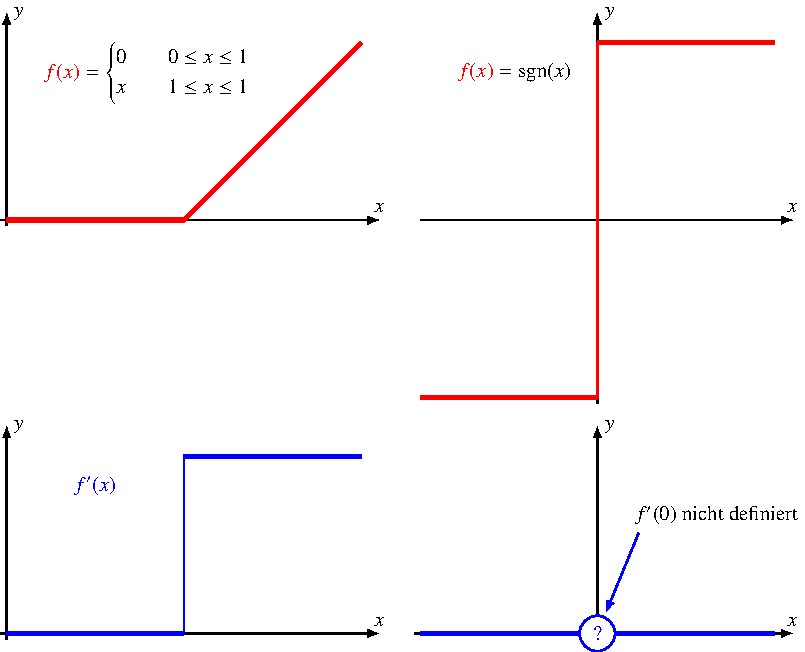
\includegraphics{chapters/010-skalarprodukt/images/schwach.pdf}
\caption{Schwache Ableitung einer nicht differenzierbaren Funktion.
Links die schwache Ableitung der Funktion von
Beispiel~\ref{buch:skalarprodukt:sobolevraum:bsp:schwachexistiert}.
Für die Signum-Funktion von
Beispiel~\ref{buch:skalarprodukt:sobolevraum:bsp:schwachexistiertnicht}
existiert die schwache Ableitung nicht, sie lässt für den Punkt $0$
nicht definieren.
\label{buch:skalarprodukt:sobolevraum:fig:schwach}}
\end{figure}
%
Die in Abbildung~\ref{buch:skalarprodukt:sobolevraum:fig:schwach} links
dargestellte Funktion
\[
f\colon (0,1) \to \mathbb{R}
:
x \mapsto
\begin{cases}
x&\qquad\text{für $0<x<1$}\\
1&\qquad\text{für $1\le x<2$}
\end{cases}
\]
ist stetig und integrierbar, aber sie ist an der Stelle $x=1$ nicht
differenzierbar.
Wir suchen die schwache Ableitung $v$ von $f$.

In einer Umgebung eines Punktes $x>1$ können wir Testfunktionen $\varphi$
so wählen, dass ihr Träger vollständig im Inneren des Intervals $(1,2)$
enthalten ist.
Mit diesen Testfunktionen können wir so rechnen, wie wenn $f$ die konstante
Funktion $1$ ist.
Das bedeutet für das Skalarprodukt
\[
\langle f,\varphi'\rangle
=
\int_1^2 \varphi'(x)\,dx
=
[\varphi(x)]_0^1 = 0.
\]
Das Skalarprodukt mit jeder beliebigen Testfunktion ist $0$, wir
müssen also $v(x)=0$ wählen.

Für $x$ im Teilinterval $(0,1)$ können wir die Testfunktionen so wählen,
dass der Träger vollständig im Inneren  von $(0,1)$ enthalten ist und
somit $f$ als die beliebig oft stetig differenzierbare Funktion $x$
behandelt werden darf.
Für das Skalarprodukt folgt dann
\[
-\langle f,\varphi'\rangle
=
-\int_0^1 f(x)\,\varphi'(x)\,dx
=
-\int_0^1 x\varphi'(x)\,dx
=
-[x\varphi(x)]_0^1 +\int_0^1 \varphi(x)\,dx
=
\langle 1,\varphi(x)\rangle,
\]
in diesem Teil des Intervals muss die schwache Ableitung den Wert $1$ 
haben.

Wir haben somit gefunden, dass die schwache Ableitung von $f$ die
Funktion
\[
v(x) = \begin{cases}
1&\qquad\text{für $0\le x<1$}
\\
0&\qquad\text{für $1< x<2$}
\end{cases}
\]
ist.
Wir kontrollieren dies, indem wir das Skalarprodukt für beliebige 
Testfunktionen $\varphi$ nachrechnen:
\begin{align*}
\langle v,\varphi\rangle
&=
\int_0^2 v(x)\,\varphi(x)\,dx
=
\int_0^1 1\,\varphi(x)\,dx
+
\int_1^2 0\,\varphi(x)\,dx.
\intertext{Jedes dieser Integrale kann man partiell integrieren:}
&=
[x\varphi(x)]_0^1 - \int_0^1 x\varphi'(x)\,dx
+
[1\varphi(x)]_1^2 - \int_1^2 1\varphi'(x)\,dx
\\
&=
\varphi(1) + \varphi(2) - \varphi(1) - \int_0^2 f(x)\,\varphi'(x)\,dx.
\intertext{Da $2$ ein Randpunkt ist, ist $\varphi(2)=0$, so dass sich}
&=-\langle f,\varphi'\rangle.
\end{align*}
ergibt.
Die Funktion $v$ ist also die schwache Ableitung von $f$.
\end{beispiel}

Eine Funktion in $W^{1,2}(\Omega)$ hat eine schwache Ableitung,
wie das Beispiel gezeigt hat, muss die Ableitung keine stetige
Funktion sein.
Ausserdem ist jede andere Funktion, die sich von der schwachen
Ableitung auf einer Menge vom Mass 0 unterscheidet, genauso eine
schwache Ableitung.
Trotzdem kann eine Funktion mit einer schwachen Ableitung nicht
beliebig ``wild'' sein, wie das folgende Beispiel zeigt.

\begin{beispiel}
\label{buch:skalarprodukt:sobolevraum:bsp:schwachexistiertnicht}
Die Signum-Funktion
\[
f\colon (-1,1) = \operatorname{sgn}(x) =
\begin{cases}
         - 1&\qquad\text{für $-1<x<0$}\\
\phantom{-}0&\qquad\text{für $x=0$}\\
\phantom{-}1&\qquad\text{für $0<x<1$}
\end{cases}
\]
ist nicht stetig (Abbildung~\ref{buch:skalarprodukt:sobolevraum:fig:schwach}).
$f$ ist fast überall konstant, in beiden Teilintervallen $(-1,0)$ und
$(0,1)$ ist die einzige mögliche schwache Ableitung von $f$ die
Nullfunktion.
Trotzdem kann $0$ nicht die schwache Ableitung von $f$ sein.
Wir wählen eine Testfunktion $\varphi$, die im Punkt $x=0$ von
Null verschieden ist.
Wäre $v$ eine schwache Ableitung von $f$, dann müsste
\begin{align*}
\langle v,\varphi\rangle
&=
-\langle f,\varphi'\rangle
=
-\int_{-1}^1 f(x) \varphi'(x)\,dx
\\
&=
-\int_{-1}^0 (-1)\cdot \varphi'(x)\,dx
-\int_{0}^1 1\cdot \varphi'(x)\,dx
=
\int_{-1}^0 \varphi'(x)\,dx
-
\int_{0}^1 \varphi'(x)\,dx
\\
&=
[\varphi(x)]_{-1}^0
-
[\varphi(x)]_{0}^1
=
\varphi(0)-\varphi(-1)
-
\varphi(1)+\varphi(0)
\\
&=
2\varphi(0)
\ne 0.
\end{align*}
Andererseits ist die Nullfunktion der einzige Kandidat für die
schwache Ableitun, für die das Skalarprodukt $\langle v,\varphi\rangle=0$
ist.
Dieser Widerspruch zeigt, dass die Funktion $f$ kein schwache
Ableitung hat.
\end{beispiel}

Die schwache Ableitung ermöglicht also mit gewissen Funktionen zu arbeiten,
die keine Ableitung im traditionellen Sinne haben.
Dank der Definition mit Hilfe eines Skalarproduktes in einem 
Hilbert-Raum darf man sich die Funktionen als Grenzwerte von
Cauchy-Folgen vorstellen.

%
% Physikalische Rechtfertigung
%
\subsection{Physikalische Rechtfertigung der schwachen Ableitung}
Die schwache Ableitung ersetzt die mit Hilfe eines Differenzenquotienten
definierte Änderungsrate durch eine Änderungsrate, die durch Vergleich
mit einer in der Umgebung eines Punktes konzentrierten Testfunktion
ermittelt wird.
Auf den ersten Blick mag das als Konzession an die Präzision der Ideen
der Analysis erscheinen, die Newton erfunden hat, um die Physik auf eine
neue Grundlage zu stellen.
Dabei wird aber vergessen, dass der Differenialquotient eine physikalisch
nicht erreichbare Idealisierung darstellt.
Keine Messung kann in einem Punkt im geometrischen Sinn erfolgen.
Die Bestimmung einer Position eines Massepunktes zum Beispiel erfolgt
durch Beobachtung des Lichtes, das vom Massepunkt reflektiert wird.
Doch der Massepunkt ist kein Punkt im geometrischen Sinn, er ist ausgedehnt
über ein endliches Gebiet.
Auch ist die Messung nicht instantan, es wird Licht gemessen, welches
über ein Zeitintervall vom Massepunkt reflektiert wird.
Das Messresultat entsteht also notwendigerweise als Mittelwert der
Beobachtung einer sehr grossen Zahl von Photonen, die von verschiedenen
Stellen reflektiert wurden.
Ein solcher Mittelwert ist genau das, was ein Skalarprodukt
$\langle f,\varphi\rangle$ mit einer Testfunktion ermittelt.

Die Feldgleichungen der Elektrodynamik wurden von Maxwell ausgehend
von Faradays Ideen als partielle Differentialgleichungen formuliert.
Sie verknüpfen die Werte des elektrischen Feldes $\vec{E}$ und des
magnetischen Feldes $\vec{B}$ mit der Ladungsdichte $\varrho$
und der Stromdichte $\vec{\jmath}$, die die Felder erzeugen.
Doch sowohl die Ladungsdichte wie auch die Stromdichte sind Idealisierungen.
Ladungen und Ströme sind nicht stetig über den Raum verteilt, sondern 
in Elektronen oder Atomkernen konzentriert.
Die Ladungsdichte entsteht daraus durch Messung der Ladung in einem kleine
Raumgebiet und Mittelung, was man wieder als Skalarprodukt mit einer
Testfunktion beschreiben kann.

Das elektrische Feld wird gemessen, indem die Kraft auf eine Testladung
im Feld ermittelt wird.
Ausser den prinzipiellen Einschränkungen an die Genauigkeit der
Positionsmessung wissen wir auch aus der Quantenmechanik, dass so etwas
wie die exakte Position eines Teilchens nicht gibt, wir können nur eine
Wahrscheinlichkeitsverteilung dafür bekommen.
Die Kraft äussert sich in einer Geschwindigkeitsänderung, die aber erst
messbar wird, wenn man die Beschleunigung eine gewisse Zeit lang aufrecht
erhält.
Das Messresultat ist also wieder ein Mittelwert über viele Positionen
und Zeitpunkte, oder anders ausgedrückt ein Skalarprodukt mit einer
Testfunktion.

Weitere Beispiele kann man auch in der Fluiddynamik finden.
Die Navier-Stokes-Gleichungen beschreiben die Strömung eines Mediums
unter der Annahme, dass es durch die Dichte $\varrho$ und die
Geschwindigkeit exakt beschreiben lässt.
Das Medium setzt sich aber aus einzelnen Atomen zusammen, die Dichte
ist also bereits ein Mittelwertbildung.
Bei der Geschwindigkeit wird das Problem noch deutlicher.
Auch die Strömungsgeschwindigkeit eines Gases ist der Mittelwert der
Strömungsgeschwindigkeit der Teilchen. 
Die Geschwindigkeit einzelner Teilchen ist dabei meistens sehr viel
grösser, nämlich im Bereich der Schallgeschwindigkeit, und äussert sich
in der Temperatur des Gases, also der mittleren kinetischen Energie.
Es ist nicht sinnvoll, von der Temperatur eines einzelnen Atoms zu
sprechen.

Alle diese Beispiele zeigen, dass die Ableitung als Änderungsrate, die
mit einem Differenzenquotienten bestimmt werden kann, eine Idealisierung
ist.
Wir können dies sogar etwas formeller zeigen.
Sei $x(t)$ die Koordinate eines Massepunktes zur Zeit $t$.
Die Messung kann nicht instantan erfolgen, im besten Fall ist die
gemessene Position ein Integral der Form
\[
\hat{x}(t)
=
\int_{-\infty}^\infty x(\tau) \varphi(\tau - t)\,d\tau.
\]
Darin ist $\varphi$ eine Testfunktion mit Träger in der Nähe von $0$.
Schreiben wir $T_t\varphi(\tau) = \varphi(\tau -t)$, dann können wir
das Messresultat auch als Skalarprodukt
$\hat{x}(t)=\langle x,T_t\varphi\rangle$
schreiben.
Die Messung mit der gleichen Aparatur einen Moment $\Delta t$ später ergibt
\[
\hat{x}(t+\Delta t)
=
\int_{-\infty}^\infty x(\tau) \varphi(\tau-t-\Delta t)\,dt
=
\langle x, T_{t+\Delta t}\varphi\rangle.
\]
Die Geschwindigkeit als Differenzenquotient ist
\begin{equation}
\frac{
\hat{x}(t+\Delta t)-\hat{x}(t)
}{\Delta t}
=
\frac{
\langle f,T_{t+\Delta t}\varphi\rangle
-
\langle f,T_{t}\varphi\rangle
}{
\Delta t
}
=
\left\langle
f,\frac{T_{t+\Delta t}\varphi - \varphi}{\Delta t}
\right\rangle
\label{buch:skalarprodukt:sobolevlraum:eqn:geschwindigkeit}
\end{equation}
Die Funktion $(T_{t+\Delta t}\varphi-T_t\varphi)/\Delta t$ ist eine 
beliebig oft stetig differenzierbare Funktion, die im Grenzwert
$\Delta t\to 0$ gegen
\[
\frac{
\varphi(\tau - t - \Delta t)
-
\varphi(\tau - t)
}{
\Delta t
}
=
-
\frac{
\varphi(\tau - t + \delta) - \varphi(\tau - t)
}{
\delta
}
\to 
-
\varphi'(\tau - t)
\quad
\text{für $\delta = - \Delta \to 0$}
\]
konvergiert.
Der Differenzenquotient
\eqref{buch:skalarprodukt:sobolevlraum:eqn:geschwindigkeit}
konvergiert daher gegen
\[
\lim_{\Delta t\to 0}
\frac{
\hat{x}(t+\Delta t)-\hat{x}(t)
}{\Delta t}
=
\left\langle
x,
\lim_{\Delta t\to 0}
\frac{T_{t+\Delta t}\varphi-T_t\varphi}{\Delta t}
\right\rangle
=
\langle f,-\varphi'\rangle
=
-
\langle f, \varphi'\rangle.
\]
Dieses einfache Modell einer ``unscharfen'' Messung führt also automatisch
auf das Konzept der schwachen Ableitung.








%\uebungsabschnitt
%\aufgabetoplevel{chapters/010-potenzen/uebungsaufgaben}
%\begin{uebungsaufgaben}
%\uebungsaufgabe{101}
%\uebungsaufgabe{102}
%\uebungsaufgabe{103}
%\uebungsaufgabe{104}
%\end{uebungsaufgaben}
%\endgroup


%
% chapter.tex -- Skalarprodukt
%
% (c) 2021 Prof Dr Andreas Müller, Hochschule Rapperswil
%
% !TeX spellcheck = de_CH
\chapter{Skalarprodukte
\label{buch:chapter:skalarprodukte}}
\kopflinks{Skalarprodukte}

%
% 1-definition.tex
%
% (c) 2023 Prof Dr Andreas Müller, OST Ostschweizer Fachhochschule
%
\section{Definition
\label{buch:opertoren:section:definition}}
\kopfrechts{Definition}


%
% 2-cauchyschwarz.tex
%
% (c) 2022 Prof Dr Andreas Müller, OST Ostschweizer Fachhochschule
%
\section{Ungleichungen
\label{buch:skalarprodukte:section:cauchyschwarz}}
\kopfrechts{Cauchy-Schwarz-Ungleichung}
In der Vektorgeometrie wird gelehrt, dass die Länge eines Vektors $u$
durch die Norm $\|u\|$ wiedergegeben wird und dass die geometrische
Intuition dazu passt.
Dazu gehört vor allem, dass die Dreiecksungleichung erfüllt ist,
dass also für drei Punkt $A$, $B$ und $C$
\begin{equation}
\overline{AB} \le \overline{AC} + \overline{BC}
\label{skalarprodukt:ungleichungen:eqn:dreieck}
\end{equation}
gilt.
In Vektorform bedeutet dies, dass
\[
\| b-a\|
\le
\| c-a\| + \|b-c\|.
\]
Schreibt man $u=c-a$ und $v=b-c$, dann ist $u+v=b-a$ und somit
\begin{equation}
\| u+v\| \le \|u\| + \|v\|.
\label{skalarprodukt:cauchyschwarz:eqn:dreieck0}
\end{equation}
Dies ist die Dreiecksungleichung in
Vektorform~\eqref{skalarprodukt:cauchyschwarz:eqn:dreieck0}.
Ziel dieses Abschnitts ist zu zeigen, dass jedes reelle oder
komplexe Skalarprodukt diese und weitere Eigenschaften automatisch
mitbringt.

%
% Cauchy-Schwarz-Ungleichung
%
\subsection{Cauchy-Schwarz-Ungleichung}
Sei also $\langle\;\,,\;\rangle$ ein reelles oder komplexes Skalarprodukt
auf dem Vektorraum $V$,
insbesondere ist $\langle v,v\rangle\ge 0$ für beliebige Vektoren $v\in V$.
Für zwei Vektoren $x,y\in V$ und $t\in \mathbb{R}$  gilt daher
\begin{align}
0
&\le
\| x+ty\|^2
=
\langle x+ty,x+ty\rangle
=
\langle x,x\rangle
+
t\langle x,y\rangle
+
t\langle y,x\rangle
+
t^2
\langle y,y\rangle.
\label{skalarprodukt:cauchyschwarz:eqn:quadrat}
\end{align}
Für ein reelles Skalarprodukt ist $\langle x,y\rangle=\langle y,x\rangle$
und damit
\begin{align}
0
&\le
\|x\|^2 + 2t\langle x,y\rangle + t^2 \|y\|^2.
\label{buch:skalarprodukt:cauchyschwarz:eqn:cspoly}
\end{align}
Dies ist ein quadratisches Polynom in der Variablen $t$, dessen Minimum
nicht negativ sein darf.

%
% Minimum eines quadratischen Polynoms
%
\subsubsection{Minimum eines quadratischen Polyoms}
Ein beliebiges quadratisches Polynom
\[
p(t)=at^2+bt+c
\]
kann durch
quadratisches Ergänzen in die Form
\[
p(t)
=
a\biggl(t+\frac{b}{2a}\biggr)^2 -\frac{b^2}{4a}+c
\]
gebracht werden.
Daraus kann man ablesen, dass das Minimum an der Stelle
\[
t_0
=
-\frac{b}{2a}
\]
angenommen wird und den Wert 
\begin{equation}
p(t_0)
=
c-\frac{b^2}{4a}
\end{equation}
hat.
Die gleiche Lösung kann natürlich auch durch Bestimmung des Minimums
von $p(t)$ mit Hilfe der Bedingung $p'(t_0)=0$ gefunden werden.

%
% Cauchy-Schwarz-Ungleichung für einen reellen Vektorraum
%
\subsubsection{Cauchy-Schwarz-Ungleichung für einen reellen Vektorraum}
Für~\eqref{buch:skalarprodukt:cauchyschwarz:eqn:cspoly}
ist
\[
a=\|y\|^2,\quad
b=2\langle x,y\rangle
\quad\text{und}\quad
c=\|x\|^2.
\]
Daher folgt aus~\eqref{buch:skalarprodukt:cauchyschwarz:eqn:cspoly}
\[
0
\le
\|x\|^2 - \frac{\langle x,y\rangle^2}{\|y\|^2}
\qquad\Rightarrow\qquad
\langle x,y\rangle^2 \le \|x\|^2\, \|y\|^2
\qquad\Rightarrow\qquad
|\langle x,y\rangle| \le \|x\|\, \|y\|.
\]
Dies ist die Cauchy-Schwarz-Ungleichung für das Skalarprodukt
$\langle \;\,,\;\rangle$.

\begin{satz}[Cauchy-Schwarz]
\label{buch:skalarprodukt:cauchy-schwarz:satz:reell}
Ein reelles Skalarprodukt $\langle\;\,,\;\rangle$ auf dem reellen Vektorraum
$V$ erfüllt die Cauchy-Schwarz-Ungleichung
\[
|\langle x, y\rangle| \le \|x\|\,\|y\|
\]
für $x,y\in V$.
\end{satz}

%
% Cauchy-Schwarz-Ungleichung für einen komplexen Vektorraum
%
\subsubsection{Cauchy-Schwarz-Ungleichung für einen komplexen Vektorraum}
Für ein komplexes Skalarprodukt ist das Produkt $\langle x,y\rangle$
nicht mehr unbedingt reell und kann damit nicht mehr direkt mit den
Normen $\|x\|^2u$ und $\|y\|^2$ vergleichen.
Wir ersetzen daher $t$ durch
$t\langle y,x\rangle=t\overline{\langle x,y\rangle}$
und erhalten 
\begin{align*}
0
\le
\|x+t\langle y,x\rangle y\|^2
&=
\langle x,x\rangle
+t\langle y,x\rangle \langle x,y\rangle
+t\overline{\langle y,x\rangle}\langle y,x\rangle
+t^2\langle y,y\rangle
\\
&=
\|x\|^2
+
t
2|\langle x,y\rangle|^2
+
t^2 |\langle x,y\rangle|^2
\|y\|^2.
\end{align*}
Dies ist wieder ein quadratisches Polynom, diesmal mit den Koeffizienten
\[
a= |\langle x,y\rangle|^2 \|y\|^2,
\quad
b= 2|\langle x,y\rangle|^2
\quad\text{und}\quad
c= \|x\|^2.
\]
Das Minimum dieses Polynoms ist nach
\[
0
\le
c-\frac{b^2}{4a}
=
\|x\|^2 - \frac{|\langle x,y\rangle|^4}{|\langle x,y\rangle|^2\,\|y\|^2}
=
\|x\|^2 - \frac{|\langle x,y\rangle|^2}{\|y\|^2}
\quad\Rightarrow\quad
|\langle x,y\rangle|^2 \le \|x\|^2\,\|y\|^2
\quad\Rightarrow\quad
|\langle x,y\rangle \le \|x\|\,\|y\|.
\]
Dies ist die Cauchy-Schwarz-Ungleichung für einen komplexen Vektorraum.

\begin{satz}[Cauchy-Satz]
\label{buch:skalarprodukt:cauchy-schwarz:satz:komplex}
Ein komplexes Skalarprodukt $\langle\;\,,\;\rangle$ auf dem komplexen Vektorraum
$V$ erfüllt die Cauchy-Schwarz-Ungleichung
\[
|\langle x, y\rangle| \le \|x\|\,\|y\|
\]
für $x,y\in V$.
\end{satz}

Man beachte, dass die
Sätze~\ref{buch:skalarprodukt:cauchy-schwarz:satz:reell}
und
\ref{buch:skalarprodukt:cauchy-schwarz:satz:komplex}
nur die Axiome eines Skalarproduktes verwenden.
Sie gelten also
ganz unabhängig von der konkreten Definition des Skalarproduktes,
solange die Eigenschaften eines Skalarproduktes gegeben sind.

\begin{beispiel}
Die sesquilineare Funktion
\[
\langle x,y\rangle
=
\sum_{i=1}^n\overline{x}_i y_i
\]
für Vektoren $x,y\in\mathbb{C}^n$ ist positiv definit, denn
\[
\langle x,x\rangle
=
\sum_{i=1}^n \overline{x}_i x_i = \sum_{i=1}^n |x_i|^2 > 0
\]
für $x\ne 0$.
Nach Satz~\ref{buch:skalarprodukt:cauchy-schwarz:satz:komplex}
gilt daher
\[
\biggl|
\sum_{i=1}^n \overline{x}_i y_i
\biggr|
\le
\sqrt{\sum_{i=1}^n |x_i|^2} \sqrt{\sum_{i=1}^n |y_i|^2}
\quad\text{oder auch}\quad
\biggl|
\sum_{i=1}^n x_i y_i
\biggr|
\le
\sqrt{\sum_{i=1}^n |x_i|^2} \sqrt{\sum_{i=1}^n |y_i|^2}
\]
für beliebige Vektoren $x,y\in\mathbb{C}^n$.
\end{beispiel}

\begin{beispiel}
Die sesquilineare Funktion
\[
\langle f,g\rangle
=
\int_a^b \overline{f(x)} g(x)\,dx
\]
für komplexwertige, stetige Funktion auf dem Intervall $[a,b]$
ist positiv definit, denn
\[
\langle f,f\rangle
=
\int_a^b \overline{f(x)} f(x)\,dx
=
\int_a^b |f(x)|^2\,dx
\ge 0
\]
für $f\ne 0$.
Nach Satz~\ref{buch:skalarprodukt:cauchy-schwarz:satz:komplex}
gilt daher
\begin{align*}
\biggl|\int_a^b \overline{f(x)}g(x)\,dx\biggr|
&\le
\sqrt{\int_a^b |f(x)|^2\,dx}
\sqrt{\int_a^b |g(x)|^2\,dx}
\intertext{oder auch}
\biggl|\int_a^b f(x) g(x)\,dx\biggr|
&\le
\sqrt{\int_a^b |f(x)|^2\,dx}
\sqrt{\int_a^b |g(x)|^2\,dx}
\end{align*}
für beliebige komplexwertige stetige Funktionen $f,g$ auf dem
Intervall $[a,b]$.
\end{beispiel}

%
% Dreiecksungleichung
%
\subsection{Dreiecksungleichung}
Die Intuition einer Längenmessung basiert auf der
Dreiecksungleichung~\eqref{skalarprodukt:ungleichungen:eqn:dreieck}.
Sie ist gleichbedeutend mit der
Vektorform~\eqref{skalarprodukt:cauchyschwarz:eqn:dreieck0}
der Ungleichung.

Die Cauchy-Schwarz-Ungleichung ermöglicht nun, diese Ungleichung
nachzurechnen.
Die Norm von $\|x+y\|^2$ ist
\[
\|x+y\|^2
=
\langle x+y,x+y\rangle
=
\langle x,x\rangle
+
\langle x,y\rangle
+
\langle y,x\rangle
+
\langle y,y\rangle
=
\|x\|^2 + 2\operatorname{Re}\langle x,y\rangle + \|y\|^2.
\]
Den mittleren Term kann man mit der Cauchy-Schwarz-Ungleichung
umformen:
\begin{align*}
\|x\|^2 + 2\operatorname{Re}\langle x,y\rangle + \|y\|^2.
&\le
\|x\|^2 + 2|\operatorname{Re}\langle x,y\rangle| + \|y\|^2.
\\
&\le
\|x\|^2 + 2|\langle x,y\rangle| + \|y\|^2.
\\
&\le
\|x\|^2 + 2\|x\|\,\|y\| + \|y\|^2
=
(\|x\| + \|y\|)^2.
\end{align*}
Durch Ziehen der Wurzel folgt
\[
\|x+y\| \le \|x\| + \|y\|.
\]
Damit ist der folgende Satz bewiesen.

\begin{satz}[Dreiecksungleichung]
Für die Norm zu einem beliebigen Skalarprodukt auf dem reellen
oder komplexen Vektorraum $V$ gilt die Dreiecksungleichung
\[
\|x+y\| \le \|x\| + \|y\|
\]
für $x,y\in V$.
\end{satz}

%
% Normen
%
\subsection{Normen
\label{skalarprodukt:cauchyschwarz:subsection:norm}}
Das Skalarprodukt ist nicht die einzige Möglichkeit, eine Norm auf
einem Vektorraum zu definieren.
Zum Beispiel kann man auf $\mathbb{C}^n$ die sogenannte $l^1$-Norm
definieren.

\begin{definition}
Die Funktion
\[
\|x\|_1
=
\sum_{i=1}^n |x_i|
\]
für $x\in\mathbb{C}^n$ heisst die {\em $l^1$-Norm} auf $\mathbb{C}^n$.
\end{definition}

Die Funktion $\|\cdot\|_1$ ist eine Norm im Sinne der folgenden Definition.

\begin{definition}
Eine Funktion $\|\cdot\| \colon V\to\mathbb{R}$ auf einem reellen
oder komplexen Vektorraum $V$ heisst eine {\em Norm}, wenn Sie die
folgenden Bedingungen erfüllt
\begin{enumerate}
\item
$\|\lambda x\| = |\lambda|\, \|x\|$ für $x\in V$ und $\lambda\in \Bbbk$
\item
Für alle Vektoren $x\in V$ mit $x\ne 0$ gilt $\|x\|>0$.
\item
Dreiecksungleichung: $\|x+y\| \le \|x\| + \|y\|$ für alle $x,y\in V$
\end{enumerate}
\end{definition}

Es ist klar, dass die $l^1$-Norm die Bedingungen~1 und 2 erfüllt.
Aber auch die Bedingung~3 kann man leicht  nachprüfen:
\[
\|x+y\|_1
=
\sum_{i=1}^n |(x+y)_i|
=
\sum_{i=1}^n |x_i+y_i|
\le
\sum_{i=1}^n(|x_i|+|y_i|)
=
\sum_{i=1}^n|x_i|
+
\sum_{i=1}^n|y_i|
=
\|x\|_1 + \|y\|_1,
\]
wozu wir nur die Dreiecksungleichung $|a+b|\le |a| + |b|$ für reelle 
oder komplexe Zahlen $a,b$ benötigen.

\begin{beispiel}
Die Funktion
\[
\|x\|_\infty = \sup_{1\le i\le n} |x_i|
\]
ist eine Norm auf $\mathbb{C}^n$.
\end{beispiel}

Auch in diesem Fall sind die Bedingungen~1 und 2 ganz offensichtlich erfüllt.
Für die Dreiecksungleichung rechnen
\begin{align*}
\|x+y\|_\infty
&=
\sup_{1\le i\le n} |x_i+y_i|
\le
\sup_{1\le i\le n} (|x_i|+|y_i|)
\le
\sup_{1\le i\le n} |x_i|+\sup_{1\le i\le n}|y_i|
=
\|x\|_\infty + \|y\|_\infty.
\end{align*}
Somit ist $\|\cdot\|_\infty$ eine Norm auf $\mathbb{C}^n$.

%
% Polaridentität
%
\subsection{Polaridentität}
Die durch das Skalarprodukt definierte Norm
\( \|x\|^2=\langle x,x\rangle \)
ist nach Abschnitt~\ref{skalarprodukt:cauchyschwarz:subsection:norm}
ein Spezialfall einer Norm.
Ist es möglich, für eine Norm, die von einem Skalarprodukt herkommt,
das Skalarprodukt wieder zu rekonstruieren?

%
% Reelles Skalarprodukt aus der Norm
%
\subsubsection{Reelles Skalarprodukt aus der Norm}
Die Antwort gibt der folgende Satz.

\begin{satz}[Polaridentität]
\label{skalarprodukt:cauchyschwarz:satz:polarformel}
Ist $\|\cdot\|$ die Norm zu einem Skalarprodukt auf dem reellen Vektorraum
$V$, dann kann das Skalarprodukt zweier Vektoren $x,y\in V$ mittels
der sogenannten {\em Polaridentität}
\index{Polaridentität}%
\begin{equation}
\langle x, y\rangle
=
\frac12\bigl(
\|x+y\|^2 - \|x\|^2 - \|y\|^2 
\bigr)
\label{skalarprodukt:cauchyschwarz:eqn:polar}
\end{equation}
berechnet werden.
\end{satz}

\begin{proof}[Beweis]
Die Gleichung
\begin{align*}
\|x+y\|^2
&=
\langle x+y,x+y\rangle
=
\|x\|^2 + 2\langle x,y\rangle + \|y\|^2 
\end{align*}
kann nach $\langle x,y\rangle$ aufgelöst werden und ergibt
die behauptete Formel~\eqref{skalarprodukt:cauchyschwarz:eqn:polar}.
\end{proof}

% 
% Parallelogrammgleichung
%
\subsubsection{Parallelogrammgleichung}
\begin{figure}
\centering
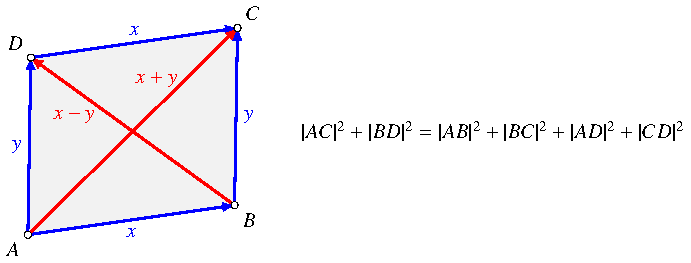
\includegraphics{chapters/010-skalarprodukt/images/parallelogramm.pdf}
\caption{Parallelogrammregel für eine Norm, die aus einem Skalarprodukt
entsteht.
\label{skalarprodukt:cauchyschwarz:fig:parallelogramm}}
\end{figure}
Die Polaridentitäten können auch noch in einer anderen Form geschrieben
werden.
Dazu berechnet man zusätzlich die Norm von $x-y$:
\begin{align*}
\|x+y\|^2
&=
\|x\|^2 + \|y\|^2 + 2\langle x, y\rangle
\\
\|x-y\|^2
&=
\|x\|^2 + \|y\|^2 - 2\langle x, y\rangle
\\
\|x+y\|^2 +\|x-y\|^2
&=
2\|x\|^2 + 2\|y\|^2
\end{align*}

\begin{satz}
\label{skalarprodukt:cauchyschwarz:satz:parallelgramm}
Für eine Norm, die von einem reellen Skalarprodukt herkommt, gilt die
Parallelogrammformel
\begin{equation}
\|x+y\|^2 +\|x-y\|^2
=
2\|x\|^2 + 2\|y\|^2.
\label{skalarprodukt:cauchyschwarz:eqn:parallelgramm}
\end{equation}
(Abbildung~\ref{skalarprodukt:cauchyschwarz:fig:parallelogramm})
\end{satz}

Das Skalarprodukt kann man damit auf verschiedene Weise aus der
Norm gewinnen:
\begin{equation}
\begin{aligned}
\langle x, y\rangle
&=
{\textstyle\frac12}\bigl( \|x\|^2 + \|y\|^2 - \|x+y\|^2 \bigr)
\\
&=
{\textstyle\frac12}\bigl(
\|x+y\|^2
-
\|x\|^2 
-
\|y\|^2
\bigr)
\\
&=
{\textstyle\frac14}\bigl(
\|x+y\|^2 - \|x-y\|^2
\bigr).
\end{aligned}
\label{skalarprodukt:cauchyschwarz:eqn:realteil}
\end{equation}
Nur die letzte Formel ist noch nicht gut begründet.
Man kann aber sofort nachrechnen, dass 
\begin{align*}
\|x+y\|^2&=\|x\|^2+2\langle x,y\rangle+\|y\|^2\\
\|x-y\|^2&=\|x\|^2-2\langle x,y\rangle+\|y\|^2
\intertext{die Differenz}
\|x+y\|^2 - \|x-y\|^2 &= 4\langle x,y\rangle
\qquad
\Rightarrow
\qquad
\langle x,y\rangle
=
\frac14\bigl(\|x+y\|^2 - \|x-y\|^2\bigr)
\end{align*}
haben.

%
% Komplexes Parallelogramm aus der Norm
%
\subsubsection{Komplexe Skalarprodukt}
Das Resultat von Satz~\ref{skalarprodukt:cauchyschwarz:satz:polarformel}
gilt in abgeänderter Form auch für komplexe Skalarprodukte.
Da das Skalarprodukt auch einen nichtverschwindenen Imaginärteil haben
kann, wird eine zusätzliche Gleichung zur Berechnung des Imaginärteils
nötig.
Eine solche kann gewonnen werden, indem zusätzlich die Normen
$\|x+iy\|^2$ und $\|x-iy\|^2$ berechnet werden.
Dazu ist zu beachten, dass
\[
\langle x,y\rangle
-
\langle y,x\rangle
=
\langle x,y\rangle
-
\overline{
\langle x,y\rangle
}
=
2i\operatorname{Im}\langle x,y\rangle
\]
Damit erhält man
\begin{align*}
\|x+iy\|^2 &= \|x\|^2 + i\langle x,y\rangle - i\langle y,x\rangle + \|y\|^2 
           = \|x\|^2 + 2\operatorname{Im}\langle x,y\rangle + \|y\|^2 \\
\|x-iy\|^2 &= \|x\|^2 - i\langle x,y\rangle + i\langle y,x\rangle + \|y\|^2 
           = \|x\|^2 - 2\operatorname{Im}\langle x,y\rangle + \|y\|^2.
\end{align*}
Damit kann man nach dem Imaginärteil des Skalarproduktes auflösen und
die Formeln
finden, die den Formeln
\eqref{skalarprodukt:cauchyschwarz:eqn:realteil}
für das reelle Skalarprodukt entsprechen.
\eqref{skalarprodukt:cauchyschwarz:eqn:realteil}
Formeln bleiben gültig als Formeln für den Realteil des Skalarproduktes.
Damit haben wir den folgenden Satz gefunden.

\begin{satz}[Polaridentitäten für ein komplexes Skalarprodukt]
Ist $\|\cdot\|$ die Norm, die aus dem komplexen Skalarprodukt
$\langle\;\,,\;\rangle$ auf einem Vektorraum $V$ gewonnen wurde,
dann können Real- und Imaginärteil mit den Formeln
\begin{align*}
\operatorname{Re}\langle x,y\rangle
&=
{\textstyle\frac12}\bigl(
\|x+y\|^2 - \|x\|^2 -\|y\|^2
\bigr)
\\
&=
{\textstyle\frac12}\bigl(
\|x\|^2 +\|y\|^2 - \|x+y\|^2
\bigr)
\\
&=
{\textstyle\frac14}\bigl(
\|x+y\|^2 - \|x-y\|^2
\bigr),
\\
\operatorname{Im}\langle x,y\rangle
&=
{\textstyle\frac12}\bigl(
\|x+iy\|^2-\|x\|^2-\|y\|^2
\bigr)
\\
&=
{\textstyle\frac12}\bigl(
\|x\|^2+\|y\|^2-\|x-iy\|^2
\bigr)
\\
&=
{\textstyle\frac14}\bigl(
\|x+iy\|^2
-
\|x-iy\|^2
\bigr)
\end{align*}
für beliebige Vektoren $x,y\in V$
allein aus Werten der Norm berechnet werden.
\end{satz}


%
% 3-funktionenraeume.tex
%
% (c) 2022 Prof Dr Andreas Müller, OST Ostschweizer Fachhochschule
%
\section{Funktionenräume
\label{buch:skalarprodukt:section:funktionenraeume}}
\kopfrechts{Funktionenräume}
Ziel der harmonischen Analysis ist die effiziente Approximation einer
grossen Klasse von Funktionen.
Als approximierende Funktionen kommen stetige Funktionen, Polynome,
trigonometrische Polynome oder eine ähnlich, einfach konstruierbare
Funktionenfamilie in Frage.
Es gilt zunächst herauszufinden, was ``Approximation'' genau heissen
soll und von welchen Funktionen man überhaupt erwarten kann, dass sie
approximiert werden können.

%
% Stetige Funktionen
%
\subsection{Stetige Funktionen
\label{buch:skalarprodukt:subsection:stetige-funktionen}}
Der frühe intuitive Funktionsbegriff ging oft von der Vorstellung einer
in einem Strich gezeichneten Kurve aus, wie man sie von den Graphen
der Polynome oder der trigonometrischen Funktionen her kennt.
In moderner Sprechweise sind dies die stetigen Funktionen.

\begin{definition}
Eine Funktion $f\colon I\to\mathbb{R}$ mit $I\subset \mathbb{R}$
heisst stetig in einem Punkt $x_0\in I$, wenn für jedes $\varepsilon>0$
ein $\delta>0$ existiert derart, dass $f(x)-f(x_0)|<\delta$ sobald
$|x-x_0|<\varepsilon$.
\end{definition}

Nur die Eigenschaft, eine Abstandsmessung zu besitzen, wird vom
Definitionsbereich $I\subset \mathbb{R}$ verlangt.
Der Stetigkeitsbegriff kann daher verallgemeinert werden auf den
Begriff des metrischen Raumes.

\begin{definition}
Eine {\em Metrik} auf einer Menge $X$ ist eine Funktion
\index{Metrik}%
$d\colon X\times X\to \mathbb{R}$
mit den folgenden Eigenschaften
\begin{enumerate}
\item
Positiv definit: $d(x,y)\ge 0$ und $d(x,y)$ genau dann, wenn $x=y$.
\item
Symmetrie: \(d(x,y)=d(y,x)\)
\item
Dreiecksungleichung: \( d(x,y) \le d(x,z) + d(z,y) \).
\end{enumerate}
Ein {\em metrischer Raum} ist ein Menge $X$ mit einer Metrik.
\index{matrischer Raum}%
\end{definition}

In einem metrischen Raum ist der Begriff des Grenzwertes übertragbar.
Mit dem Begriff des Grenzwertes lässt sich auch der Begriff der
Stetigkeit verallgemeinern.

\begin{definition}
Ist $x_n\in X$ eine Folge von Punkten in einem metrischen Raum $X$,
dann heisst $x$ der Grenzwert der Folge $x_n$, wenn es für jedes
$\varepsilon>0$ ein $N>0$ gibt derhart, dass
$d(x_n,x)\le \varepsilon$ für alle $n>N$.
Eine Funktion $f\colon X\to Y$ zwischen metrischen Räumen heisst
stetig im Punkt $x\in X$, wenn für jede Folge $x_n\in X$ mit
Grenzwert $x$ auch die Folge $y_n=f(x_n)\in Y$ konvergiert und
den Grenzwert $y=f(x)$ hat.
\end{definition}

Teilmengen von $\mathbb{R}$ oder $\mathbb{R}^n$ tragen natürlich
die Struktur eines metrischen Raumes mit der Abstandsmessung in 
$\mathbb{R}^n$ als Metrik
\[
d(x,y) = \sqrt{(x_1-y_1)^2 + \ldots + (x_n-y_n)^2} = \|x-y\|.
\]
Die Eigenschaften einer Metrik wurden bereits in Abschnitt
\ref{buch:skalarprodukte:section:cauchyschwarz} nachgewiesen.

Der Begriff des Grenzwertes klärt, was mit der Approximation von $x$
durch eine Folge $x_n$ gemeint ist.
Wenn man darauf aufbauend die Konvergenz einer Folge von Funktionen
gegen eine Grenzfunktion definieren will, braucht man einen Abstansbegriff
zwischen Funktionen.
Ein erster Versuch könnte sein, als Abstand zwischen zwei Funktionen
$f$ und $g$ die Funktion
\[
d(f,g) = |f(x_0) - g(x_0)|.
\]
Die Menge der Funktionen wird dadurch jedoch nicht zu einem metrischen
Raum.
Zwar gilt sicher die Symmetrie und Dreiecksungleichung, und auch 
$d(f,g)\ge 0$ für beliebige Funktionen.
Aber wenn $d(f,g)=0$ ist, heisst das nur, dass $f$ und $g$ im Punkt
$x_0$ den gleichen Wert haben.
Ausser in trivialen Fällen wird es Funktionen geben, die zwar im Punkt
$x_0$ übereinstimmen, sich aber in mindestens einem anderen Punkt
unterscheiden.

%
% Normierte Räume
%
\subsubsection{Normierte Räume}
Die stetigen Funktionen bilden aber keine strukturlose Menge, sie
bilden einen Vektorraum: die Summe von stetigen Funktionen ist ebenfalls
stetig, multiplizieren einer stetigen Funktion mit einem Skalar führt
nicht aus der Menge der stetigen Funktionen heraus.
Die für den Grenzwertbegriff von Funktionen verwendete Abstandsmessung 
sollte der Vektorraumstruktur ebenfalls Rechnung tragen.

\begin{definition}
\label{buch:skalaprodukt:funktionenraume:def:norm}
Sei $V$ ein Vektorraum über $\mathbb{R}$, dann heisst eine Funktion
\( \|\;\cdot\;\| \colon V \to \mathbb{R}\) eine {\em Norm}, wenn gilt
\index{Norm}
\begin{enumerate}
\item
Definit: $ \|x\| = 0 \Rightarrow x=0$
\item
Homogeneität: $ \| \lambda x \| = |\lambda| \cdot \|x\|$
\item
Dreiecksungleichung: $\|x+y\| \le \|x\| + \|y\|$
\end{enumerate}
Ein {\em normierter Raum} ist ein Vektorraum $V$ mit einer Norm.
\end{definition}

%
% Vollständigkeit
%
\subsubsection{Vollständigkeit}
In den rationalen Zahlen hat nicht jede Folge einen Grenzwert.
Die Zahl $\sqrt{2}$ lässt sich beliebig genau durch rationale Zahlen
approximieren, sie ist aber nicht in $\mathbb{Q}$.
Ähnlich lässt sich die Funktion $x\mapsto \sqrt{x}$ beliebig genau 
durch Polyome approximieren, sie ist aber selbst kein Poylnome

\begin{definition}
Ein Folge $x_n\in X$ in einem metrischen Raum heisst {\em Cauchy-Folge},
wenn es für jedes $\varepsilon>0$ ein $N>0$ gibt derart, dass 
$|x_n-x_m|<\varepsilon$ wenn $n,m>N$ ist.
\end{definition}

Cauchy-Folgen sind also Folgen, die sich für genügend grossen Index
kaum mehr ändern und für die man daher Konvergenz erwarten würde.

\begin{definition}
Ein normierter Raum heisst {\em vollständig} oder ein Banach-Raum,
wenn jede Cauchy-Folge einen Grenzwert hat.
\end{definition}

Die rationalen Zahlen $\mathbb{Q}$ bilden keinen vollständigen
metrischen Raum, aber die reellen Zahlen $\mathbb{R}$ enthalten
alle Grenzwerte von Cauchy-Folgen, $\mathbb{R}$ ist eine vollständiger
metrischer Raum.
Die Menge der Polynome, betrachtet als Teilmenge der Menge der
stetigen Funktionen $[0,1]\to\mathbb{R}$ ist nicht vollständig,
da es eine Folge $f_n(x)$ von Approximationsfunktionen der Funktion
$x\mapsto \sqrt{x}$ gibt.
Als Cauchy-Folge konvergiert sie zwar gegen eine stetige Funktion,
aber die Grenzfunktion ist nicht mehr im Raum der Polynome.

Das Ziel der folgenden Kapitel ist also, zu geeignet interessanten
Funktionenfamilien ``gute'' Normen zu finden derart, dass Cauchy-Folgen
konvergieren gegen Funktionen, die immer noch ausreichend viele
nützliche Eigenschaften haben.
Im besten Fall konvergieren stetige Funktionen gegen stetige Funktionen,
es wird sich aber zeigen, dass diese Anforderung zu streng ist.

%
% Norm fpr stetige Funktionen
%
\subsection{Norm für stetige Funktionen
\label{buch:skalarprodukt:subsection:normfuerstetigefunktionen}}
Damit man von Konvergenz von Folgen stetiger Funktionen sprechen kann,
brauchen wir jetzt also eine Norm für stetige Funktionen.

\begin{definition}
Sei $X$ ein metrischer Raum und
\[
C(X)
=
C_{\mathbb{R}}(X)
=
\{
f\colon X \to\mathbb{R}\mid
\text{$f$ ist stetig}
\}
\]
der Vektorraum der stetigen Funktion auf $X$.
Die Norm von $C(X)$ ist definiert als
\[
\|f\| = \sup_{x\in X} |f(x)|.
\]
Sie heisst die {\em Supremum-Norm}.
\end{definition}

Wir prüfen nach, dass die Supremum-Norm tatsächlich eine Norm ist.
Dazu sind die definierenden Eigenschaften nachzurechnen:
\begin{enumerate}
\item Definit: 
\[
0
=
\|f\|
=
\sup_{x\in X} |f(x)|
\quad\Rightarrow\quad
f(x)=0 \;\forall x\in X
\quad\Rightarrow\quad
f\in C(X).
\]
\item Homogeneität:
\[
\|\lambda f\|
=
\sup_{x\in X} |\lambda f(x)|
=
|\lambda| \sup_{x\in X} |f(x)|
=
|\lambda| \cdot \|f\|.
\]
\item
Dreiecksungleichung:
\[
\|f+g\|
=
\sup_{x\in X}|f(x)+g(x)|
\le
\sup_{x\in X}(|f(x)|+|g(x)|)
\le
\sup_{x\in X}|f(x)|+\sup_{x\in X}|g(x)|
=
\|f\| + \|g\|.
\]
\end{enumerate}

Eine Cauchy-Folge $f_n$ von Funktionen $X\to \mathbb{R}$ hat die
Eigenschaft, dass für jedes $\varepsilon >0$ ein $N>0$ existiert,
derart dass $\|f_n-f_m\|<\varepsilon$ ist.
Da die Norm der maximale Unterschied von Funktionswerten ist,
folgt dass für eine Cauchy-Folge in $C(X)$ die Folge $f_n(x)$ eine
Cauchy-Folge in $\mathbb{R}$ ist und damit einen Grenzwert in $\mathbb{R}$
hat.
Die Funktion $f(x) = \lim_{n\to\infty}f_n(x)$ ist die Grenzfunktion.
Die Konvergenz bezüglich der Norm besagt, dass für jedes $\varepsilon>0$
es ein $N>0$ gibt derart, dass
\[
\varepsilon 
>
\|f_n-f\|
\ge 
|f_n(x)-f(x)|
\]
ist für alle $n>N$ und unabhängig von $x\in X$.
Die Konvergenz bezüglich der $\|\;\cdot\;\|$-Norm ist also die wohlbekannte
gleichmässige Konvergenz.
Es kann gezeigt werden, dass die Grenzfunktion wieder stetig ist.

\begin{satz}
Der Raum der stetigen Funktion $C(X)$ mit der Supremumg-Norm ist
ein Banach-Raum.
\end{satz}

%
% Skalarprodukt
%
\subsection{Skalarprodukt
\label{buch:skalarprodukt:subsection:skalarprodukt}}
\begin{figure}
\centering
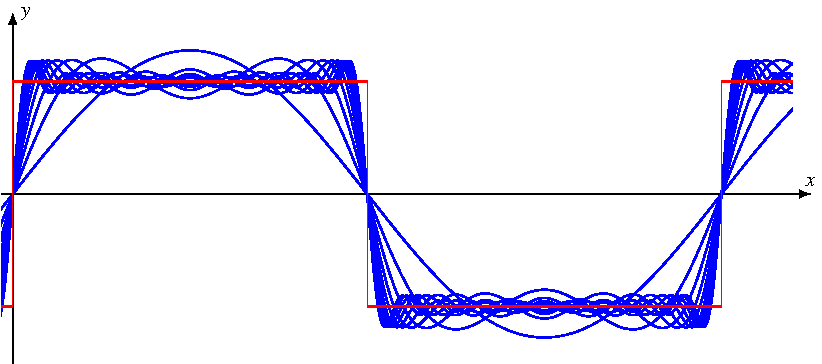
\includegraphics{chapters/010-skalarprodukt/images/fourierrechteck.pdf}
\caption{Approximation der Rechteckfunktion (rot) durch eine Folge
von Partialsummen der Fourier-Reihe.
\label{buch:skalarprodukt:fig:fourierrechteck}}
\end{figure}%
Die Supremum-Norm auf dem Raum der stetigen Funktionen hat den
Begriff der gleichmässig konvergenten Funktionenfolgen ergeben.
Cauchy-Folgen von stetigen Funktionen in der Supremum-Norm konvergieren
wieder gegen eine stetige Funktione.
Ist eine Funktion nicht stetig, lässt Sie sich im Sinne der Supremum-Norm
nicht durch stetige Funktionen approximieren.
Andererseits hat Fourier gezeigt, wie man technische wichtige Funktionen
wie die Rechteckfunktion durch trigonometrische Polynome
\begin{equation}
f_n(x)
=
\frac{4}{\pi} \sum_{k=0}^n \frac{\sin kx}{k}
=
\frac{4}{\pi} \biggl(
\sin x
+
\frac{\sin 3x}{3}
+
\frac{\sin 5x}{5}
+
\frac{\sin 7x}{7}
+
\ldots
\biggr)
\label{buch:skalarprodukt:eqn:rechteckreihe}
\end{equation}
approximieren kann.
Diese sind alle stetig und kommen der Rechteckfunktion in jedem Punkt,
in dem die Funktion stetig ist, beliebig nahe.
An den Stellen $x = n\pi$ hat die Grenzfunktion eine Sprungstelle,
die approximierenden Funktionen haben dort immer Abstand $1$
(siehe Abbildung~\ref{buch:skalarprodukt:fig:fourierrechteck}).
Die Folge ist also keine Cauchy-Folge und sie konvergiert nicht im
Sinne der Supremum-Norm.
Für solche Anwendungen muss eine besser geeignete Norm gefunden werden,
in der die Folge konvergiert.

%
% Skalarprodukt von Funktion
%
\subsubsection{Die $L^1$-Norm einer Funktion}
Die Supremum-Norm sieht nur den grössten Wert, die Konvergenz der Folge
\eqref{buch:skalarprodukt:eqn:rechteckreihe} ist aber nicht gleichmässig,
die maximale Abweichung ist immer $1$.
Gesucht ist eine Norm, die für die Folge
\eqref{buch:skalarprodukt:eqn:rechteckreihe} 
nur im Mittel eine Abweichung feststellt.
Für die Berechnung des Mittelwerts kann das Integral verwendet werden:

\begin{definition}
\label{buch:skalaprodukt:definition:l1norm}
Für eine stetige Funktion $X\to\mathbb{R}$, für die $x\mapsto |f(x)|$
integrierbar ist, heisst
\begin{equation}
\|f\|_1 = \int_X |f(x)|\,dx
\label{buch:skalarprodukt:eqn:l1norm}
\end{equation}
die {\em $L^1$-Norm} der Funktion $f$.
\end{definition}

Die $L^1$-Norm ist tatsächlich eine Norm, wir verifizieren die
definierenden Eigenschaften einer Norm.
\begin{enumerate}
\item
Definit: Sei $f$ eine stetige Funktion mit $\|f\|_1=0$
Wäre $f\ne 0$, dann gäbe es einen Punkt $x_0\in X$ mit $f(x_0) \ne 0$.
Da $f$ stetig ist, ist $f|(x)| > \frac12|f(x_0)|$ für $x$ in einer
$\delta$-Umgebung von $x_0$.
Dann folgt für die $L^1$-Norm
\begin{align*}
\|f\|_1
=
\int_X |f(x)|\,dx
\ge
\frac12 |f(x_0)| \cdot \delta 
> 0.
\end{align*}
Dies widerspricht der Annahme, dass $\|f\|_1=0$ ist, also muss $f=0$ sein.
\item
Homogeneität folgt durch direkte Rechnung
\[
\|\lambda f\|_1
=
\int_X |\lambda f(x)|\,dx
=
|\lambda|
\int_X |f(x)|\,dx
=
|\lambda| \cdot \|f\|.
\]
\item
Die Dreiecksungleichung folgt aus
\[
\|f+g\|_1
=
\int_X |f(x) + g(x)|\,dx
\le
\int_X |f(x)| + |g(x)|\,dx
=
\int_X |f(x)| + \int_X |g(x)|\,dx
=
\|f\|_1 + \|g\|_1.
\]
\end{enumerate}

Die $L^1$-Norm ist etwas ``schwächer'' als die Supremum-Norm im
folgenden Sinne.
Eine in der Supremum-Norm konvergente Funktionenfolge auf einem
kompakten Definitionsbereich $X$ ist auch in der $L^1$-Norm konvergent.
Zur Unterscheidung der verschiedenen Normen werden wir in Zukunft die
Supremum-Norm manchmal auch als $\|f\|_{\infty} = \|f\|$ schreiben.

\begin{satz}
Ist $X$ eine kompakte Teilmenge von $\mathbb{R}$ und $f_n$ eine
in der Supremum-Norm konvergente Folge stetiger Funktionen $f_n$,
dann ist $f_n$ auch in der $L^1$-Norm konvergent.
\end{satz}

\begin{proof}
Konvergenz in der Supremum-Norm bedeutet, dass für jedes $\varepsilon>0$
ein $N>0$ existiert derart, dass $|f_n(x)-f(x)|<\varepsilon$ für alle
$x\in X$ und alle $n>N$.
Für die $L^1$-Norm gilt dann
\begin{align*}
\|f_n-f\|_1
&=
\int_X |f_n(x) - f(x)|\,dx
\le
\int_X \varepsilon \,dx
=
\varepsilon \int_X \,dx
=
\varepsilon \operatorname{vol}(X).
\end{align*}
Da für einen kompakten Definitionsbereich $\operatorname{vol}(X)<\infty$
gilt, bedeutet dies, dass die $\|f_n-f\|_1\to 0$, dass also $f_n$ in
der $L^1$-Norm konvergiert.
\end{proof}

\begin{beispiel}
Die Folge $f_n(x)$ von \eqref{buch:skalarprodukt:fig:fourierrechteck}
konvergiert tatsächlich in der $L^1$-Norm auf dem Intervall $[0,2\pi]$.
Zwar ist $f_n$ nicht gleichmässig konvergent, aber fast.
Man kann zeigen, dass für jedes $\delta>0$, die Funktionen
$f_n(x)$ in Punkten $x$, die weiter als $\delta$ von den
Punkten $k\pi$ mit $k\in\mathbb{Z}$, gleichmässig konvergieren.
Innerhalb einer $\delta$-Umgebung der Vielfachen von $\pi$ ist die
$f_n(x)-f(x)$ beschränkt.
Die genaue Schranke ist nicht wichtig, wir nennen sie $M$ und bekommen
\[
|f_n(x)-f(x)|
\le M
\quad\forall x\in X.
\]
Ausserhalb einer kleinen Umgebung konvergiert die Folge gleichmässig,
zu jedem $\varepsilon>0$ gibt es also ein $N>0$ derart, dass
\[
|f_n(x)-f(x)|<\varepsilon
\]
für $x$ weiter als $\delta$ von $k\pi$ entfernt.
Für die $L^1$-Norm folgt dann
\begin{align*}
\|f_n-f\|_1
&=
\int_0^{2\pi} |f_n(x)-f(x)|\,dx
\\
&=
\int_0^\delta |f_n(x)-f(x)|\,dx
+
\int_\delta^{\pi-\delta} |f_n(x)-f(x)|\,dx
+
\int_{\pi-\delta}^{\pi+\delta} |f_n(x)-f(x)|\,dx
\\
&\qquad
+
\int_{\pi+\delta}^{2\pi-\delta} |f_n(x)-f(x)|\,dx
+
\int_{2\pi-\delta}^{2\pi} |f_n(x)-f(x)|\,dx
\\
&\le
\delta M
+
\varepsilon (\pi -2\delta)
+
2\delta M
+
\varepsilon (\pi -2\delta)
+
\delta M
\le
4\delta M + 2\pi\varepsilon
\end{align*}
für $n>N$.
Dadurch, dass man $\delta$ und $\varepsilon$ klein macht, kann man
also immer ein $N$ finden, so dass $\|f_n-f\|_1$ beliebig klein wird
für $n>N$.
Damit ist gezeigt, dass die Folge $f_n$ in der $L^1$-Norm konvergiert.
\end{beispiel}

Das Beispiel zeigt, dass die $L^1$-Norm eine schwäre Form der Konvergenz
ist, die eine erweiterte Klasse von Funktionen durch stetige Funktionen
zu approximieren erlaubt.

%
% Das $L^2$-Skalarprodukt
%
\subsubsection{Das $L^2$-Skalarprodukt}
Die $L^1$-Norm ist weniger strikt als die Supremum-Norm, aber sie ist
immer noch recht weit von der Intuition entfernt, die wir von der
Entfernungsmessung in der Geometrie haben, die von einem Skalarprodukt
herrühren.
Das Beispiel~\ref{buch:skalarprodukt:cauchyschwarz:beispiel:skalarprodukt}
weist den Weg, mit dem wir eine Norm für stetige Funktionen gewinnen
können, die von einem Skalarprodukt herkommt.

\begin{definition}
\label{buch:skalarprodukt:funktionraeume:definition:skalarprodukt}
Das {\em Skalarprodukt} stetiger Funktionen auf $X\subset \mathbb{R}$
ist definiert durch
\begin{equation}
\langle f,g\rangle
=
\int_X f(x)g(x)\,dx.
\label{buch:skalarprodukt:funktionraeume:eqn:skalarprodukt}
\end{equation}
\end{definition}

Es genügt nachzurechnen, dass $\langle f,g\rangle$ die Eigenschaften
eines Skalarproduktes hat, dann folgt die Dreiecksungleichung automatisch.
Zunächst ist klar,
dass~\eqref{buch:skalarprodukt:funktionraeume:eqn:skalarprodukt}
bilinear ist:
\begin{align*}
\langle \lambda f_1+\mu f_2,g\rangle
=
\int_X (\lambda f_1(x) + \mu f_2(x)) g(x)\,dx
&=
\lambda\int_Xf_1(x)g(x)\,dx + \mu\int_X f_2(x)g(x)\,dx
\\
&=
\lambda\langle f_1,g\rangle + \mu\langle f_2,g\rangle
\\
\langle f,\lambda g_1+\mu g_2\rangle
=
\int_X f(x)(\lambda g_1(x)+\mu g_2(x))\,dx
&=
\lambda\int_X f(x)g_1(x)\,dx + \mu\int_X f(x)g_2(x)\,dx
\\
&=
\lambda\langle f,g_1\rangle + \mu\langle f,g_2\rangle.
\end{align*}
Die Bilinearform ist aber auch positiv definit: Für eine stetige
Funktion $f(x)$ gilt
\[
\langle f,f\rangle
=
\int_X f(x)^2\,dx \ge 0.
\]
Da auch $f(x)^2$ eine stetige Funktion ist,
verschwindet das Integral genau dann, wenn $f(x)=0\;\forall x\in X$ ist.

Die zum Skalarprodukt gehörige Norm 
\[
\|f\|_2
=
\int_X |f(x)|^2\,dx
\]
heisst auch die {\em $L^2$-Norm}.

%
% Nicht kompakte Definitionsbereiche
%
\subsubsection{Nicht kompakter Definitionsbereich}
Für stetige Funktionen auf einem kompakten Definitionsbereich scheinen
die drei Normen $\|\;\cdot\;\|_\infty$, $\|\;\cdot\;\|_1$ und
$\|\;\cdot\;\|_2$ zu den gleichen Konvergenzbegriffen zu führen.
In diesem Abschnitt soll gezeigt werden, dass dies für nicht kompakte
Definitionsbereiche nicht mehr gilt.
Nicht einmal die Menge der Funktionen, die eine endliche Norm haben,
ist gleich.

\begin{beispiel}
Auf dem Definitionsbereich $X=(0,1]$ hat die Funktion
$f(x)=\log x$ endliche $L^1$-Norm aber unendliche Supremum-Norm.

\medskip
\noindent
Wegen $\lim_{x\to 0+}\log x = -\infty$ folgt $\|\log\|=\infty$.
Für die $L^1$-Norm folgt mit der Substitution $y=\log x$ und
$dy = dx/x$ oder $dx = e^y\,dy$
\begin{align*}
\|\log\|_1
&=
\int_0^1|\log x|\,dx
=
-\int_0^1\log x\,dx
=
-\int_{-\infty}^0 e^y\,dy
=
-\biggl[ e^y \biggr]_0^{-\infty}
=
1.
\end{align*}
Insbesondere ist die $L^1$-Norm beschränkt.
\end{beispiel}

\begin{beispiel}
Auf dem Definitionsbereich $X=[1,\infty)$ hat die Funktion
$f(x)=1/x$ endliche $L^2$-Norm aber unendlich $L^1$-Norm.

\medskip
\noindent
Die Integrale für die Normen ergeben:
\begin{align*}
\|f\|_1
&=
\int_1^\infty \frac{1}{x}\,dx
&
\|f\|_2^2
&=
\int_1^\infty \frac{1}{x^2}\,dx
\\
&=\biggl[\log x\biggr]_1^\infty
&
&=\biggl[-\frac{2}{x}\biggr]_1^\infty
\\
&=\infty
&
&=2.
\end{align*}
Insbesondere ist die $L^1$-Norm unbeschränkt, die $L^2$-Norm dagegen
beschränkt.
\end{beispiel}

\begin{satz}
Eine stetige Funktion auf einem beschränkten Definitionsbereich $X$
mit endlicher $L^2$-Norm hat auch endliche $L^1$-Norm.
\end{satz}

\begin{proof}[Beweis]
Aus der Cauchy-Schwarz-Ungleichung folgt
\begin{align*}
\int_X |f(x)|\,dx
&=
\langle |f|, 1\rangle
\le
\|f\|_2\cdot \|1\|_2.
\end{align*}
Nach Voraussetzung an die Funktion $f$ ist der erste Faktor beschränkt,
der zweite Faktor ist $\operatorname{vol}(X)$ und nach Voraussetzung
auch beschränkt.
\end{proof}

Die Beispiele zeigen, dass die Existenz der Normen selbst für stetige
Funktionen für nicht kompakten Definitionsbereich nicht garantiert ist.
Die Erweiterung auf nicht stetige Funktionen kann muss daher beschränkt
werden auf eine Klasse von Funktionen, für die die entsprechende Norm
existiert.
Das kann bedeuten, dass nicht alle stetigen Funktionen in Betracht 
kommen und dass neue Funktionen, die nicht stetig sind, als
Grenzwerte auftreten können.

%
% Grenzen des Riemann-Integrals
%
\subsection{Grenzen des Riemann-Integrals}
In den vorangegangenen Rechnungen sind wir immer vom Riemann-Integral
ausgegangen, welches man im Analysisunterricht als erstes kennenlernt.
Man zeigt dort, dass es für stetige Funktionen existiert und für
gleichmässig konvergente Folgen von Funktionen der Grenzwert des
Integrals mit dem Integral des Grenzwertes übereinstimmt:
\[
\int_X \lim_{n\to\infty} f_n(x)\,dx
=
\lim_{n\to\infty}
\int_X f_n(x)\,dx
\]
Der vorangegangene Abschnitt hat gezeigt, dass wir die Klasse der
Funktionen ausdehnen müssen auf Funktionen, die nicht stetig sind,
für die aber immer noch die $L^1$- oder die $L^2$-Norm existiert.
Hier zeigen sich die Schwächen des Riemann-Integrals.
In diesem Abschnitt soll an Beispielen gezeigt werden, was schief
gehen kann, und wie das Problem gelöst werden kann.

%
% Abzählbar viele Stetigkeitsstellen
%
\subsubsection{Abzählbar viele Unstetigkeitsstellen}
Wir konstruieren eine Funktionenfolge von Riemann-integrierbaren 
Funktionen, die alle das Integral $0$ haben, deren Grenzfunktion
aber nicht mehr Riemann-integrierbar ist.

Die rationalen Zahlen im Intervall $[0,1]$ sind abzählbar, d.~h.~es
gibt eine Folge $n\mapsto q_n\in[0,1]\cap\mathbb{Q}$, in der jede
rationale Zahl im Intervall vorkommt.
Aus der Folge $q_n$ konstruieren wir jetzt die Folge von Funktionen
\[
f_n(x)
=
\begin{cases} 
1&\qquad\text{$x$ ist einer der Werte $q_1,q_2,\ldots,q_n$}\\
0&\qquad\text{sonst}.
\end{cases}
\]
Die Funktion $f_n(x)$ ist also an genau $n$ Stellen von $0$ erschieden
und hat dort den Wert $1$.
Das Riemann-Integral ``sieht'' endlich viele Sprungstellen nicht,
die Funktionen $f_n$ sind also alle Riemann-integrierbar und haben
das Integral
\[
\int_0^1 f_n(x)\,dx=0.
\]
Insbesondere ist auch
\[
\lim_{n\to\infty}\int_0^1 f_n(x)\,dx = 0.
\]
Andererseits ist die Grenzfunktion
\begin{equation}
f(x)
=
\begin{cases}
1&\qquad\text{$x\in[0,1]\cap\mathbb{Q}$ ist rational}\\
0&\qquad\text{sonst, $x$ ist irrational.}
\end{cases}
\label{buch:skalarprodukt:funktionenraeume:eqn:ratfunk}
\end{equation}
Das Riemann-Integral der Funktion $f(x)$ existiert nicht.
Dazu müsste man ja für eine Unterteilung $0=x_0<x_1<\dots x_n=1$
die Riemann-Summen
\[
\overline{I}
=
\sum_{k=0}^{n-1}
(x_{k+1}-x_k) \sup_{x_k\le \xi \le x_{k+1}} f(\xi)
\qquad\text{und}\qquad
\underline{I}
=
\sum_{k=0}^{n-1}
(x_{k+1}-x_k) \inf_{x_k\le \xi \le x_{k+1}} f(\xi)
\]
berechnen, und sie müssten bei Verfeinerung der Unterteilung
gegeneinander konvergieren.
Aufgrund der Konstruktion der Funktion $f(x)$ ist aber
\[
\sup_{x_k\le \xi \le x_{k+1}} f(\xi) = 1
\qquad\text{und}\qquad
\inf_{x_k\le \xi \le x_{k+1}} f(\xi) = 0,
\]
sodass
$\overline{I}=1$ und $\underline{I}=0$ ist, ganz unabhängig von
der Unterteilung.

Der Riemannsche Integralbegriff muss also für die Zwecke der Approxmation
mit der $L^1$ oder $L^2$-Norm erweitert werden, so dass er sinnvoll mit
abzählbar vielen Unstetigkeitsstellen umgehenn kann.
Insbesondere sollte er als Integral der Funktion $f(x)$ 
von \eqref{buch:skalarprodukt:funktionenraeume:eqn:ratfunk}
den Wert $0$ liefern.

%
% Masse
%
\subsubsection{Masstheorie}
Gesucht wird also ein Integral, das für eine grössere Klasse von
Funktionen definiert ist und welches sich bezüglich Grenzwerten
besser verhält als das Riemann-Integral.
Das Integral ist nur dann nützlich, wenn es für viele Funktionen
die gleichen Werte ergibt.

Die einfachsten Funktionen, die wir integrieren wollen, sind die
{\em Indikatorfunktionen}, Funktionen, die durch eine Teilmenge
\index{Indikatorfunktion}
$A\subset X$ definiert sind durch
\[
1_A(x)
=
\begin{cases}
1&\qquad\text{für $x\in A$}\\
0&\qquad\text{sonst}.
\end{cases}
\]
Für ein Intervall der Länge $\lambda(A)$ ist
\[
\int_X 1_A(x)\,dx = \lambda(A).
\]
Für Mengen, die sich aus vielen Intervallen zusammensetzen, erwarten wir
die Summenformel
\[
A=\bigcup_{k=1}^\infty A_k,
\quad
A_k\cap A_j = \emptyset\;\forall k\ne j
\qquad\Rightarrow\qquad
\lambda(A) = \sum_{k=1}^\infty \lambda(A_k).
\]
Ausserdem sollte für eine Teilmenge $A\subset B$ der Inhalt der
Differenz $\lambda(A\setminus B)=\lambda(A)-\lambda(B)$ sein.

So entsteht eine Klasse von Mengen, denen sinnvoll ein Inhalt 
zugeordnet werden kann.
Solche Mengen heissen {\em messbar}.
Dazu gehören alle Intervalle, aber auch alle Differenzen und
abzählbaren Vereinigungen von Intervallen und messbaren Mengen
sind wieder messbar.
Die Klasse der messbaren Mengen ist also sehr gross.
Es braucht natürlich noch einiges an Arbeit, um zu zeigen, dass
eine widerspruchsfreie Definition der Funktion $\lambda(A)$
tatsächlich möglich ist, die jeder messbaren Menge einen
Inhalt zuordnet.
Eine solche Funktion heisst ein {\em Mass}, das aus der Intervalllänge
konstruierte Mass heisst auch das Lebesgue-Mass nach Henri Léon Lebesgue..
\index{Lebesgue-Mass}%
\index{Mass}%

Von besonderem Interesse sind Mengen, deren Inhalt $0$ ist.

\begin{definition}
\label{buch:skalarprodukt:funktionenraeume:definition:nullmenge}
Eine Nullmenge bezüglich des Masses $\lambda$ ist eine messbare
Menge $A$ mit Mass $\lambda(A)=0$.
\index{Nullmenge}
\end{definition}

Der Riemannsche Integralbegriff lässt bei der Bestimmung des Masses
nur endlich viele Intervalle zu. 
Die Menge $Q$ der rationalen Zahlen im Intervall $[0,1]$ ist abzählbar
unendlich.
In jeder beliebigen Umgebung einer reellen Zahl in $[0,1]$ findet man
rationale Zahlen in $Q$, eine Überdeckung der Menge der rationalen
Zahlen mit endlich vielen Intervallen enthält daher immer auch alle
reellen Zahlen, mit der möglichen Ausnahme von endlich vielen Zahlen.
Der Inhalt, den der Riemannsche Integralbegriff der Menge $Q$ zuordnen
muss, ist daher $1$.

Der neue Massbegriff erlaubt, die Menge mit abzählbar vielen messbaren
Mengen zu überdecken.
Sei $q_k$ eine Folge, die alle rationalen Zahlen in $Q$ durchläuft.
Zu jedem $k$ konstruieren wir das Intervall
\[
A_k = (q_k-\varepsilon2^{-k},q_k+\varepsilon2^{-k})
\]
mit Inhalt $\lambda(A_k) = 2\varepsilon2^{-k}$.
Es ist klar, dass die Intervalle $A_k$ die ganze Menge $Q$ überdecken,
also
\[
Q\subset \bigcup_{k=1}^\infty A_k.
\]
Der Inhalt der Menge $Q$ ist daher
\[
\lambda(Q)
\le
\sum_{k=1}^\infty \lambda(A_k)
=
\sum_{k=1}^\infty 2\varepsilon 2^{-k}
=
2\varepsilon
\sum_{k=1}^\infty 2^{-k}
=
2\varepsilon.
\]
Da $\varepsilon$ beliebig klein gewählt werden kann, folgt, dass
$\lambda(Q)=0$ sein muss.
Aus diesem Beispiel lässt sich erahnen, dass der Lebesguesche Massbegriff
mit Grenzwerten besser umgehen kann als der aus dem Riemannschen Integral
abgeleitete.

%
% Lebesgue-Integral
%
\subsubsection{Lebesgue-Integral}
Aus der Konstruktion eines Masses $\lambda$ kann jetzt die Konstruktion
eines Integrals an die Hand genommen werden.
Dazu werden Funktionen durch Stufenfunktionen approximiert, die
von der Form
\[
f(x) = \sum_{k=1}^\infty a_k 1_{A_k}(x)
\]
sind, wobei $A_k$ messbare Mengen sind.
Für solche Funktionen ist die naheliegende Definition des Integrals
\[
\int_X f(x)\,d\lambda(x)
=
\sum_{k=1}^\infty a_k \lambda(A_k).
\]
Der wesentliche Unterschied zur Riemannsschen Konstruktion ist,
dass nicht nur Intervalle zulässig sind sondern beliebige messbare Mengen.
Die Berechnung des Inhalts einer messbaren Mengen beinhaltet bereits
die Möglichkeit, Grenzwerte zu bilden.
Auch hier ist viel Arbeit notwendig um nachzuweisen, dass sich aus diesem
Ansatz ein widerspruchsfreier neuer Integralbegriff ergibt.
Das so konstruierte Integral heisst das {\em Lebesgue-Integral} und
\index{Lebesgue-Integral}%
wird zur Unterscheidung vom gewöhnlichen Riemannschen Integral und
wegen der Bedeutung des Masses $\lambda$, welches eine grosse Rolle
bei seiner Konstruktion spielt mit
\[
\int_X f(x) \,d\lambda(x)
\]
bezeichnet.

Beim Riemannschen Integral haben endliche Mengen und Mengen mit endlich
vielen Häufungspunkten Inhalt $0$.
Viele abzählbare Mengen haben dagegen positiven Inhalt.
Das Lebesguesche Mass gibt allen abzählbaren Mengen den Inhalt 0.

Unterscheiden sich zwei Funktionen $f$ und $g$ nur auf einer Nullmenge,
sagt man, sie seien {\em fast überall} gleich, geschrieben
\[
f(x) = g(x) \qquad \text{fast überall}.
\]
Zwei fast überall gleiche Funktionen haben das gleiche Integral, denn
\[
\int_X f(x)\,dx - \int_X g(x)\,dx
=
\int_X f(x)-g(x)\,dx
=
\int_X 0\,dx=0
\]
weil das Integral einer fast überall verschwindenden Funktion $0$ ist.

%
% Funktionsklassen
%
\subsubsection{Klassen von fast überall gleichen Funktionen}
Verwendet man die mit dem Lebesgque-Integral berechnete $L^1$- oder
$L^2$-Norm, dann können Funktionen nicht voneinander unterschieden werden,
die fast überall gleich sind.
Grenzwerte von Funktionenfolgen in der $L^1$- oder $L^2$-Norm sind
daher nur bis auf eine Nullmenge bestimmt.

\begin{definition}
Die Menge der Lebesgue-integrierbaren Funktionen auf dem Definitionsbereich
$X\subset\mathbb{R}$ wird mit
\[
\mathscr{L}^1(X)
=
\mathscr{L}^1_{\mathbb{R}}(X)
=
\left\{ f\colon X\to \mathbb{R}
\;\left|\;
\text{$f$ ist $\lambda$-integrierbar und $\int_X|f(x)|\,dx< \infty$}
\right.\right\}
\]
bezeichnet.
Entsprechend besteht $\mathscr{L}^2(X)$ aus den Funktionen $X\to \mathbb{R}$,
für die $|f(x)|^2$ integrierbar ist.
Sie heissen auch die {\em quadratintegrierbaren} Funktionen.
\end{definition}

Das Lebesgue-Integral kann Funktionen, die sich nur auf einer Nullmenge
verschieden sind, nicht unterscheiden. 
Daher ist es notwenig, solche Funktionen in Klassen zusammenzufassen:

\begin{definition}
Die Relation
\[
f\sim g
\qquad:\Leftrightarrow \qquad f(x) = g(x)\quad\text{fast überall}
\]
ist eine Äquivalenzrelation.
Die Menge der Äquivalenzklassen von Funktionen in $\mathscr{L}^1(X)$
bezüglich dieser Relation werden mit $L^1(X)$ bezeichnet, ebenso werden
die Äquivalenzklassen von $\mathscr{L}^2(X)$ bezüglich der Relation $\sim$
mit $L^2(X)$ bezeichnet.
\end{definition}

Mit den Funktionsklassen in $L^1(X)$ und $L^2(X)$ lässt sich genau
so rechnen, wie man es sicht gewohnt ist.
Für die Summe von Funktionen $f_1\sim f_2$ und $g_1\sim g_2$ gilt
\[
\left.
\begin{aligned}
f_1(x)&=f_2(x)&&\text{fast überall}\\
g_1(x)&=g_2(x)&&\text{fast überall}\\
\end{aligned}
\quad
\right\}
\qquad
\Rightarrow
\qquad
f_1(x)+g_1(x) = f_2(x)+g_2(x)\quad\text{fast überall},
\]
denn die Menge, auf der sich $f_1+f_2$ und $g_1+g_2$ unterscheiden
ist höchstens die Vereinigung der Mengen, auf denen sich $f_1$ und 
$f_2$ bzw.~$g_1$ und $g_2$ unterscheiden.
Die Vereinigung von Nullmengen ist aber wieder eine Nullmenge.

%
% Lebesgue-Integral
%
\subsubsection{Dominierte Konvergenz}
Die Entwicklung des Lebesgueschen Integrallbegriffs war motiviert
vom Wunsch, ein Integral zu erhalten, welches sich bezüglich
Konvergenz von Funktionenfolgen besser verhält.
Tatsächlich liefert die Theorie den folgenden zentralen Satz.

\begin{satz}[Dominierte Konvergenz]
\label{buch:skalarprodukt:satz:dominierte-konvergenz}
Sei $f_n$ eine auf dem Definitionsbereich $X$ punktweise konvergente
Folge Lebesgue-integrierbarer Funktionen mit Grenzfunktion 
\[
f(x) = \lim_{n\to \infty} f_n(x).
\]
Sei ausserdem $g$ eine Lebesgue-integrierbare Funktion mit
$|f_n(x)|<g(x)$ für alle $x\in X$.
Dann ist $f$ Lebesgue-integrierbar und es gilt
\[
\lim_{n\to\infty} \int_X f(x)\,d\lambda(x)
=
\int_X f(x)\,d\lambda(x)
\]
\end{satz}

Der Satz der dominierten Konvergenz von Lebesgue ersetzt also die
Bedingung der gleichmässigen Konvergenz, die beim Riemann-Integral
erfolgreich war, durch die viel schächere Bedingung, dass alle
Funktionen unterhalb einer gemeinsamen integrierbaren Funktion bleiben.
Dadurch wird verhindert, dass die Funktionen $f_n$ nach $\infty$
``ausbrechen'' kann und gegen eine Funktion konvergieren, die nicht
mehr integrierbar ist.


%
% Berechnung von Lebesgue-Integralen
%
\subsubsection{Berechnung von Lebesgue-Integralen}
Das Lebesque-Integral löst also die technischen Probleme, die das
Riemann-Integral manchmal bei Funktionenfolgen hat, die gegen ein
Grenzfunktion konvergieren, der man ein sinnvolles Integral im
Lebesgueschen Sinnen zuordnen kann.
Doch wie berechnet man ein Lebesgue-Integral?

Stetige Funktionen lassen sich beliebig genau durch Treppenfunktionen
approximieren.
Die Konvergenz des Lebesgue-Integrals für solche Funktionenfolgen
garantiert daher, dass das Lebesgue-Integral für stetige
Funktionen mit dem Riemann-Integral übereinstimmt.
Insbesondere braucht es keinen neuen Formalismus für die 
Berechnung von Integralen.
Auch für Funktionen, die an höchstens endlich vielen Stellen unstetig
sind, stimmt das Riemann-Integral mit dem Lebesgue-Integral überein.

Man soll sich daher das Lebesgue-Integral vor allem als eine 
Erweiterung des Integrals auf Funktionen vorstellen, die als Grenzwerte
von Folgen stetiger Funktionen im Sinne der $L^1$- oder der $L^2$-Norm
auftreten können.
Stetigkeit kann dabei verloren gehen, aber Konvergenzeigenschaften
wie die dominierte Konvergenz von
Satz~\ref{buch:skalarprodukt:satz:dominierte-konvergenz}
bleiben erhalten.




%
% 4-hilbertraum.tex
%
% (c) 2022 Prof Dr Andreas Müller, OST Ostschweizer Fachhochschule
%
\section{Hilbert-Raum
\label{buch:skalarprodukt:section:hilbertraum}}
\kopfrechts{Hilbert-Raum}
Ein Skalarprodukt stattet einen Vektorraum mit einer Norm aus.
Es ermöglicht auch, orthonormierte Vektoren zu finden.
In endlichdimensionalen Vektorräumen können so besonders nützliche
Basen konstruiert werden.
In den Funktionenräumen von
Abschnitt~\ref{buch:skalarprodukt:section:funktionenraeume},
die unendlichdimensional sind, kann der Orthonormalisierungsprozess
ohne Ende weitergeführt werden.
Im Gegensatz zu einem endlichdimensionalen Vektorraum bilden diese
orthonormierten Vektoren keine Basis, denn nicht jeder Vektor lässt
sich als Linearkombination schreiben.
Dies wird erst mit Hilfe von Reihenentwicklungen möglich, doch dazu
müssen Fragen der Konvergenz solcher Reihen geklärt werden.
Der in diesem Abschnitt eingeführte Begriff des Hilbert-Raumes tut dies.

%
% Prähilbertraum
%
\subsection{Prähilbertraum}
Die Funktionenräume, in denen wir harmonische Analysis betreiben wollen,
zeichnen sich durch das Vorhandensein eines Skalarproduktes aus.
Wir fassen diese Eigenaschaften im Begriff des Prähilbertraumes
zusammen.

\begin{definition}
Ein reeller Prähilbertraum ist ein reller Vektorraum mit einem
(reellen) Skalarprodukt.
\index{Prähilbertraum}%
Eine komplexer Prähilbertraum ist ein komplexer Vektorraum mit einem
sesquilinearen Skalarprodukt.
\end{definition}

\begin{beispiel}
Der endlichdimensionale reelle Vektorraum $\mathbb{R}^n$ ist ein
reller Prähilbertraum mit dem Skalarprodukt
\[
\langle u,v\rangle
=
\sum_{i=1}^n u_iv_i
\]
für Vektoren $u,v\in\mathbb{R}^n$.
\end{beispiel}

\begin{beispiel}
Der endlichedimensionale komplexe Vektorrau $\mathbb{C}$ ist ein
komplexer Prähilbertraum mit dem Skalarprodukt
\[
\langle u,v\rangle
=
\sum_{i=1}^n \overline{u}_iv_i
\]
für Vektoren $u,v\in\mathbb{C}^n$.
\end{beispiel}

Die Skalarprodukte in den Beispielen sind nicht die einzig möglichen
Skalarprodukte.
Alternative Skalarprodukte auf einem reellen Prähilbertraum können 
durch eine beliebige positiv definite Matrix $A$ durch
\[
\langle u,v\rangle_A
=
\sum_{i,j=1}^n u_ia_{ij}v_j
\]
definiert werden.
Wir schreiben die aus $\langle\;,\;\rangle_A$ abgeleitete Norm mit
$\normfunc_A$.
Solange unser primäres Interesse der Approximation von Funktionen gilt,
kommt es vor allem darauf an, dass die Norm, die aus dem Skalarprodukt
abgeleitet wird, zu den gleichen konvergenten Folgen führen.
Die Funktion $u\mapsto \|u\|_A$ ist stetig, sie hat daher auf der
Einheitskugel des Prähilbertraumes ein Maximum und eine Minimum,
welches wir mit $M$ bzw.~$m$ bezeichen.
Dann folgt, dass
\[
m\|u\|\le \|u\|_A\le M\|u\|
\]
für beliebige Vektoren $u\in\mathbb{R}^n$.
Daraus kann man jetzt ableiten, dass die beiden Normen $\normfunc$
und $\normfunc_A$ auf die gleichen Cauchy-Folgen und die gleichen
konvergenten Folgen führen.
Wir zeigen dies für Cauchy-Folgen:
\begin{enumerate}
\item
Sei $u_k$ eine Cauchy-Folge bezüglich der Norm $\normfunc$,
und $\varepsilon>0$.
Wir müssen zeigen, dass $u_k$ auch eine Cauchy-Folge ist bezüglich
der Norm $\normfunc_A$.
Da $u_k$ eine Cauchy-Folge bezüglich der Norm $\normfunc$ ist,
gibt es ein $N>0$ derart, dass
$\|u_k-u_l\|<\varepsilon/M$ für $k,l>N$.
Dann folgt aber
\[
\|u_k-u_l\|_A
\le
M\|u_k-u_l\|
<
M\frac{\varepsilon}{M}
=
\varepsilon
\]
für $k,l>N$.
Somit ist $u_k$ eine Cauchy-Folge bezüglich der Norm $\normfunc_A$.
\item
Ist umgekehrt  $u_k$ eine Cauchy-Folge bezüglich der Norm $\|\,\cdot\,\|_A$,
dann gibt es ein $N>0$ derart, dass $\|u_k-u_l\|_A<m\varepsilon$ ist für
$k,l>N$.
Dann folgt
\[
m\|u_k-u_l\|\le \|u_k-u_l\|_A < m\varepsilon
\qquad\Rightarrow\qquad \|u_k-u_l\|<\varepsilon
\]
für $k,l>N$, also ist $u_k$ auch eine Cauchy-Folge bezüglich der Norm
$\|\,\cdot\,\|$.
\end{enumerate}
In einem endlichdimensionalen Prähilbertraum hat die Wahl des Skalarproduktes
keinen Einfluss darauf, ob eine Folge eine Cauchy-Folge ist oder nicht.
Orthonormierte Vektoren werden natürlich im Allgemeinen nicht mehr
orthonormiert, dies ist jedoch ein Aspekt, dem wir uns erst später
zuwenden werden.

%
% Orthonormierte Vektoren
%
\subsection{Orthonormierte Vektoren in einem Prähilbertraum}
Der Gram-Schmidt-Orthogonalisierungsprozess kann auf eine beliebige
\index{Gram-Schmidt}%
linear unabhängige Menge von Vektoren in einem Prähilbertraum angewendet
werden.
Aus den linear unabhängigen Vektoren $a_1,a_2,\dots$ werden die
orthonormierten Vektoren
\begin{align*}
b_1
&=
\frac{a_1}{\|a_1\|}
\\
b_2
&=
\frac{
a_2 - \langle b_1,a_2\rangle b_1
}{
\|a_2 - \langle b_1,a_2\rangle b_1\|
}
\\
&\phantom{i}\vdots
\\
b_n
&=
\frac{\displaystyle
a_n - \sum_{k=1}^{n-1} \langle b_k,a_n\rangle b_k
}{\displaystyle
\biggl\|a_n - \sum_{k=1}^{n-1} \langle b_k,a_n\rangle b_k\biggr\|
}.
\end{align*}

In einem endlichdimensionalen Vektorraum der Dimension $n$ bricht
der Prozess ab, sobald eine orthonormierte Basis $b_1,\dots,b_n$
aus $n$ Vektoren gefunden wurde.
Jeder andere Vektor $v$ lässt sich dann als Linearkombination
\begin{equation}
v
=
\langle b_1,v\rangle b_1 + \langle b_2,v\rangle b_2 + \dots
=
\sum_{k=1}^n \langle b_1,v\rangle b_1
\label{buch:skalarprodukt:hilbertraum:synthese}
\end{equation}
schreiben.
Da die Summe auf der rechten Seite endlich ist, entstehen keine
Bedenken bezüglich Konvergenz, wie das bei einer unendlichen
Reihe der Fall wäre.

%
% Vollständigkeit
%
\subsection{Vollständigkeit}
In einem unendlichdimensionalen Prähilbertraum bricht der
Orthogonalisierungsprozess nicht ab, es gibt immer noch einen
linear unabhängigen Vektor, der nicht in dem von den bereits
gefundenen Vektoren aufgespannten Raum liegt.
Die Summe~\ref{buch:skalarprodukt:hilbertraum:synthese} wird dann
eine unendliche Summe, die nur im Sinne eines Grenzwertes der
Partialsummenfolge
\begin{equation*}
s_n = \sum_{k=1}^n \langle b_k,v\rangle b_k
\end{equation*}
ausgewertet werden kann.
Man darf zwar aufgrund der Konstruktion aus $v$ davon ausgehen,
dass $s_n$ gegen $v$ konvergiert,
aber für eine beliebige Folge von Koeffizienten $c_k$ ist nicht
garantiert, dass die Summe
\[
\sum_{k=1}^\infty c_kb_k
=
\lim_{n\to\infty} \sum_{k=1}^n c_kb_k
\]
einen Grenzwert hat.
Ein nützliche Theorie kann nur entstehen, wenn gefordert wird,
dass jede Cauchy-Folge des Prähilbertraums tatschächlich konvergiert.

\begin{definition}
Ein Prähilbertraum heisst {\em Hilbert-Raum}, wenn er vollständig ist.
\end{definition}

Endlichdimensionale Vektorräume über sind automatisch vollständig,
da gibt es also gar keinen Unterschied zwischen Prähilbertraum und
Hilbert-Raum.
Das folgende Beispiel zeigt, dass dies für unendlichdimensionale
Hilbert-Räume nicht mehr zutrifft.

\begin{beispiel}
\label{buch:skalarprodukt:hilbertraum:bsp:sinreihe}
Der Funktionenraum
\(
C_{\mathbb{R}}([-\pi,\pi])
\)
der stetigen Funktionen auf dem Intervall $[-\pi,\pi]$ wird mit
dem Skalarprodukt
\[
\langle f,g\rangle
=
\int_{-\pi}^\pi f(x)g(x)\,dx
\]
zu einem Prähilbert-Raum.
Die Summanden der Reihe~\eqref{buch:skalarprodukt:eqn:rechteckreihe} 
sind Sinus-Funktionen, von denen wir später zeigen werden, dass sie
orthogonal sind.
Seien $s_n(x)$ die Partialsummen der Reihe, also
\begin{equation}
s_n(x) = \frac{4}{\pi}\sum_{k=0}^n \frac{\sin (2k+1)x}{2k+1},
\label{buch:skalarprodukt:hilbertraum:eqn:sn}
\end{equation}
dann kann man auch die Norm $\|s_n-s_m\|$, es gilt nämlich
\begin{equation}
\|s_n-s_m\|
=
\biggl\|
\frac{4}{\pi}
\sum_{k=m}^n \frac{\sin (2k+1)x}{2k+1}
\biggr\|,
\label{buch:skalarprodukt:hilbertraum:eqn:snsm}
\end{equation}
wobei wir $n>m$ angenommen haben, was wir ohne Beschränkung der 
Allgemeinheit tun dürfen.
Die Norm eines einzeln Terms ist
\begin{align}
\|\sin rx\|^2
&=
\int_{-\pi}^\pi \sin^2 rx\,dx
=
\int_{-\pi}^\pi \frac12 - \frac{\cos rx}{2}\,dx
=
\int_{-\pi}^\pi \frac12\,dx - \int_{-\pi}^\pi \frac{\cos rx}{2}\,dx.
\notag
\intertext{Der zweite Term ist ein Integral über eine Periode des
Integranden und verschindet daher.
Der erste Term ergibt daher}
\|\sin rx\|^2
&= \pi.
\intertext{Für die Terme der Summe
\eqref{buch:skalarprodukt:hilbertraum:eqn:sn}
folgt daher}
\biggl\|
\frac{\sin{2k+1}x}{2k+1}
\biggr\|^2
&=
\frac{\pi}{(2k+1)^2}.
\notag
\intertext{Für die Differenz
\eqref{buch:skalarprodukt:hilbertraum:eqn:snsm} finden wir daher}
\|s_n-s_m\|^2
\notag
&=
\frac{16}{\pi^2}
\sum_{k=m}^m \frac{\pi}{(2k+1)^2}
=
\frac{16}{\pi}
\sum_{k=m}^m \frac{1}{(2k+1)^2}.
\label{buch:skalarprodukt:hilbertraum:eqn:bsprest}
\end{align}
Da aus dem Analysisunterricht bekannt ist, dass die Reihe $\sum_k\frac1{k^2}$
konvergiert, kann die rechte Seite von 
\eqref{buch:skalarprodukt:hilbertraum:eqn:bsprest}
beliebig klein gemacht werden, die 
Reihe~\eqref{buch:skalarprodukt:eqn:rechteckreihe} 
ist also eine Cauchy-Folge im Prähilbertraum $C_{\mathbb{R}}([-\pi,\pi])$.
Die Grenzfunktion ist die Rechteckfunktion von
Abbildung~\ref{buch:skalarprodukt:fig:fourierrechteck}, sie ist nicht
stetig.
Wir haben also eine Cauchy-Folge im Prähilbertraum 
$C_{\mathbb{R}}([-\pi,\pi])$ gefunden, die darin nicht konvergiert.
\end{beispiel}

%
% Hilbert-Basis
%
\subsection{Hilbert-Basis}
Sei jetzt $H$ ein Hilbert-Raum.
Führt man wieder die Konstruktion einer orthonormierten Basis durch,
entsteht eine Menge $\mathcal{B}=\{b_1,b_2,\dots\}$ orthonormierter
Vektoren.
In einem unendlichdimensionalen Hilbert-Raum ist $\mathcal{B}$ eine
undendliche Menge.
Die Vollständigkeit des Hilbert-Raumes garantiert, dass jede
Cauchy-Folge konvergiert, insbesondere können wir zu jedem beliebigen
Vektor $v$ die Koeffizienten $c_k=\langle b_k,v \rangle$ bestimmen
und versuchen, mit der
Summe~\eqref{buch:skalarprodukt:hilbertraum:synthese}
den Vektor zurückzugewinnen.
Vollständigkeit garantiert zwar die Konvergenz gegen einen Grenzwert
\[
v_0 = \sum_{k=1}^\infty c_k b_k,
\]
aber es gibt keine Garantie, dass $v=v_0$ ist.

\begin{beispiel}
Die Funktionen
\[
b_k(x) = \sin (2k+1)x
\qquad\text{mit}\quad
k\in \mathbb{N}
\]
wurden in Beispiel~\ref{buch:skalarprodukt:hilbertraum:bsp:sinreihe}
die Rechteckfunktion synthetisiert.
Doch reichen diese Funktionen nicht aus, um alle Funktionen auf
dem Intervall $[-\pi,\pi]$ zu synthetisieren.

Für die konstante Funktion $v(x)$ sind die Koeffizienten
\[
\langle v,b_k\rangle
=
\int_{-\pi}^\pi v(x)b_k(x)\,dx
=
\int_{-\pi}^\pi \sin (2k+1)x\,dx
=
0,
\]
die Summe
\[
v_0
=
\sum_{k=0}^\infty
c_k
b_k(x)
=
0
\]
verschwindet also, $v\ne v_0$.
\end{beispiel}

Wir berechnen das Skalarprodukt 
\[
\langle v-v_0,b_k\rangle
=
\langle v,b_k\rangle
-
\biggl\langle \sum_{l=1}^\infty c_lb_l,b_k\biggr\rangle
=
c_k - \sum_{l=1}^\infty c_l\langle b_l,b_k\rangle
=
c_k - \sum_{l=1}^\infty c_l\delta_{lk}
=
c_k-c_k=0.
\]
Der Vektor $v-v_0$ muss also orthogonal sein zu allen Vektoren
$b_k$.
Die Menge der Vektoren $b_k$ kann also vergrössert werden um einen
weiteren Vektor, der zu allen vorhandenen Vektoren orthogonal ist.

\begin{satz}
Eine Menge von orthogonalen Vektoren in einem Prähilbertraum ist linear 
unabhängig.
\end{satz}

\begin{proof}[Beweis]
Angenommen, die orthogonalen Vektoren  $a_1,\dots,a_n$ sind linear
abhängig.
Dann gibt es Zahlen $\lambda_i$, die nicht alle $=0$ sind und derart,
dass
\[
\sum_{k=1}^n \lambda_ka_k
=
\lambda_1 a_1 + \ldots + \lambda_n a_n
=
0.
\]
Das Skalarprodukt mit $a_k$ ergibt
\[
0
=
\langle a_k,\lambda_1a_1 +\ldots + \lambda_na_n\rangle
=
\lambda_1
\langle a_k,a_1\rangle
+
\ldots
+
\lambda_n
\langle a_k,a_n\rangle
=
\lambda_k \|a_k\|^2
\]
für alle $k=1,\dots,n$.
Da die Vektoren $a_k\ne 0$ sind folgt, dass $\lambda_k=0$ sein muss
für alle $k=1,\dots,n$, im Widerspruch zur Voraussetzung, dass die
$\lambda_k$ nicht alle verschwinden.
Der Widerspruch zeigt, dass die Annahme der linearen Abhängigkeit
falsch ist.
\end{proof}

In einem endlichdimensionalen Prähilbertraum findet man immer eine
orthonormierte Basis, aus der sich jeder Vektor linear kombinieren
lässt.
In einem unendlichdimensionalen Raum muss dieser Begriff etwas 
erweitert werden.

\begin{definition}
Eine {\em Hilbert-Basis} des Hilbert-Raumes $H$ ist eine Menge von orthonormalen
\index{Hilbert-Basis}%
Vektoren $b_k\in H$, $k\in \mathbb{N}$ derart, für jeden Vektor $v\in H$
die Reihe 
\[
\sum_{k\in\mathbb{N}} \langle b_k,v\rangle b_k
\]
konvergiert und die Summe $v$ hat.
\end{definition}

Auf eine Hilbert-Basis ist die Inuition anwendbar, die man von 
einer orthonormierten Basis eines endlichdimensionalen Prählibertraumes
hat.

\begin{definition}
\index{separabel}%
Ein Hilbert-Raum, der eine Hilbert-Basis besitzt, heisst {\em separabel}.
\end{definition}

Nicht separable Hilbert-Räume sind deutlich grösser.
In einem nicht separable Hilbert-Raum ist es nicht möglich, alle Vektoren
aus einer Folge von orthonormierten Vektoren linear zu kombinieren.
Dies verträgt sich nicht mit der Intuition, die in endlichdimensionalen
Vektorräumen entstanden ist.
Separabilität ist eine Art ``Endlichkeitseigenschaft''.
Man findet sie zum Beispiel bei den $L^2$-Räumen mit kompaktem
Definitionsgebiet.
Kompaktheit kann als eine topologische
Endlichkeitseigenschaft angesehen werden.
Es lassen sich aber auch nicht separable Hilbert-Räume konstruieren,
zum Beispiel sogenannte fastperiodische Funktionen.
\index{fastperiodische Funktionen}%
Für unsere Anwendungen sind nicht separable Hilbert-Räume jedoch nicht
notwendig und wir können im folgenden annehmen, dass alle Hilbert-Räume
separabel sind und somit eine Hilbert-Basis haben.

%
% Der Hilbert-Raum $l^2$
%
\subsection{Der Hilbert-Raum $l^2$}
Die abstrakte Definition eines separablen Hilbert-Raumes suggeriert,
dass es sehr viele verschiedene Hilbert-Räume geben könnte.
Dem ist aber nicht so, ein Hilbert-Raum ist eine ziemlich starre Struktur.
In diesem Abschnitt konstrieren wir zunächst den besonders übersichtlichen
separablen Hilbert-Raum $l^2$ und zeigen anschliessend, dass sich jeder
separable Hilbert-Raum isometrisch auf $l^2$ abbilden lässt.

\begin{satz}
Der Vektorraum der unendlichen Folgen
\[
l^2_{\mathbb{R}}
=
\biggl\{
(x_0,x_1,\dots)
\in
\mathbb{R}^{\mathbb{N}}
\,\bigg|\,
\sum_{i=0}^\infty x_i^2<\infty\biggr\}
\}
\]
mit dem Skalarprodukt
\[
\langle x,y\rangle_2
=
\sum_{k=0}^\infty x_ky_k
\]
ist ein separabler Hilbert-Raum.
\end{satz}

\begin{proof}[Beweis]
Die Standardbasis des Vektorraums $l^2$ besteht aus den Vektoren $e_i$
mit $i\in\mathbb{N}$ mit 
\begin{align*}
e_0 &= (1,0,0,0,\dots)
\\
e_1 &= (0,1,0,0,\dots)
\\
e_2 &= (0,1,0,0,\dots)
\\  &\;\vdots
\end{align*}
Es ist klar, dass die Vektoren $e_i$ orthonormiert sind.
Wir müssen uns überlegen, dass jede Folge in $l^2$ durch Linearkombinationen
approximiert werden kann.
Wäre das nicht so, dann gäbe es einen von $0$ verschiedenen
Vektor $v=(v_0,v_1,v_2,\dots)\in l^2$, der auf allen Vektoren $e_i$
orthogonal ist.
Dann wäre aber $0=\langle v,e_i\rangle = v_i$, d.~h.~Vektor $v$ ist der
Nullvektor.
Dieser Widerspruch zeigt, dass die Vektoren $e_i$ eine Hilbert-Basis
bilden.
\end{proof}

Der Hilbert-Raum $l^2$ ist die einfachste, direkte Verallgemeinerung der
endlichdimensionalen Hilbert-Raume $\mathbb{R}^n$ mit dem Standardskalarprodukt.
Er ist aber auch der ``einzige'' separable Hilbert-Raum, alle Hilbert-Räume
lassen sich isometrisch auf $l^2$ abbilden.

\begin{satz}
\label{buch:skalarprodukt:hilbertraum:satz:phil2}
Ist $H$ ein separabler Hilbert-Raum, dann gibt es eine isometrische
lineare Abbildung $\varphi\colon H\to l^2$.
\end{satz}

\begin{proof}[Beweis]
Da $H$ separabel ist, gibt es eine Hilbert-Basis $b_0,b_1,b_2,\ldots\in H$
und $v$ ein beliebiger Vektor mit der Darstellung
\[
v = \sum_{k=0}^\infty c_kb_k.
\]
Das Skalarprodukt mit $b_k$ ist
\[
\langle b_i,v\rangle
=
\biggl\langle b_i,\sum_{k=0}^\infty c_kb_k\biggr\rangle
=
\sum_{k=0}^\infty c_k \underbrace{\langle b_i,b_k\rangle}_{\delta_{ik}}
=
c_i.
\]
Die Abbildung
\[
\varphi\colon H \to l^2
:
v \mapsto (\langle b_0,v\rangle,\langle b_1,v\rangle,\langle b_2,v\rangle,\dots)
=
(c_0,c_1,c_2,\dots)=c\in l^2
\]
ist linear und umkehrbar durch die Abbildung
\[
\varphi^{-1} \colon l^2 \to H
:
(c_0,c_1,c_2,\dots) \mapsto \sum_{k=0}^\infty c_k b_k.
\]
Die Norm von $v$ ist
\[
\|v\|^2
=
\biggl\|
\sum_{k=0}^\infty c_k b_k
\biggr\|^2
=
\sum_{k=0}^\infty c_k^2
=
\|c\|_2^2.
\qedhere
\]
\end{proof}

Man verliert also nichts, wenn man statt im Hilbert-Raum $H$ im
Hilbert-Raum $l^2$ rechnet.
Die später zu besprechende Fourier-Transformation ist genau
so eine Abbildung $\varphi$ wie in
Satz~\ref{buch:skalarprodukt:hilbertraum:satz:phil2}, wenn 
trigonometrische Funktionen als Basisfunktionen des Raumes
$L^2([-\pi,\pi])$ verwendet werden.
Die Tatsache, dass die Abbildung eine Isometrie ist, hat einen
speziellen Namen.

\begin{definition}
\label{buch:skalarprodukt:hilbertraum:def:parseval}
Die Identität
\[
\|v\|^2 = \|\varphi(v)\|_2^2
\]
heisst {\em Parseval-Gleichung}.
Aus der Polaridentität folgt dann auch die
{\em Parseval-Plancherel-Formel}
\[
\langle u,v\rangle_H
=
\langle\varphi(u),\varphi(v)\rangle_2
=
\sum_{k=0}^\infty
\langle b_k,u\rangle
\langle b_k,v\rangle.
\]
\end{definition}

Die endlichdimensionalen Hilbert-Räume können auf
natürliche Art in $l^2$ eingebettet werden, indem die Koordinaten
eines $n$-dimensionalen Vektors auf die ersten $n$-Komponenten der
Folge in $l^2$ abgebildet werden.
Aus dieser Idee lässt sich auch ein Prähilbertraum konstruieren,
in dem einfacher gerechnet werden kann.

\begin{definition}
\label{buch:skalarprodukt:hilbertraum:def:l0}
Sei 
\[
l_0
=
\{
x\in \mathbb{R}^{\mathbb{N}}
\mid
\text{$x_k\ne 0$ nur für endlich viele $k$}
\}
\]
der Vektorraum der Folgen, die nur endlich viele nicht verschwindende
Folgenglieder haben.
Die Standardbasisvektoren von $l^2$ sind alle in $l_0$.
\end{definition}

Da die Norm eines Elementes $x\in l_0$ eine endliche Summe ist,
ist $x\in l^2$ und damit $l_0\subset l^2$.
Jeder Vektor $v\in l^2$ kann aber beliebig genau durch einen Vektor
in $l_0$ approximiert werden.
Dazu konstruiert man die Folge
\bgroup
\def\el#1{\phantom{v_0}\llap{#1}}
\begin{align*}
x_0 &= (v_0,\el{0},\el{0},\el{0},\el{0},\dots) \in l_0\\
x_1 &= (v_0,v_1,\el{0},\el{0},\el{0},\dots) \in l_0\\
x_2 &= (v_0,v_1,v_2,\el{0},\el{0},\dots) \in l_0\\
x_3 &= (v_0,v_1,v_2,v_3,\el{0},\dots) \in l_0\\
    &\;\vdots
\end{align*}
\egroup
Die Differenz $x_n-v$ hat die Norm
\[
\|x_n-v\|^2
=
\sum_{k=n+1}^\infty v_k^2,
\]
die für $n\to\infty$ gegen $0$ geht.
Da es in $l^2$ Vektoren gibt, die nicht in $l_0$ drin sind, zeigt
dies, dass $l_0$ kein Hilbert-Raum ist, dass aber die Vervollständigung
von $l_0$ der Hilbert-Raum $l^2$ ist.

Der Prähilbert-Raum rechtfertigt, dass man in Anwendungen im Sinne
einer Approximation mit endlich vielen der Koeffizienten $c_k$
rechnen kann.
Im Kontext der Fourier-Theorie sind dies
die trigonometrischen Polynome, mit denen sich jede periodische
Funktion approximieren lässt.

%
% Der Hilbert-Raum $L^2$
%
\subsection{Der Hilbert-Raum $L^2$}
Der Vektorraum der stetigen Funktionen auf dem Intervall $[-\pi,\pi]$
mit dem bekannten Skalarprodukt ist ein Prähilbertraum.
Wir werden später zeigen, dass die Funktionen
\[
1, \cos kx \quad\text{und}\quad \sin kx
\qquad \text{mit $k\in\mathbb{N}$ und $ k\ge 1$}
\]
orthogonal sind bezüglich dieses Skalarproduktes.
Es wird sich zeigen, dass diese Funktionen nach geeigneter Normierung
eine Hilbert-Basis bilden von $L^2$ bilden.
Die in Satz~\ref{buch:skalarprodukt:hilbertraum:satz:phil2}
konstruierte Abbildung bezeichnen wir mit $\mathscr{F}:L^2([-\pi,\pi])\to l^2$.
Die Parseval-Plancherel-Formel besagt dann, dass man das Skalarprodukt
von Funktionen auch durch das Skalarprodukt der zugehörigen
Fourier-Koeffizienten berechnen kann:
\[
\langle f,g\rangle_{L^2{[-\pi,\pi]}}
=
\langle \mathscr{F}f,\mathscr{F}g\rangle_{l^2}.
\]
Die Fourier-Transformation formalisiert also die Erkenntnis, dass
man alle Fragen, die man mit Skalarprodukten beantworten kann, statt
mit Funktionen auch mit Skalarprodukten von Fourier-Koeffizienten
finden kann.

%
% Der Darstellungssatz von Riesz
%
\subsection{Der Darstellungssatz von Riesz}
Eine Linearform $l(x)$ auf dem Vektorraum $\mathbb{R}^n$ ist gegeben durch
die Werte $l(e_i)$ auf den Standardbasisvektoren.
Der Wert von auf $x=x_1e_1+\dots+x_ne_n$ ist dann
\[
l(x)
=
x_1l(e_1)+\dots+x_nl(e_n)
=
\begin{pmatrix}
l(e_1)\\\vdots\\l(e_n)
\end{pmatrix}
\cdot
\begin{pmatrix}
x_1\\\vdots\\x_n
\end{pmatrix}.
\]
Insbesondere lässt sich jede Linearform als Skalarprodukt mit einem 
geeigneten Vektor geschrieben werden.
Diese Eigenschaft gilt auch in einem Hilbert-Raum.

\begin{satz}[Riesz]
\label{buch:skalarprodukt:hilbertraum:satz:riesz}
Sei $H$ ein Hilbert-Raum und $l\colon H\to\mathbb{R}$ eine stetige
Linearform.
Dann gibt es eine $v\in H$ derart, dass $l(x) = \langle v,x\rangle$.
\end{satz}

Der Beweis dieser Eigenschaft kann man zum Beispiel in \cite{buch:wavelets}
finden.
Der Satz gilt natürlich auch in einem komplexen Hilbert-Raum.




%
% 5-sobolevraum.tex
%
% (c) 2022 Prof Dr Andreas Müller, OST Ostschweizer Fachhochschule
%
\section{Sobolev-Räume
\label{buch:skalarprodukt:section:sobolev}}
\kopfrechts{Sobolev-Räume}
Im Beispiel~\ref{buch:skalarprodukt:hilbertraum:bsp:sinreihe} haben 
wir eine Reihe kennengelernt, deren Partialsummen alle stetig sind,
da sie trigonometrische Polynome sind.
Doch die Grenzfunktion ist die Rechteckfunktion, die ganz offensichtlich
nicht stetig sind.
Die Norm des Hilbert-Raums $L^2$ ist offenbar nicht stark genug, die
Stetigkeit der Grenzfunktion sicherzustellen.

%
% tikztemplate.tex -- template for standalon tikz images
%
% (c) 2021 Prof Dr Andreas Müller, OST Ostschweizer Fachhochschule
%
\documentclass[tikz]{standalone}
\usepackage{amsmath}
\usepackage{times}
\usepackage{txfonts}
\usepackage{pgfplots}
\usepackage{csvsimple}
\usepackage{ifthen}
\usetikzlibrary{arrows,intersections,math}
\begin{document}
\def\skala{1}
\newboolean{draft}
\setboolean{draft}{false}
\begin{tikzpicture}[>=latex,thick,scale=\skala]

% add image content here
\def\s{12/(2*3.14159)}
\def\punkt#1#2{({(#1)*\s},{(#2)*\s})}

\draw[->] (-0.6,0) -- (13.2,0) coordinate[label={$x$}];
\draw[->] (0,{-1.72*\s}) -- (0,{1.8*\s}) coordinate[label={right:$y$}];

\begin{scope}
\clip (-0.6,{-1.8*\s}) rectangle (13.0,{1.8*\s});
\draw[color=blue] plot[domain=-20:420,samples=100]
	({(\x/360)*\s*2*3.14159},{(4/3.14159)*sin(\x)*\s});
\draw[color=blue] plot[domain=-20:420,samples=1000]
	({(\x/360)*\s*2*3.14159},{(4/3.14159)*(sin(\x)-sin(3*\x)/3)*\s});
\ifthenelse{\boolean{draft}}{}{
\draw[color=blue] plot[domain=-20:420,samples=1000]
	({(\x/360)*\s*2*3.14159},{(4/3.14159)*(sin(\x)-sin(3*\x)/(3*3)+sin(5*\x)/(5*5))*\s});
\draw[color=blue] plot[domain=-20:420,samples=1000]
	({(\x/360)*\s*2*3.14159},{(4/3.14159)*(sin(\x)-sin(3*\x)/(3*3)+sin(5*\x)/(5*5)-sin(7*\x)/(7*7))*\s});
\draw[color=blue] plot[domain=-20:420,samples=1000]
	({(\x/360)*\s*2*3.14159},{(4/3.14159)*(sin(\x)-sin(3*\x)/(3*3)+sin(5*\x)/(5*5)-sin(7*\x)/(7*7)+sin(9*\x)/(9*9))*\s});
\draw[color=blue] plot[domain=-20:420,samples=1000]
	({(\x/360)*\s*2*3.14159},{(4/3.14159)*(sin(\x)-sin(3*\x)/(3*3)+sin(5*\x)/(5*5)-sin(7*\x)/(7*7)+sin(9*\x)/(9*9)-sin(11*\x)/(11*11))*\s});
\draw[color=blue] plot[domain=-20:420,samples=1000]
	({(\x/360)*\s*2*3.14159},{(4/3.14159)*(sin(\x)-sin(3*\x)/(3*3)+sin(5*\x)/(5*5)-sin(7*\x)/(7*7)+sin(9*\x)/(9*9)-sin(11*\x)/(11*11)+sin(13*\x)/(13*13))*\s});
\draw[color=blue] plot[domain=-20:420,samples=1000]
	({(\x/360)*\s*2*3.14159},{(4/3.14159)*(sin(\x)-sin(3*\x)/(3*3)+sin(5*\x)/(5*5)-sin(7*\x)/(7*7)+sin(9*\x)/(9*9)-sin(11*\x)/(11*11)+sin(13*\x)/(13*13)-sin(15*\x)/(15*15))*\s});
\draw[color=blue] plot[domain=-20:420,samples=1000]
	({(\x/360)*\s*2*3.14159},{(4/3.14159)*(sin(\x)-sin(3*\x)/(3*3)+sin(5*\x)/(5*5)-sin(7*\x)/(7*7)+sin(9*\x)/(9*9)-sin(11*\x)/(11*11)+sin(13*\x)/(13*13)-sin(15*\x)/(15*15)+sin(17*\x)/(17*17))*\s});
\draw[color=blue] plot[domain=-20:420,samples=1000]
	({(\x/360)*\s*2*3.14159},{(4/3.14159)*(sin(\x)-sin(3*\x)/(3*3)+sin(5*\x)/(5*5)-sin(7*\x)/(7*7)+sin(9*\x)/(9*9)-sin(11*\x)/(11*11)+sin(13*\x)/(13*13)-sin(15*\x)/(15*15)+sin(17*\x)/(17*17)-sin(19*\x)/(19*19))*\s});
}
\end{scope}

\begin{scope}
	\clip (-0.6,{-1.8*\s}) rectangle (13.0,{1.8*\s});
	\draw[color=red,line width=1pt]
		\punkt{-0.5*3.14159}{-0.5*3.14159}
		--
		\punkt{0.5*3.14159}{0.5*3.14159}
		--
		\punkt{1.5*3.14159}{-0.5*3.14159}
		--
		\punkt{2.5*3.14159}{0.5*3.14159};
\end{scope}

\node at \punkt{0}{0} [below right] {$0\mathstrut$};
\node at \punkt{0.5*3.14159}{0} [below] {$\frac{\pi}2\mathstrut$};
\node at \punkt{3.14159}{0} [below left] {$\pi\mathstrut$};
\node at \punkt{1.5*3.14159}{0} [below] {$\frac{3\pi}2\mathstrut$};
\node at \punkt{2*3.14159}{0} [below right] {$2\pi\mathstrut$};

\foreach \x in {0.5,1,1.5,2}{
	\draw \punkt{\x*3.14159}{(0.05)} -- \punkt{\x*3.14159}{(-0.05)};
}
\draw \punkt{-0.05}{-0.5*3.14159} -- \punkt{0.05}{-0.5*3.14159};
\draw \punkt{-0.05}{0.5*3.14159} -- \punkt{0.05}{0.5*3.14159};
\draw \punkt{-0.05}{1} -- \punkt{0.05}{1};
\draw \punkt{-0.05}{-1} -- \punkt{0.05}{-1};
\node at \punkt{0}{-0.5*3.14159} [left] {$-\frac{\pi}2\mathstrut$};
\node at \punkt{0}{-1} [left] {$-1\mathstrut$};
\node at \punkt{0}{1} [left] {$1\mathstrut$};
\node at \punkt{0}{0.5*3.14159} [left] {$\frac{\pi}2\mathstrut$};


\end{tikzpicture}
\end{document}

%
Die Supremumnorm ist zwar stärker, gleichmässig konvergente Folgen
von stetigen Funktionen konvergieren gegen einen stetigen Grenzwert.
Aber sie ist ebenfalls nicht stark genug, um Differenzierbarkeit zu erzwingen.
Die Reihe
\begin{equation}
f(x)
=
\frac{4}{\pi}\biggl(
\sin x - \frac{\sin 3x}{3^2} + \frac{\sin 5x}{5^2} -\frac{\sin 7x}{7^2} +\dots
\biggr)
\label{buch:skalarprodukt:sobolevraum:eqn:fourierdreieck}
\end{equation}
hat beliebig oft stetig differenzierbare Partialsummen und sie konvergiert
gleichmässig gegen die stetige, aber an den Stellen $k\frac{\pi}2$,
$k\in\mathbb{Z}$, nicht differenzier Dreicksfunktion (siehe
Abbildung~\ref{buch:skalarprodukt:sobolevraum:fig:fourierdreieck}).

Die Beispiele zeigen, dass Stetigkeits- und Differenzierbarkeitseigenschaften
beim Arbeiten in einem Hilbert-Raum verloren gehen könnten.
Andererseits möchte man einen Hilbert-Raum dazu verwenden,
Differentialgleichungen zu lösen, wo man aus der Theorie weiss, dass
die Lösungen beliebig oft stetig differenzierbar sind.
Es ist daher anzunehmen, dass wir diese als Grenzfunktionen bezüglich
einer stärkeren Norm erhalten können, welche die Differenzierbarkeit
garantiert.
In diesem Abschnitt sollen die wesentlichen Ideen der Konstruktion
dieser sogenannten Sobolev-Räume skizziert werden.

%
% Skalaraprodukt mit Ableitungen
%
\subsection{Skalarprodukt mit Ableitungen}
So wie es einfach ist, die Stetigkeit der Grenzfunktion mit Hilfe
der Supremumnorm zu erzwingen, kann man ähnliche Normen mit den
Ableitungen definieren, zum Beispiel die Norm
\begin{equation}
\|f\|_{C^n}
=
\sup_{x\in [a,b]}\sup_{k\le n} \biggl|\frac{d^kf}{dx^k}(x)\biggr|,
\label{buch:skalarprodukt:sobolevraum:norm}
\end{equation}
die die Werte aller Ableitungen bis zur $k$-ten Ableitung berücksichtigt.
Eine Cauchy-Folge in dieser Norm ist auch eine Cauchy-Folge in der
Supremumnorm, die Grenzfunktion ist also stetig.
Für $k\le n$ ist aber auch die $k$-te Ableitung eine Cauchy-Folge
in der Supremumnorm, es konvergiert also auch die Folge der $k$-ten
Ableitungen gegen eine stetige Funktione.
Die Norm~\eqref{buch:skalarprodukt:sobolevraum:norm} stellt somit sicher,
dass Cauchy-Folgen gegen $n$-mal stetig differenzierbare Funktionen
konvergieren.

Die Norm~\eqref{buch:skalarprodukt:sobolevraum:norm} lässt sich aber
nicht aus einem Skalarprodukt ableiten.
Das hat zur Folge, dass es schwierig ist, Funktionen als Linearkombinationen
von Basisvektoren zusammenzusetzen.
Dafür ist es nötig, ein Skalarprodukt zu verwenden, welches ebenfalls
gross wird, wenn die Ableitungen der Funktion gross sind.

\begin{definition}[$W^{1,2}$-Skalarprodukt]
Seien $f$ und $g$ stetig differenzierbare Funktionen auf dem Intervall
$[a,b]$, dann ist
\begin{equation}
\langle f,g\rangle_{W^{1,2}}
=
\int_a^b \overline{f(x)} g(x)\,dx
+
\int_a^b \overline{f'(x)} g'(x)\,dx
=
\langle f, g\rangle
+
\langle f',g'\rangle
\label{buch:skalarprodukt:sobolevraum:eqn:W12produkt}
\end{equation}
ein Skalarprodukt.
\end{definition}

Es ist nachzuprüfen, dass $\langle\;\,,\;\rangle_{W^{1,2}}$ tatsächlich ein
Skalarprodukt ist.
Zunächst ist klar, dass $\langle\;\,,\;\rangle_{W^{1,2}}$ konjugiert
symmetrisch.
Es ist auch positiv definit, denn für eine Funktion $f\ne 0$
ist
\[
\langle f,f\rangle_{W^{1,2}}
=
\langle f,f\rangle + \langle f',f'\rangle
\ge
\|f\|^2
\ge
0.
\]
Es ist also nur noch zu überprüfen, dass $\langle\;\,,\;\rangle_{W^{1,2}}$ 
sesquilinear ist:
\begin{align*}
\langle f,\lambda g_1+\mu g_2\rangle_{W^{1,2}}
&=
\langle f,\lambda g_1+\mu g_2\rangle + \langle f',\lambda g_1'+\mu g_2'\rangle
=
\lambda \langle f,g_1\rangle
+
\mu \langle f,g_2\rangle
+
\lambda \langle f',g_1'\rangle
+
\mu \langle f',g_2'\rangle
\\
&=
\lambda \langle f,g_1\rangle_{W^{1,2}}
+
\mu \langle f,g_2\rangle_{W^{1,2}}.
\end{align*}
Konjugierte Linearität im ersten Argument folgt aus der Linearität
im zweiten Argument und der hermiteschen Symmetrie.

Aus dem Skalarprodukt $\langle\;\,,\;\rangle_{W^{1,2}}$ entsteht jetzt
die Norm
\begin{equation}
\|f\|_{W^{1,2}}^2
=
\int_a^b |f(x)|^2 + |f'(x)|^2 \,dx.
\label{buch:skalarprodukt:sobolevraum:eqn:w12norm}
\end{equation}
Die $L^2$-Norm einer Funktion in $C^1$ ist immer nach oben beschränkt
durch die Norm $\|f\|_{W^{1,2}}$.
Eine Cauchy-Folge $f_n$ in der Norm $\normfunc_{W^{1,2}}$ ist also
automatisch eine Cauchy-Folge in der gewöhnlichen $L^2$-Norm, sie
konvergiert also gegen eine Funktion $f=\lim_{n\to\infty} f_n \in L^2([a,b])$.
Gleichzeitig ist die Folge $f_n'$ ebenfalls eine Cauchy-Folge
in $L^2([a,b])$, es gibt also eine Funktion $f'\in L^2([a,b])$,
die Grenzfunktion der Folge $f_n'$ ist: $\lim_{n\to\infty} f_n' = f'$
in $L^2([a,b])$.
Der Grenzwert einer $L^2$-Folge ist nicht notwendigerweise eine
stetige Funktion, die Norm kann also nicht garantieren, dass die
Grenzwertfunktion $f$ überhaupt differenzierbar ist.
Es ist also nicht zulässig zu sagen, dass $f'$ die Ableitung von $f$
ist, aber sie verhält sich als Faktor in Integralen wie die Ableitung
von $f$.

Der Raum $C^1([a,b])$ der stetig differenzierbaren Funktionen mit
dem Skalarprodukt ist ein Prähilbertraum, durch Vervollständigung mit
allen Grenzwerten von Cauchy-Folgen entsteht ein Hilbert-Raum.

\begin{definition}[Sobolev-Raum]
Der Sobolev-Raum $W^{1,2}([a,b])$ ist die Vervollständigung des
\index{Sobolev-Raum}%
Prähilbertraumes $C^1([a,b])$ der differenzierbaren Funktionen auf
dem Intervall $[a,b]$ mit dem Skalarprodukt
\begin{equation}
\langle f,g\rangle_{W^{1,2}}
=
\int_a^b \overline{f(x)}g(x) + \overline{f'(x)}g'(x)\,dx.
\label{buch:skalarprodukt:sobolevraum:eqn:w12skalar}
\end{equation}
\end{definition}

Der Sobolev-Raum $W^{1,2}$ ist also der natürliche Raum, in dem
Aufgabenstellungen, bei denen es nicht nur auf Integrale, sondern
auch auf erste Ableitungen ankommt, bearbeitet werden können.

%
% Höhere Ableitungen
%
\subsection{Höhere Ableitungen}
Das Skalarprodukt~\eqref{buch:skalarprodukt:sobolevraum:eqn:w12skalar}
hat dabei geholfen, einen Hilbert-Raum von Funktionen zu konstruieren,
mit dem erste Ableitungen behandelt werden können.
Leider reicht das noch nicht, um höhere Ableitungen zu behandeln oder
Definitionsgebiete höherer Dimension also nur einfache Intervalle.
Im Folgenden sei also $\Omega\subset\mathbb{R}^n$ ein $n$-dimensionales
Gebiet.
Wir bezeichnen die Koordinaten mit $x_1,\dots,x_n$.

\subsubsection{Multiindizes und höhere Ableitungen}
Eine $k$-mal stetig differenzierbare Funktion $f\colon\Omega\to \mathbb{R}$ 
hat die partiellen ersten Ableitungen
\[
\frac{\partial f}{\partial x_1},
\dots,
\frac{\partial f}{\partial x_n}.
\]
Für höhere partielle Ableitungen wird diese Notation sehr schwerfällig.
Die mehrfache Ableitung von $f$, die $k_i$-fach nach der Variablen $x_i$
abgeleitet ist, wird
\[
\frac{
\partial^{k_1+k_2+\dots+k_n} f
}{
\partial x_1^{k_1}\,\partial x_2^{k_2} \dots \partial x_n^{k_n}
}
\]
geschrieben.
Die Ordnung der Ableitung ist $k_1+k_2+\dots+k_n$.
Die Ableitung ist offensichtlich durch die natürlichen Zahlen
$(k_1,\dots,k_n)$ definiert.
Dies führt auf die folgende, schlankere Notation.

\begin{definition}[Multiindex]
Ein Element $\bm{k}\in \mathbb{N}^n$ heisst ein $n$-dimensionaler
{\em Multiindex} der Ordnung $|\bm{k}|= k_1+\dots+k_n$.
\index{Multiindex}%
\end{definition}

Mit Multiindizes lassen sich jetzt viele Operationen, die bei
Funktionen mit mehreren Variablen häufig auftauchen, sehr elegant
abkürzen.

\begin{itemize}
\item Gleichheit:
$\bm{k}=\bm{l}\;\Leftrightarrow\; k_1=l_1\wedge\dots\wedge k_n=l_n$.
\item Vergleich:
$\bm{k}\le \bm{l}\;\Leftrightarrow\; k_1\le l_1\wedge\dots\wedge k_n\le l_n$.
\item Summe:
$\bm{k}+\bm{l} = \bm{m}
\;\Leftrightarrow\;
m_i=k_i+l_i,\; i = 1,\dots,n$.
\item Fakultät: $\bm{k}! = k_1!\cdots k_n!$
\item Multinomialkoeffizient:
\(
\displaystyle
\binom{|\bm{k}|}{\bm{k}}
=
\frac{|\bm{k}|!}{\bm{k}!}
=
\frac{|\bm{k}|!}{k_1!\cdots k_n!}
\)
\item Potenz: Seien die Variablen $x=(x_1,\dots,x_n)$ gegeben, dann soll
\(
x^{\bm{k}} = x_1^{k_1}\cdot \ldots \cdot x_n^{k_n}
\)
bedeuten.
\item Ableitungen: Sei $f$ eine Funktion der Variablen $x_1,\dots,x_n$, dann
ist die $\bm{k}$-te Ableitung
\[
D^{\bm{k}}f(x_1,\dots,x_n)
=
D_1^{k_1}\dots D_n^{k_n} f(x_1,\dots,x_n)
=
\frac{
\partial^{|\bm{k}|}f
}{
\partial x_1^{k_1}\dots\partial x_n^{k_n}
}(x_1,\dots,x_n),
\]
darin ist $D_i=\partial/\partial_i$ die partielle Ableitung nach $x_i$.
\end{itemize}
Die Multiindex-Notation kann zum Beispiel verwendet werden, um die
Taylor-Polynome vom Grad $k$ einer Funktionen $f(x_1,\dots,x_n)$ von
$n$-Variablen zu formulieren.
Das Taylor-Polynome vom Grad $k$ im Punkt $(0,\dots,0)$ ist
\begin{align*}
\mathscr{T}^kf(x_1,\dots,x_n)
&=
\sum_{|\bm{k}|\le k} \frac{1}{\bm{k}!} D^{\bm{k}} f(0,\dots,0)\cdot x^{\bm{k}},
\intertext{in einem beliebigen Punkt $x^*=(x_1^*,\dots,x_n^*)$ ist es:}
\mathscr{T}^kf(x_1,\dots,x_n)
&=
\sum_{|\bm{k}|\le k} \frac{1}{\bm{k}!} D^{\bm{k}} f(x^*) \cdot (x-x^*)^{\bm{k}}.
\end{align*}

%
% Skalarprodukt
%
\subsubsection{Skalarprodukt}
Die Multiindexnotation ermöglich jetzt, auf sehr elegante Art und 
Weise ein Skalarprodukt für $k$-mal stetig differenzierbare Funktionen
zu definieren.

\begin{definition}[$W^{1,2}(\Omega)$-Skalarprodukt]
Seien $f$ und $g$ $k$-mal stetig differenzierbare Funktionen auf dem
Gebiet $\Omega$, dann ist
\[
\langle f,g\rangle_{W^{k,2}(\Omega)}
=
\int_\Omega
\sum_{|\bm{k}|\le k}
\overline{D^{\bm{k}}f(x)}
D^{\bm{k}}g(x)
\,dx
\]
das {\em $W^{k,2}(\Omega)$-Skalarprodukt}.
Die zugehörige {\em $W^{k,2}(\omega)$-Norm} ist
\[
\|f\|_{W^{k,2}(\Omega)}^2
=
\int_\Omega
\sum_{|\bm{k}|\le k}
|D^{\bm{k}}f(x)|^2
\,dx
\]
\end{definition}

Es ist aus der Definition unmittelbar klar, dass
$\langle\;\,,\;\rangle_{W^{k,2}(\Omega)}$
konjugiert symmetrisch ist.
Wie im eindimensionalen Fall kann man nachrechnen, dass 
$\langle\;\,,\;\rangle_{W^{k,2}(\Omega)}$
linear ist.
Dazu seien $f,g_1$ und $g_2$ $k$-fach stetig differenzierbare Funktionen
und $\lambda,\mu\in\mathbb{C}$.
Damit kann man berechnen
\begin{align*}
\langle f,\lambda g_1+\mu g_2\rangle_{W^{k,2}(\Omega)}
&=
\int_{\Omega}
\sum_{|\bm{k}|\le k}
\overline{D^{\bm{k}}f(x)}
D^{\bm{k}}(\lambda g_1(x)+\mu g_2(x))
\,dx
\\
&=
\lambda
\int_{\Omega}
\sum_{|\bm{k}|\le k}
\overline{D^{\bm{k}}f(x)}
\,D^{\bm{k}}g_1(x)
\,dx
+
\mu
\int_{\Omega}
\sum_{|\bm{k}|\le k}
\overline{D^{\bm{k}}f(x)}
\,D^{\bm{k}}g_2(x)
\,dx
\\
&=
\lambda
\langle f,g_1\rangle_{W^{k,2}(\Omega)}
+
\mu
\langle f,g_2\rangle_{W^{k,2}(\Omega)}.
\end{align*}
Wegen $\|f\|_{W^{k,p}(\Omega)}^2 \ge \|f\|_{L^2(\Omega)}$ ist 
$\langle\;\,,\;\rangle_{W^{k,2}(\Omega)}$ positiv definit und damit
ein Skalarprodukt.

%
% Sobolev-Raum 
%
\subsubsection{Der Sobolev-Raum $W^{k,2}(\Omega)$}
Der Vektorraum der $k$-mal stetig differenzierbaren Funktionen 
ist bezüglich der Norm $\normfunc_{W^{k,2}(\Omega)}$-Norm
ein Prähilbertraum, aber nicht vollständig.
Wenn $f_n$ eine Cauchy-Folge von $k$-mal stetig differenzierbaren
Funktionen in der $W^{k,2}(\Omega)$-Norm ist, dann ist $D^{\bm{k}}f$
für jeden Multiindex $|\bm{k}|\le k$ eine Cauchy-Folge in der
$L^2(\Omega)$-Norm.
Da $L^2(\Omega)$ ein Hilbert-Raum ist, gibt es für jeden Multiindex $\bm{k}$
eine Funktion $f^{\bm{k}}\in L^2(\Omega)$, die Grenzwert
\[
f^{(\bm{k})} = \lim_{n\to\infty} D^{\bm{k}}f(x)
\]
der Cauchy-Folge $D^{\bm{k}}f$ ist.
Wie im eindimensionalen Fall ist auch in $W^{k,2}(\Omega)$ nicht
sichergestellt, dass die Grenzfunktion differenzierbar ist, dass ein
Ausdruck wie $D^{\bm{k}}f(x)$ überhaupt sinnvoll ist.

\begin{definition}[Sobolev-Raum $W^{1,2}(\Omega)$]
Der Sobolev-Raum $W^{k,2}(\Omega)$ ist der Hilbert-Raum, der durch
Vervollständigung des Vektorraums der $k$-mal stetig differenzierbaren
Funktionen bezüglich der $W^{k,2}(\Omega)$-Norm entsteht.
\end{definition}

%
% Ableitungen
%
\subsection{Schwache Ableitung}
Die Diskussion der $W^{k,2}(\Omega)$-Norm hat gezeigt, dass es in diesem
erweiterten Funktionenraum nicht mehr sinnvoll sein kann, die Ableitung
als Grenzwert eines Differenzenquotienten zu definieren.
Nur für genügend oft stetig differenzierbare Funktionen ist diese
Definition praktikabel.

Die schwache Ableitung ist ein Ersatz, der sich an der Idee des
Skalarproduktes orientiert.
Sei $f\colon \Omega\to\mathbb{R}$ eine genügend oft differenzierbare
Funktion.
Statt die Ableitung direkt zu studieren untersuchen wir das Skalarprodukt
der Ableitung mit besonders einfach zu handhabenden Funktionen.
Diese Funktionen sollen keine Schwierigkeiten beim Ableiten
verursachen können, sie sollen also unendlich oft stetig differenzierbar
sein.
Der Wert der Ableitung einer Funktion in einem Punkt $x\in\Omega$ hängt nur 
von den Werten von $f$ in der unmittelbaren Umgebung dieses Punktes ab.
Wenn wir die Ableitung mit Hilfe eines Skalarproduktes testen wollen,
dann muss dies mit Funktionen möglich sein, die nur in unmittelbarer
Umgebung eines Punktes von $0$ verschieden sind.

Die Forderung, dass der Abschluss des Trägers einer Funktion $f$
in $\Omega$ kompakt ist, hat zur Folge, dass $f(x)=0$ überall auf dem Rand
von $\Omega$ und dies gilt auch für alle Ableitungen.

\begin{definition}[Testfunktion]
\index{Testfunktion}%
Die Menge $C_c^{\infty}(\Omega)$ der beliebig of stetig differenzierbar
Funktionen mit kompaktem Träger heisst die Menge der {\em Testfunktionen}.
\end{definition}

Sei jetzt $f$ eine $k$-mal stetig differenzierbare Funktion.
Wir möchten die Ableitung $D^{\bm{k}}f$ durch ihre Skalarprodukte mit
Testfunktionen charakterisieren.
Dazu betrachten wir das Skalarprodukt
\(
\langle D^{\bm{k}}f,\varphi\rangle
\)
mit einer Testfunktion $\varphi \in C_c^{\infty}$.
Da $\varphi$ beliebig oft differenzierbar ist, können wir
partielle Integration verwenden, um die Ableitung von $f$ auf $\varphi$
hinüberzuschieben.
Dabei treten Randterme an den Integrationsgrenzen auf.
Da $\varphi$ kompakten Träger hat, sind die Randwerte von $\varphi$
immer 0, die Randterme verschwinden daher.
Somit können wir berechnen:
\begin{align*}
\langle D^{\bm{k}}f,\varphi\rangle
&=
\int_{\Omega} \overline{D^{\bm{k}}f(x)}\, \varphi(x)\,dx
=
-\int_{\Omega}
\overline{D^{\bm{k}-(1,0,\dots,0)}f(x)}\, 
D_1 \varphi(x)
\,dx
= \dots
\\
&=
(-1)^{|\bm{k}|} \int_{\Omega} \overline{f(x)} \, D^{\bm{k}}\varphi(x) \,dx
=
(-1)^{|\bm{k}|} \langle f,D^{\bm{k}}\varphi\rangle.
\end{align*}
Die Rechnung zeigt, dass das Skalarprodukt mit der $\bm{k}$-ten
Ableitung durch die Skalarprodukt mit Ableitungen von Testfunktionen
charakterisiert werden kann.

\begin{definition}[schwache Ableitung]
Sei $f\colon\Omega\to\mathbb{R}$  eine integrierbare Funktion.
Wir sagen, eine integrierbare Funktion $v\colon\Omega\to\mathbb{R}$ 
ist eine {\em schwache $\bm{k}$-te Ableitung} von $f$ wenn 
\[
\langle v,\varphi\rangle
=
(-1)^{|\bm{k}|} \langle v,D^{\bm{k}}\varphi\rangle
\]
für alle Testfunktionen $\varphi C_c^{\infty}(\Omega)$ gilt.
\end{definition}

Man kann mit dem
Abbildungssatz~\ref{buch:skalarprodukt:hilbertraum:satz:riesz}
von Riesz zeigen, dass die schwache Ableitung einer Funktion
in $L^2$ eindeutig ist und dass viele der gewohnten Rechenregeln
sich auf schwache Ableitungen übertragen lassen.
Besonders wichtig dabei ist die Beobachtung, dass die Funktionen
in $W^{k,2}(\Omega)$ aus integrierbaren Funktionen besteht, die 
schwache Ableitungen vom Grad höchstens $k$ in $L^2$ haben.

\begin{beispiel}
\label{buch:skalarprodukt:sobolevraum:bsp:schwachexistiert}
%
% schwach.tex
%
% (c) 2023 Prof Dr Andreas Müller
%
\begin{figure}
\centering
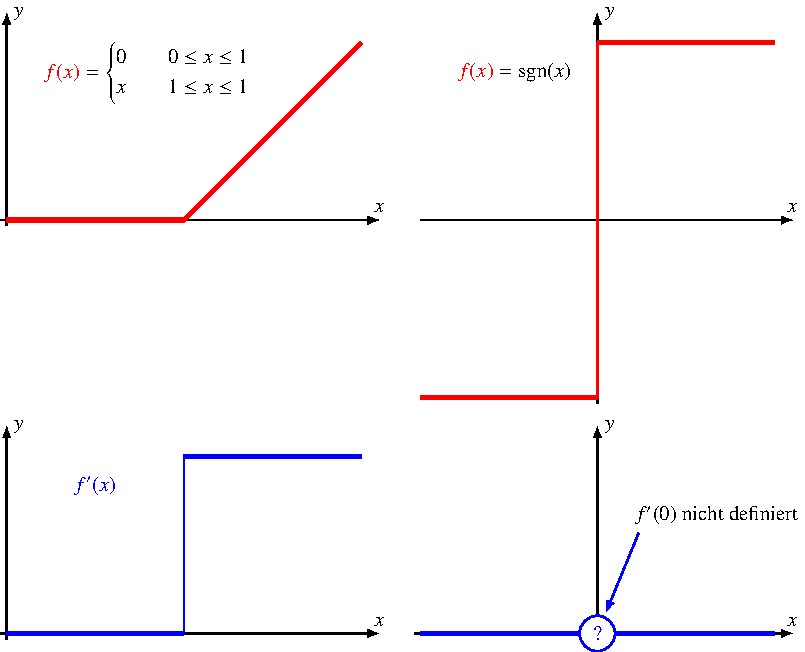
\includegraphics{chapters/010-skalarprodukt/images/schwach.pdf}
\caption{Schwache Ableitung einer nicht differenzierbaren Funktion.
Links die schwache Ableitung der Funktion von
Beispiel~\ref{buch:skalarprodukt:sobolevraum:bsp:schwachexistiert}.
Für die Signum-Funktion von
Beispiel~\ref{buch:skalarprodukt:sobolevraum:bsp:schwachexistiertnicht}
existiert die schwache Ableitung nicht, sie lässt für den Punkt $0$
nicht definieren.
\label{buch:skalarprodukt:sobolevraum:fig:schwach}}
\end{figure}
%
Die in Abbildung~\ref{buch:skalarprodukt:sobolevraum:fig:schwach} links
dargestellte Funktion
\[
f\colon (0,1) \to \mathbb{R}
:
x \mapsto
\begin{cases}
x&\qquad\text{für $0<x<1$}\\
1&\qquad\text{für $1\le x<2$}
\end{cases}
\]
ist stetig und integrierbar, aber sie ist an der Stelle $x=1$ nicht
differenzierbar.
Wir suchen die schwache Ableitung $v$ von $f$.

In einer Umgebung eines Punktes $x>1$ können wir Testfunktionen $\varphi$
so wählen, dass ihr Träger vollständig im Inneren des Intervals $(1,2)$
enthalten ist.
Mit diesen Testfunktionen können wir so rechnen, wie wenn $f$ die konstante
Funktion $1$ ist.
Das bedeutet für das Skalarprodukt
\[
\langle f,\varphi'\rangle
=
\int_1^2 \varphi'(x)\,dx
=
[\varphi(x)]_0^1 = 0.
\]
Das Skalarprodukt mit jeder beliebigen Testfunktion ist $0$, wir
müssen also $v(x)=0$ wählen.

Für $x$ im Teilinterval $(0,1)$ können wir die Testfunktionen so wählen,
dass der Träger vollständig im Inneren  von $(0,1)$ enthalten ist und
somit $f$ als die beliebig oft stetig differenzierbare Funktion $x$
behandelt werden darf.
Für das Skalarprodukt folgt dann
\[
-\langle f,\varphi'\rangle
=
-\int_0^1 f(x)\,\varphi'(x)\,dx
=
-\int_0^1 x\varphi'(x)\,dx
=
-[x\varphi(x)]_0^1 +\int_0^1 \varphi(x)\,dx
=
\langle 1,\varphi(x)\rangle,
\]
in diesem Teil des Intervals muss die schwache Ableitung den Wert $1$ 
haben.

Wir haben somit gefunden, dass die schwache Ableitung von $f$ die
Funktion
\[
v(x) = \begin{cases}
1&\qquad\text{für $0\le x<1$}
\\
0&\qquad\text{für $1< x<2$}
\end{cases}
\]
ist.
Wir kontrollieren dies, indem wir das Skalarprodukt für beliebige 
Testfunktionen $\varphi$ nachrechnen:
\begin{align*}
\langle v,\varphi\rangle
&=
\int_0^2 v(x)\,\varphi(x)\,dx
=
\int_0^1 1\,\varphi(x)\,dx
+
\int_1^2 0\,\varphi(x)\,dx.
\intertext{Jedes dieser Integrale kann man partiell integrieren:}
&=
[x\varphi(x)]_0^1 - \int_0^1 x\varphi'(x)\,dx
+
[1\varphi(x)]_1^2 - \int_1^2 1\varphi'(x)\,dx
\\
&=
\varphi(1) + \varphi(2) - \varphi(1) - \int_0^2 f(x)\,\varphi'(x)\,dx.
\intertext{Da $2$ ein Randpunkt ist, ist $\varphi(2)=0$, so dass sich}
&=-\langle f,\varphi'\rangle.
\end{align*}
ergibt.
Die Funktion $v$ ist also die schwache Ableitung von $f$.
\end{beispiel}

Eine Funktion in $W^{1,2}(\Omega)$ hat eine schwache Ableitung,
wie das Beispiel gezeigt hat, muss die Ableitung keine stetige
Funktion sein.
Ausserdem ist jede andere Funktion, die sich von der schwachen
Ableitung auf einer Menge vom Mass 0 unterscheidet, genauso eine
schwache Ableitung.
Trotzdem kann eine Funktion mit einer schwachen Ableitung nicht
beliebig ``wild'' sein, wie das folgende Beispiel zeigt.

\begin{beispiel}
\label{buch:skalarprodukt:sobolevraum:bsp:schwachexistiertnicht}
Die Signum-Funktion
\[
f\colon (-1,1) = \operatorname{sgn}(x) =
\begin{cases}
         - 1&\qquad\text{für $-1<x<0$}\\
\phantom{-}0&\qquad\text{für $x=0$}\\
\phantom{-}1&\qquad\text{für $0<x<1$}
\end{cases}
\]
ist nicht stetig (Abbildung~\ref{buch:skalarprodukt:sobolevraum:fig:schwach}).
$f$ ist fast überall konstant, in beiden Teilintervallen $(-1,0)$ und
$(0,1)$ ist die einzige mögliche schwache Ableitung von $f$ die
Nullfunktion.
Trotzdem kann $0$ nicht die schwache Ableitung von $f$ sein.
Wir wählen eine Testfunktion $\varphi$, die im Punkt $x=0$ von
Null verschieden ist.
Wäre $v$ eine schwache Ableitung von $f$, dann müsste
\begin{align*}
\langle v,\varphi\rangle
&=
-\langle f,\varphi'\rangle
=
-\int_{-1}^1 f(x) \varphi'(x)\,dx
\\
&=
-\int_{-1}^0 (-1)\cdot \varphi'(x)\,dx
-\int_{0}^1 1\cdot \varphi'(x)\,dx
=
\int_{-1}^0 \varphi'(x)\,dx
-
\int_{0}^1 \varphi'(x)\,dx
\\
&=
[\varphi(x)]_{-1}^0
-
[\varphi(x)]_{0}^1
=
\varphi(0)-\varphi(-1)
-
\varphi(1)+\varphi(0)
\\
&=
2\varphi(0)
\ne 0.
\end{align*}
Andererseits ist die Nullfunktion der einzige Kandidat für die
schwache Ableitun, für die das Skalarprodukt $\langle v,\varphi\rangle=0$
ist.
Dieser Widerspruch zeigt, dass die Funktion $f$ kein schwache
Ableitung hat.
\end{beispiel}

Die schwache Ableitung ermöglicht also mit gewissen Funktionen zu arbeiten,
die keine Ableitung im traditionellen Sinne haben.
Dank der Definition mit Hilfe eines Skalarproduktes in einem 
Hilbert-Raum darf man sich die Funktionen als Grenzwerte von
Cauchy-Folgen vorstellen.

%
% Physikalische Rechtfertigung
%
\subsection{Physikalische Rechtfertigung der schwachen Ableitung}
Die schwache Ableitung ersetzt die mit Hilfe eines Differenzenquotienten
definierte Änderungsrate durch eine Änderungsrate, die durch Vergleich
mit einer in der Umgebung eines Punktes konzentrierten Testfunktion
ermittelt wird.
Auf den ersten Blick mag das als Konzession an die Präzision der Ideen
der Analysis erscheinen, die Newton erfunden hat, um die Physik auf eine
neue Grundlage zu stellen.
Dabei wird aber vergessen, dass der Differenialquotient eine physikalisch
nicht erreichbare Idealisierung darstellt.
Keine Messung kann in einem Punkt im geometrischen Sinn erfolgen.
Die Bestimmung einer Position eines Massepunktes zum Beispiel erfolgt
durch Beobachtung des Lichtes, das vom Massepunkt reflektiert wird.
Doch der Massepunkt ist kein Punkt im geometrischen Sinn, er ist ausgedehnt
über ein endliches Gebiet.
Auch ist die Messung nicht instantan, es wird Licht gemessen, welches
über ein Zeitintervall vom Massepunkt reflektiert wird.
Das Messresultat entsteht also notwendigerweise als Mittelwert der
Beobachtung einer sehr grossen Zahl von Photonen, die von verschiedenen
Stellen reflektiert wurden.
Ein solcher Mittelwert ist genau das, was ein Skalarprodukt
$\langle f,\varphi\rangle$ mit einer Testfunktion ermittelt.

Die Feldgleichungen der Elektrodynamik wurden von Maxwell ausgehend
von Faradays Ideen als partielle Differentialgleichungen formuliert.
Sie verknüpfen die Werte des elektrischen Feldes $\vec{E}$ und des
magnetischen Feldes $\vec{B}$ mit der Ladungsdichte $\varrho$
und der Stromdichte $\vec{\jmath}$, die die Felder erzeugen.
Doch sowohl die Ladungsdichte wie auch die Stromdichte sind Idealisierungen.
Ladungen und Ströme sind nicht stetig über den Raum verteilt, sondern 
in Elektronen oder Atomkernen konzentriert.
Die Ladungsdichte entsteht daraus durch Messung der Ladung in einem kleine
Raumgebiet und Mittelung, was man wieder als Skalarprodukt mit einer
Testfunktion beschreiben kann.

Das elektrische Feld wird gemessen, indem die Kraft auf eine Testladung
im Feld ermittelt wird.
Ausser den prinzipiellen Einschränkungen an die Genauigkeit der
Positionsmessung wissen wir auch aus der Quantenmechanik, dass so etwas
wie die exakte Position eines Teilchens nicht gibt, wir können nur eine
Wahrscheinlichkeitsverteilung dafür bekommen.
Die Kraft äussert sich in einer Geschwindigkeitsänderung, die aber erst
messbar wird, wenn man die Beschleunigung eine gewisse Zeit lang aufrecht
erhält.
Das Messresultat ist also wieder ein Mittelwert über viele Positionen
und Zeitpunkte, oder anders ausgedrückt ein Skalarprodukt mit einer
Testfunktion.

Weitere Beispiele kann man auch in der Fluiddynamik finden.
Die Navier-Stokes-Gleichungen beschreiben die Strömung eines Mediums
unter der Annahme, dass es durch die Dichte $\varrho$ und die
Geschwindigkeit exakt beschreiben lässt.
Das Medium setzt sich aber aus einzelnen Atomen zusammen, die Dichte
ist also bereits ein Mittelwertbildung.
Bei der Geschwindigkeit wird das Problem noch deutlicher.
Auch die Strömungsgeschwindigkeit eines Gases ist der Mittelwert der
Strömungsgeschwindigkeit der Teilchen. 
Die Geschwindigkeit einzelner Teilchen ist dabei meistens sehr viel
grösser, nämlich im Bereich der Schallgeschwindigkeit, und äussert sich
in der Temperatur des Gases, also der mittleren kinetischen Energie.
Es ist nicht sinnvoll, von der Temperatur eines einzelnen Atoms zu
sprechen.

Alle diese Beispiele zeigen, dass die Ableitung als Änderungsrate, die
mit einem Differenzenquotienten bestimmt werden kann, eine Idealisierung
ist.
Wir können dies sogar etwas formeller zeigen.
Sei $x(t)$ die Koordinate eines Massepunktes zur Zeit $t$.
Die Messung kann nicht instantan erfolgen, im besten Fall ist die
gemessene Position ein Integral der Form
\[
\hat{x}(t)
=
\int_{-\infty}^\infty x(\tau) \varphi(\tau - t)\,d\tau.
\]
Darin ist $\varphi$ eine Testfunktion mit Träger in der Nähe von $0$.
Schreiben wir $T_t\varphi(\tau) = \varphi(\tau -t)$, dann können wir
das Messresultat auch als Skalarprodukt
$\hat{x}(t)=\langle x,T_t\varphi\rangle$
schreiben.
Die Messung mit der gleichen Aparatur einen Moment $\Delta t$ später ergibt
\[
\hat{x}(t+\Delta t)
=
\int_{-\infty}^\infty x(\tau) \varphi(\tau-t-\Delta t)\,dt
=
\langle x, T_{t+\Delta t}\varphi\rangle.
\]
Die Geschwindigkeit als Differenzenquotient ist
\begin{equation}
\frac{
\hat{x}(t+\Delta t)-\hat{x}(t)
}{\Delta t}
=
\frac{
\langle f,T_{t+\Delta t}\varphi\rangle
-
\langle f,T_{t}\varphi\rangle
}{
\Delta t
}
=
\left\langle
f,\frac{T_{t+\Delta t}\varphi - \varphi}{\Delta t}
\right\rangle
\label{buch:skalarprodukt:sobolevlraum:eqn:geschwindigkeit}
\end{equation}
Die Funktion $(T_{t+\Delta t}\varphi-T_t\varphi)/\Delta t$ ist eine 
beliebig oft stetig differenzierbare Funktion, die im Grenzwert
$\Delta t\to 0$ gegen
\[
\frac{
\varphi(\tau - t - \Delta t)
-
\varphi(\tau - t)
}{
\Delta t
}
=
-
\frac{
\varphi(\tau - t + \delta) - \varphi(\tau - t)
}{
\delta
}
\to 
-
\varphi'(\tau - t)
\quad
\text{für $\delta = - \Delta \to 0$}
\]
konvergiert.
Der Differenzenquotient
\eqref{buch:skalarprodukt:sobolevlraum:eqn:geschwindigkeit}
konvergiert daher gegen
\[
\lim_{\Delta t\to 0}
\frac{
\hat{x}(t+\Delta t)-\hat{x}(t)
}{\Delta t}
=
\left\langle
x,
\lim_{\Delta t\to 0}
\frac{T_{t+\Delta t}\varphi-T_t\varphi}{\Delta t}
\right\rangle
=
\langle f,-\varphi'\rangle
=
-
\langle f, \varphi'\rangle.
\]
Dieses einfache Modell einer ``unscharfen'' Messung führt also automatisch
auf das Konzept der schwachen Ableitung.








%\uebungsabschnitt
%\aufgabetoplevel{chapters/010-potenzen/uebungsaufgaben}
%\begin{uebungsaufgaben}
%\uebungsaufgabe{101}
%\uebungsaufgabe{102}
%\uebungsaufgabe{103}
%\uebungsaufgabe{104}
%\end{uebungsaufgaben}
%\endgroup


%
% chapter.tex -- Skalarprodukt
%
% (c) 2021 Prof Dr Andreas Müller, Hochschule Rapperswil
%
% !TeX spellcheck = de_CH
\chapter{Skalarprodukte
\label{buch:chapter:skalarprodukte}}
\kopflinks{Skalarprodukte}

%
% 1-definition.tex
%
% (c) 2023 Prof Dr Andreas Müller, OST Ostschweizer Fachhochschule
%
\section{Definition
\label{buch:opertoren:section:definition}}
\kopfrechts{Definition}


%
% 2-cauchyschwarz.tex
%
% (c) 2022 Prof Dr Andreas Müller, OST Ostschweizer Fachhochschule
%
\section{Ungleichungen
\label{buch:skalarprodukte:section:cauchyschwarz}}
\kopfrechts{Cauchy-Schwarz-Ungleichung}
In der Vektorgeometrie wird gelehrt, dass die Länge eines Vektors $u$
durch die Norm $\|u\|$ wiedergegeben wird und dass die geometrische
Intuition dazu passt.
Dazu gehört vor allem, dass die Dreiecksungleichung erfüllt ist,
dass also für drei Punkt $A$, $B$ und $C$
\begin{equation}
\overline{AB} \le \overline{AC} + \overline{BC}
\label{skalarprodukt:ungleichungen:eqn:dreieck}
\end{equation}
gilt.
In Vektorform bedeutet dies, dass
\[
\| b-a\|
\le
\| c-a\| + \|b-c\|.
\]
Schreibt man $u=c-a$ und $v=b-c$, dann ist $u+v=b-a$ und somit
\begin{equation}
\| u+v\| \le \|u\| + \|v\|.
\label{skalarprodukt:cauchyschwarz:eqn:dreieck0}
\end{equation}
Dies ist die Dreiecksungleichung in
Vektorform~\eqref{skalarprodukt:cauchyschwarz:eqn:dreieck0}.
Ziel dieses Abschnitts ist zu zeigen, dass jedes reelle oder
komplexe Skalarprodukt diese und weitere Eigenschaften automatisch
mitbringt.

%
% Cauchy-Schwarz-Ungleichung
%
\subsection{Cauchy-Schwarz-Ungleichung}
Sei also $\langle\;\,,\;\rangle$ ein reelles oder komplexes Skalarprodukt
auf dem Vektorraum $V$,
insbesondere ist $\langle v,v\rangle\ge 0$ für beliebige Vektoren $v\in V$.
Für zwei Vektoren $x,y\in V$ und $t\in \mathbb{R}$  gilt daher
\begin{align}
0
&\le
\| x+ty\|^2
=
\langle x+ty,x+ty\rangle
=
\langle x,x\rangle
+
t\langle x,y\rangle
+
t\langle y,x\rangle
+
t^2
\langle y,y\rangle.
\label{skalarprodukt:cauchyschwarz:eqn:quadrat}
\end{align}
Für ein reelles Skalarprodukt ist $\langle x,y\rangle=\langle y,x\rangle$
und damit
\begin{align}
0
&\le
\|x\|^2 + 2t\langle x,y\rangle + t^2 \|y\|^2.
\label{buch:skalarprodukt:cauchyschwarz:eqn:cspoly}
\end{align}
Dies ist ein quadratisches Polynom in der Variablen $t$, dessen Minimum
nicht negativ sein darf.

%
% Minimum eines quadratischen Polynoms
%
\subsubsection{Minimum eines quadratischen Polyoms}
Ein beliebiges quadratisches Polynom
\[
p(t)=at^2+bt+c
\]
kann durch
quadratisches Ergänzen in die Form
\[
p(t)
=
a\biggl(t+\frac{b}{2a}\biggr)^2 -\frac{b^2}{4a}+c
\]
gebracht werden.
Daraus kann man ablesen, dass das Minimum an der Stelle
\[
t_0
=
-\frac{b}{2a}
\]
angenommen wird und den Wert 
\begin{equation}
p(t_0)
=
c-\frac{b^2}{4a}
\end{equation}
hat.
Die gleiche Lösung kann natürlich auch durch Bestimmung des Minimums
von $p(t)$ mit Hilfe der Bedingung $p'(t_0)=0$ gefunden werden.

%
% Cauchy-Schwarz-Ungleichung für einen reellen Vektorraum
%
\subsubsection{Cauchy-Schwarz-Ungleichung für einen reellen Vektorraum}
Für~\eqref{buch:skalarprodukt:cauchyschwarz:eqn:cspoly}
ist
\[
a=\|y\|^2,\quad
b=2\langle x,y\rangle
\quad\text{und}\quad
c=\|x\|^2.
\]
Daher folgt aus~\eqref{buch:skalarprodukt:cauchyschwarz:eqn:cspoly}
\[
0
\le
\|x\|^2 - \frac{\langle x,y\rangle^2}{\|y\|^2}
\qquad\Rightarrow\qquad
\langle x,y\rangle^2 \le \|x\|^2\, \|y\|^2
\qquad\Rightarrow\qquad
|\langle x,y\rangle| \le \|x\|\, \|y\|.
\]
Dies ist die Cauchy-Schwarz-Ungleichung für das Skalarprodukt
$\langle \;\,,\;\rangle$.

\begin{satz}[Cauchy-Schwarz]
\label{buch:skalarprodukt:cauchy-schwarz:satz:reell}
Ein reelles Skalarprodukt $\langle\;\,,\;\rangle$ auf dem reellen Vektorraum
$V$ erfüllt die Cauchy-Schwarz-Ungleichung
\[
|\langle x, y\rangle| \le \|x\|\,\|y\|
\]
für $x,y\in V$.
\end{satz}

%
% Cauchy-Schwarz-Ungleichung für einen komplexen Vektorraum
%
\subsubsection{Cauchy-Schwarz-Ungleichung für einen komplexen Vektorraum}
Für ein komplexes Skalarprodukt ist das Produkt $\langle x,y\rangle$
nicht mehr unbedingt reell und kann damit nicht mehr direkt mit den
Normen $\|x\|^2u$ und $\|y\|^2$ vergleichen.
Wir ersetzen daher $t$ durch
$t\langle y,x\rangle=t\overline{\langle x,y\rangle}$
und erhalten 
\begin{align*}
0
\le
\|x+t\langle y,x\rangle y\|^2
&=
\langle x,x\rangle
+t\langle y,x\rangle \langle x,y\rangle
+t\overline{\langle y,x\rangle}\langle y,x\rangle
+t^2\langle y,y\rangle
\\
&=
\|x\|^2
+
t
2|\langle x,y\rangle|^2
+
t^2 |\langle x,y\rangle|^2
\|y\|^2.
\end{align*}
Dies ist wieder ein quadratisches Polynom, diesmal mit den Koeffizienten
\[
a= |\langle x,y\rangle|^2 \|y\|^2,
\quad
b= 2|\langle x,y\rangle|^2
\quad\text{und}\quad
c= \|x\|^2.
\]
Das Minimum dieses Polynoms ist nach
\[
0
\le
c-\frac{b^2}{4a}
=
\|x\|^2 - \frac{|\langle x,y\rangle|^4}{|\langle x,y\rangle|^2\,\|y\|^2}
=
\|x\|^2 - \frac{|\langle x,y\rangle|^2}{\|y\|^2}
\quad\Rightarrow\quad
|\langle x,y\rangle|^2 \le \|x\|^2\,\|y\|^2
\quad\Rightarrow\quad
|\langle x,y\rangle \le \|x\|\,\|y\|.
\]
Dies ist die Cauchy-Schwarz-Ungleichung für einen komplexen Vektorraum.

\begin{satz}[Cauchy-Satz]
\label{buch:skalarprodukt:cauchy-schwarz:satz:komplex}
Ein komplexes Skalarprodukt $\langle\;\,,\;\rangle$ auf dem komplexen Vektorraum
$V$ erfüllt die Cauchy-Schwarz-Ungleichung
\[
|\langle x, y\rangle| \le \|x\|\,\|y\|
\]
für $x,y\in V$.
\end{satz}

Man beachte, dass die
Sätze~\ref{buch:skalarprodukt:cauchy-schwarz:satz:reell}
und
\ref{buch:skalarprodukt:cauchy-schwarz:satz:komplex}
nur die Axiome eines Skalarproduktes verwenden.
Sie gelten also
ganz unabhängig von der konkreten Definition des Skalarproduktes,
solange die Eigenschaften eines Skalarproduktes gegeben sind.

\begin{beispiel}
Die sesquilineare Funktion
\[
\langle x,y\rangle
=
\sum_{i=1}^n\overline{x}_i y_i
\]
für Vektoren $x,y\in\mathbb{C}^n$ ist positiv definit, denn
\[
\langle x,x\rangle
=
\sum_{i=1}^n \overline{x}_i x_i = \sum_{i=1}^n |x_i|^2 > 0
\]
für $x\ne 0$.
Nach Satz~\ref{buch:skalarprodukt:cauchy-schwarz:satz:komplex}
gilt daher
\[
\biggl|
\sum_{i=1}^n \overline{x}_i y_i
\biggr|
\le
\sqrt{\sum_{i=1}^n |x_i|^2} \sqrt{\sum_{i=1}^n |y_i|^2}
\quad\text{oder auch}\quad
\biggl|
\sum_{i=1}^n x_i y_i
\biggr|
\le
\sqrt{\sum_{i=1}^n |x_i|^2} \sqrt{\sum_{i=1}^n |y_i|^2}
\]
für beliebige Vektoren $x,y\in\mathbb{C}^n$.
\end{beispiel}

\begin{beispiel}
Die sesquilineare Funktion
\[
\langle f,g\rangle
=
\int_a^b \overline{f(x)} g(x)\,dx
\]
für komplexwertige, stetige Funktion auf dem Intervall $[a,b]$
ist positiv definit, denn
\[
\langle f,f\rangle
=
\int_a^b \overline{f(x)} f(x)\,dx
=
\int_a^b |f(x)|^2\,dx
\ge 0
\]
für $f\ne 0$.
Nach Satz~\ref{buch:skalarprodukt:cauchy-schwarz:satz:komplex}
gilt daher
\begin{align*}
\biggl|\int_a^b \overline{f(x)}g(x)\,dx\biggr|
&\le
\sqrt{\int_a^b |f(x)|^2\,dx}
\sqrt{\int_a^b |g(x)|^2\,dx}
\intertext{oder auch}
\biggl|\int_a^b f(x) g(x)\,dx\biggr|
&\le
\sqrt{\int_a^b |f(x)|^2\,dx}
\sqrt{\int_a^b |g(x)|^2\,dx}
\end{align*}
für beliebige komplexwertige stetige Funktionen $f,g$ auf dem
Intervall $[a,b]$.
\end{beispiel}

%
% Dreiecksungleichung
%
\subsection{Dreiecksungleichung}
Die Intuition einer Längenmessung basiert auf der
Dreiecksungleichung~\eqref{skalarprodukt:ungleichungen:eqn:dreieck}.
Sie ist gleichbedeutend mit der
Vektorform~\eqref{skalarprodukt:cauchyschwarz:eqn:dreieck0}
der Ungleichung.

Die Cauchy-Schwarz-Ungleichung ermöglicht nun, diese Ungleichung
nachzurechnen.
Die Norm von $\|x+y\|^2$ ist
\[
\|x+y\|^2
=
\langle x+y,x+y\rangle
=
\langle x,x\rangle
+
\langle x,y\rangle
+
\langle y,x\rangle
+
\langle y,y\rangle
=
\|x\|^2 + 2\operatorname{Re}\langle x,y\rangle + \|y\|^2.
\]
Den mittleren Term kann man mit der Cauchy-Schwarz-Ungleichung
umformen:
\begin{align*}
\|x\|^2 + 2\operatorname{Re}\langle x,y\rangle + \|y\|^2.
&\le
\|x\|^2 + 2|\operatorname{Re}\langle x,y\rangle| + \|y\|^2.
\\
&\le
\|x\|^2 + 2|\langle x,y\rangle| + \|y\|^2.
\\
&\le
\|x\|^2 + 2\|x\|\,\|y\| + \|y\|^2
=
(\|x\| + \|y\|)^2.
\end{align*}
Durch Ziehen der Wurzel folgt
\[
\|x+y\| \le \|x\| + \|y\|.
\]
Damit ist der folgende Satz bewiesen.

\begin{satz}[Dreiecksungleichung]
Für die Norm zu einem beliebigen Skalarprodukt auf dem reellen
oder komplexen Vektorraum $V$ gilt die Dreiecksungleichung
\[
\|x+y\| \le \|x\| + \|y\|
\]
für $x,y\in V$.
\end{satz}

%
% Normen
%
\subsection{Normen
\label{skalarprodukt:cauchyschwarz:subsection:norm}}
Das Skalarprodukt ist nicht die einzige Möglichkeit, eine Norm auf
einem Vektorraum zu definieren.
Zum Beispiel kann man auf $\mathbb{C}^n$ die sogenannte $l^1$-Norm
definieren.

\begin{definition}
Die Funktion
\[
\|x\|_1
=
\sum_{i=1}^n |x_i|
\]
für $x\in\mathbb{C}^n$ heisst die {\em $l^1$-Norm} auf $\mathbb{C}^n$.
\end{definition}

Die Funktion $\|\cdot\|_1$ ist eine Norm im Sinne der folgenden Definition.

\begin{definition}
Eine Funktion $\|\cdot\| \colon V\to\mathbb{R}$ auf einem reellen
oder komplexen Vektorraum $V$ heisst eine {\em Norm}, wenn Sie die
folgenden Bedingungen erfüllt
\begin{enumerate}
\item
$\|\lambda x\| = |\lambda|\, \|x\|$ für $x\in V$ und $\lambda\in \Bbbk$
\item
Für alle Vektoren $x\in V$ mit $x\ne 0$ gilt $\|x\|>0$.
\item
Dreiecksungleichung: $\|x+y\| \le \|x\| + \|y\|$ für alle $x,y\in V$
\end{enumerate}
\end{definition}

Es ist klar, dass die $l^1$-Norm die Bedingungen~1 und 2 erfüllt.
Aber auch die Bedingung~3 kann man leicht  nachprüfen:
\[
\|x+y\|_1
=
\sum_{i=1}^n |(x+y)_i|
=
\sum_{i=1}^n |x_i+y_i|
\le
\sum_{i=1}^n(|x_i|+|y_i|)
=
\sum_{i=1}^n|x_i|
+
\sum_{i=1}^n|y_i|
=
\|x\|_1 + \|y\|_1,
\]
wozu wir nur die Dreiecksungleichung $|a+b|\le |a| + |b|$ für reelle 
oder komplexe Zahlen $a,b$ benötigen.

\begin{beispiel}
Die Funktion
\[
\|x\|_\infty = \sup_{1\le i\le n} |x_i|
\]
ist eine Norm auf $\mathbb{C}^n$.
\end{beispiel}

Auch in diesem Fall sind die Bedingungen~1 und 2 ganz offensichtlich erfüllt.
Für die Dreiecksungleichung rechnen
\begin{align*}
\|x+y\|_\infty
&=
\sup_{1\le i\le n} |x_i+y_i|
\le
\sup_{1\le i\le n} (|x_i|+|y_i|)
\le
\sup_{1\le i\le n} |x_i|+\sup_{1\le i\le n}|y_i|
=
\|x\|_\infty + \|y\|_\infty.
\end{align*}
Somit ist $\|\cdot\|_\infty$ eine Norm auf $\mathbb{C}^n$.

%
% Polaridentität
%
\subsection{Polaridentität}
Die durch das Skalarprodukt definierte Norm
\( \|x\|^2=\langle x,x\rangle \)
ist nach Abschnitt~\ref{skalarprodukt:cauchyschwarz:subsection:norm}
ein Spezialfall einer Norm.
Ist es möglich, für eine Norm, die von einem Skalarprodukt herkommt,
das Skalarprodukt wieder zu rekonstruieren?

%
% Reelles Skalarprodukt aus der Norm
%
\subsubsection{Reelles Skalarprodukt aus der Norm}
Die Antwort gibt der folgende Satz.

\begin{satz}[Polaridentität]
\label{skalarprodukt:cauchyschwarz:satz:polarformel}
Ist $\|\cdot\|$ die Norm zu einem Skalarprodukt auf dem reellen Vektorraum
$V$, dann kann das Skalarprodukt zweier Vektoren $x,y\in V$ mittels
der sogenannten {\em Polaridentität}
\index{Polaridentität}%
\begin{equation}
\langle x, y\rangle
=
\frac12\bigl(
\|x+y\|^2 - \|x\|^2 - \|y\|^2 
\bigr)
\label{skalarprodukt:cauchyschwarz:eqn:polar}
\end{equation}
berechnet werden.
\end{satz}

\begin{proof}[Beweis]
Die Gleichung
\begin{align*}
\|x+y\|^2
&=
\langle x+y,x+y\rangle
=
\|x\|^2 + 2\langle x,y\rangle + \|y\|^2 
\end{align*}
kann nach $\langle x,y\rangle$ aufgelöst werden und ergibt
die behauptete Formel~\eqref{skalarprodukt:cauchyschwarz:eqn:polar}.
\end{proof}

% 
% Parallelogrammgleichung
%
\subsubsection{Parallelogrammgleichung}
\begin{figure}
\centering
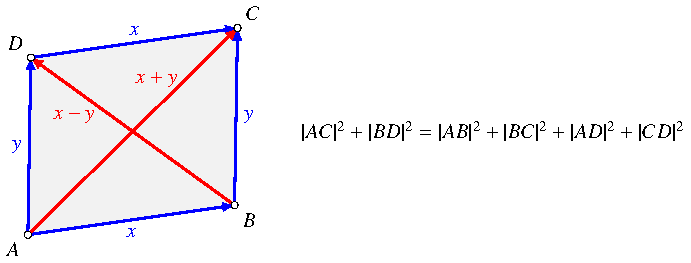
\includegraphics{chapters/010-skalarprodukt/images/parallelogramm.pdf}
\caption{Parallelogrammregel für eine Norm, die aus einem Skalarprodukt
entsteht.
\label{skalarprodukt:cauchyschwarz:fig:parallelogramm}}
\end{figure}
Die Polaridentitäten können auch noch in einer anderen Form geschrieben
werden.
Dazu berechnet man zusätzlich die Norm von $x-y$:
\begin{align*}
\|x+y\|^2
&=
\|x\|^2 + \|y\|^2 + 2\langle x, y\rangle
\\
\|x-y\|^2
&=
\|x\|^2 + \|y\|^2 - 2\langle x, y\rangle
\\
\|x+y\|^2 +\|x-y\|^2
&=
2\|x\|^2 + 2\|y\|^2
\end{align*}

\begin{satz}
\label{skalarprodukt:cauchyschwarz:satz:parallelgramm}
Für eine Norm, die von einem reellen Skalarprodukt herkommt, gilt die
Parallelogrammformel
\begin{equation}
\|x+y\|^2 +\|x-y\|^2
=
2\|x\|^2 + 2\|y\|^2.
\label{skalarprodukt:cauchyschwarz:eqn:parallelgramm}
\end{equation}
(Abbildung~\ref{skalarprodukt:cauchyschwarz:fig:parallelogramm})
\end{satz}

Das Skalarprodukt kann man damit auf verschiedene Weise aus der
Norm gewinnen:
\begin{equation}
\begin{aligned}
\langle x, y\rangle
&=
{\textstyle\frac12}\bigl( \|x\|^2 + \|y\|^2 - \|x+y\|^2 \bigr)
\\
&=
{\textstyle\frac12}\bigl(
\|x+y\|^2
-
\|x\|^2 
-
\|y\|^2
\bigr)
\\
&=
{\textstyle\frac14}\bigl(
\|x+y\|^2 - \|x-y\|^2
\bigr).
\end{aligned}
\label{skalarprodukt:cauchyschwarz:eqn:realteil}
\end{equation}
Nur die letzte Formel ist noch nicht gut begründet.
Man kann aber sofort nachrechnen, dass 
\begin{align*}
\|x+y\|^2&=\|x\|^2+2\langle x,y\rangle+\|y\|^2\\
\|x-y\|^2&=\|x\|^2-2\langle x,y\rangle+\|y\|^2
\intertext{die Differenz}
\|x+y\|^2 - \|x-y\|^2 &= 4\langle x,y\rangle
\qquad
\Rightarrow
\qquad
\langle x,y\rangle
=
\frac14\bigl(\|x+y\|^2 - \|x-y\|^2\bigr)
\end{align*}
haben.

%
% Komplexes Parallelogramm aus der Norm
%
\subsubsection{Komplexe Skalarprodukt}
Das Resultat von Satz~\ref{skalarprodukt:cauchyschwarz:satz:polarformel}
gilt in abgeänderter Form auch für komplexe Skalarprodukte.
Da das Skalarprodukt auch einen nichtverschwindenen Imaginärteil haben
kann, wird eine zusätzliche Gleichung zur Berechnung des Imaginärteils
nötig.
Eine solche kann gewonnen werden, indem zusätzlich die Normen
$\|x+iy\|^2$ und $\|x-iy\|^2$ berechnet werden.
Dazu ist zu beachten, dass
\[
\langle x,y\rangle
-
\langle y,x\rangle
=
\langle x,y\rangle
-
\overline{
\langle x,y\rangle
}
=
2i\operatorname{Im}\langle x,y\rangle
\]
Damit erhält man
\begin{align*}
\|x+iy\|^2 &= \|x\|^2 + i\langle x,y\rangle - i\langle y,x\rangle + \|y\|^2 
           = \|x\|^2 + 2\operatorname{Im}\langle x,y\rangle + \|y\|^2 \\
\|x-iy\|^2 &= \|x\|^2 - i\langle x,y\rangle + i\langle y,x\rangle + \|y\|^2 
           = \|x\|^2 - 2\operatorname{Im}\langle x,y\rangle + \|y\|^2.
\end{align*}
Damit kann man nach dem Imaginärteil des Skalarproduktes auflösen und
die Formeln
finden, die den Formeln
\eqref{skalarprodukt:cauchyschwarz:eqn:realteil}
für das reelle Skalarprodukt entsprechen.
\eqref{skalarprodukt:cauchyschwarz:eqn:realteil}
Formeln bleiben gültig als Formeln für den Realteil des Skalarproduktes.
Damit haben wir den folgenden Satz gefunden.

\begin{satz}[Polaridentitäten für ein komplexes Skalarprodukt]
Ist $\|\cdot\|$ die Norm, die aus dem komplexen Skalarprodukt
$\langle\;\,,\;\rangle$ auf einem Vektorraum $V$ gewonnen wurde,
dann können Real- und Imaginärteil mit den Formeln
\begin{align*}
\operatorname{Re}\langle x,y\rangle
&=
{\textstyle\frac12}\bigl(
\|x+y\|^2 - \|x\|^2 -\|y\|^2
\bigr)
\\
&=
{\textstyle\frac12}\bigl(
\|x\|^2 +\|y\|^2 - \|x+y\|^2
\bigr)
\\
&=
{\textstyle\frac14}\bigl(
\|x+y\|^2 - \|x-y\|^2
\bigr),
\\
\operatorname{Im}\langle x,y\rangle
&=
{\textstyle\frac12}\bigl(
\|x+iy\|^2-\|x\|^2-\|y\|^2
\bigr)
\\
&=
{\textstyle\frac12}\bigl(
\|x\|^2+\|y\|^2-\|x-iy\|^2
\bigr)
\\
&=
{\textstyle\frac14}\bigl(
\|x+iy\|^2
-
\|x-iy\|^2
\bigr)
\end{align*}
für beliebige Vektoren $x,y\in V$
allein aus Werten der Norm berechnet werden.
\end{satz}


%
% 3-funktionenraeume.tex
%
% (c) 2022 Prof Dr Andreas Müller, OST Ostschweizer Fachhochschule
%
\section{Funktionenräume
\label{buch:skalarprodukt:section:funktionenraeume}}
\kopfrechts{Funktionenräume}
Ziel der harmonischen Analysis ist die effiziente Approximation einer
grossen Klasse von Funktionen.
Als approximierende Funktionen kommen stetige Funktionen, Polynome,
trigonometrische Polynome oder eine ähnlich, einfach konstruierbare
Funktionenfamilie in Frage.
Es gilt zunächst herauszufinden, was ``Approximation'' genau heissen
soll und von welchen Funktionen man überhaupt erwarten kann, dass sie
approximiert werden können.

%
% Stetige Funktionen
%
\subsection{Stetige Funktionen
\label{buch:skalarprodukt:subsection:stetige-funktionen}}
Der frühe intuitive Funktionsbegriff ging oft von der Vorstellung einer
in einem Strich gezeichneten Kurve aus, wie man sie von den Graphen
der Polynome oder der trigonometrischen Funktionen her kennt.
In moderner Sprechweise sind dies die stetigen Funktionen.

\begin{definition}
Eine Funktion $f\colon I\to\mathbb{R}$ mit $I\subset \mathbb{R}$
heisst stetig in einem Punkt $x_0\in I$, wenn für jedes $\varepsilon>0$
ein $\delta>0$ existiert derart, dass $f(x)-f(x_0)|<\delta$ sobald
$|x-x_0|<\varepsilon$.
\end{definition}

Nur die Eigenschaft, eine Abstandsmessung zu besitzen, wird vom
Definitionsbereich $I\subset \mathbb{R}$ verlangt.
Der Stetigkeitsbegriff kann daher verallgemeinert werden auf den
Begriff des metrischen Raumes.

\begin{definition}
Eine {\em Metrik} auf einer Menge $X$ ist eine Funktion
\index{Metrik}%
$d\colon X\times X\to \mathbb{R}$
mit den folgenden Eigenschaften
\begin{enumerate}
\item
Positiv definit: $d(x,y)\ge 0$ und $d(x,y)$ genau dann, wenn $x=y$.
\item
Symmetrie: \(d(x,y)=d(y,x)\)
\item
Dreiecksungleichung: \( d(x,y) \le d(x,z) + d(z,y) \).
\end{enumerate}
Ein {\em metrischer Raum} ist ein Menge $X$ mit einer Metrik.
\index{matrischer Raum}%
\end{definition}

In einem metrischen Raum ist der Begriff des Grenzwertes übertragbar.
Mit dem Begriff des Grenzwertes lässt sich auch der Begriff der
Stetigkeit verallgemeinern.

\begin{definition}
Ist $x_n\in X$ eine Folge von Punkten in einem metrischen Raum $X$,
dann heisst $x$ der Grenzwert der Folge $x_n$, wenn es für jedes
$\varepsilon>0$ ein $N>0$ gibt derhart, dass
$d(x_n,x)\le \varepsilon$ für alle $n>N$.
Eine Funktion $f\colon X\to Y$ zwischen metrischen Räumen heisst
stetig im Punkt $x\in X$, wenn für jede Folge $x_n\in X$ mit
Grenzwert $x$ auch die Folge $y_n=f(x_n)\in Y$ konvergiert und
den Grenzwert $y=f(x)$ hat.
\end{definition}

Teilmengen von $\mathbb{R}$ oder $\mathbb{R}^n$ tragen natürlich
die Struktur eines metrischen Raumes mit der Abstandsmessung in 
$\mathbb{R}^n$ als Metrik
\[
d(x,y) = \sqrt{(x_1-y_1)^2 + \ldots + (x_n-y_n)^2} = \|x-y\|.
\]
Die Eigenschaften einer Metrik wurden bereits in Abschnitt
\ref{buch:skalarprodukte:section:cauchyschwarz} nachgewiesen.

Der Begriff des Grenzwertes klärt, was mit der Approximation von $x$
durch eine Folge $x_n$ gemeint ist.
Wenn man darauf aufbauend die Konvergenz einer Folge von Funktionen
gegen eine Grenzfunktion definieren will, braucht man einen Abstansbegriff
zwischen Funktionen.
Ein erster Versuch könnte sein, als Abstand zwischen zwei Funktionen
$f$ und $g$ die Funktion
\[
d(f,g) = |f(x_0) - g(x_0)|.
\]
Die Menge der Funktionen wird dadurch jedoch nicht zu einem metrischen
Raum.
Zwar gilt sicher die Symmetrie und Dreiecksungleichung, und auch 
$d(f,g)\ge 0$ für beliebige Funktionen.
Aber wenn $d(f,g)=0$ ist, heisst das nur, dass $f$ und $g$ im Punkt
$x_0$ den gleichen Wert haben.
Ausser in trivialen Fällen wird es Funktionen geben, die zwar im Punkt
$x_0$ übereinstimmen, sich aber in mindestens einem anderen Punkt
unterscheiden.

%
% Normierte Räume
%
\subsubsection{Normierte Räume}
Die stetigen Funktionen bilden aber keine strukturlose Menge, sie
bilden einen Vektorraum: die Summe von stetigen Funktionen ist ebenfalls
stetig, multiplizieren einer stetigen Funktion mit einem Skalar führt
nicht aus der Menge der stetigen Funktionen heraus.
Die für den Grenzwertbegriff von Funktionen verwendete Abstandsmessung 
sollte der Vektorraumstruktur ebenfalls Rechnung tragen.

\begin{definition}
\label{buch:skalaprodukt:funktionenraume:def:norm}
Sei $V$ ein Vektorraum über $\mathbb{R}$, dann heisst eine Funktion
\( \|\;\cdot\;\| \colon V \to \mathbb{R}\) eine {\em Norm}, wenn gilt
\index{Norm}
\begin{enumerate}
\item
Definit: $ \|x\| = 0 \Rightarrow x=0$
\item
Homogeneität: $ \| \lambda x \| = |\lambda| \cdot \|x\|$
\item
Dreiecksungleichung: $\|x+y\| \le \|x\| + \|y\|$
\end{enumerate}
Ein {\em normierter Raum} ist ein Vektorraum $V$ mit einer Norm.
\end{definition}

%
% Vollständigkeit
%
\subsubsection{Vollständigkeit}
In den rationalen Zahlen hat nicht jede Folge einen Grenzwert.
Die Zahl $\sqrt{2}$ lässt sich beliebig genau durch rationale Zahlen
approximieren, sie ist aber nicht in $\mathbb{Q}$.
Ähnlich lässt sich die Funktion $x\mapsto \sqrt{x}$ beliebig genau 
durch Polyome approximieren, sie ist aber selbst kein Poylnome

\begin{definition}
Ein Folge $x_n\in X$ in einem metrischen Raum heisst {\em Cauchy-Folge},
wenn es für jedes $\varepsilon>0$ ein $N>0$ gibt derart, dass 
$|x_n-x_m|<\varepsilon$ wenn $n,m>N$ ist.
\end{definition}

Cauchy-Folgen sind also Folgen, die sich für genügend grossen Index
kaum mehr ändern und für die man daher Konvergenz erwarten würde.

\begin{definition}
Ein normierter Raum heisst {\em vollständig} oder ein Banach-Raum,
wenn jede Cauchy-Folge einen Grenzwert hat.
\end{definition}

Die rationalen Zahlen $\mathbb{Q}$ bilden keinen vollständigen
metrischen Raum, aber die reellen Zahlen $\mathbb{R}$ enthalten
alle Grenzwerte von Cauchy-Folgen, $\mathbb{R}$ ist eine vollständiger
metrischer Raum.
Die Menge der Polynome, betrachtet als Teilmenge der Menge der
stetigen Funktionen $[0,1]\to\mathbb{R}$ ist nicht vollständig,
da es eine Folge $f_n(x)$ von Approximationsfunktionen der Funktion
$x\mapsto \sqrt{x}$ gibt.
Als Cauchy-Folge konvergiert sie zwar gegen eine stetige Funktion,
aber die Grenzfunktion ist nicht mehr im Raum der Polynome.

Das Ziel der folgenden Kapitel ist also, zu geeignet interessanten
Funktionenfamilien ``gute'' Normen zu finden derart, dass Cauchy-Folgen
konvergieren gegen Funktionen, die immer noch ausreichend viele
nützliche Eigenschaften haben.
Im besten Fall konvergieren stetige Funktionen gegen stetige Funktionen,
es wird sich aber zeigen, dass diese Anforderung zu streng ist.

%
% Norm fpr stetige Funktionen
%
\subsection{Norm für stetige Funktionen
\label{buch:skalarprodukt:subsection:normfuerstetigefunktionen}}
Damit man von Konvergenz von Folgen stetiger Funktionen sprechen kann,
brauchen wir jetzt also eine Norm für stetige Funktionen.

\begin{definition}
Sei $X$ ein metrischer Raum und
\[
C(X)
=
C_{\mathbb{R}}(X)
=
\{
f\colon X \to\mathbb{R}\mid
\text{$f$ ist stetig}
\}
\]
der Vektorraum der stetigen Funktion auf $X$.
Die Norm von $C(X)$ ist definiert als
\[
\|f\| = \sup_{x\in X} |f(x)|.
\]
Sie heisst die {\em Supremum-Norm}.
\end{definition}

Wir prüfen nach, dass die Supremum-Norm tatsächlich eine Norm ist.
Dazu sind die definierenden Eigenschaften nachzurechnen:
\begin{enumerate}
\item Definit: 
\[
0
=
\|f\|
=
\sup_{x\in X} |f(x)|
\quad\Rightarrow\quad
f(x)=0 \;\forall x\in X
\quad\Rightarrow\quad
f\in C(X).
\]
\item Homogeneität:
\[
\|\lambda f\|
=
\sup_{x\in X} |\lambda f(x)|
=
|\lambda| \sup_{x\in X} |f(x)|
=
|\lambda| \cdot \|f\|.
\]
\item
Dreiecksungleichung:
\[
\|f+g\|
=
\sup_{x\in X}|f(x)+g(x)|
\le
\sup_{x\in X}(|f(x)|+|g(x)|)
\le
\sup_{x\in X}|f(x)|+\sup_{x\in X}|g(x)|
=
\|f\| + \|g\|.
\]
\end{enumerate}

Eine Cauchy-Folge $f_n$ von Funktionen $X\to \mathbb{R}$ hat die
Eigenschaft, dass für jedes $\varepsilon >0$ ein $N>0$ existiert,
derart dass $\|f_n-f_m\|<\varepsilon$ ist.
Da die Norm der maximale Unterschied von Funktionswerten ist,
folgt dass für eine Cauchy-Folge in $C(X)$ die Folge $f_n(x)$ eine
Cauchy-Folge in $\mathbb{R}$ ist und damit einen Grenzwert in $\mathbb{R}$
hat.
Die Funktion $f(x) = \lim_{n\to\infty}f_n(x)$ ist die Grenzfunktion.
Die Konvergenz bezüglich der Norm besagt, dass für jedes $\varepsilon>0$
es ein $N>0$ gibt derart, dass
\[
\varepsilon 
>
\|f_n-f\|
\ge 
|f_n(x)-f(x)|
\]
ist für alle $n>N$ und unabhängig von $x\in X$.
Die Konvergenz bezüglich der $\|\;\cdot\;\|$-Norm ist also die wohlbekannte
gleichmässige Konvergenz.
Es kann gezeigt werden, dass die Grenzfunktion wieder stetig ist.

\begin{satz}
Der Raum der stetigen Funktion $C(X)$ mit der Supremumg-Norm ist
ein Banach-Raum.
\end{satz}

%
% Skalarprodukt
%
\subsection{Skalarprodukt
\label{buch:skalarprodukt:subsection:skalarprodukt}}
\begin{figure}
\centering
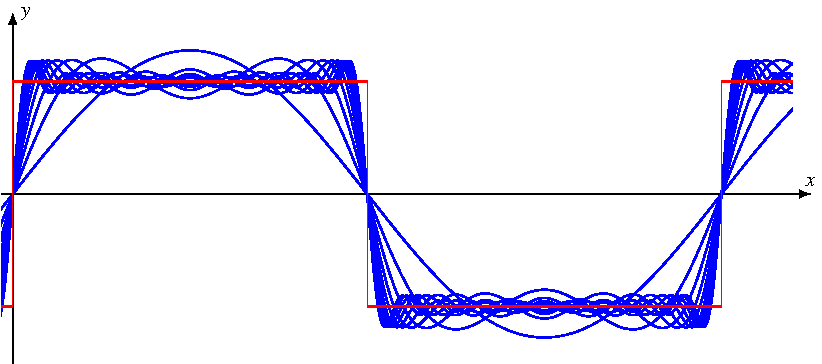
\includegraphics{chapters/010-skalarprodukt/images/fourierrechteck.pdf}
\caption{Approximation der Rechteckfunktion (rot) durch eine Folge
von Partialsummen der Fourier-Reihe.
\label{buch:skalarprodukt:fig:fourierrechteck}}
\end{figure}%
Die Supremum-Norm auf dem Raum der stetigen Funktionen hat den
Begriff der gleichmässig konvergenten Funktionenfolgen ergeben.
Cauchy-Folgen von stetigen Funktionen in der Supremum-Norm konvergieren
wieder gegen eine stetige Funktione.
Ist eine Funktion nicht stetig, lässt Sie sich im Sinne der Supremum-Norm
nicht durch stetige Funktionen approximieren.
Andererseits hat Fourier gezeigt, wie man technische wichtige Funktionen
wie die Rechteckfunktion durch trigonometrische Polynome
\begin{equation}
f_n(x)
=
\frac{4}{\pi} \sum_{k=0}^n \frac{\sin kx}{k}
=
\frac{4}{\pi} \biggl(
\sin x
+
\frac{\sin 3x}{3}
+
\frac{\sin 5x}{5}
+
\frac{\sin 7x}{7}
+
\ldots
\biggr)
\label{buch:skalarprodukt:eqn:rechteckreihe}
\end{equation}
approximieren kann.
Diese sind alle stetig und kommen der Rechteckfunktion in jedem Punkt,
in dem die Funktion stetig ist, beliebig nahe.
An den Stellen $x = n\pi$ hat die Grenzfunktion eine Sprungstelle,
die approximierenden Funktionen haben dort immer Abstand $1$
(siehe Abbildung~\ref{buch:skalarprodukt:fig:fourierrechteck}).
Die Folge ist also keine Cauchy-Folge und sie konvergiert nicht im
Sinne der Supremum-Norm.
Für solche Anwendungen muss eine besser geeignete Norm gefunden werden,
in der die Folge konvergiert.

%
% Skalarprodukt von Funktion
%
\subsubsection{Die $L^1$-Norm einer Funktion}
Die Supremum-Norm sieht nur den grössten Wert, die Konvergenz der Folge
\eqref{buch:skalarprodukt:eqn:rechteckreihe} ist aber nicht gleichmässig,
die maximale Abweichung ist immer $1$.
Gesucht ist eine Norm, die für die Folge
\eqref{buch:skalarprodukt:eqn:rechteckreihe} 
nur im Mittel eine Abweichung feststellt.
Für die Berechnung des Mittelwerts kann das Integral verwendet werden:

\begin{definition}
\label{buch:skalaprodukt:definition:l1norm}
Für eine stetige Funktion $X\to\mathbb{R}$, für die $x\mapsto |f(x)|$
integrierbar ist, heisst
\begin{equation}
\|f\|_1 = \int_X |f(x)|\,dx
\label{buch:skalarprodukt:eqn:l1norm}
\end{equation}
die {\em $L^1$-Norm} der Funktion $f$.
\end{definition}

Die $L^1$-Norm ist tatsächlich eine Norm, wir verifizieren die
definierenden Eigenschaften einer Norm.
\begin{enumerate}
\item
Definit: Sei $f$ eine stetige Funktion mit $\|f\|_1=0$
Wäre $f\ne 0$, dann gäbe es einen Punkt $x_0\in X$ mit $f(x_0) \ne 0$.
Da $f$ stetig ist, ist $f|(x)| > \frac12|f(x_0)|$ für $x$ in einer
$\delta$-Umgebung von $x_0$.
Dann folgt für die $L^1$-Norm
\begin{align*}
\|f\|_1
=
\int_X |f(x)|\,dx
\ge
\frac12 |f(x_0)| \cdot \delta 
> 0.
\end{align*}
Dies widerspricht der Annahme, dass $\|f\|_1=0$ ist, also muss $f=0$ sein.
\item
Homogeneität folgt durch direkte Rechnung
\[
\|\lambda f\|_1
=
\int_X |\lambda f(x)|\,dx
=
|\lambda|
\int_X |f(x)|\,dx
=
|\lambda| \cdot \|f\|.
\]
\item
Die Dreiecksungleichung folgt aus
\[
\|f+g\|_1
=
\int_X |f(x) + g(x)|\,dx
\le
\int_X |f(x)| + |g(x)|\,dx
=
\int_X |f(x)| + \int_X |g(x)|\,dx
=
\|f\|_1 + \|g\|_1.
\]
\end{enumerate}

Die $L^1$-Norm ist etwas ``schwächer'' als die Supremum-Norm im
folgenden Sinne.
Eine in der Supremum-Norm konvergente Funktionenfolge auf einem
kompakten Definitionsbereich $X$ ist auch in der $L^1$-Norm konvergent.
Zur Unterscheidung der verschiedenen Normen werden wir in Zukunft die
Supremum-Norm manchmal auch als $\|f\|_{\infty} = \|f\|$ schreiben.

\begin{satz}
Ist $X$ eine kompakte Teilmenge von $\mathbb{R}$ und $f_n$ eine
in der Supremum-Norm konvergente Folge stetiger Funktionen $f_n$,
dann ist $f_n$ auch in der $L^1$-Norm konvergent.
\end{satz}

\begin{proof}
Konvergenz in der Supremum-Norm bedeutet, dass für jedes $\varepsilon>0$
ein $N>0$ existiert derart, dass $|f_n(x)-f(x)|<\varepsilon$ für alle
$x\in X$ und alle $n>N$.
Für die $L^1$-Norm gilt dann
\begin{align*}
\|f_n-f\|_1
&=
\int_X |f_n(x) - f(x)|\,dx
\le
\int_X \varepsilon \,dx
=
\varepsilon \int_X \,dx
=
\varepsilon \operatorname{vol}(X).
\end{align*}
Da für einen kompakten Definitionsbereich $\operatorname{vol}(X)<\infty$
gilt, bedeutet dies, dass die $\|f_n-f\|_1\to 0$, dass also $f_n$ in
der $L^1$-Norm konvergiert.
\end{proof}

\begin{beispiel}
Die Folge $f_n(x)$ von \eqref{buch:skalarprodukt:fig:fourierrechteck}
konvergiert tatsächlich in der $L^1$-Norm auf dem Intervall $[0,2\pi]$.
Zwar ist $f_n$ nicht gleichmässig konvergent, aber fast.
Man kann zeigen, dass für jedes $\delta>0$, die Funktionen
$f_n(x)$ in Punkten $x$, die weiter als $\delta$ von den
Punkten $k\pi$ mit $k\in\mathbb{Z}$, gleichmässig konvergieren.
Innerhalb einer $\delta$-Umgebung der Vielfachen von $\pi$ ist die
$f_n(x)-f(x)$ beschränkt.
Die genaue Schranke ist nicht wichtig, wir nennen sie $M$ und bekommen
\[
|f_n(x)-f(x)|
\le M
\quad\forall x\in X.
\]
Ausserhalb einer kleinen Umgebung konvergiert die Folge gleichmässig,
zu jedem $\varepsilon>0$ gibt es also ein $N>0$ derart, dass
\[
|f_n(x)-f(x)|<\varepsilon
\]
für $x$ weiter als $\delta$ von $k\pi$ entfernt.
Für die $L^1$-Norm folgt dann
\begin{align*}
\|f_n-f\|_1
&=
\int_0^{2\pi} |f_n(x)-f(x)|\,dx
\\
&=
\int_0^\delta |f_n(x)-f(x)|\,dx
+
\int_\delta^{\pi-\delta} |f_n(x)-f(x)|\,dx
+
\int_{\pi-\delta}^{\pi+\delta} |f_n(x)-f(x)|\,dx
\\
&\qquad
+
\int_{\pi+\delta}^{2\pi-\delta} |f_n(x)-f(x)|\,dx
+
\int_{2\pi-\delta}^{2\pi} |f_n(x)-f(x)|\,dx
\\
&\le
\delta M
+
\varepsilon (\pi -2\delta)
+
2\delta M
+
\varepsilon (\pi -2\delta)
+
\delta M
\le
4\delta M + 2\pi\varepsilon
\end{align*}
für $n>N$.
Dadurch, dass man $\delta$ und $\varepsilon$ klein macht, kann man
also immer ein $N$ finden, so dass $\|f_n-f\|_1$ beliebig klein wird
für $n>N$.
Damit ist gezeigt, dass die Folge $f_n$ in der $L^1$-Norm konvergiert.
\end{beispiel}

Das Beispiel zeigt, dass die $L^1$-Norm eine schwäre Form der Konvergenz
ist, die eine erweiterte Klasse von Funktionen durch stetige Funktionen
zu approximieren erlaubt.

%
% Das $L^2$-Skalarprodukt
%
\subsubsection{Das $L^2$-Skalarprodukt}
Die $L^1$-Norm ist weniger strikt als die Supremum-Norm, aber sie ist
immer noch recht weit von der Intuition entfernt, die wir von der
Entfernungsmessung in der Geometrie haben, die von einem Skalarprodukt
herrühren.
Das Beispiel~\ref{buch:skalarprodukt:cauchyschwarz:beispiel:skalarprodukt}
weist den Weg, mit dem wir eine Norm für stetige Funktionen gewinnen
können, die von einem Skalarprodukt herkommt.

\begin{definition}
\label{buch:skalarprodukt:funktionraeume:definition:skalarprodukt}
Das {\em Skalarprodukt} stetiger Funktionen auf $X\subset \mathbb{R}$
ist definiert durch
\begin{equation}
\langle f,g\rangle
=
\int_X f(x)g(x)\,dx.
\label{buch:skalarprodukt:funktionraeume:eqn:skalarprodukt}
\end{equation}
\end{definition}

Es genügt nachzurechnen, dass $\langle f,g\rangle$ die Eigenschaften
eines Skalarproduktes hat, dann folgt die Dreiecksungleichung automatisch.
Zunächst ist klar,
dass~\eqref{buch:skalarprodukt:funktionraeume:eqn:skalarprodukt}
bilinear ist:
\begin{align*}
\langle \lambda f_1+\mu f_2,g\rangle
=
\int_X (\lambda f_1(x) + \mu f_2(x)) g(x)\,dx
&=
\lambda\int_Xf_1(x)g(x)\,dx + \mu\int_X f_2(x)g(x)\,dx
\\
&=
\lambda\langle f_1,g\rangle + \mu\langle f_2,g\rangle
\\
\langle f,\lambda g_1+\mu g_2\rangle
=
\int_X f(x)(\lambda g_1(x)+\mu g_2(x))\,dx
&=
\lambda\int_X f(x)g_1(x)\,dx + \mu\int_X f(x)g_2(x)\,dx
\\
&=
\lambda\langle f,g_1\rangle + \mu\langle f,g_2\rangle.
\end{align*}
Die Bilinearform ist aber auch positiv definit: Für eine stetige
Funktion $f(x)$ gilt
\[
\langle f,f\rangle
=
\int_X f(x)^2\,dx \ge 0.
\]
Da auch $f(x)^2$ eine stetige Funktion ist,
verschwindet das Integral genau dann, wenn $f(x)=0\;\forall x\in X$ ist.

Die zum Skalarprodukt gehörige Norm 
\[
\|f\|_2
=
\int_X |f(x)|^2\,dx
\]
heisst auch die {\em $L^2$-Norm}.

%
% Nicht kompakte Definitionsbereiche
%
\subsubsection{Nicht kompakter Definitionsbereich}
Für stetige Funktionen auf einem kompakten Definitionsbereich scheinen
die drei Normen $\|\;\cdot\;\|_\infty$, $\|\;\cdot\;\|_1$ und
$\|\;\cdot\;\|_2$ zu den gleichen Konvergenzbegriffen zu führen.
In diesem Abschnitt soll gezeigt werden, dass dies für nicht kompakte
Definitionsbereiche nicht mehr gilt.
Nicht einmal die Menge der Funktionen, die eine endliche Norm haben,
ist gleich.

\begin{beispiel}
Auf dem Definitionsbereich $X=(0,1]$ hat die Funktion
$f(x)=\log x$ endliche $L^1$-Norm aber unendliche Supremum-Norm.

\medskip
\noindent
Wegen $\lim_{x\to 0+}\log x = -\infty$ folgt $\|\log\|=\infty$.
Für die $L^1$-Norm folgt mit der Substitution $y=\log x$ und
$dy = dx/x$ oder $dx = e^y\,dy$
\begin{align*}
\|\log\|_1
&=
\int_0^1|\log x|\,dx
=
-\int_0^1\log x\,dx
=
-\int_{-\infty}^0 e^y\,dy
=
-\biggl[ e^y \biggr]_0^{-\infty}
=
1.
\end{align*}
Insbesondere ist die $L^1$-Norm beschränkt.
\end{beispiel}

\begin{beispiel}
Auf dem Definitionsbereich $X=[1,\infty)$ hat die Funktion
$f(x)=1/x$ endliche $L^2$-Norm aber unendlich $L^1$-Norm.

\medskip
\noindent
Die Integrale für die Normen ergeben:
\begin{align*}
\|f\|_1
&=
\int_1^\infty \frac{1}{x}\,dx
&
\|f\|_2^2
&=
\int_1^\infty \frac{1}{x^2}\,dx
\\
&=\biggl[\log x\biggr]_1^\infty
&
&=\biggl[-\frac{2}{x}\biggr]_1^\infty
\\
&=\infty
&
&=2.
\end{align*}
Insbesondere ist die $L^1$-Norm unbeschränkt, die $L^2$-Norm dagegen
beschränkt.
\end{beispiel}

\begin{satz}
Eine stetige Funktion auf einem beschränkten Definitionsbereich $X$
mit endlicher $L^2$-Norm hat auch endliche $L^1$-Norm.
\end{satz}

\begin{proof}[Beweis]
Aus der Cauchy-Schwarz-Ungleichung folgt
\begin{align*}
\int_X |f(x)|\,dx
&=
\langle |f|, 1\rangle
\le
\|f\|_2\cdot \|1\|_2.
\end{align*}
Nach Voraussetzung an die Funktion $f$ ist der erste Faktor beschränkt,
der zweite Faktor ist $\operatorname{vol}(X)$ und nach Voraussetzung
auch beschränkt.
\end{proof}

Die Beispiele zeigen, dass die Existenz der Normen selbst für stetige
Funktionen für nicht kompakten Definitionsbereich nicht garantiert ist.
Die Erweiterung auf nicht stetige Funktionen kann muss daher beschränkt
werden auf eine Klasse von Funktionen, für die die entsprechende Norm
existiert.
Das kann bedeuten, dass nicht alle stetigen Funktionen in Betracht 
kommen und dass neue Funktionen, die nicht stetig sind, als
Grenzwerte auftreten können.

%
% Grenzen des Riemann-Integrals
%
\subsection{Grenzen des Riemann-Integrals}
In den vorangegangenen Rechnungen sind wir immer vom Riemann-Integral
ausgegangen, welches man im Analysisunterricht als erstes kennenlernt.
Man zeigt dort, dass es für stetige Funktionen existiert und für
gleichmässig konvergente Folgen von Funktionen der Grenzwert des
Integrals mit dem Integral des Grenzwertes übereinstimmt:
\[
\int_X \lim_{n\to\infty} f_n(x)\,dx
=
\lim_{n\to\infty}
\int_X f_n(x)\,dx
\]
Der vorangegangene Abschnitt hat gezeigt, dass wir die Klasse der
Funktionen ausdehnen müssen auf Funktionen, die nicht stetig sind,
für die aber immer noch die $L^1$- oder die $L^2$-Norm existiert.
Hier zeigen sich die Schwächen des Riemann-Integrals.
In diesem Abschnitt soll an Beispielen gezeigt werden, was schief
gehen kann, und wie das Problem gelöst werden kann.

%
% Abzählbar viele Stetigkeitsstellen
%
\subsubsection{Abzählbar viele Unstetigkeitsstellen}
Wir konstruieren eine Funktionenfolge von Riemann-integrierbaren 
Funktionen, die alle das Integral $0$ haben, deren Grenzfunktion
aber nicht mehr Riemann-integrierbar ist.

Die rationalen Zahlen im Intervall $[0,1]$ sind abzählbar, d.~h.~es
gibt eine Folge $n\mapsto q_n\in[0,1]\cap\mathbb{Q}$, in der jede
rationale Zahl im Intervall vorkommt.
Aus der Folge $q_n$ konstruieren wir jetzt die Folge von Funktionen
\[
f_n(x)
=
\begin{cases} 
1&\qquad\text{$x$ ist einer der Werte $q_1,q_2,\ldots,q_n$}\\
0&\qquad\text{sonst}.
\end{cases}
\]
Die Funktion $f_n(x)$ ist also an genau $n$ Stellen von $0$ erschieden
und hat dort den Wert $1$.
Das Riemann-Integral ``sieht'' endlich viele Sprungstellen nicht,
die Funktionen $f_n$ sind also alle Riemann-integrierbar und haben
das Integral
\[
\int_0^1 f_n(x)\,dx=0.
\]
Insbesondere ist auch
\[
\lim_{n\to\infty}\int_0^1 f_n(x)\,dx = 0.
\]
Andererseits ist die Grenzfunktion
\begin{equation}
f(x)
=
\begin{cases}
1&\qquad\text{$x\in[0,1]\cap\mathbb{Q}$ ist rational}\\
0&\qquad\text{sonst, $x$ ist irrational.}
\end{cases}
\label{buch:skalarprodukt:funktionenraeume:eqn:ratfunk}
\end{equation}
Das Riemann-Integral der Funktion $f(x)$ existiert nicht.
Dazu müsste man ja für eine Unterteilung $0=x_0<x_1<\dots x_n=1$
die Riemann-Summen
\[
\overline{I}
=
\sum_{k=0}^{n-1}
(x_{k+1}-x_k) \sup_{x_k\le \xi \le x_{k+1}} f(\xi)
\qquad\text{und}\qquad
\underline{I}
=
\sum_{k=0}^{n-1}
(x_{k+1}-x_k) \inf_{x_k\le \xi \le x_{k+1}} f(\xi)
\]
berechnen, und sie müssten bei Verfeinerung der Unterteilung
gegeneinander konvergieren.
Aufgrund der Konstruktion der Funktion $f(x)$ ist aber
\[
\sup_{x_k\le \xi \le x_{k+1}} f(\xi) = 1
\qquad\text{und}\qquad
\inf_{x_k\le \xi \le x_{k+1}} f(\xi) = 0,
\]
sodass
$\overline{I}=1$ und $\underline{I}=0$ ist, ganz unabhängig von
der Unterteilung.

Der Riemannsche Integralbegriff muss also für die Zwecke der Approxmation
mit der $L^1$ oder $L^2$-Norm erweitert werden, so dass er sinnvoll mit
abzählbar vielen Unstetigkeitsstellen umgehenn kann.
Insbesondere sollte er als Integral der Funktion $f(x)$ 
von \eqref{buch:skalarprodukt:funktionenraeume:eqn:ratfunk}
den Wert $0$ liefern.

%
% Masse
%
\subsubsection{Masstheorie}
Gesucht wird also ein Integral, das für eine grössere Klasse von
Funktionen definiert ist und welches sich bezüglich Grenzwerten
besser verhält als das Riemann-Integral.
Das Integral ist nur dann nützlich, wenn es für viele Funktionen
die gleichen Werte ergibt.

Die einfachsten Funktionen, die wir integrieren wollen, sind die
{\em Indikatorfunktionen}, Funktionen, die durch eine Teilmenge
\index{Indikatorfunktion}
$A\subset X$ definiert sind durch
\[
1_A(x)
=
\begin{cases}
1&\qquad\text{für $x\in A$}\\
0&\qquad\text{sonst}.
\end{cases}
\]
Für ein Intervall der Länge $\lambda(A)$ ist
\[
\int_X 1_A(x)\,dx = \lambda(A).
\]
Für Mengen, die sich aus vielen Intervallen zusammensetzen, erwarten wir
die Summenformel
\[
A=\bigcup_{k=1}^\infty A_k,
\quad
A_k\cap A_j = \emptyset\;\forall k\ne j
\qquad\Rightarrow\qquad
\lambda(A) = \sum_{k=1}^\infty \lambda(A_k).
\]
Ausserdem sollte für eine Teilmenge $A\subset B$ der Inhalt der
Differenz $\lambda(A\setminus B)=\lambda(A)-\lambda(B)$ sein.

So entsteht eine Klasse von Mengen, denen sinnvoll ein Inhalt 
zugeordnet werden kann.
Solche Mengen heissen {\em messbar}.
Dazu gehören alle Intervalle, aber auch alle Differenzen und
abzählbaren Vereinigungen von Intervallen und messbaren Mengen
sind wieder messbar.
Die Klasse der messbaren Mengen ist also sehr gross.
Es braucht natürlich noch einiges an Arbeit, um zu zeigen, dass
eine widerspruchsfreie Definition der Funktion $\lambda(A)$
tatsächlich möglich ist, die jeder messbaren Menge einen
Inhalt zuordnet.
Eine solche Funktion heisst ein {\em Mass}, das aus der Intervalllänge
konstruierte Mass heisst auch das Lebesgue-Mass nach Henri Léon Lebesgue..
\index{Lebesgue-Mass}%
\index{Mass}%

Von besonderem Interesse sind Mengen, deren Inhalt $0$ ist.

\begin{definition}
\label{buch:skalarprodukt:funktionenraeume:definition:nullmenge}
Eine Nullmenge bezüglich des Masses $\lambda$ ist eine messbare
Menge $A$ mit Mass $\lambda(A)=0$.
\index{Nullmenge}
\end{definition}

Der Riemannsche Integralbegriff lässt bei der Bestimmung des Masses
nur endlich viele Intervalle zu. 
Die Menge $Q$ der rationalen Zahlen im Intervall $[0,1]$ ist abzählbar
unendlich.
In jeder beliebigen Umgebung einer reellen Zahl in $[0,1]$ findet man
rationale Zahlen in $Q$, eine Überdeckung der Menge der rationalen
Zahlen mit endlich vielen Intervallen enthält daher immer auch alle
reellen Zahlen, mit der möglichen Ausnahme von endlich vielen Zahlen.
Der Inhalt, den der Riemannsche Integralbegriff der Menge $Q$ zuordnen
muss, ist daher $1$.

Der neue Massbegriff erlaubt, die Menge mit abzählbar vielen messbaren
Mengen zu überdecken.
Sei $q_k$ eine Folge, die alle rationalen Zahlen in $Q$ durchläuft.
Zu jedem $k$ konstruieren wir das Intervall
\[
A_k = (q_k-\varepsilon2^{-k},q_k+\varepsilon2^{-k})
\]
mit Inhalt $\lambda(A_k) = 2\varepsilon2^{-k}$.
Es ist klar, dass die Intervalle $A_k$ die ganze Menge $Q$ überdecken,
also
\[
Q\subset \bigcup_{k=1}^\infty A_k.
\]
Der Inhalt der Menge $Q$ ist daher
\[
\lambda(Q)
\le
\sum_{k=1}^\infty \lambda(A_k)
=
\sum_{k=1}^\infty 2\varepsilon 2^{-k}
=
2\varepsilon
\sum_{k=1}^\infty 2^{-k}
=
2\varepsilon.
\]
Da $\varepsilon$ beliebig klein gewählt werden kann, folgt, dass
$\lambda(Q)=0$ sein muss.
Aus diesem Beispiel lässt sich erahnen, dass der Lebesguesche Massbegriff
mit Grenzwerten besser umgehen kann als der aus dem Riemannschen Integral
abgeleitete.

%
% Lebesgue-Integral
%
\subsubsection{Lebesgue-Integral}
Aus der Konstruktion eines Masses $\lambda$ kann jetzt die Konstruktion
eines Integrals an die Hand genommen werden.
Dazu werden Funktionen durch Stufenfunktionen approximiert, die
von der Form
\[
f(x) = \sum_{k=1}^\infty a_k 1_{A_k}(x)
\]
sind, wobei $A_k$ messbare Mengen sind.
Für solche Funktionen ist die naheliegende Definition des Integrals
\[
\int_X f(x)\,d\lambda(x)
=
\sum_{k=1}^\infty a_k \lambda(A_k).
\]
Der wesentliche Unterschied zur Riemannsschen Konstruktion ist,
dass nicht nur Intervalle zulässig sind sondern beliebige messbare Mengen.
Die Berechnung des Inhalts einer messbaren Mengen beinhaltet bereits
die Möglichkeit, Grenzwerte zu bilden.
Auch hier ist viel Arbeit notwendig um nachzuweisen, dass sich aus diesem
Ansatz ein widerspruchsfreier neuer Integralbegriff ergibt.
Das so konstruierte Integral heisst das {\em Lebesgue-Integral} und
\index{Lebesgue-Integral}%
wird zur Unterscheidung vom gewöhnlichen Riemannschen Integral und
wegen der Bedeutung des Masses $\lambda$, welches eine grosse Rolle
bei seiner Konstruktion spielt mit
\[
\int_X f(x) \,d\lambda(x)
\]
bezeichnet.

Beim Riemannschen Integral haben endliche Mengen und Mengen mit endlich
vielen Häufungspunkten Inhalt $0$.
Viele abzählbare Mengen haben dagegen positiven Inhalt.
Das Lebesguesche Mass gibt allen abzählbaren Mengen den Inhalt 0.

Unterscheiden sich zwei Funktionen $f$ und $g$ nur auf einer Nullmenge,
sagt man, sie seien {\em fast überall} gleich, geschrieben
\[
f(x) = g(x) \qquad \text{fast überall}.
\]
Zwei fast überall gleiche Funktionen haben das gleiche Integral, denn
\[
\int_X f(x)\,dx - \int_X g(x)\,dx
=
\int_X f(x)-g(x)\,dx
=
\int_X 0\,dx=0
\]
weil das Integral einer fast überall verschwindenden Funktion $0$ ist.

%
% Funktionsklassen
%
\subsubsection{Klassen von fast überall gleichen Funktionen}
Verwendet man die mit dem Lebesgque-Integral berechnete $L^1$- oder
$L^2$-Norm, dann können Funktionen nicht voneinander unterschieden werden,
die fast überall gleich sind.
Grenzwerte von Funktionenfolgen in der $L^1$- oder $L^2$-Norm sind
daher nur bis auf eine Nullmenge bestimmt.

\begin{definition}
Die Menge der Lebesgue-integrierbaren Funktionen auf dem Definitionsbereich
$X\subset\mathbb{R}$ wird mit
\[
\mathscr{L}^1(X)
=
\mathscr{L}^1_{\mathbb{R}}(X)
=
\left\{ f\colon X\to \mathbb{R}
\;\left|\;
\text{$f$ ist $\lambda$-integrierbar und $\int_X|f(x)|\,dx< \infty$}
\right.\right\}
\]
bezeichnet.
Entsprechend besteht $\mathscr{L}^2(X)$ aus den Funktionen $X\to \mathbb{R}$,
für die $|f(x)|^2$ integrierbar ist.
Sie heissen auch die {\em quadratintegrierbaren} Funktionen.
\end{definition}

Das Lebesgue-Integral kann Funktionen, die sich nur auf einer Nullmenge
verschieden sind, nicht unterscheiden. 
Daher ist es notwenig, solche Funktionen in Klassen zusammenzufassen:

\begin{definition}
Die Relation
\[
f\sim g
\qquad:\Leftrightarrow \qquad f(x) = g(x)\quad\text{fast überall}
\]
ist eine Äquivalenzrelation.
Die Menge der Äquivalenzklassen von Funktionen in $\mathscr{L}^1(X)$
bezüglich dieser Relation werden mit $L^1(X)$ bezeichnet, ebenso werden
die Äquivalenzklassen von $\mathscr{L}^2(X)$ bezüglich der Relation $\sim$
mit $L^2(X)$ bezeichnet.
\end{definition}

Mit den Funktionsklassen in $L^1(X)$ und $L^2(X)$ lässt sich genau
so rechnen, wie man es sicht gewohnt ist.
Für die Summe von Funktionen $f_1\sim f_2$ und $g_1\sim g_2$ gilt
\[
\left.
\begin{aligned}
f_1(x)&=f_2(x)&&\text{fast überall}\\
g_1(x)&=g_2(x)&&\text{fast überall}\\
\end{aligned}
\quad
\right\}
\qquad
\Rightarrow
\qquad
f_1(x)+g_1(x) = f_2(x)+g_2(x)\quad\text{fast überall},
\]
denn die Menge, auf der sich $f_1+f_2$ und $g_1+g_2$ unterscheiden
ist höchstens die Vereinigung der Mengen, auf denen sich $f_1$ und 
$f_2$ bzw.~$g_1$ und $g_2$ unterscheiden.
Die Vereinigung von Nullmengen ist aber wieder eine Nullmenge.

%
% Lebesgue-Integral
%
\subsubsection{Dominierte Konvergenz}
Die Entwicklung des Lebesgueschen Integrallbegriffs war motiviert
vom Wunsch, ein Integral zu erhalten, welches sich bezüglich
Konvergenz von Funktionenfolgen besser verhält.
Tatsächlich liefert die Theorie den folgenden zentralen Satz.

\begin{satz}[Dominierte Konvergenz]
\label{buch:skalarprodukt:satz:dominierte-konvergenz}
Sei $f_n$ eine auf dem Definitionsbereich $X$ punktweise konvergente
Folge Lebesgue-integrierbarer Funktionen mit Grenzfunktion 
\[
f(x) = \lim_{n\to \infty} f_n(x).
\]
Sei ausserdem $g$ eine Lebesgue-integrierbare Funktion mit
$|f_n(x)|<g(x)$ für alle $x\in X$.
Dann ist $f$ Lebesgue-integrierbar und es gilt
\[
\lim_{n\to\infty} \int_X f(x)\,d\lambda(x)
=
\int_X f(x)\,d\lambda(x)
\]
\end{satz}

Der Satz der dominierten Konvergenz von Lebesgue ersetzt also die
Bedingung der gleichmässigen Konvergenz, die beim Riemann-Integral
erfolgreich war, durch die viel schächere Bedingung, dass alle
Funktionen unterhalb einer gemeinsamen integrierbaren Funktion bleiben.
Dadurch wird verhindert, dass die Funktionen $f_n$ nach $\infty$
``ausbrechen'' kann und gegen eine Funktion konvergieren, die nicht
mehr integrierbar ist.


%
% Berechnung von Lebesgue-Integralen
%
\subsubsection{Berechnung von Lebesgue-Integralen}
Das Lebesque-Integral löst also die technischen Probleme, die das
Riemann-Integral manchmal bei Funktionenfolgen hat, die gegen ein
Grenzfunktion konvergieren, der man ein sinnvolles Integral im
Lebesgueschen Sinnen zuordnen kann.
Doch wie berechnet man ein Lebesgue-Integral?

Stetige Funktionen lassen sich beliebig genau durch Treppenfunktionen
approximieren.
Die Konvergenz des Lebesgue-Integrals für solche Funktionenfolgen
garantiert daher, dass das Lebesgue-Integral für stetige
Funktionen mit dem Riemann-Integral übereinstimmt.
Insbesondere braucht es keinen neuen Formalismus für die 
Berechnung von Integralen.
Auch für Funktionen, die an höchstens endlich vielen Stellen unstetig
sind, stimmt das Riemann-Integral mit dem Lebesgue-Integral überein.

Man soll sich daher das Lebesgue-Integral vor allem als eine 
Erweiterung des Integrals auf Funktionen vorstellen, die als Grenzwerte
von Folgen stetiger Funktionen im Sinne der $L^1$- oder der $L^2$-Norm
auftreten können.
Stetigkeit kann dabei verloren gehen, aber Konvergenzeigenschaften
wie die dominierte Konvergenz von
Satz~\ref{buch:skalarprodukt:satz:dominierte-konvergenz}
bleiben erhalten.




%
% 4-hilbertraum.tex
%
% (c) 2022 Prof Dr Andreas Müller, OST Ostschweizer Fachhochschule
%
\section{Hilbert-Raum
\label{buch:skalarprodukt:section:hilbertraum}}
\kopfrechts{Hilbert-Raum}
Ein Skalarprodukt stattet einen Vektorraum mit einer Norm aus.
Es ermöglicht auch, orthonormierte Vektoren zu finden.
In endlichdimensionalen Vektorräumen können so besonders nützliche
Basen konstruiert werden.
In den Funktionenräumen von
Abschnitt~\ref{buch:skalarprodukt:section:funktionenraeume},
die unendlichdimensional sind, kann der Orthonormalisierungsprozess
ohne Ende weitergeführt werden.
Im Gegensatz zu einem endlichdimensionalen Vektorraum bilden diese
orthonormierten Vektoren keine Basis, denn nicht jeder Vektor lässt
sich als Linearkombination schreiben.
Dies wird erst mit Hilfe von Reihenentwicklungen möglich, doch dazu
müssen Fragen der Konvergenz solcher Reihen geklärt werden.
Der in diesem Abschnitt eingeführte Begriff des Hilbert-Raumes tut dies.

%
% Prähilbertraum
%
\subsection{Prähilbertraum}
Die Funktionenräume, in denen wir harmonische Analysis betreiben wollen,
zeichnen sich durch das Vorhandensein eines Skalarproduktes aus.
Wir fassen diese Eigenaschaften im Begriff des Prähilbertraumes
zusammen.

\begin{definition}
Ein reeller Prähilbertraum ist ein reller Vektorraum mit einem
(reellen) Skalarprodukt.
\index{Prähilbertraum}%
Eine komplexer Prähilbertraum ist ein komplexer Vektorraum mit einem
sesquilinearen Skalarprodukt.
\end{definition}

\begin{beispiel}
Der endlichdimensionale reelle Vektorraum $\mathbb{R}^n$ ist ein
reller Prähilbertraum mit dem Skalarprodukt
\[
\langle u,v\rangle
=
\sum_{i=1}^n u_iv_i
\]
für Vektoren $u,v\in\mathbb{R}^n$.
\end{beispiel}

\begin{beispiel}
Der endlichedimensionale komplexe Vektorrau $\mathbb{C}$ ist ein
komplexer Prähilbertraum mit dem Skalarprodukt
\[
\langle u,v\rangle
=
\sum_{i=1}^n \overline{u}_iv_i
\]
für Vektoren $u,v\in\mathbb{C}^n$.
\end{beispiel}

Die Skalarprodukte in den Beispielen sind nicht die einzig möglichen
Skalarprodukte.
Alternative Skalarprodukte auf einem reellen Prähilbertraum können 
durch eine beliebige positiv definite Matrix $A$ durch
\[
\langle u,v\rangle_A
=
\sum_{i,j=1}^n u_ia_{ij}v_j
\]
definiert werden.
Wir schreiben die aus $\langle\;,\;\rangle_A$ abgeleitete Norm mit
$\normfunc_A$.
Solange unser primäres Interesse der Approximation von Funktionen gilt,
kommt es vor allem darauf an, dass die Norm, die aus dem Skalarprodukt
abgeleitet wird, zu den gleichen konvergenten Folgen führen.
Die Funktion $u\mapsto \|u\|_A$ ist stetig, sie hat daher auf der
Einheitskugel des Prähilbertraumes ein Maximum und eine Minimum,
welches wir mit $M$ bzw.~$m$ bezeichen.
Dann folgt, dass
\[
m\|u\|\le \|u\|_A\le M\|u\|
\]
für beliebige Vektoren $u\in\mathbb{R}^n$.
Daraus kann man jetzt ableiten, dass die beiden Normen $\normfunc$
und $\normfunc_A$ auf die gleichen Cauchy-Folgen und die gleichen
konvergenten Folgen führen.
Wir zeigen dies für Cauchy-Folgen:
\begin{enumerate}
\item
Sei $u_k$ eine Cauchy-Folge bezüglich der Norm $\normfunc$,
und $\varepsilon>0$.
Wir müssen zeigen, dass $u_k$ auch eine Cauchy-Folge ist bezüglich
der Norm $\normfunc_A$.
Da $u_k$ eine Cauchy-Folge bezüglich der Norm $\normfunc$ ist,
gibt es ein $N>0$ derart, dass
$\|u_k-u_l\|<\varepsilon/M$ für $k,l>N$.
Dann folgt aber
\[
\|u_k-u_l\|_A
\le
M\|u_k-u_l\|
<
M\frac{\varepsilon}{M}
=
\varepsilon
\]
für $k,l>N$.
Somit ist $u_k$ eine Cauchy-Folge bezüglich der Norm $\normfunc_A$.
\item
Ist umgekehrt  $u_k$ eine Cauchy-Folge bezüglich der Norm $\|\,\cdot\,\|_A$,
dann gibt es ein $N>0$ derart, dass $\|u_k-u_l\|_A<m\varepsilon$ ist für
$k,l>N$.
Dann folgt
\[
m\|u_k-u_l\|\le \|u_k-u_l\|_A < m\varepsilon
\qquad\Rightarrow\qquad \|u_k-u_l\|<\varepsilon
\]
für $k,l>N$, also ist $u_k$ auch eine Cauchy-Folge bezüglich der Norm
$\|\,\cdot\,\|$.
\end{enumerate}
In einem endlichdimensionalen Prähilbertraum hat die Wahl des Skalarproduktes
keinen Einfluss darauf, ob eine Folge eine Cauchy-Folge ist oder nicht.
Orthonormierte Vektoren werden natürlich im Allgemeinen nicht mehr
orthonormiert, dies ist jedoch ein Aspekt, dem wir uns erst später
zuwenden werden.

%
% Orthonormierte Vektoren
%
\subsection{Orthonormierte Vektoren in einem Prähilbertraum}
Der Gram-Schmidt-Orthogonalisierungsprozess kann auf eine beliebige
\index{Gram-Schmidt}%
linear unabhängige Menge von Vektoren in einem Prähilbertraum angewendet
werden.
Aus den linear unabhängigen Vektoren $a_1,a_2,\dots$ werden die
orthonormierten Vektoren
\begin{align*}
b_1
&=
\frac{a_1}{\|a_1\|}
\\
b_2
&=
\frac{
a_2 - \langle b_1,a_2\rangle b_1
}{
\|a_2 - \langle b_1,a_2\rangle b_1\|
}
\\
&\phantom{i}\vdots
\\
b_n
&=
\frac{\displaystyle
a_n - \sum_{k=1}^{n-1} \langle b_k,a_n\rangle b_k
}{\displaystyle
\biggl\|a_n - \sum_{k=1}^{n-1} \langle b_k,a_n\rangle b_k\biggr\|
}.
\end{align*}

In einem endlichdimensionalen Vektorraum der Dimension $n$ bricht
der Prozess ab, sobald eine orthonormierte Basis $b_1,\dots,b_n$
aus $n$ Vektoren gefunden wurde.
Jeder andere Vektor $v$ lässt sich dann als Linearkombination
\begin{equation}
v
=
\langle b_1,v\rangle b_1 + \langle b_2,v\rangle b_2 + \dots
=
\sum_{k=1}^n \langle b_1,v\rangle b_1
\label{buch:skalarprodukt:hilbertraum:synthese}
\end{equation}
schreiben.
Da die Summe auf der rechten Seite endlich ist, entstehen keine
Bedenken bezüglich Konvergenz, wie das bei einer unendlichen
Reihe der Fall wäre.

%
% Vollständigkeit
%
\subsection{Vollständigkeit}
In einem unendlichdimensionalen Prähilbertraum bricht der
Orthogonalisierungsprozess nicht ab, es gibt immer noch einen
linear unabhängigen Vektor, der nicht in dem von den bereits
gefundenen Vektoren aufgespannten Raum liegt.
Die Summe~\ref{buch:skalarprodukt:hilbertraum:synthese} wird dann
eine unendliche Summe, die nur im Sinne eines Grenzwertes der
Partialsummenfolge
\begin{equation*}
s_n = \sum_{k=1}^n \langle b_k,v\rangle b_k
\end{equation*}
ausgewertet werden kann.
Man darf zwar aufgrund der Konstruktion aus $v$ davon ausgehen,
dass $s_n$ gegen $v$ konvergiert,
aber für eine beliebige Folge von Koeffizienten $c_k$ ist nicht
garantiert, dass die Summe
\[
\sum_{k=1}^\infty c_kb_k
=
\lim_{n\to\infty} \sum_{k=1}^n c_kb_k
\]
einen Grenzwert hat.
Ein nützliche Theorie kann nur entstehen, wenn gefordert wird,
dass jede Cauchy-Folge des Prähilbertraums tatschächlich konvergiert.

\begin{definition}
Ein Prähilbertraum heisst {\em Hilbert-Raum}, wenn er vollständig ist.
\end{definition}

Endlichdimensionale Vektorräume über sind automatisch vollständig,
da gibt es also gar keinen Unterschied zwischen Prähilbertraum und
Hilbert-Raum.
Das folgende Beispiel zeigt, dass dies für unendlichdimensionale
Hilbert-Räume nicht mehr zutrifft.

\begin{beispiel}
\label{buch:skalarprodukt:hilbertraum:bsp:sinreihe}
Der Funktionenraum
\(
C_{\mathbb{R}}([-\pi,\pi])
\)
der stetigen Funktionen auf dem Intervall $[-\pi,\pi]$ wird mit
dem Skalarprodukt
\[
\langle f,g\rangle
=
\int_{-\pi}^\pi f(x)g(x)\,dx
\]
zu einem Prähilbert-Raum.
Die Summanden der Reihe~\eqref{buch:skalarprodukt:eqn:rechteckreihe} 
sind Sinus-Funktionen, von denen wir später zeigen werden, dass sie
orthogonal sind.
Seien $s_n(x)$ die Partialsummen der Reihe, also
\begin{equation}
s_n(x) = \frac{4}{\pi}\sum_{k=0}^n \frac{\sin (2k+1)x}{2k+1},
\label{buch:skalarprodukt:hilbertraum:eqn:sn}
\end{equation}
dann kann man auch die Norm $\|s_n-s_m\|$, es gilt nämlich
\begin{equation}
\|s_n-s_m\|
=
\biggl\|
\frac{4}{\pi}
\sum_{k=m}^n \frac{\sin (2k+1)x}{2k+1}
\biggr\|,
\label{buch:skalarprodukt:hilbertraum:eqn:snsm}
\end{equation}
wobei wir $n>m$ angenommen haben, was wir ohne Beschränkung der 
Allgemeinheit tun dürfen.
Die Norm eines einzeln Terms ist
\begin{align}
\|\sin rx\|^2
&=
\int_{-\pi}^\pi \sin^2 rx\,dx
=
\int_{-\pi}^\pi \frac12 - \frac{\cos rx}{2}\,dx
=
\int_{-\pi}^\pi \frac12\,dx - \int_{-\pi}^\pi \frac{\cos rx}{2}\,dx.
\notag
\intertext{Der zweite Term ist ein Integral über eine Periode des
Integranden und verschindet daher.
Der erste Term ergibt daher}
\|\sin rx\|^2
&= \pi.
\intertext{Für die Terme der Summe
\eqref{buch:skalarprodukt:hilbertraum:eqn:sn}
folgt daher}
\biggl\|
\frac{\sin{2k+1}x}{2k+1}
\biggr\|^2
&=
\frac{\pi}{(2k+1)^2}.
\notag
\intertext{Für die Differenz
\eqref{buch:skalarprodukt:hilbertraum:eqn:snsm} finden wir daher}
\|s_n-s_m\|^2
\notag
&=
\frac{16}{\pi^2}
\sum_{k=m}^m \frac{\pi}{(2k+1)^2}
=
\frac{16}{\pi}
\sum_{k=m}^m \frac{1}{(2k+1)^2}.
\label{buch:skalarprodukt:hilbertraum:eqn:bsprest}
\end{align}
Da aus dem Analysisunterricht bekannt ist, dass die Reihe $\sum_k\frac1{k^2}$
konvergiert, kann die rechte Seite von 
\eqref{buch:skalarprodukt:hilbertraum:eqn:bsprest}
beliebig klein gemacht werden, die 
Reihe~\eqref{buch:skalarprodukt:eqn:rechteckreihe} 
ist also eine Cauchy-Folge im Prähilbertraum $C_{\mathbb{R}}([-\pi,\pi])$.
Die Grenzfunktion ist die Rechteckfunktion von
Abbildung~\ref{buch:skalarprodukt:fig:fourierrechteck}, sie ist nicht
stetig.
Wir haben also eine Cauchy-Folge im Prähilbertraum 
$C_{\mathbb{R}}([-\pi,\pi])$ gefunden, die darin nicht konvergiert.
\end{beispiel}

%
% Hilbert-Basis
%
\subsection{Hilbert-Basis}
Sei jetzt $H$ ein Hilbert-Raum.
Führt man wieder die Konstruktion einer orthonormierten Basis durch,
entsteht eine Menge $\mathcal{B}=\{b_1,b_2,\dots\}$ orthonormierter
Vektoren.
In einem unendlichdimensionalen Hilbert-Raum ist $\mathcal{B}$ eine
undendliche Menge.
Die Vollständigkeit des Hilbert-Raumes garantiert, dass jede
Cauchy-Folge konvergiert, insbesondere können wir zu jedem beliebigen
Vektor $v$ die Koeffizienten $c_k=\langle b_k,v \rangle$ bestimmen
und versuchen, mit der
Summe~\eqref{buch:skalarprodukt:hilbertraum:synthese}
den Vektor zurückzugewinnen.
Vollständigkeit garantiert zwar die Konvergenz gegen einen Grenzwert
\[
v_0 = \sum_{k=1}^\infty c_k b_k,
\]
aber es gibt keine Garantie, dass $v=v_0$ ist.

\begin{beispiel}
Die Funktionen
\[
b_k(x) = \sin (2k+1)x
\qquad\text{mit}\quad
k\in \mathbb{N}
\]
wurden in Beispiel~\ref{buch:skalarprodukt:hilbertraum:bsp:sinreihe}
die Rechteckfunktion synthetisiert.
Doch reichen diese Funktionen nicht aus, um alle Funktionen auf
dem Intervall $[-\pi,\pi]$ zu synthetisieren.

Für die konstante Funktion $v(x)$ sind die Koeffizienten
\[
\langle v,b_k\rangle
=
\int_{-\pi}^\pi v(x)b_k(x)\,dx
=
\int_{-\pi}^\pi \sin (2k+1)x\,dx
=
0,
\]
die Summe
\[
v_0
=
\sum_{k=0}^\infty
c_k
b_k(x)
=
0
\]
verschwindet also, $v\ne v_0$.
\end{beispiel}

Wir berechnen das Skalarprodukt 
\[
\langle v-v_0,b_k\rangle
=
\langle v,b_k\rangle
-
\biggl\langle \sum_{l=1}^\infty c_lb_l,b_k\biggr\rangle
=
c_k - \sum_{l=1}^\infty c_l\langle b_l,b_k\rangle
=
c_k - \sum_{l=1}^\infty c_l\delta_{lk}
=
c_k-c_k=0.
\]
Der Vektor $v-v_0$ muss also orthogonal sein zu allen Vektoren
$b_k$.
Die Menge der Vektoren $b_k$ kann also vergrössert werden um einen
weiteren Vektor, der zu allen vorhandenen Vektoren orthogonal ist.

\begin{satz}
Eine Menge von orthogonalen Vektoren in einem Prähilbertraum ist linear 
unabhängig.
\end{satz}

\begin{proof}[Beweis]
Angenommen, die orthogonalen Vektoren  $a_1,\dots,a_n$ sind linear
abhängig.
Dann gibt es Zahlen $\lambda_i$, die nicht alle $=0$ sind und derart,
dass
\[
\sum_{k=1}^n \lambda_ka_k
=
\lambda_1 a_1 + \ldots + \lambda_n a_n
=
0.
\]
Das Skalarprodukt mit $a_k$ ergibt
\[
0
=
\langle a_k,\lambda_1a_1 +\ldots + \lambda_na_n\rangle
=
\lambda_1
\langle a_k,a_1\rangle
+
\ldots
+
\lambda_n
\langle a_k,a_n\rangle
=
\lambda_k \|a_k\|^2
\]
für alle $k=1,\dots,n$.
Da die Vektoren $a_k\ne 0$ sind folgt, dass $\lambda_k=0$ sein muss
für alle $k=1,\dots,n$, im Widerspruch zur Voraussetzung, dass die
$\lambda_k$ nicht alle verschwinden.
Der Widerspruch zeigt, dass die Annahme der linearen Abhängigkeit
falsch ist.
\end{proof}

In einem endlichdimensionalen Prähilbertraum findet man immer eine
orthonormierte Basis, aus der sich jeder Vektor linear kombinieren
lässt.
In einem unendlichdimensionalen Raum muss dieser Begriff etwas 
erweitert werden.

\begin{definition}
Eine {\em Hilbert-Basis} des Hilbert-Raumes $H$ ist eine Menge von orthonormalen
\index{Hilbert-Basis}%
Vektoren $b_k\in H$, $k\in \mathbb{N}$ derart, für jeden Vektor $v\in H$
die Reihe 
\[
\sum_{k\in\mathbb{N}} \langle b_k,v\rangle b_k
\]
konvergiert und die Summe $v$ hat.
\end{definition}

Auf eine Hilbert-Basis ist die Inuition anwendbar, die man von 
einer orthonormierten Basis eines endlichdimensionalen Prählibertraumes
hat.

\begin{definition}
\index{separabel}%
Ein Hilbert-Raum, der eine Hilbert-Basis besitzt, heisst {\em separabel}.
\end{definition}

Nicht separable Hilbert-Räume sind deutlich grösser.
In einem nicht separable Hilbert-Raum ist es nicht möglich, alle Vektoren
aus einer Folge von orthonormierten Vektoren linear zu kombinieren.
Dies verträgt sich nicht mit der Intuition, die in endlichdimensionalen
Vektorräumen entstanden ist.
Separabilität ist eine Art ``Endlichkeitseigenschaft''.
Man findet sie zum Beispiel bei den $L^2$-Räumen mit kompaktem
Definitionsgebiet.
Kompaktheit kann als eine topologische
Endlichkeitseigenschaft angesehen werden.
Es lassen sich aber auch nicht separable Hilbert-Räume konstruieren,
zum Beispiel sogenannte fastperiodische Funktionen.
\index{fastperiodische Funktionen}%
Für unsere Anwendungen sind nicht separable Hilbert-Räume jedoch nicht
notwendig und wir können im folgenden annehmen, dass alle Hilbert-Räume
separabel sind und somit eine Hilbert-Basis haben.

%
% Der Hilbert-Raum $l^2$
%
\subsection{Der Hilbert-Raum $l^2$}
Die abstrakte Definition eines separablen Hilbert-Raumes suggeriert,
dass es sehr viele verschiedene Hilbert-Räume geben könnte.
Dem ist aber nicht so, ein Hilbert-Raum ist eine ziemlich starre Struktur.
In diesem Abschnitt konstrieren wir zunächst den besonders übersichtlichen
separablen Hilbert-Raum $l^2$ und zeigen anschliessend, dass sich jeder
separable Hilbert-Raum isometrisch auf $l^2$ abbilden lässt.

\begin{satz}
Der Vektorraum der unendlichen Folgen
\[
l^2_{\mathbb{R}}
=
\biggl\{
(x_0,x_1,\dots)
\in
\mathbb{R}^{\mathbb{N}}
\,\bigg|\,
\sum_{i=0}^\infty x_i^2<\infty\biggr\}
\}
\]
mit dem Skalarprodukt
\[
\langle x,y\rangle_2
=
\sum_{k=0}^\infty x_ky_k
\]
ist ein separabler Hilbert-Raum.
\end{satz}

\begin{proof}[Beweis]
Die Standardbasis des Vektorraums $l^2$ besteht aus den Vektoren $e_i$
mit $i\in\mathbb{N}$ mit 
\begin{align*}
e_0 &= (1,0,0,0,\dots)
\\
e_1 &= (0,1,0,0,\dots)
\\
e_2 &= (0,1,0,0,\dots)
\\  &\;\vdots
\end{align*}
Es ist klar, dass die Vektoren $e_i$ orthonormiert sind.
Wir müssen uns überlegen, dass jede Folge in $l^2$ durch Linearkombinationen
approximiert werden kann.
Wäre das nicht so, dann gäbe es einen von $0$ verschiedenen
Vektor $v=(v_0,v_1,v_2,\dots)\in l^2$, der auf allen Vektoren $e_i$
orthogonal ist.
Dann wäre aber $0=\langle v,e_i\rangle = v_i$, d.~h.~Vektor $v$ ist der
Nullvektor.
Dieser Widerspruch zeigt, dass die Vektoren $e_i$ eine Hilbert-Basis
bilden.
\end{proof}

Der Hilbert-Raum $l^2$ ist die einfachste, direkte Verallgemeinerung der
endlichdimensionalen Hilbert-Raume $\mathbb{R}^n$ mit dem Standardskalarprodukt.
Er ist aber auch der ``einzige'' separable Hilbert-Raum, alle Hilbert-Räume
lassen sich isometrisch auf $l^2$ abbilden.

\begin{satz}
\label{buch:skalarprodukt:hilbertraum:satz:phil2}
Ist $H$ ein separabler Hilbert-Raum, dann gibt es eine isometrische
lineare Abbildung $\varphi\colon H\to l^2$.
\end{satz}

\begin{proof}[Beweis]
Da $H$ separabel ist, gibt es eine Hilbert-Basis $b_0,b_1,b_2,\ldots\in H$
und $v$ ein beliebiger Vektor mit der Darstellung
\[
v = \sum_{k=0}^\infty c_kb_k.
\]
Das Skalarprodukt mit $b_k$ ist
\[
\langle b_i,v\rangle
=
\biggl\langle b_i,\sum_{k=0}^\infty c_kb_k\biggr\rangle
=
\sum_{k=0}^\infty c_k \underbrace{\langle b_i,b_k\rangle}_{\delta_{ik}}
=
c_i.
\]
Die Abbildung
\[
\varphi\colon H \to l^2
:
v \mapsto (\langle b_0,v\rangle,\langle b_1,v\rangle,\langle b_2,v\rangle,\dots)
=
(c_0,c_1,c_2,\dots)=c\in l^2
\]
ist linear und umkehrbar durch die Abbildung
\[
\varphi^{-1} \colon l^2 \to H
:
(c_0,c_1,c_2,\dots) \mapsto \sum_{k=0}^\infty c_k b_k.
\]
Die Norm von $v$ ist
\[
\|v\|^2
=
\biggl\|
\sum_{k=0}^\infty c_k b_k
\biggr\|^2
=
\sum_{k=0}^\infty c_k^2
=
\|c\|_2^2.
\qedhere
\]
\end{proof}

Man verliert also nichts, wenn man statt im Hilbert-Raum $H$ im
Hilbert-Raum $l^2$ rechnet.
Die später zu besprechende Fourier-Transformation ist genau
so eine Abbildung $\varphi$ wie in
Satz~\ref{buch:skalarprodukt:hilbertraum:satz:phil2}, wenn 
trigonometrische Funktionen als Basisfunktionen des Raumes
$L^2([-\pi,\pi])$ verwendet werden.
Die Tatsache, dass die Abbildung eine Isometrie ist, hat einen
speziellen Namen.

\begin{definition}
\label{buch:skalarprodukt:hilbertraum:def:parseval}
Die Identität
\[
\|v\|^2 = \|\varphi(v)\|_2^2
\]
heisst {\em Parseval-Gleichung}.
Aus der Polaridentität folgt dann auch die
{\em Parseval-Plancherel-Formel}
\[
\langle u,v\rangle_H
=
\langle\varphi(u),\varphi(v)\rangle_2
=
\sum_{k=0}^\infty
\langle b_k,u\rangle
\langle b_k,v\rangle.
\]
\end{definition}

Die endlichdimensionalen Hilbert-Räume können auf
natürliche Art in $l^2$ eingebettet werden, indem die Koordinaten
eines $n$-dimensionalen Vektors auf die ersten $n$-Komponenten der
Folge in $l^2$ abgebildet werden.
Aus dieser Idee lässt sich auch ein Prähilbertraum konstruieren,
in dem einfacher gerechnet werden kann.

\begin{definition}
\label{buch:skalarprodukt:hilbertraum:def:l0}
Sei 
\[
l_0
=
\{
x\in \mathbb{R}^{\mathbb{N}}
\mid
\text{$x_k\ne 0$ nur für endlich viele $k$}
\}
\]
der Vektorraum der Folgen, die nur endlich viele nicht verschwindende
Folgenglieder haben.
Die Standardbasisvektoren von $l^2$ sind alle in $l_0$.
\end{definition}

Da die Norm eines Elementes $x\in l_0$ eine endliche Summe ist,
ist $x\in l^2$ und damit $l_0\subset l^2$.
Jeder Vektor $v\in l^2$ kann aber beliebig genau durch einen Vektor
in $l_0$ approximiert werden.
Dazu konstruiert man die Folge
\bgroup
\def\el#1{\phantom{v_0}\llap{#1}}
\begin{align*}
x_0 &= (v_0,\el{0},\el{0},\el{0},\el{0},\dots) \in l_0\\
x_1 &= (v_0,v_1,\el{0},\el{0},\el{0},\dots) \in l_0\\
x_2 &= (v_0,v_1,v_2,\el{0},\el{0},\dots) \in l_0\\
x_3 &= (v_0,v_1,v_2,v_3,\el{0},\dots) \in l_0\\
    &\;\vdots
\end{align*}
\egroup
Die Differenz $x_n-v$ hat die Norm
\[
\|x_n-v\|^2
=
\sum_{k=n+1}^\infty v_k^2,
\]
die für $n\to\infty$ gegen $0$ geht.
Da es in $l^2$ Vektoren gibt, die nicht in $l_0$ drin sind, zeigt
dies, dass $l_0$ kein Hilbert-Raum ist, dass aber die Vervollständigung
von $l_0$ der Hilbert-Raum $l^2$ ist.

Der Prähilbert-Raum rechtfertigt, dass man in Anwendungen im Sinne
einer Approximation mit endlich vielen der Koeffizienten $c_k$
rechnen kann.
Im Kontext der Fourier-Theorie sind dies
die trigonometrischen Polynome, mit denen sich jede periodische
Funktion approximieren lässt.

%
% Der Hilbert-Raum $L^2$
%
\subsection{Der Hilbert-Raum $L^2$}
Der Vektorraum der stetigen Funktionen auf dem Intervall $[-\pi,\pi]$
mit dem bekannten Skalarprodukt ist ein Prähilbertraum.
Wir werden später zeigen, dass die Funktionen
\[
1, \cos kx \quad\text{und}\quad \sin kx
\qquad \text{mit $k\in\mathbb{N}$ und $ k\ge 1$}
\]
orthogonal sind bezüglich dieses Skalarproduktes.
Es wird sich zeigen, dass diese Funktionen nach geeigneter Normierung
eine Hilbert-Basis bilden von $L^2$ bilden.
Die in Satz~\ref{buch:skalarprodukt:hilbertraum:satz:phil2}
konstruierte Abbildung bezeichnen wir mit $\mathscr{F}:L^2([-\pi,\pi])\to l^2$.
Die Parseval-Plancherel-Formel besagt dann, dass man das Skalarprodukt
von Funktionen auch durch das Skalarprodukt der zugehörigen
Fourier-Koeffizienten berechnen kann:
\[
\langle f,g\rangle_{L^2{[-\pi,\pi]}}
=
\langle \mathscr{F}f,\mathscr{F}g\rangle_{l^2}.
\]
Die Fourier-Transformation formalisiert also die Erkenntnis, dass
man alle Fragen, die man mit Skalarprodukten beantworten kann, statt
mit Funktionen auch mit Skalarprodukten von Fourier-Koeffizienten
finden kann.

%
% Der Darstellungssatz von Riesz
%
\subsection{Der Darstellungssatz von Riesz}
Eine Linearform $l(x)$ auf dem Vektorraum $\mathbb{R}^n$ ist gegeben durch
die Werte $l(e_i)$ auf den Standardbasisvektoren.
Der Wert von auf $x=x_1e_1+\dots+x_ne_n$ ist dann
\[
l(x)
=
x_1l(e_1)+\dots+x_nl(e_n)
=
\begin{pmatrix}
l(e_1)\\\vdots\\l(e_n)
\end{pmatrix}
\cdot
\begin{pmatrix}
x_1\\\vdots\\x_n
\end{pmatrix}.
\]
Insbesondere lässt sich jede Linearform als Skalarprodukt mit einem 
geeigneten Vektor geschrieben werden.
Diese Eigenschaft gilt auch in einem Hilbert-Raum.

\begin{satz}[Riesz]
\label{buch:skalarprodukt:hilbertraum:satz:riesz}
Sei $H$ ein Hilbert-Raum und $l\colon H\to\mathbb{R}$ eine stetige
Linearform.
Dann gibt es eine $v\in H$ derart, dass $l(x) = \langle v,x\rangle$.
\end{satz}

Der Beweis dieser Eigenschaft kann man zum Beispiel in \cite{buch:wavelets}
finden.
Der Satz gilt natürlich auch in einem komplexen Hilbert-Raum.




%
% 5-sobolevraum.tex
%
% (c) 2022 Prof Dr Andreas Müller, OST Ostschweizer Fachhochschule
%
\section{Sobolev-Räume
\label{buch:skalarprodukt:section:sobolev}}
\kopfrechts{Sobolev-Räume}
Im Beispiel~\ref{buch:skalarprodukt:hilbertraum:bsp:sinreihe} haben 
wir eine Reihe kennengelernt, deren Partialsummen alle stetig sind,
da sie trigonometrische Polynome sind.
Doch die Grenzfunktion ist die Rechteckfunktion, die ganz offensichtlich
nicht stetig sind.
Die Norm des Hilbert-Raums $L^2$ ist offenbar nicht stark genug, die
Stetigkeit der Grenzfunktion sicherzustellen.

%
% tikztemplate.tex -- template for standalon tikz images
%
% (c) 2021 Prof Dr Andreas Müller, OST Ostschweizer Fachhochschule
%
\documentclass[tikz]{standalone}
\usepackage{amsmath}
\usepackage{times}
\usepackage{txfonts}
\usepackage{pgfplots}
\usepackage{csvsimple}
\usepackage{ifthen}
\usetikzlibrary{arrows,intersections,math}
\begin{document}
\def\skala{1}
\newboolean{draft}
\setboolean{draft}{false}
\begin{tikzpicture}[>=latex,thick,scale=\skala]

% add image content here
\def\s{12/(2*3.14159)}
\def\punkt#1#2{({(#1)*\s},{(#2)*\s})}

\draw[->] (-0.6,0) -- (13.2,0) coordinate[label={$x$}];
\draw[->] (0,{-1.72*\s}) -- (0,{1.8*\s}) coordinate[label={right:$y$}];

\begin{scope}
\clip (-0.6,{-1.8*\s}) rectangle (13.0,{1.8*\s});
\draw[color=blue] plot[domain=-20:420,samples=100]
	({(\x/360)*\s*2*3.14159},{(4/3.14159)*sin(\x)*\s});
\draw[color=blue] plot[domain=-20:420,samples=1000]
	({(\x/360)*\s*2*3.14159},{(4/3.14159)*(sin(\x)-sin(3*\x)/3)*\s});
\ifthenelse{\boolean{draft}}{}{
\draw[color=blue] plot[domain=-20:420,samples=1000]
	({(\x/360)*\s*2*3.14159},{(4/3.14159)*(sin(\x)-sin(3*\x)/(3*3)+sin(5*\x)/(5*5))*\s});
\draw[color=blue] plot[domain=-20:420,samples=1000]
	({(\x/360)*\s*2*3.14159},{(4/3.14159)*(sin(\x)-sin(3*\x)/(3*3)+sin(5*\x)/(5*5)-sin(7*\x)/(7*7))*\s});
\draw[color=blue] plot[domain=-20:420,samples=1000]
	({(\x/360)*\s*2*3.14159},{(4/3.14159)*(sin(\x)-sin(3*\x)/(3*3)+sin(5*\x)/(5*5)-sin(7*\x)/(7*7)+sin(9*\x)/(9*9))*\s});
\draw[color=blue] plot[domain=-20:420,samples=1000]
	({(\x/360)*\s*2*3.14159},{(4/3.14159)*(sin(\x)-sin(3*\x)/(3*3)+sin(5*\x)/(5*5)-sin(7*\x)/(7*7)+sin(9*\x)/(9*9)-sin(11*\x)/(11*11))*\s});
\draw[color=blue] plot[domain=-20:420,samples=1000]
	({(\x/360)*\s*2*3.14159},{(4/3.14159)*(sin(\x)-sin(3*\x)/(3*3)+sin(5*\x)/(5*5)-sin(7*\x)/(7*7)+sin(9*\x)/(9*9)-sin(11*\x)/(11*11)+sin(13*\x)/(13*13))*\s});
\draw[color=blue] plot[domain=-20:420,samples=1000]
	({(\x/360)*\s*2*3.14159},{(4/3.14159)*(sin(\x)-sin(3*\x)/(3*3)+sin(5*\x)/(5*5)-sin(7*\x)/(7*7)+sin(9*\x)/(9*9)-sin(11*\x)/(11*11)+sin(13*\x)/(13*13)-sin(15*\x)/(15*15))*\s});
\draw[color=blue] plot[domain=-20:420,samples=1000]
	({(\x/360)*\s*2*3.14159},{(4/3.14159)*(sin(\x)-sin(3*\x)/(3*3)+sin(5*\x)/(5*5)-sin(7*\x)/(7*7)+sin(9*\x)/(9*9)-sin(11*\x)/(11*11)+sin(13*\x)/(13*13)-sin(15*\x)/(15*15)+sin(17*\x)/(17*17))*\s});
\draw[color=blue] plot[domain=-20:420,samples=1000]
	({(\x/360)*\s*2*3.14159},{(4/3.14159)*(sin(\x)-sin(3*\x)/(3*3)+sin(5*\x)/(5*5)-sin(7*\x)/(7*7)+sin(9*\x)/(9*9)-sin(11*\x)/(11*11)+sin(13*\x)/(13*13)-sin(15*\x)/(15*15)+sin(17*\x)/(17*17)-sin(19*\x)/(19*19))*\s});
}
\end{scope}

\begin{scope}
	\clip (-0.6,{-1.8*\s}) rectangle (13.0,{1.8*\s});
	\draw[color=red,line width=1pt]
		\punkt{-0.5*3.14159}{-0.5*3.14159}
		--
		\punkt{0.5*3.14159}{0.5*3.14159}
		--
		\punkt{1.5*3.14159}{-0.5*3.14159}
		--
		\punkt{2.5*3.14159}{0.5*3.14159};
\end{scope}

\node at \punkt{0}{0} [below right] {$0\mathstrut$};
\node at \punkt{0.5*3.14159}{0} [below] {$\frac{\pi}2\mathstrut$};
\node at \punkt{3.14159}{0} [below left] {$\pi\mathstrut$};
\node at \punkt{1.5*3.14159}{0} [below] {$\frac{3\pi}2\mathstrut$};
\node at \punkt{2*3.14159}{0} [below right] {$2\pi\mathstrut$};

\foreach \x in {0.5,1,1.5,2}{
	\draw \punkt{\x*3.14159}{(0.05)} -- \punkt{\x*3.14159}{(-0.05)};
}
\draw \punkt{-0.05}{-0.5*3.14159} -- \punkt{0.05}{-0.5*3.14159};
\draw \punkt{-0.05}{0.5*3.14159} -- \punkt{0.05}{0.5*3.14159};
\draw \punkt{-0.05}{1} -- \punkt{0.05}{1};
\draw \punkt{-0.05}{-1} -- \punkt{0.05}{-1};
\node at \punkt{0}{-0.5*3.14159} [left] {$-\frac{\pi}2\mathstrut$};
\node at \punkt{0}{-1} [left] {$-1\mathstrut$};
\node at \punkt{0}{1} [left] {$1\mathstrut$};
\node at \punkt{0}{0.5*3.14159} [left] {$\frac{\pi}2\mathstrut$};


\end{tikzpicture}
\end{document}

%
Die Supremumnorm ist zwar stärker, gleichmässig konvergente Folgen
von stetigen Funktionen konvergieren gegen einen stetigen Grenzwert.
Aber sie ist ebenfalls nicht stark genug, um Differenzierbarkeit zu erzwingen.
Die Reihe
\begin{equation}
f(x)
=
\frac{4}{\pi}\biggl(
\sin x - \frac{\sin 3x}{3^2} + \frac{\sin 5x}{5^2} -\frac{\sin 7x}{7^2} +\dots
\biggr)
\label{buch:skalarprodukt:sobolevraum:eqn:fourierdreieck}
\end{equation}
hat beliebig oft stetig differenzierbare Partialsummen und sie konvergiert
gleichmässig gegen die stetige, aber an den Stellen $k\frac{\pi}2$,
$k\in\mathbb{Z}$, nicht differenzier Dreicksfunktion (siehe
Abbildung~\ref{buch:skalarprodukt:sobolevraum:fig:fourierdreieck}).

Die Beispiele zeigen, dass Stetigkeits- und Differenzierbarkeitseigenschaften
beim Arbeiten in einem Hilbert-Raum verloren gehen könnten.
Andererseits möchte man einen Hilbert-Raum dazu verwenden,
Differentialgleichungen zu lösen, wo man aus der Theorie weiss, dass
die Lösungen beliebig oft stetig differenzierbar sind.
Es ist daher anzunehmen, dass wir diese als Grenzfunktionen bezüglich
einer stärkeren Norm erhalten können, welche die Differenzierbarkeit
garantiert.
In diesem Abschnitt sollen die wesentlichen Ideen der Konstruktion
dieser sogenannten Sobolev-Räume skizziert werden.

%
% Skalaraprodukt mit Ableitungen
%
\subsection{Skalarprodukt mit Ableitungen}
So wie es einfach ist, die Stetigkeit der Grenzfunktion mit Hilfe
der Supremumnorm zu erzwingen, kann man ähnliche Normen mit den
Ableitungen definieren, zum Beispiel die Norm
\begin{equation}
\|f\|_{C^n}
=
\sup_{x\in [a,b]}\sup_{k\le n} \biggl|\frac{d^kf}{dx^k}(x)\biggr|,
\label{buch:skalarprodukt:sobolevraum:norm}
\end{equation}
die die Werte aller Ableitungen bis zur $k$-ten Ableitung berücksichtigt.
Eine Cauchy-Folge in dieser Norm ist auch eine Cauchy-Folge in der
Supremumnorm, die Grenzfunktion ist also stetig.
Für $k\le n$ ist aber auch die $k$-te Ableitung eine Cauchy-Folge
in der Supremumnorm, es konvergiert also auch die Folge der $k$-ten
Ableitungen gegen eine stetige Funktione.
Die Norm~\eqref{buch:skalarprodukt:sobolevraum:norm} stellt somit sicher,
dass Cauchy-Folgen gegen $n$-mal stetig differenzierbare Funktionen
konvergieren.

Die Norm~\eqref{buch:skalarprodukt:sobolevraum:norm} lässt sich aber
nicht aus einem Skalarprodukt ableiten.
Das hat zur Folge, dass es schwierig ist, Funktionen als Linearkombinationen
von Basisvektoren zusammenzusetzen.
Dafür ist es nötig, ein Skalarprodukt zu verwenden, welches ebenfalls
gross wird, wenn die Ableitungen der Funktion gross sind.

\begin{definition}[$W^{1,2}$-Skalarprodukt]
Seien $f$ und $g$ stetig differenzierbare Funktionen auf dem Intervall
$[a,b]$, dann ist
\begin{equation}
\langle f,g\rangle_{W^{1,2}}
=
\int_a^b \overline{f(x)} g(x)\,dx
+
\int_a^b \overline{f'(x)} g'(x)\,dx
=
\langle f, g\rangle
+
\langle f',g'\rangle
\label{buch:skalarprodukt:sobolevraum:eqn:W12produkt}
\end{equation}
ein Skalarprodukt.
\end{definition}

Es ist nachzuprüfen, dass $\langle\;\,,\;\rangle_{W^{1,2}}$ tatsächlich ein
Skalarprodukt ist.
Zunächst ist klar, dass $\langle\;\,,\;\rangle_{W^{1,2}}$ konjugiert
symmetrisch.
Es ist auch positiv definit, denn für eine Funktion $f\ne 0$
ist
\[
\langle f,f\rangle_{W^{1,2}}
=
\langle f,f\rangle + \langle f',f'\rangle
\ge
\|f\|^2
\ge
0.
\]
Es ist also nur noch zu überprüfen, dass $\langle\;\,,\;\rangle_{W^{1,2}}$ 
sesquilinear ist:
\begin{align*}
\langle f,\lambda g_1+\mu g_2\rangle_{W^{1,2}}
&=
\langle f,\lambda g_1+\mu g_2\rangle + \langle f',\lambda g_1'+\mu g_2'\rangle
=
\lambda \langle f,g_1\rangle
+
\mu \langle f,g_2\rangle
+
\lambda \langle f',g_1'\rangle
+
\mu \langle f',g_2'\rangle
\\
&=
\lambda \langle f,g_1\rangle_{W^{1,2}}
+
\mu \langle f,g_2\rangle_{W^{1,2}}.
\end{align*}
Konjugierte Linearität im ersten Argument folgt aus der Linearität
im zweiten Argument und der hermiteschen Symmetrie.

Aus dem Skalarprodukt $\langle\;\,,\;\rangle_{W^{1,2}}$ entsteht jetzt
die Norm
\begin{equation}
\|f\|_{W^{1,2}}^2
=
\int_a^b |f(x)|^2 + |f'(x)|^2 \,dx.
\label{buch:skalarprodukt:sobolevraum:eqn:w12norm}
\end{equation}
Die $L^2$-Norm einer Funktion in $C^1$ ist immer nach oben beschränkt
durch die Norm $\|f\|_{W^{1,2}}$.
Eine Cauchy-Folge $f_n$ in der Norm $\normfunc_{W^{1,2}}$ ist also
automatisch eine Cauchy-Folge in der gewöhnlichen $L^2$-Norm, sie
konvergiert also gegen eine Funktion $f=\lim_{n\to\infty} f_n \in L^2([a,b])$.
Gleichzeitig ist die Folge $f_n'$ ebenfalls eine Cauchy-Folge
in $L^2([a,b])$, es gibt also eine Funktion $f'\in L^2([a,b])$,
die Grenzfunktion der Folge $f_n'$ ist: $\lim_{n\to\infty} f_n' = f'$
in $L^2([a,b])$.
Der Grenzwert einer $L^2$-Folge ist nicht notwendigerweise eine
stetige Funktion, die Norm kann also nicht garantieren, dass die
Grenzwertfunktion $f$ überhaupt differenzierbar ist.
Es ist also nicht zulässig zu sagen, dass $f'$ die Ableitung von $f$
ist, aber sie verhält sich als Faktor in Integralen wie die Ableitung
von $f$.

Der Raum $C^1([a,b])$ der stetig differenzierbaren Funktionen mit
dem Skalarprodukt ist ein Prähilbertraum, durch Vervollständigung mit
allen Grenzwerten von Cauchy-Folgen entsteht ein Hilbert-Raum.

\begin{definition}[Sobolev-Raum]
Der Sobolev-Raum $W^{1,2}([a,b])$ ist die Vervollständigung des
\index{Sobolev-Raum}%
Prähilbertraumes $C^1([a,b])$ der differenzierbaren Funktionen auf
dem Intervall $[a,b]$ mit dem Skalarprodukt
\begin{equation}
\langle f,g\rangle_{W^{1,2}}
=
\int_a^b \overline{f(x)}g(x) + \overline{f'(x)}g'(x)\,dx.
\label{buch:skalarprodukt:sobolevraum:eqn:w12skalar}
\end{equation}
\end{definition}

Der Sobolev-Raum $W^{1,2}$ ist also der natürliche Raum, in dem
Aufgabenstellungen, bei denen es nicht nur auf Integrale, sondern
auch auf erste Ableitungen ankommt, bearbeitet werden können.

%
% Höhere Ableitungen
%
\subsection{Höhere Ableitungen}
Das Skalarprodukt~\eqref{buch:skalarprodukt:sobolevraum:eqn:w12skalar}
hat dabei geholfen, einen Hilbert-Raum von Funktionen zu konstruieren,
mit dem erste Ableitungen behandelt werden können.
Leider reicht das noch nicht, um höhere Ableitungen zu behandeln oder
Definitionsgebiete höherer Dimension also nur einfache Intervalle.
Im Folgenden sei also $\Omega\subset\mathbb{R}^n$ ein $n$-dimensionales
Gebiet.
Wir bezeichnen die Koordinaten mit $x_1,\dots,x_n$.

\subsubsection{Multiindizes und höhere Ableitungen}
Eine $k$-mal stetig differenzierbare Funktion $f\colon\Omega\to \mathbb{R}$ 
hat die partiellen ersten Ableitungen
\[
\frac{\partial f}{\partial x_1},
\dots,
\frac{\partial f}{\partial x_n}.
\]
Für höhere partielle Ableitungen wird diese Notation sehr schwerfällig.
Die mehrfache Ableitung von $f$, die $k_i$-fach nach der Variablen $x_i$
abgeleitet ist, wird
\[
\frac{
\partial^{k_1+k_2+\dots+k_n} f
}{
\partial x_1^{k_1}\,\partial x_2^{k_2} \dots \partial x_n^{k_n}
}
\]
geschrieben.
Die Ordnung der Ableitung ist $k_1+k_2+\dots+k_n$.
Die Ableitung ist offensichtlich durch die natürlichen Zahlen
$(k_1,\dots,k_n)$ definiert.
Dies führt auf die folgende, schlankere Notation.

\begin{definition}[Multiindex]
Ein Element $\bm{k}\in \mathbb{N}^n$ heisst ein $n$-dimensionaler
{\em Multiindex} der Ordnung $|\bm{k}|= k_1+\dots+k_n$.
\index{Multiindex}%
\end{definition}

Mit Multiindizes lassen sich jetzt viele Operationen, die bei
Funktionen mit mehreren Variablen häufig auftauchen, sehr elegant
abkürzen.

\begin{itemize}
\item Gleichheit:
$\bm{k}=\bm{l}\;\Leftrightarrow\; k_1=l_1\wedge\dots\wedge k_n=l_n$.
\item Vergleich:
$\bm{k}\le \bm{l}\;\Leftrightarrow\; k_1\le l_1\wedge\dots\wedge k_n\le l_n$.
\item Summe:
$\bm{k}+\bm{l} = \bm{m}
\;\Leftrightarrow\;
m_i=k_i+l_i,\; i = 1,\dots,n$.
\item Fakultät: $\bm{k}! = k_1!\cdots k_n!$
\item Multinomialkoeffizient:
\(
\displaystyle
\binom{|\bm{k}|}{\bm{k}}
=
\frac{|\bm{k}|!}{\bm{k}!}
=
\frac{|\bm{k}|!}{k_1!\cdots k_n!}
\)
\item Potenz: Seien die Variablen $x=(x_1,\dots,x_n)$ gegeben, dann soll
\(
x^{\bm{k}} = x_1^{k_1}\cdot \ldots \cdot x_n^{k_n}
\)
bedeuten.
\item Ableitungen: Sei $f$ eine Funktion der Variablen $x_1,\dots,x_n$, dann
ist die $\bm{k}$-te Ableitung
\[
D^{\bm{k}}f(x_1,\dots,x_n)
=
D_1^{k_1}\dots D_n^{k_n} f(x_1,\dots,x_n)
=
\frac{
\partial^{|\bm{k}|}f
}{
\partial x_1^{k_1}\dots\partial x_n^{k_n}
}(x_1,\dots,x_n),
\]
darin ist $D_i=\partial/\partial_i$ die partielle Ableitung nach $x_i$.
\end{itemize}
Die Multiindex-Notation kann zum Beispiel verwendet werden, um die
Taylor-Polynome vom Grad $k$ einer Funktionen $f(x_1,\dots,x_n)$ von
$n$-Variablen zu formulieren.
Das Taylor-Polynome vom Grad $k$ im Punkt $(0,\dots,0)$ ist
\begin{align*}
\mathscr{T}^kf(x_1,\dots,x_n)
&=
\sum_{|\bm{k}|\le k} \frac{1}{\bm{k}!} D^{\bm{k}} f(0,\dots,0)\cdot x^{\bm{k}},
\intertext{in einem beliebigen Punkt $x^*=(x_1^*,\dots,x_n^*)$ ist es:}
\mathscr{T}^kf(x_1,\dots,x_n)
&=
\sum_{|\bm{k}|\le k} \frac{1}{\bm{k}!} D^{\bm{k}} f(x^*) \cdot (x-x^*)^{\bm{k}}.
\end{align*}

%
% Skalarprodukt
%
\subsubsection{Skalarprodukt}
Die Multiindexnotation ermöglich jetzt, auf sehr elegante Art und 
Weise ein Skalarprodukt für $k$-mal stetig differenzierbare Funktionen
zu definieren.

\begin{definition}[$W^{1,2}(\Omega)$-Skalarprodukt]
Seien $f$ und $g$ $k$-mal stetig differenzierbare Funktionen auf dem
Gebiet $\Omega$, dann ist
\[
\langle f,g\rangle_{W^{k,2}(\Omega)}
=
\int_\Omega
\sum_{|\bm{k}|\le k}
\overline{D^{\bm{k}}f(x)}
D^{\bm{k}}g(x)
\,dx
\]
das {\em $W^{k,2}(\Omega)$-Skalarprodukt}.
Die zugehörige {\em $W^{k,2}(\omega)$-Norm} ist
\[
\|f\|_{W^{k,2}(\Omega)}^2
=
\int_\Omega
\sum_{|\bm{k}|\le k}
|D^{\bm{k}}f(x)|^2
\,dx
\]
\end{definition}

Es ist aus der Definition unmittelbar klar, dass
$\langle\;\,,\;\rangle_{W^{k,2}(\Omega)}$
konjugiert symmetrisch ist.
Wie im eindimensionalen Fall kann man nachrechnen, dass 
$\langle\;\,,\;\rangle_{W^{k,2}(\Omega)}$
linear ist.
Dazu seien $f,g_1$ und $g_2$ $k$-fach stetig differenzierbare Funktionen
und $\lambda,\mu\in\mathbb{C}$.
Damit kann man berechnen
\begin{align*}
\langle f,\lambda g_1+\mu g_2\rangle_{W^{k,2}(\Omega)}
&=
\int_{\Omega}
\sum_{|\bm{k}|\le k}
\overline{D^{\bm{k}}f(x)}
D^{\bm{k}}(\lambda g_1(x)+\mu g_2(x))
\,dx
\\
&=
\lambda
\int_{\Omega}
\sum_{|\bm{k}|\le k}
\overline{D^{\bm{k}}f(x)}
\,D^{\bm{k}}g_1(x)
\,dx
+
\mu
\int_{\Omega}
\sum_{|\bm{k}|\le k}
\overline{D^{\bm{k}}f(x)}
\,D^{\bm{k}}g_2(x)
\,dx
\\
&=
\lambda
\langle f,g_1\rangle_{W^{k,2}(\Omega)}
+
\mu
\langle f,g_2\rangle_{W^{k,2}(\Omega)}.
\end{align*}
Wegen $\|f\|_{W^{k,p}(\Omega)}^2 \ge \|f\|_{L^2(\Omega)}$ ist 
$\langle\;\,,\;\rangle_{W^{k,2}(\Omega)}$ positiv definit und damit
ein Skalarprodukt.

%
% Sobolev-Raum 
%
\subsubsection{Der Sobolev-Raum $W^{k,2}(\Omega)$}
Der Vektorraum der $k$-mal stetig differenzierbaren Funktionen 
ist bezüglich der Norm $\normfunc_{W^{k,2}(\Omega)}$-Norm
ein Prähilbertraum, aber nicht vollständig.
Wenn $f_n$ eine Cauchy-Folge von $k$-mal stetig differenzierbaren
Funktionen in der $W^{k,2}(\Omega)$-Norm ist, dann ist $D^{\bm{k}}f$
für jeden Multiindex $|\bm{k}|\le k$ eine Cauchy-Folge in der
$L^2(\Omega)$-Norm.
Da $L^2(\Omega)$ ein Hilbert-Raum ist, gibt es für jeden Multiindex $\bm{k}$
eine Funktion $f^{\bm{k}}\in L^2(\Omega)$, die Grenzwert
\[
f^{(\bm{k})} = \lim_{n\to\infty} D^{\bm{k}}f(x)
\]
der Cauchy-Folge $D^{\bm{k}}f$ ist.
Wie im eindimensionalen Fall ist auch in $W^{k,2}(\Omega)$ nicht
sichergestellt, dass die Grenzfunktion differenzierbar ist, dass ein
Ausdruck wie $D^{\bm{k}}f(x)$ überhaupt sinnvoll ist.

\begin{definition}[Sobolev-Raum $W^{1,2}(\Omega)$]
Der Sobolev-Raum $W^{k,2}(\Omega)$ ist der Hilbert-Raum, der durch
Vervollständigung des Vektorraums der $k$-mal stetig differenzierbaren
Funktionen bezüglich der $W^{k,2}(\Omega)$-Norm entsteht.
\end{definition}

%
% Ableitungen
%
\subsection{Schwache Ableitung}
Die Diskussion der $W^{k,2}(\Omega)$-Norm hat gezeigt, dass es in diesem
erweiterten Funktionenraum nicht mehr sinnvoll sein kann, die Ableitung
als Grenzwert eines Differenzenquotienten zu definieren.
Nur für genügend oft stetig differenzierbare Funktionen ist diese
Definition praktikabel.

Die schwache Ableitung ist ein Ersatz, der sich an der Idee des
Skalarproduktes orientiert.
Sei $f\colon \Omega\to\mathbb{R}$ eine genügend oft differenzierbare
Funktion.
Statt die Ableitung direkt zu studieren untersuchen wir das Skalarprodukt
der Ableitung mit besonders einfach zu handhabenden Funktionen.
Diese Funktionen sollen keine Schwierigkeiten beim Ableiten
verursachen können, sie sollen also unendlich oft stetig differenzierbar
sein.
Der Wert der Ableitung einer Funktion in einem Punkt $x\in\Omega$ hängt nur 
von den Werten von $f$ in der unmittelbaren Umgebung dieses Punktes ab.
Wenn wir die Ableitung mit Hilfe eines Skalarproduktes testen wollen,
dann muss dies mit Funktionen möglich sein, die nur in unmittelbarer
Umgebung eines Punktes von $0$ verschieden sind.

Die Forderung, dass der Abschluss des Trägers einer Funktion $f$
in $\Omega$ kompakt ist, hat zur Folge, dass $f(x)=0$ überall auf dem Rand
von $\Omega$ und dies gilt auch für alle Ableitungen.

\begin{definition}[Testfunktion]
\index{Testfunktion}%
Die Menge $C_c^{\infty}(\Omega)$ der beliebig of stetig differenzierbar
Funktionen mit kompaktem Träger heisst die Menge der {\em Testfunktionen}.
\end{definition}

Sei jetzt $f$ eine $k$-mal stetig differenzierbare Funktion.
Wir möchten die Ableitung $D^{\bm{k}}f$ durch ihre Skalarprodukte mit
Testfunktionen charakterisieren.
Dazu betrachten wir das Skalarprodukt
\(
\langle D^{\bm{k}}f,\varphi\rangle
\)
mit einer Testfunktion $\varphi \in C_c^{\infty}$.
Da $\varphi$ beliebig oft differenzierbar ist, können wir
partielle Integration verwenden, um die Ableitung von $f$ auf $\varphi$
hinüberzuschieben.
Dabei treten Randterme an den Integrationsgrenzen auf.
Da $\varphi$ kompakten Träger hat, sind die Randwerte von $\varphi$
immer 0, die Randterme verschwinden daher.
Somit können wir berechnen:
\begin{align*}
\langle D^{\bm{k}}f,\varphi\rangle
&=
\int_{\Omega} \overline{D^{\bm{k}}f(x)}\, \varphi(x)\,dx
=
-\int_{\Omega}
\overline{D^{\bm{k}-(1,0,\dots,0)}f(x)}\, 
D_1 \varphi(x)
\,dx
= \dots
\\
&=
(-1)^{|\bm{k}|} \int_{\Omega} \overline{f(x)} \, D^{\bm{k}}\varphi(x) \,dx
=
(-1)^{|\bm{k}|} \langle f,D^{\bm{k}}\varphi\rangle.
\end{align*}
Die Rechnung zeigt, dass das Skalarprodukt mit der $\bm{k}$-ten
Ableitung durch die Skalarprodukt mit Ableitungen von Testfunktionen
charakterisiert werden kann.

\begin{definition}[schwache Ableitung]
Sei $f\colon\Omega\to\mathbb{R}$  eine integrierbare Funktion.
Wir sagen, eine integrierbare Funktion $v\colon\Omega\to\mathbb{R}$ 
ist eine {\em schwache $\bm{k}$-te Ableitung} von $f$ wenn 
\[
\langle v,\varphi\rangle
=
(-1)^{|\bm{k}|} \langle v,D^{\bm{k}}\varphi\rangle
\]
für alle Testfunktionen $\varphi C_c^{\infty}(\Omega)$ gilt.
\end{definition}

Man kann mit dem
Abbildungssatz~\ref{buch:skalarprodukt:hilbertraum:satz:riesz}
von Riesz zeigen, dass die schwache Ableitung einer Funktion
in $L^2$ eindeutig ist und dass viele der gewohnten Rechenregeln
sich auf schwache Ableitungen übertragen lassen.
Besonders wichtig dabei ist die Beobachtung, dass die Funktionen
in $W^{k,2}(\Omega)$ aus integrierbaren Funktionen besteht, die 
schwache Ableitungen vom Grad höchstens $k$ in $L^2$ haben.

\begin{beispiel}
\label{buch:skalarprodukt:sobolevraum:bsp:schwachexistiert}
%
% schwach.tex
%
% (c) 2023 Prof Dr Andreas Müller
%
\begin{figure}
\centering
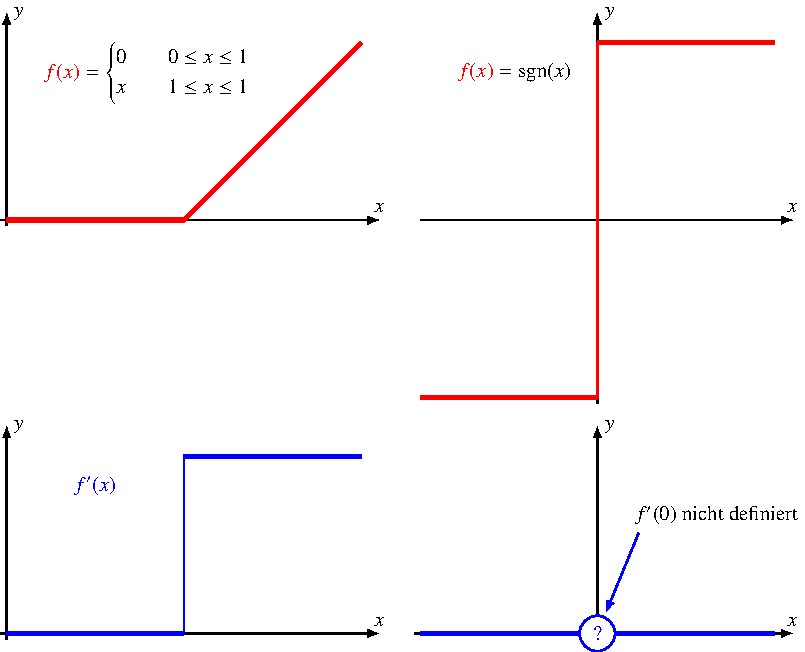
\includegraphics{chapters/010-skalarprodukt/images/schwach.pdf}
\caption{Schwache Ableitung einer nicht differenzierbaren Funktion.
Links die schwache Ableitung der Funktion von
Beispiel~\ref{buch:skalarprodukt:sobolevraum:bsp:schwachexistiert}.
Für die Signum-Funktion von
Beispiel~\ref{buch:skalarprodukt:sobolevraum:bsp:schwachexistiertnicht}
existiert die schwache Ableitung nicht, sie lässt für den Punkt $0$
nicht definieren.
\label{buch:skalarprodukt:sobolevraum:fig:schwach}}
\end{figure}
%
Die in Abbildung~\ref{buch:skalarprodukt:sobolevraum:fig:schwach} links
dargestellte Funktion
\[
f\colon (0,1) \to \mathbb{R}
:
x \mapsto
\begin{cases}
x&\qquad\text{für $0<x<1$}\\
1&\qquad\text{für $1\le x<2$}
\end{cases}
\]
ist stetig und integrierbar, aber sie ist an der Stelle $x=1$ nicht
differenzierbar.
Wir suchen die schwache Ableitung $v$ von $f$.

In einer Umgebung eines Punktes $x>1$ können wir Testfunktionen $\varphi$
so wählen, dass ihr Träger vollständig im Inneren des Intervals $(1,2)$
enthalten ist.
Mit diesen Testfunktionen können wir so rechnen, wie wenn $f$ die konstante
Funktion $1$ ist.
Das bedeutet für das Skalarprodukt
\[
\langle f,\varphi'\rangle
=
\int_1^2 \varphi'(x)\,dx
=
[\varphi(x)]_0^1 = 0.
\]
Das Skalarprodukt mit jeder beliebigen Testfunktion ist $0$, wir
müssen also $v(x)=0$ wählen.

Für $x$ im Teilinterval $(0,1)$ können wir die Testfunktionen so wählen,
dass der Träger vollständig im Inneren  von $(0,1)$ enthalten ist und
somit $f$ als die beliebig oft stetig differenzierbare Funktion $x$
behandelt werden darf.
Für das Skalarprodukt folgt dann
\[
-\langle f,\varphi'\rangle
=
-\int_0^1 f(x)\,\varphi'(x)\,dx
=
-\int_0^1 x\varphi'(x)\,dx
=
-[x\varphi(x)]_0^1 +\int_0^1 \varphi(x)\,dx
=
\langle 1,\varphi(x)\rangle,
\]
in diesem Teil des Intervals muss die schwache Ableitung den Wert $1$ 
haben.

Wir haben somit gefunden, dass die schwache Ableitung von $f$ die
Funktion
\[
v(x) = \begin{cases}
1&\qquad\text{für $0\le x<1$}
\\
0&\qquad\text{für $1< x<2$}
\end{cases}
\]
ist.
Wir kontrollieren dies, indem wir das Skalarprodukt für beliebige 
Testfunktionen $\varphi$ nachrechnen:
\begin{align*}
\langle v,\varphi\rangle
&=
\int_0^2 v(x)\,\varphi(x)\,dx
=
\int_0^1 1\,\varphi(x)\,dx
+
\int_1^2 0\,\varphi(x)\,dx.
\intertext{Jedes dieser Integrale kann man partiell integrieren:}
&=
[x\varphi(x)]_0^1 - \int_0^1 x\varphi'(x)\,dx
+
[1\varphi(x)]_1^2 - \int_1^2 1\varphi'(x)\,dx
\\
&=
\varphi(1) + \varphi(2) - \varphi(1) - \int_0^2 f(x)\,\varphi'(x)\,dx.
\intertext{Da $2$ ein Randpunkt ist, ist $\varphi(2)=0$, so dass sich}
&=-\langle f,\varphi'\rangle.
\end{align*}
ergibt.
Die Funktion $v$ ist also die schwache Ableitung von $f$.
\end{beispiel}

Eine Funktion in $W^{1,2}(\Omega)$ hat eine schwache Ableitung,
wie das Beispiel gezeigt hat, muss die Ableitung keine stetige
Funktion sein.
Ausserdem ist jede andere Funktion, die sich von der schwachen
Ableitung auf einer Menge vom Mass 0 unterscheidet, genauso eine
schwache Ableitung.
Trotzdem kann eine Funktion mit einer schwachen Ableitung nicht
beliebig ``wild'' sein, wie das folgende Beispiel zeigt.

\begin{beispiel}
\label{buch:skalarprodukt:sobolevraum:bsp:schwachexistiertnicht}
Die Signum-Funktion
\[
f\colon (-1,1) = \operatorname{sgn}(x) =
\begin{cases}
         - 1&\qquad\text{für $-1<x<0$}\\
\phantom{-}0&\qquad\text{für $x=0$}\\
\phantom{-}1&\qquad\text{für $0<x<1$}
\end{cases}
\]
ist nicht stetig (Abbildung~\ref{buch:skalarprodukt:sobolevraum:fig:schwach}).
$f$ ist fast überall konstant, in beiden Teilintervallen $(-1,0)$ und
$(0,1)$ ist die einzige mögliche schwache Ableitung von $f$ die
Nullfunktion.
Trotzdem kann $0$ nicht die schwache Ableitung von $f$ sein.
Wir wählen eine Testfunktion $\varphi$, die im Punkt $x=0$ von
Null verschieden ist.
Wäre $v$ eine schwache Ableitung von $f$, dann müsste
\begin{align*}
\langle v,\varphi\rangle
&=
-\langle f,\varphi'\rangle
=
-\int_{-1}^1 f(x) \varphi'(x)\,dx
\\
&=
-\int_{-1}^0 (-1)\cdot \varphi'(x)\,dx
-\int_{0}^1 1\cdot \varphi'(x)\,dx
=
\int_{-1}^0 \varphi'(x)\,dx
-
\int_{0}^1 \varphi'(x)\,dx
\\
&=
[\varphi(x)]_{-1}^0
-
[\varphi(x)]_{0}^1
=
\varphi(0)-\varphi(-1)
-
\varphi(1)+\varphi(0)
\\
&=
2\varphi(0)
\ne 0.
\end{align*}
Andererseits ist die Nullfunktion der einzige Kandidat für die
schwache Ableitun, für die das Skalarprodukt $\langle v,\varphi\rangle=0$
ist.
Dieser Widerspruch zeigt, dass die Funktion $f$ kein schwache
Ableitung hat.
\end{beispiel}

Die schwache Ableitung ermöglicht also mit gewissen Funktionen zu arbeiten,
die keine Ableitung im traditionellen Sinne haben.
Dank der Definition mit Hilfe eines Skalarproduktes in einem 
Hilbert-Raum darf man sich die Funktionen als Grenzwerte von
Cauchy-Folgen vorstellen.

%
% Physikalische Rechtfertigung
%
\subsection{Physikalische Rechtfertigung der schwachen Ableitung}
Die schwache Ableitung ersetzt die mit Hilfe eines Differenzenquotienten
definierte Änderungsrate durch eine Änderungsrate, die durch Vergleich
mit einer in der Umgebung eines Punktes konzentrierten Testfunktion
ermittelt wird.
Auf den ersten Blick mag das als Konzession an die Präzision der Ideen
der Analysis erscheinen, die Newton erfunden hat, um die Physik auf eine
neue Grundlage zu stellen.
Dabei wird aber vergessen, dass der Differenialquotient eine physikalisch
nicht erreichbare Idealisierung darstellt.
Keine Messung kann in einem Punkt im geometrischen Sinn erfolgen.
Die Bestimmung einer Position eines Massepunktes zum Beispiel erfolgt
durch Beobachtung des Lichtes, das vom Massepunkt reflektiert wird.
Doch der Massepunkt ist kein Punkt im geometrischen Sinn, er ist ausgedehnt
über ein endliches Gebiet.
Auch ist die Messung nicht instantan, es wird Licht gemessen, welches
über ein Zeitintervall vom Massepunkt reflektiert wird.
Das Messresultat entsteht also notwendigerweise als Mittelwert der
Beobachtung einer sehr grossen Zahl von Photonen, die von verschiedenen
Stellen reflektiert wurden.
Ein solcher Mittelwert ist genau das, was ein Skalarprodukt
$\langle f,\varphi\rangle$ mit einer Testfunktion ermittelt.

Die Feldgleichungen der Elektrodynamik wurden von Maxwell ausgehend
von Faradays Ideen als partielle Differentialgleichungen formuliert.
Sie verknüpfen die Werte des elektrischen Feldes $\vec{E}$ und des
magnetischen Feldes $\vec{B}$ mit der Ladungsdichte $\varrho$
und der Stromdichte $\vec{\jmath}$, die die Felder erzeugen.
Doch sowohl die Ladungsdichte wie auch die Stromdichte sind Idealisierungen.
Ladungen und Ströme sind nicht stetig über den Raum verteilt, sondern 
in Elektronen oder Atomkernen konzentriert.
Die Ladungsdichte entsteht daraus durch Messung der Ladung in einem kleine
Raumgebiet und Mittelung, was man wieder als Skalarprodukt mit einer
Testfunktion beschreiben kann.

Das elektrische Feld wird gemessen, indem die Kraft auf eine Testladung
im Feld ermittelt wird.
Ausser den prinzipiellen Einschränkungen an die Genauigkeit der
Positionsmessung wissen wir auch aus der Quantenmechanik, dass so etwas
wie die exakte Position eines Teilchens nicht gibt, wir können nur eine
Wahrscheinlichkeitsverteilung dafür bekommen.
Die Kraft äussert sich in einer Geschwindigkeitsänderung, die aber erst
messbar wird, wenn man die Beschleunigung eine gewisse Zeit lang aufrecht
erhält.
Das Messresultat ist also wieder ein Mittelwert über viele Positionen
und Zeitpunkte, oder anders ausgedrückt ein Skalarprodukt mit einer
Testfunktion.

Weitere Beispiele kann man auch in der Fluiddynamik finden.
Die Navier-Stokes-Gleichungen beschreiben die Strömung eines Mediums
unter der Annahme, dass es durch die Dichte $\varrho$ und die
Geschwindigkeit exakt beschreiben lässt.
Das Medium setzt sich aber aus einzelnen Atomen zusammen, die Dichte
ist also bereits ein Mittelwertbildung.
Bei der Geschwindigkeit wird das Problem noch deutlicher.
Auch die Strömungsgeschwindigkeit eines Gases ist der Mittelwert der
Strömungsgeschwindigkeit der Teilchen. 
Die Geschwindigkeit einzelner Teilchen ist dabei meistens sehr viel
grösser, nämlich im Bereich der Schallgeschwindigkeit, und äussert sich
in der Temperatur des Gases, also der mittleren kinetischen Energie.
Es ist nicht sinnvoll, von der Temperatur eines einzelnen Atoms zu
sprechen.

Alle diese Beispiele zeigen, dass die Ableitung als Änderungsrate, die
mit einem Differenzenquotienten bestimmt werden kann, eine Idealisierung
ist.
Wir können dies sogar etwas formeller zeigen.
Sei $x(t)$ die Koordinate eines Massepunktes zur Zeit $t$.
Die Messung kann nicht instantan erfolgen, im besten Fall ist die
gemessene Position ein Integral der Form
\[
\hat{x}(t)
=
\int_{-\infty}^\infty x(\tau) \varphi(\tau - t)\,d\tau.
\]
Darin ist $\varphi$ eine Testfunktion mit Träger in der Nähe von $0$.
Schreiben wir $T_t\varphi(\tau) = \varphi(\tau -t)$, dann können wir
das Messresultat auch als Skalarprodukt
$\hat{x}(t)=\langle x,T_t\varphi\rangle$
schreiben.
Die Messung mit der gleichen Aparatur einen Moment $\Delta t$ später ergibt
\[
\hat{x}(t+\Delta t)
=
\int_{-\infty}^\infty x(\tau) \varphi(\tau-t-\Delta t)\,dt
=
\langle x, T_{t+\Delta t}\varphi\rangle.
\]
Die Geschwindigkeit als Differenzenquotient ist
\begin{equation}
\frac{
\hat{x}(t+\Delta t)-\hat{x}(t)
}{\Delta t}
=
\frac{
\langle f,T_{t+\Delta t}\varphi\rangle
-
\langle f,T_{t}\varphi\rangle
}{
\Delta t
}
=
\left\langle
f,\frac{T_{t+\Delta t}\varphi - \varphi}{\Delta t}
\right\rangle
\label{buch:skalarprodukt:sobolevlraum:eqn:geschwindigkeit}
\end{equation}
Die Funktion $(T_{t+\Delta t}\varphi-T_t\varphi)/\Delta t$ ist eine 
beliebig oft stetig differenzierbare Funktion, die im Grenzwert
$\Delta t\to 0$ gegen
\[
\frac{
\varphi(\tau - t - \Delta t)
-
\varphi(\tau - t)
}{
\Delta t
}
=
-
\frac{
\varphi(\tau - t + \delta) - \varphi(\tau - t)
}{
\delta
}
\to 
-
\varphi'(\tau - t)
\quad
\text{für $\delta = - \Delta \to 0$}
\]
konvergiert.
Der Differenzenquotient
\eqref{buch:skalarprodukt:sobolevlraum:eqn:geschwindigkeit}
konvergiert daher gegen
\[
\lim_{\Delta t\to 0}
\frac{
\hat{x}(t+\Delta t)-\hat{x}(t)
}{\Delta t}
=
\left\langle
x,
\lim_{\Delta t\to 0}
\frac{T_{t+\Delta t}\varphi-T_t\varphi}{\Delta t}
\right\rangle
=
\langle f,-\varphi'\rangle
=
-
\langle f, \varphi'\rangle.
\]
Dieses einfache Modell einer ``unscharfen'' Messung führt also automatisch
auf das Konzept der schwachen Ableitung.








%\uebungsabschnitt
%\aufgabetoplevel{chapters/010-potenzen/uebungsaufgaben}
%\begin{uebungsaufgaben}
%\uebungsaufgabe{101}
%\uebungsaufgabe{102}
%\uebungsaufgabe{103}
%\uebungsaufgabe{104}
%\end{uebungsaufgaben}
%\endgroup


%
% chapter.tex -- Skalarprodukt
%
% (c) 2021 Prof Dr Andreas Müller, Hochschule Rapperswil
%
% !TeX spellcheck = de_CH
\chapter{Skalarprodukte
\label{buch:chapter:skalarprodukte}}
\kopflinks{Skalarprodukte}

%
% 1-definition.tex
%
% (c) 2023 Prof Dr Andreas Müller, OST Ostschweizer Fachhochschule
%
\section{Definition
\label{buch:opertoren:section:definition}}
\kopfrechts{Definition}


%
% 2-cauchyschwarz.tex
%
% (c) 2022 Prof Dr Andreas Müller, OST Ostschweizer Fachhochschule
%
\section{Ungleichungen
\label{buch:skalarprodukte:section:cauchyschwarz}}
\kopfrechts{Cauchy-Schwarz-Ungleichung}
In der Vektorgeometrie wird gelehrt, dass die Länge eines Vektors $u$
durch die Norm $\|u\|$ wiedergegeben wird und dass die geometrische
Intuition dazu passt.
Dazu gehört vor allem, dass die Dreiecksungleichung erfüllt ist,
dass also für drei Punkt $A$, $B$ und $C$
\begin{equation}
\overline{AB} \le \overline{AC} + \overline{BC}
\label{skalarprodukt:ungleichungen:eqn:dreieck}
\end{equation}
gilt.
In Vektorform bedeutet dies, dass
\[
\| b-a\|
\le
\| c-a\| + \|b-c\|.
\]
Schreibt man $u=c-a$ und $v=b-c$, dann ist $u+v=b-a$ und somit
\begin{equation}
\| u+v\| \le \|u\| + \|v\|.
\label{skalarprodukt:cauchyschwarz:eqn:dreieck0}
\end{equation}
Dies ist die Dreiecksungleichung in
Vektorform~\eqref{skalarprodukt:cauchyschwarz:eqn:dreieck0}.
Ziel dieses Abschnitts ist zu zeigen, dass jedes reelle oder
komplexe Skalarprodukt diese und weitere Eigenschaften automatisch
mitbringt.

%
% Cauchy-Schwarz-Ungleichung
%
\subsection{Cauchy-Schwarz-Ungleichung}
Sei also $\langle\;\,,\;\rangle$ ein reelles oder komplexes Skalarprodukt
auf dem Vektorraum $V$,
insbesondere ist $\langle v,v\rangle\ge 0$ für beliebige Vektoren $v\in V$.
Für zwei Vektoren $x,y\in V$ und $t\in \mathbb{R}$  gilt daher
\begin{align}
0
&\le
\| x+ty\|^2
=
\langle x+ty,x+ty\rangle
=
\langle x,x\rangle
+
t\langle x,y\rangle
+
t\langle y,x\rangle
+
t^2
\langle y,y\rangle.
\label{skalarprodukt:cauchyschwarz:eqn:quadrat}
\end{align}
Für ein reelles Skalarprodukt ist $\langle x,y\rangle=\langle y,x\rangle$
und damit
\begin{align}
0
&\le
\|x\|^2 + 2t\langle x,y\rangle + t^2 \|y\|^2.
\label{buch:skalarprodukt:cauchyschwarz:eqn:cspoly}
\end{align}
Dies ist ein quadratisches Polynom in der Variablen $t$, dessen Minimum
nicht negativ sein darf.

%
% Minimum eines quadratischen Polynoms
%
\subsubsection{Minimum eines quadratischen Polyoms}
Ein beliebiges quadratisches Polynom
\[
p(t)=at^2+bt+c
\]
kann durch
quadratisches Ergänzen in die Form
\[
p(t)
=
a\biggl(t+\frac{b}{2a}\biggr)^2 -\frac{b^2}{4a}+c
\]
gebracht werden.
Daraus kann man ablesen, dass das Minimum an der Stelle
\[
t_0
=
-\frac{b}{2a}
\]
angenommen wird und den Wert 
\begin{equation}
p(t_0)
=
c-\frac{b^2}{4a}
\end{equation}
hat.
Die gleiche Lösung kann natürlich auch durch Bestimmung des Minimums
von $p(t)$ mit Hilfe der Bedingung $p'(t_0)=0$ gefunden werden.

%
% Cauchy-Schwarz-Ungleichung für einen reellen Vektorraum
%
\subsubsection{Cauchy-Schwarz-Ungleichung für einen reellen Vektorraum}
Für~\eqref{buch:skalarprodukt:cauchyschwarz:eqn:cspoly}
ist
\[
a=\|y\|^2,\quad
b=2\langle x,y\rangle
\quad\text{und}\quad
c=\|x\|^2.
\]
Daher folgt aus~\eqref{buch:skalarprodukt:cauchyschwarz:eqn:cspoly}
\[
0
\le
\|x\|^2 - \frac{\langle x,y\rangle^2}{\|y\|^2}
\qquad\Rightarrow\qquad
\langle x,y\rangle^2 \le \|x\|^2\, \|y\|^2
\qquad\Rightarrow\qquad
|\langle x,y\rangle| \le \|x\|\, \|y\|.
\]
Dies ist die Cauchy-Schwarz-Ungleichung für das Skalarprodukt
$\langle \;\,,\;\rangle$.

\begin{satz}[Cauchy-Schwarz]
\label{buch:skalarprodukt:cauchy-schwarz:satz:reell}
Ein reelles Skalarprodukt $\langle\;\,,\;\rangle$ auf dem reellen Vektorraum
$V$ erfüllt die Cauchy-Schwarz-Ungleichung
\[
|\langle x, y\rangle| \le \|x\|\,\|y\|
\]
für $x,y\in V$.
\end{satz}

%
% Cauchy-Schwarz-Ungleichung für einen komplexen Vektorraum
%
\subsubsection{Cauchy-Schwarz-Ungleichung für einen komplexen Vektorraum}
Für ein komplexes Skalarprodukt ist das Produkt $\langle x,y\rangle$
nicht mehr unbedingt reell und kann damit nicht mehr direkt mit den
Normen $\|x\|^2u$ und $\|y\|^2$ vergleichen.
Wir ersetzen daher $t$ durch
$t\langle y,x\rangle=t\overline{\langle x,y\rangle}$
und erhalten 
\begin{align*}
0
\le
\|x+t\langle y,x\rangle y\|^2
&=
\langle x,x\rangle
+t\langle y,x\rangle \langle x,y\rangle
+t\overline{\langle y,x\rangle}\langle y,x\rangle
+t^2\langle y,y\rangle
\\
&=
\|x\|^2
+
t
2|\langle x,y\rangle|^2
+
t^2 |\langle x,y\rangle|^2
\|y\|^2.
\end{align*}
Dies ist wieder ein quadratisches Polynom, diesmal mit den Koeffizienten
\[
a= |\langle x,y\rangle|^2 \|y\|^2,
\quad
b= 2|\langle x,y\rangle|^2
\quad\text{und}\quad
c= \|x\|^2.
\]
Das Minimum dieses Polynoms ist nach
\[
0
\le
c-\frac{b^2}{4a}
=
\|x\|^2 - \frac{|\langle x,y\rangle|^4}{|\langle x,y\rangle|^2\,\|y\|^2}
=
\|x\|^2 - \frac{|\langle x,y\rangle|^2}{\|y\|^2}
\quad\Rightarrow\quad
|\langle x,y\rangle|^2 \le \|x\|^2\,\|y\|^2
\quad\Rightarrow\quad
|\langle x,y\rangle \le \|x\|\,\|y\|.
\]
Dies ist die Cauchy-Schwarz-Ungleichung für einen komplexen Vektorraum.

\begin{satz}[Cauchy-Satz]
\label{buch:skalarprodukt:cauchy-schwarz:satz:komplex}
Ein komplexes Skalarprodukt $\langle\;\,,\;\rangle$ auf dem komplexen Vektorraum
$V$ erfüllt die Cauchy-Schwarz-Ungleichung
\[
|\langle x, y\rangle| \le \|x\|\,\|y\|
\]
für $x,y\in V$.
\end{satz}

Man beachte, dass die
Sätze~\ref{buch:skalarprodukt:cauchy-schwarz:satz:reell}
und
\ref{buch:skalarprodukt:cauchy-schwarz:satz:komplex}
nur die Axiome eines Skalarproduktes verwenden.
Sie gelten also
ganz unabhängig von der konkreten Definition des Skalarproduktes,
solange die Eigenschaften eines Skalarproduktes gegeben sind.

\begin{beispiel}
Die sesquilineare Funktion
\[
\langle x,y\rangle
=
\sum_{i=1}^n\overline{x}_i y_i
\]
für Vektoren $x,y\in\mathbb{C}^n$ ist positiv definit, denn
\[
\langle x,x\rangle
=
\sum_{i=1}^n \overline{x}_i x_i = \sum_{i=1}^n |x_i|^2 > 0
\]
für $x\ne 0$.
Nach Satz~\ref{buch:skalarprodukt:cauchy-schwarz:satz:komplex}
gilt daher
\[
\biggl|
\sum_{i=1}^n \overline{x}_i y_i
\biggr|
\le
\sqrt{\sum_{i=1}^n |x_i|^2} \sqrt{\sum_{i=1}^n |y_i|^2}
\quad\text{oder auch}\quad
\biggl|
\sum_{i=1}^n x_i y_i
\biggr|
\le
\sqrt{\sum_{i=1}^n |x_i|^2} \sqrt{\sum_{i=1}^n |y_i|^2}
\]
für beliebige Vektoren $x,y\in\mathbb{C}^n$.
\end{beispiel}

\begin{beispiel}
Die sesquilineare Funktion
\[
\langle f,g\rangle
=
\int_a^b \overline{f(x)} g(x)\,dx
\]
für komplexwertige, stetige Funktion auf dem Intervall $[a,b]$
ist positiv definit, denn
\[
\langle f,f\rangle
=
\int_a^b \overline{f(x)} f(x)\,dx
=
\int_a^b |f(x)|^2\,dx
\ge 0
\]
für $f\ne 0$.
Nach Satz~\ref{buch:skalarprodukt:cauchy-schwarz:satz:komplex}
gilt daher
\begin{align*}
\biggl|\int_a^b \overline{f(x)}g(x)\,dx\biggr|
&\le
\sqrt{\int_a^b |f(x)|^2\,dx}
\sqrt{\int_a^b |g(x)|^2\,dx}
\intertext{oder auch}
\biggl|\int_a^b f(x) g(x)\,dx\biggr|
&\le
\sqrt{\int_a^b |f(x)|^2\,dx}
\sqrt{\int_a^b |g(x)|^2\,dx}
\end{align*}
für beliebige komplexwertige stetige Funktionen $f,g$ auf dem
Intervall $[a,b]$.
\end{beispiel}

%
% Dreiecksungleichung
%
\subsection{Dreiecksungleichung}
Die Intuition einer Längenmessung basiert auf der
Dreiecksungleichung~\eqref{skalarprodukt:ungleichungen:eqn:dreieck}.
Sie ist gleichbedeutend mit der
Vektorform~\eqref{skalarprodukt:cauchyschwarz:eqn:dreieck0}
der Ungleichung.

Die Cauchy-Schwarz-Ungleichung ermöglicht nun, diese Ungleichung
nachzurechnen.
Die Norm von $\|x+y\|^2$ ist
\[
\|x+y\|^2
=
\langle x+y,x+y\rangle
=
\langle x,x\rangle
+
\langle x,y\rangle
+
\langle y,x\rangle
+
\langle y,y\rangle
=
\|x\|^2 + 2\operatorname{Re}\langle x,y\rangle + \|y\|^2.
\]
Den mittleren Term kann man mit der Cauchy-Schwarz-Ungleichung
umformen:
\begin{align*}
\|x\|^2 + 2\operatorname{Re}\langle x,y\rangle + \|y\|^2.
&\le
\|x\|^2 + 2|\operatorname{Re}\langle x,y\rangle| + \|y\|^2.
\\
&\le
\|x\|^2 + 2|\langle x,y\rangle| + \|y\|^2.
\\
&\le
\|x\|^2 + 2\|x\|\,\|y\| + \|y\|^2
=
(\|x\| + \|y\|)^2.
\end{align*}
Durch Ziehen der Wurzel folgt
\[
\|x+y\| \le \|x\| + \|y\|.
\]
Damit ist der folgende Satz bewiesen.

\begin{satz}[Dreiecksungleichung]
Für die Norm zu einem beliebigen Skalarprodukt auf dem reellen
oder komplexen Vektorraum $V$ gilt die Dreiecksungleichung
\[
\|x+y\| \le \|x\| + \|y\|
\]
für $x,y\in V$.
\end{satz}

%
% Normen
%
\subsection{Normen
\label{skalarprodukt:cauchyschwarz:subsection:norm}}
Das Skalarprodukt ist nicht die einzige Möglichkeit, eine Norm auf
einem Vektorraum zu definieren.
Zum Beispiel kann man auf $\mathbb{C}^n$ die sogenannte $l^1$-Norm
definieren.

\begin{definition}
Die Funktion
\[
\|x\|_1
=
\sum_{i=1}^n |x_i|
\]
für $x\in\mathbb{C}^n$ heisst die {\em $l^1$-Norm} auf $\mathbb{C}^n$.
\end{definition}

Die Funktion $\|\cdot\|_1$ ist eine Norm im Sinne der folgenden Definition.

\begin{definition}
Eine Funktion $\|\cdot\| \colon V\to\mathbb{R}$ auf einem reellen
oder komplexen Vektorraum $V$ heisst eine {\em Norm}, wenn Sie die
folgenden Bedingungen erfüllt
\begin{enumerate}
\item
$\|\lambda x\| = |\lambda|\, \|x\|$ für $x\in V$ und $\lambda\in \Bbbk$
\item
Für alle Vektoren $x\in V$ mit $x\ne 0$ gilt $\|x\|>0$.
\item
Dreiecksungleichung: $\|x+y\| \le \|x\| + \|y\|$ für alle $x,y\in V$
\end{enumerate}
\end{definition}

Es ist klar, dass die $l^1$-Norm die Bedingungen~1 und 2 erfüllt.
Aber auch die Bedingung~3 kann man leicht  nachprüfen:
\[
\|x+y\|_1
=
\sum_{i=1}^n |(x+y)_i|
=
\sum_{i=1}^n |x_i+y_i|
\le
\sum_{i=1}^n(|x_i|+|y_i|)
=
\sum_{i=1}^n|x_i|
+
\sum_{i=1}^n|y_i|
=
\|x\|_1 + \|y\|_1,
\]
wozu wir nur die Dreiecksungleichung $|a+b|\le |a| + |b|$ für reelle 
oder komplexe Zahlen $a,b$ benötigen.

\begin{beispiel}
Die Funktion
\[
\|x\|_\infty = \sup_{1\le i\le n} |x_i|
\]
ist eine Norm auf $\mathbb{C}^n$.
\end{beispiel}

Auch in diesem Fall sind die Bedingungen~1 und 2 ganz offensichtlich erfüllt.
Für die Dreiecksungleichung rechnen
\begin{align*}
\|x+y\|_\infty
&=
\sup_{1\le i\le n} |x_i+y_i|
\le
\sup_{1\le i\le n} (|x_i|+|y_i|)
\le
\sup_{1\le i\le n} |x_i|+\sup_{1\le i\le n}|y_i|
=
\|x\|_\infty + \|y\|_\infty.
\end{align*}
Somit ist $\|\cdot\|_\infty$ eine Norm auf $\mathbb{C}^n$.

%
% Polaridentität
%
\subsection{Polaridentität}
Die durch das Skalarprodukt definierte Norm
\( \|x\|^2=\langle x,x\rangle \)
ist nach Abschnitt~\ref{skalarprodukt:cauchyschwarz:subsection:norm}
ein Spezialfall einer Norm.
Ist es möglich, für eine Norm, die von einem Skalarprodukt herkommt,
das Skalarprodukt wieder zu rekonstruieren?

%
% Reelles Skalarprodukt aus der Norm
%
\subsubsection{Reelles Skalarprodukt aus der Norm}
Die Antwort gibt der folgende Satz.

\begin{satz}[Polaridentität]
\label{skalarprodukt:cauchyschwarz:satz:polarformel}
Ist $\|\cdot\|$ die Norm zu einem Skalarprodukt auf dem reellen Vektorraum
$V$, dann kann das Skalarprodukt zweier Vektoren $x,y\in V$ mittels
der sogenannten {\em Polaridentität}
\index{Polaridentität}%
\begin{equation}
\langle x, y\rangle
=
\frac12\bigl(
\|x+y\|^2 - \|x\|^2 - \|y\|^2 
\bigr)
\label{skalarprodukt:cauchyschwarz:eqn:polar}
\end{equation}
berechnet werden.
\end{satz}

\begin{proof}[Beweis]
Die Gleichung
\begin{align*}
\|x+y\|^2
&=
\langle x+y,x+y\rangle
=
\|x\|^2 + 2\langle x,y\rangle + \|y\|^2 
\end{align*}
kann nach $\langle x,y\rangle$ aufgelöst werden und ergibt
die behauptete Formel~\eqref{skalarprodukt:cauchyschwarz:eqn:polar}.
\end{proof}

% 
% Parallelogrammgleichung
%
\subsubsection{Parallelogrammgleichung}
\begin{figure}
\centering
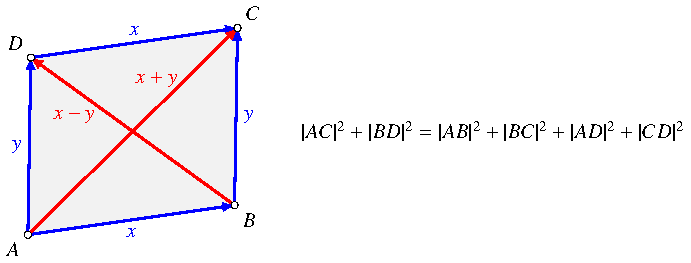
\includegraphics{chapters/010-skalarprodukt/images/parallelogramm.pdf}
\caption{Parallelogrammregel für eine Norm, die aus einem Skalarprodukt
entsteht.
\label{skalarprodukt:cauchyschwarz:fig:parallelogramm}}
\end{figure}
Die Polaridentitäten können auch noch in einer anderen Form geschrieben
werden.
Dazu berechnet man zusätzlich die Norm von $x-y$:
\begin{align*}
\|x+y\|^2
&=
\|x\|^2 + \|y\|^2 + 2\langle x, y\rangle
\\
\|x-y\|^2
&=
\|x\|^2 + \|y\|^2 - 2\langle x, y\rangle
\\
\|x+y\|^2 +\|x-y\|^2
&=
2\|x\|^2 + 2\|y\|^2
\end{align*}

\begin{satz}
\label{skalarprodukt:cauchyschwarz:satz:parallelgramm}
Für eine Norm, die von einem reellen Skalarprodukt herkommt, gilt die
Parallelogrammformel
\begin{equation}
\|x+y\|^2 +\|x-y\|^2
=
2\|x\|^2 + 2\|y\|^2.
\label{skalarprodukt:cauchyschwarz:eqn:parallelgramm}
\end{equation}
(Abbildung~\ref{skalarprodukt:cauchyschwarz:fig:parallelogramm})
\end{satz}

Das Skalarprodukt kann man damit auf verschiedene Weise aus der
Norm gewinnen:
\begin{equation}
\begin{aligned}
\langle x, y\rangle
&=
{\textstyle\frac12}\bigl( \|x\|^2 + \|y\|^2 - \|x+y\|^2 \bigr)
\\
&=
{\textstyle\frac12}\bigl(
\|x+y\|^2
-
\|x\|^2 
-
\|y\|^2
\bigr)
\\
&=
{\textstyle\frac14}\bigl(
\|x+y\|^2 - \|x-y\|^2
\bigr).
\end{aligned}
\label{skalarprodukt:cauchyschwarz:eqn:realteil}
\end{equation}
Nur die letzte Formel ist noch nicht gut begründet.
Man kann aber sofort nachrechnen, dass 
\begin{align*}
\|x+y\|^2&=\|x\|^2+2\langle x,y\rangle+\|y\|^2\\
\|x-y\|^2&=\|x\|^2-2\langle x,y\rangle+\|y\|^2
\intertext{die Differenz}
\|x+y\|^2 - \|x-y\|^2 &= 4\langle x,y\rangle
\qquad
\Rightarrow
\qquad
\langle x,y\rangle
=
\frac14\bigl(\|x+y\|^2 - \|x-y\|^2\bigr)
\end{align*}
haben.

%
% Komplexes Parallelogramm aus der Norm
%
\subsubsection{Komplexe Skalarprodukt}
Das Resultat von Satz~\ref{skalarprodukt:cauchyschwarz:satz:polarformel}
gilt in abgeänderter Form auch für komplexe Skalarprodukte.
Da das Skalarprodukt auch einen nichtverschwindenen Imaginärteil haben
kann, wird eine zusätzliche Gleichung zur Berechnung des Imaginärteils
nötig.
Eine solche kann gewonnen werden, indem zusätzlich die Normen
$\|x+iy\|^2$ und $\|x-iy\|^2$ berechnet werden.
Dazu ist zu beachten, dass
\[
\langle x,y\rangle
-
\langle y,x\rangle
=
\langle x,y\rangle
-
\overline{
\langle x,y\rangle
}
=
2i\operatorname{Im}\langle x,y\rangle
\]
Damit erhält man
\begin{align*}
\|x+iy\|^2 &= \|x\|^2 + i\langle x,y\rangle - i\langle y,x\rangle + \|y\|^2 
           = \|x\|^2 + 2\operatorname{Im}\langle x,y\rangle + \|y\|^2 \\
\|x-iy\|^2 &= \|x\|^2 - i\langle x,y\rangle + i\langle y,x\rangle + \|y\|^2 
           = \|x\|^2 - 2\operatorname{Im}\langle x,y\rangle + \|y\|^2.
\end{align*}
Damit kann man nach dem Imaginärteil des Skalarproduktes auflösen und
die Formeln
finden, die den Formeln
\eqref{skalarprodukt:cauchyschwarz:eqn:realteil}
für das reelle Skalarprodukt entsprechen.
\eqref{skalarprodukt:cauchyschwarz:eqn:realteil}
Formeln bleiben gültig als Formeln für den Realteil des Skalarproduktes.
Damit haben wir den folgenden Satz gefunden.

\begin{satz}[Polaridentitäten für ein komplexes Skalarprodukt]
Ist $\|\cdot\|$ die Norm, die aus dem komplexen Skalarprodukt
$\langle\;\,,\;\rangle$ auf einem Vektorraum $V$ gewonnen wurde,
dann können Real- und Imaginärteil mit den Formeln
\begin{align*}
\operatorname{Re}\langle x,y\rangle
&=
{\textstyle\frac12}\bigl(
\|x+y\|^2 - \|x\|^2 -\|y\|^2
\bigr)
\\
&=
{\textstyle\frac12}\bigl(
\|x\|^2 +\|y\|^2 - \|x+y\|^2
\bigr)
\\
&=
{\textstyle\frac14}\bigl(
\|x+y\|^2 - \|x-y\|^2
\bigr),
\\
\operatorname{Im}\langle x,y\rangle
&=
{\textstyle\frac12}\bigl(
\|x+iy\|^2-\|x\|^2-\|y\|^2
\bigr)
\\
&=
{\textstyle\frac12}\bigl(
\|x\|^2+\|y\|^2-\|x-iy\|^2
\bigr)
\\
&=
{\textstyle\frac14}\bigl(
\|x+iy\|^2
-
\|x-iy\|^2
\bigr)
\end{align*}
für beliebige Vektoren $x,y\in V$
allein aus Werten der Norm berechnet werden.
\end{satz}


%
% 3-funktionenraeume.tex
%
% (c) 2022 Prof Dr Andreas Müller, OST Ostschweizer Fachhochschule
%
\section{Funktionenräume
\label{buch:skalarprodukt:section:funktionenraeume}}
\kopfrechts{Funktionenräume}
Ziel der harmonischen Analysis ist die effiziente Approximation einer
grossen Klasse von Funktionen.
Als approximierende Funktionen kommen stetige Funktionen, Polynome,
trigonometrische Polynome oder eine ähnlich, einfach konstruierbare
Funktionenfamilie in Frage.
Es gilt zunächst herauszufinden, was ``Approximation'' genau heissen
soll und von welchen Funktionen man überhaupt erwarten kann, dass sie
approximiert werden können.

%
% Stetige Funktionen
%
\subsection{Stetige Funktionen
\label{buch:skalarprodukt:subsection:stetige-funktionen}}
Der frühe intuitive Funktionsbegriff ging oft von der Vorstellung einer
in einem Strich gezeichneten Kurve aus, wie man sie von den Graphen
der Polynome oder der trigonometrischen Funktionen her kennt.
In moderner Sprechweise sind dies die stetigen Funktionen.

\begin{definition}
Eine Funktion $f\colon I\to\mathbb{R}$ mit $I\subset \mathbb{R}$
heisst stetig in einem Punkt $x_0\in I$, wenn für jedes $\varepsilon>0$
ein $\delta>0$ existiert derart, dass $f(x)-f(x_0)|<\delta$ sobald
$|x-x_0|<\varepsilon$.
\end{definition}

Nur die Eigenschaft, eine Abstandsmessung zu besitzen, wird vom
Definitionsbereich $I\subset \mathbb{R}$ verlangt.
Der Stetigkeitsbegriff kann daher verallgemeinert werden auf den
Begriff des metrischen Raumes.

\begin{definition}
Eine {\em Metrik} auf einer Menge $X$ ist eine Funktion
\index{Metrik}%
$d\colon X\times X\to \mathbb{R}$
mit den folgenden Eigenschaften
\begin{enumerate}
\item
Positiv definit: $d(x,y)\ge 0$ und $d(x,y)$ genau dann, wenn $x=y$.
\item
Symmetrie: \(d(x,y)=d(y,x)\)
\item
Dreiecksungleichung: \( d(x,y) \le d(x,z) + d(z,y) \).
\end{enumerate}
Ein {\em metrischer Raum} ist ein Menge $X$ mit einer Metrik.
\index{matrischer Raum}%
\end{definition}

In einem metrischen Raum ist der Begriff des Grenzwertes übertragbar.
Mit dem Begriff des Grenzwertes lässt sich auch der Begriff der
Stetigkeit verallgemeinern.

\begin{definition}
Ist $x_n\in X$ eine Folge von Punkten in einem metrischen Raum $X$,
dann heisst $x$ der Grenzwert der Folge $x_n$, wenn es für jedes
$\varepsilon>0$ ein $N>0$ gibt derhart, dass
$d(x_n,x)\le \varepsilon$ für alle $n>N$.
Eine Funktion $f\colon X\to Y$ zwischen metrischen Räumen heisst
stetig im Punkt $x\in X$, wenn für jede Folge $x_n\in X$ mit
Grenzwert $x$ auch die Folge $y_n=f(x_n)\in Y$ konvergiert und
den Grenzwert $y=f(x)$ hat.
\end{definition}

Teilmengen von $\mathbb{R}$ oder $\mathbb{R}^n$ tragen natürlich
die Struktur eines metrischen Raumes mit der Abstandsmessung in 
$\mathbb{R}^n$ als Metrik
\[
d(x,y) = \sqrt{(x_1-y_1)^2 + \ldots + (x_n-y_n)^2} = \|x-y\|.
\]
Die Eigenschaften einer Metrik wurden bereits in Abschnitt
\ref{buch:skalarprodukte:section:cauchyschwarz} nachgewiesen.

Der Begriff des Grenzwertes klärt, was mit der Approximation von $x$
durch eine Folge $x_n$ gemeint ist.
Wenn man darauf aufbauend die Konvergenz einer Folge von Funktionen
gegen eine Grenzfunktion definieren will, braucht man einen Abstansbegriff
zwischen Funktionen.
Ein erster Versuch könnte sein, als Abstand zwischen zwei Funktionen
$f$ und $g$ die Funktion
\[
d(f,g) = |f(x_0) - g(x_0)|.
\]
Die Menge der Funktionen wird dadurch jedoch nicht zu einem metrischen
Raum.
Zwar gilt sicher die Symmetrie und Dreiecksungleichung, und auch 
$d(f,g)\ge 0$ für beliebige Funktionen.
Aber wenn $d(f,g)=0$ ist, heisst das nur, dass $f$ und $g$ im Punkt
$x_0$ den gleichen Wert haben.
Ausser in trivialen Fällen wird es Funktionen geben, die zwar im Punkt
$x_0$ übereinstimmen, sich aber in mindestens einem anderen Punkt
unterscheiden.

%
% Normierte Räume
%
\subsubsection{Normierte Räume}
Die stetigen Funktionen bilden aber keine strukturlose Menge, sie
bilden einen Vektorraum: die Summe von stetigen Funktionen ist ebenfalls
stetig, multiplizieren einer stetigen Funktion mit einem Skalar führt
nicht aus der Menge der stetigen Funktionen heraus.
Die für den Grenzwertbegriff von Funktionen verwendete Abstandsmessung 
sollte der Vektorraumstruktur ebenfalls Rechnung tragen.

\begin{definition}
\label{buch:skalaprodukt:funktionenraume:def:norm}
Sei $V$ ein Vektorraum über $\mathbb{R}$, dann heisst eine Funktion
\( \|\;\cdot\;\| \colon V \to \mathbb{R}\) eine {\em Norm}, wenn gilt
\index{Norm}
\begin{enumerate}
\item
Definit: $ \|x\| = 0 \Rightarrow x=0$
\item
Homogeneität: $ \| \lambda x \| = |\lambda| \cdot \|x\|$
\item
Dreiecksungleichung: $\|x+y\| \le \|x\| + \|y\|$
\end{enumerate}
Ein {\em normierter Raum} ist ein Vektorraum $V$ mit einer Norm.
\end{definition}

%
% Vollständigkeit
%
\subsubsection{Vollständigkeit}
In den rationalen Zahlen hat nicht jede Folge einen Grenzwert.
Die Zahl $\sqrt{2}$ lässt sich beliebig genau durch rationale Zahlen
approximieren, sie ist aber nicht in $\mathbb{Q}$.
Ähnlich lässt sich die Funktion $x\mapsto \sqrt{x}$ beliebig genau 
durch Polyome approximieren, sie ist aber selbst kein Poylnome

\begin{definition}
Ein Folge $x_n\in X$ in einem metrischen Raum heisst {\em Cauchy-Folge},
wenn es für jedes $\varepsilon>0$ ein $N>0$ gibt derart, dass 
$|x_n-x_m|<\varepsilon$ wenn $n,m>N$ ist.
\end{definition}

Cauchy-Folgen sind also Folgen, die sich für genügend grossen Index
kaum mehr ändern und für die man daher Konvergenz erwarten würde.

\begin{definition}
Ein normierter Raum heisst {\em vollständig} oder ein Banach-Raum,
wenn jede Cauchy-Folge einen Grenzwert hat.
\end{definition}

Die rationalen Zahlen $\mathbb{Q}$ bilden keinen vollständigen
metrischen Raum, aber die reellen Zahlen $\mathbb{R}$ enthalten
alle Grenzwerte von Cauchy-Folgen, $\mathbb{R}$ ist eine vollständiger
metrischer Raum.
Die Menge der Polynome, betrachtet als Teilmenge der Menge der
stetigen Funktionen $[0,1]\to\mathbb{R}$ ist nicht vollständig,
da es eine Folge $f_n(x)$ von Approximationsfunktionen der Funktion
$x\mapsto \sqrt{x}$ gibt.
Als Cauchy-Folge konvergiert sie zwar gegen eine stetige Funktion,
aber die Grenzfunktion ist nicht mehr im Raum der Polynome.

Das Ziel der folgenden Kapitel ist also, zu geeignet interessanten
Funktionenfamilien ``gute'' Normen zu finden derart, dass Cauchy-Folgen
konvergieren gegen Funktionen, die immer noch ausreichend viele
nützliche Eigenschaften haben.
Im besten Fall konvergieren stetige Funktionen gegen stetige Funktionen,
es wird sich aber zeigen, dass diese Anforderung zu streng ist.

%
% Norm fpr stetige Funktionen
%
\subsection{Norm für stetige Funktionen
\label{buch:skalarprodukt:subsection:normfuerstetigefunktionen}}
Damit man von Konvergenz von Folgen stetiger Funktionen sprechen kann,
brauchen wir jetzt also eine Norm für stetige Funktionen.

\begin{definition}
Sei $X$ ein metrischer Raum und
\[
C(X)
=
C_{\mathbb{R}}(X)
=
\{
f\colon X \to\mathbb{R}\mid
\text{$f$ ist stetig}
\}
\]
der Vektorraum der stetigen Funktion auf $X$.
Die Norm von $C(X)$ ist definiert als
\[
\|f\| = \sup_{x\in X} |f(x)|.
\]
Sie heisst die {\em Supremum-Norm}.
\end{definition}

Wir prüfen nach, dass die Supremum-Norm tatsächlich eine Norm ist.
Dazu sind die definierenden Eigenschaften nachzurechnen:
\begin{enumerate}
\item Definit: 
\[
0
=
\|f\|
=
\sup_{x\in X} |f(x)|
\quad\Rightarrow\quad
f(x)=0 \;\forall x\in X
\quad\Rightarrow\quad
f\in C(X).
\]
\item Homogeneität:
\[
\|\lambda f\|
=
\sup_{x\in X} |\lambda f(x)|
=
|\lambda| \sup_{x\in X} |f(x)|
=
|\lambda| \cdot \|f\|.
\]
\item
Dreiecksungleichung:
\[
\|f+g\|
=
\sup_{x\in X}|f(x)+g(x)|
\le
\sup_{x\in X}(|f(x)|+|g(x)|)
\le
\sup_{x\in X}|f(x)|+\sup_{x\in X}|g(x)|
=
\|f\| + \|g\|.
\]
\end{enumerate}

Eine Cauchy-Folge $f_n$ von Funktionen $X\to \mathbb{R}$ hat die
Eigenschaft, dass für jedes $\varepsilon >0$ ein $N>0$ existiert,
derart dass $\|f_n-f_m\|<\varepsilon$ ist.
Da die Norm der maximale Unterschied von Funktionswerten ist,
folgt dass für eine Cauchy-Folge in $C(X)$ die Folge $f_n(x)$ eine
Cauchy-Folge in $\mathbb{R}$ ist und damit einen Grenzwert in $\mathbb{R}$
hat.
Die Funktion $f(x) = \lim_{n\to\infty}f_n(x)$ ist die Grenzfunktion.
Die Konvergenz bezüglich der Norm besagt, dass für jedes $\varepsilon>0$
es ein $N>0$ gibt derart, dass
\[
\varepsilon 
>
\|f_n-f\|
\ge 
|f_n(x)-f(x)|
\]
ist für alle $n>N$ und unabhängig von $x\in X$.
Die Konvergenz bezüglich der $\|\;\cdot\;\|$-Norm ist also die wohlbekannte
gleichmässige Konvergenz.
Es kann gezeigt werden, dass die Grenzfunktion wieder stetig ist.

\begin{satz}
Der Raum der stetigen Funktion $C(X)$ mit der Supremumg-Norm ist
ein Banach-Raum.
\end{satz}

%
% Skalarprodukt
%
\subsection{Skalarprodukt
\label{buch:skalarprodukt:subsection:skalarprodukt}}
\begin{figure}
\centering
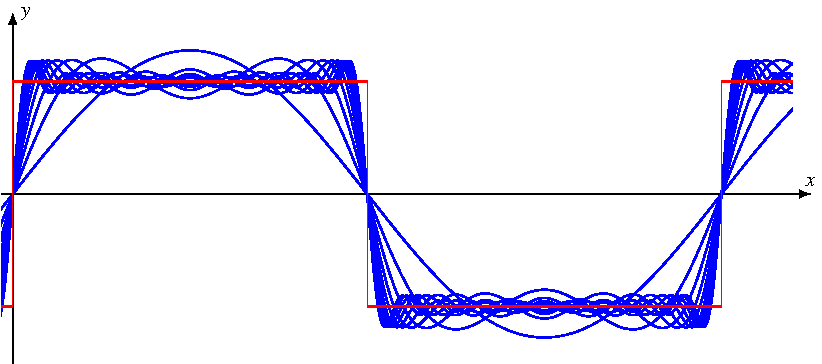
\includegraphics{chapters/010-skalarprodukt/images/fourierrechteck.pdf}
\caption{Approximation der Rechteckfunktion (rot) durch eine Folge
von Partialsummen der Fourier-Reihe.
\label{buch:skalarprodukt:fig:fourierrechteck}}
\end{figure}%
Die Supremum-Norm auf dem Raum der stetigen Funktionen hat den
Begriff der gleichmässig konvergenten Funktionenfolgen ergeben.
Cauchy-Folgen von stetigen Funktionen in der Supremum-Norm konvergieren
wieder gegen eine stetige Funktione.
Ist eine Funktion nicht stetig, lässt Sie sich im Sinne der Supremum-Norm
nicht durch stetige Funktionen approximieren.
Andererseits hat Fourier gezeigt, wie man technische wichtige Funktionen
wie die Rechteckfunktion durch trigonometrische Polynome
\begin{equation}
f_n(x)
=
\frac{4}{\pi} \sum_{k=0}^n \frac{\sin kx}{k}
=
\frac{4}{\pi} \biggl(
\sin x
+
\frac{\sin 3x}{3}
+
\frac{\sin 5x}{5}
+
\frac{\sin 7x}{7}
+
\ldots
\biggr)
\label{buch:skalarprodukt:eqn:rechteckreihe}
\end{equation}
approximieren kann.
Diese sind alle stetig und kommen der Rechteckfunktion in jedem Punkt,
in dem die Funktion stetig ist, beliebig nahe.
An den Stellen $x = n\pi$ hat die Grenzfunktion eine Sprungstelle,
die approximierenden Funktionen haben dort immer Abstand $1$
(siehe Abbildung~\ref{buch:skalarprodukt:fig:fourierrechteck}).
Die Folge ist also keine Cauchy-Folge und sie konvergiert nicht im
Sinne der Supremum-Norm.
Für solche Anwendungen muss eine besser geeignete Norm gefunden werden,
in der die Folge konvergiert.

%
% Skalarprodukt von Funktion
%
\subsubsection{Die $L^1$-Norm einer Funktion}
Die Supremum-Norm sieht nur den grössten Wert, die Konvergenz der Folge
\eqref{buch:skalarprodukt:eqn:rechteckreihe} ist aber nicht gleichmässig,
die maximale Abweichung ist immer $1$.
Gesucht ist eine Norm, die für die Folge
\eqref{buch:skalarprodukt:eqn:rechteckreihe} 
nur im Mittel eine Abweichung feststellt.
Für die Berechnung des Mittelwerts kann das Integral verwendet werden:

\begin{definition}
\label{buch:skalaprodukt:definition:l1norm}
Für eine stetige Funktion $X\to\mathbb{R}$, für die $x\mapsto |f(x)|$
integrierbar ist, heisst
\begin{equation}
\|f\|_1 = \int_X |f(x)|\,dx
\label{buch:skalarprodukt:eqn:l1norm}
\end{equation}
die {\em $L^1$-Norm} der Funktion $f$.
\end{definition}

Die $L^1$-Norm ist tatsächlich eine Norm, wir verifizieren die
definierenden Eigenschaften einer Norm.
\begin{enumerate}
\item
Definit: Sei $f$ eine stetige Funktion mit $\|f\|_1=0$
Wäre $f\ne 0$, dann gäbe es einen Punkt $x_0\in X$ mit $f(x_0) \ne 0$.
Da $f$ stetig ist, ist $f|(x)| > \frac12|f(x_0)|$ für $x$ in einer
$\delta$-Umgebung von $x_0$.
Dann folgt für die $L^1$-Norm
\begin{align*}
\|f\|_1
=
\int_X |f(x)|\,dx
\ge
\frac12 |f(x_0)| \cdot \delta 
> 0.
\end{align*}
Dies widerspricht der Annahme, dass $\|f\|_1=0$ ist, also muss $f=0$ sein.
\item
Homogeneität folgt durch direkte Rechnung
\[
\|\lambda f\|_1
=
\int_X |\lambda f(x)|\,dx
=
|\lambda|
\int_X |f(x)|\,dx
=
|\lambda| \cdot \|f\|.
\]
\item
Die Dreiecksungleichung folgt aus
\[
\|f+g\|_1
=
\int_X |f(x) + g(x)|\,dx
\le
\int_X |f(x)| + |g(x)|\,dx
=
\int_X |f(x)| + \int_X |g(x)|\,dx
=
\|f\|_1 + \|g\|_1.
\]
\end{enumerate}

Die $L^1$-Norm ist etwas ``schwächer'' als die Supremum-Norm im
folgenden Sinne.
Eine in der Supremum-Norm konvergente Funktionenfolge auf einem
kompakten Definitionsbereich $X$ ist auch in der $L^1$-Norm konvergent.
Zur Unterscheidung der verschiedenen Normen werden wir in Zukunft die
Supremum-Norm manchmal auch als $\|f\|_{\infty} = \|f\|$ schreiben.

\begin{satz}
Ist $X$ eine kompakte Teilmenge von $\mathbb{R}$ und $f_n$ eine
in der Supremum-Norm konvergente Folge stetiger Funktionen $f_n$,
dann ist $f_n$ auch in der $L^1$-Norm konvergent.
\end{satz}

\begin{proof}
Konvergenz in der Supremum-Norm bedeutet, dass für jedes $\varepsilon>0$
ein $N>0$ existiert derart, dass $|f_n(x)-f(x)|<\varepsilon$ für alle
$x\in X$ und alle $n>N$.
Für die $L^1$-Norm gilt dann
\begin{align*}
\|f_n-f\|_1
&=
\int_X |f_n(x) - f(x)|\,dx
\le
\int_X \varepsilon \,dx
=
\varepsilon \int_X \,dx
=
\varepsilon \operatorname{vol}(X).
\end{align*}
Da für einen kompakten Definitionsbereich $\operatorname{vol}(X)<\infty$
gilt, bedeutet dies, dass die $\|f_n-f\|_1\to 0$, dass also $f_n$ in
der $L^1$-Norm konvergiert.
\end{proof}

\begin{beispiel}
Die Folge $f_n(x)$ von \eqref{buch:skalarprodukt:fig:fourierrechteck}
konvergiert tatsächlich in der $L^1$-Norm auf dem Intervall $[0,2\pi]$.
Zwar ist $f_n$ nicht gleichmässig konvergent, aber fast.
Man kann zeigen, dass für jedes $\delta>0$, die Funktionen
$f_n(x)$ in Punkten $x$, die weiter als $\delta$ von den
Punkten $k\pi$ mit $k\in\mathbb{Z}$, gleichmässig konvergieren.
Innerhalb einer $\delta$-Umgebung der Vielfachen von $\pi$ ist die
$f_n(x)-f(x)$ beschränkt.
Die genaue Schranke ist nicht wichtig, wir nennen sie $M$ und bekommen
\[
|f_n(x)-f(x)|
\le M
\quad\forall x\in X.
\]
Ausserhalb einer kleinen Umgebung konvergiert die Folge gleichmässig,
zu jedem $\varepsilon>0$ gibt es also ein $N>0$ derart, dass
\[
|f_n(x)-f(x)|<\varepsilon
\]
für $x$ weiter als $\delta$ von $k\pi$ entfernt.
Für die $L^1$-Norm folgt dann
\begin{align*}
\|f_n-f\|_1
&=
\int_0^{2\pi} |f_n(x)-f(x)|\,dx
\\
&=
\int_0^\delta |f_n(x)-f(x)|\,dx
+
\int_\delta^{\pi-\delta} |f_n(x)-f(x)|\,dx
+
\int_{\pi-\delta}^{\pi+\delta} |f_n(x)-f(x)|\,dx
\\
&\qquad
+
\int_{\pi+\delta}^{2\pi-\delta} |f_n(x)-f(x)|\,dx
+
\int_{2\pi-\delta}^{2\pi} |f_n(x)-f(x)|\,dx
\\
&\le
\delta M
+
\varepsilon (\pi -2\delta)
+
2\delta M
+
\varepsilon (\pi -2\delta)
+
\delta M
\le
4\delta M + 2\pi\varepsilon
\end{align*}
für $n>N$.
Dadurch, dass man $\delta$ und $\varepsilon$ klein macht, kann man
also immer ein $N$ finden, so dass $\|f_n-f\|_1$ beliebig klein wird
für $n>N$.
Damit ist gezeigt, dass die Folge $f_n$ in der $L^1$-Norm konvergiert.
\end{beispiel}

Das Beispiel zeigt, dass die $L^1$-Norm eine schwäre Form der Konvergenz
ist, die eine erweiterte Klasse von Funktionen durch stetige Funktionen
zu approximieren erlaubt.

%
% Das $L^2$-Skalarprodukt
%
\subsubsection{Das $L^2$-Skalarprodukt}
Die $L^1$-Norm ist weniger strikt als die Supremum-Norm, aber sie ist
immer noch recht weit von der Intuition entfernt, die wir von der
Entfernungsmessung in der Geometrie haben, die von einem Skalarprodukt
herrühren.
Das Beispiel~\ref{buch:skalarprodukt:cauchyschwarz:beispiel:skalarprodukt}
weist den Weg, mit dem wir eine Norm für stetige Funktionen gewinnen
können, die von einem Skalarprodukt herkommt.

\begin{definition}
\label{buch:skalarprodukt:funktionraeume:definition:skalarprodukt}
Das {\em Skalarprodukt} stetiger Funktionen auf $X\subset \mathbb{R}$
ist definiert durch
\begin{equation}
\langle f,g\rangle
=
\int_X f(x)g(x)\,dx.
\label{buch:skalarprodukt:funktionraeume:eqn:skalarprodukt}
\end{equation}
\end{definition}

Es genügt nachzurechnen, dass $\langle f,g\rangle$ die Eigenschaften
eines Skalarproduktes hat, dann folgt die Dreiecksungleichung automatisch.
Zunächst ist klar,
dass~\eqref{buch:skalarprodukt:funktionraeume:eqn:skalarprodukt}
bilinear ist:
\begin{align*}
\langle \lambda f_1+\mu f_2,g\rangle
=
\int_X (\lambda f_1(x) + \mu f_2(x)) g(x)\,dx
&=
\lambda\int_Xf_1(x)g(x)\,dx + \mu\int_X f_2(x)g(x)\,dx
\\
&=
\lambda\langle f_1,g\rangle + \mu\langle f_2,g\rangle
\\
\langle f,\lambda g_1+\mu g_2\rangle
=
\int_X f(x)(\lambda g_1(x)+\mu g_2(x))\,dx
&=
\lambda\int_X f(x)g_1(x)\,dx + \mu\int_X f(x)g_2(x)\,dx
\\
&=
\lambda\langle f,g_1\rangle + \mu\langle f,g_2\rangle.
\end{align*}
Die Bilinearform ist aber auch positiv definit: Für eine stetige
Funktion $f(x)$ gilt
\[
\langle f,f\rangle
=
\int_X f(x)^2\,dx \ge 0.
\]
Da auch $f(x)^2$ eine stetige Funktion ist,
verschwindet das Integral genau dann, wenn $f(x)=0\;\forall x\in X$ ist.

Die zum Skalarprodukt gehörige Norm 
\[
\|f\|_2
=
\int_X |f(x)|^2\,dx
\]
heisst auch die {\em $L^2$-Norm}.

%
% Nicht kompakte Definitionsbereiche
%
\subsubsection{Nicht kompakter Definitionsbereich}
Für stetige Funktionen auf einem kompakten Definitionsbereich scheinen
die drei Normen $\|\;\cdot\;\|_\infty$, $\|\;\cdot\;\|_1$ und
$\|\;\cdot\;\|_2$ zu den gleichen Konvergenzbegriffen zu führen.
In diesem Abschnitt soll gezeigt werden, dass dies für nicht kompakte
Definitionsbereiche nicht mehr gilt.
Nicht einmal die Menge der Funktionen, die eine endliche Norm haben,
ist gleich.

\begin{beispiel}
Auf dem Definitionsbereich $X=(0,1]$ hat die Funktion
$f(x)=\log x$ endliche $L^1$-Norm aber unendliche Supremum-Norm.

\medskip
\noindent
Wegen $\lim_{x\to 0+}\log x = -\infty$ folgt $\|\log\|=\infty$.
Für die $L^1$-Norm folgt mit der Substitution $y=\log x$ und
$dy = dx/x$ oder $dx = e^y\,dy$
\begin{align*}
\|\log\|_1
&=
\int_0^1|\log x|\,dx
=
-\int_0^1\log x\,dx
=
-\int_{-\infty}^0 e^y\,dy
=
-\biggl[ e^y \biggr]_0^{-\infty}
=
1.
\end{align*}
Insbesondere ist die $L^1$-Norm beschränkt.
\end{beispiel}

\begin{beispiel}
Auf dem Definitionsbereich $X=[1,\infty)$ hat die Funktion
$f(x)=1/x$ endliche $L^2$-Norm aber unendlich $L^1$-Norm.

\medskip
\noindent
Die Integrale für die Normen ergeben:
\begin{align*}
\|f\|_1
&=
\int_1^\infty \frac{1}{x}\,dx
&
\|f\|_2^2
&=
\int_1^\infty \frac{1}{x^2}\,dx
\\
&=\biggl[\log x\biggr]_1^\infty
&
&=\biggl[-\frac{2}{x}\biggr]_1^\infty
\\
&=\infty
&
&=2.
\end{align*}
Insbesondere ist die $L^1$-Norm unbeschränkt, die $L^2$-Norm dagegen
beschränkt.
\end{beispiel}

\begin{satz}
Eine stetige Funktion auf einem beschränkten Definitionsbereich $X$
mit endlicher $L^2$-Norm hat auch endliche $L^1$-Norm.
\end{satz}

\begin{proof}[Beweis]
Aus der Cauchy-Schwarz-Ungleichung folgt
\begin{align*}
\int_X |f(x)|\,dx
&=
\langle |f|, 1\rangle
\le
\|f\|_2\cdot \|1\|_2.
\end{align*}
Nach Voraussetzung an die Funktion $f$ ist der erste Faktor beschränkt,
der zweite Faktor ist $\operatorname{vol}(X)$ und nach Voraussetzung
auch beschränkt.
\end{proof}

Die Beispiele zeigen, dass die Existenz der Normen selbst für stetige
Funktionen für nicht kompakten Definitionsbereich nicht garantiert ist.
Die Erweiterung auf nicht stetige Funktionen kann muss daher beschränkt
werden auf eine Klasse von Funktionen, für die die entsprechende Norm
existiert.
Das kann bedeuten, dass nicht alle stetigen Funktionen in Betracht 
kommen und dass neue Funktionen, die nicht stetig sind, als
Grenzwerte auftreten können.

%
% Grenzen des Riemann-Integrals
%
\subsection{Grenzen des Riemann-Integrals}
In den vorangegangenen Rechnungen sind wir immer vom Riemann-Integral
ausgegangen, welches man im Analysisunterricht als erstes kennenlernt.
Man zeigt dort, dass es für stetige Funktionen existiert und für
gleichmässig konvergente Folgen von Funktionen der Grenzwert des
Integrals mit dem Integral des Grenzwertes übereinstimmt:
\[
\int_X \lim_{n\to\infty} f_n(x)\,dx
=
\lim_{n\to\infty}
\int_X f_n(x)\,dx
\]
Der vorangegangene Abschnitt hat gezeigt, dass wir die Klasse der
Funktionen ausdehnen müssen auf Funktionen, die nicht stetig sind,
für die aber immer noch die $L^1$- oder die $L^2$-Norm existiert.
Hier zeigen sich die Schwächen des Riemann-Integrals.
In diesem Abschnitt soll an Beispielen gezeigt werden, was schief
gehen kann, und wie das Problem gelöst werden kann.

%
% Abzählbar viele Stetigkeitsstellen
%
\subsubsection{Abzählbar viele Unstetigkeitsstellen}
Wir konstruieren eine Funktionenfolge von Riemann-integrierbaren 
Funktionen, die alle das Integral $0$ haben, deren Grenzfunktion
aber nicht mehr Riemann-integrierbar ist.

Die rationalen Zahlen im Intervall $[0,1]$ sind abzählbar, d.~h.~es
gibt eine Folge $n\mapsto q_n\in[0,1]\cap\mathbb{Q}$, in der jede
rationale Zahl im Intervall vorkommt.
Aus der Folge $q_n$ konstruieren wir jetzt die Folge von Funktionen
\[
f_n(x)
=
\begin{cases} 
1&\qquad\text{$x$ ist einer der Werte $q_1,q_2,\ldots,q_n$}\\
0&\qquad\text{sonst}.
\end{cases}
\]
Die Funktion $f_n(x)$ ist also an genau $n$ Stellen von $0$ erschieden
und hat dort den Wert $1$.
Das Riemann-Integral ``sieht'' endlich viele Sprungstellen nicht,
die Funktionen $f_n$ sind also alle Riemann-integrierbar und haben
das Integral
\[
\int_0^1 f_n(x)\,dx=0.
\]
Insbesondere ist auch
\[
\lim_{n\to\infty}\int_0^1 f_n(x)\,dx = 0.
\]
Andererseits ist die Grenzfunktion
\begin{equation}
f(x)
=
\begin{cases}
1&\qquad\text{$x\in[0,1]\cap\mathbb{Q}$ ist rational}\\
0&\qquad\text{sonst, $x$ ist irrational.}
\end{cases}
\label{buch:skalarprodukt:funktionenraeume:eqn:ratfunk}
\end{equation}
Das Riemann-Integral der Funktion $f(x)$ existiert nicht.
Dazu müsste man ja für eine Unterteilung $0=x_0<x_1<\dots x_n=1$
die Riemann-Summen
\[
\overline{I}
=
\sum_{k=0}^{n-1}
(x_{k+1}-x_k) \sup_{x_k\le \xi \le x_{k+1}} f(\xi)
\qquad\text{und}\qquad
\underline{I}
=
\sum_{k=0}^{n-1}
(x_{k+1}-x_k) \inf_{x_k\le \xi \le x_{k+1}} f(\xi)
\]
berechnen, und sie müssten bei Verfeinerung der Unterteilung
gegeneinander konvergieren.
Aufgrund der Konstruktion der Funktion $f(x)$ ist aber
\[
\sup_{x_k\le \xi \le x_{k+1}} f(\xi) = 1
\qquad\text{und}\qquad
\inf_{x_k\le \xi \le x_{k+1}} f(\xi) = 0,
\]
sodass
$\overline{I}=1$ und $\underline{I}=0$ ist, ganz unabhängig von
der Unterteilung.

Der Riemannsche Integralbegriff muss also für die Zwecke der Approxmation
mit der $L^1$ oder $L^2$-Norm erweitert werden, so dass er sinnvoll mit
abzählbar vielen Unstetigkeitsstellen umgehenn kann.
Insbesondere sollte er als Integral der Funktion $f(x)$ 
von \eqref{buch:skalarprodukt:funktionenraeume:eqn:ratfunk}
den Wert $0$ liefern.

%
% Masse
%
\subsubsection{Masstheorie}
Gesucht wird also ein Integral, das für eine grössere Klasse von
Funktionen definiert ist und welches sich bezüglich Grenzwerten
besser verhält als das Riemann-Integral.
Das Integral ist nur dann nützlich, wenn es für viele Funktionen
die gleichen Werte ergibt.

Die einfachsten Funktionen, die wir integrieren wollen, sind die
{\em Indikatorfunktionen}, Funktionen, die durch eine Teilmenge
\index{Indikatorfunktion}
$A\subset X$ definiert sind durch
\[
1_A(x)
=
\begin{cases}
1&\qquad\text{für $x\in A$}\\
0&\qquad\text{sonst}.
\end{cases}
\]
Für ein Intervall der Länge $\lambda(A)$ ist
\[
\int_X 1_A(x)\,dx = \lambda(A).
\]
Für Mengen, die sich aus vielen Intervallen zusammensetzen, erwarten wir
die Summenformel
\[
A=\bigcup_{k=1}^\infty A_k,
\quad
A_k\cap A_j = \emptyset\;\forall k\ne j
\qquad\Rightarrow\qquad
\lambda(A) = \sum_{k=1}^\infty \lambda(A_k).
\]
Ausserdem sollte für eine Teilmenge $A\subset B$ der Inhalt der
Differenz $\lambda(A\setminus B)=\lambda(A)-\lambda(B)$ sein.

So entsteht eine Klasse von Mengen, denen sinnvoll ein Inhalt 
zugeordnet werden kann.
Solche Mengen heissen {\em messbar}.
Dazu gehören alle Intervalle, aber auch alle Differenzen und
abzählbaren Vereinigungen von Intervallen und messbaren Mengen
sind wieder messbar.
Die Klasse der messbaren Mengen ist also sehr gross.
Es braucht natürlich noch einiges an Arbeit, um zu zeigen, dass
eine widerspruchsfreie Definition der Funktion $\lambda(A)$
tatsächlich möglich ist, die jeder messbaren Menge einen
Inhalt zuordnet.
Eine solche Funktion heisst ein {\em Mass}, das aus der Intervalllänge
konstruierte Mass heisst auch das Lebesgue-Mass nach Henri Léon Lebesgue..
\index{Lebesgue-Mass}%
\index{Mass}%

Von besonderem Interesse sind Mengen, deren Inhalt $0$ ist.

\begin{definition}
\label{buch:skalarprodukt:funktionenraeume:definition:nullmenge}
Eine Nullmenge bezüglich des Masses $\lambda$ ist eine messbare
Menge $A$ mit Mass $\lambda(A)=0$.
\index{Nullmenge}
\end{definition}

Der Riemannsche Integralbegriff lässt bei der Bestimmung des Masses
nur endlich viele Intervalle zu. 
Die Menge $Q$ der rationalen Zahlen im Intervall $[0,1]$ ist abzählbar
unendlich.
In jeder beliebigen Umgebung einer reellen Zahl in $[0,1]$ findet man
rationale Zahlen in $Q$, eine Überdeckung der Menge der rationalen
Zahlen mit endlich vielen Intervallen enthält daher immer auch alle
reellen Zahlen, mit der möglichen Ausnahme von endlich vielen Zahlen.
Der Inhalt, den der Riemannsche Integralbegriff der Menge $Q$ zuordnen
muss, ist daher $1$.

Der neue Massbegriff erlaubt, die Menge mit abzählbar vielen messbaren
Mengen zu überdecken.
Sei $q_k$ eine Folge, die alle rationalen Zahlen in $Q$ durchläuft.
Zu jedem $k$ konstruieren wir das Intervall
\[
A_k = (q_k-\varepsilon2^{-k},q_k+\varepsilon2^{-k})
\]
mit Inhalt $\lambda(A_k) = 2\varepsilon2^{-k}$.
Es ist klar, dass die Intervalle $A_k$ die ganze Menge $Q$ überdecken,
also
\[
Q\subset \bigcup_{k=1}^\infty A_k.
\]
Der Inhalt der Menge $Q$ ist daher
\[
\lambda(Q)
\le
\sum_{k=1}^\infty \lambda(A_k)
=
\sum_{k=1}^\infty 2\varepsilon 2^{-k}
=
2\varepsilon
\sum_{k=1}^\infty 2^{-k}
=
2\varepsilon.
\]
Da $\varepsilon$ beliebig klein gewählt werden kann, folgt, dass
$\lambda(Q)=0$ sein muss.
Aus diesem Beispiel lässt sich erahnen, dass der Lebesguesche Massbegriff
mit Grenzwerten besser umgehen kann als der aus dem Riemannschen Integral
abgeleitete.

%
% Lebesgue-Integral
%
\subsubsection{Lebesgue-Integral}
Aus der Konstruktion eines Masses $\lambda$ kann jetzt die Konstruktion
eines Integrals an die Hand genommen werden.
Dazu werden Funktionen durch Stufenfunktionen approximiert, die
von der Form
\[
f(x) = \sum_{k=1}^\infty a_k 1_{A_k}(x)
\]
sind, wobei $A_k$ messbare Mengen sind.
Für solche Funktionen ist die naheliegende Definition des Integrals
\[
\int_X f(x)\,d\lambda(x)
=
\sum_{k=1}^\infty a_k \lambda(A_k).
\]
Der wesentliche Unterschied zur Riemannsschen Konstruktion ist,
dass nicht nur Intervalle zulässig sind sondern beliebige messbare Mengen.
Die Berechnung des Inhalts einer messbaren Mengen beinhaltet bereits
die Möglichkeit, Grenzwerte zu bilden.
Auch hier ist viel Arbeit notwendig um nachzuweisen, dass sich aus diesem
Ansatz ein widerspruchsfreier neuer Integralbegriff ergibt.
Das so konstruierte Integral heisst das {\em Lebesgue-Integral} und
\index{Lebesgue-Integral}%
wird zur Unterscheidung vom gewöhnlichen Riemannschen Integral und
wegen der Bedeutung des Masses $\lambda$, welches eine grosse Rolle
bei seiner Konstruktion spielt mit
\[
\int_X f(x) \,d\lambda(x)
\]
bezeichnet.

Beim Riemannschen Integral haben endliche Mengen und Mengen mit endlich
vielen Häufungspunkten Inhalt $0$.
Viele abzählbare Mengen haben dagegen positiven Inhalt.
Das Lebesguesche Mass gibt allen abzählbaren Mengen den Inhalt 0.

Unterscheiden sich zwei Funktionen $f$ und $g$ nur auf einer Nullmenge,
sagt man, sie seien {\em fast überall} gleich, geschrieben
\[
f(x) = g(x) \qquad \text{fast überall}.
\]
Zwei fast überall gleiche Funktionen haben das gleiche Integral, denn
\[
\int_X f(x)\,dx - \int_X g(x)\,dx
=
\int_X f(x)-g(x)\,dx
=
\int_X 0\,dx=0
\]
weil das Integral einer fast überall verschwindenden Funktion $0$ ist.

%
% Funktionsklassen
%
\subsubsection{Klassen von fast überall gleichen Funktionen}
Verwendet man die mit dem Lebesgque-Integral berechnete $L^1$- oder
$L^2$-Norm, dann können Funktionen nicht voneinander unterschieden werden,
die fast überall gleich sind.
Grenzwerte von Funktionenfolgen in der $L^1$- oder $L^2$-Norm sind
daher nur bis auf eine Nullmenge bestimmt.

\begin{definition}
Die Menge der Lebesgue-integrierbaren Funktionen auf dem Definitionsbereich
$X\subset\mathbb{R}$ wird mit
\[
\mathscr{L}^1(X)
=
\mathscr{L}^1_{\mathbb{R}}(X)
=
\left\{ f\colon X\to \mathbb{R}
\;\left|\;
\text{$f$ ist $\lambda$-integrierbar und $\int_X|f(x)|\,dx< \infty$}
\right.\right\}
\]
bezeichnet.
Entsprechend besteht $\mathscr{L}^2(X)$ aus den Funktionen $X\to \mathbb{R}$,
für die $|f(x)|^2$ integrierbar ist.
Sie heissen auch die {\em quadratintegrierbaren} Funktionen.
\end{definition}

Das Lebesgue-Integral kann Funktionen, die sich nur auf einer Nullmenge
verschieden sind, nicht unterscheiden. 
Daher ist es notwenig, solche Funktionen in Klassen zusammenzufassen:

\begin{definition}
Die Relation
\[
f\sim g
\qquad:\Leftrightarrow \qquad f(x) = g(x)\quad\text{fast überall}
\]
ist eine Äquivalenzrelation.
Die Menge der Äquivalenzklassen von Funktionen in $\mathscr{L}^1(X)$
bezüglich dieser Relation werden mit $L^1(X)$ bezeichnet, ebenso werden
die Äquivalenzklassen von $\mathscr{L}^2(X)$ bezüglich der Relation $\sim$
mit $L^2(X)$ bezeichnet.
\end{definition}

Mit den Funktionsklassen in $L^1(X)$ und $L^2(X)$ lässt sich genau
so rechnen, wie man es sicht gewohnt ist.
Für die Summe von Funktionen $f_1\sim f_2$ und $g_1\sim g_2$ gilt
\[
\left.
\begin{aligned}
f_1(x)&=f_2(x)&&\text{fast überall}\\
g_1(x)&=g_2(x)&&\text{fast überall}\\
\end{aligned}
\quad
\right\}
\qquad
\Rightarrow
\qquad
f_1(x)+g_1(x) = f_2(x)+g_2(x)\quad\text{fast überall},
\]
denn die Menge, auf der sich $f_1+f_2$ und $g_1+g_2$ unterscheiden
ist höchstens die Vereinigung der Mengen, auf denen sich $f_1$ und 
$f_2$ bzw.~$g_1$ und $g_2$ unterscheiden.
Die Vereinigung von Nullmengen ist aber wieder eine Nullmenge.

%
% Lebesgue-Integral
%
\subsubsection{Dominierte Konvergenz}
Die Entwicklung des Lebesgueschen Integrallbegriffs war motiviert
vom Wunsch, ein Integral zu erhalten, welches sich bezüglich
Konvergenz von Funktionenfolgen besser verhält.
Tatsächlich liefert die Theorie den folgenden zentralen Satz.

\begin{satz}[Dominierte Konvergenz]
\label{buch:skalarprodukt:satz:dominierte-konvergenz}
Sei $f_n$ eine auf dem Definitionsbereich $X$ punktweise konvergente
Folge Lebesgue-integrierbarer Funktionen mit Grenzfunktion 
\[
f(x) = \lim_{n\to \infty} f_n(x).
\]
Sei ausserdem $g$ eine Lebesgue-integrierbare Funktion mit
$|f_n(x)|<g(x)$ für alle $x\in X$.
Dann ist $f$ Lebesgue-integrierbar und es gilt
\[
\lim_{n\to\infty} \int_X f(x)\,d\lambda(x)
=
\int_X f(x)\,d\lambda(x)
\]
\end{satz}

Der Satz der dominierten Konvergenz von Lebesgue ersetzt also die
Bedingung der gleichmässigen Konvergenz, die beim Riemann-Integral
erfolgreich war, durch die viel schächere Bedingung, dass alle
Funktionen unterhalb einer gemeinsamen integrierbaren Funktion bleiben.
Dadurch wird verhindert, dass die Funktionen $f_n$ nach $\infty$
``ausbrechen'' kann und gegen eine Funktion konvergieren, die nicht
mehr integrierbar ist.


%
% Berechnung von Lebesgue-Integralen
%
\subsubsection{Berechnung von Lebesgue-Integralen}
Das Lebesque-Integral löst also die technischen Probleme, die das
Riemann-Integral manchmal bei Funktionenfolgen hat, die gegen ein
Grenzfunktion konvergieren, der man ein sinnvolles Integral im
Lebesgueschen Sinnen zuordnen kann.
Doch wie berechnet man ein Lebesgue-Integral?

Stetige Funktionen lassen sich beliebig genau durch Treppenfunktionen
approximieren.
Die Konvergenz des Lebesgue-Integrals für solche Funktionenfolgen
garantiert daher, dass das Lebesgue-Integral für stetige
Funktionen mit dem Riemann-Integral übereinstimmt.
Insbesondere braucht es keinen neuen Formalismus für die 
Berechnung von Integralen.
Auch für Funktionen, die an höchstens endlich vielen Stellen unstetig
sind, stimmt das Riemann-Integral mit dem Lebesgue-Integral überein.

Man soll sich daher das Lebesgue-Integral vor allem als eine 
Erweiterung des Integrals auf Funktionen vorstellen, die als Grenzwerte
von Folgen stetiger Funktionen im Sinne der $L^1$- oder der $L^2$-Norm
auftreten können.
Stetigkeit kann dabei verloren gehen, aber Konvergenzeigenschaften
wie die dominierte Konvergenz von
Satz~\ref{buch:skalarprodukt:satz:dominierte-konvergenz}
bleiben erhalten.




%
% 4-hilbertraum.tex
%
% (c) 2022 Prof Dr Andreas Müller, OST Ostschweizer Fachhochschule
%
\section{Hilbert-Raum
\label{buch:skalarprodukt:section:hilbertraum}}
\kopfrechts{Hilbert-Raum}
Ein Skalarprodukt stattet einen Vektorraum mit einer Norm aus.
Es ermöglicht auch, orthonormierte Vektoren zu finden.
In endlichdimensionalen Vektorräumen können so besonders nützliche
Basen konstruiert werden.
In den Funktionenräumen von
Abschnitt~\ref{buch:skalarprodukt:section:funktionenraeume},
die unendlichdimensional sind, kann der Orthonormalisierungsprozess
ohne Ende weitergeführt werden.
Im Gegensatz zu einem endlichdimensionalen Vektorraum bilden diese
orthonormierten Vektoren keine Basis, denn nicht jeder Vektor lässt
sich als Linearkombination schreiben.
Dies wird erst mit Hilfe von Reihenentwicklungen möglich, doch dazu
müssen Fragen der Konvergenz solcher Reihen geklärt werden.
Der in diesem Abschnitt eingeführte Begriff des Hilbert-Raumes tut dies.

%
% Prähilbertraum
%
\subsection{Prähilbertraum}
Die Funktionenräume, in denen wir harmonische Analysis betreiben wollen,
zeichnen sich durch das Vorhandensein eines Skalarproduktes aus.
Wir fassen diese Eigenaschaften im Begriff des Prähilbertraumes
zusammen.

\begin{definition}
Ein reeller Prähilbertraum ist ein reller Vektorraum mit einem
(reellen) Skalarprodukt.
\index{Prähilbertraum}%
Eine komplexer Prähilbertraum ist ein komplexer Vektorraum mit einem
sesquilinearen Skalarprodukt.
\end{definition}

\begin{beispiel}
Der endlichdimensionale reelle Vektorraum $\mathbb{R}^n$ ist ein
reller Prähilbertraum mit dem Skalarprodukt
\[
\langle u,v\rangle
=
\sum_{i=1}^n u_iv_i
\]
für Vektoren $u,v\in\mathbb{R}^n$.
\end{beispiel}

\begin{beispiel}
Der endlichedimensionale komplexe Vektorrau $\mathbb{C}$ ist ein
komplexer Prähilbertraum mit dem Skalarprodukt
\[
\langle u,v\rangle
=
\sum_{i=1}^n \overline{u}_iv_i
\]
für Vektoren $u,v\in\mathbb{C}^n$.
\end{beispiel}

Die Skalarprodukte in den Beispielen sind nicht die einzig möglichen
Skalarprodukte.
Alternative Skalarprodukte auf einem reellen Prähilbertraum können 
durch eine beliebige positiv definite Matrix $A$ durch
\[
\langle u,v\rangle_A
=
\sum_{i,j=1}^n u_ia_{ij}v_j
\]
definiert werden.
Wir schreiben die aus $\langle\;,\;\rangle_A$ abgeleitete Norm mit
$\normfunc_A$.
Solange unser primäres Interesse der Approximation von Funktionen gilt,
kommt es vor allem darauf an, dass die Norm, die aus dem Skalarprodukt
abgeleitet wird, zu den gleichen konvergenten Folgen führen.
Die Funktion $u\mapsto \|u\|_A$ ist stetig, sie hat daher auf der
Einheitskugel des Prähilbertraumes ein Maximum und eine Minimum,
welches wir mit $M$ bzw.~$m$ bezeichen.
Dann folgt, dass
\[
m\|u\|\le \|u\|_A\le M\|u\|
\]
für beliebige Vektoren $u\in\mathbb{R}^n$.
Daraus kann man jetzt ableiten, dass die beiden Normen $\normfunc$
und $\normfunc_A$ auf die gleichen Cauchy-Folgen und die gleichen
konvergenten Folgen führen.
Wir zeigen dies für Cauchy-Folgen:
\begin{enumerate}
\item
Sei $u_k$ eine Cauchy-Folge bezüglich der Norm $\normfunc$,
und $\varepsilon>0$.
Wir müssen zeigen, dass $u_k$ auch eine Cauchy-Folge ist bezüglich
der Norm $\normfunc_A$.
Da $u_k$ eine Cauchy-Folge bezüglich der Norm $\normfunc$ ist,
gibt es ein $N>0$ derart, dass
$\|u_k-u_l\|<\varepsilon/M$ für $k,l>N$.
Dann folgt aber
\[
\|u_k-u_l\|_A
\le
M\|u_k-u_l\|
<
M\frac{\varepsilon}{M}
=
\varepsilon
\]
für $k,l>N$.
Somit ist $u_k$ eine Cauchy-Folge bezüglich der Norm $\normfunc_A$.
\item
Ist umgekehrt  $u_k$ eine Cauchy-Folge bezüglich der Norm $\|\,\cdot\,\|_A$,
dann gibt es ein $N>0$ derart, dass $\|u_k-u_l\|_A<m\varepsilon$ ist für
$k,l>N$.
Dann folgt
\[
m\|u_k-u_l\|\le \|u_k-u_l\|_A < m\varepsilon
\qquad\Rightarrow\qquad \|u_k-u_l\|<\varepsilon
\]
für $k,l>N$, also ist $u_k$ auch eine Cauchy-Folge bezüglich der Norm
$\|\,\cdot\,\|$.
\end{enumerate}
In einem endlichdimensionalen Prähilbertraum hat die Wahl des Skalarproduktes
keinen Einfluss darauf, ob eine Folge eine Cauchy-Folge ist oder nicht.
Orthonormierte Vektoren werden natürlich im Allgemeinen nicht mehr
orthonormiert, dies ist jedoch ein Aspekt, dem wir uns erst später
zuwenden werden.

%
% Orthonormierte Vektoren
%
\subsection{Orthonormierte Vektoren in einem Prähilbertraum}
Der Gram-Schmidt-Orthogonalisierungsprozess kann auf eine beliebige
\index{Gram-Schmidt}%
linear unabhängige Menge von Vektoren in einem Prähilbertraum angewendet
werden.
Aus den linear unabhängigen Vektoren $a_1,a_2,\dots$ werden die
orthonormierten Vektoren
\begin{align*}
b_1
&=
\frac{a_1}{\|a_1\|}
\\
b_2
&=
\frac{
a_2 - \langle b_1,a_2\rangle b_1
}{
\|a_2 - \langle b_1,a_2\rangle b_1\|
}
\\
&\phantom{i}\vdots
\\
b_n
&=
\frac{\displaystyle
a_n - \sum_{k=1}^{n-1} \langle b_k,a_n\rangle b_k
}{\displaystyle
\biggl\|a_n - \sum_{k=1}^{n-1} \langle b_k,a_n\rangle b_k\biggr\|
}.
\end{align*}

In einem endlichdimensionalen Vektorraum der Dimension $n$ bricht
der Prozess ab, sobald eine orthonormierte Basis $b_1,\dots,b_n$
aus $n$ Vektoren gefunden wurde.
Jeder andere Vektor $v$ lässt sich dann als Linearkombination
\begin{equation}
v
=
\langle b_1,v\rangle b_1 + \langle b_2,v\rangle b_2 + \dots
=
\sum_{k=1}^n \langle b_1,v\rangle b_1
\label{buch:skalarprodukt:hilbertraum:synthese}
\end{equation}
schreiben.
Da die Summe auf der rechten Seite endlich ist, entstehen keine
Bedenken bezüglich Konvergenz, wie das bei einer unendlichen
Reihe der Fall wäre.

%
% Vollständigkeit
%
\subsection{Vollständigkeit}
In einem unendlichdimensionalen Prähilbertraum bricht der
Orthogonalisierungsprozess nicht ab, es gibt immer noch einen
linear unabhängigen Vektor, der nicht in dem von den bereits
gefundenen Vektoren aufgespannten Raum liegt.
Die Summe~\ref{buch:skalarprodukt:hilbertraum:synthese} wird dann
eine unendliche Summe, die nur im Sinne eines Grenzwertes der
Partialsummenfolge
\begin{equation*}
s_n = \sum_{k=1}^n \langle b_k,v\rangle b_k
\end{equation*}
ausgewertet werden kann.
Man darf zwar aufgrund der Konstruktion aus $v$ davon ausgehen,
dass $s_n$ gegen $v$ konvergiert,
aber für eine beliebige Folge von Koeffizienten $c_k$ ist nicht
garantiert, dass die Summe
\[
\sum_{k=1}^\infty c_kb_k
=
\lim_{n\to\infty} \sum_{k=1}^n c_kb_k
\]
einen Grenzwert hat.
Ein nützliche Theorie kann nur entstehen, wenn gefordert wird,
dass jede Cauchy-Folge des Prähilbertraums tatschächlich konvergiert.

\begin{definition}
Ein Prähilbertraum heisst {\em Hilbert-Raum}, wenn er vollständig ist.
\end{definition}

Endlichdimensionale Vektorräume über sind automatisch vollständig,
da gibt es also gar keinen Unterschied zwischen Prähilbertraum und
Hilbert-Raum.
Das folgende Beispiel zeigt, dass dies für unendlichdimensionale
Hilbert-Räume nicht mehr zutrifft.

\begin{beispiel}
\label{buch:skalarprodukt:hilbertraum:bsp:sinreihe}
Der Funktionenraum
\(
C_{\mathbb{R}}([-\pi,\pi])
\)
der stetigen Funktionen auf dem Intervall $[-\pi,\pi]$ wird mit
dem Skalarprodukt
\[
\langle f,g\rangle
=
\int_{-\pi}^\pi f(x)g(x)\,dx
\]
zu einem Prähilbert-Raum.
Die Summanden der Reihe~\eqref{buch:skalarprodukt:eqn:rechteckreihe} 
sind Sinus-Funktionen, von denen wir später zeigen werden, dass sie
orthogonal sind.
Seien $s_n(x)$ die Partialsummen der Reihe, also
\begin{equation}
s_n(x) = \frac{4}{\pi}\sum_{k=0}^n \frac{\sin (2k+1)x}{2k+1},
\label{buch:skalarprodukt:hilbertraum:eqn:sn}
\end{equation}
dann kann man auch die Norm $\|s_n-s_m\|$, es gilt nämlich
\begin{equation}
\|s_n-s_m\|
=
\biggl\|
\frac{4}{\pi}
\sum_{k=m}^n \frac{\sin (2k+1)x}{2k+1}
\biggr\|,
\label{buch:skalarprodukt:hilbertraum:eqn:snsm}
\end{equation}
wobei wir $n>m$ angenommen haben, was wir ohne Beschränkung der 
Allgemeinheit tun dürfen.
Die Norm eines einzeln Terms ist
\begin{align}
\|\sin rx\|^2
&=
\int_{-\pi}^\pi \sin^2 rx\,dx
=
\int_{-\pi}^\pi \frac12 - \frac{\cos rx}{2}\,dx
=
\int_{-\pi}^\pi \frac12\,dx - \int_{-\pi}^\pi \frac{\cos rx}{2}\,dx.
\notag
\intertext{Der zweite Term ist ein Integral über eine Periode des
Integranden und verschindet daher.
Der erste Term ergibt daher}
\|\sin rx\|^2
&= \pi.
\intertext{Für die Terme der Summe
\eqref{buch:skalarprodukt:hilbertraum:eqn:sn}
folgt daher}
\biggl\|
\frac{\sin{2k+1}x}{2k+1}
\biggr\|^2
&=
\frac{\pi}{(2k+1)^2}.
\notag
\intertext{Für die Differenz
\eqref{buch:skalarprodukt:hilbertraum:eqn:snsm} finden wir daher}
\|s_n-s_m\|^2
\notag
&=
\frac{16}{\pi^2}
\sum_{k=m}^m \frac{\pi}{(2k+1)^2}
=
\frac{16}{\pi}
\sum_{k=m}^m \frac{1}{(2k+1)^2}.
\label{buch:skalarprodukt:hilbertraum:eqn:bsprest}
\end{align}
Da aus dem Analysisunterricht bekannt ist, dass die Reihe $\sum_k\frac1{k^2}$
konvergiert, kann die rechte Seite von 
\eqref{buch:skalarprodukt:hilbertraum:eqn:bsprest}
beliebig klein gemacht werden, die 
Reihe~\eqref{buch:skalarprodukt:eqn:rechteckreihe} 
ist also eine Cauchy-Folge im Prähilbertraum $C_{\mathbb{R}}([-\pi,\pi])$.
Die Grenzfunktion ist die Rechteckfunktion von
Abbildung~\ref{buch:skalarprodukt:fig:fourierrechteck}, sie ist nicht
stetig.
Wir haben also eine Cauchy-Folge im Prähilbertraum 
$C_{\mathbb{R}}([-\pi,\pi])$ gefunden, die darin nicht konvergiert.
\end{beispiel}

%
% Hilbert-Basis
%
\subsection{Hilbert-Basis}
Sei jetzt $H$ ein Hilbert-Raum.
Führt man wieder die Konstruktion einer orthonormierten Basis durch,
entsteht eine Menge $\mathcal{B}=\{b_1,b_2,\dots\}$ orthonormierter
Vektoren.
In einem unendlichdimensionalen Hilbert-Raum ist $\mathcal{B}$ eine
undendliche Menge.
Die Vollständigkeit des Hilbert-Raumes garantiert, dass jede
Cauchy-Folge konvergiert, insbesondere können wir zu jedem beliebigen
Vektor $v$ die Koeffizienten $c_k=\langle b_k,v \rangle$ bestimmen
und versuchen, mit der
Summe~\eqref{buch:skalarprodukt:hilbertraum:synthese}
den Vektor zurückzugewinnen.
Vollständigkeit garantiert zwar die Konvergenz gegen einen Grenzwert
\[
v_0 = \sum_{k=1}^\infty c_k b_k,
\]
aber es gibt keine Garantie, dass $v=v_0$ ist.

\begin{beispiel}
Die Funktionen
\[
b_k(x) = \sin (2k+1)x
\qquad\text{mit}\quad
k\in \mathbb{N}
\]
wurden in Beispiel~\ref{buch:skalarprodukt:hilbertraum:bsp:sinreihe}
die Rechteckfunktion synthetisiert.
Doch reichen diese Funktionen nicht aus, um alle Funktionen auf
dem Intervall $[-\pi,\pi]$ zu synthetisieren.

Für die konstante Funktion $v(x)$ sind die Koeffizienten
\[
\langle v,b_k\rangle
=
\int_{-\pi}^\pi v(x)b_k(x)\,dx
=
\int_{-\pi}^\pi \sin (2k+1)x\,dx
=
0,
\]
die Summe
\[
v_0
=
\sum_{k=0}^\infty
c_k
b_k(x)
=
0
\]
verschwindet also, $v\ne v_0$.
\end{beispiel}

Wir berechnen das Skalarprodukt 
\[
\langle v-v_0,b_k\rangle
=
\langle v,b_k\rangle
-
\biggl\langle \sum_{l=1}^\infty c_lb_l,b_k\biggr\rangle
=
c_k - \sum_{l=1}^\infty c_l\langle b_l,b_k\rangle
=
c_k - \sum_{l=1}^\infty c_l\delta_{lk}
=
c_k-c_k=0.
\]
Der Vektor $v-v_0$ muss also orthogonal sein zu allen Vektoren
$b_k$.
Die Menge der Vektoren $b_k$ kann also vergrössert werden um einen
weiteren Vektor, der zu allen vorhandenen Vektoren orthogonal ist.

\begin{satz}
Eine Menge von orthogonalen Vektoren in einem Prähilbertraum ist linear 
unabhängig.
\end{satz}

\begin{proof}[Beweis]
Angenommen, die orthogonalen Vektoren  $a_1,\dots,a_n$ sind linear
abhängig.
Dann gibt es Zahlen $\lambda_i$, die nicht alle $=0$ sind und derart,
dass
\[
\sum_{k=1}^n \lambda_ka_k
=
\lambda_1 a_1 + \ldots + \lambda_n a_n
=
0.
\]
Das Skalarprodukt mit $a_k$ ergibt
\[
0
=
\langle a_k,\lambda_1a_1 +\ldots + \lambda_na_n\rangle
=
\lambda_1
\langle a_k,a_1\rangle
+
\ldots
+
\lambda_n
\langle a_k,a_n\rangle
=
\lambda_k \|a_k\|^2
\]
für alle $k=1,\dots,n$.
Da die Vektoren $a_k\ne 0$ sind folgt, dass $\lambda_k=0$ sein muss
für alle $k=1,\dots,n$, im Widerspruch zur Voraussetzung, dass die
$\lambda_k$ nicht alle verschwinden.
Der Widerspruch zeigt, dass die Annahme der linearen Abhängigkeit
falsch ist.
\end{proof}

In einem endlichdimensionalen Prähilbertraum findet man immer eine
orthonormierte Basis, aus der sich jeder Vektor linear kombinieren
lässt.
In einem unendlichdimensionalen Raum muss dieser Begriff etwas 
erweitert werden.

\begin{definition}
Eine {\em Hilbert-Basis} des Hilbert-Raumes $H$ ist eine Menge von orthonormalen
\index{Hilbert-Basis}%
Vektoren $b_k\in H$, $k\in \mathbb{N}$ derart, für jeden Vektor $v\in H$
die Reihe 
\[
\sum_{k\in\mathbb{N}} \langle b_k,v\rangle b_k
\]
konvergiert und die Summe $v$ hat.
\end{definition}

Auf eine Hilbert-Basis ist die Inuition anwendbar, die man von 
einer orthonormierten Basis eines endlichdimensionalen Prählibertraumes
hat.

\begin{definition}
\index{separabel}%
Ein Hilbert-Raum, der eine Hilbert-Basis besitzt, heisst {\em separabel}.
\end{definition}

Nicht separable Hilbert-Räume sind deutlich grösser.
In einem nicht separable Hilbert-Raum ist es nicht möglich, alle Vektoren
aus einer Folge von orthonormierten Vektoren linear zu kombinieren.
Dies verträgt sich nicht mit der Intuition, die in endlichdimensionalen
Vektorräumen entstanden ist.
Separabilität ist eine Art ``Endlichkeitseigenschaft''.
Man findet sie zum Beispiel bei den $L^2$-Räumen mit kompaktem
Definitionsgebiet.
Kompaktheit kann als eine topologische
Endlichkeitseigenschaft angesehen werden.
Es lassen sich aber auch nicht separable Hilbert-Räume konstruieren,
zum Beispiel sogenannte fastperiodische Funktionen.
\index{fastperiodische Funktionen}%
Für unsere Anwendungen sind nicht separable Hilbert-Räume jedoch nicht
notwendig und wir können im folgenden annehmen, dass alle Hilbert-Räume
separabel sind und somit eine Hilbert-Basis haben.

%
% Der Hilbert-Raum $l^2$
%
\subsection{Der Hilbert-Raum $l^2$}
Die abstrakte Definition eines separablen Hilbert-Raumes suggeriert,
dass es sehr viele verschiedene Hilbert-Räume geben könnte.
Dem ist aber nicht so, ein Hilbert-Raum ist eine ziemlich starre Struktur.
In diesem Abschnitt konstrieren wir zunächst den besonders übersichtlichen
separablen Hilbert-Raum $l^2$ und zeigen anschliessend, dass sich jeder
separable Hilbert-Raum isometrisch auf $l^2$ abbilden lässt.

\begin{satz}
Der Vektorraum der unendlichen Folgen
\[
l^2_{\mathbb{R}}
=
\biggl\{
(x_0,x_1,\dots)
\in
\mathbb{R}^{\mathbb{N}}
\,\bigg|\,
\sum_{i=0}^\infty x_i^2<\infty\biggr\}
\}
\]
mit dem Skalarprodukt
\[
\langle x,y\rangle_2
=
\sum_{k=0}^\infty x_ky_k
\]
ist ein separabler Hilbert-Raum.
\end{satz}

\begin{proof}[Beweis]
Die Standardbasis des Vektorraums $l^2$ besteht aus den Vektoren $e_i$
mit $i\in\mathbb{N}$ mit 
\begin{align*}
e_0 &= (1,0,0,0,\dots)
\\
e_1 &= (0,1,0,0,\dots)
\\
e_2 &= (0,1,0,0,\dots)
\\  &\;\vdots
\end{align*}
Es ist klar, dass die Vektoren $e_i$ orthonormiert sind.
Wir müssen uns überlegen, dass jede Folge in $l^2$ durch Linearkombinationen
approximiert werden kann.
Wäre das nicht so, dann gäbe es einen von $0$ verschiedenen
Vektor $v=(v_0,v_1,v_2,\dots)\in l^2$, der auf allen Vektoren $e_i$
orthogonal ist.
Dann wäre aber $0=\langle v,e_i\rangle = v_i$, d.~h.~Vektor $v$ ist der
Nullvektor.
Dieser Widerspruch zeigt, dass die Vektoren $e_i$ eine Hilbert-Basis
bilden.
\end{proof}

Der Hilbert-Raum $l^2$ ist die einfachste, direkte Verallgemeinerung der
endlichdimensionalen Hilbert-Raume $\mathbb{R}^n$ mit dem Standardskalarprodukt.
Er ist aber auch der ``einzige'' separable Hilbert-Raum, alle Hilbert-Räume
lassen sich isometrisch auf $l^2$ abbilden.

\begin{satz}
\label{buch:skalarprodukt:hilbertraum:satz:phil2}
Ist $H$ ein separabler Hilbert-Raum, dann gibt es eine isometrische
lineare Abbildung $\varphi\colon H\to l^2$.
\end{satz}

\begin{proof}[Beweis]
Da $H$ separabel ist, gibt es eine Hilbert-Basis $b_0,b_1,b_2,\ldots\in H$
und $v$ ein beliebiger Vektor mit der Darstellung
\[
v = \sum_{k=0}^\infty c_kb_k.
\]
Das Skalarprodukt mit $b_k$ ist
\[
\langle b_i,v\rangle
=
\biggl\langle b_i,\sum_{k=0}^\infty c_kb_k\biggr\rangle
=
\sum_{k=0}^\infty c_k \underbrace{\langle b_i,b_k\rangle}_{\delta_{ik}}
=
c_i.
\]
Die Abbildung
\[
\varphi\colon H \to l^2
:
v \mapsto (\langle b_0,v\rangle,\langle b_1,v\rangle,\langle b_2,v\rangle,\dots)
=
(c_0,c_1,c_2,\dots)=c\in l^2
\]
ist linear und umkehrbar durch die Abbildung
\[
\varphi^{-1} \colon l^2 \to H
:
(c_0,c_1,c_2,\dots) \mapsto \sum_{k=0}^\infty c_k b_k.
\]
Die Norm von $v$ ist
\[
\|v\|^2
=
\biggl\|
\sum_{k=0}^\infty c_k b_k
\biggr\|^2
=
\sum_{k=0}^\infty c_k^2
=
\|c\|_2^2.
\qedhere
\]
\end{proof}

Man verliert also nichts, wenn man statt im Hilbert-Raum $H$ im
Hilbert-Raum $l^2$ rechnet.
Die später zu besprechende Fourier-Transformation ist genau
so eine Abbildung $\varphi$ wie in
Satz~\ref{buch:skalarprodukt:hilbertraum:satz:phil2}, wenn 
trigonometrische Funktionen als Basisfunktionen des Raumes
$L^2([-\pi,\pi])$ verwendet werden.
Die Tatsache, dass die Abbildung eine Isometrie ist, hat einen
speziellen Namen.

\begin{definition}
\label{buch:skalarprodukt:hilbertraum:def:parseval}
Die Identität
\[
\|v\|^2 = \|\varphi(v)\|_2^2
\]
heisst {\em Parseval-Gleichung}.
Aus der Polaridentität folgt dann auch die
{\em Parseval-Plancherel-Formel}
\[
\langle u,v\rangle_H
=
\langle\varphi(u),\varphi(v)\rangle_2
=
\sum_{k=0}^\infty
\langle b_k,u\rangle
\langle b_k,v\rangle.
\]
\end{definition}

Die endlichdimensionalen Hilbert-Räume können auf
natürliche Art in $l^2$ eingebettet werden, indem die Koordinaten
eines $n$-dimensionalen Vektors auf die ersten $n$-Komponenten der
Folge in $l^2$ abgebildet werden.
Aus dieser Idee lässt sich auch ein Prähilbertraum konstruieren,
in dem einfacher gerechnet werden kann.

\begin{definition}
\label{buch:skalarprodukt:hilbertraum:def:l0}
Sei 
\[
l_0
=
\{
x\in \mathbb{R}^{\mathbb{N}}
\mid
\text{$x_k\ne 0$ nur für endlich viele $k$}
\}
\]
der Vektorraum der Folgen, die nur endlich viele nicht verschwindende
Folgenglieder haben.
Die Standardbasisvektoren von $l^2$ sind alle in $l_0$.
\end{definition}

Da die Norm eines Elementes $x\in l_0$ eine endliche Summe ist,
ist $x\in l^2$ und damit $l_0\subset l^2$.
Jeder Vektor $v\in l^2$ kann aber beliebig genau durch einen Vektor
in $l_0$ approximiert werden.
Dazu konstruiert man die Folge
\bgroup
\def\el#1{\phantom{v_0}\llap{#1}}
\begin{align*}
x_0 &= (v_0,\el{0},\el{0},\el{0},\el{0},\dots) \in l_0\\
x_1 &= (v_0,v_1,\el{0},\el{0},\el{0},\dots) \in l_0\\
x_2 &= (v_0,v_1,v_2,\el{0},\el{0},\dots) \in l_0\\
x_3 &= (v_0,v_1,v_2,v_3,\el{0},\dots) \in l_0\\
    &\;\vdots
\end{align*}
\egroup
Die Differenz $x_n-v$ hat die Norm
\[
\|x_n-v\|^2
=
\sum_{k=n+1}^\infty v_k^2,
\]
die für $n\to\infty$ gegen $0$ geht.
Da es in $l^2$ Vektoren gibt, die nicht in $l_0$ drin sind, zeigt
dies, dass $l_0$ kein Hilbert-Raum ist, dass aber die Vervollständigung
von $l_0$ der Hilbert-Raum $l^2$ ist.

Der Prähilbert-Raum rechtfertigt, dass man in Anwendungen im Sinne
einer Approximation mit endlich vielen der Koeffizienten $c_k$
rechnen kann.
Im Kontext der Fourier-Theorie sind dies
die trigonometrischen Polynome, mit denen sich jede periodische
Funktion approximieren lässt.

%
% Der Hilbert-Raum $L^2$
%
\subsection{Der Hilbert-Raum $L^2$}
Der Vektorraum der stetigen Funktionen auf dem Intervall $[-\pi,\pi]$
mit dem bekannten Skalarprodukt ist ein Prähilbertraum.
Wir werden später zeigen, dass die Funktionen
\[
1, \cos kx \quad\text{und}\quad \sin kx
\qquad \text{mit $k\in\mathbb{N}$ und $ k\ge 1$}
\]
orthogonal sind bezüglich dieses Skalarproduktes.
Es wird sich zeigen, dass diese Funktionen nach geeigneter Normierung
eine Hilbert-Basis bilden von $L^2$ bilden.
Die in Satz~\ref{buch:skalarprodukt:hilbertraum:satz:phil2}
konstruierte Abbildung bezeichnen wir mit $\mathscr{F}:L^2([-\pi,\pi])\to l^2$.
Die Parseval-Plancherel-Formel besagt dann, dass man das Skalarprodukt
von Funktionen auch durch das Skalarprodukt der zugehörigen
Fourier-Koeffizienten berechnen kann:
\[
\langle f,g\rangle_{L^2{[-\pi,\pi]}}
=
\langle \mathscr{F}f,\mathscr{F}g\rangle_{l^2}.
\]
Die Fourier-Transformation formalisiert also die Erkenntnis, dass
man alle Fragen, die man mit Skalarprodukten beantworten kann, statt
mit Funktionen auch mit Skalarprodukten von Fourier-Koeffizienten
finden kann.

%
% Der Darstellungssatz von Riesz
%
\subsection{Der Darstellungssatz von Riesz}
Eine Linearform $l(x)$ auf dem Vektorraum $\mathbb{R}^n$ ist gegeben durch
die Werte $l(e_i)$ auf den Standardbasisvektoren.
Der Wert von auf $x=x_1e_1+\dots+x_ne_n$ ist dann
\[
l(x)
=
x_1l(e_1)+\dots+x_nl(e_n)
=
\begin{pmatrix}
l(e_1)\\\vdots\\l(e_n)
\end{pmatrix}
\cdot
\begin{pmatrix}
x_1\\\vdots\\x_n
\end{pmatrix}.
\]
Insbesondere lässt sich jede Linearform als Skalarprodukt mit einem 
geeigneten Vektor geschrieben werden.
Diese Eigenschaft gilt auch in einem Hilbert-Raum.

\begin{satz}[Riesz]
\label{buch:skalarprodukt:hilbertraum:satz:riesz}
Sei $H$ ein Hilbert-Raum und $l\colon H\to\mathbb{R}$ eine stetige
Linearform.
Dann gibt es eine $v\in H$ derart, dass $l(x) = \langle v,x\rangle$.
\end{satz}

Der Beweis dieser Eigenschaft kann man zum Beispiel in \cite{buch:wavelets}
finden.
Der Satz gilt natürlich auch in einem komplexen Hilbert-Raum.




%
% 5-sobolevraum.tex
%
% (c) 2022 Prof Dr Andreas Müller, OST Ostschweizer Fachhochschule
%
\section{Sobolev-Räume
\label{buch:skalarprodukt:section:sobolev}}
\kopfrechts{Sobolev-Räume}
Im Beispiel~\ref{buch:skalarprodukt:hilbertraum:bsp:sinreihe} haben 
wir eine Reihe kennengelernt, deren Partialsummen alle stetig sind,
da sie trigonometrische Polynome sind.
Doch die Grenzfunktion ist die Rechteckfunktion, die ganz offensichtlich
nicht stetig sind.
Die Norm des Hilbert-Raums $L^2$ ist offenbar nicht stark genug, die
Stetigkeit der Grenzfunktion sicherzustellen.

%
% tikztemplate.tex -- template for standalon tikz images
%
% (c) 2021 Prof Dr Andreas Müller, OST Ostschweizer Fachhochschule
%
\documentclass[tikz]{standalone}
\usepackage{amsmath}
\usepackage{times}
\usepackage{txfonts}
\usepackage{pgfplots}
\usepackage{csvsimple}
\usepackage{ifthen}
\usetikzlibrary{arrows,intersections,math}
\begin{document}
\def\skala{1}
\newboolean{draft}
\setboolean{draft}{false}
\begin{tikzpicture}[>=latex,thick,scale=\skala]

% add image content here
\def\s{12/(2*3.14159)}
\def\punkt#1#2{({(#1)*\s},{(#2)*\s})}

\draw[->] (-0.6,0) -- (13.2,0) coordinate[label={$x$}];
\draw[->] (0,{-1.72*\s}) -- (0,{1.8*\s}) coordinate[label={right:$y$}];

\begin{scope}
\clip (-0.6,{-1.8*\s}) rectangle (13.0,{1.8*\s});
\draw[color=blue] plot[domain=-20:420,samples=100]
	({(\x/360)*\s*2*3.14159},{(4/3.14159)*sin(\x)*\s});
\draw[color=blue] plot[domain=-20:420,samples=1000]
	({(\x/360)*\s*2*3.14159},{(4/3.14159)*(sin(\x)-sin(3*\x)/3)*\s});
\ifthenelse{\boolean{draft}}{}{
\draw[color=blue] plot[domain=-20:420,samples=1000]
	({(\x/360)*\s*2*3.14159},{(4/3.14159)*(sin(\x)-sin(3*\x)/(3*3)+sin(5*\x)/(5*5))*\s});
\draw[color=blue] plot[domain=-20:420,samples=1000]
	({(\x/360)*\s*2*3.14159},{(4/3.14159)*(sin(\x)-sin(3*\x)/(3*3)+sin(5*\x)/(5*5)-sin(7*\x)/(7*7))*\s});
\draw[color=blue] plot[domain=-20:420,samples=1000]
	({(\x/360)*\s*2*3.14159},{(4/3.14159)*(sin(\x)-sin(3*\x)/(3*3)+sin(5*\x)/(5*5)-sin(7*\x)/(7*7)+sin(9*\x)/(9*9))*\s});
\draw[color=blue] plot[domain=-20:420,samples=1000]
	({(\x/360)*\s*2*3.14159},{(4/3.14159)*(sin(\x)-sin(3*\x)/(3*3)+sin(5*\x)/(5*5)-sin(7*\x)/(7*7)+sin(9*\x)/(9*9)-sin(11*\x)/(11*11))*\s});
\draw[color=blue] plot[domain=-20:420,samples=1000]
	({(\x/360)*\s*2*3.14159},{(4/3.14159)*(sin(\x)-sin(3*\x)/(3*3)+sin(5*\x)/(5*5)-sin(7*\x)/(7*7)+sin(9*\x)/(9*9)-sin(11*\x)/(11*11)+sin(13*\x)/(13*13))*\s});
\draw[color=blue] plot[domain=-20:420,samples=1000]
	({(\x/360)*\s*2*3.14159},{(4/3.14159)*(sin(\x)-sin(3*\x)/(3*3)+sin(5*\x)/(5*5)-sin(7*\x)/(7*7)+sin(9*\x)/(9*9)-sin(11*\x)/(11*11)+sin(13*\x)/(13*13)-sin(15*\x)/(15*15))*\s});
\draw[color=blue] plot[domain=-20:420,samples=1000]
	({(\x/360)*\s*2*3.14159},{(4/3.14159)*(sin(\x)-sin(3*\x)/(3*3)+sin(5*\x)/(5*5)-sin(7*\x)/(7*7)+sin(9*\x)/(9*9)-sin(11*\x)/(11*11)+sin(13*\x)/(13*13)-sin(15*\x)/(15*15)+sin(17*\x)/(17*17))*\s});
\draw[color=blue] plot[domain=-20:420,samples=1000]
	({(\x/360)*\s*2*3.14159},{(4/3.14159)*(sin(\x)-sin(3*\x)/(3*3)+sin(5*\x)/(5*5)-sin(7*\x)/(7*7)+sin(9*\x)/(9*9)-sin(11*\x)/(11*11)+sin(13*\x)/(13*13)-sin(15*\x)/(15*15)+sin(17*\x)/(17*17)-sin(19*\x)/(19*19))*\s});
}
\end{scope}

\begin{scope}
	\clip (-0.6,{-1.8*\s}) rectangle (13.0,{1.8*\s});
	\draw[color=red,line width=1pt]
		\punkt{-0.5*3.14159}{-0.5*3.14159}
		--
		\punkt{0.5*3.14159}{0.5*3.14159}
		--
		\punkt{1.5*3.14159}{-0.5*3.14159}
		--
		\punkt{2.5*3.14159}{0.5*3.14159};
\end{scope}

\node at \punkt{0}{0} [below right] {$0\mathstrut$};
\node at \punkt{0.5*3.14159}{0} [below] {$\frac{\pi}2\mathstrut$};
\node at \punkt{3.14159}{0} [below left] {$\pi\mathstrut$};
\node at \punkt{1.5*3.14159}{0} [below] {$\frac{3\pi}2\mathstrut$};
\node at \punkt{2*3.14159}{0} [below right] {$2\pi\mathstrut$};

\foreach \x in {0.5,1,1.5,2}{
	\draw \punkt{\x*3.14159}{(0.05)} -- \punkt{\x*3.14159}{(-0.05)};
}
\draw \punkt{-0.05}{-0.5*3.14159} -- \punkt{0.05}{-0.5*3.14159};
\draw \punkt{-0.05}{0.5*3.14159} -- \punkt{0.05}{0.5*3.14159};
\draw \punkt{-0.05}{1} -- \punkt{0.05}{1};
\draw \punkt{-0.05}{-1} -- \punkt{0.05}{-1};
\node at \punkt{0}{-0.5*3.14159} [left] {$-\frac{\pi}2\mathstrut$};
\node at \punkt{0}{-1} [left] {$-1\mathstrut$};
\node at \punkt{0}{1} [left] {$1\mathstrut$};
\node at \punkt{0}{0.5*3.14159} [left] {$\frac{\pi}2\mathstrut$};


\end{tikzpicture}
\end{document}

%
Die Supremumnorm ist zwar stärker, gleichmässig konvergente Folgen
von stetigen Funktionen konvergieren gegen einen stetigen Grenzwert.
Aber sie ist ebenfalls nicht stark genug, um Differenzierbarkeit zu erzwingen.
Die Reihe
\begin{equation}
f(x)
=
\frac{4}{\pi}\biggl(
\sin x - \frac{\sin 3x}{3^2} + \frac{\sin 5x}{5^2} -\frac{\sin 7x}{7^2} +\dots
\biggr)
\label{buch:skalarprodukt:sobolevraum:eqn:fourierdreieck}
\end{equation}
hat beliebig oft stetig differenzierbare Partialsummen und sie konvergiert
gleichmässig gegen die stetige, aber an den Stellen $k\frac{\pi}2$,
$k\in\mathbb{Z}$, nicht differenzier Dreicksfunktion (siehe
Abbildung~\ref{buch:skalarprodukt:sobolevraum:fig:fourierdreieck}).

Die Beispiele zeigen, dass Stetigkeits- und Differenzierbarkeitseigenschaften
beim Arbeiten in einem Hilbert-Raum verloren gehen könnten.
Andererseits möchte man einen Hilbert-Raum dazu verwenden,
Differentialgleichungen zu lösen, wo man aus der Theorie weiss, dass
die Lösungen beliebig oft stetig differenzierbar sind.
Es ist daher anzunehmen, dass wir diese als Grenzfunktionen bezüglich
einer stärkeren Norm erhalten können, welche die Differenzierbarkeit
garantiert.
In diesem Abschnitt sollen die wesentlichen Ideen der Konstruktion
dieser sogenannten Sobolev-Räume skizziert werden.

%
% Skalaraprodukt mit Ableitungen
%
\subsection{Skalarprodukt mit Ableitungen}
So wie es einfach ist, die Stetigkeit der Grenzfunktion mit Hilfe
der Supremumnorm zu erzwingen, kann man ähnliche Normen mit den
Ableitungen definieren, zum Beispiel die Norm
\begin{equation}
\|f\|_{C^n}
=
\sup_{x\in [a,b]}\sup_{k\le n} \biggl|\frac{d^kf}{dx^k}(x)\biggr|,
\label{buch:skalarprodukt:sobolevraum:norm}
\end{equation}
die die Werte aller Ableitungen bis zur $k$-ten Ableitung berücksichtigt.
Eine Cauchy-Folge in dieser Norm ist auch eine Cauchy-Folge in der
Supremumnorm, die Grenzfunktion ist also stetig.
Für $k\le n$ ist aber auch die $k$-te Ableitung eine Cauchy-Folge
in der Supremumnorm, es konvergiert also auch die Folge der $k$-ten
Ableitungen gegen eine stetige Funktione.
Die Norm~\eqref{buch:skalarprodukt:sobolevraum:norm} stellt somit sicher,
dass Cauchy-Folgen gegen $n$-mal stetig differenzierbare Funktionen
konvergieren.

Die Norm~\eqref{buch:skalarprodukt:sobolevraum:norm} lässt sich aber
nicht aus einem Skalarprodukt ableiten.
Das hat zur Folge, dass es schwierig ist, Funktionen als Linearkombinationen
von Basisvektoren zusammenzusetzen.
Dafür ist es nötig, ein Skalarprodukt zu verwenden, welches ebenfalls
gross wird, wenn die Ableitungen der Funktion gross sind.

\begin{definition}[$W^{1,2}$-Skalarprodukt]
Seien $f$ und $g$ stetig differenzierbare Funktionen auf dem Intervall
$[a,b]$, dann ist
\begin{equation}
\langle f,g\rangle_{W^{1,2}}
=
\int_a^b \overline{f(x)} g(x)\,dx
+
\int_a^b \overline{f'(x)} g'(x)\,dx
=
\langle f, g\rangle
+
\langle f',g'\rangle
\label{buch:skalarprodukt:sobolevraum:eqn:W12produkt}
\end{equation}
ein Skalarprodukt.
\end{definition}

Es ist nachzuprüfen, dass $\langle\;\,,\;\rangle_{W^{1,2}}$ tatsächlich ein
Skalarprodukt ist.
Zunächst ist klar, dass $\langle\;\,,\;\rangle_{W^{1,2}}$ konjugiert
symmetrisch.
Es ist auch positiv definit, denn für eine Funktion $f\ne 0$
ist
\[
\langle f,f\rangle_{W^{1,2}}
=
\langle f,f\rangle + \langle f',f'\rangle
\ge
\|f\|^2
\ge
0.
\]
Es ist also nur noch zu überprüfen, dass $\langle\;\,,\;\rangle_{W^{1,2}}$ 
sesquilinear ist:
\begin{align*}
\langle f,\lambda g_1+\mu g_2\rangle_{W^{1,2}}
&=
\langle f,\lambda g_1+\mu g_2\rangle + \langle f',\lambda g_1'+\mu g_2'\rangle
=
\lambda \langle f,g_1\rangle
+
\mu \langle f,g_2\rangle
+
\lambda \langle f',g_1'\rangle
+
\mu \langle f',g_2'\rangle
\\
&=
\lambda \langle f,g_1\rangle_{W^{1,2}}
+
\mu \langle f,g_2\rangle_{W^{1,2}}.
\end{align*}
Konjugierte Linearität im ersten Argument folgt aus der Linearität
im zweiten Argument und der hermiteschen Symmetrie.

Aus dem Skalarprodukt $\langle\;\,,\;\rangle_{W^{1,2}}$ entsteht jetzt
die Norm
\begin{equation}
\|f\|_{W^{1,2}}^2
=
\int_a^b |f(x)|^2 + |f'(x)|^2 \,dx.
\label{buch:skalarprodukt:sobolevraum:eqn:w12norm}
\end{equation}
Die $L^2$-Norm einer Funktion in $C^1$ ist immer nach oben beschränkt
durch die Norm $\|f\|_{W^{1,2}}$.
Eine Cauchy-Folge $f_n$ in der Norm $\normfunc_{W^{1,2}}$ ist also
automatisch eine Cauchy-Folge in der gewöhnlichen $L^2$-Norm, sie
konvergiert also gegen eine Funktion $f=\lim_{n\to\infty} f_n \in L^2([a,b])$.
Gleichzeitig ist die Folge $f_n'$ ebenfalls eine Cauchy-Folge
in $L^2([a,b])$, es gibt also eine Funktion $f'\in L^2([a,b])$,
die Grenzfunktion der Folge $f_n'$ ist: $\lim_{n\to\infty} f_n' = f'$
in $L^2([a,b])$.
Der Grenzwert einer $L^2$-Folge ist nicht notwendigerweise eine
stetige Funktion, die Norm kann also nicht garantieren, dass die
Grenzwertfunktion $f$ überhaupt differenzierbar ist.
Es ist also nicht zulässig zu sagen, dass $f'$ die Ableitung von $f$
ist, aber sie verhält sich als Faktor in Integralen wie die Ableitung
von $f$.

Der Raum $C^1([a,b])$ der stetig differenzierbaren Funktionen mit
dem Skalarprodukt ist ein Prähilbertraum, durch Vervollständigung mit
allen Grenzwerten von Cauchy-Folgen entsteht ein Hilbert-Raum.

\begin{definition}[Sobolev-Raum]
Der Sobolev-Raum $W^{1,2}([a,b])$ ist die Vervollständigung des
\index{Sobolev-Raum}%
Prähilbertraumes $C^1([a,b])$ der differenzierbaren Funktionen auf
dem Intervall $[a,b]$ mit dem Skalarprodukt
\begin{equation}
\langle f,g\rangle_{W^{1,2}}
=
\int_a^b \overline{f(x)}g(x) + \overline{f'(x)}g'(x)\,dx.
\label{buch:skalarprodukt:sobolevraum:eqn:w12skalar}
\end{equation}
\end{definition}

Der Sobolev-Raum $W^{1,2}$ ist also der natürliche Raum, in dem
Aufgabenstellungen, bei denen es nicht nur auf Integrale, sondern
auch auf erste Ableitungen ankommt, bearbeitet werden können.

%
% Höhere Ableitungen
%
\subsection{Höhere Ableitungen}
Das Skalarprodukt~\eqref{buch:skalarprodukt:sobolevraum:eqn:w12skalar}
hat dabei geholfen, einen Hilbert-Raum von Funktionen zu konstruieren,
mit dem erste Ableitungen behandelt werden können.
Leider reicht das noch nicht, um höhere Ableitungen zu behandeln oder
Definitionsgebiete höherer Dimension also nur einfache Intervalle.
Im Folgenden sei also $\Omega\subset\mathbb{R}^n$ ein $n$-dimensionales
Gebiet.
Wir bezeichnen die Koordinaten mit $x_1,\dots,x_n$.

\subsubsection{Multiindizes und höhere Ableitungen}
Eine $k$-mal stetig differenzierbare Funktion $f\colon\Omega\to \mathbb{R}$ 
hat die partiellen ersten Ableitungen
\[
\frac{\partial f}{\partial x_1},
\dots,
\frac{\partial f}{\partial x_n}.
\]
Für höhere partielle Ableitungen wird diese Notation sehr schwerfällig.
Die mehrfache Ableitung von $f$, die $k_i$-fach nach der Variablen $x_i$
abgeleitet ist, wird
\[
\frac{
\partial^{k_1+k_2+\dots+k_n} f
}{
\partial x_1^{k_1}\,\partial x_2^{k_2} \dots \partial x_n^{k_n}
}
\]
geschrieben.
Die Ordnung der Ableitung ist $k_1+k_2+\dots+k_n$.
Die Ableitung ist offensichtlich durch die natürlichen Zahlen
$(k_1,\dots,k_n)$ definiert.
Dies führt auf die folgende, schlankere Notation.

\begin{definition}[Multiindex]
Ein Element $\bm{k}\in \mathbb{N}^n$ heisst ein $n$-dimensionaler
{\em Multiindex} der Ordnung $|\bm{k}|= k_1+\dots+k_n$.
\index{Multiindex}%
\end{definition}

Mit Multiindizes lassen sich jetzt viele Operationen, die bei
Funktionen mit mehreren Variablen häufig auftauchen, sehr elegant
abkürzen.

\begin{itemize}
\item Gleichheit:
$\bm{k}=\bm{l}\;\Leftrightarrow\; k_1=l_1\wedge\dots\wedge k_n=l_n$.
\item Vergleich:
$\bm{k}\le \bm{l}\;\Leftrightarrow\; k_1\le l_1\wedge\dots\wedge k_n\le l_n$.
\item Summe:
$\bm{k}+\bm{l} = \bm{m}
\;\Leftrightarrow\;
m_i=k_i+l_i,\; i = 1,\dots,n$.
\item Fakultät: $\bm{k}! = k_1!\cdots k_n!$
\item Multinomialkoeffizient:
\(
\displaystyle
\binom{|\bm{k}|}{\bm{k}}
=
\frac{|\bm{k}|!}{\bm{k}!}
=
\frac{|\bm{k}|!}{k_1!\cdots k_n!}
\)
\item Potenz: Seien die Variablen $x=(x_1,\dots,x_n)$ gegeben, dann soll
\(
x^{\bm{k}} = x_1^{k_1}\cdot \ldots \cdot x_n^{k_n}
\)
bedeuten.
\item Ableitungen: Sei $f$ eine Funktion der Variablen $x_1,\dots,x_n$, dann
ist die $\bm{k}$-te Ableitung
\[
D^{\bm{k}}f(x_1,\dots,x_n)
=
D_1^{k_1}\dots D_n^{k_n} f(x_1,\dots,x_n)
=
\frac{
\partial^{|\bm{k}|}f
}{
\partial x_1^{k_1}\dots\partial x_n^{k_n}
}(x_1,\dots,x_n),
\]
darin ist $D_i=\partial/\partial_i$ die partielle Ableitung nach $x_i$.
\end{itemize}
Die Multiindex-Notation kann zum Beispiel verwendet werden, um die
Taylor-Polynome vom Grad $k$ einer Funktionen $f(x_1,\dots,x_n)$ von
$n$-Variablen zu formulieren.
Das Taylor-Polynome vom Grad $k$ im Punkt $(0,\dots,0)$ ist
\begin{align*}
\mathscr{T}^kf(x_1,\dots,x_n)
&=
\sum_{|\bm{k}|\le k} \frac{1}{\bm{k}!} D^{\bm{k}} f(0,\dots,0)\cdot x^{\bm{k}},
\intertext{in einem beliebigen Punkt $x^*=(x_1^*,\dots,x_n^*)$ ist es:}
\mathscr{T}^kf(x_1,\dots,x_n)
&=
\sum_{|\bm{k}|\le k} \frac{1}{\bm{k}!} D^{\bm{k}} f(x^*) \cdot (x-x^*)^{\bm{k}}.
\end{align*}

%
% Skalarprodukt
%
\subsubsection{Skalarprodukt}
Die Multiindexnotation ermöglich jetzt, auf sehr elegante Art und 
Weise ein Skalarprodukt für $k$-mal stetig differenzierbare Funktionen
zu definieren.

\begin{definition}[$W^{1,2}(\Omega)$-Skalarprodukt]
Seien $f$ und $g$ $k$-mal stetig differenzierbare Funktionen auf dem
Gebiet $\Omega$, dann ist
\[
\langle f,g\rangle_{W^{k,2}(\Omega)}
=
\int_\Omega
\sum_{|\bm{k}|\le k}
\overline{D^{\bm{k}}f(x)}
D^{\bm{k}}g(x)
\,dx
\]
das {\em $W^{k,2}(\Omega)$-Skalarprodukt}.
Die zugehörige {\em $W^{k,2}(\omega)$-Norm} ist
\[
\|f\|_{W^{k,2}(\Omega)}^2
=
\int_\Omega
\sum_{|\bm{k}|\le k}
|D^{\bm{k}}f(x)|^2
\,dx
\]
\end{definition}

Es ist aus der Definition unmittelbar klar, dass
$\langle\;\,,\;\rangle_{W^{k,2}(\Omega)}$
konjugiert symmetrisch ist.
Wie im eindimensionalen Fall kann man nachrechnen, dass 
$\langle\;\,,\;\rangle_{W^{k,2}(\Omega)}$
linear ist.
Dazu seien $f,g_1$ und $g_2$ $k$-fach stetig differenzierbare Funktionen
und $\lambda,\mu\in\mathbb{C}$.
Damit kann man berechnen
\begin{align*}
\langle f,\lambda g_1+\mu g_2\rangle_{W^{k,2}(\Omega)}
&=
\int_{\Omega}
\sum_{|\bm{k}|\le k}
\overline{D^{\bm{k}}f(x)}
D^{\bm{k}}(\lambda g_1(x)+\mu g_2(x))
\,dx
\\
&=
\lambda
\int_{\Omega}
\sum_{|\bm{k}|\le k}
\overline{D^{\bm{k}}f(x)}
\,D^{\bm{k}}g_1(x)
\,dx
+
\mu
\int_{\Omega}
\sum_{|\bm{k}|\le k}
\overline{D^{\bm{k}}f(x)}
\,D^{\bm{k}}g_2(x)
\,dx
\\
&=
\lambda
\langle f,g_1\rangle_{W^{k,2}(\Omega)}
+
\mu
\langle f,g_2\rangle_{W^{k,2}(\Omega)}.
\end{align*}
Wegen $\|f\|_{W^{k,p}(\Omega)}^2 \ge \|f\|_{L^2(\Omega)}$ ist 
$\langle\;\,,\;\rangle_{W^{k,2}(\Omega)}$ positiv definit und damit
ein Skalarprodukt.

%
% Sobolev-Raum 
%
\subsubsection{Der Sobolev-Raum $W^{k,2}(\Omega)$}
Der Vektorraum der $k$-mal stetig differenzierbaren Funktionen 
ist bezüglich der Norm $\normfunc_{W^{k,2}(\Omega)}$-Norm
ein Prähilbertraum, aber nicht vollständig.
Wenn $f_n$ eine Cauchy-Folge von $k$-mal stetig differenzierbaren
Funktionen in der $W^{k,2}(\Omega)$-Norm ist, dann ist $D^{\bm{k}}f$
für jeden Multiindex $|\bm{k}|\le k$ eine Cauchy-Folge in der
$L^2(\Omega)$-Norm.
Da $L^2(\Omega)$ ein Hilbert-Raum ist, gibt es für jeden Multiindex $\bm{k}$
eine Funktion $f^{\bm{k}}\in L^2(\Omega)$, die Grenzwert
\[
f^{(\bm{k})} = \lim_{n\to\infty} D^{\bm{k}}f(x)
\]
der Cauchy-Folge $D^{\bm{k}}f$ ist.
Wie im eindimensionalen Fall ist auch in $W^{k,2}(\Omega)$ nicht
sichergestellt, dass die Grenzfunktion differenzierbar ist, dass ein
Ausdruck wie $D^{\bm{k}}f(x)$ überhaupt sinnvoll ist.

\begin{definition}[Sobolev-Raum $W^{1,2}(\Omega)$]
Der Sobolev-Raum $W^{k,2}(\Omega)$ ist der Hilbert-Raum, der durch
Vervollständigung des Vektorraums der $k$-mal stetig differenzierbaren
Funktionen bezüglich der $W^{k,2}(\Omega)$-Norm entsteht.
\end{definition}

%
% Ableitungen
%
\subsection{Schwache Ableitung}
Die Diskussion der $W^{k,2}(\Omega)$-Norm hat gezeigt, dass es in diesem
erweiterten Funktionenraum nicht mehr sinnvoll sein kann, die Ableitung
als Grenzwert eines Differenzenquotienten zu definieren.
Nur für genügend oft stetig differenzierbare Funktionen ist diese
Definition praktikabel.

Die schwache Ableitung ist ein Ersatz, der sich an der Idee des
Skalarproduktes orientiert.
Sei $f\colon \Omega\to\mathbb{R}$ eine genügend oft differenzierbare
Funktion.
Statt die Ableitung direkt zu studieren untersuchen wir das Skalarprodukt
der Ableitung mit besonders einfach zu handhabenden Funktionen.
Diese Funktionen sollen keine Schwierigkeiten beim Ableiten
verursachen können, sie sollen also unendlich oft stetig differenzierbar
sein.
Der Wert der Ableitung einer Funktion in einem Punkt $x\in\Omega$ hängt nur 
von den Werten von $f$ in der unmittelbaren Umgebung dieses Punktes ab.
Wenn wir die Ableitung mit Hilfe eines Skalarproduktes testen wollen,
dann muss dies mit Funktionen möglich sein, die nur in unmittelbarer
Umgebung eines Punktes von $0$ verschieden sind.

Die Forderung, dass der Abschluss des Trägers einer Funktion $f$
in $\Omega$ kompakt ist, hat zur Folge, dass $f(x)=0$ überall auf dem Rand
von $\Omega$ und dies gilt auch für alle Ableitungen.

\begin{definition}[Testfunktion]
\index{Testfunktion}%
Die Menge $C_c^{\infty}(\Omega)$ der beliebig of stetig differenzierbar
Funktionen mit kompaktem Träger heisst die Menge der {\em Testfunktionen}.
\end{definition}

Sei jetzt $f$ eine $k$-mal stetig differenzierbare Funktion.
Wir möchten die Ableitung $D^{\bm{k}}f$ durch ihre Skalarprodukte mit
Testfunktionen charakterisieren.
Dazu betrachten wir das Skalarprodukt
\(
\langle D^{\bm{k}}f,\varphi\rangle
\)
mit einer Testfunktion $\varphi \in C_c^{\infty}$.
Da $\varphi$ beliebig oft differenzierbar ist, können wir
partielle Integration verwenden, um die Ableitung von $f$ auf $\varphi$
hinüberzuschieben.
Dabei treten Randterme an den Integrationsgrenzen auf.
Da $\varphi$ kompakten Träger hat, sind die Randwerte von $\varphi$
immer 0, die Randterme verschwinden daher.
Somit können wir berechnen:
\begin{align*}
\langle D^{\bm{k}}f,\varphi\rangle
&=
\int_{\Omega} \overline{D^{\bm{k}}f(x)}\, \varphi(x)\,dx
=
-\int_{\Omega}
\overline{D^{\bm{k}-(1,0,\dots,0)}f(x)}\, 
D_1 \varphi(x)
\,dx
= \dots
\\
&=
(-1)^{|\bm{k}|} \int_{\Omega} \overline{f(x)} \, D^{\bm{k}}\varphi(x) \,dx
=
(-1)^{|\bm{k}|} \langle f,D^{\bm{k}}\varphi\rangle.
\end{align*}
Die Rechnung zeigt, dass das Skalarprodukt mit der $\bm{k}$-ten
Ableitung durch die Skalarprodukt mit Ableitungen von Testfunktionen
charakterisiert werden kann.

\begin{definition}[schwache Ableitung]
Sei $f\colon\Omega\to\mathbb{R}$  eine integrierbare Funktion.
Wir sagen, eine integrierbare Funktion $v\colon\Omega\to\mathbb{R}$ 
ist eine {\em schwache $\bm{k}$-te Ableitung} von $f$ wenn 
\[
\langle v,\varphi\rangle
=
(-1)^{|\bm{k}|} \langle v,D^{\bm{k}}\varphi\rangle
\]
für alle Testfunktionen $\varphi C_c^{\infty}(\Omega)$ gilt.
\end{definition}

Man kann mit dem
Abbildungssatz~\ref{buch:skalarprodukt:hilbertraum:satz:riesz}
von Riesz zeigen, dass die schwache Ableitung einer Funktion
in $L^2$ eindeutig ist und dass viele der gewohnten Rechenregeln
sich auf schwache Ableitungen übertragen lassen.
Besonders wichtig dabei ist die Beobachtung, dass die Funktionen
in $W^{k,2}(\Omega)$ aus integrierbaren Funktionen besteht, die 
schwache Ableitungen vom Grad höchstens $k$ in $L^2$ haben.

\begin{beispiel}
\label{buch:skalarprodukt:sobolevraum:bsp:schwachexistiert}
%
% schwach.tex
%
% (c) 2023 Prof Dr Andreas Müller
%
\begin{figure}
\centering
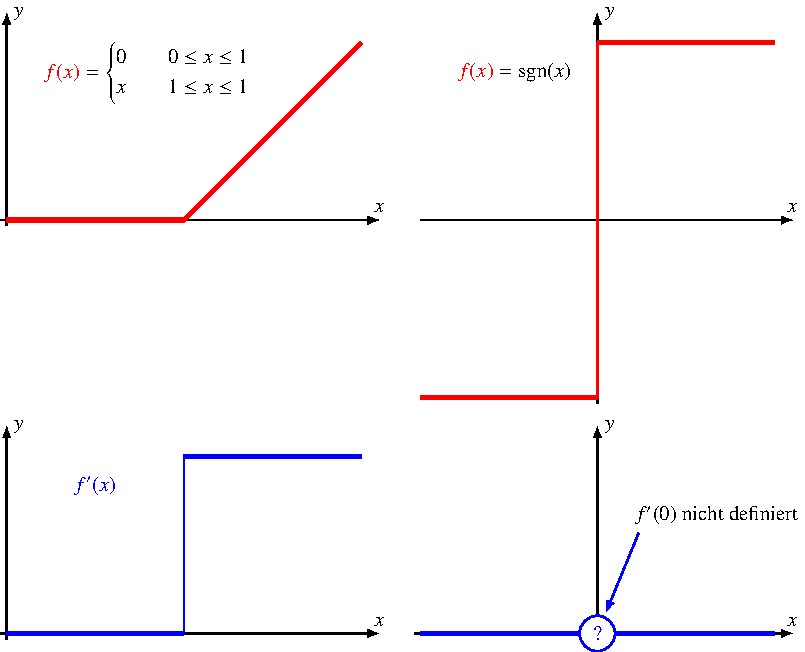
\includegraphics{chapters/010-skalarprodukt/images/schwach.pdf}
\caption{Schwache Ableitung einer nicht differenzierbaren Funktion.
Links die schwache Ableitung der Funktion von
Beispiel~\ref{buch:skalarprodukt:sobolevraum:bsp:schwachexistiert}.
Für die Signum-Funktion von
Beispiel~\ref{buch:skalarprodukt:sobolevraum:bsp:schwachexistiertnicht}
existiert die schwache Ableitung nicht, sie lässt für den Punkt $0$
nicht definieren.
\label{buch:skalarprodukt:sobolevraum:fig:schwach}}
\end{figure}
%
Die in Abbildung~\ref{buch:skalarprodukt:sobolevraum:fig:schwach} links
dargestellte Funktion
\[
f\colon (0,1) \to \mathbb{R}
:
x \mapsto
\begin{cases}
x&\qquad\text{für $0<x<1$}\\
1&\qquad\text{für $1\le x<2$}
\end{cases}
\]
ist stetig und integrierbar, aber sie ist an der Stelle $x=1$ nicht
differenzierbar.
Wir suchen die schwache Ableitung $v$ von $f$.

In einer Umgebung eines Punktes $x>1$ können wir Testfunktionen $\varphi$
so wählen, dass ihr Träger vollständig im Inneren des Intervals $(1,2)$
enthalten ist.
Mit diesen Testfunktionen können wir so rechnen, wie wenn $f$ die konstante
Funktion $1$ ist.
Das bedeutet für das Skalarprodukt
\[
\langle f,\varphi'\rangle
=
\int_1^2 \varphi'(x)\,dx
=
[\varphi(x)]_0^1 = 0.
\]
Das Skalarprodukt mit jeder beliebigen Testfunktion ist $0$, wir
müssen also $v(x)=0$ wählen.

Für $x$ im Teilinterval $(0,1)$ können wir die Testfunktionen so wählen,
dass der Träger vollständig im Inneren  von $(0,1)$ enthalten ist und
somit $f$ als die beliebig oft stetig differenzierbare Funktion $x$
behandelt werden darf.
Für das Skalarprodukt folgt dann
\[
-\langle f,\varphi'\rangle
=
-\int_0^1 f(x)\,\varphi'(x)\,dx
=
-\int_0^1 x\varphi'(x)\,dx
=
-[x\varphi(x)]_0^1 +\int_0^1 \varphi(x)\,dx
=
\langle 1,\varphi(x)\rangle,
\]
in diesem Teil des Intervals muss die schwache Ableitung den Wert $1$ 
haben.

Wir haben somit gefunden, dass die schwache Ableitung von $f$ die
Funktion
\[
v(x) = \begin{cases}
1&\qquad\text{für $0\le x<1$}
\\
0&\qquad\text{für $1< x<2$}
\end{cases}
\]
ist.
Wir kontrollieren dies, indem wir das Skalarprodukt für beliebige 
Testfunktionen $\varphi$ nachrechnen:
\begin{align*}
\langle v,\varphi\rangle
&=
\int_0^2 v(x)\,\varphi(x)\,dx
=
\int_0^1 1\,\varphi(x)\,dx
+
\int_1^2 0\,\varphi(x)\,dx.
\intertext{Jedes dieser Integrale kann man partiell integrieren:}
&=
[x\varphi(x)]_0^1 - \int_0^1 x\varphi'(x)\,dx
+
[1\varphi(x)]_1^2 - \int_1^2 1\varphi'(x)\,dx
\\
&=
\varphi(1) + \varphi(2) - \varphi(1) - \int_0^2 f(x)\,\varphi'(x)\,dx.
\intertext{Da $2$ ein Randpunkt ist, ist $\varphi(2)=0$, so dass sich}
&=-\langle f,\varphi'\rangle.
\end{align*}
ergibt.
Die Funktion $v$ ist also die schwache Ableitung von $f$.
\end{beispiel}

Eine Funktion in $W^{1,2}(\Omega)$ hat eine schwache Ableitung,
wie das Beispiel gezeigt hat, muss die Ableitung keine stetige
Funktion sein.
Ausserdem ist jede andere Funktion, die sich von der schwachen
Ableitung auf einer Menge vom Mass 0 unterscheidet, genauso eine
schwache Ableitung.
Trotzdem kann eine Funktion mit einer schwachen Ableitung nicht
beliebig ``wild'' sein, wie das folgende Beispiel zeigt.

\begin{beispiel}
\label{buch:skalarprodukt:sobolevraum:bsp:schwachexistiertnicht}
Die Signum-Funktion
\[
f\colon (-1,1) = \operatorname{sgn}(x) =
\begin{cases}
         - 1&\qquad\text{für $-1<x<0$}\\
\phantom{-}0&\qquad\text{für $x=0$}\\
\phantom{-}1&\qquad\text{für $0<x<1$}
\end{cases}
\]
ist nicht stetig (Abbildung~\ref{buch:skalarprodukt:sobolevraum:fig:schwach}).
$f$ ist fast überall konstant, in beiden Teilintervallen $(-1,0)$ und
$(0,1)$ ist die einzige mögliche schwache Ableitung von $f$ die
Nullfunktion.
Trotzdem kann $0$ nicht die schwache Ableitung von $f$ sein.
Wir wählen eine Testfunktion $\varphi$, die im Punkt $x=0$ von
Null verschieden ist.
Wäre $v$ eine schwache Ableitung von $f$, dann müsste
\begin{align*}
\langle v,\varphi\rangle
&=
-\langle f,\varphi'\rangle
=
-\int_{-1}^1 f(x) \varphi'(x)\,dx
\\
&=
-\int_{-1}^0 (-1)\cdot \varphi'(x)\,dx
-\int_{0}^1 1\cdot \varphi'(x)\,dx
=
\int_{-1}^0 \varphi'(x)\,dx
-
\int_{0}^1 \varphi'(x)\,dx
\\
&=
[\varphi(x)]_{-1}^0
-
[\varphi(x)]_{0}^1
=
\varphi(0)-\varphi(-1)
-
\varphi(1)+\varphi(0)
\\
&=
2\varphi(0)
\ne 0.
\end{align*}
Andererseits ist die Nullfunktion der einzige Kandidat für die
schwache Ableitun, für die das Skalarprodukt $\langle v,\varphi\rangle=0$
ist.
Dieser Widerspruch zeigt, dass die Funktion $f$ kein schwache
Ableitung hat.
\end{beispiel}

Die schwache Ableitung ermöglicht also mit gewissen Funktionen zu arbeiten,
die keine Ableitung im traditionellen Sinne haben.
Dank der Definition mit Hilfe eines Skalarproduktes in einem 
Hilbert-Raum darf man sich die Funktionen als Grenzwerte von
Cauchy-Folgen vorstellen.

%
% Physikalische Rechtfertigung
%
\subsection{Physikalische Rechtfertigung der schwachen Ableitung}
Die schwache Ableitung ersetzt die mit Hilfe eines Differenzenquotienten
definierte Änderungsrate durch eine Änderungsrate, die durch Vergleich
mit einer in der Umgebung eines Punktes konzentrierten Testfunktion
ermittelt wird.
Auf den ersten Blick mag das als Konzession an die Präzision der Ideen
der Analysis erscheinen, die Newton erfunden hat, um die Physik auf eine
neue Grundlage zu stellen.
Dabei wird aber vergessen, dass der Differenialquotient eine physikalisch
nicht erreichbare Idealisierung darstellt.
Keine Messung kann in einem Punkt im geometrischen Sinn erfolgen.
Die Bestimmung einer Position eines Massepunktes zum Beispiel erfolgt
durch Beobachtung des Lichtes, das vom Massepunkt reflektiert wird.
Doch der Massepunkt ist kein Punkt im geometrischen Sinn, er ist ausgedehnt
über ein endliches Gebiet.
Auch ist die Messung nicht instantan, es wird Licht gemessen, welches
über ein Zeitintervall vom Massepunkt reflektiert wird.
Das Messresultat entsteht also notwendigerweise als Mittelwert der
Beobachtung einer sehr grossen Zahl von Photonen, die von verschiedenen
Stellen reflektiert wurden.
Ein solcher Mittelwert ist genau das, was ein Skalarprodukt
$\langle f,\varphi\rangle$ mit einer Testfunktion ermittelt.

Die Feldgleichungen der Elektrodynamik wurden von Maxwell ausgehend
von Faradays Ideen als partielle Differentialgleichungen formuliert.
Sie verknüpfen die Werte des elektrischen Feldes $\vec{E}$ und des
magnetischen Feldes $\vec{B}$ mit der Ladungsdichte $\varrho$
und der Stromdichte $\vec{\jmath}$, die die Felder erzeugen.
Doch sowohl die Ladungsdichte wie auch die Stromdichte sind Idealisierungen.
Ladungen und Ströme sind nicht stetig über den Raum verteilt, sondern 
in Elektronen oder Atomkernen konzentriert.
Die Ladungsdichte entsteht daraus durch Messung der Ladung in einem kleine
Raumgebiet und Mittelung, was man wieder als Skalarprodukt mit einer
Testfunktion beschreiben kann.

Das elektrische Feld wird gemessen, indem die Kraft auf eine Testladung
im Feld ermittelt wird.
Ausser den prinzipiellen Einschränkungen an die Genauigkeit der
Positionsmessung wissen wir auch aus der Quantenmechanik, dass so etwas
wie die exakte Position eines Teilchens nicht gibt, wir können nur eine
Wahrscheinlichkeitsverteilung dafür bekommen.
Die Kraft äussert sich in einer Geschwindigkeitsänderung, die aber erst
messbar wird, wenn man die Beschleunigung eine gewisse Zeit lang aufrecht
erhält.
Das Messresultat ist also wieder ein Mittelwert über viele Positionen
und Zeitpunkte, oder anders ausgedrückt ein Skalarprodukt mit einer
Testfunktion.

Weitere Beispiele kann man auch in der Fluiddynamik finden.
Die Navier-Stokes-Gleichungen beschreiben die Strömung eines Mediums
unter der Annahme, dass es durch die Dichte $\varrho$ und die
Geschwindigkeit exakt beschreiben lässt.
Das Medium setzt sich aber aus einzelnen Atomen zusammen, die Dichte
ist also bereits ein Mittelwertbildung.
Bei der Geschwindigkeit wird das Problem noch deutlicher.
Auch die Strömungsgeschwindigkeit eines Gases ist der Mittelwert der
Strömungsgeschwindigkeit der Teilchen. 
Die Geschwindigkeit einzelner Teilchen ist dabei meistens sehr viel
grösser, nämlich im Bereich der Schallgeschwindigkeit, und äussert sich
in der Temperatur des Gases, also der mittleren kinetischen Energie.
Es ist nicht sinnvoll, von der Temperatur eines einzelnen Atoms zu
sprechen.

Alle diese Beispiele zeigen, dass die Ableitung als Änderungsrate, die
mit einem Differenzenquotienten bestimmt werden kann, eine Idealisierung
ist.
Wir können dies sogar etwas formeller zeigen.
Sei $x(t)$ die Koordinate eines Massepunktes zur Zeit $t$.
Die Messung kann nicht instantan erfolgen, im besten Fall ist die
gemessene Position ein Integral der Form
\[
\hat{x}(t)
=
\int_{-\infty}^\infty x(\tau) \varphi(\tau - t)\,d\tau.
\]
Darin ist $\varphi$ eine Testfunktion mit Träger in der Nähe von $0$.
Schreiben wir $T_t\varphi(\tau) = \varphi(\tau -t)$, dann können wir
das Messresultat auch als Skalarprodukt
$\hat{x}(t)=\langle x,T_t\varphi\rangle$
schreiben.
Die Messung mit der gleichen Aparatur einen Moment $\Delta t$ später ergibt
\[
\hat{x}(t+\Delta t)
=
\int_{-\infty}^\infty x(\tau) \varphi(\tau-t-\Delta t)\,dt
=
\langle x, T_{t+\Delta t}\varphi\rangle.
\]
Die Geschwindigkeit als Differenzenquotient ist
\begin{equation}
\frac{
\hat{x}(t+\Delta t)-\hat{x}(t)
}{\Delta t}
=
\frac{
\langle f,T_{t+\Delta t}\varphi\rangle
-
\langle f,T_{t}\varphi\rangle
}{
\Delta t
}
=
\left\langle
f,\frac{T_{t+\Delta t}\varphi - \varphi}{\Delta t}
\right\rangle
\label{buch:skalarprodukt:sobolevlraum:eqn:geschwindigkeit}
\end{equation}
Die Funktion $(T_{t+\Delta t}\varphi-T_t\varphi)/\Delta t$ ist eine 
beliebig oft stetig differenzierbare Funktion, die im Grenzwert
$\Delta t\to 0$ gegen
\[
\frac{
\varphi(\tau - t - \Delta t)
-
\varphi(\tau - t)
}{
\Delta t
}
=
-
\frac{
\varphi(\tau - t + \delta) - \varphi(\tau - t)
}{
\delta
}
\to 
-
\varphi'(\tau - t)
\quad
\text{für $\delta = - \Delta \to 0$}
\]
konvergiert.
Der Differenzenquotient
\eqref{buch:skalarprodukt:sobolevlraum:eqn:geschwindigkeit}
konvergiert daher gegen
\[
\lim_{\Delta t\to 0}
\frac{
\hat{x}(t+\Delta t)-\hat{x}(t)
}{\Delta t}
=
\left\langle
x,
\lim_{\Delta t\to 0}
\frac{T_{t+\Delta t}\varphi-T_t\varphi}{\Delta t}
\right\rangle
=
\langle f,-\varphi'\rangle
=
-
\langle f, \varphi'\rangle.
\]
Dieses einfache Modell einer ``unscharfen'' Messung führt also automatisch
auf das Konzept der schwachen Ableitung.








%\uebungsabschnitt
%\aufgabetoplevel{chapters/010-potenzen/uebungsaufgaben}
%\begin{uebungsaufgaben}
%\uebungsaufgabe{101}
%\uebungsaufgabe{102}
%\uebungsaufgabe{103}
%\uebungsaufgabe{104}
%\end{uebungsaufgaben}
%\endgroup



% more chapters

%\begin{appendices}
%\end{appendices}
\vfill
\pagebreak

\ifodd\value{page}\else\null\clearpage\fi
\lhead{Literatur}
\rhead{}
\printbibliography[heading=subbibliography]
\label{buch:literatur}

\end{refsection}


